% Possible use http://www.latextemplates.com/template/the-legrand-orange-book as template? See https://www.overleaf.com/9174958nyjxxdxbchks#/33024595/

\documentclass[11pt,letterpaper,fleqn]{memoir} % Default font size and left-justified equations


\usepackage[top=3cm,bottom=3cm,left=3cm,right=3cm,headsep=10pt,letterpaper]{geometry} % Page margins

\usepackage{assumptionsofphysics}
\frenchspacing

% Latex symbol guide at http://mirrors.ibiblio.org/CTAN/info/symbols/comprehensive/symbols-letter.pdf

\usepackage{float} % Required to use H for a figure so that it can be in the mathSection (i.e. minipage?)
\usepackage{xcolor} % Required for specifying colors by name
\definecolor{sectionNumbers}{RGB}{44, 103, 0}



% Style for math section
\RequirePackage[framemethod=default]{mdframed} % Required for creating the theorem, definition, exercise and corollary boxes
\newmdenv[skipabove=7pt,
skipbelow=7pt,
rightline=false,
leftline=true,
topline=false,
bottomline=false,
linecolor=sectionNumbers,
backgroundcolor=black!2,
innerleftmargin=5pt,
innerrightmargin=5pt,
innertopmargin=5pt,
leftmargin=0cm,
rightmargin=0cm,
linewidth=4pt,
innerbottommargin=5pt]{mathSection}


%----------------------------------------------------------------------------------------
%	SECTION NUMBERING IN THE MARGIN
%----------------------------------------------------------------------------------------

\makeatletter
\renewcommand{\@seccntformat}[1]{\llap{\textcolor{sectionNumbers}{\csname the#1\endcsname}\hspace{1em}}}                    
\renewcommand{\section}{\@startsection{section}{1}{\z@}
	{-4ex \@plus -1ex \@minus -.4ex}
	{1ex \@plus.2ex }
	{\normalfont\large\sffamily\bfseries}}
\renewcommand{\subsection}{\@startsection {subsection}{2}{\z@}
	{-3ex \@plus -0.1ex \@minus -.4ex}
	{0.5ex \@plus.2ex }
	{\normalfont\sffamily\bfseries}}
\renewcommand{\subsubsection}{\@startsection {subsubsection}{3}{\z@}
	{-2ex \@plus -0.1ex \@minus -.2ex}
	{.2ex \@plus.2ex }
	{\normalfont\small\sffamily\bfseries}}                        
\renewcommand\paragraph{\@startsection{paragraph}{4}{\z@}
	{-2ex \@plus-.2ex \@minus .2ex}
	{.1ex}
	{\normalfont\small\sffamily\bfseries}} % Loads the book formatting
\usepackage{tikz,pgfplots}
\usepackage[]{hyperref}

\newif\ifdraft

%\drafttrue
\draftfalse
\makeatletter
\@addtoreset{chapter}{part}
\makeatother 

\newcommand{\bookversion}{2.0}
\newcommand{\bookdate}{October 1, 2023}

% Adding ability to include pdfs (used to import book cover)
\usepackage{pdfpages}

% Adding pdf index and links within the document
% Custom formatting to remove default red boxes
\usepackage{hyperref}
\hypersetup{
	colorlinks=true,
    urlcolor=blue,
    linkcolor=blue
}
\urlstyle{same}
% ---------------------------

\usetikzlibrary{positioning,calc,arrows,arrows.meta, shapes,decorations.markings}


\begin{document}
	
% Set theory (expected) \in, \subset, injective/surjective, cartesian product

% Closure of a set under an operation

% Need examples of topology and sigma algebra

% Note that sigma algebra are also closed under intersections

% TODO: language change. Possibilities are experimentally DEFINED cases. Experimentally distinguishable cases give Hausdorff.

\frontmatter
\thispagestyle{empty} % Suppress headers and footers on the title page
\includepdf{BookCover.pdf}
\newpage
\thispagestyle{empty}
~
\newpage

~
\thispagestyle{empty}

\vspace{20pt}

{\large \noindent Gabriele Carcassi, Christine A. Aidala }

\vspace{60pt}

{\Huge \noindent \textbf{Assumptions of physics}}

\vspace{30pt}

\ifdraft {\large \noindent Working DRAFT for Ver \bookversion  ~- \today}
\else {\large \noindent Ver \bookversion  ~- \bookdate}
\fi

\vfill

%\chapter*{Assumptions of physics}

\ifdraft 
\noindent \textbf{This book is a work in progress}. This draft is a development copy built on \today. It is provided as-is for the purpose of early review and feedback. You can get the latest draft from \url{https://assumptionsofphysics.org/book}. 
\else
\noindent This edition was finalized on \bookdate. Older and newer versions can be found at  \url{https://assumptionsofphysics.org/book}.
\fi

\newpage
~\vfill
\thispagestyle{empty}

% Copyright notice
\noindent Copyright \copyright\ 2018-23 Gabriele Carcassi, Christine A. Aidala

\vspace{12pt}

% Link to website
\noindent \textsc{assumptionsofphysics.org/book}

\vspace{12pt}

% License
\noindent Licensed under the Attribution-NonCommercial-ShareAlike 4.0 International (CC BY-NC-SA 4.0) (the ``License"). You may not use this file except in compliance with the License. You may obtain a copy of the License at https://creativecommons.org/licenses/by-nc-sa/4.0/. This work is distributed under the License ``as is'', without warranties or conditions of any kind, either express or implied.

\chapter{Preface}

This work is part of a larger project, Assumptions of Physics (\url{https://assumptionsofphysics.org}), that aims to identify a handful of physical principles from which the basic laws can be rigorously derived. The goal is to give physics (and science more in general) a renewed foundation that is mathematically precise, physically meaningful and philosophically consistent. Given the ambition and broad scope of the task, nothing would ever be written if one were to wait for the complete picture. Therefore this work contains only the parts of the project that are considered to be mature, and so it will be revised and expanded as progress is made. We give here a brief overview of the project, which can be useful to better understand the context of this work.

\subsection{Overall goals of Assumptions of Physics}

What do the basic laws of physics describe? Why is the state of a classical particle identified by position and momentum (i.e.~a point on a symplectic manifold) while the state of a quantum system is identified by a wave function (i.e.~a vector in a Hilbert space)? What assumptions are unique to each theory? What are, instead, the basic requirements that all physical theories must satisfy? Could we have had different laws? A lack of clear answers to these questions is, we believe, the biggest obstacle in the foundations of physics and prevents the resolution of outstanding problems in the field. \textbf{Our approach is to find a minimal set of physical assumptions that are necessary and sufficient to derive the different theories within a unified framework.} If we are able to do so, then we are guaranteed that all that the laws of physics say is encoded in those assumptions and we are able to answer those questions.

We found this approach to be very fruitful. It provides new insights into physics as a whole, the role of mathematics in physical theories and a gives a more solid conceptual foundation to both. It becomes clear why some mathematical structures are pervasive in science and what exactly they are meant to represent, while others will never play a role. The downside is that we have to touch many subjects in math (logic, topological spaces, measure theory, group theory, vector spaces, differential geometry, symplectic geometry, statistics, probability theory, ...), physics (Hamiltonian mechanics, Lagrangian mechanics, thermodynamics, quantum mechanics, electromagnetism, ...) and science in general (computer science theory, information theory, system theory, ...). In other words, \textbf{the only way to properly achieve the goal is to rebuild everything from the ground up:} formal rigor, physical significance and conceptual integrity are not something that can be added at the end, but they must be present from the beginning.

The main takeaway for us is that the foundations of science are one: no real progress can be made on the foundations of one subject without making progress on the foundations of others. \textbf{What is needed is a general theory of experimental science: a theory that studies physical theories.} This provides a standard framework that defines basic concepts and requirements (e.g.~experimental verifiability, granularity of descriptions, processes and states) that serve as a common basis for all theories. Each theory, then, is recovered by studying how these common objects become specialized under different assumptions. This book aims to build over time, piece by piece, this framework.

While the topic is necessarily inter-disciplinary, \textbf{this is still first and foremost a scientific book}. The material should be accessible to the mathematician and philosopher, but understand that it needs to resonate first and foremost with the experimental physicist and the engineer. The mathematical definitions and derivations are there to make the science precise, but they are not the main focus. In fact, the book is designed so that the mathematical definitions and proofs, highlighted with a green side bar, can be skipped altogether without loss of the big picture and the important details. Along the same line, the foundational discussions are there to articulate more precisely what it means to do science, so they will not indulge in other questions which may be of interest to the philosopher but not to the scientist.

\subsection{A living work}

For the project to be successful, we need to depart from some of the norms of academic research and academic publishing. For example, one typically develops his research program as a series of articles published in a peer reviewed journal that caters to a specific community. These articles are then typically collected as is or merged into a book. This does not work for this project. As journals are specialized into sometimes very narrow fields, this would create a set of disjoint articles that cater to different audiences, with no guarantee that they can fit into a unified vision. For us, the overall picture, if and how the different perspectives combine, is the most important feature. \textbf{In this sense, the book comes first and the articles are derivative works.} We need to pool expertise and ideas from a wide range of disciplines and make sure that the result makes sense from all angles.

As the goal is broad, the framework needs to evolve as new issues are solved and old ones are better understood. If one part changes, we have to make sure that everything is updated to keep conceptual consistency. \textbf{This book, therefore, is an ongoing project.} It will continue to grow organically, adding and revising chapters. As is standard practice in open source/free software communities, we need to ``release early, release often'' to gather feedback. Each new version supersedes all prior ones and will be superseded by future ones. There is therefore no ``definitive version'' in the near future as we don't expect to ``solve all of physics'' in the near future. However, the framework will tend to converge as different parts become more settled.

The upshot is that one only needs to read the latest version of this work to be current. That is, one does not need to read a scattered set of papers, which require previous knowledge of a field, and follow how the ideas have changed. Just get the latest copy of the book, and if you do find areas you can help us expand or improve, let us know!

\section{Project overview}

Here we present a summary of the whole project and the status of each part as the layout will map to the structure of this work. We divide the work based on the two main techniques we use. The first, \textbf{reverse physics}, aims to identify the fundamental ideas and assumptions by reverse engineering them from the current physical theories. The second, \textbf{physical mathematics}, aims to construct a rigorous mathematical framework from the ground up, based on the ideas and assumptions found by reverse physics.


\subsection{Reverse physics}

Reverse physics looks at the main physical theories, like classical mechanics, thermodynamics and quantum mechanics, to identify concepts that can be used to fully explain the common and different aspects of those theories. The idea is to find physically meaningful assumptions that can be shown to be equivalent to the physical laws.

The standard of rigor in this part is necessarily more relaxed as we do not have a guarantee that sufficiently mature mathematical tools exist to carry out the argument in a precise fashion. For example, we have found that the idea of a unit system is linked in a fundamental way to the notion of state spaces, yet we lack a fully developed mathematical framework to model units and their dependency. The goal is to test the ideas conceptually, find those that are broad enough and necessary enough to then justify investing further time in a more rigorous approach.

The following are examples of the type of assumptions we have found to be good starting points to rederive the different theories.

\begin{description}
	\item[Determinism and reversibility:] ``The system undergoes deterministic and reversible evolution." Mathematically, the physical properties of the system determine which category, in the mathematical sense, is used to describe the state space, and deterministic and reversible evolution will be an isomorphism in the category (i.e.~a bijective map that preserves the physical properties of the system). Therefore the law of evolution is not just a bijective map, but is also a linear transformation, a differentiable map or an isometry depending on the context.
	
	\item[Infinitesimal reducibility:] ``Specifying the state of the whole system is equivalent to specifying the state of all its infinitesimal parts." For example, we can study the motion of a ball, but we can also mark a spot in red and study the motion of the mark. Knowing the evolution of the whole ball means knowing the evolution of any arbitrary spot and vice-versa. Mathematically, the state of the whole will be a distribution over the state space of the parts. It will need to be a distribution whose value is invariant under coordinate transformations. The state space of the infinitesimal parts, then, comes equipped with an invariant two-form upon which we can define such a distribution. The state space is therefore a symplectic manifold, that is,
	the states of the infinitesimal parts are described by pairs of conjugate variables, which recovers phase space. If the previous assumption holds, deterministic and reversible evolution is a symplectomorphism, that is,  deterministic and reversible evolution follows classical Hamiltonian mechanics. Proper handling of the time variable will give us a relativistic version of the framework without extra assumptions.
	
	\item[Irreducibility:] ``Specifying the state of the whole system tells us nothing about its infinitesimal parts." For example, we can study the state of an electron by scattering photons off of it. But whenever a photon interacts with the electron, it interacts with the whole electron. There is no way to mark a part of an electron and study it independently from the rest. Mathematically, the state of the electron will be a distribution that evolves deterministically where the motion of each infinitesimal part cannot be further described.
	
	\item[Kinematic equivalence:] ``Specifying the motion of the system is equivalent to specifying its state and evolution." This means that we will have to be able to re-express a distribution over kinematic variables (i.e.~position and velocity) into a distribution over state variables (i.e.~position and momentum) and vice-versa. Mathematically, the symplectic two-form will induce a symmetric tensor over the tangent space for position. This will give us a metric and will also allow us to reformulate the laws of motion according to Lagrangian mechanics. Because the transformation is linear, we are able to constrain the Hamiltonian to the one for massive particles under scalar and vector potential forces.
\end{description}


\subsection{Physical mathematics}

The first step in physical mathematics is the development of a general mathematical theory of experimental science, or simply a general theory, that lays down the basic axioms and definitions that are required for any physical theory. \textbf{We need a ``theory of scientific theories'' that allows us to define and study the set of all well-formed scientific theories.} The core tenet is the principle of scientific objectivity: ``Science is universal, non-contradictory and evidence based.'' This serves to define the subject and the basic formal requirements of a scientific theory. We divide the general theory into three main parts.

\begin{description}
	\item[Experimental verifiability.] This part defines a scientific theory as a set of statements. It provides the basic axioms which simply characterize the rules of logic as applied to experimentally verifiable statements. Mathematically, these requirements are captured by topologies and $\sigma$-algebras over the space of the possible cases that can be identified experimentally. This part is very well developed both conceptually and mathematically, and it is the only part currently included in this book. 
	
	\item[Informational granularity.] This part adds the ability to compare the level of description of different statements. Mathematically, this imposes a preorder on the algebra of statements which is intended to provide a common foundation to geometry, measure theory, probability theory and information theory. All those structures, in fact, provide ways to compare the size of sets of possible cases and the description provided in terms of those sets. This part is fairly developed conceptually but not yet well developed mathematically.
	
	\item[States and processes.] This part defines the basic physical notions of processes, systems and states. It serves to bring to light a series of hidden assumptions that are needed, both physically and mathematically, to be able to talk about independent systems. These will lead to notions of entropy, state spaces and the geometrical structures that accompany them. This part is still being developed conceptually, though the progress is encouraging.
\end{description}


\section*{Current plan and status}

In this version we have added a reverse physics part with a chapter on classical mechanics. We plan to follow that with a chapter on thermodynamics and statistical mechanics. For physical mathematics, the work is slowed down by the fact that general mathematical tools for the informational granularity appear to be missing. In particular, if we want state counting in quantum mechanics to be consistent with statistical mechanics and information theory, a more general notion of measure is needed.

\section*{Changelog}

\begin{description}
	\item 2023/10/01: Ver 2.0 - Divided the work into two main parts: Reverse Physics and Physical mathematics. Added chapter on reversing classical mechanics. Minor updates on the logic section.
	\item 2021/03/08: Ver 1.0 - Updated the first three chapters with minor changes: renamed tautology to certainty and contradiction to impossibility as they characterize better their role in the framework; made more formal justifications for the basic axioms and some of the basic definitions; causal relationships are now proved to be continuous instead of assumed to be continuous. Added Part II to include the results that are not yet fully formalized, to give a sense of the future scope of the work.
	\item 2019/07/07: Ver 0.3 - Reviewed first two chapters to clarify the idea of possible assignments and how contexts for function spaces are constructed.
	\item 2019/02/22: Ver 0.2 - Consolidated third chapter on properties, quantities and ordering.
	\item 2018/06/22: Ver 0.1 - Consolidated first two chapters that lay the foundation for the general theory.
\end{description}


\cleardoublepage % Forces the first chapter to start on an odd page so it's on the right

\tableofcontents* % Print the table of contents itself

\cleardoublepage % Forces the first chapter to start on an odd page so it's on the right

%\pagestyle{fancy} % Print headers again

\mainmatter

\part{Reverse Physics}
\begingroup
\pagestyle{plain}

\include{reverse-physics-intro}

\newpage
\endgroup


\newcommand{\eqtext}[2][4.5in]{\parbox{#1}{#2}}

\chapter{Classical mechanics}

The standard view in physics is that classical mechanics is perfectly understood. It has three different but equivalent formulations, the oldest of which, Newtonian mechanics, is based on three laws. Classical mechanics is the theory of point particles that follow those laws. Unfortunately, this view is incorrect.

We will see that the three formulations are not equivalent, in the sense that there are physical systems that are Newtonian but not Hamiltonian and vice-versa. There are also a number of questions that have been left unanswered, such as the precise nature of the Hamiltonian or the Lagrangian, and what exactly the principle of stationary action represents physically. While shedding light on these issues, we will also find that classical mechanics already contains elements that are typically associated with other theories, such as quantum mechanics/field theories (uncertainty principle, anti-particles), thermodynamics/statistical mechanics (thermodynamic and information entropy conservation) or special relativity (energy as the time component of a four-vector). In other words, the common understanding of classical mechanics is quite shallow, and its foundations are, in fact, not separate from the ones of classical statistical mechanics or special relativity.

What reverse physics shows is that the central assumption underneath classical mechanics is that of \textbf{infinitesimal reducibility (IR)}: a classical system can be thought of as made of parts, which in turn are made of parts and so on; studying the whole system is equivalent to studying all its infinitesimal parts. This assumption, together with the assumption of \textbf{independence of degrees of freedom (IND)}, is what gives us the structure of classical phase space with conjugate variables. The additional assumption of \textbf{determinism and reversibility (DR)}, the fact that the description of the system at one time is enough to predict its future or reconstruct its past, leads us to Hamiltonian mechanics. On the other hand, assuming \textbf{kinematic equivalence (KE)}, the idea that trajectories in space are enough to reconstruct the state of the system and vice-versa, leads to Newtonian mechanics. The combination of all above assumptions, instead, leads to Lagrangian mechanics and, in particular, to massive particles under (scalar and vector) potential forces.

As a guide to the chapter, here is the list of main points in the order in which they will be presented, one for each section.
\begin{enumerate}
	\item Review of classical formulations
	\item Lagrangian mechanics is Hamiltonian mechanics and KE
	\item Kinematics, in general, is not enough to reconstruct dynamics
	\item Hamiltonian mechanics (one DOF) is equivalent to DR
	\item Hamiltonian mechanics (multiple DOFs) is equivalent to DR plus IND
	\item Differential calculus and its generalization, differential topology, study infinitesimally additive quantities that depend on geometric shapes (i.e. lines, surfaces, volumes)
	\item The principle of least action is a consequence of DR, IND and KE
	\item Massive particles under potential forces are a consequence of DR, IND and KE
	\item Special relativity is a consequence of DR, IND and KE
	\item Phase space is the only structure that makes distributions, state counting and entropy frame invariant
	\item Newtonian mechanics is a consequence of KE
	\item Three dimensional spaces are the only spaces for which distributions over directions are frame invariant
	\item Classical particle states as points in phase space are equivalent to IR
\end{enumerate}

\section{Formulations of classical mechanics}

In this section we will briefly review the three main formulations of classical mechanics. Our task is not to present them in detail, but rather to provide a brief summary of the equations so that we can proceed with the comparison. In particular, given that different conventions are used across formulations, within the same formulation and among different contexts (e.g. relativity, symplectic geometry), we will want to make the notation homogeneous to allow easier comparisons.

\subsection{Newtonian mechanics}

For all formulations, the system is modeled as a collection of point particles, though we will mostly focus on the single particle case. For a Newtonian system, the state of the system at a particular time $t$ is described by the position $x^i$ and velocity $v^i$ of all its constituents. Each particle has its mass $m$, not necessarily constant in time, and, for each particle, we define kinetic momentum as $\Pi^i = m v^i$.\footnote{We will use the letter $t$ for the time variable, $x$ for position and $v$ for velocity, which is a very common notation in Newtonian mechanics. However, we will keep using the same letters in Lagrangian mechanics as well, instead of $q$ and $\dot{q}$, for consistency. Given that the distinction between kinetic and conjugate momentum is an important one, we will denote $\Pi$ the former and $p$ the latter. The Roman letters $i,j,k,...$ will be used to span the spatial components (e.g. $i \in \{1,2,3\}$ for a particle in 3 dimensional space and $i \in \{1,2,\dots, 3n\}$ for n particles), while we will use the Greek letters $\alpha, \beta, \gamma, ...$ to span space-time components (e.g. $\alpha \in \{0,1,2,3\}$ where the $0$ value of the index is used for time). Unlike some texts, $x^i$ do not represent Cartesian coordinates, and therefore they should be understood already as generalized coordinates.}

The evolution of our system is given by Newton's second law:\footnote{For derivatives, we will use the shorthand $d_t$ for $\frac{d}{dt}$ and $\partial_{x^i}$ for $\frac{\partial}{\partial x^i}$. For functions that depend on multiple arguments we use a free index to note that it depends on all elements; each argument will have a different index to highlight that there is no relationship between arguments. }
\begin{equation}\label{rp-cm-NewtonsSecondLaw}
	F^i(x^j, v^k, t) = d_t \Pi^i.
\end{equation}
Mathematically, if the forces $F^i$ are locally Lipschitz\footnote{Lipschitz continuity means that the slope of the function is bounded. For example, $\sqrt{x}$ in the neighborhood of $0$ is not Lipschitz continuous as it has a vertical asymptote at that point. One can construct examples (e.g. Norton's dome) where the forces are not locally Lipschitz continuous, and therefore the initial position and velocity do not yield a unique solution (i.e. in Norton's dome, the body can stay on the top of the dome indefinitely, or it can fall down after an arbitrary amount of time). In this case, something else, outside the system, will necessarily determine what is the motion of the system, and therefore it is not true that the force and the state of the system fully determine the dynamics of the system.} continuous, then the solution $x^i(t)$ is unique. That is, given position and velocity at a given time, we can predict the position and velocity at future times. We will assume a Newtonian system has this property.

An important aspect of Newtonian mechanics is that the equations are not invariant under coordinate transformation. To distinguish between apparent forces (i.e. those dependent on the choice of frame) and the real ones, we assume the existence of inertial frames. In an inertial frame there are no apparent forces, and therefore a free system (i.e. no forces) with constant mass proceeds in a linear uniform motion, or stays still.\footnote{Recall that linear motion simply means that it describes a line in space, while uniform motion means that the speed is constant. Therefore we can have linear non-uniform motion (e.g. an object accelerated along the same direction) or a non-linear uniform motion (e.g. an object going around in a circle at constant speed).}

\subsection{Lagrangian mechanics}

The state for a Lagrangian system is also given by position $x^i$ and velocity $v^i$. The dynamics is specified by a single function $L(x^i, v^j, t)$ called the Lagrangian. For each spatial trajectory $x^i(t)$ we define the action as $\mathcal{A}[x^i(t)] = \int_{t_0}^{t_1} L(x^i(t), d_t x^i(t), t) dt$. The trajectory taken by the system is the one that makes the action stationary:
\begin{equation}
\delta \mathcal{A}[x^i(t)] = \delta \int_{t_0}^{t_1} L\left(x^i(t), d_t x^i(t), t\right) dt=0
\end{equation}
The evolution can equivalently be specified by the Euler-Lagrange equations:
\begin{equation}\label{rp-cm-EulerLagrange}
	\partial_{x^i}L=d_t \partial_{v^i} L.
\end{equation}

%TODO: we should improve how the invertibility/Jacobian \neq 0 is handles. Technically, if we only require invertibility, the Jacobian is either positiove or negative semi-definite (it can be zero). However, if the relationship is differentiable, the zero case is excluded.

Note that not all Lagrangians lead to a unique solution. For example, $L=0$ will give the same action for all trajectories and therefore, strictly speaking, all trajectories are possible. The stationary action leads to a unique solution if and only if the Lagrangian is hyperregular, which means the Hessian matrix $\partial_{v^i}\partial_{v^j} L$ is invertible. Like in the Newtonian case, we will assume Lagrangian systems satisfy this property.

Unlike Newton's second law, both the Lagrangian and the Euler-Lagrange equations are invariant under coordinate transformations. This means that Lagrangian mechanics is particularly suited to study the symmetries of the system.

\subsection{Hamiltonian mechanics}

In Hamiltonian mechanics, the state of the system is given by position $q^i$ and conjugate momentum $p_i$. The dynamics is specified by a single function $H(q^i, p_j, t)$ called the Hamiltonian.\footnote{We use a different symbol for position in Hamiltonian mechanics because, while it is true that $q^i = x^i$, it is also true that $\partial_{q^i} \neq \partial_{x^i}$: the first derivative is taken at constant conjugate momentum while the second is taken at constant velocity. This creates absolute confusion when mixing and comparing Lagrangian and Hamiltonian concepts, which our notation avoids completely.} The evolution is given by Hamilton's equations:
\begin{equation}\label{rp-cm-HamiltonEq}
	\begin{aligned}
		d_t q^i = \partial_{p_i} H \\
		d_t p_i = - \partial_{q^i} H \\
	\end{aligned}
\end{equation}
We will again want these equations to yield a unique solution, which means the Hamiltonian must be at least differentiable, and the derivatives must at least be Lipschitz continuous.

Hamilton's equations are invariant as well. The Hamiltonian itself is a scalar function which is often considered (mistakenly as we'll see later) invariant. This formulation is the most suitable for statistical mechanics as volumes of phase space correctly count the number of possible configurations.

\section{Inequivalence of formulations}\label{rp-cm-inequivalenceOfFormulations}

It is often stated in physics books that all three formulations of classical mechanics are equivalent. We will look at this claim in detail, and conclude that this is not the case: there are systems that can be described by one formulation and not another. More precisely, the set of Lagrangian systems is exactly the intersection of Newtonian and Hamiltonian systems.

\subsection{Testing equivalence}

We will consider two formalisms equivalent if they can be applied to exactly the same systems. That is, Newtonian and Lagrangian mechanics are equivalent if any system that can be described using Newtonian mechanics can also be described by Lagrangian mechanics and vice-versa. In general, in physics great emphasis is put on systems that can indeed be studied by all three, leaving the impression that this is always doable.\footnote{If one asks the average physicist whether Newtonian and Hamiltonian mechanics are equivalent, the answer most of the time will be  enthusiastically positive. If one then asks for the Hamiltonian for a damped harmonic oscillator, the typical reaction is annoyance due to the nonsensical question (damped harmonic oscillators do not conserve energy), followed by a realization and partial retraction of the previous claim. The moral of the story is to never take these claims at face value.} However, just with a cursory glance, we realize that this can't possibly be the case.

The dynamics of a Newtonian system, in fact, is specified by three independently chosen functions of position and velocity, the forces applied to each degree of freedom (DOF). On the other hand, the dynamics of Lagrangian and Hamiltonian systems is specified by a single function of position and velocity/momentum, the Lagrangian/Hamiltonian. Intuitively, there are more choices in the dynamics for Newtonian systems than for Lagrangian and Hamiltonian.

Now, the reality is a bit trickier because the mathematical expression of the forces is not enough to fully characterize the physical system. We need to know in which frame we are, what coordinates are being used and the mass of the system, which is potentially a function of time. On the Lagrangian side, note that the Euler-Lagrange equations are homogeneous in $L$. This means that multiplying $L$ by a constant leads to the same solutions, meaning that the same system can be described by more than one Lagrangian. The converse is also true: if one system is half as massive and is subjected to a force half as intense, the resulting Lagrangian is also simply rescaled by a constant factor. Therefore the map between Lagrangians and Lagrangian systems is not one-to-one: it is many-to-many. This is why we should never look simply at mathematical structures if we want to fully understand the physics they describe.

Regardless, our task is at the moment much simpler: we only need to show that there are Newtonian systems not expressible by Lagrangian or Hamiltonian mechanics. We can therefore limit ourselves to systems with a specific constant mass $m$ in an inertial frame and write $a^i=F^i(x^j, v^k, t)/m$. Given that the force is arbitrary, the acceleration can be an arbitrary function of position, velocity and time. Similarly, we can write the acceleration of a Lagrangian system as $a^i=F^i[L]/m$. That is, the acceleration is going to be some functional of the Lagrangian. Given the Euler-Lagrange equations \ref{rp-cm-EulerLagrange}, the map between the Lagrangian and the acceleration must be continuous in both directions: for a small variation of the Lagrangian we must have a small variation of the equations of motion and therefore of the acceleration, and for a small variation of the equations of motion we must have a small variation of the Lagrangian. But a continuous surjective map from the space of a single function (i.e. the Lagrangian) to the space of multiple functions (i.e. those that specify the acceleration in terms of position and velocity) does not exist,\footnote{Mathematically, the space of continuous functions $C(\mathbb{R}, \mathbb{R})$ and $C(\mathbb{R}^n, \mathbb{R})$ are not homeomorphic. Intuitively, the underlying reason is the same as to why a map from a volume to a line can't be continuous: in a volume you have infinitely many directions you can move away from a point, while on a line you only have two.} and therefore there must be at least one Newtonian system with constant mass expressed in an inertial frame that is not describable using Lagrangian mechanics. The same argument applies for Hamiltonian mechanics, since the dynamics in this case is also described by a single function in the same number of arguments. We therefore reach the following conclusion:
\begin{insight}
	Not all Newtonian systems are Lagrangian and/or Hamiltonian.
\end{insight}

\subsection{Newtonian vs Lagrangian/Hamiltonian}

We now want to understand whether all Lagrangian systems are Newtonian. Given what we discussed, we cannot expect to reconstruct the mass and force uniquely from the expression of the Lagrangian. We consider the mass and the frame fixed by the problem, together with the Lagrangian, and therefore we must only see whether we can indeed find a unique expression for the acceleration. From the Euler-Lagrange equations \ref{rp-cm-EulerLagrange} we can write
\begin{equation}
	\begin{aligned}
	\partial_{x^i}L&=d_t \partial_{v^i} L=\partial_{x^j} \partial_{v^i} L \, d_t x^j + \partial_{v^k} \partial_{v^i} L \, d_t v^k + \partial_{t} \partial_{v^i} L \, d_t t \\
	&= \partial_{x^j} \partial_{v^i} L \, v^j + \partial_{v^k} \partial_{v^i} L \, a^k + \partial_{t} \partial_{v^i} L \\
	\partial_{v^k} &\partial_{v^i} L \, a^k = \partial_{x^i}L - \partial_{x^j} \partial_{v^i} L \, v^j - \partial_{t} \partial_{v^i} L.
	\end{aligned}
\end{equation}
To be able to write the acceleration explicitly, we must be able to invert the Hessian matrix $\partial_{v^k} \partial_{v^i} L$. As we noted before, this is exactly the condition for which the principle of stationary action leads to a unique solution, and we can better understand why. If it is not invertible at a point, the determinant is zero and therefore one eigenvalue is zero. The corresponding eigenvector corresponds to a direction for which the equation tells us nothing, and therefore a variation of the acceleration in that direction will not change the action. This is why the invertibility of the Hessian is required in order to obtain unique solutions.

What we find, then, is that for any Lagrangian system, which we assume to have a unique solution, we can explicitly write the acceleration as a function of position, velocity and time. Therefore
\begin{insight}
	All Lagrangian systems are Newtonian.
\end{insight}

Now we turn our attention to Hamiltonian mechanics and, similarly, we ask whether we can express the acceleration as a function of the state. We have
\begin{equation}
	\begin{aligned}
		a^i &= d_t v^i = d_t d_t q^i = d_t \partial_{p_i} H = \partial_{q^j} \partial_{p_i} H d_t q^j + \partial_{p_k} \partial_{p_i} H d_t p_k + \partial_{t} \partial_{p_i} H d_t t\\
		&= \partial_{q^j} \partial_{p_i} H \partial_{p_j} H - \partial_{p_k} \partial_{p_i} H \partial_{q^k} H + \partial_{t} \partial_{p_i} H.
	\end{aligned}
\end{equation}
This tells us that we can always write an explicit function for the acceleration. However, this is not enough. States in Newtonian mechanics are in terms of position and velocity, not position and momentum. For a Hamiltonian system to be equivalent to a Newtonian system we need to be able to write the momentum as a function of position and velocity and vice versa. Note that Hamilton's equations already give a way to express the velocity in terms of position and momentum. We just need that expression to be invertible, which means the Jacobian must be invertible. We must have:
\begin{equation}
	\left|\partial_{p_i} v^j\right| = \left|\partial_{p_i}\partial_{p_j} H\right| \neq 0 .
\end{equation}
To be able to express momentum as a function of position and velocity, then, we need the Hessian of the Hamiltonian to be invertible (i.e. to have non-zero determinant).

Note that we had no such requirement for the Hamiltonian itself. For example, $H=0$ leads to equations $d_t q^i = 0$ and $d_t p_i = 0$, which have unique solutions: both position $q^i(t) = k_{q^i}$ and momentum $p_i(t) = k_{p_i}$ are constants of motion. The Hessian, being the zero matrix, is not invertible, and in fact we cannot write momentum as a function of position and velocity: velocity $d_t q^i$ is always zero in all cases while conjugate momentum can be any value $k_{p_i}$. Though this case may not be physically interesting, it is a perfectly valid Hamiltonian system and shows that we should always check the trivial mathematical case. However, let us go through a more physically meaningful case.

\begin{figure}
	\centering
	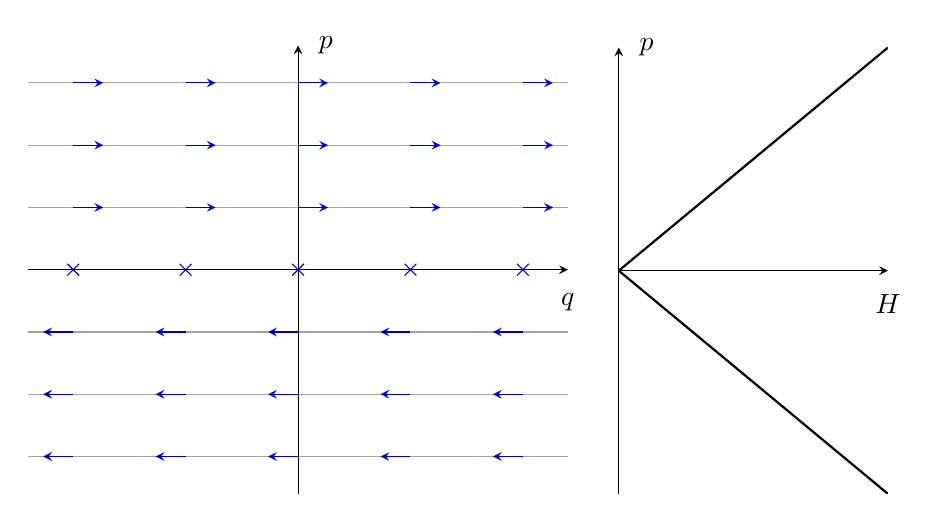
\begin{tikzpicture}
		\pgfplotsset{ticks=none}
		\begin{axis}[axis lines=middle,
			xlabel=$q$,
			xlabel style={below=5pt, fill=white},
			ylabel=$p$,
			ylabel style={above=2pt, right=4pt},
			domain=-1.5:1.5,
			ymin=-1.8, ymax=1.8,]
			\foreach \yvalue in {-1.5,-1,-0.5, 0.5, 1, 1.5} {
				\addplot[blue,-stealth,samples=5,
				quiver={
					u={y/abs(y)},
					v={0},
					scale arrows=0.2},
				] {\yvalue};
				\addplot[black,samples=2,opacity=0.2,domain=-1.8:1.8]{\yvalue};
				\addplot[black,samples=2,opacity=0.2,domain=-1.8:1.8]{\yvalue};}
			\addplot[scatter, only marks, mark size=3pt, samples=5, mark=x, color=green]{0};
		\end{axis}
		
		\pgfplotsset{ticks=none}
		\begin{axis}[
			xshift=7.5cm,
			width=5cm,
			height=7.25cm,				
			axis lines=middle,
			xlabel=$H$,
			xlabel style={below=5pt, fill=white},
			ylabel=$p$,
			ylabel style={above=2pt, right=4pt},
			domain=0:1,
			xmin=0, xmax=1,
			ymin=-1, ymax=1,]
			\addplot[black,thick,samples=2,domain=0:1]{x};
			\addplot[black,thick,samples=2,domain=0:1]{-x};
		\end{axis}
	\end{tikzpicture}
	\caption {On the left, the phase-space diagram for a photon treated as a point particle. The Hamiltonian $H=c|p|$, on the right, is proportional to the modulus of $p$. Since $H$ is not differentiable when $p=0$, those states are excluded, consistent with the physics. The displacement field has only a $q$ component, which is $+c$ above the horizontal axis and $-c$ below the horizontal axis. } \label{fig_rp_cm_photon}
\end{figure}

\textbf{Photon as a particle}. If we want to treat the photon as a classical particle, we can write the Hamiltonian by expressing the energy as a function of momentum
\begin{equation}
	H=\hbar | \omega| = c \hbar |k_i| = c |p_i|.
\end{equation}
If we apply Hamilton's equations, we have
\begin{equation}
	\begin{aligned}
		d_t q^i &= c \frac{p_i}{|p_i|} \\
		d_t p_i &= 0.
	\end{aligned}
\end{equation}
That is, the norm of the velocity is always $c$, the momentum decides its direction, and the momentum itself does not change in time, as shown in fig. \ref{fig_rp_cm_photon}. This is indeed the motion of a free photon. One can confirm, through tedious calculation, that the determinant of the Hessian is indeed zero, yet it is easier and more physically instructive to see that we cannot reconstruct the momentum from the velocity. Relativistically, all photons travel along the geodesics at the same speed, therefore two photons that differ only by the magnitude of the momentum will travel the same path.

Hamiltonian systems that are also Newtonian, then, need to satisfy this extra condition, so let us give it a name.
\renewcommand{\theassump}{KE}
\begin{assump}[Kinematic Equivalence]\label{assum_kineq}
	The kinematics of the system is sufficient to reconstruct its dynamics and vice-versa. That is, specifying the motion of the system is equivalent to specifying its state and evolution.
\end{assump}
\renewcommand{\theassump}{\Roman{assump}}
By kinematics we mean the motion in space and time and by dynamics we mean the state and its time evolution in phase space. We will need to analyze the difference between the two more in detail, but we should first finish our comparison between the different formulations.

Summing up, we find that
\begin{insight}
	Not all Hamiltonian systems are Newtonian: only those for which  \ref{assum_kineq} is valid.
\end{insight}

\subsection{Lagrangian vs Hamiltonian}

We now need to compare Lagrangian and Hamiltonian systems. The task is a lot easier because we already have a precise way to connect the two. If we are given a Lagrangian $L$, we define the conjugate momentum $p_i = \partial_{v^i} L$ and the Hamiltonian $H = p_i v^i - L$. If we are given a Hamiltonian $H$, we can define a Lagrangian $L = p_i v^i - H$ and a velocity $v^i = d_t q^i = \partial_{p_i} H$. However, this is a bit misleading: the above relationships connect the values of the functions for each state $s$. That is, $L(s) = p_i(s) v^i(s) - H(s)$. Both the Lagrangian and the Hamiltonian are functions of specific variables, so we have to make sure we can express them in the appropriate variables.

Going from a Hamiltonian to a Lagrangian, it again means that we can write momentum as a function of position and velocity, and therefore assumption \ref{assum_kineq} must hold. This makes sense: if all Lagrangian systems are Newtonian, and \ref{assum_kineq} was required for a Hamiltonian system to be Newtonian, then it is also required for a Hamiltonian system to be Lagrangian. But the connection is stronger: \ref{assum_kineq} is the \emph{only} additional assumption we need to be able to write a Lagrangian given a Hamiltonian.

Going from a Lagrangian to a Hamiltonian, it means that we can write velocity as a function of position and momentum. Note that since we define conjugate momentum as the derivative of the Lagrangian, we can already express momentum as a function of position and velocity, which means we are simply asking that expression to be invertible. This is, again, assumption \ref{assum_kineq}, just in the opposite direction. We must have
\begin{equation}
	0 \neq \left| \partial_{v^i} p_j \right| = \left| \partial_{v^i} \partial_{v^j} L \right|.
\end{equation}
This means that assumption \ref{assum_kineq} is exactly the invertibility of the Hessian, the condition for unique solution of the Lagrangian. All Lagrangian systems that admit unique solutions, then, satisfy assumption \ref{assum_kineq}. In fact, we can see that the Hessian determinants are related
\begin{equation}
	\left| \partial_{v^i} \partial_{v^j} L \right| = \left| \partial_{v^i} p_j \right| = \left| \partial_{p_i} v^j \right|^{-1} = \left|\partial_{p_i}\partial_{p_j} H\right|^{-1}.
\end{equation}
This means that every Lagrangian admits a Hamiltonian, but not every Hamiltonian admits a Lagrangian. Only the Hamiltonian systems for which \ref{assum_kineq} is valid will also be Lagrangian systems, with a guaranteed unique solution given that \ref{assum_kineq} is exactly the assumption needed for that as well. Therefore we conclude that
\begin{insight}
	Lagrangian systems are exactly those Hamiltonian systems for which \ref{assum_kineq} is valid.
\end{insight}

\subsection{Relationship between formulations}

The relationship between the different formulations, then, can be summarized with the Venn diagram in fig. \ref{rp-cm-fig-vennDiagramEarly}.

\begin{figure}[h]
	\centering
	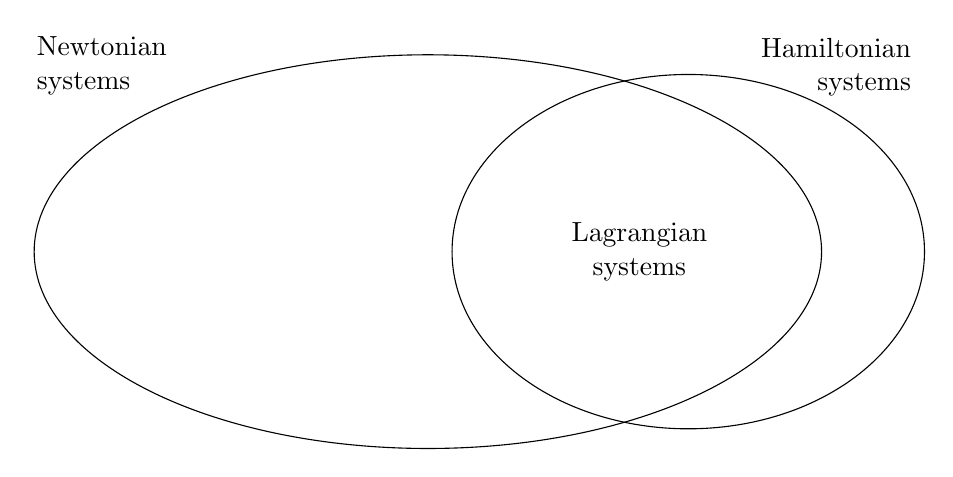
\begin{tikzpicture}
		\node[ellipse, minimum width=10cm, minimum height=5cm, draw, left] (ns){};
		\node [align=left, above] at ([xshift=-6mm,yshift=1mm]ns.north west) {Newtonian \\systems};
		
		\node[ellipse, minimum width=6cm, minimum height=4.5cm, draw] (hs) at ([xshift=-1.7cm]ns.east){};
		\node [align=right, above right] at ([xshift=8mm, yshift=-4mm]hs.north) {Hamiltonian\\ systems};
		\node [align=center, right] at ([xshift=14
		mm]hs.west) {Lagrangian \\systems};
	\end{tikzpicture}
	\caption {Not all Hamiltonian systems are Newtonian and not all Newtonian systems are Hamiltonian. All Lagrangian systems are both Newtonian and Hamiltonian.}\label{rp-cm-fig-vennDiagramEarly}
\end{figure}


We have found that \ref{assum_kineq} is a constitutive assumption of Lagrangian mechanics, and that it clearly marks which Hamiltonian systems are Newtonian/Lagrangian. By constitutive assumption we mean an assumption that must be taken, either explicitly or implicitly, for a theory to be valid. But what makes a system Hamiltonian and what makes a system Newtonian? Can we find a full set of constitutive assumptions for classical mechanics?

\section{Kinematics vs dynamics}

We have seen the importance of the connection between kinematics and dynamics. In this section we will explore this link more deeply and come to the following conclusion: the kinematics of a system is not enough to reconstruct its dynamics. 

\subsection{Particle under linear drag}

Let us first review exactly what the kinematics and dynamics are. Given a system, its kinematics is the description of its motion in space and time. Position, velocity, and acceleration are kinematic variables because they describe the motion. Kinematics is what Galileo studied and started to give a rigorous account of. The dynamics, instead, describes the cause of such motion. Force, mass, momentum, energy are dynamic quantities as they are used to describe why a body moves in a particular way. Dynamics is what Newton introduced and his second law, expressed as $F=ma$, clearly shows the link.

The link between the two concepts seems important given the constitutive role of \ref{assum_kineq} in Lagrangian mechanics. Moreover, while both Newtonian and Hamiltonian mechanics are dynamical theories, in the sense that quantities like force and momentum are intrinsic parts of the respective theories, Lagrangian mechanics seems to be a purely kinematic theory, as it is described only by kinematic variables like position and velocity. Therefore it seems useful to characterize the kinematics-dynamics link as much as possible. Let's analyze a concrete example.

Suppose we are given the following equation:
\begin{equation}\label{rp-cm-frictionEquation}
	m a = - b v .
\end{equation}
The equation is in terms of kinematic variables and, given initial conditions $x_0$ and $v_0$, it admits a unique solution, a unique trajectory.
The solution, plotted in fig. \ref{fig_rp_cm_dragEvolution}, is
\begin{equation}
	\begin{aligned}
	x(t)&= x_0 + v_0 \frac{m}{b} \left( 1 - e^{-\frac{b}{m}t}\right) \\
	v(t)&= v_0 e^{-\frac{b}{m}t} \\
	a(t)&= - v_0 \frac{b}{m} e^{-\frac{b}{m}t}
	\end{aligned}
\end{equation}
Can we reconstruct the forces acting on this system?

\begin{figure}
	\centering
	\begin{tikzpicture}
		\def\xi{0.25};
		\def\vi{1.25};
		\def\m{1};
		\def\b{1};
		\pgfplotsset{ticks=none}
		\begin{axis}[
			width=5.3cm,
			height=4.5cm,				
			axis lines=middle,
			axis line style={-},
			clip=false,
			xlabel=$t$,
			xlabel style={below=5pt},
			ylabel=$x$,
			ylabel style={above=2pt, left},
			xmin=0,xmax=4,
			ymin=0,ymax=2,
			domain=0:4,
			]
			\addplot[black,samples=30]{\xi + \vi*(\m/\b)*(1-exp((-\b/\m)*x))}
			node [pos=0,left] {$x_0$};
			\addplot[black,samples=2,dashed,opacity=0.5] {1.5}
			node [pos=0,left,opacity=1] {$x_0+ \frac{m}{b}v_0$};
		\end{axis}
		
		\begin{axis}[
			xshift=5cm,
			width=5.3cm,
			height=4.5cm,				
			axis lines=middle,
			axis line style={-},
			clip=false,
			xlabel=$t$,
			xlabel style={below=5pt},
			ylabel=$v$,
			ylabel style={above=2pt, left},
			xmin=0,xmax=4,
			ymin=0,ymax=1.7,
			domain=0:4,
			]
			\addplot[black,samples=30]{\vi*exp((-\b/\m)*x))}
			node [pos=0,left] {$v_0$};
			
		\end{axis}
		
		\begin{axis}[
			xshift=10cm,
			width=5.3cm,
			height=4.5cm,				
			axis lines=middle,
			axis line style={-},
			clip=false,
			xlabel=$t$,
			xlabel style={below=5pt},
			ylabel=$a$,
			ylabel style={above=2pt, left},
			xmin=0,xmax=4,
			ymin=-1.4,ymax=0.4,
			domain=0:4,
			]
			\addplot[black,samples=30]{-\vi*(\b/\m)*exp((-\b/\m)*x))}
			node [pos=0,left] {$-\frac{b}{m}v_0$};
			
		\end{axis}
	\end{tikzpicture}
	\caption {Evolution in time of position, velocity and acceleration for $ma = - bv$. Both acceleration and velocity will tend to zero as time increases. The position will tend to an equilibrium given by initial position and initial velocity.} \label{fig_rp_cm_dragEvolution}
\end{figure}

The obvious answer seems to be that the constant $m$ represents the mass of the system and $F = -bv$ the force. This is the case of a particle under linear drag:  the system is subjected to a frictional force that is proportional and opposite to the velocity. If we set the Lagrangian
\begin{equation}\label{rp-cm-frictionLagrangian}
	L = \frac{1}{2} m v^2 e^{\frac{b}{m}t}.
\end{equation}
and apply the Euler-Lagrange equation \ref{rp-cm-EulerLagrange} we have
\begin{equation}
	\begin{aligned}
	\partial_x L &= 0 = d_t \partial_v L = d_t \left(m v e^{\frac{b}{m}t} \right)=mae^{\frac{b}{m}t} + \frac{b}{m} m v e^{\frac{b}{m}t} = e^{\frac{b}{m}t}(ma + bv) \\
	ma &= - bv.
	\end{aligned}
\end{equation}
Therefore we have a Lagrangian for the system. We can also find a Hamiltonian
\begin{equation}\label{rp-cm-kd-momentumHamiltonian}
	\begin{aligned}
	p &= \partial_v L = m v e^{\frac{b}{m}t} \\
		v &= \frac{p}{m} e^{-\frac{b}{m}t} \\
		H &= p v - L = p \frac{p}{m} e^{-\frac{b}{m}t} - \frac{1}{2} m \left( \frac{p}{m} e^{-\frac{b}{m}t} \right)^2 e^{\frac{b}{m}t} = \frac{p^2}{m}  e^{-\frac{b}{m}t} - \frac{1}{2} \frac{p^2}{m}  e^{-\frac{b}{m}t} \\ 
		&=\frac{1}{2} \frac{p^2}{m}  e^{-\frac{b}{m}t}
	\end{aligned}
\end{equation}
and apply Hamilton's equations \ref{rp-cm-HamiltonEq}
\begin{equation}
	\begin{aligned}
		d_t q &= \partial_p H = \frac{p}{m}  e^{-\frac{b}{m}t} \\
		d_t p &= - \partial_q H = 0. 
	\end{aligned}
\end{equation}
The second equation tells us momentum is constant $p_0$. Substituting the constant in the first equation, we have the velocity as a function of time, which we can integrate. We have
\begin{equation}
	\begin{aligned}
	q(t) &= q_0 + \frac{p_0}{b} \left( 1 - e^{-\frac{b}{m}t}\right) \\
	p(t) &= p_0.
	\end{aligned}
\end{equation}

The kinematics works perfectly, but the dynamics seems off, as shown in fig. \ref{fig_rp_cm_dragDynamics}. First of all, based on the physics, one would expect the momentum to be decreasing in time
\begin{equation}
	p(t)=m v(t) = m v_0 e^{-\frac{b}{m}t}.
\end{equation}
However, conjugate momentum is a constant of motion. For the energy, we would expect the Hamiltonian to match the kinetic energy
\begin{equation}
	E(t)=\frac{1}{2} m v^2(t) = \frac{1}{2} m v_0^2 e^{-2\frac{b}{m}t}
\end{equation}
but if we express the Hamiltonian in terms of velocity we have
\begin{equation}
	H(t)=\frac{1}{2} \frac{p^2}{m} e^{-\frac{b}{m}t} = \frac{1}{2} \frac{1}{m} \left( m v(t) e^{\frac{b}{m}t} \right)^2 e^{-\frac{b}{m}t}= \frac{1}{2} m v^2(t) e^{\frac{b}{m}t} = \frac{1}{2} m v_0^2 e^{-\frac{b}{m}t}.
\end{equation}
That is, the energy decreases more slowly than it should. This is not good.

\begin{figure}
	\centering
	\begin{tikzpicture}
		\def\qi{0.25};
		\def\pi{1.25};
		\def\vi{1.25};
		\def\m{1};
		\def\b{1};
		\pgfplotsset{ticks=none}
		\begin{axis}[
			width=5.3cm,
			height=4.5cm,				
			axis lines=middle,
			axis line style={-},
			clip=false,
			xlabel=$t$,
			xlabel style={below=5pt},
			ylabel=$q$,
			ylabel style={above=2pt, left},
			xmin=0,xmax=4,
			ymin=0,ymax=2,
			domain=0:4,
			]
			\addplot[black,samples=30]{\qi + (\pi/\b)*(1-exp((-\b/\m)*x))}
			node [pos=0,left] {$q_0$};
			\addplot[black,samples=2,dashed,opacity=0.5] {1.5}
			node [pos=0,left,opacity=1] {$q_0+\frac{1}{b}p_0$};
		\end{axis}
		\begin{axis}[
			xshift=5cm,
			width=5.3cm,
			height=4.5cm,				
			axis lines=middle,
			axis line style={-},
			clip=false,
			xlabel=$t$,
			xlabel style={below=5pt},
			ylabel=$p$,
			ylabel style={above=2pt, left},
			xmin=0,xmax=4,
			ymin=0,ymax=1.7,
			domain=0:4,
			]
			\addplot[black,samples=30]{\m*\vi*exp((-\b/\m)*x)}
			node [pos=0.5,above=5pt] {$mv(t)$};
			\addplot[black,samples=30]{\pi}
			node [pos=0,left] {$p_0$}
			node [pos=0.5,above] {$p(t)$};
			
		\end{axis}
		
		\begin{axis}[
			xshift=10cm,
			width=5.3cm,
			height=4.5cm,				
			axis lines=middle,
			axis line style={-},
			clip=false,
			xlabel=$t$,
			xlabel style={below=5pt},
			ylabel=$E$,
			ylabel style={above=2pt, left},
			xmin=0,xmax=4,
			ymin=0,ymax=1,
			domain=0:4,
			]
			\addplot[black,samples=30]{0.5*\m*pow(\vi,2)*exp((-\b/\m)*2*x))}
			node [pos=0.3,below,left=1pt] {$E(t)$};
			\addplot[black,samples=30]{0.5*\m*pow(\vi,2)*exp((-\b/\m)*x))}
			node [pos=0,left] {$\frac{p_0^2}{2m}$}
			node [pos=0.4,above=5pt] {$H(t)$};
			
		\end{axis}
	\end{tikzpicture}
	\caption {Trying to interpret $L = \frac{1}{2} m v^2 e^{\frac{b}{m}t}$ and $H=\frac{1}{2} \frac{p^2}{m} e^{-\frac{b}{m}t}$ as respectively the Lagrangian and Hamiltonian of a particle under linear drag. While evolution of the position matches, note how the conjugate momentum is constant while the kinetic momentum decreases. Also, the Hamiltonian and the energy do not decrease at the same rate.} \label{fig_rp_cm_dragDynamics}
\end{figure}

Now, it is true that conjugate momentum is not the same as kinetic momentum. But the difference, as we will see much more clearly later, is caused by non-inertial non-Cartesian coordinate systems and/or the presence of vector potential forces.\footnote{The relationship is $p_i = m g_{ij} v^j + \mathfrak{q} A_i$. This reduces to $p_i = m v^i$ if and only if we are in an inertial frame with Cartesian coordinates (i.e. $g_{ij}=\delta_{ij}$) and no forces $A_i = 0$} We are not at all in that case. Also, note that at time $t=0$ the momentum and the energy do match our expectation, but not after. Therefore imagine a situation where friction is non-negligible only in a particular region. We would expect $p=mv$ to be valid before it enters, but not when it comes out. But wouldn't it come out in another region where we would expect $p=mv$ to work? This is strange. How should we proceed?

\subsection{Variable mass system}

As it is typical in reverse physics, we will assume that things work in a reasonable way and that we simply have the wrong connection between physics and math. Recall that we started just with an equation, and we then interpreted $m$ to be the mass of the system. Let's just assume that $m$ is a constant with units of mass and define the actual mass of the system as the ratio between conjugate momentum and velocity. Looking back at \ref{rp-cm-kd-momentumHamiltonian}, as shown in fig. \ref{fig_rp_cm_dragVariableMass}, we have 
\begin{equation}
	\begin{aligned}
	\hat{m}(t) &= p(t) / v(t) = m e^{\frac{b}{m}t} \\
	p(t) &= mv(t)e^{\frac{b}{m}t} = \hat{m}(t) v(t) \\
	H(t) &= \frac{1}{2} \frac{p^2(t)}{m}  e^{-\frac{b}{m}t} = \frac{1}{2} \frac{p^2(t)}{\hat{m}} = \frac{1}{2} \hat{m}(t) v^2(t) = E(t)
	\end{aligned}
\end{equation}
Now everything actually works perfectly: the relationship between velocity and conjugate momentum is respected, the Hamiltonian matches the kinetic energy. We just have a variable mass system. How and why does this work exactly?

\begin{figure}
	\centering
	\begin{tikzpicture}
		\def\qi{0.25};
		\def\pi{1.25};
		\def\vi{1.25};
		\def\m{1};
		\def\b{1};
		\pgfplotsset{ticks=none}
		\begin{axis}[
			width=5.3cm,
			height=4.5cm,				
			axis lines=middle,
			axis line style={-},
			clip=false,
			xlabel=$t$,
			xlabel style={below=5pt},
			ylabel=$\hat{m}$,
			ylabel style={above=2pt, left},
			xmin=0,xmax=4,
			ymin=0,ymax=2,
			domain=0:4,
			]
			\addplot[black,samples=20,domain=0:4]{\m*exp((\b/\m)*x)/30}
			node [pos=0,left] {$m$};
		\end{axis}
		\begin{axis}[
			xshift=5cm,
			width=5.3cm,
			height=4.5cm,				
			axis lines=middle,
			axis line style={-},
			clip=false,
			xlabel=$t$,
			xlabel style={below=5pt},
			ylabel=$p$,
			ylabel style={above=2pt, left},
			xmin=0,xmax=4,
			ymin=0,ymax=1.7,
			domain=0:4,
			]
			\addplot[black,samples=20]{\pi}
			node [pos=0,left] {$p_0$}
			node [pos=0.5,above] {$p(t) = \hat{m}(t)v(t) $};
		\end{axis}
		
		\begin{axis}[
			xshift=10cm,
			width=5.3cm,
			height=4.5cm,				
			axis lines=middle,
			axis line style={-},
			clip=false,
			xlabel=$t$,
			xlabel style={below=5pt},
			ylabel=$E$,
			ylabel style={above=2pt, left},
			xmin=0,xmax=4,
			ymin=0,ymax=1,
			domain=0:4,
			]
			\addplot[black,samples=20]{0.5*\m*pow(\vi,2)*exp((-\b/\m)*x))}
			node [pos=0,left] {$\frac{p_0^2}{2m}$}
			node [pos=0.2,above,right=5pt] {$H(t) = E(t)$};
			
		\end{axis}
	\end{tikzpicture}
	\caption {Showing how $L = \frac{1}{2} m v^2 e^{\frac{b}{m}t}$ and $H =\frac{1}{2} \frac{p^2}{m} e^{-\frac{b}{m}t}$ can be interpreted as the Lagrangian and Hamiltonian of a variable mass system. The mass is increasing exponentially in time, while both conjugate and kinetic momentum remain constant. This means the velocity will need to decrease. The energy decreases at the same rate as the Hamiltonian. } \label{fig_rp_cm_dragVariableMass}
\end{figure}

Let us expand Newton's second law for a variable mass system.\footnote{Note that, in general, the variable mass system should take into account the momentum gained or lost by the system when the mass is acquired or ejected. In our case, we are assuming that no momentum is lost, which means that either the mass is acquired/ejected uniformly from all directions or it is just an apparent change that depends on the change of coordinates.} We have:
\begin{equation}
	\begin{aligned}
		F^i &= d_t (\hat{m}v^i) = d_t \hat{m} \, v^i + \hat{m} a^i \\
		\hat{m} a^i &= F^i - d_t \hat{m} v^i
	\end{aligned}
\end{equation}
In particular, for our one dimensional case, let us set $F=0$ and substitute $\hat{m}$
\begin{equation}
	\begin{aligned}
		m e^{\frac{b}{m}t} a &= 0 - d_t m e^{\frac{b}{m}t} v = -\frac{b}{m} m e^{\frac{b}{m}t} v \\
		ma &= -bv.
	\end{aligned}
\end{equation}
Therefore the same equation, the same kinematics, applies to a variable mass system that increases the mass over time. You can imagine, for example, a body that is absorbing mass from all directions, so that the balance of forces on the body is zero. The body, then, is not slowing down because of friction. It is slowing down because momentum is conserved, and if the mass is increasing, the velocity must be decreasing at the same rate. The energy, on the other hand, will decrease because the square of the velocity will decrease faster than the mass increases.

In Newtonian mechanics, we can readily distinguish these two cases because we have to be explicit about forces and masses. In Hamiltonian mechanics things are a bit more difficult because, as we will see later more precisely, conjugate momentum is not exactly kinetic momentum and the Hamiltonian is not exactly energy. Yet, conjugate momentum and the Hamiltonian are not kinematic quantities, they are dynamic quantities and therefore we can see that these would be different in different cases. In Lagrangian mechanics this is even more difficult to see because it looks like a purely kinematic theory, while it is not: the Lagrangian itself is not a purely kinematic entity. As we saw, Lagrangian mechanics implicitly assumes \ref{assum_kineq}, which is a condition on the dynamics as well, and the Lagrangian itself is used to reconstruct conjugate momentum and the Hamiltonian. Moreover, if Lagrangian mechanics were a purely kinematic theory, and told us nothing about forces, energy or momentum, it would not be a complete formulation of classical mechanics.

So we have seen that the same kinematic equation can describe a constant mass dissipative system or a variable mass system. Is that it? Not quite. Recall that we mentioned that kinetic and conjugate momentum will differ in non-inertial frames. Note that we implicitly assumed that $x$ and $t$ represented the variables for an inertial observer, in the same way that we originally assumed $m$ was the mass of the system. Could the same equation, then, be describing yet another system but in a non-inertial frame?

\subsection{Non-inertial motion}

Let's compare the motion of a particle traveling at constant velocity in an inertial frame, using $t$ as the time variable, and the motion of a particle decelerating exponentially, using $\hat{t}$ as the time variable
\begin{equation}
	\begin{aligned}
		x(t) &= x_0 + v_0 t \\
		x(\hat{t}) &= x_0 + v_0 \frac{m}{b}\left(1-e^{-\frac{b}{m}\hat{t}}\right).
	\end{aligned}
\end{equation}
Note the striking similarity: we can simply set
\begin{equation}
	t = \frac{m}{b} \left(1-e^{-\frac{b}{m}\hat{t}}\right)
\end{equation}
which clearly takes us to a non-inertial frame since uniform motion is no longer uniform in the new frame.

Let's study how Newton's second law changes if we make a change of time variable while keeping the position variables unchanged
\begin{equation}
	\begin{aligned}
		\hat{t}&=\hat{t}(t) \\
		F^i &= d_t  (m \, v^i) = d_t  (m \, d_t x^i) = d_t \hat{t} \, d_{\hat{t}}  (m \, d_t \hat{t} \, d_{\hat{t}} x^i).
	\end{aligned}
\end{equation}
If we set
\begin{equation}
	\hat{m} = m \, d_t \hat{t}
\end{equation}
we can express the previous equation in the following form
\begin{equation}
	\begin{aligned}
		F^i &= d_t \hat{t} \, d_{\hat{t}}  (\hat{m} \, d_{\hat{t}} x^i) = d_t \hat{t} \, d_{\hat{t}}  (\hat{m} \, \hat{v}^i) = d_t \hat{t} \hat{F}^i.
	\end{aligned}
\end{equation}
This tells us that the second observer will see an effective mass rescaled exactly by the ratio between the time variables. Note that this is exactly what happens in special relativity: the clock for a boosted observer is dilated by a factor of $\gamma$ which is exactly the factor used in the relativistic mass.\footnote{It may be surprising to see a proto-relativistic effect showing up given that no assumption on space-time has been made. As we will see, these types of connections between different theories come up often in reverse physics.} If $t$ is the time variable for an inertial frame and $t(\hat{t})$ is a non-linear function, the resulting frame will be non-inertial and the observer will see an effective variable mass system.

If we look at our problem this way, the rescaling of the mass, then, is not due to a truly variable mass, but a variable effective mass due to the slowing down of the clock. The body slows down because the non-inertial time is slowing down and the body appears to stop because the clock becomes infinitely slow. While this might sound like a contrived case,\footnote{On the surface, it sounds similar to what happens in general relativity with a black-hole. An observer that sees someone falling into a black hole will see him gradually slowing down as he approaches the event horizon and asymptotically stop there. The observer falling inside the black hole, instead, will perceive his time flowing uniformly and nothing special will happen as the event horizon is crossed.} these are exactly the type of situations a fully relativistic theory (i.e. one that works for all definitions of time and space variables) needs to take into account.

We can verify that this gives us the correct effective mass
\begin{equation}
	\begin{aligned}
	d_{\hat{t}} t  &=d_{\hat{t}} \left( \frac{m}{b} (1-e^{-\frac{b}{m}\hat{t}}) \right) =\frac{m}{b} d_{\hat{t}} (1-e^{-\frac{b}{m}\hat{t}}) = - \frac{m}{b} d_{\hat{t}} e^{-\frac{b}{m}\hat{t}} = + \frac{m}{b} \frac{b}{m} e^{-\frac{b}{m}\hat{t}} = e^{-\frac{b}{m}\hat{t}} \\
	\hat{m} &= m d_t \hat{t} = m (d_{\hat{t}} t)^{-1} = m e^{\frac{b}{m}\hat{t}}.
	\end{aligned}
\end{equation}
And we can verify that we get the same equation by plugging in the time transformation in Newton's second law with a zero force
\begin{equation}
	\begin{aligned}
		0 &= d_t  (m \, v) = d_t  (m \, d_t x) = d_t \hat{t} \, d_{\hat{t}}  (m \, d_t \hat{t} \, d_{\hat{t}} x) \\ &= e^{\frac{b}{m}\hat{t}} \, d_{\hat{t}}  (m e^{\frac{b}{m}\hat{t}} \, \hat{v}) = e^{\frac{b}{m}\hat{t}} \left( m \frac{b}{m} e^{\frac{b}{m}\hat{t}} \hat{v} + m e^{\frac{b}{m}\hat{t}} \hat{a} \right)  = e^{2\frac{b}{m}\hat{t}} \left( b \hat{v} + m \hat{a} \right) \\
		m \hat{a} &= - b \hat{v}.
	\end{aligned}
\end{equation}
Note that the expressions for momentum and energy will match the previous case because the system in the non-inertial frame looks like a variable mass system.

\subsection{The relationship between kinematics and dynamics}

%TODO: It may be worth to use the following more clear definitions. Motion is the actual frame-independent object (i.e. the trajectory); kinematics is the representation of the motion in a particular frame; cause of motion is the actual frame-independent object; the dynamics is the expression of the causes in a particular frame (i.e. the forces). In general, one needs to know the actual frame to be able to relate kinematics/motion; dynamics/causes of motion

This last case highlights a more subtle issue. In the two previous cases we were in the same inertial frame, we saw the same trajectory, the same kinematics, but we couldn't tell whether we were looking at a fixed mass system under linear drag or a variable mass system: we couldn't tell the dynamics. Now, we have the same system, a constant mass particle under no forces, described in two different frames, one inertial and one not. The motion of the system will naturally have different representations in the different frames, but this does not mean the motion or the causes of motion are different: it's the same object. Therefore we have the same motion even though we have different expressions for the trajectory. The expression $x(t)$, then, is not enough to define the kinematics if we do not know exactly what $x$ and $t$ represent physically, if the frame is not given.

While typically one proceeds by defining the frame first and then the dynamics (i.e. the forces acting on the system), here we have followed a different approach: we first defined the dynamics (i.e. constant mass system under no forces) and then found the frame that matched the given kinematics (i.e. the trajectory or the relationship between velocity and acceleration). Given that Lagrangian and Hamiltonian mechanics are frame invariant, an intrinsic characterization of the system itself is exactly what we should be looking for. Saying, for example, that a system is subjected to no forces or to a linear drag is not frame invariant because forces are not frame invariant.

It is clear that the type of apparent variable mass due to non-inertial frames is unavoidable if we want to have a consistent theory with invariant laws. Therefore both Lagrangian and Hamiltonian mechanics must include these cases. However, it is not exactly clear what to do for true variable mass systems. From a cursory look, it would seem that everything is fine and there is no harm in including them. Yet again, from a cursory look we seemed to have a Lagrangian for a particle under linear drag. As we will see later, there are implicit connections between Lagrangian/Hamiltonian mechanics on one side and thermodynamics, statistical mechanics and special relativity on the other. Given that it is not clear to us whether these connections hold or not,\footnote{For example, areas of phase space are connected to entropy. Does this connection hold with a variable mass system?} we will concentrate on the constant mass case from now on.

Let's recap what we learned. The biggest point is that we can't simply look at the kinematics and understand the causes of motion. The different formulations have different ways to relate the dynamics and the kinematics. Newtonian mechanics is the most clear about the dynamics as it makes us clearly spell out what is going on. This, however, comes at a cost: the equations are not covariant, meaning they have a different expression in different frames. The second law, in fact, is valid only for inertial frames with Cartesian coordinates. It is only in these frames, in fact, that a body will proceed in uniform motion if no forces are applied to it. If we are in polar coordinates, for example, the trajectory expressed in radius $r$ and angle $\theta$ will not be linear. Even the notion of force is, if one looks closely, a bit ambiguous. In principle, we want to write both the second law $F=ma$ and the expression for work $dW = F dx$. If $dW$ is invariant under change of position variables, the force should be a covector and therefore $dW = F_i dx^i$. But since the acceleration $a$ will change like a vector, we also have $F^i = m a^i$. The notion of force in the second law and in the infinitesimal work are slightly different, and they coincide only if we are in an inertial frame and Cartesian coordinates.

On the other side, Hamiltonian and Lagrangian mechanics are coordinate independent: the laws remain the same if we change position variables. This makes them more useful in many contexts. Lagrangian mechanics is more useful when trying to study the symmetries of the system. Hamiltonian mechanics is more useful for statistical mechanics and to better separate degrees of freedom. However, this comes at a price. Hamiltonian and Lagrangian mechanics apply in fewer cases than Newtonian mechanics. As we saw, linear drag may look like it has a valid Hamiltonian/Lagrangian, but it doesn't. For quadratic drag or friction due to normal force, one cannot find a suitable trick, and is forced to use Rayleigh’s dissipation functions which modify the Euler-Lagrange equations. This is not a coincidence: while Newtonian mechanics links kinematics and dynamics by choosing a particular frame, Hamiltonian and Lagrangian mechanics do so by fixing a type of system. It is the implicit knowledge of the type of system that allows us to reconstruct the dynamics just by looking at the kinematics in an unknown frame. What we need to understand, then, is what exactly is this restriction.

\section{Reversing Hamiltonian mechanics}

We now turn our attention to Hamiltonian mechanics and try to understand exactly what types of systems it focuses on. We will find twelve equivalent formulations of Hamiltonian mechanics that link ideas from vector calculus, differential geometry, statistical mechanics, thermodynamics, information theory and plain statistics. The overall result is that Hamiltonian mechanics focuses on systems that are assumed to be deterministic and reversible. We will see how the physical significance of that assumption differs from mathematically naive characterizations.

\subsection{Mathematical characterizations}

%TODO: finalize syntax for vectors (no commas?)

To simplify our discussion, we will first concentrate on a single degree of freedom. The first characterization of Hamiltonian mechanics is naturally in terms of the equations
\begin{equation}\label{rp-cm-hsd-condEquations}
	\tag{HM-1D}
	\begin{aligned}
		d_t q &= \partial_p H \\
		d_t p &= - \partial_q H.
	\end{aligned}
\end{equation}
We will want to treat phase space as a generic two-dimensional space (i.e. manifold), like we would for a plane in physical space. We will reserve the term coordinate for the position variable $q$, while we will refer to the collection of position and momentum as state variables and will note them as $\xi^a = [q, p]$. We can now define the displacement field
\begin{equation}\label{rp-cm-displacement1d}
	S^a = d_t \xi^a = [d_t q, d_t p]
\end{equation}
which is a vector field that defines the evolution of the system in time. Hamilton's equations, then, can be expressed as
\begin{equation}\label{rp-cm-hsd-displacementCurl}
	\begin{aligned}
		S^q &= \partial_p H \\
		S^p &= - \partial_q H.
	\end{aligned}
\end{equation}

To bring out the geometric meaning of the equations, we introduce the matrix
\begin{equation}\label{rp-cm-symplectic1d}
	\tag{SF-1D}
	\omega_{ab} = \left[\begin{array}{cc}
		\omega_{qq} & \omega_{qp} \\
		\omega_{pq} & \omega_{pp} 
	\end{array} \right]= \left[\begin{array}{cc}
		0 & 1 \\
		-1 & 0 
	\end{array} \right]
\end{equation}
which rotates a vector by a right angle.\footnote{The notion of angle is technically ill-defined in phase space, but this slight imprecision makes it easier to get the point across.} That is, if $v^a = [v^q, v^p]$, then $v_a = v^b \omega_{ba}  = [-v^p, v^q]$.\footnote{The notation is purposely similar to how indexes are raised and lowered in general relativity by the metric tensor $g_{\alpha\beta}$, since $\omega_{ab}$ plays a similar geometric role in phase space. One should be careful, however, that $\omega_{ab}$ is anti-symmetric (i.e. $\omega_{ab} = - \omega_{ba}$), so it matters which side is contracted. In terms of symplectic geometry, the rotated displacement field $S_a$ corresponds to the interior product of the displacement field with the symplectic form, usually noted as $\iota_S \omega$ or $S \lrcorner \, \omega$.} We can rewrite equation \ref{rp-cm-hsd-condEquations} as
\begin{equation}\label{rp-cm-hsd-condGeneralizedEquations}
	\tag{HM-G}
	\begin{aligned}
		S_a = S^b \omega_{ba} &= \partial_a H 
	\end{aligned}
\end{equation}
which tells us that the displacement field is the gradient of the Hamiltonian rotated by a right angle. Note that the gradient is perpendicular to the lines at constant energy. Therefore, as we can see in fig. \ref{fig_rp_cm_HamiltonianRotation}, a right angle rotation gives us a vector field tangent to those lines, making it geometrically evident that the value of the Hamiltonian is a constant of motion. Condition \ref{rp-cm-hsd-condGeneralizedEquations} is just a re-expression of \ref{rp-cm-hsd-condEquations}. Though it is already useful, we want to find different mathematical conditions which turn out to be equivalent to the equations.

\begin{figure}
	\centering
		\includegraphics{images/fig_rp_cm_HamiltonianRotation.pdf}
	\caption {The surface plot shows the value of the Hamiltonian for a harmonic oscillator $H=\frac{p^2}{2m} + \frac{1}{2} k q^2$, red means higher value. The lines are the regions at constant energy $H$. On the left, the gradient of the Hamiltonian is shown. On the right, the displacement field is shown, which is the gradient rotated by a right angle. Note how the displacement is always parallel to the lines at constant energy.} \label{fig_rp_cm_HamiltonianRotation}
\end{figure}


We start by noting that the displacement field as expressed by \ref{rp-cm-hsd-displacementCurl} looks very similar to a curl of $H$, except that it is a two dimensional version. In vector calculus, a vector field is the curl of another field if and only if its divergence is zero.\footnote{We will leave for now topological requirements as they would be a distraction from the overall point.} This holds here as well. First, we can verify that
\begin{equation}
	\partial_a S^a = \partial_q S^q + \partial_p S^p = \partial_q \partial_p H - \partial_p \partial_q H = 0.
\end{equation}
Geometrically, this means that the flow of $S^a$ through a closed region is always zero, as shown in fig. \ref{fig_rp_cm_HamiltonianFlow}. That is, $\oint \left( S^q dp - S^p dq \right) = 0$. Note that, since we are in a two dimensional space, a hyper-surface has dimension $n-1 = 2-1 = 1$ and therefore hyper-surfaces are lines. Therefore we have 
\begin{equation}
	\oint \left( S^q dp - S^p dq \right) = \oint \left( \partial_p H dp + \partial_q H dq \right) = \oint dH = 0.
\end{equation}
That is, the flow of the displacement field is the line integral of the gradient of $H$, which is zero over a closed curve.

Conversely, we can see that each divergenceless field in two dimensions admits a stream function $H$ that satisfies \ref{rp-cm-hsd-condEquations}. Geometrically, we can construct $H$ in the following way. Take a reference state $O$ in phase space and assign $H(O) = 0$. For any other state $P$, consider the flow of $S$ through any two lines that connect $O$ and $P$. Given that the flow through the region contoured by those lines must be zero, the flow through each line must be equal. Therefore the flow through a line that connects $O$ and $P$ only depends on the states, it is path independent. We can assign $H(P) = \int_{OP} \left( S^q dp - S^p dq \right)$. If we expand the differential of $H$ we have
\begin{equation}
	dH = \partial_q H dq + \partial_p H dp = - S^p dq + S^q dp.
\end{equation}
If we equate the components, we recover \ref{rp-cm-hsd-condEquations}. Geometrically, at least for the one dimensional case, we can understand the difference of the Hamiltonian between two states as the flow of the displacement field between them.

\begin{figure}
	\centering
	\begin{tikzpicture}[decoration={markings, 
			mark=between positions 0 and 0.8 step 0.2
			with {\draw[blue,-stealth] (0pt,10pt) -- (10pt,-8pt);}}]
		\node (p) at (0,5) {p};
		\node (q) at (5,0) {q};
		\node (O) at (1,1) {O};
		\node (P) at (4,4) {P};
		\draw (p) -- (0,0) -- (q);
		\draw [postaction={decorate}] (O)  to[bend right] ++(1.5,1.5) to[bend left] (P);
	\end{tikzpicture}
	\begin{tikzpicture}
		\node (p) at (0,5) {p};
		\node (q) at (5,0) {q};
		\draw (p) -- (0,0) -- (q);
		\path (1.7,1) coordinate (A)
		(2.3,2.6) coordinate(B)
		(3.7,3.5) coordinate (C)
		(3.2,2.4) coordinate (D);
		\draw (A) .. controls (0.3,1.6) and (2,2.3) ..
		(B) .. controls (2.5,2.8) and (2.7,3.7) ..
		(C) .. controls (4.6,3.3) and (3.5,2.8) ..
		(D) .. controls (2.9,2) and (3.1,0.4) ..
		(A);
		\draw [blue,-stealth] (0.9,1.7)--(1.5,1.6);
		\draw [blue,-stealth] (1.2,2)--(1.9,1.9);
		\draw [blue,-stealth] (1.6,2.4)--(2.3,2.2);
		\draw [blue,-stealth] (2,2.7)--(2.6,2.6);
		\draw [blue,-stealth] (2.3,3)--(3,3);
		\draw [blue,-stealth] (2.6,1.25)--(3.2,1.1);
		\draw [blue,-stealth] (2.7,1.7)--(3.3,1.6);
		\draw [blue,-stealth] (2.8,2.1)--(3.4,2.1);
		\draw [blue,-stealth] (3.1,2.5)--(3.7,2.6);
		\draw [blue,-stealth] (3.5,3)--(4.2,3.1);
	\end{tikzpicture}
	\caption {The flow of the displacement field $S^a$ through a path, shown on the left, is equation to the difference of the Hamiltonian at the two points $\Delta H = \int_{OP} S^a \times d\xi^b$. The net flow of states through a region (i.e. the flow of the displacement field through the boundary) is zero, as shown on the left. This means that $S^a$ is divergenceless and will admit a stream function, a potential, which corresponds to the Hamiltonian $H$.} \label{fig_rp_cm_HamiltonianFlow}
\end{figure}

We conclude that the following condition
\begin{equation}\label{rp-cm-hsd-condDivergenceDisplacement}
	\tag{DR-DIV}
	\eqtext{The displacement field is divergenceless: $\partial_a S^a = 0$} 
\end{equation}
is equivalent to \ref{rp-cm-hsd-condEquations}. Unlike \ref{rp-cm-hsd-condGeneralizedEquations}, this is a truly different mathematical condition.

Having looked at the flow through a region, we turn our attention to how regions themselves are transported by the evolution. Liouville's theorem states that volumes of phase space are preserved during Hamiltonian evolution, which in our case will be areas over the $q-p$ plane. To see this, let us review how variables transform, together with infinitesimal volumes:
\begin{equation}\label{rp-cm-volumeTransformation1d}
	\begin{aligned}
		\hat{\xi}^a &= \hat{\xi}^a(\xi^b) \\
		d\hat{\xi}^a &= \partial_b \hat{\xi}^a d\xi^b \\
		d\hat{\xi}^1 \cdots d\hat{\xi}^n &= \left| \partial_b \hat{\xi}^a \right| d\xi^1 \cdots d\xi^n \\
		d\hat{q} d\hat{p} &= \left|\begin{array}{ c c }
			\partial_q \hat{q} & \partial_p \hat{q} \\
			\partial_q \hat{p} & \partial_p \hat{p} \\
		\end{array} \right| dq dp \\
	\end{aligned}	
\end{equation}

This tells us that, mathematically, a transformation is volume preserving if the determinant of the Jacobian $\partial_b \hat{\xi}^a$ is unitary. If $\hat{q}$ and $\hat{p}$ represent the evolution of $q$ and $p$ after an infinitesimal time step $\delta t$, we have
\begin{equation}
	\begin{aligned}
	\hat{q} &= q + S^q \delta t \\ 
	\hat{p} &= p + S^p \delta t \\ 
	\partial_b \hat{\xi}^a &= \left[\begin{array}{ c c }
		1 + \partial_q S^q \delta t & \partial_p S^q \delta t \\
		\partial_q S^p \delta t & 1 + \partial_p S^p \delta t \\
	\end{array} \right] \\
	\left|\partial_b \hat{\xi}^a\right| &= (1 + \partial_q S^q \delta t) (1 + \partial_p S^p \delta t) - \partial_p S^q \, \partial_q S^p \, \delta t^2  = 1 + \left(\partial_q S^q + \partial_p S^p \right) \delta t + O(\delta t^2). 
	\end{aligned}
\end{equation}
Note that the first order term is proportional to the divergence of the displacement field, therefore the Jacobian determinant is equal to one if and only if the displacement is divergenceless. In other words, condition
\begin{equation}\label{rp-cm-hsd-condUnitaryJacobian}
	\tag{DR-JAC}
	\eqtext{The Jacobian of time evolution is unitary: $\left|\partial_b \hat{\xi}^a\right|=1$} 
\end{equation}
and condition
\begin{equation}\label{rp-cm-hsd-condConservedVolume}
	\tag{DR-VOL}
	\eqtext{Volumes are conserved through the evolution: $d\hat{\xi}^1 \cdots d\hat{\xi}^n = d\xi^1 \cdots d\xi^n$} 
\end{equation}
are equivalent to \ref{rp-cm-hsd-condDivergenceDisplacement}. We have found a third and a fourth way to characterize Hamiltonian evolution.

\begin{figure}[h]
	\centering
		\includegraphics{images/fig_rp_cm_AreaDensityConservation.pdf}
	\caption {On the left side, we see how the displacement field $S^a$ transports areas of phase space to equal areas of phase space. On the right, we see Hamiltonian evolution transports a probability distribution point by point. The value of the probability density remains the same as it moves over phase space.}\label{fig_rp_cm_AreaDensityConservation}
\end{figure}

While condition \ref{rp-cm-hsd-condConservedVolume} is expressed in terms of areas, similar considerations will work for densities because a density is a quantity divided by an infinitesimal area. In fact densities
\begin{equation}\label{rp-cm-densityTransformation1d}
	\begin{aligned}
		\left| \partial_b \hat{\xi}^a \right| \hat{\rho}(\hat{\xi}^a) &= \rho(\xi^b).
	\end{aligned}	
\end{equation}
transform in an equal and opposite way with respect to areas (i.e. the Jacobian determinant is on the other side of the equality). The unitarity of the Jacobian determinant, then, is equivalent to requiring that the density at an initial state is always equal to the density at the corresponding final state. Both areas and densities are transported unchanged by Hamiltonian evolution, as shown in fig. \ref{fig_rp_cm_AreaDensityConservation}. Therefore
\begin{equation}\label{rp-cm-hsd-condConservedDensity}
	\tag{DR-DEN}
	\eqtext{Densities are conserved through the evolution: $\hat{\rho}(\hat{\xi}^a) = \rho(\xi^b)$ } 
\end{equation}
is yet another equivalent characterization.

To get a yet different perspective, we can reframe these arguments in terms of $\omega_{ab}$ and $S_a$. Given two vectors $v^a$ and $w^a$, the area of the parallelogram they form is $v^q w^p - v^p w^q$. This can be rewritten as $v^a \omega_{ab} w^b$, which means we can think of $\omega_{ab}$ as a tensor that, given two vectors, returns the area of the parallelogram they form.\footnote{More properly, $\omega_{ab}$ is a two-form.} If we denote $\hat{v}^a = \partial_b \hat{\xi}^a \, v^b$ and $\hat{w}^a = \partial_b \hat{\xi}^a \, w^b$ the transformed vectors, the invariance of the area can be written as
\begin{equation}
	v^a \omega_{ab} w^b = \hat{v}^c \omega_{cd} \hat{w}^d.
\end{equation}
Since
\begin{equation}
	\hat{v}^c \omega_{cd} \hat{w}^d = v^a \, \partial_a \hat{\xi}^c \omega_{cd} \, \partial_b \hat{\xi}^d \, w^b = v^a \, \hat{\omega}_{ab} w^b
\end{equation}
the previous equivalence means that $\omega_{ab} = \hat{\omega}_{ab}$, that is $\omega_{ab}$ remains unchanged. In other words, preserving the area for all possible pairs of vectors is the same as preserving the tensor $\omega_{ab}$ that returns the areas. We now see that $\omega_{ab}$ plays such an important geometric role that
\begin{equation}\label{rp-cm-hsd-condConservedSymplectic}
	\tag{DI-SYMP}
	\eqtext{The evolution leaves $\omega_{ab}$ invariant: $\hat{\omega}_{ab} = \omega_{ab}$} 
\end{equation}
is yet another equivalent characterization of Hamiltonian mechanics.

%\begin{figure}[h]
%	\centering
%	\begin{tikzpicture}
%	\end{tikzpicture}
%	\caption {TODO: F4 Areas from vectors.}
%\end{figure}

It is useful to look more closely at the definition of the Poisson bracket
\begin{equation}
	\{f, g\} = \partial_q f \, \partial_p g - \partial_p f \, \partial_q g = \left|\begin{array}{ c c }
		\partial_q f & \partial_p f \\
		\partial_q g & \partial_p g \\
	\end{array} \right|.
\end{equation}
For a single degree of freedom, the Poisson bracket coincides with the Jacobian determinant, where $f$ and $g$ are the two new variables. It essentially tells us how the volume changes if we change state variables from $[q, p]$ to $[f, g]$. Canonical transformations, then, are those that do not change the units of area. The Poisson bracket can be expressed\footnote{To see how our definitions and notation map to that used in differential geometry, let us define $\partial^a H = \omega^{ab} \partial_a H$. Note that $\partial^a H$ corresponds to the Hamiltonian vector field of $H$ usually noted $X_H$. The Poisson bracket is usually defined as $\omega(X_f, X_g)$. In our notation this becomes $\partial^a f \, \omega_{ab} \partial^b g = \omega^{ac} \partial_c f \omega_{ab} \omega^{bd} \partial_d g = \omega^{ac} \partial_c f \delta_a^d \partial_d g = \omega^{ac} \partial_c f \partial_a g$. One can see how the notation mimics the Einstein notation of general relativity and avoids the introduction of ad-hoc symbols.} as
\begin{equation}
	\{f, g\} = - \partial_a f \omega^{ab} \partial_b g = \partial_b g \omega^{ba} \partial_a f
\end{equation}
where 
\begin{equation}
	\omega^{ab} = \left[\begin{array}{cc}
		\omega^{qq} & \omega^{qp} \\
		\omega^{pq} & \omega^{pp} 
	\end{array} \right]= \left[\begin{array}{cc}
		0 & -1 \\
		1 & 0 
	\end{array} \right]
\end{equation}
is the inverse of $\omega_{ab}$. The invariance of the Poisson brackets is equivalent to the invariance of the inverse of $\omega_{ab}$, which is equivalent to \ref{rp-cm-hsd-condConservedSymplectic}. Therefore
\begin{equation}\label{rp-cm-hsd-condConservedPoisson}
	\tag{DI-POI}
	\eqtext{The evolution leaves the Poisson brackets invariant}
\end{equation}
is yet another equivalent characterization. So, again, we see how $\omega_{ab}$ plays a fundamental geometrical role.

We can also rewrite the flow of the displacement field
\begin{equation}
	\int \left( S^q dp - S^p dq \right) = \int S^a \omega_{ab} d\xi^b = \int S_b d\xi^b
\end{equation}
as the line integral of the rotated displacement field $S_a$. We can do that because in two dimensions the flow through a boundary is effectively a line integral along the boundary with the field rotated 90 degrees. This means that the following condition
\begin{equation}\label{rp-cm-hsd-condCurlRotatedDisplacement}
	\tag{DI-CURL}
	\eqtext{The rotated displacement field is curl free: $\partial_a S_b - \partial_b S_a = 0$} 
\end{equation}
is equivalent to condition \ref{rp-cm-hsd-condDivergenceDisplacement}.\footnote{Those familiar with relativistic electromagnetism will recognize the expression $\partial_a S_b - \partial_b S_a$ as the generalization of the curl. More properly, it is the exterior derivative applied to a one-form.} In fact, we can read equation \ref{rp-cm-hsd-condGeneralizedEquations} as saying that the rotated displacement field is the gradient of the scalar potential $H$.

We can see that we have found plenty of alternative characterizations of Hamilton's equations \ref{rp-cm-hsd-condEquations} (or \ref{rp-cm-hsd-condGeneralizedEquations}). Conditions  \ref{rp-cm-hsd-condDivergenceDisplacement}, \ref{rp-cm-hsd-condUnitaryJacobian}, \ref{rp-cm-hsd-condConservedVolume} and \ref{rp-cm-hsd-condConservedDensity} relate more directly to the displacement field $S^a$, while conditions \ref{rp-cm-hsd-condConservedSymplectic}, \ref{rp-cm-hsd-condConservedPoisson} and \ref{rp-cm-hsd-condCurlRotatedDisplacement} relate more directly to $\omega_{ab}$ and the rotated displacement field $S_a$. Nonetheless, they are all in terms of the mathematical description. While these are useful, the final goal of reverse physics is to find physical assumptions, not just equivalent mathematical definitions. So it is time to step back and try to understand what the math is really about.

\subsection{Physical characterizations}

Let us first reflect on what we just found out: the defining characteristic of Hamiltonian mechanics is not the transport of points, but the transport of areas and densities. If classical Hamiltonian mechanics were really about and only about point particles, there would be no reason for it to be characterized by \ref{rp-cm-hsd-condDivergenceDisplacement}, \ref{rp-cm-hsd-condConservedVolume} or \ref{rp-cm-hsd-condConservedDensity}. In fact, there would be no reason for the equations of motion \ref{rp-cm-hsd-condEquations} to be differentiable. Differentiable equations are exactly needed if we need to define the Jacobian, the transport of areas, or of densities defined on those areas. Classical point particles, then, are more aptly conceived not as points, but as infinitesimal regions of phase space, as distributions so peaked that only the mean value is important.

This, in retrospect, matches how classical mechanics is used in practice: planets, cannonballs, pendulums, beads on a wire, all the objects we study with classical mechanics are not point-like objects. They can be considered point-like if their size is negligible compared to the scale of the problem. If the distance between two celestial bodies is smaller than the sum of their radii, the point particle approximation clearly fails. This is also consistent with fluid dynamics and continuum mechanics, where we are literally studying the motion of infinitesimal parts of a material. It is interesting to see echoes of these considerations present in the mathematics.\footnote{We will want to investigate this link in more detail later.}

If we look at physics more broadly, we realize that in statistical mechanics we already have a physical interpretation for volumes of regions in phase space: they represent the number of states. Hamiltonian mechanics, then, maps regions while preserving the number of states. This means that, for each initial state there is one and only one final state, which leads to the following condition:
\begin{equation}\label{rp-cm-hsd-condDetRev}
	\tag{DR-EV}
	\eqtext{The evolution is deterministic and reversible.}	
\end{equation}
Note that by reversible here we mean that given the final state we can reconstruct the initial state. Given that areas measure the number of states, \ref{rp-cm-hsd-condDetRev} is equivalent to \ref{rp-cm-hsd-condConservedVolume}, which means this is another characterization of Hamiltonian mechanics. We can also see a connection to \ref{rp-cm-hsd-condConservedDensity}. If we assign a density to an initial state, and we claim that all and only the elements that start in that initial state will end in a particular final state, we will expect the density of the corresponding final state to match. That is, if the evolution is deterministic and reversible, it may shuffle around a distribution, but it will never be able to spread it or concentrate it.

This makes us understand, at a conceptual level, why a dissipative system, like a particle under linear drag, is not a Hamiltonian system. A dissipative system will have an attractor: a point or a region to which the system will tend given enough time. This means that, in time, the area around the attractor must shrink, the density will concentrate over the attractor, but this is exactly what Hamiltonian systems cannot do. Therefore Hamiltonian systems cannot have attractors, they cannot be dissipative. By the same argument, they can't have unstable points or regions from which the system always goes away.

What may be confusing is that the motion of a particle under linear drag may seem reversible, in the sense that we are able to, given the final position and momentum, reconstruct the initial values. Mathematically, it maps points one-to-one and would seem to satisfy \ref{rp-cm-hsd-condDetRev}, even though it is not a Hamiltonian system. This is a perfect example of how focusing on just the points leads to the wrong physical intuition. Physically, we would say that a one meter range of position allows for more configurations than a one centimeter range, even though mathematically they have the same number of points. If we understand that states are infinitesimal areas of phase space, we can see that a dissipative system, though it does map the center points of infinitesimal areas one-to-one, it does not map the full infinitesimal area one-to-one. In this sense dissipative systems fail to be reversible.

Let that sink in: we found that, if the system is deterministic and reversible, it admits a Hamiltonian, a notion of energy, and that energy is conserved over time. This may seem like a surprising and unexpected result. In retrospect, we can make an argument for it based on familiar physics considerations. If a system is deterministic and reversible it means that its evolution only depends on the state of the system itself. This means that it does not depend on the state of anything else. A system whose evolution does not depend on anything else is an isolated system. Therefore a deterministic and reversible system is isolated, and from thermodynamics we know that an isolated system conserves energy. It should not be surprising, then, that a deterministic and reversible system conserves energy. However, we found that not only does it conserve energy, it defines it. Therefore this link between mechanics and thermodynamics is actually deeper than we may think at first, and we should explore it further.

The idea that a dissipative system is not reversible sounds true on thermodynamic grounds. But thermodynamic reversibility is not the ability to reconstruct the initial state, but rather the existence of a process that can undo the change. Alternatively, a process is  thermodynamically reversible if it conserves thermodynamic entropy, which is a more precise characterization.\footnote{The actual existence of a reverse process is not something that can always be guaranteed.} We should not, then, confuse the two notions of reversibility, but we can easily show their relationship. The fundamental postulate of statistical mechanics tells us that the thermodynamic entropy $S = k_B \log W$ is the logarithm of the count of states, which corresponds to volume in phase space. Since the logarithm is a bijective function, conservation of areas of phase space is equivalent to conservation of entropy. Therefore
\begin{equation}\label{rp-cm-hsd-condThermoRev}
	\tag{DR-THER}
	\eqtext{The evolution is deterministic and thermodynamically reversible}	
\end{equation}
is yet another characterization of Hamiltonian mechanics.

There is another type of entropy that is also fundamental in both statistical mechanics and information theory: the Gibbs/Shannon entropy $I[\rho(\xi^a)]=-\int \rho \log \rho \, d\xi^1 \cdots d\xi^n$ which is defined for each distribution $\rho(\xi^a)$. Recalling the transformation rules for both volumes \ref{rp-cm-volumeTransformation1d} and densities \ref{rp-cm-densityTransformation1d}, we have
\begin{equation}
	\begin{aligned}
	I[\rho(\xi^a)] &= - \int \rho(\xi^a) \log \rho(\xi^a) \, d\xi^1 \cdots d\xi^n \\
&= - \int  \hat{\rho}(\hat{\xi}^b) \left| \partial_a \hat{\xi^b} \right| \log \left( \hat{\rho}(\hat{\xi}^b) \left| \partial_a \hat{\xi^b} \right| \right) \, d\xi^1 \cdots d\xi^n \\
&= - \int \hat{\rho}(\hat{\xi}^b) \log \left( \hat{\rho}(\hat{\xi}^b) \left| \partial_a \hat{\xi^b} \right| \right) \, d\hat{\xi}^1 \cdots d\hat{\xi}^n \\
&= - \int \hat{\rho}(\hat{\xi}^b) \log \hat{\rho}(\hat{\xi}^b) \, d\hat{\xi}^1 \cdots d\hat{\xi}^n - \int \hat{\rho}(\hat{\xi}^b) \log \left| \partial_a \hat{\xi^b} \right| \, d\hat{\xi}^1 \cdots d\hat{\xi}^n \\
&= I[\hat{\rho}(\hat{\xi}^b)] - \int \hat{\rho}(\hat{\xi}^b) \log \left| \partial_a \hat{\xi^b} \right| \, d\hat{\xi}^1 \cdots d\hat{\xi}^n.
	\end{aligned}
\end{equation}
Information entropy, then, remains constant if and only if the logarithm of the Jacobian determinant is zero, which means the Jacobian determinant is one. Therefore
\begin{equation}\label{rp-cm-hsd-condInformation}
	\tag{DR-INFO}
	\eqtext{The evolution conserves information entropy}	
\end{equation}
is equivalent to \ref{rp-cm-hsd-condUnitaryJacobian} and is yet another characterization of Hamiltonian mechanics.

The fact that determinism and reversibility is equivalent to conservation of information entropy should not be, in retrospect, surprising. Given a distribution, its information entropy quantifies the average amount of information needed to specify a particular element chosen according to that distribution. If the evolution is deterministic and reversible, giving the initial state is equivalent to giving the final state and therefore the information to describe one or the other must be the same. Determinism and reversibility, then, can be understood as the informational equivalence between past and future descriptions.

Lastly, given that entropy is often associated with uncertainty, it may be useful to understand how Hamiltonian evolution affects uncertainty. Given a multivariate distribution, the uncertainty is characterized by the covariance matrix
\begin{equation}
	cov(\xi^a, \xi^b) = \left[\begin{array}{ c c }
		\sigma^2_q & cov_{q, p} \\
		cov_{p, q} & \sigma^2_p \\
	\end{array} \right].
\end{equation}
The determinant of the covariance matrix gives us a coordinate independent quantity to characterize the uncertainty. If the distribution is narrow enough, we can use the linearized transformation to see how the uncertainty evolves after an infinitesimal time step $\delta t$. We have
\begin{equation}
	\left| cov(\hat{\xi}^c, \hat{\xi}^d) \right| = \left| \partial_a \hat{\xi}^c  \, cov(\xi^a, \xi^b) \, \partial_b \hat{\xi}^d  \right| = \left| \partial_a \hat{\xi}^c \right| \left| cov(\xi^a, \xi^b) \right| \left| \partial_b \hat{\xi}^d  \right|,
\end{equation}
which means the uncertainty remains unchanged if and only if the Jacobian is unitary. So
\begin{equation}\label{rp-cm-hsd-condUncertainty}
	\tag{DR-UNC}
	\eqtext{The evolution conserves the uncertainty of peaked distributions}	
\end{equation}
is equivalent to \ref{rp-cm-hsd-condUnitaryJacobian} and is another characterization of Hamiltonian mechanics.

%\begin{figure}[h]
%	\centering
%	\begin{tikzpicture}
%	\end{tikzpicture}
%	\caption {TODO: F5 Evolution of covariance matrix.}
%\end{figure}

This connection gives us yet another insight on the nature of determinism and reversibility in physics. Given that all physically meaningful descriptions are finite precision, a system is deterministic and reversible in a physically meaningful sense if and only if the past/future descriptions can be reconstructed/predicted at the same level of precision. This gives us another perspective as to why areas and densities must be conserved.

\subsection{Assumption of determinism and reversibility}

We have found twelve equivalent characterizations that link Hamiltonian mechanics, vector calculus, differential geometry, statistical mechanics, thermodynamics, information theory and plain statistics. Though we only talked about the case of a single degree of freedom, it gives us a much better idea of what systems Hamiltonian mechanics is supposed to describe, those that satisfy the following
\renewcommand{\theassump}{DR}
\begin{assump}[Determinism and Reversibility]\label{assum_detrev}
	The system undergoes deterministic and reversible evolution. That is, specifying the state of the system at a particular time is equivalent to specifying the state at a future (determinism) or past (reversibility) time.
\end{assump}
\renewcommand{\theassump}{\Roman{assump}}
We can see how this concept is implemented mathematically: it is not simply a one-to-one map between points. Classical particles should be more properly thought of as infinitesimal regions of phase space. Conceptually, the count of states, the thermodynamic entropy and information entropy are all conserved, and are all equivalent characterizations of determinism and reversibility. In terms of physical measurement, past and future states are given at the same level of uncertainty. But the most important lesson is that the foundations of classical mechanics are not disconnected from the foundations of all other disciplines we encountered. A full understanding of classical mechanics means understanding those connections as well.

\section{Multiple degrees of freedom}

We have seen how \ref{assum_detrev} is a constitutive assumption for Hamiltonian mechanics, and in fact is equivalent to Hamiltonian mechanics for one degree of freedom. We now turn our attention to the general case, and we will find that \ref{assum_detrev}, by itself, is not enough to recover the equations. We will need an additional assumption, that of the independence of degrees of freedom.

First, let's take Hamilton's equations for multiple degrees of freedom
\begin{equation}\label{rp-cm-hmd-condEquations}
	\tag{HM-ND}
	\begin{aligned}
		d_t q^i &= \partial_{p_i} H \\
		d_t p_i &= - \partial_{q^i} H
	\end{aligned}
\end{equation}
and re-express them in terms of generalized state variables. These will be noted as $\xi^a = [q^i, p_i]$ and will span a $2n$-dimensional space (i.e. manifold). The displacement field will be
\begin{equation}\label{rp-cm-displacementNd}
	S^a = d_t \xi^a = [d_t q^i, d_t p_i]
\end{equation}
which again is the vector field that defines the evolution of the system in time. Hamilton's equations, then, can be expressed as
\begin{equation}
	\begin{aligned}
		S^{q^i} &= \partial_{p_i} H \\
		S^{p_i} &= - \partial_{q^i} H.
	\end{aligned}
\end{equation}

Similarly to the previous case, let's introduce the following matrix
\begin{equation}\label{rp-cm-hmd-symplecticForm}
	\tag{SF-ND}
	\omega_{ab} = \left[\begin{array}{cc}
		\omega_{q^i q^j} & \omega_{q^i p_j} \\
		\omega_{p_i q^j} & \omega_{p_i p_j} 
	\end{array} \right]= \left[\begin{array}{cc}
		0 & I_n \\
		- I_n & 0 
	\end{array} \right] = \left[\begin{array}{cc}
	0 & 1 \\
	-1 & 0 
\end{array} \right] \otimes I_n
\end{equation}
which performs a 90 degree rotation within each degree of freedom, switching the components between position and momentum. That is, if $v^a = [v^{q^i}, v^{p_i}]$, then $v_a = v^b \omega_{ba}  = [-v^{p_i}, v^{q^i}]$.\footnote{For those versed in symplectic geometry, $v^a \omega_{ab}$ are the components of the one-form $\omega(v, \cdot)$. However, we are not going to call it a one-form as that assumes that the whole object is a map from a vector field to a scalar field, and we do not know whether that is the correct physical understanding. In other words, we want simply to understand what the quantities are doing without being tied, as much as possible, to a particular way to frame it. Full reverse engineering of differential geometry will be done in a later chapter, once the physics we need to describe is clear.} We can rewrite equation \ref{rp-cm-hmd-condEquations} as
\begin{equation}\label{rp-hm-HamiltonSymp}
	\begin{aligned}
		S_a = S^b \omega_{ba}  &= \partial_a H 
	\end{aligned}
\end{equation}
which notationally is the same as \ref{rp-cm-hsd-condGeneralizedEquations}. The insight that the displacement field is equal to the gradient of $H$ rotated 90 degrees still applies, except there are now multiple ways, in principle, to do that rotation. It is only the one defined by $\omega_{ab}$ that works.

Conditions \ref{rp-cm-hsd-condDivergenceDisplacement}, \ref{rp-cm-hsd-condUnitaryJacobian}, \ref{rp-cm-hsd-condConservedVolume} and \ref{rp-cm-hsd-condConservedDensity} are still satisfied and equivalent to each other. In fact, the divergence of the displacement field is zero
\begin{equation}
	\partial_a S^a = \partial_{q^i} S^{q^i} + \partial_{p_i} S^{p_i} = \partial_{q^i} \partial_{p_i} H - \partial_{p_i} \partial_{q^i} H = 0
\end{equation}
and the Jacobian is unitary
\begin{equation}
	\begin{aligned}
		\hat{q}^i &= q^i + S^{q^i} \delta t \\ 
		\hat{p}_i &= p_i + S^{p_i} \delta t \\ 
		\partial_{b} \hat{\xi}^a &= \left[\begin{array}{ c c }
			\delta_j^i + \partial_{q^j} S^{q^i} \delta t & \partial_{p_j} S^{q^i} \delta t \\
			\partial_{q^j} S^{p_i} \delta t & \delta_i^j + \partial_{p_j} S^{p_i} \delta t \\
		\end{array} \right] \\
		\left|\partial_{b} \hat{\xi}^a\right| &= \left|\delta_j^i + \partial_{q^j} S^{q^i} \delta t\right| \left|\delta_i^j + \partial_{p_j} S^{p_i} \delta t\right| - \left|\partial_{p_j} S^{q^i} \, \delta t \right| \, \left| \partial_{q^j} S^{p_i} \, \delta t \right| \\
		&= 1 + \left(\partial_{q^i} S^{q^i} + \partial_{p_i} S^{p_i} \right) \delta t + O(\delta t^2)
	\end{aligned}
\end{equation}
since the first-order term is again the divergence. The Jacobian is still the multiplicative factor between past/future areas (and densities), and therefore they are conserved even in the case of multiple degrees of freedom.

However, these conditions are not equivalent to \ref{rp-cm-hmd-condEquations}. The displacement field $S^a$ has $2n$ components and is therefore specified by $2n$ functions. Conditions \ref{rp-cm-hsd-condDivergenceDisplacement}, \ref{rp-cm-hsd-condUnitaryJacobian}, \ref{rp-cm-hsd-condConservedVolume} and \ref{rp-cm-hsd-condConservedDensity} specify the same single constraint, bringing down to $2n -1$ the number of independent components. The choice of Hamiltonian provides another constraint, leaving $2n - 2$ choices undetermined. In the single degree of freedom case, $n=1$, no choices are left, and therefore the displacement field is fully constrained. In the general case, however, this is not enough to fully characterize the evolution. Therefore \ref{rp-cm-hmd-condEquations} implies \ref{rp-cm-hsd-condDivergenceDisplacement}, \ref{rp-cm-hsd-condUnitaryJacobian}, \ref{rp-cm-hsd-condConservedVolume} and \ref{rp-cm-hsd-condConservedDensity}, but the converse is not true.

Let's see what happens to condition \ref{rp-cm-hsd-condConservedSymplectic}, the invariance of $\omega$ in the general case. We have
\begin{equation}
	\begin{aligned}
	\hat{\omega}_{ab} &= \partial_a \hat{\xi}^c \omega_{cd} \partial_b \hat{\xi}^d \\ &= \left(\delta_a^c + \partial_a S^c \delta t\right) \omega_{cd} \left(\delta_b^d + \partial_b S^d \delta t\right) \\
	&= \omega_{ab} + \left(\partial_a S^c \omega_{cb} + \omega_{ad} \partial_b S^d \right) \delta t + O(\delta t^2) \\
	&= \omega_{ab} + \left(\partial_a (S^c \omega_{cb}) + \partial_b ( S^d \omega_{ad}) \right) \delta t + O(\delta t^2) \\
	&= \omega_{ab} + \left(\partial_a (S^c \omega_{cb}) - \partial_b ( S^d \omega_{d a}  ) \right) \delta t + O(\delta t^2).
	\end{aligned}
\end{equation}
Therefore, the invariance of $\omega_{ab}$ is equivalent to
\begin{equation}
	\begin{aligned}
	\partial_a &(S^c \omega_{cb} ) - \partial_b (S^c \omega_{ca} ) = 0.
	\end{aligned}
\end{equation}
In terms of the rotated displacement field $S_a$ we have the more compact form
\begin{equation}
	\partial_a S_b - \partial_b S_a = 0.
\end{equation}
This tells us that the rotated displacement field $S_a$ is curl free, which is the same condition as \ref{rp-cm-hsd-condCurlRotatedDisplacement}, therefore \ref{rp-cm-hsd-condCurlRotatedDisplacement} and \ref{rp-cm-hsd-condConservedSymplectic} are equivalent conditions also in the general case.

Note that Hamilton's equations state that the rotated displacement field is the gradient of the Hamiltonian, and therefore
\begin{equation}
	\partial_a S_b - \partial_b S_a = \partial_a (S^c \omega_{cb}) - \partial_b (S^c \omega_{ca}) =  \partial_a \partial_b H - \partial_b \partial_a H = 0,
\end{equation}
which simply verifies that the curl of the gradient is zero. Conversely, if $S_a$ is curl-free, then it admits a scalar potential $H$ such that
\begin{equation}
	S_a = S^b \omega_{ba} = \partial_a H
\end{equation}
which recovers Hamilton's equations. Therefore \ref{rp-cm-hmd-condEquations}, \ref{rp-cm-hsd-condCurlRotatedDisplacement} and \ref{rp-cm-hsd-condConservedSymplectic} are equivalent.

The relationship between Poisson brackets and $\omega^{ab}$ is the same in the general case, therefore \ref{rp-cm-hsd-condConservedPoisson} and \ref{rp-cm-hsd-condConservedSymplectic} are equivalent as well.

To sum up, in the general case \ref{rp-cm-hmd-condEquations}, \ref{rp-cm-hsd-condGeneralizedEquations}, \ref{rp-cm-hsd-condConservedSymplectic}, \ref{rp-cm-hsd-condConservedPoisson} and \ref{rp-cm-hsd-condCurlRotatedDisplacement} are all equivalent and therefore full characterizations of Hamiltonian mechanics in the general case. These imply \ref{rp-cm-hsd-condDivergenceDisplacement}, \ref{rp-cm-hsd-condUnitaryJacobian}, \ref{rp-cm-hsd-condConservedVolume} and \ref{rp-cm-hsd-condConservedDensity}, which are all equivalent to one another, but weaker conditions that cannot recover Hamiltonian mechanics in full. For the second set of conditions, we already have an intuitive geometrical picture: the net flow of the displacement within a region of phase space is zero, volumes are preserved and so are densities. We need to build a stronger geometrical intuition for the first set, which is actually the more fundamental one.

Condition \ref{rp-cm-hsd-condConservedSymplectic} tells us that $v^a \omega_{ab} w^b$ is a conserved quantity, no matter what vectors $v^a$ and $w^b$ we choose. In the case of a single degree of freedom, this represented the area of the parallelogram formed by the two vectors, which was also the volume of the region. In the general case, we still have two vectors, but the situation is a bit more complicated.

We can gain an understanding by looking at the outer product decomposition for $\omega_{ab}$ we saw in \ref{rp-cm-hmd-symplecticForm}. This tells us that what happens within a degree of freedom is different from what happens across degrees of freedom. If we pick a single degree of freedom $1 \leq x \leq n$ and two vectors $v = v^q e_{q^x} + v^p e_{p_x}$ and $w = w^q e_{q^x} + w^p e_{p_x}$ that stretch along that degree of freedom, then we have
\begin{equation}
	v^a \omega_{ab} w^b =  v^q w^p - v^p w^q.
\end{equation}
That is, within each degree of freedom, $\omega_{ab}$ computes the area of the parallelogram. Since $\omega_{ab}$ is conserved, parallelograms within any degree of freedom will be mapped to parallelograms of the same size.

If we pick two different DOFs $x$ and $y$ and two corresponding vectors $v = v^q e_{q^x} + v^p e_{p_x}$ and $w = w^q e_{q^y} + w^p e_{p_y}$, then we have
\begin{equation}
	v^a \omega_{ab} w^b =  0.
\end{equation}
This defines a notion of orthogonality between different degrees of freedom. Since $\omega_{ab}$ is conserved, this notion of orthogonality is preserved during the evolution: orthogonal degrees of freedom are mapped to orthogonal degrees of freedom.

Those familiar with general relativity and/or Riemannian geometry may gain more insight by the following analogy. In those cases, the metric tensor $g_{ij}$ defines the geometry by defining the scalar product between vectors. That is, given two vectors $v^i$ and $w^j$, $v^i g_{ij} w^j = |v| |w| \cos \theta_{vw}$. Therefore the metric tensor defines the length and angles for vectors. In Cartesian coordinates, the metric tensor is a unitary matrix of the same dimension of the space. The form $\omega_{ab}$ does something in some sense similar and in some sense different. It defines areas within degrees of freedom and angles between them. Hamiltonian evolution preserves these areas and angles.

If areas and orthogonality are preserved, then volumes are preserved as well. The volume of a parallelepiped formed by parallelograms on orthogonal degrees of freedom will simply be the product of the areas of the parallelograms. Therefore we can understand why Hamiltonian mechanics satisfies \ref{rp-cm-hsd-condConservedVolume}. We can also understand why \ref{rp-cm-hsd-condConservedVolume} is not enough to recover Hamiltonian mechanics. An evolution could stretch one degree of freedom while shrinking another by the same amount. The total volume would remain the same, even though the area in each degree of freedom wouldn't. For example, take the system of equations:
\begin{equation}
	\begin{aligned}
	d_t q^1 &= S^{q^1} = \frac{p_1}{m} \\
	d_t p_1 &= S^{p_1} = - b p_1 \\
	d_t q^2 &= S^{q^2} = \frac{p_2}{m} \\
	d_t p_2 &= S^{p_2} = b p_2 \\
	\end{aligned}
\end{equation}
The first degree of freedom is a particle under linear drag, while the second is a particle accelerated (not decelerated) proportionally to its momentum by the same coefficient. We can verify that
\begin{equation}
	\partial_a S^a = \partial_{q^1} \frac{p_1}{m} + \partial_{p_1} (-b p_1) + \partial_{q^2} \frac{p_2}{m} + \partial_{p_2} (b p_2) = - b +b = 0
\end{equation}
the divergence is zero and therefore \ref{rp-cm-hsd-condDivergenceDisplacement} and \ref{rp-cm-hsd-condConservedVolume} are satisfied. However
\begin{equation}
	\partial_{q^1} S_{p_1} - \partial_{p_1} S_{q^1} = \partial_{q^1} S^{q^1} \omega_{q^1 p_1} - \partial_{p_1} S^{p_1} \omega_{p_1 q^1} = \partial_{q^1} \frac{p_1}{m} (1) - \partial_{p_1} (-b p_1) (-1) = -b.
\end{equation}
The curl of $S_a$, then, is not zero, \ref{rp-cm-hsd-condCurlRotatedDisplacement} is not satisfied, nor are \ref{rp-cm-hsd-condConservedSymplectic} and \ref{rp-cm-hmd-condEquations}. The system is not Hamiltonian precisely because we are not preserving the areas within each independent DOF: the first is shrunk and the second stretched.

Now that we have a more precise understanding of the mathematics and the geometry, we should turn to the physics. Note that all the previous physical conditions \ref{rp-cm-hsd-condDetRev}, \ref{rp-cm-hsd-condThermoRev}, \ref{rp-cm-hsd-condInformation} and \ref{rp-cm-hsd-condUncertainty} are equivalent to \ref{rp-cm-hsd-condConservedVolume} and \ref{rp-cm-hsd-condUnitaryJacobian}. Therefore determinism and reversibility is clearly a constitutive assumption of Hamiltonian mechanics in the general case, but it cannot be the only one. Ideally, we would like to find a condition that is independent of \ref{assum_detrev}. However, we saw that \ref{rp-cm-hsd-condConservedSymplectic} implies \ref{rp-cm-hsd-condConservedVolume}, therefore the mathematics does not already give us two independent conditions we can map to the physics.

This is an important aspect to understand for reverse physics: the mapping between physical and mathematical conditions need not necessarily be one to one. A single mathematical condition can map to multiple physical ones, or the same physical condition can map to multiple mathematical ones. We saw before that determinism and reversibility forces the evolution map to be both bijective and volume preserving. Mathematically, these are two independent conditions. We can have a bijection that is not volume preserving (e.g. a linear transformation that stretches one side) or a volume preserving map that is not bijective (e.g. a map from $\mathbb{R}$ to $\mathbb{R}$ that maps all rationals to $0$ while leaving all the irrationals the same). Yet, a physically meaningful deterministic and reversible map must do both. Here we have the opposite: Hamiltonian mechanics implies determinism and reversibility, but is also implying at least another physical condition, and we need to understand which and whether it is physically independent.

Let's start from what we have already established: the phase space volume quantifies the number of states in the region. It stands to reason that the area on each degree of freedom identifies the number of configurations for that degree of freedom. Therefore, given two vectors, $v = v^q e_{q^x} + v^p e_{p_x}$ and $w = w^q e_{q^x} + w^p e_{p_x}$, constrained on a single degree of freedom $x$, the area of the parallelogram they identify, $v^q w^p - v^p w^q$, quantifies the number of configurations. Therefore $\omega_{ab}$ returns the number of configurations within each degree of freedom. What about between degrees of freedom?

As we saw, the conserved volume represents the total number of states, and it is the product of those degrees of freedom that are orthogonal. In terms of $\omega_{ab}$, $x$ and $y$ are orthogonal if $\omega_{q^x q^y} = \omega_{q^x p_y} = \omega_{p_x q^y} = \omega_{p_x p_y} = 0$. In this case, the volume is simply the product of the phase-space areas on the $x$ and $y$ degrees of freedom. This means that the total number of states is the product of the configurations of each degree of freedom. Physically, it means that a configuration choice for $x$ does not constrain the configurations for $y$. This means that the degrees of freedom are independent.

Given that there are different notions of independence, let us go through an example. Suppose we have a rabbit farm and describe its state with the number of males and females. These two variables are independent: if we say there are 231 females it doesn't, in principle, tell us anything about the number of males. Now, we may expect the population of both sexes to be about equal, and we may even find that in most rabbit farms that is the case, but this does not describe something about the nature of the variables themselves: it describes the nature of rabbit farms. Chicken farms, for example, would be predominantly females, as those are the ones that lay eggs.

Now we could choose to describe the rabbit farm with another set of variables: the number of females and the total number of rabbits. In this case, the variables are not independent. If we find that there are 231 females, it tells us, in principle, that there must be at least 231 rabbits. Conversely, if we find that there are 231 rabbits, there can only be up to 231 females. This dependence is not a feature of the rabbit farms. It does not just happen to be that there are no farms where the number of female rabbits exceeds the total number of rabbits. There can't be one.

This type of independence is very different from the notion of independence in terms of statistics and probability. The latter is in terms of whether the probability distribution factorizes. That is, if $P(f,m)$ is the probability that a particular rabbit farm has $f$ females and $m$ males, the distributions of males $P(m)$ and females $P(f)$ are independent if $P(f,m) = P(f) P(m)$. 

We therefore have two notions of independence. One is on the variables themselves and whether they can allow (i.e. whether we can measure) different combinations. One is on the probability distribution we may have in a particular case and whether it factorizes. The orthogonal directions in phase space, then, are independent in the first, stronger, sense. The degrees of freedom themselves are independent, regardless of what probability distribution one may put on top.

One may ask whether there is a link between the two, and in fact there is. Going back to our rabbits, we can easily see that, given any distribution $P(f)$ on the females, we can choose any distribution $P(m)$ on the males and set $P(f,m)=P(f)P(m)$. However, this does not happen for the total number. Suppose we chose $P(f)$ and we wanted to find a $P(f+m)$ such that $P(f, f+m) = P(f)P(f+m)$. The probability of the total number of rabbits could not change based on the number of females. If the probability of having 231 females is non-zero, then the probability of having less than 231 total rabbits in that case must be zero. But since we want the probability of having less than 231 rabbits independent of the number of females, then it must be zero for all cases. That is, the probability $P(f+m)$ must be zero for all numbers smaller than the greatest value of $f$ such that $P(f) \neq 0$. If there is no such greatest value of $f$, for example $f$ follows a geometric distribution, no $P(f+m)$ can exist that is independent of $P(f)$.

%[TODO: add a drawing showing that we are essentially trying to find a rectangular area on which to create the joint distribution. The diagonal constraint poses a problem. ]

The conclusion is that only independent variables can support independent distributions.\footnote{Formally, let $(\Omega, \mathcal{F}, P)$ be a probability space, let $X : \Omega \to E_X$ and $Y : \Omega \to E_Y$ be two random variables and $Z : \Omega \to E_X \times E_Y$ be their joint random variable (i.e. $Z(\omega) = (X(\omega), Y(\omega))$. Then $X$ and $Y$ are independent in this stronger sense if $Z(\Omega) = X(\Omega) \times Y(\Omega)$ and are statistically independent if the cumulative distribution function $F_Z(x,y)=F_X(x)F_Y(y)$ factorizes. Alternatively, they are independent if the $\sigma$-algebra generated by the joint distribution $Z$ is the product of the $\sigma$-algebras generated by $X$ and $Y$, and are statistically independent if the $\sigma$-algebras generated by $X$ and $Y$ are independent in the standard probability sense. } It should be clear that this observation is something that goes beyond the physical underpinning of Hamiltonian mechanics: it is something that applies to any variable to which we want to assign a probability distribution. As such, we do not want to expand the scope too much at this point, though clearly we will need to explore this more in full.

Here we limit ourselves to concluding that the following four conditions
\begin{align}
	\tag{IND-DOF}\label{rp-cm-hmd-condIndepDof}
	&\eqtext{The system is decomposable into independent DOFs} \\
	\tag{IND-STAT}\label{rp-cm-hmd-condIndepDistr}
	&\eqtext{The system allows statistically independent distributions over each DOF} \\
	\tag{IND-INFO}\label{rp-cm-hmd-condIndepEntropy}
	&\eqtext{The system allows informationally independent distributions over each DOF} \\
	\tag{IND-UNC}\label{rp-cm-hmd-condIndepUncertainty}
	&\eqtext{The system allows peaked distributions where the uncertainty is the product of the uncertainty on each DOF}
\end{align}
are equivalent. The first means that the count of states factorizes, the second that probability distributions can factorize, the third that the information entropy can sum, and the fourth that the determinant of the covariance matrix can factorize. Since only independent variables can support statistically independent distributions, \ref{rp-cm-hmd-condIndepDof} is equivalent to \ref{rp-cm-hmd-condIndepDistr}. Statistical independence of random variables coincides with independence of information entropy, therefore \ref{rp-cm-hmd-condIndepDistr} is equivalent to \ref{rp-cm-hmd-condIndepEntropy}. The uncertainty for peaked distributions factorizes if and only if the joint distribution is the product of independent distributions, therefore  \ref{rp-cm-hmd-condIndepDistr} is equivalent to \ref{rp-cm-hmd-condIndepUncertainty}.

Clearly these conditions are independent from \ref{assum_detrev}. We can imagine a deterministic and reversible system that cannot be broken into separate independent degrees of freedom, and we can imagine a system that can be broken into separate independent degrees of freedom that does not evolve deterministically or reversibly. The question is whether assuming independent degrees of freedom and deterministic and reversible evolution is enough to recover Hamiltonian mechanics. 

The first thing to check, then, is whether we have enough constraints to recover $\omega_{ab}$. Assuming that the system can be broken up into independent degrees of freedom, we must be able to define the count of configurations for each degree of freedom, and independent degrees of freedom must be orthogonal. The fact that $\omega_{ab}$ will return zero if it acts on directions belonging to independent degrees of freedom is really telling us that $\omega_{ab}$ counts not just configurations, but independent configurations. This, in retrospect, makes sense. But, so far this seems to restrict $\omega_{ab}$ to be
\begin{equation}
	\omega_{ab} = \left[\begin{array}{cc}
		0 & 1 \\
		-1 & 0 
	\end{array} \right] \otimes   \left[ {\begin{array}{cccc}
		a_{1} & 0 & \cdots & 0\\
		0 & a_{2} & \cdots & 0\\
		\vdots & \vdots & \ddots & \vdots\\
		0 & 0 & \cdots & a_{n}\\
\end{array} } \right].
\end{equation}
The fact that $\omega_{ab}$ must return the area in each degree of freedom constrains the left matrix of the outer product to the one above. The fact that $\omega_{ab}$ needs to return zero across independent degrees of freedom constrains the right matrix of the outer product to be diagonal. However, there is nothing, at this point, that seems to constrain the area of each DOF to map to the same count of configurations. Naturally, we could simply rescale conjugate momentum in each DOF to homogenize the count, but this would be an arbitrary freedom. Is there something forcing all the $a_i$ to be the same?

Note that $q^i$ and $p_i$ are not the only variables that form independent degrees of freedom. If we take two independent DOFs $x$ and $y$, $x+y$ and $x-y$ will also form independent degrees of freedom. That is, $\omega_{ab}$ defines orthogonality for all DOFs, not just those of a particular basis. Changing $x$ and $y$ to $x+y$ and $x-y$ will effectively apply a rotation on the diagonal matrix, which will remain diagonal only if the coefficients on the diagonal are the same.

This tells us that if we want $\omega_{ab}$ to properly capture the independence of linear combinations of independent DOFs, the diagonal matrix must have the same coefficient. This coefficient represents the freedom we have in choosing the units of omega with respect to the units of everything else. In SI units, by convention, the product between $q^i$ and $p_i$ is in $J\cdot s$ (i.e. the same units of $h$ and angular momentum) and we set the coefficient to 1. Therefore expressing the number of configurations with the same units for all DOFs is not an extra constraint, but it is necessary to keep track of the dependency relationship for all degrees of freedom.

Therefore the other constitutive assumption of Hamiltonian mechanics is
\renewcommand{\theassump}{IND}
\begin{assump}[Independent DOFs]\label{assum_indep}
	The system is decomposable into independent degrees of freedom. That is, the variables that describe the state can be divided into groups that have independent definition, units and count of states.
\end{assump}
\renewcommand{\theassump}{\Roman{assump}}
This assumption leads to conditions \ref{rp-cm-hmd-condIndepDof}, \ref{rp-cm-hmd-condIndepDistr}, \ref{rp-cm-hmd-condIndepEntropy} and
\ref{rp-cm-hmd-condIndepUncertainty}, which we saw implies the existence of a form $\omega_{ab}$ that defines the independence of DOFs together with the count of independent configurations for each DOF. Conversely, assuming \ref{rp-cm-hmd-condEquations} means defining an $\omega_{ab}$ such that \ref{assum_indep} is satisfied. The last question is whether \ref{assum_detrev} and \ref{assum_indep} are enough to recover \ref{rp-cm-hmd-condEquations}.

As we saw, \ref{assum_indep} by itself means the existence of the counting form $\omega_{ab}$. Meanwhile, \ref{assum_detrev} by itself means the conservation of the total number of states, the volume. These two mathematical conditions, by themselves, do not lead to Hamiltonian mechanics. We need that the counting form itself is conserved, meaning that DOF independence and the configuration count is preserved. This boils down to the following question: does it make sense, on physical grounds, to have a deterministic and reversible evolution that takes a system decomposable into independent degrees of freedom and turns it into a system that is no longer decomposable? More specifically, can deterministic and reversible evolution take two independent degrees of freedom and break their independence?

We should remind ourselves that independence here is not statistical independence. Clearly, Hamiltonian evolution can add correlations, and therefore evolve the product of two independent distributions into something that is no longer factorizable. This is not the question at hand. The notion of independence on the table is the one that tells us that all the combinations of configurations are at least possible. Recall the example of the rabbits: number of females and total rabbits are not independent because we cannot have more females than rabbits. This is the type of independence we are interested in. Can deterministic and reversible evolution lose this type of independence?

The answer is, as you may expect, no. This is easily seen in the finite case. Suppose we have two integer variables, $1 \leq x \leq 3$ and $1 \leq y \leq 3$. If they are independent, we have a total of $9$ distinct cases. If the evolution is deterministic and reversible, we will still have $9$ distinct cases, which means the variables must remain independent. Note that we may introduce a correlation between $x$ and $y$. But still, we need $9$ total cases.

The issue here is that the case of independent variables is maximal as it posits that all combinations of configurations are possible. Therefore, the only way to make variables no longer independent is to decrease the number of distinct cases, which cannot happen during deterministic and reversible evolution. The same must happen in the infinite or the continuous case, because finite ranges must still be comparable with finite sizes which must hold the same property. Therefore when we take both physical assumptions \ref{assum_indep} and \ref{assum_detrev}, the physics tells us that independence of degrees of freedom must be preserved, which means preserving $\omega_{ab}$ as well. In other words:
\begin{insight}
	Hamiltonian mechanics is exactly the deterministic and reversible evolution of a system decomposable into a finite collection of independent degrees of freedom.
\end{insight} 

This conclusion is yet another example of why just looking at the math is not enough. Two physical conditions taken separately may each impose one mathematical condition, but it is not necessarily true that imposing them together will only impose the conjunction of the two mathematical conditions. More than a problem with math in general, we believe it is an indication that the math we currently use is not the ``physically correct'' one as it does not seem to be capturing the entirety of the physical conditions. 

Note that, in principle, we could ask the evolution to preserve the independence of DOFs without requiring \ref{assum_detrev}. As we saw, fixing all independent DOFs fixes $\omega_{ab}$ up to a scalar factor, which could change during the evolution. The volume would stretch or shrink depending on the factor, stretching or shrinking each DOF by the same amount. An example of this would be a particle under linear drag in three dimensions. Since a faster moving object will be subjected to a greater frictional force, a spread in momentum $\Delta p$ will become smaller in time, and will tend to zero as time increases. Given that the friction coefficient is the same for all directions, all degrees of freedom will shrink at the same rate. If we understand the volume as entropy, this tells us that the only way we can add or remove entropy to/from a system while preserving the independence of the degrees of freedom is by dividing that entropy contribution equally among each DOF. In other words, preservation of DOF independence gives us a sort of equipartition of entropy change. It is again striking to find these connections between disciplines at such a basic level.

To conclude, we now have a mathematically and physically precise way to characterize Hamiltonian evolution. We had found that Hamiltonian mechanics did not apply to all cases, and now we know exactly to which cases it applies: systems described by finitely many independent degrees of freedom undergoing deterministic and reversible evolution.

\section{Reversing differential topology}

In the previous sections, we saw that elements of differential topology and differential geometry started appearing: we employed a generalization of the curl and we used the form $\omega_{ab}$ to lower indexes, much like one does in general relativity with the metric tensor $g_{\alpha\beta}$. Since we will use these tools more and more, we should take a detour and understand the physical significance of the tools themselves. We will end up with a generalized notion of integral and of differential operations that work with an arbitrary number of dimensions. We will also conclude that to reach the full potential of reverse physics, we need to apply the same techniques not just to the equations themselves, but to the mathematical tools we use to formulate them.

The main reason we are forced to abandon vector calculus in favor of differential topology and geometry is that vector calculus works in three dimensions but does not generalize to an arbitrary dimensional space. Special and general relativity, for example, live on a four-dimensional space-time; Hamiltonian and Lagrangian mechanics live in phase space, which can have an arbitrarily large number of degrees of freedom. Similarly to what we have done with the equations, we will start from the expressions of vector calculus, see their limitations, and construct generalized ones. We warn the reader who is already familiar with differential topology that this process will give us notation and concepts that are slightly different from what is used by mathematicians. We will discuss these differences at the end of the section.

The first tool we need to generalize is that of line, surface and volume integrals. For example, the mass $m$ within a region $V$ can be understood as the sum of the contributions of a mass density $\rho$ within each infinitesimal volume $dV$:
\begin{equation}
	m(V) = \iiint_V \rho dV.
\end{equation}
Similarly, the magnetic flux $\Phi$ through a surface $\Sigma$ can be understood as the sum of the contributions of the magnetic field $\vec{B}$ over each infinitesimal $d\vec{\Sigma}$:
\begin{equation}
	\Phi(\Sigma) = \iint_\Sigma \vec{B} \cdot d\vec{\Sigma}.
\end{equation}
Lastly, the work $W$ over a path $\gamma$ can be understood as the sum of the contributions of a force field $\vec{f}$ over each infinitesimal segment $d\vec{\gamma}$:
\begin{equation}
	W(\gamma) = \int_\gamma \vec{f} \cdot d\vec{\gamma}.
\end{equation}

Note the pattern: the functionals $W$, $\Phi$ and $m$ all take a region of space while $\vec{f}$, $\vec{B}$ and $\rho$ act on infinitesimal regions. However the pattern is not completely consistent. In the line integral case, we have the product between a vector representing the force and a vector representing the displacement along the line. In the surface integral case we have the product between a pseudo-vector representing the magnetic force and a pseudo-vector representing the normal to the surface element. In the volume integral case we have the product between a pseudo-scalar representing the density and a pseudo-scalar representing the volume of the infinitesimal region. Each operation is slightly ad-hoc. Moreover, a surface has a single perpendicular direction only in three dimensions. In four dimensions, for example, there are multiple different perpendiculars to the same plane. Lastly, they all require a notion of product between vectors, an inner product, which in differential geometry is only defined on Riemannian spaces, those that define a metric tensor. That is, those spaces in which angles and distances are well defined. In physics we are so used to working with spaces that have an inner product that it may seem that all spaces provide one, but that is not the case. In phase space, there is no way to compare differences in position with differences in momentum, therefore we do not have a metric to take a scalar product; there is no overall notion of distance and angle. In general, if we imagine the space that represents all possible outcomes of a blood test, this will form a manifold as each test can be fully described by a finite set of continuous quantities. In this space, there is no natural notion of distance and angles between directions, there is no notion of geometry. As we will see, the notion of integral, the idea of a quantity that can be understood as the sum of infinitely many infinitesimally small contributions, does not require either a particular number of dimensions or a notion of distance and angle.

Suppose we understood $\vec{f}$, $\vec{B}$ and $\rho$ not as above, but as maps that for each infinitesimal region return an infinitesimal contribution $dW$, $d\Phi$ and $dm$. We could simply write
\begin{equation*}
	\begin{aligned}
		W(\gamma) &= \int_\gamma dW = \int_\gamma f(d\gamma) \\
		\Phi(\Sigma) &= \iint_\Sigma d\Phi = \iint_\Sigma B(d\Sigma) \\
		m(V) &= \iiint_V dm = \iiint_V \rho(dV).
	\end{aligned}
\end{equation*}
This pattern is straightforward and more easily generalized. We call these functions of infinitesimal regions $k$-forms, where $k$ is the dimensionality of the infinitesimal region they take as an argument. The force, in this notation, is a one-form (or covector) as it takes one dimensional infinitesimal regions (i.e. vectors); the magnetic field is a two-form; the density is a three-form. We can also say that a scalar field, like the temperature, is a zero-form, as it takes points, zero dimensional objects.

Since $k$-forms act over infinitesimal regions, they will have some key properties.  First, note that each infinitesimal region can be understood as a parallelepiped, and a parallelepiped is fully identified by its sides. Therefore, a $k$-form can be understood as acting on a set of infinitesimal displacements, the sides of the parallelepiped, whose number matches the dimensionality of the form. A one-form will take one displacement, a two-form two displacements and so on. Second, as they are linear functions of the infinitesimal regions, they will also be linear functions of the vectors that define these infinitesimal regions. Lastly, all forms must be anti-symmetric because switching the order of the sides does not change the parallelepiped, but it changes its orientation.

We can write displacements and forms in terms of components and basis elements
\begin{equation}
	\begin{aligned}
	dP &= dx^i e_i \\
		f &= f_i e^i \\
		B &= B_{ij} e^i \otimes e^j \\
		\rho &= \rho_{ijk} e^i \otimes e^j \otimes e^k.
	\end{aligned}
\end{equation}
The anti-symmetry means that switching the indexes introduces a minus sign. For example, $B_{ij} = - B_{ji}$ and $\rho_{ijk} = - \rho_{jik}$. Therefore, our integrals can be written as
\begin{equation}
	\begin{aligned}
		W(\gamma) &= \int_\gamma f_i \, dx^i \\
		\Phi(\Sigma) &= \iint_\Sigma B_{ij} \, dx_1^i \, dx_2^j \\
		m(V) &= \iiint_V \rho_{ijk} \, dx_1^i \, dx_2^j \, dx_3^k.
	\end{aligned}
\end{equation}
Each $k$-form, then, is a fully anti-symmetric covariant tensor, with one index for each dimension of the form. In this view, the $B^x$ component of the magnetic field, then, becomes the $B_{yz}$ component. That is, instead of being the component that gives us the magnetic flux along the $x$ direction, it is the component that gives us the flux through the $yz$ plane. Similarly, $\rho_{xyz}$ is better understood not as the value of the mass density at a point, but rather the value of the density over the $xyz$ volume. The indexes make unit dependency apparent as well: $B_{yz}$ must be in units of magnetic flux divided by the units of $y$ and $z$; $\rho_{xyz}$ must be in units of mass divided by the units of $x$, $y$ and $z$; in spherical coordinates, $B_{r\theta}$ must be in units of magnetic flux divided by units of $r$ and $\theta$. In fact, one can argue that these tools are here exactly to keep track of the units of the components.

We can go further, and rewrite the integrals in terms of parametrizations of the surfaces and the components of the forms along said parametrization. We have
\begin{equation}
	\begin{aligned}
		W(\gamma) &= \int_\gamma f_i dx^i = \int_{a_u}^{b_u} f_i \partial_u x^i du = \int_{a_u}^{b_u} f_u du \\
		\Phi(\Sigma) &= \iint_\Sigma B_{ij} \, dx_1^i \, dx_2^j = \int_{a_u}^{b_u} \int_{a_v}^{b_v} B_{ij} \, \partial_u x_1^i du \, \partial_v x_2^j dv = \int_{a_u}^{b_u} \int_{a_v}^{b_v} B_{uv} du dv \\
		m(V) &= \iiint_V \rho_{ijk} \, dx_1^i \, dx_2^j \, dx_3^k = \int_{a_u}^{b_u} \int_{a_v}^{b_v} \int_{a_w}^{b_w} \rho_{ijk} \,  \partial_u x_1^i du \, \partial_v x_2^j dv \, \partial_w x_3^k dw \\
		&= \int_{a_u}^{b_u} \int_{a_v}^{b_v} \int_{a_w}^{b_w} \rho_{uvw} du dv dw.
	\end{aligned}
\end{equation}
These expressions are useful to write the integrals in terms of an integral of $k$ variables. This is particularly useful if the surfaces possess different symmetries than the forms, which allows one to use the parametrization appropriately.

We now have expressions that are easier to generalize. If we denote $S^k$ the space of all the $k$-dimensional subregions of an $n$-dimensional manifold, a $k$-functional $F_k : S^k \to \mathbb{R}$ is an additive functional that takes a $k$-surface $\sigma^k$ and returns a number. This can be expressed as
\begin{equation}
	\begin{aligned}
		F_k(\sigma^k) &= \int_{\sigma^k} \omega_k (d\sigma^k) = \int_{\sigma^k} \omega_{i_1 i_2 \cdots i_k} \, dx_1^{i_1} \, dx_2^{i_2} \, \cdots \, dx_k^{i_k} \\
		&= \int_{a_{u_1}}^{b_{u_1}} \int_{a_{u_2}}^{b_{u_2}} \cdots \int_{a_{u_k}}^{b_{u_k}} \omega_{u_1 u_2 \cdots u_k} \, du_1 \, du_2 \, \cdots \, du_k,
	\end{aligned}
\end{equation}
which is the integral of a $k$-form $\omega_k : V^k \to \mathbb{R}$. Here $V$ is the space of vectors, of infinitesimal displacements, and an infinitesimal $k$-surface $d\sigma^k$ is defined by an ordered set of $k$ vectors, therefore is an element from the Cartesian product $V^k = V \times V \times \cdots \times V$. The $k$-form takes an infinitesimal $k$-surface $d\sigma^k$ and returns a number. We now have a way to express local objects and integrals in a generalized way.

% Final TODO: V is volume and V is the space of vectors

In the spirit of reverse physics, we ask: what are the physical assumptions that are required to use these mathematical objects? Note that we do not measure mass density $\rho$ directly: we measure mass $m$ within a finite region $V$ and the size of the finite region $V$, and we calculate the mass density by dividing the first by the second. The mass density $\rho$  is the limit for which the region $V$ shrinks to a point.\footnote{This is essentially the definition of the Radon-Nikodym derivative used in measure theory.} The same happens with the other quantities. We do not measure a force $f$ directly, but rather the work that a force performs, for example, by deforming a spring. In other words, we measure the finite value of the functional $F$ over a finite region $\sigma$, and the form $\omega$ returns the limit of $F$ for infinitesimal regions. Note that it is crucial for $F$ to be additive, that is, if $\sigma_1$ and $\sigma_2$ are two disjoint regions, $F(\sigma_1 \cup \sigma_2) = F(\sigma_1) + F(\sigma_2)$. Physically, it means that the contribution of one sub-region is independent from the other, because if this isn't the case, we cannot assign a unique value to each region. While this may seem a relatively harmless assumption, it may not hold in general. For example, suppose we have a system distributed in space. Given the mass-energy equivalence, the mass is an additive functional only if the interaction between the parts can be neglected. In fact, if the interaction energy at the boundary is so large that it is of the same scale of the mass within the regions, then it is not true that the total mass is simply the mass within each region. Therefore, if we write the mass density $\rho$, we have implicitly assumed that the interaction energy between parts can be neglected. While this is going to be true in a large number of cases, it is something we have to keep in mind. The functional $F$, in fact, is a more general physical object as it may exist even though infinitesimal additivity fails.

If the functional $F$ respects the limits, in the sense that small variations of the region result in small variations of the value of the functional, then we can express the functional $F$ as the integral of a form $\omega$.\footnote{Mathematically, one needs to be precise as to what these small variations are, and what the space of regions is. Effectively, we need to define what it means for $k$-surfaces to be differentiable. This is more in the scope of physical mathematics than reverse physics.} Note that the standard mathematical definitions are inverted with respect to what makes physical sense. Mathematically, we first define the form and then its integration, and we may worry whether the integral exists or diverges; physically, we first define the functional of finite regions and worry about the existence of an infinitesimal limit, the form, under additional physical assumptions. This is important because, as we said before, it tells us that it is the functional that survives when the assumption fails, not the form. It also means that, if we want to get a robust physical intuition, we should concentrate on the functionals, the finite objects, rather than the forms, the infinitesimal objects.

We therefore reach the following:
\begin{insight}
	Differential $k$-forms represent the infinitesimal contributions of an infinitesimally additive quantity $F_k$ that depends on a $k$-dimensional surface.
\end{insight}
The issue, however, is that while we have a sense that, mutatis mutandi, an infinitesimally additive functional corresponds to a differential form, we would need to show that differential forms cannot represent anything else. We currently do not have such an argument, though we suspect it should exist. One may first note that no measurement can really be conducted at a point, and therefore it has to extend, at least in principle, over a $k$-dimensional region. Therefore we could argue that all measurements are functionals, additive or not. This means that we would need a map between the value of the components of the form at all points and the value of the functional over all regions. To reach our goal, we would need to show that this map can be established only if the functional is infinitesimally additive, which may not be a strong enough condition by itself. While we are already implicitly assuming the map to be differentiable, we could impose further requirements on the measurement functional. We could impose locality, in the sense that changes of the form within a region must change the value of the functional for said region; it would also mean that changes outside of the region do not affect measurements in the region. While we do not know whether these requirements are sufficient, these are the types of questions we would need to answer in order to have a fully physically meaningful treatment of differential forms.

Having generalized the idea of integration, let us now turn to differential operators such as gradient, curl and divergence. Suppose that $T$ is a scalar field, like the temperature. Then we have the following relationship
\begin{equation}\label{rp-cm-dg-gradientTheorem}
	\int_{\gamma} \vec{\nabla} T \cdot d\vec{\gamma} = T(B) - T(A).
\end{equation}
That is, the integral of the gradient of $T$ along $\gamma$ gives us the difference of $T$ evaluated at the endpoints, the boundary of the line. If $\vec{f}$ is a vector field, like the force, we have
\begin{equation}\label{rp-cm-dg-curlTheorem}
	\iint_{\Sigma} \vec{\nabla} \times \vec{f} \cdot d\vec{\Sigma} = \int_{\gamma = \partial \Sigma} \vec{f} \cdot d\vec{\gamma} = W(\gamma)
\end{equation}
That is, the integral of the curl of $\vec{f}$ over a surface $\Sigma$ is equal to the line integral of $\vec{f}$ over the boundary. If $\vec{B}$ is a pseudo-vector field, like the magnetic field, we have
\begin{equation}\label{rp-cm-dg-divergenceTheorem}
	\iiint_{V} \vec{\nabla} \cdot \vec{B} \, dV = \iint_{\Sigma = \partial V} \vec{B} \cdot d\vec{\Sigma} = \Phi(\Sigma).
\end{equation}
That is, the integral of the divergence of $\vec{B}$ over a region $V$ is equal to the surface integral of $\vec{B}$ over the boundary. Note the pattern: the integral of the differential operator applied to the bulk becomes the integral of the original object over the boundary.

Let us understand how this works in terms of functionals. Given the temperature $T(P)$, we can construct a line functional that for each line returns the difference in temperature at the endpoints. Given the work line functional $W(\gamma)$, we can construct a surface functional that for each surface returns the work needed to go around the contour. Given the magnetic flux surface functional $\Phi(\Sigma)$, we can construct a volume functional that for each volume returns the magnetic flux over the boundary. In general, suppose we have a $k$-functional $F_k : S^k \to \mathbb{R}$. To each $k$-surface $\sigma^k$ we can associate a quantity $F_k(\sigma^k)$. Now, suppose we are given a $(k+1)$-surface $\sigma^{k+1}$. While $F_k$ cannot act on $\sigma^{k+1}$, the boundary $\partial \sigma^{k+1}$ is a $k$-surface, therefore we can evaluate $F_k(\partial \sigma^{k+1})$. Therefore, we can define the $(k+1)$-functional $\partial F_k$ such that $\partial F_k (\sigma^{k+1}) \mapsto F_k(\partial \sigma^{k+1})$, which we call the exterior functional of $F_k$.\footnote{Mathematically, we would have to prove that $\partial F_k$ is a functional. Again, these mathematical details are left for the physical mathematics section. For now, we are more interested in the conceptual understanding.} Since the exterior functional is an additive functional, it will have a corresponding form that acts on the infinitesimal region. Conceptually, the gradient of $T$ is the one-form that corresponds to the boundary functional of $T$; the curl of $\vec{f}$ is the two-form that corresponds to the boundary functional of the work $W$, the line integral of $\vec{f}$; the divergence of $\vec{B}$ is the three-form that corresponds to the boundary functional of the magnetic flux $\Phi$, the surface integral of $\vec{B}$. The problem is, again, that the gradient, curl and divergence are not expressed in a way that is easy to generalize.

Given that all three operators are in terms of $\nabla$, which in components is written $\partial_i$, we would like to write something along the lines of 
\begin{equation}\label{rp-cm-dg-generalizedStokes}
	\begin{aligned}
		\partial F_k(\sigma^{k+1}) &=\int_{\sigma^{k+1}} \partial_{i_0} \wedge \omega_{i_1 i_2 \cdots i_k} dx^{i_0} dx^{i_1} dx^{i_2} \cdots dx^{i_k} \\
		&= \int_{\partial \sigma^{k+1}} \omega_{i_1 i_2 \cdots i_k} dx^{i_1} dx^{i_2} \cdots dx^{i_k} = F_k(\partial \sigma^{k+1}).
	\end{aligned}
\end{equation}
The operation $\wedge$, which we call exterior product, must be such that we recover something consistent to the previous operations. That is, we need
\begin{equation}
	\begin{aligned}
		\partial_i \wedge T &= \partial_i T \\
		\partial_i \wedge F_j &= \partial_i F_j - \partial_j F_i \\
		\partial_i \wedge B_{jk} &= \partial_{i} B_{jk} + \partial_{j} B_{ki} + \partial_{k} B_{ij} 
	\end{aligned}
\end{equation}
These would be the expressions we need to recover the gradient, curl and divergence respectively. Let us study them to see the pattern. Fist of all, each expression takes a $k$-form and returns a $(k+1)$-form by adding a derivation along each index. Given that we have a derivation for each index, the number of terms matches the number of indexes of the final form, which is $k+1$. Each term changes index by taking a cyclic permutation. Recall that the forms are anti-symmetric, therefore each permutation of two indexes introduces a minus sign. A cyclic permutation of $k+1$ elements corresponds to $k$ pair swaps. If $k+1$ is odd, then, each cyclic permutation will correspond to an even number of sign switches, which cancel out. The pattern, then, generalizes in the following way
\begin{equation}
	\begin{aligned}
		\partial_{i_0} \wedge \omega_{i_1 i_2 \cdots i_k} &= \partial_{i_0} \omega_{i_1 i_2 \cdots i_k} + (-1)^{k} \partial_{i_1} \omega_{i_2 \cdots i_k i_0} + (-1)^{2\cdot k} \partial_{i_2} \omega_{i_3 \cdots i_k i_0 i_1} + \cdots \\
		&+ (-1)^{k\cdot k} \partial_{i_k} \omega_{i_0 i_1 \cdots i_{k-1}} \\
		&= \sum_{j=0}^{k} (-1)^{j\cdot k} \partial_{i_{j \bmod k+1}} \omega_{i_{j+1 \bmod k+1} i_{j+2 \bmod k+1} \cdots i_{j+k \bmod k+1}}.
	\end{aligned}
\end{equation}
The use of $\mod k+1$ in the generalized expression makes sure that the index jumps from $i_k$ to $i_0$. This gives us a fully anti-symmetric tensor which matches the gradient, curl and divergence in the simple cases.\footnote{In principle, we could write the expression in different equivalent ways. Here we used cyclic permutations as it gives a more elegant expression.} This operation is called the exterior derivative.

While we have the expression for the exterior derivative, we would like to understand why and how the expression works. Geometrically, we can imagine integrating along a parallelepiped, which becomes
\begingroup
\allowdisplaybreaks
\begin{align*}
		\int_{\sigma^{k+1}} (\partial \wedge \omega_k) (d\sigma^{k+1}) &= \int_{\sigma^{k+1}} \partial_{i_0} \wedge \omega_{i_1 i_2 \cdots i_k} \, dx_0^{i_0} \, dx_1^{i_1} \, \cdots \, dx_k^{i_k} \\
		&= \int_{a_{u_0}}^{b_{u_0}} \int_{a_{u_1}}^{b_{u_1}} \cdots \int_{a_{u_k}}^{b_{u_k}} (\partial_{u_0} \omega_{u_1 u_2 \cdots u_k} + (-1)^{k} \partial_{u_1} \omega_{u_2 \cdots u_k u_0} \\
		&+ \cdots 
		+ (-1)^{k \cdot k} \partial_{u_k} \omega_{u_0 u_1 \cdots u_{k-1}} )du_0 \,du_1 \, du_2 \, \cdots \, du_k \\
		&= \int_{a_{u_1}}^{b_{u_1}} \cdots \int_{a_{u_k}}^{b_{u_k}} \int_{a_{u_0}}^{b_{u_0}} du_0 \partial_{u_0} \omega_{u_1 u_2 \cdots u_k} \,du_1 \, du_2 \, \cdots \, du_k \\
		&+ (-1)^{k} \int_{a_{u_0}}^{b_{u_0}} \int_{a_{u_2}}^{b_{u_2}} \cdots \int_{a_{u_k}}^{b_{u_k}} \int_{a_{u_1}}^{b_{u_1}} du_1 \partial_{u_1}  \omega_{u_2 \cdots u_k u_0} \,du_0 \, du_2 \, \cdots \, du_k \\
		&+ \cdots + (-1)^{k \cdot k} \int_{a_{u_0}}^{b_{u_0}} \int_{a_{u_1}}^{b_{u_1}} \cdots \int_{a_{u_{k}}}^{b_{u_k}} du_k  \partial_{u_k} \omega_{u_0 u_1 \cdots u_{k-1}} \,du_0 \, du_1 \, \cdots \, du_{k-1} \\
		&= \left[ \int_{a_{u_1}}^{b_{u_1}} \cdots \int_{a_{u_k}}^{b_{u_k}} \omega_{u_1 u_2 \cdots u_k} \,du_1 \, du_2 \, \cdots \, du_k \right]_{a_{u_0}}^{b_{u_0}} \\
		&+ (-1)^{k} \left[ \int_{a_{u_0}}^{b_{u_0}} \int_{a_{u_2}}^{b_{u_2}} \cdots \int_{a_{u_k}}^{b_{u_k}}\omega_{u_2 \cdots u_k u_0} \,du_0 \, du_2 \, \cdots \, du_k \right]_{a_{u_1}}^{b_{u_1}} \\
		&+ \cdots + (-1)^{k \cdot k} \left[ \int_{a_{u_0}}^{b_{u_0}} \int_{a_{u_1}}^{b_{u_1}} \cdots \int_{a_{u_{k-1}}}^{b_{u_{k-1}}} \omega_{u_0 u_1 \cdots u_{k-1}} \,du_0 \, du_1 \, \cdots \, du_{k-1} \right]_{a_{u_{k}}}^{b_{u_k}} \\
		&= \int_{\partial \sigma^{k+1}} \omega_k (d\partial\sigma^{k+1}).
\end{align*}
\endgroup
What happens is that each direction of integration will match a derivative in the same direction, and therefore will reduce to the integration of $\omega$ on opposing sides of the parallelepiped. This happens for each direction, and therefore the whole integral will reduce to the integration of $\omega$ on the surface of the parallelepiped. We have verified that equation \ref{rp-cm-dg-generalizedStokes}, which is known as the generalized Stokes theorem, indeed works and it includes, as particular cases, the gradient theorem \ref{rp-cm-dg-gradientTheorem}, the curl theorem \ref{rp-cm-dg-curlTheorem} and the divergence theorem \ref{rp-cm-dg-divergenceTheorem}.

Another aspect of vector calculus is given by the following identities
\begin{equation}
	\begin{aligned}
		&\vec{\nabla} \times \vec{\nabla} T = 0 \\
		&\vec{\nabla} \cdot \vec{\nabla} \times \vec{f} = 0.
	\end{aligned}
\end{equation}
To generalize them, we note that the exterior product $\wedge$ is an anti-commutative and associative operation. Therefore we have
\begin{equation}
	\begin{aligned}
		\partial_{i} \wedge \partial_{j} \wedge \omega_{l_1 l_2 \cdots l_{k}} &= (\partial_i \partial_j - \partial_j \partial_i) \wedge \omega_{l_1 l_2 \cdots l_{k}} = 0 \wedge \omega_{l_1 l_2 \cdots l_{k}} = 0.
	\end{aligned}
\end{equation}
In other words, the exterior derivative applied twice returns zero, no matter on what form it is applied. Given that the curl is the exterior derivative applied to one forms and the gradient is the exterior derivative applied to zero forms, the fact that the curl of the gradient is zero is simply an application of the more general property. The same applies for the divergence of the curl. As we saw, mathematically the property is easy enough to verify, but we get no insight into its meaning. To understand the geometrical significance of the generalized relationship, recall that the exterior derivative of the form is associated with the exterior functional. We should, then, look at what happens when we construct the exterior functional of an exterior functional. We have
\begin{equation}
	\begin{aligned}
		\partial \partial F_k (\sigma^{k+2}) &= \partial F_k (\partial \sigma^{k+2}) = F_k (\partial \partial \sigma^{k+2}) = F_k(\emptyset) = 0.
	\end{aligned}
\end{equation}
In words, the exterior of the exterior functional of $F_k$ equals $F_k$ applied to the boundary of the boundary. However, the boundary of a boundary is always the empty set, and any functional applied to the empty set must be zero. In fact, since functionals are additive, we must have
\begin{equation}
	\begin{aligned}
		F_k(\sigma^k) &= F_k(\sigma^k \cup \emptyset) = F_k(\sigma^k) + F_k(\emptyset).
	\end{aligned}
\end{equation}
Therefore, we can see that the identity $\partial \wedge \partial \wedge \omega = 0$ for every form $\omega$ is ultimately a direct consequence that $\partial \partial U = \emptyset$ for every set $U$.\footnote{Note that we are talking about the boundary of a manifold, not the boundary of a set in the topological sense.} This shows how studying differential relationships in terms of finite functionals can give a more geometrically meaningful picture.

The last element of vector calculus we need to generalize is the idea of potentials. That is,
\begin{equation}
	\begin{aligned}
		\vec{\nabla} \times \vec{f} = 0 &\Rightarrow \vec{f} = \vec{\nabla} V \\
		\vec{\nabla} \cdot \vec{B} = 0 &\Rightarrow \vec{B} = \vec{\nabla} \times \vec{A} .
	\end{aligned}
\end{equation}
These are generalized by the following formula
\begin{equation}
	\begin{aligned}
		\partial_i \wedge \omega_{l_1 l_2 \cdots l_{k}} = 0 &\Rightarrow   \omega_{l_1 l_2 \cdots l_{k}} = \partial_{l_1} \wedge \theta_{l_2 \cdots l_{k}} .
	\end{aligned}
\end{equation}
That is, if the exterior derivative of a $k$-form is zero, then there exists a $(k-1)$-form whose exterior derivative is the original $k$-form.\footnote{
Technically, closed forms (i.e. those whose exterior derivative is zero) are not necessarily exact forms (i.e. those that are the exterior derivative of another form). This is true only on contractible regions (i.e. those regions that can be continuously shrunk to a point, that do not have holes). While this is a subtle mathematical point, we can understand it by looking at the corresponding functionals. An exact form corresponds to a functional that returns zero for any closed surface. A closed form, however, is guaranteed to return zero only on closed surfaces that are contractible, that can be continuously shrunk to a point. For example, the functional associated with a closed form may return non-zero over a closed surface that encloses a hole, something the functional associated with an exact form cannot do. Therefore, all exact forms are closed, but not all closed forms are exact. However, if we restrict ourselves to a contractible region, the two definitions are the same.}

To sum up, we have generalized the idea of integration over $k$-dimensional submanifolds of an $n$-dimensional space, which leads to the idea of $k$-functionals over finite regions and $k$-forms over the infinitesimal ones; we have seen that the finite functionals are physically more fundamental than the infinitesimal forms. We have seen how $k$-functionals induce $(k+1)$-functionals by acting on the boundaries of the $k+1$ dimensional regions. We have seen that the exterior derivative gives us the form associated to the exterior functionals, and that this operation generalizes the notion of gradient, curl and divergence. While this does not exhaust all that can be done in differential topology and differential geometry, this is enough for what we need to use in the following sections.

Those already familiar with differential topology will have noticed that our notation and definitions do not quite match the ones typically used in math textbooks. The issue is that said notation and definitions do not match what we need to physically capture, and therefore it would be a mistake to employ them. Let us briefly see why. First of all, in the context of differential topology vectors are defined as directional derivatives. That is, a vector $v = v^i \partial_i$ is an operator that acts on scalar functions. A velocity, which in physics we think of as a vector, is not a directional derivative. In differential topology, a covector $\theta = \theta_i dx^i $ is defined as a map from a vector to a scalar number. Conjugate momentum, whose components change as a covector, is not a map. In differential topology, a differential $dx^i$ is a covector, and it is the exterior derivative of the coordinate $x^i$. This means that differentials are maps such that $dx^i(\partial_{x^j}) = \delta^i_j$. In physics, this is not how we think of differentials and integration. In fact, consider the expression $\int f_i dx^i$. To write it in terms of invariant objects, we would have $f = f_i e^i$ and $dx = dx^i e_i$, where $e^i$ and $e_i$ are the co-basis and basis respectively, and therefore $e^i(e_j) = \delta^i_j$. So we obtain $\int f( dx ) = \int f_i e^i(dx^j e_j) = \int f_i dx^i = \int df$. Therefore, in physics, the differential $dx$ is more properly thought of as a vector, where the $dx^i$ are the contravariant components, while $f$ as a map from a vector $dx$ to the differential $df$, which is what is integrated. Therefore the differential is the vector, while the force is the covector. This is in contrast to the use in differential topology. Moreover, in differential topology there is a notion of a single tangent space where all vectors live, which is not compatible with the idea of units. Consider the basis $\partial_i$. Given that coordinates are expressed in different units, we cannot simply sum derivatives along different directions. For example, in polar coordinates $\partial_r$ may have units of inverse meters while $\partial_\theta$ of inverse radians. Worst of all, a directional derivative is taken with respect to a parameter, which will also have units and physical dimension. For example, if $v$ represents a velocity, the components $v^i$ would also depend on the units of space and time. This would mean that units of vectors, the tangent space of a manifold, depend not only on the physical dimensions of the space, but also on the physical dimensions of all possible parameters along which we may want to define a directional derivative. This would mean that the tangent space is not definable only in terms of the units of the manifold itself, and therefore is not defined just in terms of the manifold itself.

The takeaway message here is the following: the mathematical tools we inherit from mathematics are not necessarily designed to capture the physical relationships we need to capture. Mathematicians only care about formal definitions, regardless of what, or if, they represent physically. In physics we do not have this luxury. If we want to have meaningful physical theories, which is ultimately the goal of reverse physics, we need to revisit the mathematical tools we use to formulate them.


\section{Reversing Lagrangian mechanics}

Now that we have a good geometric and physical feel for Hamiltonian mechanics, and that we have a general understanding of what the tools of differential topology describe physically, we will analyze Lagrangian mechanics more in detail. Conceptually, we already know that Lagrangian mechanics is Hamiltonian mechanics plus assumption \ref{assum_kineq}. We will see that the flow of states in phase space admits a vector potential and the Lagrangian is the scalar product between that potential and the displacement along the path. The principle of least action is geometrically equivalent to asking for paths that are always tangent to the displacement field. Moreover, the principle of least action is better understood as a property of Hamiltonian evolution, and assumption \ref{assum_kineq} is only required to express the product between potential and displacement in terms of velocity instead of momentum.

\subsubsection{Kinematic assumption revisited}

As we saw in section \ref{rp-cm-inequivalenceOfFormulations}, Lagrangian mechanics is the subset of Hamiltonian mechanics for which assumption \ref{assum_kineq} is valid, which means Lagrangian mechanics is equivalent to assuming \ref{assum_detrev}, \ref{assum_indep} and \ref{assum_kineq}. For the first two assumptions, we found a host of equivalent mathematical, geometric and physical formulations. Let's see what can we find for \ref{assum_kineq}.

First of all, let us summarize the conditions we have already found. Hamilton's equations always impose that the velocity is a function of the state variables:
\begin{equation}
	v^i = d_t q^i = \partial_{p_i} H.
\end{equation}
At fixed position, the Jacobian of the transformation is therefore the Hessian of the Hamiltonian
\begin{equation}
	\partial_{p_i} v^j = \partial_{p_i}\partial_{p_j} H.
\end{equation}
Therefore condition
\begin{equation}\label{rp-cm-wke-condVelocityFromMomentum}
	\tag{WKE-INV}
	\eqtext{At every position, the relationship between momentum and velocity is invertible and differentiable}
\end{equation}
and condition
\begin{equation}\label{rp-cm-wke-condHyperregularity}
	\tag{WKE-HYP}
	\eqtext{At every point, the Hessian of the Hamiltonian is non-singular (hyperregularity of $H$): $|\partial_{p_i}\partial_{p_j} H|\neq 0$}
\end{equation}
are equivalent to each other. The non-singularity of the Hessian can also be understood as strict monotonicity of the derivative along momentum. Therefore 
\begin{equation}\label{rp-cm-wke-condConcavity}
	\tag{WKE-CONC}
	\eqtext{The Hamiltonian is twice differentiable and concave (or convex) in momentum}
\end{equation}
is another equivalent condition.

Note that the relationship between velocity and momentum is not just invertible, but differentiable as well. This may seem like an additional condition from \ref{assum_kineq}, but recall that the dynamics is not in terms of points, but rather cells of phase space and density distributions. In order to express those geometric elements in terms of the kinematic variables, we must make sure that the Jacobian determinant of the transformation from state variables to kinematic variables is well-defined and non-zero. We have
\begin{equation}\label{rp-cm-lm-JacobianMomentumVelocity}
	\begin{aligned}
		|J| &= \begin{vmatrix}
			\partial_{q^j} x^i & \partial_{p_j} x^i  \\
			\partial_{q^j} v^i & \partial_{p_j} v^i
		\end{vmatrix}
		= \begin{vmatrix}
			\delta^i_j & 0 \\
			\partial_{q^j} v^i & \partial_{p_j} v^i
		\end{vmatrix} 
		= \left|\delta^i_j\right| \left|\partial_{p_j} v^i\right| - |0| \left|\partial_{q^j} v^i\right| = \left|\partial_{p_j} v^i\right|.
	\end{aligned}
\end{equation}
The Jacobian determinant of the change of variables, then, coincides with the Jacobian determinant of the relationship between velocity and momentum at constant position. Therefore the following conditions are all equivalent to each other and to condition \ref{rp-cm-wke-condVelocityFromMomentum}.
\begin{align}
	\tag{WKE-NSIN}\label{rp-cm-wke-condJacobianNonSingular}
	&\eqtext{The Jacobian of the transformation between state variables and kinematic variables is non-singular.} \\
	\tag{WKE-DEN}\label{rp-cm-wke-condDensities}
	&\eqtext{Densities over phase space can be expressed in terms of position and velocity: $\rho(x^i, v^j) |J| = \rho(q^i, p_j)$.} \\
	\tag{WKE-VOL}\label{rp-cm-wke-condAreas}
	&\eqtext{Areas and volumes in phase space can be expressed in kinematic variables: $dx^1 \cdots dx^n \, dv^1 \cdots dv^n = |J| \, dq^1 \cdots dq^n \, dp_1 \cdots dp_n$.} \\
	\tag{WKE-SYMP}\label{rp-cm-wke-condSymplectic}
	&\eqtext{The symplectic form $\omega_{ab}$ can be expressed in kinematic variables.} \\
	\tag{WKE-DISP}\label{rp-cm-wke-condDisplacement}
	&\eqtext{The displacement field $S^a$ can be expressed in kinematic variables.}
\end{align}


The insight is that differentiability between state variables and kinematic variables is required to be able to express the objects we used to characterize the deterministic and reversible dynamics. The only physical requirement, then, is to be able to express the dynamics in terms of the kinematics, which is exactly what assumption \ref{assum_kineq} already requires.

\subsubsection{On the physical meaning of the Lagrangian}

A key problem is to understand what the Lagrangian represents physically. It is often introduced as the difference between kinetic and potential energy. However, this does not work in general. Take the Lagrangian for a particle with charge $\mathfrak{q}$ under an electromagnetic field with electric potential $V$ and magnetic potential $A_i$.
\begin{equation}
	L = \frac{1}{2} m |v^i|^2 + \mathfrak{q} v^i A_i -\mathfrak{q} V.
\end{equation}
The first term is clearly kinetic energy, the last clearly potential energy, but what about the middle term? It depends on velocity, so it would appear to be a kinetic term, but it also depends on the potential. It's both and neither. The characterization of Lagrangian as difference between kinetic and potential energy, then, works for some systems but not in general and it is best abandoned.

Another problem in understanding what the Lagrangian represents is that it is not unique. Now, a similar problem exists for the Hamiltonian, in the sense that we can sum an arbitrary constant to any Hamiltonian without changing the equations of motion. However, the degeneracy for a Lagrangian is far worse. For example, let $f(x^i,t)$ be an arbitrary function of position and time. We can set
\begin{equation}\label{rp-cm-lm-gaugeChange}
	L' = L + \partial_{x^i} f(x^i, t) v^i + \partial_t f(x^i, t).
\end{equation}
We can see how the Euler-Lagrange equations \ref{rp-cm-EulerLagrange} are affected
\begin{equation}
	\begin{aligned}
		0 =\partial_{x^i}L' - d_t \partial_{v^i} L' &= \partial_{x^i} L + \partial_{x^i} \partial_{x^j} f v^j + \partial_{x^i} \partial_t f - d_t \left( \partial_{v^i} L + \partial_{x^i} f \right) \\
		&= \partial_{x^i} L - d_t \partial_{v^i} L + \partial_{x^i} \partial_{x^j} f v^j + \partial_{x^i} \partial_t f - \partial_{x^j}\partial_{x^i} f d_t x^j - \partial_t \partial_{x^i} f d_t t \\
		&= \partial_{x^i} L - d_t \partial_{v^i} L + \partial_{x^i} \partial_{x^j} f v^j + \partial_{x^i} \partial_t f - \partial_{x^j}\partial_{x^i} f v^j - \partial_t \partial_{x^i} f \\
		&= \partial_{x^i} L - d_t \partial_{v^i} L.
	\end{aligned}
\end{equation}
That is, the equations of motion given by $L'$ are the same as the ones given by $L$. Therefore the actual value, or the difference of values, of the Lagrangian is physically meaningless. This makes the question even more puzzling: what is the Lagrangian?

\subsubsection{The extended phase space}

Given that we have a good understanding of Hamiltonian mechanics, let's work on the equations that link the two. We have
\begin{equation}
	\begin{aligned}
		L &= p_i v^i - H \\
		&= p_i d_t q^i - H d_t t \\
		&= 
		\begin{bmatrix}
			p_i & 0 & -H
		\end{bmatrix} 
	\raisebox{-1.2em}{$
		\begin{bmatrix}
			d_t q^i \\
			d_t p_i \\
			d_t t
		\end{bmatrix}
		$}.
	\end{aligned}
\end{equation}
The Lagrangian, then, can be understood as the scalar product of two vectors. The second one is the displacement along the path, however it is the displacement not just in position and momentum, but over time as well. The correct setting to understand Lagrangian mechanics, then, is phase space extended by the time variable. If we redefine $\xi^a = [q^i \ p_i \ t]$ to include the time variable, we have
\begin{equation}
	\begin{aligned}
		S^a &= d_t \xi^a = \begin{bmatrix}
			d_t q^i & d_t p_i & d_t t
		\end{bmatrix}.
	\end{aligned}
\end{equation}
We can then define the new vector $\theta_a$ in terms of its components
\begin{equation}
	\begin{aligned}
		\theta_a &= \begin{bmatrix}
			p_i & 0 & - H
		\end{bmatrix}.
	\end{aligned}
\end{equation}

We also need to generalize $\omega_{ab}$ to the extended phase space. Looking at equation \ref{rp-cm-hsd-condGeneralizedEquations}, the idea is to put the gradient of the Hamiltonian in the time component. If we set
\begin{equation}\label{rp-cm-lm-contactForm}
	\tag{SF-EPS}
	\omega_{ab} = \left[\begin{array}{ccc}
		\omega_{q^i q^j} & \omega_{q^i p_j} & \omega_{q^i t} \\
		\omega_{p_i q^j} & \omega_{p_i p_j} & \omega_{p_i t} \\
		\omega_{t q^j} & \omega_{t p_j} & \omega_{t t} 
	\end{array} \right]= \left[\begin{array}{ccc}
		0 & \delta^i_j & \partial_{q^i} H \\
		- \delta_i^j & 0 & \partial_{p_i} H \\
		- \partial_{q^j} H & -\partial_{p_j} H & 0
	\end{array} \right] ,
\end{equation}
we have
\begin{equation}
	\begin{aligned}
		S^a \omega_{a q^j} &= S^{q^i}\omega_{q^i q^j} + S^{p_i}\omega_{p_i q^j} + S^{t} \omega_{t q^j} \\
		&= - S^{p_j} - S^{t} \partial_{q^j} H = - S^{p_j} -  \partial_{q^j} H = 0 \\
		S^a \omega_{a p_j} &= S^{q^i}\omega_{q^i p_j} + S^{p_i}\omega_{p_i p_j} + S^{t} \omega_{t p_j} \\
		&= S^{q^j} - S^{t} \partial_{p_j} H = S^{q^j} -  \partial_{p_j} H = 0 \\
		S^a \omega_{a t} &= S^{q^i}\omega_{q^i t} + S^{p_i}\omega_{p_i t} + S^{t} \omega_{t t} \\
		&= S^{q^i} \partial_{q^i} H + S^{p_i} \partial_{p_i} H \\
		&= \partial_{p_i} H \partial_{q^i} H - \partial_{q^i} H \partial_{p_i} H = 0.
	\end{aligned}
\end{equation}
This means that, on the phase space extended by time, Hamilton's equations become
\begin{equation}\label{rp-cm-lm-ExtPSEquation}
	\tag{HM-EPS}
	S_a = S^b \omega_{ba} = 0.
\end{equation}
Note that while the position and momentum components of $S_a$ still perform a rotation, the time component does not. So we can't understand $S_a$ as a rotated displacement. Recall that $v^a \omega_{ab} w^b = v_b w^b$ quantified the number of states in the parallelepiped formed by $v^a$ and $w^b$. If $v_b w^b = 0$, then the parallelepiped does not identify states on an independent DOF. For each vector $v^a$, the covector $v_a$ identifies the direction that forms an independent DOF with $v^a$. If we only have position and momentum, we can see that you get the direction rotated by ninety degrees along each DOF. If we extend phase space with time, time does not add a new independent degree of freedom. In fact, the direction given by the displacement field $S^a$ should give us no new independent states: there should be no direction $v^b$ in phase space such that $S^a \omega_{ab} v^b \neq 0$. In other words, $S_b = S^a \omega_{ab}$ must be zero and this is what equation \ref{rp-cm-lm-ExtPSEquation} says.

\subsubsection{Potential of the flow - 1 DOF case}

We wrote the Lagrangian $L = \theta_a d_t \xi^a$ in terms of $\theta_a$ and $d_t \xi^a$, but we have yet to understand what $\theta_a$ is. If we compare it to  $\omega_{ab}$, we note that the first has the Hamiltonian as a component, while the second has its derivative. Given that $\omega_{ab}$ is anti-symmetric, it is a two-form, we may want to calculate the anti-symmetrized derivative of $\theta_a$, the exterior derivative. We have
\begin{equation}
	\begin{aligned}
		\partial_a \theta_b - \partial_b \theta_a &=
		\left[\begin{array}{ccc}
			\partial_{q^i} \theta_{q^j} - \partial_{q^j} \theta_{q^i} & \partial_{q^i} \theta_{p_j} - \partial_{p_j} \theta_{q^i} & \partial_{q^i} \theta_{t} - \partial_{t} \theta_{q^i} \\
			\partial_{p_i} \theta_{q^j} - \partial_{q^j} \theta_{p_i} & \partial_{p_i} \theta_{p_j} - \partial_{p_j} \theta_{p_i} & \partial_{p_i} \theta_{t} - \partial_{t} \theta_{p_i} \\
			\partial_{t} \theta_{q^j} - \partial_{q^j} \theta_{t} &
			\partial_{t} \theta_{p_j} - \partial_{p_j} \theta_{t} &
			\partial_{t} \theta_{t} - \partial_{t} \theta_{t} 
		\end{array} \right] \\
		&= \left[\begin{array}{ccc}
			\partial_{q^i} p_j - \partial_{q^j} p_i & \partial_{q^i} 0 - \partial_{p_j} p_i & \partial_{q^i} (-H) - \partial_{t} p_i \\
			\partial_{p_i} p_j - \partial_{q^j} 0 & \partial_{p_i} 0 - \partial_{p_j} 0 & \partial_{p_i} (-H) - \partial_{t} 0 \\
			\partial_{t} p_j - \partial_{q^j} (-H) &
			\partial_{t} 0 - \partial_{p_j} (-H) &
			\partial_{t} (-H) - \partial_{t} (-H) 
		\end{array} \right] \\
		&= \left[\begin{array}{ccc}
		0 - 0 & 0 - \delta_i^j & - \partial_{q^i} H - 0 \\
		\delta^i_j - 0 &  0 - 0 & - \partial_{p_i} H - 0 \\
		0 + \partial_{q^j} H &
		0 + \partial_{p_j} H &
		- \partial_{t} H + \partial_{t} H 
	\end{array} \right] \\
		&= \left[\begin{array}{ccc}
			0 & -\delta_i^j & - \partial_{q^i} H \\
			\delta^i_j &  0 & - \partial_{p_i} H \\
			\partial_{q^j} H &
			\partial_{p_j} H &
			0
		\end{array} \right].
	\end{aligned}
\end{equation}
This means that the form $\omega_{ab}$ is minus the exterior derivative of $\theta_a$:
\begin{equation}\label{rp-cm-lm-formPotential}
	\begin{aligned}
	\omega_{ab} &= - (\partial_a \theta_b - \partial_b \theta_a) = - \partial_a \wedge \theta_b \\
\theta_a &= \begin{bmatrix}
	p_i & 0 & - H
\end{bmatrix}.
	\end{aligned}
\end{equation}
In other words, $\omega_{ab}$ has a null exterior derivative and $\theta_a$ is its potential.

Given that the extended phase space for a single degree of freedom is three dimensional, we can use standard vector calculus to gain more understanding. In this case, we have
\begin{equation}
	\begin{aligned}
	\theta_a &= \begin{bmatrix}
		p & 0 & - H
	\end{bmatrix} \\
\omega_{ab} &= \left[\begin{array}{ccc}
	0 & 1 & \partial_{q} H \\
	- 1 & 0 & \partial_{p} H \\
	- \partial_{q} H & -\partial_{p} H & 0
\end{array} \right]
= \left[\begin{array}{ccc}
	0 & S^t & - S^p \\
	- S^t & 0 & S^q \\
	S^p & - S^q & 0
\end{array} \right] = \epsilon_{abc}S^c
	\end{aligned}
\end{equation}
where $\epsilon_{abc}$ is the fully anti-symmetric Levi-Civita symbol which returns the sign of the permutation of the variables (i.e. $\epsilon_{qpt} = \epsilon_{ptq} = \epsilon_{tqp} = 1$ while $\epsilon_{tpq} = \epsilon_{pqt} = \epsilon_{qtp} = -1$). We then have the following relationship
\begin{equation}\label{rp-cm-lm-displacementFormComponents}
	\begin{aligned}
	\epsilon_{abc}S^c &= \omega_{ab} = - \partial_a \wedge \theta_b = - (\partial_a \theta_b - \partial_b \theta_a) \\
	\vec{S} &= - \vec{\nabla} \times \vec{\theta_b} \\
	\end{aligned}
\end{equation}
Apart from the minus, this is the same relationship we would have between the magnetic field $B^i$ and its vector potential $A_i$. Therefore the same concepts from vector calculus apply: $S^a$ is divergenceless, admits a vector potential, and the flow of the displacement over a closed surface is zero. We can understand this as assumption \ref{assum_detrev} implemented in the extended phase space. Moreover, we have the following relationship:
\begin{equation}
	\int_{\Sigma} \omega_{ab} dx_1^a dx_2^b = \int_{\Sigma} \epsilon_{abc}S^c dx_1^a dx_2^b
\end{equation}
That is, the integral of the form $\omega_{ab}$ corresponds to the surface integral of the displacement field $S^a$.\footnote{Note that, strictly speaking, while $\omega_{ab}$ is a tensor, $\epsilon_{abc}$ and $S^a$ are not. Relationship \ref{rp-cm-lm-displacementFormComponents}, then, is valid only if we chose position, momentum and time as variables. Yet, as we will see much later, we can change the position variable and time variable and still have the same expression by redefining momentum and energy appropriately.} In phase space extended by time, then, $\omega_{ab}$ quantifies both the number of states over a surface and the flow of $S^a$ through the surface. Under assumption \ref{assum_detrev} this works because we have one and only one evolution for each state, therefore quantifying the number of evolutions that intersect a given surface is the same as quantifying the number of states that flow through them.

One striking feature of the vector potential $\theta_a$ is that it is fully characterized by a single arbitrary component, the time component $-H$. The magnetic vector potential $A_i$, instead, is characterized by two arbitrary components. What are the exact physical conditions that allow that to happen?

Suppose that $S^a$ is a divergenceless field, then we can write it as minus the curl of a potential
\begin{equation}
	\theta_a = \begin{bmatrix}
	\theta_q & \theta_p & \theta_t
\end{bmatrix} .
\end{equation}
Vector potentials are defined up to the gradient of an arbitrary function (i.e. up to a gauge), since $\nabla \times (\theta + \nabla f) = \nabla \times \theta$. We can choose $f$ such that $\partial_p f = - \theta_p$, and therefore we can set, without loss of generality, the momentum component to zero
\begin{equation}
	\theta_a = \begin{bmatrix}
		\theta_q & 0 & \theta_t
	\end{bmatrix} .
\end{equation}
So far, this procedure can be applied to any potential of a divergenceless field. However, the displacement field $S^a$ is particular in that its time component $S^t = d_t t = 1$ is unitary. That is, states flow at a uniform rate in time. Therefore we must have
\begin{equation}
	S^t = - (\partial_q \theta_p - \partial_p \theta_q) = \partial_p \theta_q = 1.
\end{equation}
Integrating the relationship we find that $\theta_q = p + c(q, t)$, where $c(q,t)$ is an arbitrary function. We can choose $c(q,t) = 0$ without loss of generality since that arbitrariness corresponds to a choice of gauge. In fact, we can choose $f(q,t)$ such that $\partial_q f = - c(q,t)$. Given that $\partial_p f(q,t)=0$, this will not impact the previous arbitrary choice of $\theta_p = 0$. We have
\begin{equation}
	\theta_a = \begin{bmatrix}
		p & 0 & \theta_t
	\end{bmatrix}.
\end{equation}
At this point, we simply rename the last component to $-H$ and have
\begin{equation}
	\theta_a = \begin{bmatrix}
		p & 0 & -H
	\end{bmatrix}.
\end{equation}
The form of the vector potential, then, is set by the fact that the flow of $S^a$ is both divergenceless and uniform along the time direction.

This discussion tells us exactly what $\theta_a$ is in the case of a single degree of freedom: it is the potential of the displacement field $S^a$ or, equivalently, of the form $\omega_{ab}$. Since we are in the single degree of freedom case, assumption \ref{assum_detrev} is enough to recover Hamiltonian mechanics, and this is the same in the extended-phase-space formulation.

We also learned another thing: the Hamiltonian is the time component of the potential, therefore it is not a scalar. That is, if we made a change in the time variable $\hat{t} = \hat{t}(t)$, we would have
\begin{equation}\label{cp-rm-lm-energyTimeComponent}
	\hat{H} = - \theta_{\hat{t}} = - d_{\hat{t}} t \,  \theta_t = d_{\hat{t}} t \, H.
\end{equation}
It transforms like a scalar only under purely spatial change of variables.

\subsubsection{Lagrangian and action}

Now that we have seen what $\theta_a$ is, we can go back to the Lagrangian and the action. Suppose that we have a path $\gamma$, not necessarily an actual evolution, that proceeds along the time variable. That is, we can write
\begin{equation}
	\begin{aligned}
		\gamma &= [q^i(t), p_i(t), t] \\
		d\gamma &= d \xi^a = d_t \xi^a \, dt.
	\end{aligned}
\end{equation}
where we used the time variable as its affine parameter. Note that, in this case, the displacement is along the generic path $\gamma$, which is not necessarily an actual evolution. Therefore $d_t \xi^a = S^a$ if and only if $\gamma$ is an actual evolution of the system. For a generic path we can write:
\begin{equation}
	\begin{aligned}
		L &= p_i v^i - H = \theta_a d_t \xi^a \\
		\mathcal{A}[\gamma] &= \int_\gamma L dt =  \int_\gamma \theta_a d_t \xi^a dt = \int_\gamma \theta_a d \xi^a = \int_\gamma \theta d\gamma
	\end{aligned}
\end{equation}
This tells us that
\begin{equation}
	\parbox{5in}{The action along a path $\gamma$ is the line integral of the vector potential $\theta_a$ of the form $\omega_{ab}$.}
\end{equation} 
We now have a precise geometric characterization of the action and of the Lagrangian. As for the physics, it tells us conclusively that both the Lagrangian and the action, by themselves, are unphysical. That is, the value of the Lagrangian at a given position, velocity and time, or the value of the action for a given path is not a physically meaningful value. The vector potential is not a physical quantity: it depends on a choice of gauge, which does not correspond to a physically well-defined object.

We are now in the position to understand why, as we have seen before, the Lagrangian for a given system is not unique: it depends on the vector potential, and the vector potential is not uniquely defined. We can see how the change of Lagrangian \ref{rp-cm-lm-gaugeChange} corresponds to redefining the vector potential as
\begin{equation}
	\theta'_{a} = \theta_a + \partial_a f(q^i,t).
\end{equation}
We have
\begin{equation}
	\begin{aligned}
		L &= \theta_a d_t \xi^a \\
		L' &= \theta'_a d_t \xi^a = \theta_a d_t \xi^a + \partial_a f d_t \xi^a = L + \partial_{q^i} f \, d_t {q^i} + \partial_t f \, d_t t \\
		&= L + \partial_{x^i} f(x^i, t) v^i + \partial_t f(x^i, t).
	\end{aligned}
\end{equation}
which is the same expression we had in \ref{rp-cm-lm-gaugeChange}.

But if the action and the Lagrangian are unphysical, how can we use them to derive the laws of evolution, which are clearly physical? Note that the laws are not expressed in terms of the action, but in terms of the variation of the action. Let $\gamma'$, then, be a small variation of the path $\gamma$ with the same endpoints. Note that $\gamma$ and $\gamma'$ form a closed loop. Take a surface $\Sigma$ that is enclosed by that boundary, we can use Stokes' theorem:
\begin{equation}
	\begin{aligned}
		\delta \mathcal{A}[\gamma] &= \delta \int_\gamma L dt = \delta \int_\gamma \theta_a d\xi^a = \int_\gamma \theta_a d\xi^a - \int_{\gamma'} \theta_a d\xi^a = \oint_{\partial\Sigma} \theta_a d\xi^a = \int_{\Sigma} \partial_a \wedge \theta_b  d\xi^a d\eta^b \\
		&= - \int_{\Sigma} \omega_{ab} d\xi^a d\eta^b, 
	\end{aligned}
\end{equation}
where $d\eta^b$ is the displacement of a point from $\gamma$ to the corresponding point on the variation $\gamma'$. The variation of the action, then, corresponds to the surface integral of $\omega_{ab}$, which is physical. Geometrically, it corresponds to the flow of the evolutions through the surface enclosed by the path and its variation. Note that, because the flow is divergenceless, it does not matter which surface is chosen, since all surfaces that share the same boundaries will correspond to the same flow. This is a striking observation: while the action is unphysical, its variation is physical.

We now are in a perfect position to fully understand the principle of stationary action. This states that actual evolutions are given by paths for which the variation is zero. That is, $\int_{\Sigma} \omega_{ab} d\xi^a d\eta^b$ has to be zero for all possible $d\eta^b$. This means we must have $\omega_{ab} d\xi^a = 0$. Since $S^a$ is the only degenerate direction for $\omega_{ab}$, we must have $d\xi^a = S^a dt$. In other words, the paths that make the action stationary are exactly the paths whose tangent vector applied to $\omega_{ab}$ return zero.

Geometrically, if a path $\gamma$ is an evolution, it will always be tangent to the displacement field $S^a$. If we make a small variation $\gamma'$, the two paths will enclose an infinitesimal strip $\Sigma$ which will be tangent to $S^a$ as well. Therefore the flow of $S^a$ through $\Sigma$ will be zero. Given that the flow through $\Sigma$ is minus the variation of the action, the variation of the action for all evolutions will be zero. Conversely, if a path is not an evolution, at some point its tangent will be different from the displacement field. Therefore we will be able to find a variation $\gamma'$ for which the surface $\Sigma$ will ``catch'' some flow. That is, we will have a variation of the path for which the variation of the action is non-zero. In other words, the action principle is a geometrically roundabout way to ask for those paths that are always tangent to the displacement field $S^a$, which is divergenceless and has constant flow in time.

Note that the geometric and physical interpretation we have given to the Lagrangian and the action lives in the extended phase space, which is part of the Hamiltonian formulation. In fact, the only place where we need assumption \ref{assum_kineq} is when we want to write $p_i d_t q^i - H$ as a function of velocity instead of momentum. The integral of the vector potential and its variation, in fact, can still be written even in terms of momentum, and therefore the geometric and physical characterization of the principle of stationary action applies for all Hamiltonian systems, not just the Lagrangian subset. In other words, the principle of stationary action is really more a property of Hamiltonian mechanics than Lagrangian mechanics. The only difference is that in Lagrangian mechanics, since assumption \ref{assum_kineq} applies, it can be expressed purely in terms of kinematic variables.

\subsubsection{Multiple DOFs}

The above discussion captures all the important elements of Lagrangian mechanics and the action principle even if it is limited to the single DOF case. Still, we should generalize to the multiple DOFs case. Note that the equations we wrote for the Lagrangian and the action are already in generalized form. The only thing that we need to do is derive the expression for the vector potential $\theta_a$ in the general case.

If we compare \ref{rp-cm-lm-contactForm} with \ref{rp-cm-hmd-symplecticForm}, we find that the non-temporal components of the form are identical. Therefore, we can still understand it as quantifying the number of configurations within each DOF and the degree of independence across DOFs, while adding the idea that the displacement field does not contribute new configurations. Mathematically, the displacement field identifies the only direction in which the form $\omega_{ab}$ is degenerate. Let us see what the non-temporal components tell us in terms of the potential. We have:
\begin{equation}\label{rp-cm-lm-potenialConditions}
	\begin{aligned}
		\omega(e^{q^i}, e^{p_j}) &= (-\partial\theta)_{q^i p_j} = -(\partial_{q^i}\theta_{p_j} - \partial_{p_j}\theta_{q^i}) = \delta^i_j \\
		\omega(e^{q^i}, e^{q^j}) &= (-\partial\theta)_{q^i q^j} = -(\partial_{q^i}\theta_{q^j} - \partial_{q^j}\theta_{q^i}) = 0 \\
		\omega(e^{p_i}, e^{p_j}) &= (-\partial\theta)_{p_i p_j} = -(\partial_{p_i}\theta_{p_j} - \partial_{p_j}\theta_{p_i}) = 0
	\end{aligned}
\end{equation}
We can use our gauge freedom to set $\theta_{p_1} = 0$, much in the same way we did before. We now have $\partial_{q^1} \theta_{p_1} = 0$ and, by the first condition, $\partial_{p_1} \theta_{q^1} = 1$. Integrating, we have $\theta_{q^1} = p_1 + g(q^i, p_2, p_3, ..., t)$ where $g$ is an arbitrary function which we can set to zero, since it corresponds to a choice of gauge. Therefore we have:
\begin{equation}
	\theta_a =  \begin{bmatrix}
		p_1 & \theta_{q^2} & \cdots & \theta_{q^n} & 0 & \theta_{p_2} & \cdots & \theta_{p_n} & \theta_{t}
	\end{bmatrix}. 
\end{equation}

Note that the components for the first degree of freedom do not depend on the other degrees of freedom. That is, for all $i>1$, $\partial_{q^i} \theta_{q^1} = \partial_{p_i} \theta_{q^1} = \partial_{q^i} \theta_{p_1} = \partial_{p_i} \theta_{p_1} = 0$. But by using conditions \ref{rp-cm-lm-potenialConditions}, we find that the converse is true as well: the components of all other degrees of freedom do not depend on the first. That is, for all $i>1$, $\partial_{q^1} \theta_{q^i} = \partial_{p_1} \theta_{q^i} = \partial_{q^1} \theta_{p_i} = \partial_{p_1} \theta_{p_i} = 0$.

We can then use, again, our gauge freedom with a function that does not depend on the first two variables to set $\theta_{p_2} = 0$. And, with the same reasoning, we will be able to set $\theta_{q^2} = p_2$. And then, again, find that the first two degrees of freedom do not depend on the others, etc. This will exhaust all DOFs and we can set $\theta_t = -H$ as before. This will find \ref{rp-cm-lm-formPotential}.

To recap, we have found that the expression of \ref{rp-cm-lm-contactForm} are equivalent to assuming \ref{assum_detrev} and \ref{assum_indep} and is also equivalent to \ref{rp-cm-lm-formPotential}. Note that the expression of $\omega_{ab}$ and $\theta_a$ are in terms of specific coordinates, while the fact that $\omega_{ab}$ is the exterior derivative of $\theta_a$, instead, is coordinate independent. However, there is a characterization of $\omega_{ab}$ that is fully coordinate independent.

Since $\omega_{ab}$ admits a potential, its exterior derivative is zero. We also have that the displacement field identifies the only degenerate direction. That is, if $v^a\omega_{ab} = 0$ then $v^a = f S^a$ for some scalar function $f$. Physically, this corresponds to saying that temporal displacement is the only direction that does not provide independent configurations: as we said before, time does not provide new possible configurations for the system. It turns out that these are enough conditions to find canonical coordinates $[ q^i, p_i, t]$ such that we can express $\omega_{ab}$ as \ref{rp-cm-lm-contactForm}.\footnote{This result is known as Darboux's theorem. Unfortunately we haven't been able to find a proof that is short and/or physically significant, though we suspect such a proof should exist.} Therefore
\begin{equation}\label{rp-cm-lm-condSymplecticFormDef}
	\tag{DI-SYME}
	\parbox{5in}{The two-form $\omega_{ab}$ that quantifies independent configurations is closed \\ (i.e. has zero exterior derivative)  and its only direction of degeneracy \\ is identified by the displacement field $S^a$}
\end{equation}
is an equivalent characterization of Hamiltonian mechanics in the extended phase space.

The above condition must imply both \ref{assum_detrev} and \ref{assum_indep}. We can break down the two contributions in the following way. Suppose we have a system with $n$ independent degrees of freedom, meaning the extended phase space is of dimension $N=2n+1$. Assumption \ref{assum_detrev} tells us we have a way to measure the flow of the evolutions over a hyper-surface, which corresponds to an $(N-1)$-form $\Omega_{a_1 \cdots a_{2n}}$ such that:
\begin{equation}
	S^{a_1} \Omega_{a_1 \cdots a_{2n}} = 0.
\end{equation}
This is just stating that, given that $\Omega_{a_1 \cdots a_{2n}}$ measures the flow through an infinitesimal $2n$-dimensional parallelepiped, if one of the sides is along the direction of flow $S^a$ then the flow will be parallel to the parallelepiped. If the space is charted by position, momentum and time, we can write:
\begin{equation}
	\begin{aligned}
	&\Omega_{a_1 \cdots a_{2n}} = \epsilon_{a_1 \cdots a_{2n}a_{2n+1}} S^{a_{2n+1}} \\
	&\int \epsilon_{a_1 \cdots a_{2n}a_{2n+1}} S^{a_{2n+1}} d\xi^{a_1}\cdots d\xi^{a_{2n}} = \int \Omega_{a_1 \cdots a_{2n}} d\xi^{a_1}\cdots d\xi^{a_{2n}}.
	\end{aligned}
\end{equation}
On the right side, we see that we are really integrating the flow $S^a$ through the hypersurface defined by the differentials $d\xi^{a_i}$, which corresponds to the integral of $\Omega_{a_1 \cdots a_{2n}}$ through the hypersurface. Note that, under \ref{assum_detrev}, we have one and only one evolution for each state, therefore measuring the flow of evolutions is equivalent to measuring the number of states that travel through the surface.

As we said, this setup was motivated by assumption \ref{assum_detrev} alone. If we add \ref{assum_indep}, then we can write:
\begin{equation}
	\Omega_{a_1 \cdots a_{2n}} = \omega_{a_1 a_2} \wedge \omega_{a_3 a_4} \wedge \cdots \wedge \omega_{a_{2n-1} a_{2n}}.
\end{equation}
This tells us that the total state count becomes the product of the configurations along each degree of freedom.

The geometric and physical understanding of the action and the Lagrangian are the same as in the single DOF case: the action is the line integral of the vector potential $\theta_a$ and the variation of the action is minus the surface integral of $\omega_{ab}$ between the path and its variation. The only difference is that this corresponds not to the flow of total states, but to the flow of configurations for a single degree of freedom. Still, the flow is zero only if the path is everywhere tangent to the displacement field $S^a$, and therefore if the path is an actual evolution of the system.

\section{Full kinematic equivalence and massive particles}

In the previous section we recovered Lagrangian mechanics by formulating the principle of stationary action in Hamiltonian form, and then used assumption \ref{assum_kineq} in form \ref{rp-cm-wke-condVelocityFromMomentum} simply to express it in terms of the kinematic variables. This is the weakest use of the assumption, as it only assumes we have an invertible map between velocity and momentum. However, we will find that this is not enough to define a meaningful count of configurations over kinematic variables, which requires states to be uniformly distributed over velocity. This leads to a stronger version of assumption \ref{assum_kineq}, which requires the map between velocity and conjugate momentum to be linear, which in turn fixes the dynamics to the one of massive particles under scalar and vector potential forces.

\subsection{Linear map between linear spaces}

Condition \ref{rp-cm-wke-condVelocityFromMomentum} imposes, at every position, an invertible relationship $p_i = p_i(q^j, v^j)$ between conjugate momentum and velocity which can be arbitrary. Note that both velocity and momentum are linear objects, and therefore it would seem natural to require a linear relationship between the two. Though we do not have, at this point, a clear physical reason to impose this restriction, let's see what it would entail.

If the relationship between momentum and velocity at every point is linear, we have that the Jacobian is only a function of position. Moreover, since it is a linear map between a vector and a covector, the map must be a tensor. We have
\begin{equation}\label{rp-cm-lm-metricTensor}
	\partial_{v^i} p_j = m g_{ij}
\end{equation}
where $m$ is a constant that transforms units of velocity to units of momentum while $g_{ij}$ is the actual linear map in terms of spatial coordinates. Since $p_j = \partial_{v^j} L$, we have
\begin{equation}
	m g_{ij} = \partial_{v^i} p_j = \partial_{v^i} \partial_{v^j} L = \partial_{v^j} \partial_{v^i} L  = \partial_{v^j} p_i =  m g_{ji}
\end{equation}
and find that the tensor $g_{ij}$ is symmetric.

If we integrate equation \ref{rp-cm-lm-metricTensor} we have
\begin{equation}
	p_i = m g_{ij} v^j + \mathfrak{q} A_i
\end{equation}
where $A_i$ are arbitrary functions of position and $\mathfrak{q}$ is an arbitrary constant. Since $g_{ij}$ and $A_i$ are functions of position only, we can see that, if we fix position, the relationship is a line where $mg_{ij}$ is the slope and $A_i$ the value of momentum for zero velocity. Note that
\begin{equation}
	v^i = d_t q^i = \partial_{p_i} H = \frac{1}{m} g^{ij}(p_j - \mathfrak{q} A_j).
\end{equation}
If we integrate again we find
\begin{equation}
	H = \frac{1}{2m}(p_i - \mathfrak{q} A_i)g^{ij}(p_j - \mathfrak{q} A_j) + V
\end{equation}
where $V$ is yet another arbitrary function. This is exactly the Hamiltonian for a massive particle under scalar and vector potential forces: $m$ is the mass, $g_{ij}$ is the metric tensor, $\mathfrak{q}$ is the charge, $A_i$ is a vector potential and $V$ is the scalar potential.\footnote{Note that we have not separated the charge from the potentials.} Therefore, we saw that imposing a linear relationship between velocity and conjugate momentum gives us massive particles under potential forces.

Conversely, if we start by imposing the above Hamiltonian for massive particles under potential forces, we find a linear relationship between conjugate momentum and velocity. Therefore condition
\begin{equation}\label{rp-cm-fke-condLinearRelationship}
	\tag{FKE-LIN}
	\eqtext{There is a linear relationship between conjugate momentum and velocity}
\end{equation}
and condition
\begin{equation}\label{rp-cm-fke-condMassiveParticle}
	\tag{FKE-POT}
	\eqtext{The system under study is a massive particle under scalar and vector potential forces}
\end{equation}
are equivalent. At this point, having seen enough of reverse physics, it should be clear that this can't simply be a coincidence and it warrants more exploration.

Recall, that in \ref{rp-cm-lm-JacobianMomentumVelocity} we saw that the Jacobian determinant of the transformation from state variables to kinematic variables was equal to the Jacobian determinant of the relationship between velocity and momentum. Since $m g_{ij}$ is the Jacobian between velocity and momentum, we find
\begin{equation}\label{rp-cm-fke-metricTensorDeterminantIsJacobianForDensities}
	\begin{aligned}
		\partial_{p_i} v^j &= \frac{1}{m}g^{ij} \\
		|J| &= |\partial_{p_i} v^j | = \frac{|g^{ij}|}{m} = \frac{|g_{ij}|^{-1}}{m} = \frac{1}{m \,|g_{ij}|}. 
	\end{aligned}
\end{equation}
Recall that the existence of a non-singular Jacobian is what allowed us to express all differential objects (e.g. densities, phase-space areas/volumes, the symplectic form) in terms of kinematic variables. This forces those expressions to be in terms of position only. We therefore have that the following conditions are equivalent to each other and equivalent to \ref{rp-cm-fke-condLinearRelationship} and \ref{rp-cm-fke-condMassiveParticle}.
\begin{align}
	\tag{FKE-NSIN}\label{rp-cm-fke-condJacobianOfPosition}
	&\eqtext{The Jacobian of the transformation between state variables and kinematic variables is a non-singular function of position only.} \\
	\tag{FKE-DEN}\label{rp-cm-fke-condDensitiesOfPosition}
	&\eqtext{Densities over phase space can be expressed in terms of position and velocity by rescaling the value at each point: $\rho(x^i, v^j) |J(x^i)| = \rho(q^i, p_j)$.} \\
	\tag{FKE-VOL}\label{rp-cm-fke-condAreasOfPosition}
	&\eqtext{Areas and volumes in phase space can be expressed in kinematic variables, and the transformation depends on position only: $dx^1 \cdots dx^n \, dv^1 \cdots dv^n = |J(x^i)| \, dq^1 \cdots dq^n \, dp_1 \cdots dp_n$.} \\
	\tag{FKE-SYMP}\label{rp-cm-fke-condSymplecticOfPosition}
	&\eqtext{The symplectic form $\omega_{ab}$ can be expressed in kinematic variables, and its components are a linear function of velocity.}
\end{align}

To understand better these conditions, consider a density $\rho_{qp}$ over phase space and its expression $\rho_{xv}$ over kinematic variables. Since there is a factor of a Jacobian determinant between the two, if the density takes the same value between two states as expressed in position and momentum, the density as defined over position and velocity will not necessarily have the same value. Position and momentum have a special property in that the density of states is uniform in terms of those variables, and therefore comparing densities in those variables is simply a matter of comparing the value of the density. Canonical coordinates are exactly those state variables for which this property holds. While kinematic variables are, in general, not canonical, the linearity between velocity and momentum imposes a lesser version of this property: it makes it so that, at least at the same position, we can compare areas and densities. Therefore if density for two different values of velocity at the same point matches, $\rho_{xv}(x^i, v_1^j) = \rho_{xv}(x^i, v_2^j)$, then we really have the same density of states. Therefore
\begin{equation}
	\tag{FKE-PROP}\label{rp-cm-fke-condDensityVelocity}
	\eqtext{Density expressed in velocity at the same position is proportional to the density over states}
\end{equation}
is another equivalent condition.

In this formulation, one starts to wonder whether the lack of this property would make physical sense. We can understand that non-linear transformations of position, since they stretch and shrink space differently at different points, would make it more complicated to understand whether two densities at two different points are the same. On the other hand, velocity is defined locally over infinitesimal changes of position, therefore non-linear changes in velocity do not arise when changing units and coordinates.

\subsection{Mass and inertial frames}

Another way of looking at it is the following. Suppose we have a density $\rho(q^i, p_j)$ defined over a finite region of phase space that is constant along momentum. That is, $\rho(q^i, p^1_j) = \rho(q^i, p^2_j)$ for all $p^1_j$ and $p^2_j$. Assuming we have a linear relationship between momentum and velocity we have
\begin{equation}
	\begin{aligned}
		\rho_{xv}(x^i, v_1^j) &= m |g_{ij}| \rho_{qp}(q^i, m g_{ij}v_1^j + \mathfrak{q} A_i) = m |g_{ij}| \rho_{qp}(q^i, m g_{ij}v_2^j + \mathfrak{q} A_i) \\
		&= \rho_{xv}(x^i, v_2^j).
	\end{aligned}
\end{equation}
Therefore if we have a linear map between velocity and momentum, uniform distributions along momentum correspond to uniform distributions along velocity. The converse is also true: if uniform distributions along momentum correspond to uniform distributions along velocity, then, the Jacobian of the transformation cannot depend on either, and it must depend on position only. Therefore
\begin{equation}
	\tag{FKE-UNIF}\label{rp-cm-fke-condUniformDistributions}
	\eqtext{Uniform distributions along momentum correspond to uniform distributions along velocity}
\end{equation}
is another equivalent characterization of \ref{rp-cm-fke-condLinearRelationship}. Failure of this condition, then, would mean that physical states are not uniformly distributed over velocity at the same position, and some velocities correspond to higher state densities than others. This does not sound like something that would mesh well with the principle of relativity.

We can go one step further. Suppose we can find a coordinate system for which $g_{ij}$ over a finite region is the identity matrix $\delta_{ij}$. Physically, this corresponds to a Cartesian coordinate system in an inertial frame. In this frame, $|g_{ij}| = 1$ and therefore densities over kinematic variables differ from densities over phase space by a constant of proportionality: the mass. We have the following characterization of mass
\begin{equation}
	\tag{IM}
	\eqtext{Inertial mass tells us how many states there are per unit of area of position-velocity in an inertial (Cartesian) frame.}
\end{equation}
This characterization of mass works even for massless particles, while the standard one does not. In fact, if we define mass to be the resistance of a body to acceleration, we would expect a zero mass body to be extremely easy to accelerate, while this is not the case: a massless particle travels at the same constant speed. On the other hand, as we saw before, massless particles do not satisfy \ref{assum_kineq}, and therefore the state cannot be reconstructed from position and velocity: areas of position-velocity correspond to zero states. So why are more massive bodies harder to accelerate? The more massive the body, the more states per unit of velocity, and therefore reaching the same velocity means going through more states. If we understand force as a change of state per unit time, then we have an intuitive explanation that matches the new characterization.

Note that we focused on Cartesian coordinates, not just inertial frames. That is not a coincidence: the motion for a free particles appears linear and uniform only in these coordinates. That is, trajectories obey the linear expression $x^i = v^i t + x_0^i$ only in Cartesian coordinates. The first law of Newton, the fact that in an inertial frame a body travels in linear and uniform motion, implicitly implies the ability to use Cartesian coordinates. But, in light of what we have seen before, it also implies the existence of mass. In fact, we can, in true reverse physics spirit, turn this on its head. Suppose that the motion of free particles is linear and uniform. The velocity will remain the same along an evolution; the distance between two particles moving at the same velocity along the same line will also remain the same. Therefore consider the plane charted by  position and velocity along a particular direction. Take a parallelogram where two sides are at constant velocity: its area would be the length of those sides $\Delta x$ times the height, which will be given by the difference in velocity $\Delta v$. As time evolves, the sides at constant velocity will move but will remain at the same velocity. The parallelogram will remain a parallelogram with the same height and base: the area is conserved. Now, clearly this is a deterministic and reversible system. Position and velocity identify all states and already provide an area that is conserved over time. It must be, then, that the count of states is proportional to the area in position-velocity, and therefore we have the relationship $p_i=mv^i$. In other words, once we assumed the existence of inertial frames, we already implicitly introduced the idea of inertial mass as characterized above.

The above discussion links the linearity between velocity and momentum to the existence of inertial frames. Therefore
\begin{equation}
	\tag{FKE-INER}\label{rp-cm-fke-condInertial}
	\eqtext{At each position, there exists a local inertial frame}
\end{equation}
is equivalent to \ref{rp-cm-fke-condLinearRelationship}. Note that here we are claiming that only local inertial frames are needed. To see that, note that a change of position coordinates fully determines the change of both position and velocity. Therefore a change of coordinate can neither introduce nor remove a velocity dependency from the expression $\partial_{v^i} p_j$. If $\partial_{v^i} p_j = m g_{ij}$ has no velocity dependency, we can always find local spatial coordinates such that $g_{ij}=\delta_{ij}$. Therefore, $\partial_{v^i} p_j$ has no velocity dependency if and only if we can find a local inertial (Cartesian) frame.

So we found that \ref{rp-cm-fke-condLinearRelationship} is linked to inertia and the existence of inertial frames, but in what sense is it linked to assumption \ref{assum_kineq}? Suppose one gave us all the kinematics of a system, which are fully defined by the reference frame and all possible trajectories. Velocity, as a quantity, is fully defined in terms of position and time. Now, assumption \ref{assum_kineq} tells us we must be able to recover the full dynamics. We must be able, for example, to convert a distribution over kinematic variables to one over state variables. This is essentially a change of units of the density $\rho$ from position-velocity to position-momentum. But if velocity is a derived quantity, fully defined by position, then it should be the case that the transformation rule of $\rho$ is only a function of position. Therefore condition
\begin{equation}\label{rp-cm-fke-condUnits}
	\tag{FKE-UNIT}
	\eqtext{The position fully defines the units of all state variables, therefore an invertible transformation between momentum and velocity}
\end{equation}
is an equivalent characterization of \ref{rp-cm-fke-condLinearRelationship}. Ultimately, this must be the case if \ref{assum_kineq} holds: trajectories in space-time are fully specified by units of position, nad since we must be able to reconstruct states from them, so the units of momentum must depend on them.

While this argument works on physics grounds, we cannot carry it out in a mathematically precise way. The issue is that current mathematical structures are devoid of the concept of units and of the type of definitional dependence we used. What does it mean, in a precise way, that velocity is a derived unit from position and time? What does it mean that temperature is a derived unit from energy and entropy? Covariance and contravariance capture some hint in terms of change of units (i.e. how do units of velocity (or momentum) change if I change units of position?), but this is sufficient only when some initial relationship is assumed. Capturing this initial relationship requires conceptual and mathematical tools that are not currently available.

\section{Relativistic mechanics}

In this section we analyze what happens if we consider change of coordinates that mix space and time. We will see that relativistic elements appear even if a notion of metric tensor is not introduced, and the particle/anti-particle duality emerges. Moreover, under the full kinematic equivalence special relativity is recovered.

\subsection{Hamiltonian mechanics on the extended phase space}

% Final TODO: check that we use square braket consistently (and the coma?) for vectors

The Hamiltonian formalism is invariant under generic change of spatial variables, but if we want to introduce generic changes of variables that mix space and time we have a problem. In the standard formulation, time is the parameter of the evolution $q^i(t)$, meaning that we can mix the spatial variables $q^i$ while leaving $t$ alone. In the formulation extended by time, time has a double of role of parameter and variable. That is, we write $q^i(t)$ and $t(t)$. Therefore mixing $q^i$ with $t$ will affect the evolution parameter as well. What we need to do is to separate the time variable from the parameter of the evolution. We can group the space-time variables as
\begin{equation}
	q^\alpha = [t, q^i].
\end{equation}
We introduce an affine parameter $s$, and therefore a trajectory in space-time will be noted as $q^\alpha(s)$. Under a change of coordinate, the variables $q^\alpha$ will mix but the affine parameter $s$ will not change.

Now we have understood how to deal with time, we have to understand how to deal with energy. As we saw before, the Hamiltonian is no longer invariant under transformations that affect time. Moreover, even if we start with a time-independent Hamiltonian, it will not remain so under a generic coordinate transformation that mixes time and space. This means that, during the evolution, energy will not be constant but will need to increase and decrease. Another, more physical, way to look at it is that energy, like momentum, is not an absolute quantity but rather a relative quantity with respect to an observer. If we imagine an observer that is accelerating and decelerating, in the same way that he will see momentum change, he will see the energy change as well. In the same way that momentum is sensitive to changes of units along the corresponding spatial direction, energy is sensitive to change of time units. To be able to characterize these relationships better, we introduce an energy variable $E$ which we group with the momentum variables and, since $-H$ was the time component of the potential $\theta_a$, we write
\begin{equation}
	p_\alpha = [-E, p_i]
\end{equation}
so that $p_\alpha$ is a covector.

What we did is add a temporal degree of freedom, and with that addition, the equations look a lot like standard Hamiltonian mechanics for multiple degrees of freedom. We have
\begin{equation}
	\begin{aligned}
		\xi^a &= [q^\alpha \ p_\alpha ] \\
		S^a &= d_s \xi^a = [d_s q^\alpha \ d_s p_\alpha] \\
	\end{aligned}
\end{equation}
We define the potential $\theta_a$\footnote{Recall that when phase space was extended with just time, we had $\theta_a = [\theta_{q^i} \ \theta_{p_i} \ \theta_t] = [p_i \ 0 \ -H]$. Now that it is also extended with energy, we have $\theta_a = [\theta_t \ \theta_{q^i} \ \theta_{-E} \ \theta_{p_i} ] = [-E \ p_i \ 0 \ 0] = [\theta_{q^\alpha} \ \theta_{p_\alpha} ] = [p_\alpha \ 0]$. } and the form $\omega_{ab}$
\begin{equation}\label{rp-cm-rel-symplecticForm}
	\tag{SF-FEPS}
	\begin{aligned}
		\theta_a &= [p_\alpha \ 0] \\
	\omega_{ab} &= \partial_a \wedge \theta_b = \left[\begin{array}{cc}
		\omega_{q^\alpha q^\beta} & \omega_{q^\alpha p_\beta} \\
		\omega_{p_\alpha q^\beta} & \omega_{p_\alpha p_\beta} 
	\end{array} \right]= \left[\begin{array}{cc}
		0 & I_n \\
		- I_n & 0 
	\end{array} \right],
	\end{aligned}
\end{equation}
and the equations of motion will be
\begin{equation}
	S^a \omega_{ab} = \partial_b \mathcal{H}.
\end{equation}
The function $\mathcal{H}$ is called the Hamiltonian constraint. Typically, the constraint is chosen such that
\begin{equation}
	\mathcal{H}=0.
\end{equation}

\subsection{Relativistic free particle}

Given that this formulation is probably unfamiliar to most, let us see how it works for a free particle in a Cartesian (and inertial) reference frame. In this case, it is more convenient to use $q^0=ct$ as the time variable, which, given \ref{cp-rm-lm-energyTimeComponent}, means using $p_0=-E/c$ for the energy. The Hamiltonian constraint is
\begin{equation}
	\mathcal{H} = \frac{1}{2m} \left(p_\alpha \eta^{\alpha\beta} p_\beta + m^2c^2  \right) = \frac{1}{2m} \left(p_i \delta^{ij} p_j - (E/c)^2 + m^2c^2  \right),
\end{equation}
where $\eta^{\alpha\beta}$ is the Minkowski metric. Hamilton's equations give
\begin{equation}
	\begin{aligned}
		d_s q^0 &= d_s ct = \partial_{p_0} \mathcal{H} = \frac{1}{2m}  \partial_{-E/c} (- (-E/c)^2) = \frac{1}{2m} - 2 (-E/c) = \frac{E/c}{m} \\
		d_s t &= \frac{E}{mc^2} \\
		d_s q^i &= \partial_{p_i} \mathcal{H} = \frac{1}{2m} \partial_{p_i} \left( p_i \delta^{ij} p_j \right) = \frac{p^i}{m} \\
		d_s p_0 &= d_s (-E/c) = - \partial_{q^0} \mathcal{H} = 0 \\
		d_s p_i &= - \partial_{q^i} \mathcal{H} = 0.
	\end{aligned}
\end{equation}
Therefore we have
\begin{equation}
	p^\alpha = m d_s q^\alpha = m u^\alpha.
\end{equation}
We recognize $u^\alpha$ as the four-velocity, and the affine parameter $s$ as proper time. With this in mind, we can rewrite the Hamiltonian constraint as
\begin{equation}
	\mathcal{H} = \frac{1}{2m} \left( mu^\alpha \eta_{\alpha\beta} mu^\beta + m^2c^2 \right) = \frac{1}{2} m |u|^2 + \frac{1}{2} m c^2,
\end{equation}
which looks like a kinetic energy term constructed from the four-velocity. Setting $\mathcal{H}$ to zero, then, means setting the norm squared of the four-velocity to $-c^2$, which is consistent with special relativity. It also means that 
\begin{equation}
	\begin{aligned}
		(-E/c)^2 &= m^2c^2 + p_i p^i \\
		E &= \pm \sqrt{c^2 |p_i|^2 + (mc^2)^2 }.
	\end{aligned}
\end{equation}
That is, the Hamiltonian constraint sets the relationship between energy and momentum.

\subsection{The geometry of extended phase space}

Note that while the mathematical structure of the extended phase space looks the same at first glance as the one of standard phase space, it has important differences. Let's concentrate on the Hamiltonian constraint. In standard Hamiltonian mechanics, the Hamiltonian $H$ gives a value of energy that is conserved by the system during the evolution, but the system can be in different states with different energy. The Hamiltonian constraint $\mathcal{H}$, instead, is a quantity that is not only conserved by the system during the evolution, it is always the same for the given system. In the example above, the Hamiltonian constraint essentially is a constraint on the mass of the system. Therefore the space of states is not really the full $2n+2$ dimensional manifold charted by time, position, energy and momentum, but it is the $2n+1$ dimensional sub-manifold that is given by the constraint $\mathcal{H}=0$. The constraint lowers the dimensionality by imposing a relationship between energy and the other state variables. The Hamiltonian constraint, then, plays a double role: as a generator of the evolution over the affine parameter $s$ and as an equation of state of the system.\footnote{Note that to apply the constraint to a distribution $\rho$, one can simply write $\mathcal{H} \rho = 0$. This means that $\rho$ can be different from zero only over the region where $\mathcal{H}$ is zero, and therefore $\rho$ is non-zero only for those points that satisfy the Hamiltonian constraint. Moreover, note that in the case of a free particle in a Cartesian frame, the Hamiltonian constraint $\mathcal{H} \rho = 0$ is the classical analogue of the Klein-Gordon equation $\left( \frac{\hbar^2}{c^2} \partial_t^2 - \hbar^2 \nabla^2 + m^2c^2 \right) \psi = 0$.}

Since over valid states we will have both $\mathcal{H}=0$ and $E=H$, we can write
\begin{equation}
	\mathcal{H} = \lambda (H - E).
\end{equation}
where $\lambda$ is a function of the extended phase space. This expression provides a link between the Hamiltonian constraint and the standard Hamiltonian. To understand what $\lambda$ is, note that
\begin{equation}
	d_s t =  \partial_{-E} \mathcal{H} = \lambda.
\end{equation}
Therefore $\lambda$ is the rate of change between time and the affine parameter. Additionally, given that time must still be a possible parameter for the evolution, $t(s)$ must be an invertible strictly monotonic function. Therefore we must always have $d_s t \neq 0$ at least over the region where $E = H$. We can now verify that the new formulation recovers the old.
\begin{equation}
	\begin{aligned}
		\mathcal{H} &= \lambda(H - E) = 0 \\
		E &= H \\
		d_t t &= 1 = d_t s \, d_s t = d_t s \, \partial_{-E} \mathcal{H} = d_t s \,  \lambda \\
		d_t s &= \frac{1}{\lambda} \\ 
		d_t q^i &= d_t s \, d_s q^i = d_t s \, \partial_{p_i} \mathcal{H} = \frac{1}{\lambda} \left(\partial_{p_i} \lambda (H - E) + \lambda \partial_{p_i} H \right) = \partial_{p_i} H \\
		d_t p_i &= d_t s \, d_s p_i = - d_t s \, \partial_{q^i} \mathcal{H} = - \frac{1}{\lambda} \left(\partial_{q^i} \lambda (H - E) + \lambda \partial_{q^i} H \right) = - \partial_{q^i} H \\
		d_t E &= d_t s \, d_s E = d_t s \, \partial_{t} \mathcal{H} = \frac{1}{\lambda} \left(\partial_{t} \lambda (H - E) + \lambda \partial_{t} H \right) = \partial_t H
	\end{aligned}
\end{equation}
Therefore if we set $\mathcal{H} = H - E$, the affine parameter will have to be equal to time up to an arbitrary additive constant, and therefore the formulations are equivalent.

The expression above seems to imply that the Hamiltonian constraint always has to correspond to one Hamiltonian. This is not the case. Suppose we have
\begin{equation}
	\mathcal{H} = (H_1 - E) (H_2 - E)
\end{equation}
so that $H_1(\xi^a) \neq H_2(\xi^a)$ at all points. This means that there are two regions of the extended phase space that satisfy the Hamiltonian constraints, one for $H_1$ and one for $H_2$. These two regions are disconnected, therefore states from different regions cannot be connected by Hamiltonian evolution. They essentially represent two different types of system encoded into the same equation. In principle, the same idea can be extended to have more than two regions.

While this may seem just a mathematical artifact, note that this is exactly what happens for the Hamiltonian constraint of a free particle. In fact we can write:
\begin{equation}
	\mathcal{H} = \frac{1}{2mc^2} (\sqrt{c^2 |p_i|^2 + (mc^2)^2 } + E) (\sqrt{c^2 |p_i|^2 + (mc^2)^2 } - E)
\end{equation}
Given that the solutions for energy have opposite sign, one finds
\begin{equation}
	\lambda = \frac{1}{2mc^2}(E + E) = \frac{E}{mc^2}
\end{equation}
in agreement with what we found before.

Note that for a free particle, similarly to what one finds in quantum field theory, we have both positive and negative energy solutions. Given that $d_s t = E/mc^2$, what happens is the affine parameter is anti-aligned with respect to time. For the negative energy solutions, then, $s$ will be minus proper time instead of proper time.\footnote{This is a much more precise version of the claim that anti-particles ``travel backwards in time''. They do not. What happens is that the function $t(s)$ is parameterized in the opposite direction. However, the affine parameter $s$ is not physically significant.}

In general, $d_s t$ may be positive or negative, which corresponds to the affine parameter being aligned or anti-aligned with respect to time. Note that since $d_s t$ cannot be equal to zero, therefore states for which $d_s t > 0$ can never be connected with states for which $d_s t < 0$. Therefore these two types of states must always exist in different regions of the extended phase space. In analogy with what happens in quantum field theory, we call particle states those for which $d_s t > 0$ and anti-particle states those for which $d_s t < 0$. We therefore find the following
\begin{insight}
	A frame-invariant notion of determinism and reversibility (i.e. allowing generalized coordinate transformations in Hamiltonian mechanics) gives us the notion of anti-particles, even in classical particle mechanics.
\end{insight}

Now that we got a better feel for what the Hamiltonian constraint is and how it works, let's go back to explore the geometry and physical significance of the extended phase space. Looking at $\omega_{ab}$ it may seem that adding the temporal degree of freedom means just adding another independent DOF, but that is not the case. If we start with standard phase space and add time, we are not adding new independent configurations: if we have deterministic and reversible motion, given the state at one time, we know the state at all times. So, while adding time allows us to talk about all states at all times, we are not really adding new states because states are defined and counted at equal time. In phase space extended by time only, this was captured by the fact that the form $\omega_{ab}$ applied to the displacement field always gives zero. If we now add energy, the conjugate of time, things are even more constrained. The energy, in fact, is a function of the state of the system at a particular time. The addition of energy, then, adds no configurations at all.

Now that it is clear that $(t, -E)$ do not constitute an independent degree of freedom, we should understand the significance of the minus sign. As we saw, it was needed so that $p_\alpha$ is a covector, but that does not tell us anything in terms of the geometry. What we are really saying is that an infinitesimal rectangle of size $dt$ and $dE$ has a negative contribution to the count of states. Shouldn't it have no contribution at all?

We saw that orthogonality in phase space means DOF independence. If we have two independent DOFs we can write:
\begin{equation}\label{rp-cm-rel-spatialPythagoras}
	\omega(dq^1 + dq^2, dp_1 + dp_2) = dq^1 dp_1 + dq^2 dp_2.
\end{equation}
The above expression, then, can be understood as an areal version of Pythagoras's theorem: instead of summing the square distances, we are summing areas directly. That is, given the orthogonality of the independent DOFs, we have a right triangle-like structure where the two sides are the areas in each DOF and the hypotenuse is the area determined by $\omega$.  Now, because spatial and temporal degrees of freedom are not independent, i.e. they are not orthogonal, the form of the above expression cannot be the correct one for the temporal DOF.

The naive consideration would simply be to disregard the temporal degree of freedom, since time does not contribute new states, and set
\begin{equation}
	\omega(dq + dt, dp + dE) = dq \, dp.
\end{equation}
However, this does not work either. This would say that the temporal DOF does not identify states at all, which is not the case. Suppose we study a free particle with one degree of freedom. Let's assume that for $t=0$, $q=0$. We have
\begin{equation}
	\begin{aligned}
	q &= \frac{p}{m} t \\
	E &= \frac{p^2}{2m}.
	\end{aligned}
\end{equation}
If we look at the region where momentum is positive, the relationship is bijective. Therefore time and energy can be used to identify, and therefore count, states. The issue is that those states are not new states, they are the same ones that are identified, and counted, by position and momentum.

If we look at the expressions derived before, we have
\begin{equation}
	\omega(dq + dt, dp + dE) = dq \, dp + dt \, d(-E) = dq \, dp - dt \, dE.
\end{equation}
We can rearrange this expression as
\begin{equation}\label{rp-cm-rel-spacetimePythagoras}
	dq \, dp = \omega(dq + dt, dp + dE) + dt \, dE.
\end{equation}
Now, compare \ref{rp-cm-rel-spatialPythagoras} with \ref{rp-cm-rel-spacetimePythagoras}. In the second expression, the area in the spatial DOF is the hypotenuse, while the area on the temporal DOF and the count of states given by $\omega$ are the sides. That is, while the temporal DOF and the spatial DOF are not orthogonal, the temporal DOF is orthogonal to the surface where states are counted. If we have a region defined at equal time, for example, the count of states reduces to the count of spatial configurations, which makes sense. In the general case, the differentials $dt$ and $dE$ are defined over surfaces at constant $(q, p)$, while the differentials $dq$ and $dp$ are defined over surfaces at constant $(t,E)$. These, as we said, are not orthogonal. This means that the area identified by $dq$ and $dp$ may have a non-zero projection over the temporal degree of freedom. Given that the state count should be defined at equal time, the area given by $dq \, dp$ does not always properly count states. If we want the count of states to be defined at equal time, this needs to be done on the surface that is orthogonal to the surface where $dt$ and $dE$ are defined, which therefore forms a right triangle-like structure with the spatial and temporal degrees of freedom.

The minus sign for the energy, then, has both a geometrical and physical meaning. If we used $E$ instead of $-E$ as the variable, the minus sign would show up in the form $\omega_{ab}$, which would probably be better as it would make the geometrical feature more clear. However, $p_\alpha = [ E \ p_i]$ would not match the definition used in relativity and it would not form a covector, so it would be confusing in a different way. If there is a better overall notation and grouping, we haven't yet found it. At any rate, we have found that
\begin{insight}
	A frame-invariant notion of determinism and reversibility (i.e. allowing generalized coordinate transformations in Hamiltonian mechanics) gives elements of special relativity (i.e. energy-momentum four-vector), even without the notion of a metric tensor.
\end{insight}

What is interesting is that we didn't need to add any further assumption: \ref{assum_detrev} and \ref{assum_indep} are sufficient. The only thing we needed to add was the ability to make generalized space-time transformations.

\subsection{Relativistic kinematics}

It is time to add assumption \ref{assum_kineq}. In this generalized setting, the trajectory, and therefore the velocity, will be in terms of the affine parameter $s$. Therefore we set
\begin{equation}
	d_s q^\alpha  = d_s t \, d_t q^\alpha = d_s t \, [ d_t q^0, d_t q^i  ] = d_s t \, [ d_t q^0, v^i  ] .
\end{equation}
Given that the Hamiltonian constraint on the extended phase space plays the same role as the Hamiltonian on the standard phase space, we will have an equivalent principle of stationary action once \ref{assum_kineq} is taken. The action can be written as
\begin{equation}
	A[\gamma] = \int_\gamma Lds = \int_\gamma \left( p_\alpha u^\alpha - \mathcal{H} \right) ds
\end{equation}

Under the full kinematic assumption, we have
\begin{equation}
	\begin{aligned}
	\partial_{u^\alpha} p_\beta &= mg_{\alpha \beta} \\
	p_{\alpha} &= mg_{\alpha \beta} u^\beta + \mathfrak{q} A_{\alpha} \\
u^{\alpha} &= d_s q^\alpha = \partial_{p_\alpha} \mathcal{H} = \frac{1}{m} g^{\alpha \beta} (p_\beta - \mathfrak{q} A_\beta) \\
\mathcal{H} &= \frac{1}{2m}\left(p_\alpha - \mathfrak{q} A_{\alpha}\right)g^{\alpha \beta} \left(p_\beta - \mathfrak{q} A_{\beta}\right) + U
	\end{aligned}
\end{equation}
If we set $U=\frac{1}{2} m c^2$, this is the Hamiltonian constraint for a massive particle under potential forces.\footnote{An open problem is understanding whether $U$ is constrained to be a constant or not.}

As we saw, the best way to understand the geometry of phase space is to use the state variables $q^\alpha$ and $p_\alpha$. However, understanding the physics is tricky as conjugate momentum is a gauge dependent quantity. One thing we can do is actually work on phase space with kinematic quantities, and express elements like $\theta_a$ and $\omega_{ab}$ in those variables. We have:
\begin{equation}
	\begin{aligned}
		q^\alpha &= x^\alpha \\
		p_\alpha &= m g_{\alpha \beta} u^\beta + \mathfrak{q} A_\alpha \\
		x^\alpha &= q^\alpha \\
		u^\beta  &= \frac{1}{m} g^{\beta \alpha} \left( p_\alpha - \mathfrak{q} A_\alpha \right) \\
		\mathcal{H} &= \frac{1}{2} m u^\alpha g_{\alpha\beta} u^\beta + \frac{1}{2}mc^2  \\
	\end{aligned}
\end{equation}
Note how the Hamiltonian constraint, in kinematic variables, is always the same, regardless of the forces acting on the particle.

To calculate the expressions of $\theta_a$ and $\omega_{ab}$ in kinematic variables, we first see how the covector basis transforms. We have
\begin{equation}
	\begin{aligned}
		e^{q^\alpha} &= \partial_{x^\beta} q^\alpha e^{x^\beta} + \partial_{u^\gamma} q^\alpha e^{u^\gamma} = \delta_{\beta}^{\alpha} e^{x^\beta} + 0 e^{u^\gamma} = e^{x^\alpha} \\
		e^{p_\alpha} &= \partial_{x^\beta}  p_\alpha e^{x^\beta} + \partial_{u^\gamma} p_\alpha e^{u^\gamma} \\
		&= \left(m \partial_{x^\beta} g_{\alpha\gamma} u^\gamma + \mathfrak{q} \partial_{x^\beta} A_\alpha \right)e^{x^\beta} + m g_{\alpha \gamma} e^{u^\gamma} \\
	\end{aligned}
\end{equation}
Now we can express the forms in terms of state variables and perform variable substitution. 
\begin{equation}
	\begin{aligned}
		\theta &= \theta_a e^a = p_\alpha e^{q^\alpha} = (m g_{\alpha \beta} u^\beta + \mathfrak{q} A_\alpha) e^{x^\alpha} \\
		\omega &= \omega_{ab}e^a \otimes e^b = \omega_{q^{\alpha} p_{\beta}}e^{q^\alpha} \otimes e^{p_\beta} + \omega_{p_{\alpha} q^{\beta}}e^{p_\alpha} \otimes e^{q^\beta} = e^{q^\alpha} \otimes e^{p_\alpha} - e^{p_\alpha} \otimes e^{q^\alpha} \\
		&=  e^{x^\alpha} \otimes \left[ \left(m \partial_{x^\beta} g_{\alpha\gamma} u^\gamma + \mathfrak{q} \partial_{x^\beta} A_\alpha \right)e^{x^\beta} + m g_{\alpha \gamma} e^{u^\gamma} \right] - \left[ \left(m \partial_{x^\beta} g_{\alpha\gamma} u^\gamma + \mathfrak{q} \partial_{x^\beta} A_\alpha \right)e^{x^\beta} + m g_{\alpha \gamma} e^{u^\gamma} \right] \otimes e^{x^\alpha}  \\
		&=  \left(m \partial_{x^\beta} g_{\alpha\gamma} u^\gamma + \mathfrak{q} \partial_{x^\beta} A_\alpha \right) e^{x^\alpha} \otimes e^{x^\beta} + m g_{\alpha \beta} e^{x^\alpha} \otimes e^{u^\beta} - \left(m \partial_{x^\beta} g_{\alpha\gamma} u^\gamma + \mathfrak{q} \partial_{x^\beta} A_\alpha \right)e^{x^\beta} \otimes e^{x^\alpha} - m g_{\alpha \beta} e^{u^\beta} \otimes e^{x^\alpha}  \\
		&= \left(m u^\gamma \left( \partial_{x^\beta} g_{\alpha\gamma} - \partial_{x^\alpha} g_{\beta\gamma}\right) + \mathfrak{q} \left( \partial_{x^\beta} A_\alpha - \partial_{x^\alpha} A_\beta\right) \right) e^{x^\alpha} \otimes e^{x^\beta} + m g_{\alpha \gamma} e^{x^\alpha} \otimes e^{u^\gamma} - m g_{\alpha \gamma} e^{u^\gamma} \otimes e^{x^\alpha} \\
	\end{aligned}
\end{equation}
We introduce the following two expressions
\begin{equation}
	\begin{aligned}
		F_{\alpha\beta} &= \partial_{x^\alpha} A_\beta - \partial_{x^\beta} A_\alpha \\
		G_{\alpha\beta\gamma} &= \partial_{x^\alpha} g_{\beta \gamma} - \partial_{x^\beta} g_{\alpha \gamma} 
	\end{aligned}
\end{equation}
We have
\begin{equation}\label{rp-cm-rm-kinematicSymplecticForm}
	\begin{aligned}
		\theta_a &= [m g_{\alpha\beta} u^{\beta} + \mathfrak{q} A_{\alpha} \ 0] \\
		\omega_{ab} &= \left[ \begin{matrix}
			- m G_{\alpha\beta\gamma} u^\gamma - \mathfrak{q} F_{\alpha\beta} & mg_{\alpha \beta} \\[2.2ex]
			- mg_{\alpha \beta} & 0 \end{matrix} \right] \\
	\end{aligned}
\end{equation}

We recognize $F_{\alpha\beta}$ as the electromagnetic field tensor. However, it is still an open problem what $G_{\alpha\beta\gamma}$ represents. It has a direct relationship with the Christoffel symbols $\Gamma_{\alpha\beta\gamma}$ \footnote{It is not the torsion as it anti-symmetrizes the first two indexes of the Christoffel symbols, while the torsion uses the second two. In fact, we used the expression for a connection with no torsion to derive the expression.}
\begin{equation}
	\begin{aligned}
		G_{\alpha\beta\gamma} &= \partial_\alpha g_{\beta \gamma} - \partial_\beta g_{\alpha \gamma} = \frac{1}{2} (\partial_\alpha g_{\beta \gamma} - \partial_\beta g_{\alpha \gamma}) - \frac{1}{2} (\partial_\beta g_{\alpha \gamma} - \partial_\alpha g_{\beta \gamma}) \\
		&= \frac{1}{2} (\partial_\gamma g_{\alpha \beta} + \partial_\alpha g_{\beta \gamma} - \partial_\beta g_{\alpha \gamma}) - \frac{1}{2} (\partial_\gamma g_{\alpha \beta} + \partial_\beta g_{\alpha \gamma} - \partial_\alpha g_{\beta \gamma}) \\
		&= \Gamma_{\beta\alpha\gamma} - \Gamma_{\alpha\beta\gamma}. \\
	\end{aligned}
\end{equation}
If we express the two tensors in covariant components, we find\footnote{The derivation uses the following relationship
\begin{align*}
	\partial_{\alpha}g^{\beta\gamma} &= - g^{\beta\delta}g^{\gamma\epsilon} \partial_{\alpha}g_{\delta\epsilon}
\end{align*}
which can be derived from the following
\begin{align*}
	0 &= \partial_{\alpha}\delta^{\beta}_{\epsilon} = \partial_{\alpha} (g^{\beta\delta} g_{\delta\epsilon}) = g_{\delta\epsilon} \partial_{\alpha} g^{\beta\delta} + g^{\beta\delta} \partial_{\alpha} g_{\delta\epsilon}
	= g^{\gamma\epsilon} g_{\delta\epsilon} \partial_{\alpha} g^{\beta\delta} + g^{\gamma\epsilon} g^{\beta\delta} \partial_{\alpha} g_{\delta\epsilon}
	= \partial_{\alpha} g^{\beta\gamma} + g^{\gamma\epsilon} g^{\beta\delta} \partial_{\alpha} g_{\delta\epsilon}
\end{align*}
}
\begin{equation}
	\begin{aligned}
		G^{\alpha\beta\gamma} &= g^{\alpha\delta}g^{\beta\epsilon}g^{\gamma\zeta} G_{\delta\epsilon\zeta} = g^{\alpha\delta}g^{\beta\epsilon}g^{\gamma\zeta} \partial_\delta g_{\epsilon\zeta} - g^{\alpha\delta}g^{\beta\epsilon}g^{\gamma\zeta} \partial_\epsilon g_{\delta\zeta}\\
		&= - g^{\alpha\delta} \partial_\delta g^{\beta\gamma} + g^{\beta\epsilon} \partial_\epsilon g^{\alpha\gamma} \\
		&= \partial^\beta g^{\alpha\gamma} - \partial^\alpha g^{\beta\gamma} \\
	\end{aligned}
\end{equation}
\begin{equation}
	\begin{aligned}
		F^{\alpha\beta} &= g^{\alpha\gamma}g^{\beta\delta} F_{\gamma\delta} = g^{\alpha\gamma}g^{\beta\delta} \partial_\gamma A_{\delta} - g^{\alpha\gamma}g^{\beta\delta} \partial_\delta A_{\gamma}  \\
		&= g^{\alpha\gamma} \partial_\gamma (g^{\beta\delta} A_{\delta}) - g^{\beta\delta} \partial_\delta ( g^{\alpha\gamma}A_{\gamma}) - g^{\alpha\gamma} \partial_\gamma g^{\beta\delta} A_{\delta} + g^{\beta\delta} \partial_\delta g^{\alpha\gamma}A_{\gamma}\\
		&= \partial^\alpha A^\beta - \partial^\beta A^\alpha + \partial ^\beta g^{\alpha \gamma} A_\gamma - \partial^\alpha g^{\beta \delta} A_\delta\\
		&= \partial^\alpha A^\beta - \partial^\beta A^\alpha +G^{\alpha\beta\gamma} A_\gamma
	\end{aligned}
\end{equation}
The link between between $F^{\alpha\beta}$ and $G^{\alpha\beta\gamma}$ is not specific to the electromagnetic field. In fact
\begin{equation}
	\begin{aligned}
		\nabla^\alpha A^\beta - \nabla^\beta A^\alpha &= g^{\alpha\gamma} \nabla_\gamma A^\beta - g^{\beta\gamma} \nabla_\gamma A^\alpha \\
&= g^{\alpha\gamma} (\partial_\gamma A^\beta + \Gamma^\beta_{\gamma\delta} A^\delta) - g^{\beta\gamma} (\partial_\gamma A^\alpha + \Gamma^\alpha_{\gamma\delta} A^\delta) \\
&= \partial^\alpha A^\beta - \partial^\beta A^\alpha + g^{\alpha\delta} g^{\beta\epsilon} A^\gamma( \Gamma_{\epsilon\delta\gamma} - \Gamma_{\delta\epsilon\gamma}) \\
&= \partial^\alpha A^\beta - \partial^\beta A^\alpha + G^{\alpha\beta\gamma} A_\gamma \\
	\end{aligned}
\end{equation}
The expression $G_{\alpha\beta\gamma}$ is linked to a sort of covariant exterior derivative for vectors. Unfortunately, we do not truly understand its geometrical significance.

To find the equations for motions, we first calculate the Poisson brackets between the kinematic variables.
\begin{equation}
	\begin{aligned}
		\{x^\alpha, x^\beta\} &= \{q^\alpha, q^\beta\} = 0 \\
	\end{aligned}
\end{equation}
\begin{equation}
\begin{aligned}
		\{x^\alpha, u^\beta\} &= \{q^\alpha, \frac{1}{m} g^{\beta\gamma}(p_\gamma - \mathfrak{q} A_\gamma)\} = \{q^\alpha, \frac{1}{m} g^{\beta\gamma} p_\gamma\} - \{q^\alpha, \frac{\mathfrak{q}}{m} g^{\beta\gamma} A_\gamma\} \\
		&= \frac{1}{m} g^{\alpha\beta} \\
\end{aligned}
\end{equation}
\begin{equation}
\begin{aligned}
		\{u^\alpha, u^\beta\} &= \frac{1}{m^2} \{g^{\alpha \gamma} 	p_\gamma - \mathfrak{q} A^\alpha, g^{\beta \delta} p_\delta - \mathfrak{q} A^\beta\} \\
		&= \frac{1}{m^2}\left[ \{g^{\alpha \gamma} p_\gamma, g^{\beta \delta} p_\delta\} - \{g^{\alpha \gamma} p_\gamma, \mathfrak{q} A^\beta\} - \{\mathfrak{q} A^\alpha , g^{\beta \delta} p_\delta \} + \{\mathfrak{q} A^\alpha , \mathfrak{q} A^\beta\} \right]\\
		&= \frac{1}{m^2}\left[ g^{\alpha \gamma} \{p_\gamma, p_\delta\} g^{\beta \delta} + p_\gamma \{g^{\alpha \gamma}, p_\delta\} g^{\beta \delta} + g^{\alpha \gamma} \{p_\gamma, g^{\beta \delta}\} p_\delta + p_\gamma \{g^{\alpha \gamma}, g^{\beta \delta}\} p_\delta \right.\\
		&\left. - g^{\alpha \gamma} \{p_\gamma, \mathfrak{q} A^\beta\} - p_\gamma \{g^{\alpha \gamma} , \mathfrak{q} A^\beta\} - \{\mathfrak{q} A^\alpha , p_\delta \} g^{\beta \delta} - \{\mathfrak{q} A^\alpha , g^{\beta \delta} \} p_\delta \right]\\
		&= \frac{1}{m^2}\left[ G^{\alpha\beta\gamma} p_\gamma  + \mathfrak{q} (\partial^\alpha A^\beta - \partial^\beta A^\alpha) \right] \\
		&= \frac{1}{m^2}\left[ G^{\alpha \beta \gamma} m ( g_{\gamma \delta} u^\delta + \mathfrak{q} A_\gamma ) + \mathfrak{q} (\partial^\alpha A^\beta - \partial^\beta A^\alpha) \right] \\
		&= \frac{1}{m^2}\left[ G^{\alpha \beta \gamma} m g_{\gamma \delta} u^\delta + \mathfrak{q} (G^{\alpha \beta \gamma} A_\gamma + \partial^\alpha A^\beta - \partial^\beta A^\alpha) \right] \\
		&= \frac{1}{m^2}\left[ G^{\alpha \beta \gamma} m g_{\gamma \delta} u^\delta +  \mathfrak{q} F^{\alpha \beta} \right] \\
	\end{aligned}
\end{equation}

We find the evolution of the kinematic variables by calculating the Poisson bracket with the Hamiltonian constraint.
\begingroup
\allowdisplaybreaks
\begin{equation}
	\begin{aligned}
		d_s x^\alpha = \{x^\alpha, \mathcal{H}\} &= \frac{1}{2} m  \{x^\alpha, u^\beta g_{\beta\gamma} u^\gamma\} = m u^\beta g_{\beta \gamma} \{x^\alpha, u^\gamma\}\\
		&= m u^\beta g_{\beta\gamma} \frac{1}{m} g^{\alpha\gamma} = u^\alpha \\
	\end{aligned}
\end{equation}
	\begin{align*}
		d_s u^\alpha = \{ u^\alpha , \mathcal{H} \} &= \frac{1}{2} m \{u^\alpha, u^\beta g_{\beta\gamma} u^\gamma\} \\
		&=  m u^\beta g_{\beta\gamma} \{u^\alpha,  u^\gamma\} + \frac{1}{2} m u^\beta u^\gamma \{u^\alpha,  g_{\beta\gamma} \} \\
		&= m u^\beta g_{\beta\gamma} \frac{1}{m^2} (G^{\alpha \gamma \delta} m g_{\delta \epsilon} u^\epsilon +  \mathfrak{q} F^{\alpha \gamma}) - \frac{1}{2} m u^\beta u^\gamma \frac{1}{m} g^{\alpha \delta} \partial_\delta g_{\beta\gamma} \\
		&= u^\beta u^\epsilon g_{\beta\gamma} g_{\epsilon \delta} G^{\alpha \gamma \delta} - \frac{1}{2} u^\beta u^\gamma g^{\alpha \delta} \partial_\delta g_{\beta\gamma} + \frac{q}{m} F^{\alpha \gamma}g_{\gamma\beta}u^\beta \\
		&= u^\beta u^\epsilon g^{\alpha\gamma} G_{\gamma \beta \epsilon} - \frac{1}{2} u^\beta u^\gamma g^{\alpha \delta} (\partial_\beta g_{\gamma\delta} - \partial_\beta g_{\gamma\delta} + \partial_\delta g_{\beta\gamma}) + \frac{q}{m} F^{\alpha \gamma}g_{\gamma\beta}u^\beta \\
		&= u^\beta u^\gamma g^{\alpha\delta} G_{\delta \beta \gamma} -  u^\beta u^\gamma g^{\alpha \delta} \frac{1}{2} (\partial_\gamma g_{\delta\beta} + \partial_\delta g_{\beta\gamma} - \partial_\beta g_{\gamma\delta}) + \frac{q}{m} F^{\alpha \gamma}g_{\gamma\beta}u^\beta \\
		&= u^\beta u^\gamma g^{\alpha\delta} (\Gamma_{\beta \delta \gamma} - \Gamma_{\delta \beta \gamma} - \Gamma_{\beta \delta \gamma}) + \frac{q}{m} F^{\alpha \gamma}g_{\gamma\beta}u^\beta \\
		&= - u^\beta u^\gamma g^{\alpha\delta} \Gamma_{\delta \beta \gamma} + \frac{q}{m} F^{\alpha \gamma}g_{\gamma\beta}u^\beta \\
	\end{align*}
\begin{equation}
	\begin{aligned}
		D_s u^\alpha &= d_s u^\alpha + u^\beta d_sx^\gamma \Gamma^\alpha_{\beta\gamma} = \frac{q}{m} F^{\alpha \gamma}g_{\gamma\beta}u^\beta \\
	\end{aligned}
\end{equation}
\endgroup
These are geodesic equations modified by the electromagnetic force, which are consistent with general relativity.

We have found that the addition of assumption \ref{assum_kineq} in the generalized case gives us relativistic mechanics and only relativistic mechanics. There was no choice at any point, therefore, in this sense, relativistic mechanics is the only options that works.
\begin{insight}
	Relativistic mechanics is a consequence of \ref{assum_detrev}, \ref{assum_indep} and \ref{assum_kineq}.
\end{insight}

Let's see how the Minkowski metric and the speed of light emerges from what we have already discussed. The strong kinematic assumptions imposes a linear relationship between velocity which, in absence of forces, and be written as
\begin{equation}
	p_\alpha = m g_{\alpha\beta} u^\alpha.
\end{equation}
Given that $g_{\alpha\beta}$ is a symmetric tensor that depends only on space-time, it can be diagonalized at a point $P$ with a suitable coordinate choice. While the velocity is in terms of an affine parameter $s$, we can express it in terms of time since $d_s x^{\alpha} = d_s t \, d_t x^{\alpha} = \lambda d_t x^{\alpha}$. Since we can set $x^{0} = t$, the above equation becomes
\begin{equation}
	\begin{aligned}
		- E &= m \, g_{00} \, \lambda \, d_t t = \lambda m \, g_{00} \\
		p_i &= m \, g_{ii} \, \lambda \, d_t x^i = \lambda m \, g_{ii} \, v^i.
	\end{aligned}
\end{equation}
Dimensional analysis on the spatial components tells us that already work in the sense that $g_{ii}$ must be pure numbers, under the assumption that $s$ has dimensions of time. For the time component, instead, dimensional analysis tells us that $g_{00}$ must be the square of a velocity. As we saw before, solution with positive energy are those for which $s$ and $\lambda$ are aligned, therefore $g_{00}$ must be a negative quantity. Therefore we set $g_{00} = - c^2$, and we recognize $c$ as the speed of light. Note that, technically, the constant does not play at all a role of speed in this discussion, just as a conversion factor from the temporal component of the four-velocity to the energy.

We can change units so that $g_{00} = -1$ and $g_{ii}=1$. For the spatial components, it is just a matter of rescaling the units. For time, units need to be changed as well by setting $p_{0} = -E/c$ and $x^{0} = ct$. Note that the product of the two remains of the same unit, and the two are still conjugate as space variables. Therefore we have shown that, at every point, we can find a set of space-time coordinates such as $g_{\alpha\beta} = \eta_{\alpha\beta}$ where $\eta_{\alpha\beta}$ is the Minkowki metric. If we use proper time as the affine parameter $s$, then $\lambda$ becomes $\gamma  = \frac{1}{\sqrt{1 + \left(\frac{v^2}{c^2}\right)}}$

\subsection{The failure of Galilean relativity}

Given that our assumptions led directly to relativistic mechanics, non-relativistic mechanics must fail to satisfy the strong kinematic assumption. We have not identified the exact reason of the failure, though we have identified an interesting issue.

Galilean space-time transformations correspond to
\begin{equation}
	\begin{aligned}
		\hat{t} &= t \\
		\hat{x} &= x + v_0 t \\
		\hat{v} &= v + v_0 \\
	\end{aligned}
\end{equation}
The canonical transformation induced by that space-time variable change is the following
\begin{equation}
	\begin{aligned}
		t &= \hat{t} \\
		q &= \hat{q} - v_0 \hat{t} \\
		\hat{p} &= \partial_{\hat{q}} q \, p  + \partial_{\hat{q}} t (-E) = p \\
		-\hat{E} &= \partial_{\hat{t}} q \, p  + \partial_{\hat{t}} t (-E) = - v_0 p - E 
	\end{aligned}
\end{equation}
which gives us different rules for how momentum and energy transform. Note, for example, that the momentum remains unchanged. The expected rules would be
\begin{equation}
	\begin{aligned}
		\hat{p} &= m\hat{v} = mv + mv_0 = p + m v_0 \\
		\hat{E} &= \frac{1}{2} m \hat{v}^2 = \frac{1}{2} m (v + v_0)^2 = \frac{1}{2} m v^2 + m v  v_0 + \frac{1}{2} m (v_0)^2 \\
		&= E + v_0 p + \frac{1}{2} m (v_0)^2.
	\end{aligned}
\end{equation}

The difference between the two expressions is a constant, therefore Galilean change of variables together with non-relativistic expressions for momentum and energy are still canonical transformations. However, accommodating that constant requires a change of gauge. That is, if we start in an inertial frame where
\begin{equation}
	p_{\alpha} = m \lambda g_{\alpha\beta} u^{\beta}
\end{equation}
we end up in another inertial frame where
\begin{equation}
	\begin{aligned}
	p_{\alpha} &= m \lambda g_{\alpha\beta} u^{\beta} + A_\alpha \\
	A_\alpha &= \left[\frac{1}{2} m|v_0|^2 \ mv_0^i\right].
	\end{aligned}
\end{equation}
The new vector potential is still a constant field, therefore the forces do not change. Still, the spatial components have a different value than the time ones, therefore the direction of momentum is corrected.

What we find, then, is that Galilean transformations do not preserve the relationship between kinetic momentum and conjugate momentum. To recover the original relationship, one has to perform a gauge transformation. But this is contrary to the expectation that the laws are the same for all inertial frames. There are likely other deeper issues at play, which we hope to uncover in the future.

%TODO: determine use of TODO, XXX, FIXME

%XXX: try doing the same thing for potential energy: should find that velocity depends on position, and not just momentum.

\subsection{Metric tensor revisited}

As we saw, the metric tensor appears not as defining the distances in space-time but rather as the linear relationship between velocity and conjugate momentum. It does, however, end up playing an important geometric role: in \ref{rp-cm-rm-kinematicSymplecticForm} we see that the metric tensor times the mass is the off diagonal component of the form $\omega_{ab}$. Therefore, if we have a range of positions $dx^\alpha$ and a range of velocities $dv^\beta$, the number of configurations they identify is given by $dx^\alpha m g_{\alpha\beta} dv^\beta$. In other words,
\begin{insight}
	the metric tensor allows us to count states in terms of the kinematic variables.
\end{insight}

This corroborates what we saw in \ref{rp-cm-fke-metricTensorDeterminantIsJacobianForDensities}: the determinant of the metric tensor is the Jacobian determinant that allows us to express densities over phase space as densities over kinematic variables. In relativity, the square root of the determinant of the metric tensor appears to create an invariant volume element. That is, $\int_U \, \sqrt{|g_{\alpha\beta}|} \, dx^0 dx^1 dx^2 dx^3$ defines the volume of space-time region $U$. However, we can also define an invariant volume element over the space of kinematic variables. That is, $\int_V \, |g_{\alpha\beta}| \, dx^0 \cdots dx^3 du^0 \cdots du^3$ defines the volume of the position-velocity space. The determinant of the metric tensor, then, is more directly giving us the size of a volume taken in position-velocity space instead of space-time. This also connects the ability to specify distributions in terms of kinematic variables since, as we saw in \ref{rp-cm-fke-condDensitiesOfPosition}, the Jacobian determinant of the transformation between position and velocity is proportional to $|g_{\alpha\beta}|$.

Why is it, then, that defining volumes over kinematic quantities fixes the geometry of space-time? Note that both velocities and differentials of space transform like vectors since $du^\alpha = dx^\alpha / d\tau$. Therefore if $dx^\alpha g_{\alpha\beta} du^\beta$ is invariant, then $dx^\alpha g_{\alpha\beta} dx^\beta$ will also be invariant. The geometry of space-time, then, is set by the geometry of phase space.

There are other interesting open questions to explore to better understand this relationship. For example, in relativity, one does put spatial and time variables on the same plane. However, we saw that the primary role of the metric tensor is so that we deal with distributions and integration, and these work differently in space and time. Consider, in fact, a distribution $\rho(x^i, v^j, t)$. This would represent the evolution over time of a distribution over kinematic variables. At each time, the distribution has to integrate to one, assuming it is normalized, which means the units of $\rho$ are $\left[\frac{1}{[x]^3[v]^3}\right]$, the inverse of the cube of distance times velocity. Note that every observer has to see the same thing: a normalized distribution at each moment in time. Additionally, this has to happen no matter what $\rho$ is. An open question in reverse physics, then, is whether imposing this requirement is already enough to recover parts of relativity.

\section{Reversing phase space}

In this section we will find the assumptions required to rederive the structure of phase space. The principle of relativity will play a key role as the structure of classical phase space is the only structure that allows us to define densities and entropy in a way that is coordinate invariant.

%TODO: check consistent use of "coordinate invariant"

\subsection{Properties of phase space}

We have seen that \ref{assum_detrev} and \ref{assum_indep} are the constitutive assumptions of Hamiltonian mechanics, in the sense that they fully characterize Hamiltonian evolution. The addition of \ref{assum_kineq} in its full version recovers both Lagrangian mechanics and massive particles under potential forces. The relativistic version of the theories comes out without additional assumptions simply by properly dividing the role of time as a variable from time as a parameter. But in all this discussion we assumed, without questioning, that states are identified by pairs of variables: position-velocity or position-momentum. Is this a coincidence or is there an underlying reason for it? Can we find assumptions from which the structure of phase space itself can be recovered?

Since we are interested in the structure of phase space itself, let's go back to its original version, without the extension to time or the temporal DOF. Throughout the whole discussion, conjugate momentum $p_i$ has been written with the index down, tacitly assuming it to be a covector. This means it obeys the following transformation rules under coordinate changes:
\begin{equation}
	\begin{aligned}
 \hat{q}^i &= \hat{q}^i(q^j) \\
 \hat{p}_i &= \partial_{\hat{q}^i} q^j  \, p_j
	\end{aligned}
\end{equation}
When a metric tensor is defined, that is when assumption \ref{assum_kineq} is valid, the difference between vector and covector blurs, as we can always transform one into the other, but this is not the general case. We have, therefore, this condition
\begin{equation}
	\tag{PS-COV}\label{rp-cm-ps-condMomentumCovector}
	\eqtext{Conjugate momentum $p_i$ changes like a covector under changes of coordinates $q^i$}
\end{equation}
which characterizes the relationship between $q^i$ and $p_i$. We want to stress that these changes of coordinates do not mix space and time variables. Therefore we are only talking different choices of spatial coordinates at equal time.

%TODO: observer -> choice of coordinates?

Given that the form $\omega_{ab}$ plays a fundamental role, as it defines the geometry of phase space in terms of state count, let's see how it transforms during a coordinate change. We have:
\begin{equation}
	\begin{aligned}
		\hat{\omega}_{ab} &=\left[\begin{array}{cc}
			\omega_{\hat{q}^i \hat{q}^j} & \omega_{\hat{q}^i \hat{p}_j} \\
			\omega_{\hat{p}_i \hat{q}^j} & \omega_{\hat{p}_i \hat{p}_j} 
		\end{array} \right] = \left[\begin{array}{cc}
			\partial_{q^k} \hat{q}^i & \partial_{p_k} \hat{q}^i \\
			\partial_{q^k} \hat{p}_i & \partial_{p_k} \hat{p}_i 
		\end{array} \right]
		\left[\begin{array}{cc}
			\omega_{q^k q^l} & \omega_{q^k p_l} \\
			\omega_{p_k q^l} & \omega_{p_k p_l} 
		\end{array} \right]
		\left[\begin{array}{cc}
			\partial_{q^l} \hat{q}^j & \partial_{q^l} \hat{p}_j \\
			\partial_{p_l} \hat{q}^j & \partial_{p_l} \hat{p}_j 
		\end{array} \right]\\
		&= \left[\begin{array}{cc}
			\partial_{q^k} \hat{q}^i & 0 \\
			\partial_{q^k} \hat{p}_i & \partial_{\hat{q}^i} q^k 
		\end{array} \right]
		\left[\begin{array}{cc}
			0 & \delta_{kl} \\
			- \delta_{kl} & 0 
		\end{array} \right]
		\left[\begin{array}{cc}
			\partial_{q^l} \hat{q}^j & \partial_{q^l} \hat{p}_j \\
			0 & \partial_{\hat{q}^j} q^l 
		\end{array} \right] \\
		&= \left[\begin{array}{cc}
			0 & \partial_{q^l} \hat{q}^i \\
			- \partial_{\hat{q}^i} q^l  & \partial_{q^l} \hat{p}_i 
		\end{array} \right]
		\left[\begin{array}{cc}
			\partial_{q^l} \hat{q}^j & \partial_{q^l} \hat{p}_j \\
			0 & \partial_{\hat{q}^j} q^l 
		\end{array} \right] \\
		&= \left[\begin{array}{cc}
			0 & \partial_{q^l} \hat{q}^i \partial_{\hat{q}^j} q^l   \\
			- \partial_{\hat{q}^i} q^l \partial_{q^l} \hat{q}^j  & 
			- \partial_{\hat{q}^i} q^l \partial_{q^l} \hat{p}_j +  \partial_{q^l} \hat{p}_i \partial_{\hat{q}^j} q^l 
		\end{array} \right] \\
		&= \left[\begin{array}{cc}
			0 & \partial_{\hat{q}^j} \hat{q}^i   \\
			- \partial_{\hat{q}^i} \hat{q}^j  & 
			- \partial_{\hat{q}^i}  \hat{p}_j +  \partial_{\hat{q}^j} \hat{p}_i 
		\end{array} \right] = \left[\begin{array}{cc}
			0 & \delta_{ij} \\
			- \delta_{ij} & 0 
		\end{array} \right]
	\end{aligned}
\end{equation}
For the last step, we are taking partial derivatives of the new variables with respect to the new variables. The derivative is equal to one if we are taking the partial derivative with respect to the same variable and zero otherwise. We find that condition
\begin{equation}
	\tag{PS-SYMP}\label{rp-cm-ps-condInvarianceSF}
	\eqtext{The form $\omega_{ab}$ is invariant under changes of coordinates $q^i$}
\end{equation}
is implied by \ref{rp-cm-ps-condMomentumCovector}.

As usual, we ask whether the converse is true. That is, suppose we perform a change of coordinates $\hat{q}^i = \hat{q}^i(q^j)$ for which $\omega_{ab}$ is invariant. Does this pose restrictions on how conjugate momentum changes? We have
\begin{equation}
	\begin{aligned}
		\hat{\omega}_{ab} &=\left[\begin{array}{cc}
			\omega_{\hat{q}^i \hat{q}^j} & \omega_{\hat{q}^i \hat{p}_j} \\
			\omega_{\hat{p}_i \hat{q}^j} & \omega_{\hat{p}_i \hat{p}_j} 
		\end{array} \right] = \left[\begin{array}{cc}
			\partial_{q^k} \hat{q}^i & \partial_{p_k} \hat{q}^i \\
			\partial_{q^k} \hat{p}_i & \partial_{p_k} \hat{p}_i 
		\end{array} \right]
		\left[\begin{array}{cc}
			\omega_{q^k q^l} & \omega_{q^k p_l} \\
			\omega_{p_k q^l} & \omega_{p_k p_l} 
		\end{array} \right]
		\left[\begin{array}{cc}
			\partial_{q^l} \hat{q}^j & \partial_{q^l} \hat{p}_j \\
			\partial_{p_l} \hat{q}^j & \partial_{p_l} \hat{p}_j 
		\end{array} \right]\\
		&= \left[\begin{array}{cc}
			\partial_{q^k} \hat{q}^i & 0 \\
			\partial_{q^k} \hat{p}_i & \partial_{p_k} \hat{p}_i 
		\end{array} \right]
		\left[\begin{array}{cc}
			0 & \delta_{kl} \\
			- \delta_{kl} & 0 
		\end{array} \right]
		\left[\begin{array}{cc}
			\partial_{q^l} \hat{q}^j & \partial_{q^l} \hat{p}_j \\
			0 & \partial_{p_l} \hat{p}_j 
		\end{array} \right] \\
		&= \left[\begin{array}{cc}
			0 & \partial_{q^l} \hat{q}^i \\
			- \partial_{p_l} \hat{p}_i  & \partial_{q^l} \hat{p}_i 
		\end{array} \right]
		\left[\begin{array}{cc}
			\partial_{q^l} \hat{q}^j & \partial_{q^l} \hat{p}_j \\
			0 & \partial_{p_l} \hat{p}_j 
		\end{array} \right] \\
		&= \left[\begin{array}{cc}
			0 & \partial_{q^l} \hat{q}^i \partial_{p_l} \hat{p}_j  \\
			- \partial_{p_l} \hat{p}_i \partial_{q^l} \hat{q}^j  & 
			- \partial_{p_l} \hat{p}_i \partial_{q^l} \hat{p}_j +  \partial_{q^l} \hat{p}_i \partial_{p_l} \hat{p}_j 
		\end{array} \right] = \omega_{ab} = \left[\begin{array}{cc}
			0 & \delta_{ij} \\
			- \delta_{ij} & 0 
		\end{array} \right]
	\end{aligned}
\end{equation}

The two off diagonal terms impose the same constraint
\begin{equation}
	\begin{aligned}
		\partial_{q^l} \hat{q}^i \partial_{p_l} \hat{p}_j = \delta_{ij}.
	\end{aligned}
\end{equation}
In matrix terms, we are taking the product of two matrices and equating it to the identity matrix. Therefore the two matrices are the inverse of each other:
\begin{equation}
	\begin{aligned}
		\partial_{p_l} \hat{p}_j = (\partial_{q^l} \hat{q}^j)^{-1} = \partial_{\hat{q}^j} q^l.
	\end{aligned}
\end{equation}
This means that the change of position variables induces a change of momentum
\begin{equation}\label{rp-cm-momentumUnderUnitChange}
	\hat{p}_j = \partial_{\hat{q}^j} q^i \, p_i + A_j(q^k),
\end{equation}
where $A_j$ are arbitrary functions, which we can set to zero without loss of generality.\footnote{The arbitrary functions change the value of zero momentum, potentially at every point in a different way. While this is mathematically possible, it would make no physical sense that a coordinate change would induce a change in the zero reference for momentum. We will see later how this is related to gauge transformations.} This makes momentum a covector.

The second constraint comes from the bottom diagonal term. Using the newly found transformation rules, we have
\begin{equation}
	- \partial_{p_l} \hat{p}_i \partial_{q^l} \hat{p}_j +  \partial_{q^l} \hat{p}_i \partial_{p_l} \hat{p}_j = - \partial_{\hat{q}^i} q^l \partial_{q^l} \hat{p}_j +  \partial_{q^l} \hat{p}_i \partial_{\hat{q}^j} q^l = - \partial_{\hat{q}^i} \hat{p}_j + \partial_{\hat{q}^j} \hat{p}_i = 0.
\end{equation}
This constraint is satisfied simply because position and momentum are different state variables, and partial derivatives along one variable are taken keeping the others constant. By imposing the preservation of the form $\omega_{ab}$ under an arbitrary change of coordinates, we recovered the transformation law of momentum as a covector. Therefore conditions \ref{rp-cm-ps-condMomentumCovector} and \ref{rp-cm-ps-condInvarianceSF} are equivalent.

The invariance of the form $\omega_{ab}$ under coordinate changes means that all those properties that were invariant under Hamiltonian evolution are also invariant under equal-time coordinate changes. Therefore condition
\begin{equation}
	\tag{PS-POI}\label{rp-cm-ps-condInvariancePoisson}
	\eqtext{The Poisson brackets are invariant under equal-time coordinate changes} \\
\end{equation}
is equivalent to \ref{rp-cm-ps-condInvarianceSF}.

The following conditions are equivalent to each other and are implied by \ref{rp-cm-ps-condInvarianceSF}, but do not imply it.
\begin{align}
	\tag{PSI-DEN}\label{rp-cm-ps-condInvarianceIndepDensities}
	&\eqtext{The system allows statistically independent distributions over each DOF under any choice of coordinates $q^i$} \\
	\tag{PSI-INFO}\label{rp-cm-ps-condInvarianceIndepEntropy}
	&\eqtext{The system allows informationally independent distributions over each DOF under any choice of coordinates $q^i$} \\
	\tag{PSI-UNC}\label{rp-cm-ps-condInvarianceIndepUncertainty}
	&\eqtext{The system allows peaked distributions where the uncertainty is the product of the uncertainty on each DOF under any choice of coordinates $q^i$}
\end{align}
Physically, these correspond to the independence of DOFs, which is assumption \ref{assum_indep}. The only difference is that the assumption must be valid for all equal-time coordinate changes, which is just an application of the principle of relativity.

Lastly, the following conditions are all equivalent but independent of the PSI conditions and are implied by \ref{rp-cm-ps-condInvarianceSF}, but do not imply it.
\begin{align}
	\tag{PSV-VOL}\label{rp-cm-ps-condInvariantVolume}
	&\eqtext{Phase space volumes are invariant under equal-time changes of coordinates $q^i$} \\
	\tag{PSV-JAC}\label{rp-cm-ps-condUnitaryJacobian}
	&\eqtext{The Jacobian for the transformation induced by equal-time changes of coordinates $q^i$ is unitary} \\
	\tag{PSV-DEN}\label{rp-cm-ps-condConservedDensities}
	&\eqtext{Densities over phase space are invariant under equal-time changes of coordinates $q^i$} \\
	\tag{PSV-THER}\label{rp-cm-ps-condInvariantEntropy}
	&\eqtext{Thermodynamic entropy is invariant under equal-time changes of coordinates $q^i$} \\
	\tag{PSV-INFO}\label{rp-cm-ps-condInvariantInformation}
	&\eqtext{Information entropy is invariant under equal-time changes of coordinates $q^i$} \\
	\tag{PSV-UNC}\label{rp-cm-ps-condInvariantUncertainty}
	&\eqtext{Uncertainty of peaked distributions is invariant under equal-time changes of coordinates $q^i$}
\end{align}
Physically, these correspond to requiring that the count of states is the same under all choices of coordinates at a given time. In the same way that conservation of $\omega_{ab}$ in time was equivalent to assumptions \ref{assum_detrev} and \ref{assum_indep} combined, any PSV condition together with any PSI condition will be equivalent to any PS condition. That is, the phase space structure corresponds to invariance of state count plus independence of DOFs.

It should be evident that all these properties are necessary if we want to have a physically meaningful state space. If state count, densities, entropy, independence of DOFs were not properties that all equal-time observers could agree on, there would be no notion of an objective state to begin with, and it would be pointless to even talk about isolation, determinism, thermodynamics and so on. All these properties, then, are constitutive assumptions for any state space, as without them there are no well defined states. Having established that phase space has all these properties, do these properties define phase space? That is, suppose the states of our system are identified by a finite number of continuous quantities, meaning that the state space is a manifold; does the invariance of those properties constrain that space to be phase space?

\subsection{Invariance over the continuum}

To simplify the matter, let us consider the case of a single DOF. One way to define the problem is to ask that if a distribution is uniform for one observer, it should be uniform for all equal-time observers. Uniform distributions are important in statistical mechanics since the macrostate of an isolated system is assumed to be a uniform distribution over all possible microstates that satisfy a few constraints, such as the value of the energy, the number of particles and so on. This is very similar to the ``principle of indifference'' in classical probability, which assigns equal probabilities to outcomes for which there is no justifiable preference.

For example, if we have a fair die, meaning that the die itself and the mechanism for throwing it do not have a preference for any side, the principle tells us to assign equal probability to all sides.\footnote{The principle of indifference is often stated in terms of degree of belief: it is the agent that has no reason to prefer one outcome over the other. We state it in more objective terms: the system and preparation procedure do not have a preference. If an agent believes a die to be fair, while in fact the die is loaded, the principle of indifference gives wrong empirical results, and therefore, for us, it does not apply.} If the die has 6 sides, we assign probability $1/6$ for each side. The part of probability theory that is linked to combinatorics works like this. Note that what number we use to label each side of the die, or whether we use something else (e.g. for poker dice, images of playing cards) is irrelevant for the probability assignment. Therefore, when applied to discrete variables, the principle of indifference is invariant under relabeling.

%TODO: understand what to do for units

If we try to apply the same idea on the continuum, however, things are not as simple. Suppose we have a factory that produces boxes at random, with side from $1m$ to $3m$. Furthermore, let's assume that the manufacturing procedure does not have a preference for the size of the boxes. Using the principle of indifference, we assume a uniform distribution for the side from $1m$ to $3m$. However, we could have equally said that the factory does not have a preference for the total volume, and assign a uniform distribution for the volume from $1m^3$ to $27 m^3$. The problem is that $x \to x^3$ is a non-linear transformation, and uniform distributions do not remain uniform under non-linear transformations. Another way to frame it, on the continuum we do not have a probability, but a probability density, which has units of probability over units of the variable. In the first case the units were probability over meters while in the second probability over meters cubed. The density, then, is unit dependent, it depends on the variable.

This is essentially our problem:
\begin{insight}
	Densities over continuum variables depend on the choice of variable and therefore do not, in general, satisfy the principle of relativity.
\end{insight}
If we have a uniform distribution over a variable, it will only remain uniform under linear changes of variable. This means that density, thermodynamic entropy, information entropy, all the properties we looked at before, are not the same under variable changes. Mathematically, the issue is that only transformations with unitary Jacobian preserve these properties, which is not the general case.

How does phase space solve the problem? Phase space is defined by two variables, $q$ and $p$. A change of coordinates only changes $q$ arbitrarily. Once the $q$ change is determined, $p$ changes as a covector. Around each point, we have:
\begin{equation}
	\begin{aligned}
		d \hat{q} &= d_q \hat{q} \, dq \\
		d \hat{p} &= d_{\hat{q}} q \, dp \\
	\end{aligned}
\end{equation}
which means
\begin{equation}
	d \hat{q} d \hat{p} = d_q \hat{q} \, dq \, d_{\hat{q}} q \, dp = d_q q \, dq \, dp = dq \, dp.
\end{equation}
The area is conserved under a generic change of $q$ precisely because $p$ changes in the opposite way.\footnote{In statistical mechanics, it is often said that Liouville's theorem justifies the use of phase space volume as state count. Liouville's theorem states that under Hamiltonian evolution the density, or equivalently the phase space volume is conserved, which corresponds to assumption \ref{assum_detrev}. As we mentioned before, the conservation of volume in time would not be physically meaningful if the volume were not first an objective quantity. Therefore Liouville's theorem does \emph{not} justify the use of phase space volume as state count: it is the invariance under equal-time coordinate changes that does. }

While the math is clear, what is the physics behind this? Why does conjugate momentum magically change when we change position? This is better understood if we think in kinematic variables: position and velocity. Why would velocity change when we change position? Because units of velocity are units of position over time. If we redefine units of position, we will redefine units of velocity as well. As we said before, the mathematical tools we currently use do not capture all the physical elements, and unit dependence is something that mathematics currently fails to capture. The defining role of coordinate variables $q^i$, then, is not that they describe position, but rather the following:
\begin{insight}
	The coordinate variables $q^i$ define the unit system.
\end{insight}

What are the units of conjugate momentum, then? Given that the product $dq dp$ is invariant and it measures the count of configurations for one DOF, $p_i$ must have units of configurations divided by units of the corresponding $q^i$. By convention, we measure phase-space areas in units of angular momentum, in units of action $h$, but why do we do that? Suppose that we track position by an angle in radians $q^\theta$. Conjugate momentum $p_\theta$ will be expressed in units of area of phase space, and therefore angular momentum. This is the connection between angular momentum and phase-space areas: the conjugate of a dimensionless quantity must have the same physical dimensions of areas of phase space. However, if we change the angle from radians to degrees, conjugate momentum will be units of $h$ over degrees. That is, it is improper to say the count of states is expressed in units of angular momentum. Moreover, while two quantities that represent the same physical quantity must have the same physical dimension, the converse is not true.\footnote{In general, units and physical dimensions keep track of some aspects of physical quantities, but not everything. For example, one can show that, dimensionally, pressure is equal to energy over volume. This relationship is actually useful when describing fluids. On the other hand, energy density is another useful quantity to, for example, measure the capacity of batteries. There is no relationship between the energy density of a battery and its pressure. Another puzzle: if one multiplies radians and meters, what is the resulting unit? Consider the area of the side of a cylinder section $\theta r h$ where $\theta$ is the angular size of the section, $r$ is the radius and $h$ is the height of the cylinder. If we multiply $\theta$ and $r$, we get the length of the arc, which is a distance: we get meters. However, if we multiply $\theta$ and $h$, we do not get a length, we have an angle times length: we get meters times radians. The issue is that an angle is really a ratio between the length of the arc and the length of the radius. Only a multiplication by the correct radius will give back a distance.} Ultimately, areas in phase space are measured with those units because, in an inertial Cartesian coordinate frame, linear kinetic momentum times distance can be used to count the configurations of the system, as we saw when discussing the full kinematic equivalence.

To recap, we saw that we cannot define a coordinate invariant density over a single continuous variable, but we can do that over two variables, if one has inverse units with respect to the first. Is this the only case? What happens if we use three or more variables? Suppose that $q$ is the only variable that defines the unit system for a set of states, meaning that all other variables have derived units. Then under unit change $\hat{q} = \hat{q}(q)$ the units of all other variables must be uniquely defined. Suppose that we add a single additional constraint, that the measure of states is invariant. How many total variables can the state space have? We saw there must be more than one variable, or we cannot change the unit arbitrarily. Now suppose that we have three or more variables. Given that we have only two constraints, the choice of unit change and the area conservation, these are not enough to fully determine the transformation of all variables, and therefore the units of all variables. Therefore it would not be true the units of $q$ fully determine the units of all variables. This tells us that, to have densities that are invariant under equal-time coordinate changes, a state space for a system that is fully characterized by a single unit must have exactly one additional quantity, conjugate momentum, that changes covariantly under unit change. We reach the following
\begin{insight}
	Degrees of freedom are two dimensional because only these allow coordinate invariant densities and count of configurations.
\end{insight}


\subsection{Invariance over multiple degrees of freedom}

% Final TODO: q^i are called coordinates

We saw how things work for a single DOF, let's see how they generalize for multiple independent DOFs. Suppose states are identified by $m$ variables $\xi^a$, but the unit system is fully identified by a subset $q^i$ of $n$ variables. This would be the case, for example, if we are studying particle trajectories as the spatial variables define the unit system. Moreover, suppose we assume \ref{assum_indep}, that the system is decomposable into independent DOFs. In this case, independence of the variables ties in with the independence of the DOFs. That is, if the unit of one variable depends on the unit of another, they cannot belong to independent DOFs; on the other hand, if two $q^i$ define independent units, they must belong to independent DOFs by definition.

For example, suppose we have three degrees of freedom. Then we must have three variables $q^x$, $q^y$ and $q^z$ that define the units of each degree. Suppose we change $q^x$ to $\hat{q}^x$ while leaving the others unchanged. Given the premise and what we discussed above, there must be another variable $p_x$ with inverse units. This must be an additional variable given that $q^y$ and $q^z$ must have different units. Given that the DOFs are independent, we should also be able to fix the value of both $q^x$ and $p_x$ and obtain a subspace identified by all the remaining variables. Now suppose that we change $q^y$ by itself. By the same logic, there must be another variable $p_y$. This must have units of inverse $q^y$, and therefore cannot be any of the variables we already have. We repeat the logic and we find another variable $p_z$. At this point, there cannot be other variables: we would have to introduce units that do not depend on $q^x$, $q^y$ and $q^z$, but this contradicts the assumption that $q^i$ define the unit system. In general, then, if we have $n$ degrees of freedom, we must have $2n$ state variables: the $q^i$ that define the units and the conjugate quantities $p_i$ expressed in inverse units.

We now want to introduce a form $\omega_{ab}$ that returns the count of independent configurations for an infinitesimal parallelogram. Here we simply use the same arguments that we gave discussing assumption \ref{assum_indep}. The number of independent configurations identified by a parallelogram within the same degree of freedom will be given by the area of the parallelogram. On the other hand, a parallelogram across degrees of freedom, for example formed by $\Delta q^x$ and $\Delta p_y$, will not properly identify independent configurations. Note, in fact, that their product is not unit invariant. This means $\omega_{ab}$ must match the familiar form. In short, assumption \ref{assum_indep} plus requiring that the count of states is the same for all equal-time observers gives us the structure of phase space. That is, condition
\begin{equation}\tag{PS-INV}\label{rp-cm-ps-condInvariantDensity}
	\eqtext{The space allows coordinate invariant distributions over equal-time  independent DOFs}
\end{equation}
is equivalent to \ref{rp-cm-ps-condInvarianceSF} and therefore to \ref{rp-cm-ps-condMomentumCovector} and \ref{rp-cm-ps-condInvariancePoisson}.

Phase space and its structure, then, are neither a coincidence nor a choice. Phase space is the only space that allows us to define key concepts, like uniform distributions or reversibility, in an invariant way, which would otherwise be ill-defined over the continuum. In other words:
\begin{insight}
	The structure of phase space is exactly the structure needed to define state densities, thermodynamic entropy, information entropy and statistical uncertainty over continuous quantities in a way that satisfies the principle of relativity for equal-time observers.
\end{insight}

The structure of phase space, then, comes out from simply keeping track of unit dependence between variables. This should sound familiar, as unit dependence was used in condition \ref{rp-cm-fke-condUnits} to motivate why assumption \ref{assum_kineq} should be implemented in its full form \ref{rp-cm-fke-condLinearRelationship}. The existence of a metric tensor, of inertial mass, and more could be seen as stemming from assuming that the change of variables from dynamical to kinematic variables depended only on position, on $q^i$. Now we see that the very structure of phase space rests precisely on the fact that coordinates are those variables that define the units. This leads to the following observation: while taking the weak form \ref{rp-cm-wke-condVelocityFromMomentum} of assumption \ref{assum_kineq} leads to no mathematical inconsistencies, it would be physically inconsistent. On one side, when defining phase space, we are saying that the units of the coordinates $q^i$ determine both the units of velocity and of momentum; on the other side, when introducing WKE, we claim that  the coordinates $q^i$ do not determine by themselves the unit transformation between velocity and momentum. The fact that we can write a mathematically consistent model that is physically inconsistent is evidence that we need a better mathematical specification of our physical theories. Namely, we need a way to encode unit relationship between variables.

We are also now in a position to answer another question: why are the laws of physics second order? That is, why is it that external forces specify the acceleration of the system, and not the velocity or the jerk (i.e. the derivative of the acceleration)? Note that, once the structure of phase space is derived, we know that, under \ref{assum_kineq}, position and velocity fully determine the state, and, during the evolution, the change of state is fully determined by the acceleration. In other words, the laws of physics are second order exactly because the state is given by variable pairs. Since we have an explanation as to why the state space must obey that structure, that same explanation tells us why the laws are second order. Therefore, we have
\begin{insight}
	The principle of relativity ultimately requires the laws of motion to be second order.
\end{insight}
The principle of relativity, then, is responsible for much more than the invariance of the laws, it is also responsible for the structure of the space and the nature of the laws themselves.

\subsection{Invariance under relative motion}

So far, we have applied the principle of relativity only to transformations that leave time unchanged. For completion, let us apply it to the more usual case, when space and time coordinates are mixed. Consider phase space extended by time only. If we do not mix space and time variables, we keep the equal-time surfaces the same. Therefore we are only requiring that areas, density and entropy over each time slice remain the same. Moreover, we have no requirement to relate what happens on two different surfaces at equal time. That is, we will have the structure of phase space at each time, but there is no connection between these structures at different times. However, if we mix space and time variables, equal-time surfaces for one observer are not necessarily equal-time surfaces for another.

Now suppose we have a distribution that is uniform for one observer. The only way that it is uniform for all other observers is if it remains constant in time as well. In other words, the principle of relativity will imply the invariance of the form $\omega_{ab}$ even under space-time transformations, which means, as we saw, Hamiltonian mechanics. The only way that we can satisfy the principle of relativity, then, seems to assume deterministic and reversible motion. That is, condition
\begin{equation}\tag{DI-INV}\label{rp-cm-hmd-condInvariantDensityTime}
	\eqtext{The space allows coordinate invariant distributions over independent and temporal DOFs}
\end{equation}
is equivalent to \ref{rp-cm-hsd-condConservedSymplectic}, and is therefore equivalent to Hamiltonian mechanics.

This may be surprising at first, but in retrospect it makes sense. The invariance among equal-time observers imposed that the density at each state was the same for everybody. In general, however, the equal-time surface for two generic observers will not be the same, but only intersect, in a region. Clearly, on that region the density must be the same for both, but what happens in the regions that are different? Well, if they still need to see the same density distribution, with the same entropy, then we must be able to map one region to the other in a bijective way. That is, the evolution must map each state of one surface to a state of the other surface while preserving the density. But this is exactly what deterministic and reversible evolution does. If we don't have this, if densities spread or if states are not mapped one-to-one, the two observers will see a different state.

As another way to see this, suppose we have a box of gas at equilibrium. Now suppose that at time $t_0$ we start heating it very slowly, such that we can assume the gas is at equilibrium at each time. The system, then, will increase its entropy. Suppose we stop the process at time $t_1$, so that the temperature of the gas remains constant after that. Now, the equal-time surface of an observer boosted with respect to the gas will cross the original frame at different times, and therefore will see the gas at different temperatures in different places at the same time. The moving observer will see a system out of equilibrium. So, again, processes that are completely isolated, for which entropy is conserved, are the only processes that are truly relativistic.

This tells us that if we want to study a non-deterministic and/or non-reversible process, in a way that is frame independent, we need to be able to compare it to other processes that can be assumed to be deterministic and reversible. It is only by comparing the two that we are going to be able to ascertain precisely by how much the first one fails to be deterministic or reversible. Suppose, in fact, that we want to construct a coordinate system to study our non-deterministic and non-reversible process. Operationally, this means devising a system of rods and clocks so that we can correlate the quantities measured with our spatial and time references. Therefore we need some guarantee that, as time evolves, the spatial and temporal references will have set spatial and temporal relationships. For example, if we leave a mark at a particular position, we may expect the mark to remain there; if the clock ticks uniformly in time, we may expect it to do so going forward. But this implicitly requires the existence of at least some deterministic and reversible process that can be used to distribute our references in space and time. If we do not have access to any deterministic process, no reliable coordinate system can be constructed. If the processes are not reversible, references will drift and the precision of our reference system will degrade since \ref{rp-cm-hsd-condUncertainty} is not satisfied.

We close, then, with the following.
\begin{insight}
	Hamiltonian evolution over phase space is exactly the structure needed to define state densities, thermodynamic entropy, information entropy and statistical uncertainty over continuous quantities in a way that satisfies the principle of relativity.
\end{insight}

\subsection{Gauge transformations}

Throughout all this work we have seen that position $q^i$ and momentum $p_i$ are the true state variables: they allow us to identify states uniquely in all circumstances, properly count them and define densities that are invariant under coordinate changes and are defined at a particular instant in time. On the other hand, kinematic variables $x^i$ and $v^i$ identify states only under \ref{assum_kineq}, they properly count states and define densities only in Cartesian inertial frames for systems subject to no forces, and velocity is technically defined over two infinitesimally close instants in time. Yet, under assumption \ref{assum_kineq}, the information content of the two sets of variables are the same. Moreover, position and velocity are the variables that are more directly linked to experimentation: while we can measure velocity and kinetic momentum directly, conjugate momentum is not a direct observable.

We now pose the question: if velocity is the variable we actually measure, is conjugate momentum even uniquely defined? That is, is it possible to change momentum in a way that leaves velocity, and therefore the trajectories, unchanged? Since the position does not change, the new state variables can be written as $(q, \hat{p})$ where the new conjugate momentum $\hat{p}_i = \hat{p}_i(q^j, p_k)$ is a function of the old variables. We want the new variables to be conjugate, therefore the following relationships in terms of the Poisson brackets must hold:
\begin{equation}
	\begin{aligned}
		\{q^i, q^j\} &= 0 \\
		\{q^i, \hat{p}_j\} &= \delta^i_j \\
		\{\hat{p}_i, \hat{p}_j\} &= 0 .
	\end{aligned}
\end{equation}
Using the second equation we find
\begin{equation}
	\begin{aligned}
		\delta^i_j =\{q^i, \hat{p}_j\} &= \partial_{q^k} q^i \partial_{p_k} \hat{p}_j - \partial_{p_k} q^i \partial_{q^k} \hat{p}_j \\
		&= \delta^i_k \partial_{p_k} \hat{p}_j - 0 \partial_{q^k} \hat{p}_j \\
		\partial_{p_i} \hat{p}_j &= \delta^i_j.
	\end{aligned}
\end{equation}
Integrating this last equation yields
\begin{equation}\label{rp-cm-gaugeChange}
	\begin{aligned}
		\hat{p}_j = p_j + G_j(q^i)
	\end{aligned}
\end{equation}
where $G_j$ are arbitrary functions of position. Using the third Poisson bracket, we have:
\begin{equation}
	\begin{aligned}
		0 = \{\hat{p}_i, \hat{p}_j\} &= \{p_i + G_i, p_j + G_j\} \\
		&= \{p_i, p_j \} + \{p_i , G_j\} + \{G_i, p_j \} + \{G_i, G_j\} \\
		&= 0 - \{G_j, p_i\} + \{G_i, p_j \} + 0 \\
		&= - \partial_{q^i} G_j + \partial_{q^j} G_i \\
		&= curl(G_j). \\
	\end{aligned}
\end{equation}
This $G_j$ is a curl free field, it admits a scalar potential $f(q^i)$. Therefore the general transformation is of the form
\begin{equation}
	\begin{aligned}
		\hat{p}_j = p_j + \partial_j f(q^i).
	\end{aligned}
\end{equation}
In other words, conjugate momentum is defined up to a gauge, in the same way that the electromagnetic potential is defined up to a gauge. In fact, these are essentially the same gauges.

Recall the expression
\begin{equation}
	u^{\alpha} = \frac{1}{m} g^{\alpha\beta}(p_{\beta} - \mathfrak{q} A_{\beta}).
\end{equation}
If the four-velocity $u^{\alpha}$ and metric tensor $g^{\alpha\beta}$ are gauge independent, and the electromagnetic four-potential $A_\beta$ is gauge dependent, then it must be that conjugate momentum $p_\beta$ must be gauge dependent in the exact opposite way such that their difference is gauge independent. As another way to see this, suppose we have a charged particle in a field free region. In an inertial frame, we would write
\begin{equation}
	p_i = m v^i.
\end{equation}
But this not only requires us to use Cartesian coordinates, it also requires us to have chosen the gauge for the magnetic field such that $A_i = 0$. Choosing a gauge for momentum, then, is the same as choosing a gauge for the magnetic field.

If we look again at equation \ref{rp-cm-gaugeChange}, note that what the gauge does is redefine the zero momentum at each point. The $G_j$ field represents the new value of the old zero. The new zeros must form a curl free field because the new conjugate momenta still need to form independent DOFs. Recall that when recovering phase space, in equation \ref{rp-cm-momentumUnderUnitChange}, we saw that change of units of position left unspecified a potential change for zero momentum. The gauge freedom is exactly that change.

This tells us, in a more direct way, why assumption \ref{assum_kineq} requires gauge theories. Given that the true observables are the kinematic variables, conjugate momentum is defined only up to a curl-free field that represents the arbitrary definition of zero momentum. Given that the vector potential of the interaction field tells us how the zero momentum is mapped to zero velocity, this inherits the same arbitrariness. The same relationship will be there in quantum mechanics, where the arbitrariness of the zero momentum will be implemented in the arbitrariness of absolute phases.

\subsection{Entropy and dissipative evolution}

Having seen the link between the principle of relativity and deterministic and reversible evolution, let's look a bit more closely at what happens during non-reversible evolution. We saw that a damped harmonic oscillator is deterministic but not reversible, as it does not preserve the count of states. The evolution, in fact, has an equilibrium, and regions around it get smaller and smaller. This presents a problem: if areas get smaller, the entropy goes down. But this is a dissipative system: shouldn't the entropy go up?

To understand the problem, suppose Alice takes a pendulum at rest, displaces the weight and lets it go. Suppose Alice told Bob, ``In an hour, the position of the pendulum will be within 1 mm of the equilibrium.'' This would not give Bob much information as, after an hour, all the energy will have likely dissipated, no matter how it was initialized. Suppose Alice told Bob, ``I let the weight go within 1 mm of the equilibrium.'' This gives Bob a lot more information, as the range of possible trajectories of the pendulum has greatly decreased. Because the motion is irreversible, statements at the same level of precision give more information in the past than in the future.

In terms of information, then, the difference is whether we are asking about how much we know about the position and momentum at a specific time, or how much we know about the system in terms of its overall evolution. If the system satisfies \ref{assum_detrev}, the two are the same. If it doesn't, we have a problem. Intuitively, we would want the state of the system to always provide the same amount of information about the system, but under non-deterministic or non-reversible evolution, this does not work. The amount of information changes in time and, for a boosted observer, it will also change in space and momentum. This brings to light a fundamental problem when defining states and systems: it would seem that such definition can only be given if, at least in some cases, the system can be studied under deterministic and reversible motion.

While the notion of state starts being problematic, the notion of evolution, however, is automatically invariant. A damped harmonic oscillator may not satisfy \ref{assum_detrev}, but it does satisfy \ref{assum_kineq}, which means that each state at a particular time will correspond to a particular trajectory and, given a region of phase space at a particular time, we will be able to quantify the flow of evolutions through that region. As time goes on, the evolutions become more concentrated, and therefore it is more difficult to tell them apart with measurements of the same precision. This is the indication that the system is not reversible. The proper indicator of irreversibility, then, is not the number of states within the region, but the number of evolutions over the region of phase space. This will increase for dissipative systems around the equilibria, and will remain unchanged over reversible evolution.

Note that the flow of evolutions through a surface was exactly the geometric interpretation we found for the principle of stationary action. In the extended phase space, the symplectic form could be understood as quantifying the flow of the displacement field instead of the count of states. Again, this seems to be hinting that the true nature of entropy is not the count of states, but the count of evolutions. We will explore these ideas when applying reverse physics to thermodynamics and statistical mechanics.

\section{Reversing Newtonian mechanics}

In this section we return to Newtonian mechanics, and see that assumption \ref{assum_kineq} is the only assumption that characterizes Newtonian mechanics.

\subsection{Inertia and forces}

We have seen that all systems that satisfy assumptions \ref{assum_detrev}, \ref{assum_indep} and \ref{assum_kineq} are Lagrangian systems and, therefore, Newtonian given that the acceleration is a function of position and velocity. We also saw that some dissipative systems, like a particle under friction, do not satisfy \ref{assum_detrev} though are Newtonian systems. So now the question is whether \ref{assum_indep} and \ref{assum_kineq}, by themselves, are enough to characterize Netwonian mechanics.

The first task is to verify that all Newtonian systems satisfy the assumptions. The second law $F^i=ma^i$ in inertial frames makes a link between the dynamics, the force, and the kinematics, the acceleration. Moreover, the force is specified through kinematic variables, which makes it clear that the kinematics is enough to reconstruct the dynamics. Therefore assumption \ref{assum_kineq} is satisfied somewhat trivially because Newtonian systems specify both kinematics and dynamics. Translating the dynamics from forces and masses into energy and conjugate momentum is complicated by the fact that there is no single way to decompose the total force into a conservative and non-conservative part. However, we can always set conjugate momentum equal to kinetic momentum in a Cartesian inertial frame.

As for \ref{assum_indep}, note that each new variable introduces its own force term, its own velocity and acceleration. The difficulty here is that, since the dynamics does not satisfy \ref{assum_detrev}, this independence may not be kept over time. For example, the forces may be dissipative in such a way that the region with equilibria has lower dimensionality, introducing correlations that are effectively variable constraints. In other words, we do have a notion of independence at each time, but it is not the same notion throughout the evolution. Mathematically, if we are given the map from velocity to conjugate momentum at each time, we would be able to write a form $\omega_{ab}$ at each time. Given that the evolution is still differentiable, the Jacobian exists allowing us to map the count of configurations, and the form, back and forth in time. Since the evolution does not, in general, satisfy \ref{assum_detrev}, the form is not conserved over time. 

Having seen that Newtonian systems satisfy \ref{assum_indep} and \ref{assum_kineq}, we have to show the converse, that all systems that satisfy those assumptions are Newtonian systems. We will need all the insights we gained in the previous section. We saw that the principle of relativity mixed with assumption \ref{assum_indep} recovers the structure of phase space. Assumption \ref{assum_kineq} requires that the kinematics is specified by the dynamics, therefore the state at each time is enough to identify the trajectory of the system. This means that position and velocity must be invertible functions of position and momentum. This also means that the count of configurations can be calculated in terms of regions of position and velocity, which therefore must be well defined over time. Given that finite regions are mapped to finite regions, the evolution must be differentiable, an acceleration must be well defined and must be a function of position and velocity.

Given that position determines the unit system, condition \ref{rp-cm-fke-condUnits} is satisfied which is equivalent to \ref{rp-cm-fke-condInertial}. Therefore we find the existence of locally inertial systems, in which a system not subjected to forces will travel in uniform linear motion. This recovers the first law. We already saw that acceleration was fully specified by position and velocity. The mass is the coefficient that recovers the correct count of states, which will also fix the units for the force. This recovers the second law.

Note that, in principle, a more complete account of Newtonian mechanics could be given. This has not been pursued given how Lagrangian and Hamiltonian mechanics play a much bigger role in field theories and in quantum mechanics.

\section{Directional degree of freedom}

When recovering the structure of phase space, we only relied on the premise that $q^i$ define the units. We are now going to use that premise to define a directional degree of freedom, that is a degree of freedom that identifies a direction in space. We will see that, since a DOF must be composed of two variables, the only directional DOFs that are possible are those in three dimensional space.

\subsubsection{Magnetic dipole}

Spatial and temporal DOFs are of fundamental importance given that every object must be located in space and time. We now want to focus our attention on a different type of DOF, one that captures a direction in space. In general, objects are not completely spherically symmetric and can be distinguished by their orientation. This is also true for fundamental particles, as their intrinsic angular momentum, their spin, gives them an orientation that can be detected and manipulated through magnetic forces.

To study this case, let's consider a magnetic dipole. The magnetic moment $\mu_i$ can be written as
\begin{equation}
	\mu_i = \frac{\mathfrak{q}}{2m} L_i,
\end{equation}
where $\mathfrak{q}$ is the electric charge, $m$ is the mass and $L_i$ the angular momentum. The Hamiltonian for a magnetic dipole subjected to a magnetic field $B^i$ is given by
\begin{equation}
	H = - \mu_i B^i = - \frac{\mathfrak{q}}{2m} L_i B^i.
\end{equation}
To write the equations of motion, we need to know what the conjugate variables of $L_i$ are or, equivalently, the form $\omega_{ab}$ or the Poisson brackets. Typically, one is given the Poisson brackets, therefore we will start from those. They are
\begin{equation}
	\{L_i, L_j\} = L_k \epsilon_{ijk}.
\end{equation}
In Hamiltonian mechanics, we can write the evolution of any quantity $f(q^i, p_i)$ as
\begin{equation}
	d_t f = \partial_{q^i} f d_t q^i + \partial_{p_i} f d_t p_i = \partial_{q^i} f \partial_{p_i} H + \partial_{p_i} f (-\partial_{q^i} H) = \{f, H\}.
\end{equation}
Therefore we have
\begin{equation}
	\begin{aligned}
	d_t L_i &= \{L_i, H\} = \left\{ L_i, - \frac{\mathfrak{q}}{2m} L_j B^j \right\}  = - \frac{\mathfrak{q}}{2m} B^j\{L_i, L_j\} = - \frac{\mathfrak{q}}{2m} B^j L_k \epsilon_{ijk}\\
	d_t \vec{L} &= - \frac{\mathfrak{q}}{2m} \vec{B} \times \vec{L} .
	\end{aligned}
\end{equation}
Without loss of generality, we can assume that the magnetic field is oriented along the $z$ axis. We have
\begin{equation}
	\begin{aligned}
		d_t L_x &= - \frac{\mathfrak{q}}{2m} B^z L_y \epsilon_{xzy} = \frac{\mathfrak{q}}{2m} B^z L_y \\
		d_t L_y &= - \frac{\mathfrak{q}}{2m} B^z L_x \epsilon_{yzx} = - \frac{\mathfrak{q}}{2m} B^z L_x \\
		d_t L_z &= - \frac{\mathfrak{q}}{2m} B^z L_i \epsilon_{zzi} = 0.
	\end{aligned}
\end{equation}
If we integrate, assuming $L_i = L^0_i$ at time $t=0$, we have
\begin{equation}
	\begin{aligned}
		\omega &= - \frac{\mathfrak{q}}{2m} B^z \\
		L_x(t) & = L_x^0 \cos \omega t - L_y^0 \sin \omega t \\
		L_y(t) & = L_x^0 \sin \omega t + L_y^0 \cos \omega t \\
		L_z(t) &= L_z^0
	\end{aligned}
\end{equation}
which gives us the Larmor precession of the magnetic moment. This is clearly a Hamiltonian system, it obeys Hamilton's equations, but it seems to have three variables, the components of $L_i$, instead of an even number. Shouldn't we have conjugate pairs?

Note that the norm $L$ of the vector is a constant of motion, only the angle changes. We can then write $L_i = L n_i$ where $n_i$ is a unit vector. The state space can be understood as the space of all possible vectors with the same magnitude, which is the surface of a 2-sphere. The size of an area $A$ over the surface of a sphere of radius $r$ can be measured using the solid angle
\begin{equation}
	\Omega = \frac{A}{r^2},
\end{equation}
which is already a unit independent quantity. The infinitesimal solid angle can be written in terms of the polar angle $\varphi$ and the azimuthal angle $\theta$
\begin{equation}
	d\Omega = \sin \varphi d\varphi d\theta.
\end{equation}
The two variables are not conjugate, as the area is not simply the product of the differentials. However, we can write
\begin{equation}
	d\Omega = d(-\cos \varphi) d\theta.
\end{equation}
The $\cos \varphi$ is simply the component along the $z$ direction, while $\theta$ is the angle on the $x$-$y$ plane. Changing the orientation of the solid angle, and relabeling for clarity $\theta=\theta^{xy}$ we have
\begin{equation}
	d\Omega = dn_z d\theta^{xy},
\end{equation}
which means that the angle on a plane and the component orthogonal to the plane are conjugate. If we pick the variable $\theta^{xy}$ as the coordinate $q$ and $L_z$ as the conjugate $p$, we have two variables with the right geometric relationship and with the right units. Therefore
\begin{equation}
	\begin{aligned}
		\omega_{\theta^{xy}L_z} &= - \omega_{L_z\theta^{xy}} = 1 \\
		\{\theta^{xy}, L_z \} &= - \{L_z, \theta^{xy}\} = 1
	\end{aligned}
\end{equation}

We can recover $L_i$ with the following expressions
\begin{equation}
	\begin{aligned}
		L_x &= \cos \theta^{xy} \sqrt{L^2 - L_z^2} \\
		L_y &= \sin \theta^{xy} \sqrt{L^2 - L_z^2} \\
		L_z &= L_z.
	\end{aligned}
\end{equation}
We can also recover the Poisson brackets for the components
\begin{equation}
	\begin{aligned}
		\{L_x, L_y\} &= \partial_{\theta^{xy}} L_x \partial_{L_{z}} L_y - \partial_{L_{z}} L_x \partial_{\theta^{xy}} L_y \\
		&= - \sin \theta^{xy} \sqrt{L^2 - L_z^2} \sin \theta^{xy} \left(\frac{- L_z}{\sqrt{L^2 - L_z^2}}\right) \\
		& - \cos \theta^{xy} \left(\frac{- L_z}{\sqrt{L^2 - L_z^2}}\right) \cos \theta^{xy} \sqrt{L^2 - L_z^2} \\
		&= \sin^2 \theta^{xy} L_z + \cos^2 \theta^{xy} L_z = L_z
	\end{aligned}
\end{equation}
\begin{equation}
	\begin{aligned}
		\{L_y, L_z\} &= \partial_{\theta^{xy}} L_y \partial_{L_{z}} L_z - \partial_{L_{z}} L_y \partial_{\theta^{xy}} L_z \\
		&= \cos \theta^{xy} \sqrt{L^2 - L_z^2} - 0 = L_x
	\end{aligned}
\end{equation}
\begin{equation}
	\begin{aligned}
		\{L_z, L_x\} &= \partial_{\theta^{xy}} L_z \partial_{L_{z}} L_x - \partial_{L_{z}} L_z \partial_{\theta^{xy}} L_x \\
		&= 0 - (- \sin \theta^{xy} \sqrt{L^2 - L_z^2}) = L_y
	\end{aligned}
\end{equation}

We can verify that Hamilton's equations work as before. If the magnetic field is aligned along the $z$ direction, we have
\begin{equation}
	\begin{aligned}
		H &= - \frac{\mathfrak{q}}{2m} L_z B^z \\
		d_t \theta^{xy} &= \partial_{L_z} H = - \frac{\mathfrak{q}}{2m} B^z \\
		d_t L_z &= - \partial_{\theta^{xy}} H = 0.
	\end{aligned}
\end{equation}
Given initial conditions $\theta^{xy}_0$ and $L_z^0$, we have
\begin{equation}
	\begin{aligned}
		L_z(t) &= L_z^0 \\
		\theta^{xy}(t) &= \omega t + \theta^{xy}_0 \\
		L_x^0 &= \cos(\theta^{xy}_0)\sqrt{L^2 + (L_z^0)^2} \\
		L_y^0 &= \sin(\theta^{xy}_0)\sqrt{L^2 + (L_z^0)^2} \\
		L_x(t) &= \cos\theta^{xy}(t) \sqrt{L^2 - L_z^2(t)} = \cos(\omega t + \theta^{xy}_0) \sqrt{L^2 - (L_z^0)^2} \\
		&= \cos(\omega t)\cos(\theta^{xy}_0) \sqrt{L^2 - (L_z^0)^2} - \sin(\omega t)\sin(\theta^{xy}_0) \sqrt{L^2 - (L_z^0)^2} \\
		&= L_x^0 \cos \omega t - L_y^0 \sin \omega t \\
		L_y(t) &= \sin\theta^{xy}(t) \sqrt{L^2 - L_z^2(t)} = \sin(\omega t + \theta^{xy}_0) \sqrt{L^2 - (L_z^0)^2} \\
		&= \sin(\omega t)\cos(\theta^{xy}_0) \sqrt{L^2 - (L_z^0)^2} + \cos(\omega t)\sin(\theta^{xy}_0) \sqrt{L^2 - (L_z^0)^2} \\
		&= L_x^0 \sin \omega t + L_y^0 \cos \omega t \\
	\end{aligned}
\end{equation}
which recovers the precession.

Let us sum up what we learned. The magnetic dipole is described by a single DOF, where the conjugate variables are the angle on a plane and the component of the angular momentum perpendicular to the plane. A constant force does not correspond to a constant angular acceleration, but to a constant angular velocity. Now the question is how and to what extent this can all be generalized.

% Final TODO: units of action for units of state counting?

\subsection{Generalizing to directional quantities}

The above treatment works without modification regardless of whether the magnetic dipole describes a small solenoid, a small rotating charge distribution, or the spin of a single particle. Spin was originally thought to be due to a rotational motion of a particle, hence the name. However, this would require, for example, an electron to be spinning at velocities that would exceed the speed of light, therefore this view is no longer favored. But if spin is not due to a rotation, why does it have the same properties as angular momentum? Is it a coincidence?

Let us call directional quantity a quantity $l_i$ defined only by a direction in space, meaning that the magnitude of the quantity $|l_i|=l$ is fixed, an intrinsic feature of the object, while the direction can change. A magnetic dipole, generated by either spin or rotating charge, can be considered a directional quantity. The question now is whether the directional nature is enough to recover its properties.

If we want to keep track of a direction in space, the angle $\theta^{xy}$ of the component of the direction on a plane is a natural variable to use. Therefore $\theta^{xy}$ is a natural choice for a unit variable. Because of the structure of phase space, we will have a conjugate quantity $L_{z}$, that we will call directional momentum.  Given that a directional quantity is fully determined by a direction in space, the count of possible configurations is proportional to a solid angle. As we saw before in the context of a magnetic dipole, this means that the conjugate quantity $L_{z}$ must be proportional to the component of the directional quantity perpendicular to the plane where $\theta^{xy}$ is defined. Therefore $l_{z} = k L_{z}$ for some constant $k$.

Recall now that the product of conjugate quantities must always be in units of phase space. We already noted, in fact, that if a coordinate is dimensionless, then its conjugate must have dimensions of angular momentum. Therefore directional momentum $L_{z}$ must have dimension of an angular momentum, regardless of what the directional quantity $l_i$ is about. Thus, even if the directional quantity is not ``an amount of rotation'' defined by an angular momentum, we can still write $l_i = k L_i$, where $L_i$ is expressed in units of angular momentum. That is, a directional momentum $L_i$ arises naturally every time we have a directional quantity. In the case of a magnetic dipole $k = \frac{\mu_i}{L_i} = \frac{\mathfrak{q}}{2m}$ is the gyromagnetic ratio.

We want to stress that for a directional quantity both variables, the directional momentum $L_z$ along a given direction $z$ and its angle $\theta^{xy}$ on the perpendicular plane, are effectively tracking a single quantity. This is different from what happens in a spatial DOF, where the coordinate $q$ determines position while the conjugate $p$ determines conjugate momentum, and therefore the velocity, which are different properties of the system. This fact tells us that a force acts differently in the two cases. A force for a spatial DOF will, in general, affect momentum, and therefore velocity, which means it will impart an acceleration on position. However, for a directional quantity the only thing that can be changed is a direction, therefore a force can only impart a change in direction, a directional velocity. To sum up, a force over position will impart a constant spatial acceleration while a force over a direction will impart a constant directional velocity.

For a rotating rigid body, the situation may seem different. We do have an angle and an angular velocity, and the angular momentum is the angular velocity times the moment of inertia, much like kinetic momentum is mass times velocity. Given that angular momentum is conserved, angular velocity is conserved and a force needs to be used to change the angular velocity. Therefore, at first glance, the situation seems different from the magnetic dipole. On the other hand, we are dealing with an angular momentum in both cases, therefore the situation can't be that different.

The issue here is that there are two directions: one is the direction of the axis of rotation, the other is the orientation of the object on the plane of rotation. While the second one constantly changes, the first may be fixed. Note that the ability to discern the second assumes the ability to discern parts of the rigid body. If the object is too small with respect to our resolution, the orientation angle cannot be defined. On the other hand, even if we study the overall object, we would still be able to discern the direction and magnitude of the angular momentum by performing a rotation. In fact, if the rotation is performed along a direction different from the direction of the angular momentum, a torque will need to be applied to perform the rotation. The greater the angular momentum, the greater the torque. We are now in a case similar to the magnetic dipole, where a constant force is needed to impart a constant velocity.

We have seen that if we want to describe a directional quantity, and only a directional quantity, with state variables, there is only one way to do it, and it will lead to a notion of directional momentum. Spin and angular momentum are, in our definition, two types of directional momentum. Is this the only way to do it? That is, why does a directional DOF only includes the directional quantity, without the directional velocity?

Suppose we want to describe a particle, in the sense of an infinitesimally small part of an object, which is not only characterized by a position, but also by a directional quantity. If we pick a specific time $t$, the position and direction at that particular time are independent variables, in all senses: we can choose units independently, we can choose from all possible configurations of each variable and a choice for one variable does not constrain the choice for another variable. It is true that we will need to relate the direction identified by the directional variable to the reference frame used by the position coordinates. Yet, we are not forced to choose a particular plane for the directional angle $\theta$.

The situation between velocity and the directional velocity, however, is different. Contrast the following two cases. In the first, we are in an inertial frame with a particle at rest, whose directional quantity changes with a constant directional velocity. In the second, we are in a rotating frame with a particle at the center, whose directional quantity changes with a constant directional velocity. If we look only at the directional quantity, these two cases are indistinguishable: we need to know which frame we are in. But knowing the frame, ultimately, means knowing the definition of our spatial variables. That is, there is a definitional dependency between the spatial variables and the directional variables, which are, in the end, defined in space. We are free to choose the relationship between the variables at a specific time. But to relate the directional quantity at different times, we must know how the spatial coordinates change in time. Therefore, the directional quantity is an independent quantity with respect to the spatial DOFs, but the directional velocity is not. We reach the following:
\begin{insight}
	An independent directional DOF must be restricted to a directional quantity.
\end{insight}

We concluded that an independent directional DOF only includes a directional quantity, so the structure we have for the magnetic dipole is an instance of a general structure. However, note how the directional quantity fits exactly in one DOF. Is this necessary? That is, could we have a directional quantity that fits in more than one pair of conjugate quantities? In other words, is it possible to have directional quantities that break up into multiple independent DOFs?

As we said before, identifying a direction in three dimensions is equivalent to identifying a point on a 2-sphere. If we had an $n$-dimensional space, a direction would correspond to a point on an $(n-1)$-sphere. That sphere would have to allow a description in terms of conjugate variables with a suitable $\omega_{ab}$. It is a result of symplectic geometry that the 2-sphere is the only sphere to allow that structure. Therefore
\begin{insight}
	An independent directional DOF can only exist in a three dimensional space.
\end{insight}

In other words, three dimensional space is special as it is the only space that allows us to talk about directions as forming an independent degree of freedom. This is yet another example of how simple unassuming premises have significant consequences.

\section{Infinitesimal reducibility}

We have seen that the structure of phase space (i.e. the symplectic structure) is exactly the structure needed to describe density, count of states and entropy in a coordinate invariant way. This implicitly assumes that states are points on a differentiable manifold, that is they are fully identified by real variables that only allow differentiable changes of variables. We will see that this corresponds to the assumption of infinitesimal reducibility.

\subsection{Particles as infinitesimal parts}
At this point, we have ample evidence that the correct fundamental object that describes classical systems is not a point on phase space. All physical objects have finite spatial extent and assuming otherwise leads to problems. A finite mass concentrated at a point is incompatible with general relativity, as it would puncture space-time and not travel along geodesics,\footnote{Mathematically, it would mean that all mass-energy would be concentrated in points of infinite curvature, leaving the rest of space-time flat with no mass.} and with quantum mechanics, as it would imply uniform spread in momentum thus requiring infinite kinetic energy.\footnote{Mathematically, the wave-function would be a $\delta$-function, which is not even an element of the Hilbert space $L^2$.} The correct physical object, instead, is a distribution over phase space. It explains the very structure of phase space (i.e. the distribution has to be frame invariant), it explains why the laws of motion are differentiable (i.e. they transport a density, not just points) and why they follow Hamiltonian mechanics for isolated, i.e. deterministic and reversible, systems. We can therefore conclude that
\begin{equation}\tag{IR-DIST}\label{rp-cm-ir-condDistributionOverPhaseSpace}
	\eqtext{The state of a classical system is given by a distribution over phase space.}
\end{equation}
As usual in reverse physics, we want to find equivalent physical assumptions for the same statement.

While point particles should not be considered fundamental classical objects, the whole of classical mechanics assumes them and uses them. Therefore we should understand exactly what they represent.

One way to understand point particles is as an approximation. When we calculate the trajectory of the earth around the sun, the motion of a cannonball or the average displacement of a molecule under Brownian motion, we know that the object is not actually point-like. But since the body is rigid, and assuming that the effect of external forces on the different parts of the body can be neglected, we can get away with studying the motion of the center of mass. Clearly, we need to check that the assumption holds during the whole motion: if the distance between a comet and the sun becomes smaller then the  radius of the sun, the sun cannot be assumed to be point-like anymore. The approximation will also fail if the force exerted on different parts of a body is greater than the force that keeps it together.

The point particle approximation is not unique to classical mechanics. Quantum mechanics, through the Ehrenfest theorem, also allows for a point particle approximation, which will fail if the wave-function is spread over a region where the potential changes are non-negligible. Since the approximation is not unique to classical physics, this characterization of a point particle does not help us understand the fundamental constitutive assumptions of classical mechanics.

When discussing the nature of Hamiltonian evolution, however, we saw that states were better understood as infinitesimal regions of phase space. This means that classical particles, at least this more fundamental version of them, can't be understood as a standalone physical object: they should really be thought of as the limit of some recursive subdivision. That is, classical particles should really be thought of as an infinitesimal part of something bigger, and the `part' in `particle' should be understood literally.

The actual classical object, then, is not the infinitesimal part, but the whole object that can be, in principle, divided into infinitesimal parts. In the same way that, when discussing differential topology, we had quantities over finite regions that could be broken into the infinitesimal contributions, the whole object, together with its notion of state, can be understood as made up of infinitesimal parts.
\begin{equation}\tag{IR-INF}\label{rp-cm-ir-condMadeOfInfinitesimalParts}
	\eqtext{A classical system can be thought of as being made of infinitesimal parts, called particles.}
\end{equation}
All classical systems follow the assumption, not just mechanical systems. Continuum mechanics and fluid dynamics assume that the materials are a continuum of infinitesimally small parts; classical electromagnetism assumes that the electromagnetic radiation can be decomposed into arbitrarily small signals at all frequencies. Moreover, the assumption clearly fails in quantum mechanics. In that case, we cannot talk about the state of a part of an electron; materials are not a continuum of infinitesimally small parts; the intensity of electromagnetic radiation cannot be made arbitrarily small.

\subsection{Divisible vs reducible}

Before going forward, we need to be clear as to what ``being made of'' actually means. For example, if we say that a table is made of a horizontal top and four legs, we may mean that we can take the table apart and study its components independently, or that we can describe the whole table by describing the top and the legs. While often one can do both, these are actually different properties. That is, divisibility, the ability to ``cut'' an object into independent parts, is not the same as reducibility, the ability to describe an object in terms of parts. Let us go through some examples.

Suppose we have a planarian worm and we divide it in half. After some time, the tail will regrow a head, and the head will regrow a tail. We will be left with two worms. A planarian worm is divisible into two worms, in the sense that we have a process by which a worm is divided into two worms, but it is not reducible to two worms, in the sense that describing one worm is not the same as describing two worms.

Now, suppose we have a magnet. We can describe it by describing its north and south pole. Now suppose we divide it in half. Each half will be a new magnet with its own north and south pole. A magnet is reducible to a north and a south pole, meaning that describing a magnet is the same as describing its poles, but it is not divisible into a north and a south pole, meaning that we do not have a process that can separate the two.

We can also find differences between divisibility and reducibility with fundamental particles. Suppose we have a muon. If we wait some time, it will decay into an electron, a neutrino and an antineutrino. A muon divides itself into the three particles, but it is not reducible to the three particles: the state of a muon is not equivalent to the state of an electron and two neutrinos.

Suppose we have a proton. This is not a fundamental particle and it is described in terms of quarks and gluons. However, if we try to separate one of its quarks, the interaction energy will create new quark-antiquark pairs and the proton will divide into multiple hadrons. A proton is reducible to quarks and gluons, but it is not divisible into them.

Divisibility here means that we have a physical process that starts with the overall system and ends with parts that can now be independently manipulated. Mathematically, if $S_C$ is the state space of the overall system and $S_A$ and $S_B$ are the state spaces of the parts, we have a time evolution map $U_t : S_C \to S_A \times S_B$ that takes an initial state of the composite and returns a state for each part. This is not what we want.

Reducibility means that describing the whole is the same as describing the parts. Mathematically, the state space of the whole system $S_C = S_A \times S_B$ is exactly the Cartesian product of the parts. In other words, what we are taking apart is not really the object itself, but its state. This is the type of partitioning we are going to use.
%TODO: \footnote{Note that in quantum mechanics and statistical mechanics reducibility fails when you have correlations between subsystems. In that case, the state of the whole is not just the state of the parts precisely because the correlations are not captured by the parts alone.}

To make reducibility more concrete and intuitive, suppose we have a ball. We can throw the ball, study the motion of the whole ball. We can also take a red marker, make a red dot on the ball, and study the motion of the red dot. We say the ball is reducible because studying the motion of the whole ball is equivalent to studying the motion of all possible red dots. It is infinitesimally reducible if we assume that we can make the red dot arbitrarily small. This is the property we are interested in. Conversely, suppose we have an electron. We can study the motion of the electron, but we cannot make a red dot on the electron. We have no process at our disposal that can tag part of an electron so that we interact with and study only that part. Whenever we interact, we interact with the whole electron. This means that the assumption does not hold in that case.

Condition \ref{rp-cm-ir-condMadeOfInfinitesimalParts}, then, is a property of classical systems and only classical systems, and it is clear that \ref{rp-cm-ir-condDistributionOverPhaseSpace} implies \ref{rp-cm-ir-condMadeOfInfinitesimalParts}. But is the converse true? That is, if something can be thought of as being made of infinitesimal parts, does it follow that the state of those infinitesimal parts should be represented by points in phase space? In other words, is condition \ref{rp-cm-ir-condMadeOfInfinitesimalParts} enough to characterize classical systems?


\subsection{Classical systems and infinitesimal reducibility}

Suppose we have a system that satisfies condition  \ref{rp-cm-ir-condMadeOfInfinitesimalParts}. Under this premise, we have two state spaces: $S_C$ for the full system and $S_P$ for the infinitesimal parts, the particles. Each state for the full system must tell us exactly how much of the system is in each region of $S_P$. That is, for each state $s \in S_C$ we have an associated real valued set function\footnote{A set function is a function that takes sets as an argument.} $f(U) \in [0,1]$ that for every region $U \in S_P$ returns the fraction of the system in that region of particle state space.\footnote{Technically, the region $U$ must be a Borel set, as these are the regions that are associated with an experimental procedure. These details are established in the physical mathematics part of the book.} Moreover, reducibility implies $f$ to be additive, meaning that if $U$ is the disjoint union of two regions $U_1$ and $U_2$, then $f(U) = f(U_1) + f(U_2)$. Because we are assuming infinitesimal reducibility, this must hold not just in the finite case, but also in the countable case. Mathematically, $f$ is a bounded measure. Since the state of the whole system is fully identified by the state of the parts, for each state $s \in S_C$ there is one and only one $f$. We can understand $S_C$ as the space of such functions.

Depending on whether we are considering a specific instance of a particular system or an ensemble of similarly prepared systems, the value of the function $f$ will have a different physical meaning. It could be understood as the fraction of a single system that has a particular property (i.e. half of the ball is to the right of the line), or it could be understood as the probability that a particular instance of an ensemble has a particular property (i.e. half the time the ball is to the right of the line). From now on, we will assume we are talking about an actual system, but all that we say will apply to the ensemble case as well.

The fact that $f(U)$ is real valued is also implied by condition \ref{rp-cm-ir-condMadeOfInfinitesimalParts} since the parts are infinitesimal and therefore there can't be a smallest increment.\footnote{Technically, this only limits the output of $f(U)$ to be a bounded dense linear order. However, the function $f$ must be closed under arbitrary countable addition, bringing in all the limits, meaning that the ordering must be complete. Lastly, the whole system can always be divided into countably many pieces, which tells us that the order must have a countable dense subset. Since the order is bounded, dense, complete and has a countable dense subset, it is order isomorphic to $[0, 1] \subset \mathbb{R}$.} It also implies that the fraction $f(\{x\})$ associated to a single particle state $x \in S_P$ must be zero. Otherwise we would be associating a finite non-zero fraction to an infinitesimal part $x$, which would make it not infinitesimal. The particle state space $S_P$ of an infinitesimally reducible system, then, must be charted by continuous variables.\footnote{Again, technically we only found that the space must be, in some sense, dense. To show that it is ``dense like the reals'', we need the link between topology and experimental verifiability that we establish in physical mathematics.}

So far, we have found that, under condition \ref{rp-cm-ir-condMadeOfInfinitesimalParts}, the state space $S_C$ of a system is the space of all possible functions $f(U) \in [0,1]$ where $U \subseteq S_P$ is a subset of all the possible particle states. Furthermore, the particle state space $S_P$ must be charted by continuous variables, it must be a manifold. We now need to recover the notion of differentiability and of invariant density.

To be able to fully characterize the state of the whole system by the state of the parts, we need to be able to quantify the fraction of the system for each particle state. We saw that the fraction for each particle state is zero, which makes sense because particle states are limits. Therefore the fraction associated to a particle state should be a limit as well: it should be a fraction density, similar to mass or charge density at a point. A fraction density will quantify the fraction present over a region of particle states, meaning that is expressed as a fraction over count of particle states. We therefore need to be able to quantify how many states there are in each region of $S_P$; we must be able to say which regions have equal number of states. Over a discrete space this would be trivial, we would just count the number of points, but over the continuum finite ranges have infinitely many points and counting points doesn't work. We must have another set function $\mu(U)$, which will also be countably additive as disjoint regions will identify entirely different states, making $\mu$ another measure. However, $\mu$ will be bounded only from below (i.e. no set can have fewer than zero states) as $S_P$ can have potentially infinitely many possible states.

Note that, because of the infinitesimal reducibility assumption, we will be able to find smaller and smaller subsets of $S_P$. The value of $\mu$ will keep decreasing and, in the limit of infinitesimal subdivision, we will have $\mu(\{x\})=0$. That is, a single particle state counts as zero in terms of number of states. In a way, the math is already telling us that particle states do not exist literally and that the assumption of infinitesimal reducibility shouldn't be taken literally. It is a simplifying assumption and should be understood as such. In the same vein, as we can define distributions over phase space that have arbitrarily narrow spread, the entropy of those distributions can be an arbitrarily low number, which will tend to $-\infty$ in the limit of a $\delta$-distribution. This is clearly a problem, since thermodynamics requires the entropy to be non-negative. These two problems are in fact the same problem, since the entropy for a uniform distribution is the logarithm of the count of states. In other words, we shouldn't be surprised that classical mechanics fails for small objects (i.e. narrow distributions), or for ensembles with low entropy: it is exactly when condition \ref{rp-cm-ir-condMadeOfInfinitesimalParts} fails.

Continuing our derivation, we have seen that both the measure $f$ for the fraction of the system and the measure $\mu$ for the count of particle states are zero for sets with single points. More in general, we must have that whenever $\mu(U) = 0$, then $f(U)=0$. That is, we cannot assign a finite fraction to a set of states that has no finite state count. That would, again, mean that we have a finite fraction associated to an infinitesimal subdivision, which is physically untenable. Mathematically, this means that $f$ is absolutely continuous with respect to $\mu$, and therefore we can define a density $\rho = d_{\mu}f$ such that $f(U) = \int_U \rho d\mu$.\footnote{Mathematically, $\rho$ is the Radon-Nikodym derivative.} That is, the state of the whole system can be described by a density over the particle states.

As we said, $S_P$ is a manifold. The measure $\mu$ is a feature of that manifold, in the sense that it depends only on the properties of the particle states, and it will be the same for all states of the whole system. Of all possible state variables that we can use to chart the manifold, then, it is convenient to choose those that can express $\mu$ as a density of states over units of the state variables. Mathematically, we are asking that the Lebesgue measure induced by the variable $\xi : S_P \to \mathbb{R}$ is absolutely continuous with respect to $\mu$. This will also require that the variables are differentiable with respect to each other: it will lead to the differentiable structure. That is
\begin{insight}
	The differentiable structure of a state space is exactly the ability to express state count and fractions as densities over said states.
\end{insight} 

Lastly, both $f$ and $\mu$ must not depend on the choice of state variables. Therefore the proper expression of $\rho = d_{\mu} f$ must also not depend on the choice of state variables. This, plus assumption \ref{assum_indep}, as we have seen, requires the existence of the form $\omega$, and recovers phase space, the symplectic manifold. Therefore we have recovered \ref{rp-cm-ir-condDistributionOverPhaseSpace}.

Condition \ref{rp-cm-ir-condDistributionOverPhaseSpace} is therefore equivalent to condition \ref{rp-cm-ir-condMadeOfInfinitesimalParts}. Classical mechanics describes exactly those systems that follow
\renewcommand{\theassump}{IR}
\begin{assump}[Infinitesimal Reducibility]\label{assum_infirr}
	The state of the system is reducible to the state of its infinitesimal parts. That is, specifying the state of the whole system is equivalent to specifying the state of its parts, which in turn is equivalent to specifying the state of its subparts and so on.
\end{assump}
\renewcommand{\theassump}{\Roman{assump}}
Assumption \ref{assum_infirr} is, therefore, the constitutive assumption of classical mechanics. Assumptions \ref{assum_infirr}, \ref{assum_indep} and \ref{assum_detrev} are the constitutive assumptions of the Hamiltonian formulation. Assumptions \ref{assum_infirr}, \ref{assum_indep} and \ref{assum_kineq} are the constitutive assumptions of Newtonian mechanics.  Assumptions \ref{assum_infirr}, \ref{assum_indep}, \ref{assum_detrev} and \ref{assum_kineq} are the constitutive assumptions of Lagrangian mechanics. 

We have found all the constitutive assumptions of all formulations of classical mechanics. We now are guaranteed that every result of classical mechanics is, one way or the other, explained by those assumptions. These are the only physical ideas that are strictly required to understand all the general aspects of classical mechanics. There is nothing else. Therefore the goal of reverse physics for classical mechanics is reached.

\subsection{Classical uncertainty principle}\label{rp-cm-ir-classicalUncertaintyPrinciple}

Before concluding, let us turn again to the problem of zero measure on individual particle states. As we said, a distribution over phase space can be made arbitrarily narrow and, in the limit of a $\delta$-function, the support will be a single point. Since the entropy is the logarithm of the phase-space volume, which is zero for a single state, the entropy of a $\delta$-function is minus infinity.

Negative entropy is not compatible with the third law of thermodynamics, which states that the entropy must be non-negative. Therefore, on thermodynamics grounds, the spread of a distribution cannot be made infinitesimal. This means that any distribution that is physically meaningful must have a finite spread in position and momentum. Conceptually, this sounds very close to the uncertainty principle of quantum mechanics, so it's worth looking at it more closely.

First of all, since we saw that units have an important role, consider the expression for thermodynamic entropy $S=k_B \log W$ where $k_B$ is the Boltzmann constant and $W$ is a volume of phase space. Given that a logarithm must take pure numbers, the expression is dimensionally incorrect. To correct it, we should take
\begin{equation}
	S = k_B \log \frac{W}{h}
\end{equation}
where $h$ can be understood as the volume for which the thermodynamic entropy is zero.\footnote{We stress that here $h$ is defined purely from the zero of the thermodynamic entropy, and it would be a value that is to be found experimentally. Experimentally, one would find the value of the Planck constant.} As we saw, units of momentum are units of configurations, of areas in phase space, over units of position. Therefore we can choose units of momentum such that $h$ is, numerically, one, but not dimensionally. To keep track of the value and units, let $[qp]$ denote the unit of the product between position and momentum, and let $(W)$  of $(h)$ denote the respective numeric values. We have
\begin{equation}
	S = k_B \log \frac{W}{h} = k_B \log \frac{(W)[qp]}{(h) [qp]} = k_B \log \frac{(W)}{(h)} = k_B \log (W) - k_B \log (h)
\end{equation}
where $\log (W)$ is the logarithm of the numeric value of $W$. This clearly show that changing $(h)$, the numeric value of $h$, changes the zero for the entropy and therefore the value of $h$ can be fixed by requiring that the entropy is zero if $W=h$.

To make the Gibbs-Shannon entropy consistent with the previous definition, we must set
\begin{equation}
	I[\rho] = - k_B \int \rho \log ( h \rho ) \; dq dp.
\end{equation}
If we take a uniform distribution $\rho_U$ over a region $U$ with volume $W$, we find
\begin{equation}
	\begin{aligned}
		I[\rho] &= - k_B \int \rho_U \log ( h \rho_U ) \; dq dp = - k_B \int_{U} \frac{1}{W} \log \frac{h}{W} \; dq dp \\
		&= k_B \log \frac{W}{h} \frac{ \int_{U} dq dp}{W} \;  = k_B \log \frac{W}{h}
	\end{aligned}
\end{equation}
Similarly to before, we find
\begin{equation}
	\begin{aligned}
	I[\rho] &= - k_B \int \rho \log (h \rho) \; dq dp = - k_B \int \rho \log \left( (h)[qp](\rho)[q^{-1}p^{-1}] \right) \; dq dp  \\
	&= - k_B \int \rho \log (\rho) \; dq dp - k_B \log (h) \\
	&= - k_B \int \rho \log (\rho) \; dq dp - k_B \log (h)
	\end{aligned}
\end{equation}
which again shows that $(h)$ fixes the zero for entropy.

We are now ready to study the relationship between spreads in classical phase space and entropy. We want to find the distribution $\rho$ with zero entropy that minimizes the uncertainty. To do that, we set up a minimization problem using Lagrange multipliers. We want to minimize the product of the variances $\sigma_q^2 \sigma_p^2 \equiv \int (q-\mu_q)^2 \rho \, dqdp \int (p-\mu_p)^2 \rho \, dqdp$, where $\mu_q$ and $\mu_p$ are the mean position and momentum, under two constraints: $\rho$ integrates to 1 and its entropy is zero. We have: 
\begin{align*}
	L = &\int (q-\mu_q)^2 \rho \, dqdp \int (p-\mu_p)^2 \rho \, dqdp \\
	&+ \lambda_1(\int \rho dqdp - 1) + \lambda'_2(- k_B \int \rho \ln (h \rho) \, dqdp - 0)\\
	= &\int (q-\mu_q)^2 \rho \, dqdp \int (p-\mu_p)^2 \rho \, dqdp \\
&+ \lambda_1(\int \rho dqdp - 1) + \lambda_2(- \int \rho \ln (h \rho) \, dqdp )\\
	\delta L = &\int \delta \rho [(q-\mu_q)^2 \sigma_p^2 + \sigma_q^2 (p-\mu_p)^2 +  \lambda_1 - \lambda_2 \ln (h \rho) - \lambda_2 ] dqdp = 0 \\
	\lambda_2 \ln (h \rho) = &\lambda_1 - \lambda_2 + (q-\mu_q)^2 \sigma_p^2 + \sigma_q^2 (p-\mu_p)^2 \\
	\rho = &\frac{1}{h} e^{\frac{\lambda_1 - \lambda_2}{\lambda_2}}e^{\frac{(q-\mu_q)^2 \sigma_p^2}{\lambda_2}}e^{\frac{\sigma_q^2 (p-\mu_p)^2}{\lambda_2}}
\end{align*}
We recognize the distribution as the product of two independent Gaussians. We can therefore use the standard expression and calculate the entropy, which must be zero. We find:
\begin{align*}
	\rho_{\mathcal{c}} = &\frac{1}{ 2 \pi \sigma_q \sigma_p} e^{-\frac{(q-\mu_q)^2}{2\sigma_q^2}} e^{-\frac{(p-\mu_p)^2}{2\sigma_p^2}} \\
	I[\rho] &= k_B \ln \left( 2\pi e \frac{\sigma_q\sigma_p}{h}  \right) = 0 = k_B \ln 1  \\
	\sigma_q \sigma_p &= \frac{h}{2 \pi e} = \frac{\hbar}{e}
\end{align*}
where $\hbar = \frac{h}{2\pi}$. We have found that any distribution $\rho(q,p)$ with non-negative entropy (i.e. that satisfies the third law of thermodynamics) satisfies the inequality
\begin{equation}\label{rp-cm-classicalUncertaintyPrinciple}
	\sigma_q \sigma_p \geq \frac{\hbar}{e}.
\end{equation}
Moreover, the inequality is saturated (i.e. becomes an equality) for Gaussian distributions.

Compare this with the Heisenberg uncertainty principle of quantum mechanics, which tells us that the every state satisfies the inequality
\begin{equation}
	\sigma_q \sigma_p \geq \frac{\hbar}{2},
\end{equation}
which is saturated by Gaussian states. Given the parallel, we call equation \ref{rp-cm-classicalUncertaintyPrinciple} the classical uncertainty principle. Note that the classical uncertainty principle has a clear physical explanation: the third law of thermodynamics. Given that all quantum states have non-negative entropy, the same explanation can be taken for quantum mechanics as well.

Note that, since $e \approx 2.71828 > 2$, the classical uncertainty principle is has a slightly lower bound. The reason is that, at a given entropy, the product $\sigma_q \sigma_p$ is minimized when position and momentum are uncorrelated. Given that the uncorrelated Gaussians are also independent, this means that position and momentum are independent when the uncertainty is the lowest, and the joint distribution is the product of the marginal. This cannot happen in quantum mechanics, since there is cannot write the joint distribution of position and momentum. Classical mechanics, then, can reach a lower uncertainty precisely because position and momentum of the same degree of freedom can be independent variables.

This result also tells us the problem with Maxwell's demon. In this setup, a gas is separated into two chambers with a door. A demon that sees the exact position and momentum of all particles can open the door letting a particle go only from one specific side to the other, decreasing the entropy of the system. But knowing the exact position of all particles corresponds to having access to a state of minus infinite entropy, which is forbidden by the third law. Naturally, if we have access to a source of minus infinite entropy, we can always decrease the entropy of any system by a finite amount without violating the second law: given that minus infinity minus a finite amount is equal to minus infinity, the entropy is technically not decreasing.

This final result should really make it clear that the foundations of statistical mechanics and thermodynamics are not separate from the foundations of classical mechanics and quantum mechanics. In any theory, states are better understood as ensembles, and pure states should be understood as the most precise ensemble that can be prepared in the theory.

\section{Summary}
\begin{figure}
	\centering
	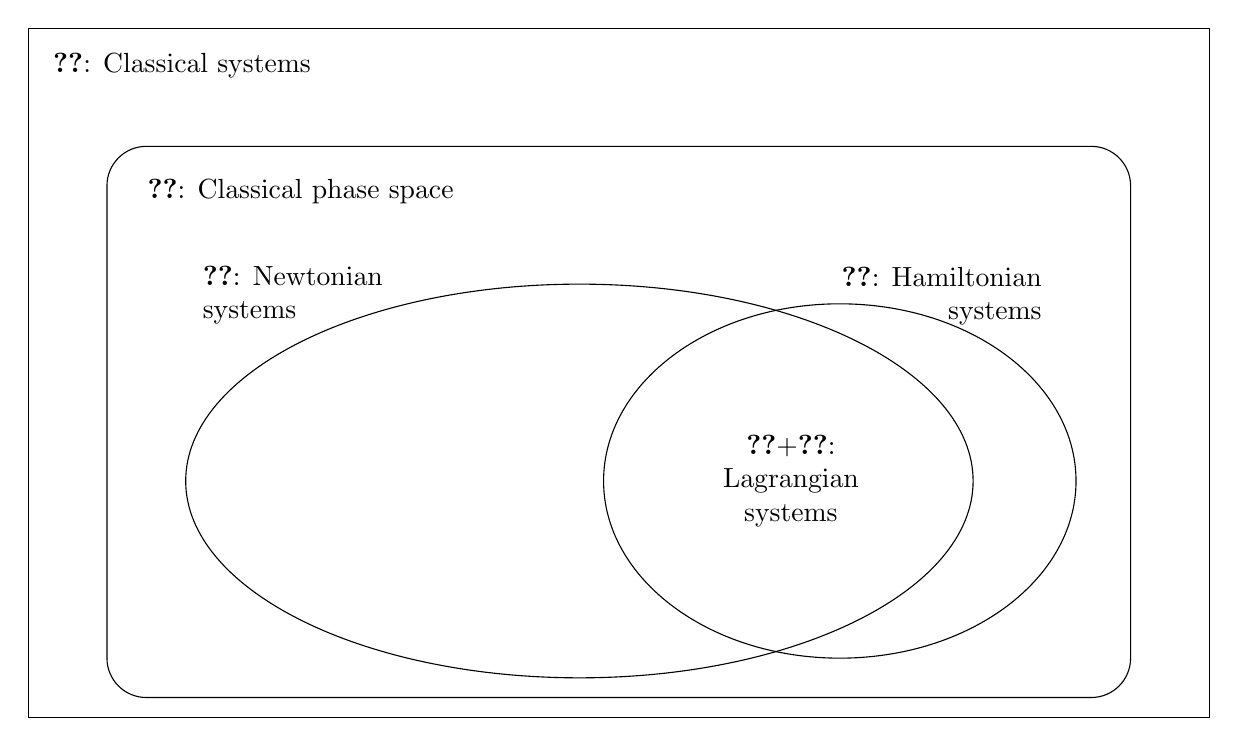
\begin{tikzpicture}
		\node[draw, minimum width=15cm, minimum height=8.75cm] (csx) {};
		\node[below right] at ([xshift=2mm,yshift=-2mm]csx.north west) {\ref{assum_infirr}: Classical systems};
		\node[draw, minimum width=13cm, minimum height=7cm, rounded corners=5mm, above] (inx) at ([yshift=0.25cm]csx.south) {};
		\node[below right] at ([xshift=4mm,yshift=-3mm]inx.north west) {\ref{assum_indep}: Classical phase space};
		
		\node[ellipse, minimum width=10cm, minimum height=5cm, draw, right] (ns) at ([xshift=1cm,yshift=-0.75cm]inx.west) {};
		\node [align=left, above] at ([xshift=-1mm,yshift=1mm]ns.north west) {\ref{assum_kineq}: Newtonian \\systems};
		
		\node[ellipse, minimum width=6cm, minimum height=4.5cm, draw] (hs) at ([xshift=-1.7cm]ns.east){};
		\node [align=right, above right] at ([xshift=-1mm, yshift=-4mm]hs.north) {\ref{assum_detrev}: Hamiltonian\\ systems};
		\node [align=center, right] at ([xshift=14
		mm]hs.west) {\ref{assum_kineq}+\ref{assum_detrev}: \\Lagrangian \\systems};
	\end{tikzpicture}
	\caption {Relationship between the constitutive assumptions and the different formulations of classical mechanics. All classical systems satisfy infinitesimal reducibility. The independence of DOF recovers classical phase space. An ideal gas, with state variables $[P \, V \, T]$ is an example of a classical system that does not satisfy IND. Another example is a systems with non-holonomic constraints. Newtonian system are fully characterized by spatial trajectories. Hamiltonian systems are characterized by deterministic and reversible dynamics. Lagrangian systems are characterized by both.}
\end{figure}
Let's step back and sum up all that we learned by applying the reverse physics approach to classical mechanics. If we start from scratch, the first assumption that we need to set is Infinitesimal Reducibility \ref{assum_infirr}. This tells us that the domain of classical physics is those objects that can be thought of as being made of arbitrarily small parts. For these objects, specifying the state of the whole system is equivalent to specifying the state of all the infinitesimal parts. In this context, a particle is an infinitesimal part, the limit of recursive reduction of parts into smaller parts. Mathematically, the assumption tells us that the state space of the particles is a differentiable manifold, together with a volume measure that defines the count of states for each region. The state space of a classical object is a distribution over such manifold.

We then add assumption \ref{assum_indep} that tells us that the system is decomposable into independent degrees of freedom. This means that not only are we able to count states over regions of state space, but we must be able to count configurations along each DOF. Moreover, the count of configurations over multiple DOFs must be the product of the count over each DOF. The only way to obtain this structure, so that the count is defined independently of the units used to describe states, is for the manifold to be even dimensional, and for any state variable $q^i$ that defines an independent unit, there is a conjugate state variable $p_i$ whose units are count of states over units of the corresponding $q^i$. This recovers the structure of classical phase space. Mathematically, this gives us the structure of a symplectic manifold, where the symplectic form $\omega_{ab}$ counts the configurations over the infinitesimal parallelogram defined by two vectors.

If we add assumption \ref{assum_detrev} that tells us that the evolution is deterministic and reversible, we recover Hamiltonian mechanics. For a system to be deterministic and reversible, in fact, we must map not only each initial state to one and only one final state, but we must map initial to final regions while preserving the state count. Moreover, the notion of independence must be preserved, and therefore the way configurations are counted over independent DOFs must also be preserved. Under these conditions, the displacement vector field, which tells us how states move in phase space, allows a potential $H$, which corresponds to the Hamiltonian. This can be generalized to the time-dependent case, which recovers relativistic features even without the notion of a metric tensor. Mathematically, the form $\omega_{ab}$ must be preserved, meaning deterministic and reversible evolution is a symplectomorphism. Each symplectomorphism can be characterized by a function $H$, the Hamiltonian.

If, instead, we add assumption \ref{assum_kineq} that tells us that the dynamics is recoverable from the kinematics, we recover Newtonian mechanics. If the dynamics is recoverable from the kinematics, the momentum must be a function of position and velocity. The units of position are the only independent units, and therefore define the units of momentum and also the transformation between densities over dynamic and kinematic variables. This forces the transformation between position and velocity to be linear. If no forces are present, we can find coordinates such that the linear transformation is simply a multiplication by a constant. That is, $p_i = m v^i$. These are the inertial frames in Cartesian coordinates and $m$ is the inertial mass. In this case, assumption \ref{assum_detrev} applies as well, and, since momentum is constant, the velocity is constant. If a force is present, this can be expressed in terms of position and velocity, recovering $F = m a$.

If we take both assumption \ref{assum_detrev} and \ref{assum_kineq}, Lagrangian mechanics is recovered. The action is the line integral over the potential $\theta_a$ of the form $\omega_{ab} = - \partial_a \wedge \theta_b$, and since the vector potential is unphysical, so is the action. The variation of the action is physical as, by Stokes' theorem, it will give the surface integral of $\omega_{ab}$, which is zero if and only if the path is always tangent to the direction of motion, which happens only if the path is an actual evolution of the system.

All the elements of classical mechanics, both physically and mathematically, can be understood just in terms of these assumptions and the concepts that they require.

%\begin{figure}[h]
%	\includegraphics[width=\columnwidth]{images/ClassicalDiagram.png}
%	\caption{TODO: redraw this diagram in tikz and update outdated text}\label{fig_classical_diagram}
%\end{figure}


\part{Physical Mathematics}

\begingroup
\pagestyle{plain}


\textbf{Physical mathematics} is an approach to the mathematical foundations of physics that seeks to construct mathematical structures strictly from axioms and definitions that can be rigorously justified from physical requirements. This is in contrast to current approaches typically followed in \textbf{mathematical physics}, which take tools developed within mathematics and apply them to physics or physics-inspired problems.

If our goal is to fully rederive physical theories from physical assumptions, we need to have a precise mapping between physical objects and mathematical ones. Understanding the axioms and definitions of the mathematical tools used in a physical theory, then, is not just ``mathematical detail'' of no concern to the physicist, but rather the precise stipulation of properties that certain physical objects must have under suitable, possibly simplifying, assumptions. In this sense, there is no ``correct'' structure in a mathematical sense, because the correct structure is the one suited to the physical problem at hand.

It should be clear that mathematicians are generally ill-equipped to determine whether mathematical structures are physically significant. As David Hilbert stated, ``Mathematics is a game played according to certain simple rules with meaningless marks on paper.'' Regarding mathematical axioms, Bertrand Russell claimed, ``It is essential not to discuss whether the first proposition is really true, and not to mention what the anything is, of which it is supposed to be true.'' Mathematics knows the rules of everything but the meaning of nothing. It is therefore unreasonable to expect that the foundations of mathematics, by themselves, can provide any foundation for physics.

In the same way that elaborate correct mathematical theories stem from minimal correct mathematical theories (not elaborate incorrect mathematical theories); that large living creatures grow from small living creatures (not large dead creatures); sophisticated physically meaningful theories come from simple physically meaningful theories (and not from sophisticated meaningless ones). Meaningfulness, like correctness or aliveness, is not something that can be imposed after the fact. Therefore the only way to develop physically meaningful mathematical structures is to develop them from scratch: we cannot simply take higher level mathematical objects and ``sprinkle meaning'', an interpretation, on top.

The goal of physical mathematics, then, is to find how to turn physical assumptions into precise mathematical requirements, such that we are guaranteed to know what exactly each mathematical object represents and under which physical conditions.

\subsection{A new standard for scientific rigor}

From the above discussion, it follows that the standard of rigor mathematicians have developed for their field is not sufficient for the purpose of physical mathematics. Mathematics only deals with formal systems, whose starting points are a set of definitions and rules that are taken as is. At that point, correctness of the premise cannot be established, only self-consistency. Therefore mathematics fails to deal with the most delicate and interesting parts of the foundations of physics: the physical assumptions and how they are encoded into the formal framework. We therefore need rules and standards for rigorously handling the informal parts of the framework and, since there are no guidelines for this, we set our own standard.

We call an \textbf{axiom} a proposition that brings new objects or new properties of established objects within the formal framework. A \textbf{definition}, instead, is a proposition that further characterizes objects and properties already present in the formalism. \textbf{An axiom or a definition is well posed only when it is clear what the objects represent physically and what aspects are captured mathematically.} Therefore each axiom and definition is composed of two parts. The first characterizes the objects and properties within the informal system, tells us what they represent physically. The second part, typically preceded by ``Formally'', characterizes the part that is captured by the formal system. Axioms and definitions are followed by a \textbf{justification} when it is necessary to explain why the elements in the informal system must be mapped into the formal system in the way proposed. Some definitions are purely formal and as such do not require justifications. As this argument spans both the formal and informal systems, this cannot be a mathematical proof in the modern sense. In particular, the justification for an axiom must argue why those objects must exist.

The above standard makes sure we have a perfect identification between formal and informal objects. All mathematical symbols correspond to physical objects and all the relevant physical concepts are captured by the math. All subsequent propositions and proofs, then, can be carried out in the formal system, where it is easier to check for consistency and correctness. However, all the proofs can, if needed, be translated into the informal language and given physical meaning.

\newpage
\endgroup

\chapter{Verifiable statements and experimental domains}

In this chapter we lay the foundations for our general mathematical theory of experimental science: a formalism that is broad enough to be applied to any area of scientific investigation. It is based on the idea of \textbf{verifiable statements}, assertions that can be experimentally shown to be true. Whether it is physics or chemistry, economics or psychology, medicine or biology, the goal is always to find some objective truth about the natural world that is supported by experimental data.

We group verifiable statements into \textbf{experimental domains} which represent the list of all possible verifiable answers to a particular scientific question. From those, we define \textbf{theoretical domains} which add those statements that, though not directly verifiable, are associated to an experimental test with no guarantee of termination. Within each theoretical domain, we find those particular statements that, if true, imply the truthfulness or falsehood of all other statements. We call these the \textbf{possibilities} of the domain as they identify the complete descriptions that are admissible. To answer a scientific question, then, is to find which possibility is consistent with experimental data: the one that correctly predicts the result of all experimental tests.

We'll see how the above organization always exists on any given set of verifiable statements. That is, it is a fundamental structure for all sciences. We'll also see that these concepts are deeply intertwined with fundamental mathematical tools: experimental domains map to topologies while theoretical domains map to $\sigma$-algebras. These two core mathematical structures provide the foundation for differential geometry, Lie algebras, measure theory, probability theory and other mathematical branches that are heavily used in physics and other sciences.

As a consequence of this connection, we can build a more precise, intuitive and insightful understanding of what these mathematical structures are meant to represent in the scientific world. It also reveals why these mathematical tools are so pervasive and successful in science.

\section{Statements}

Statements, like \statement{the mass of the electron is $511 \pm 0.5$ keV} or \statement{that animal is a cat}, will be the cornerstone of our general mathematical theory of experimental science. In this section we will outline the basic definitions that allow us to combine statements into other statements (e.g. \statement{that animal is black} and \statement{that animal is a cat} gives \statement{that animal is a black cat}) and to compare their content (e.g. \statement{the mass of the electron is $511 \pm 0.5$ keV} and \statement{the mass of the electron is $0.511 \pm 0.0005$ MeV} are equivalent).

We will start from a somewhat different starting point than what is customary in order to address a few issues. The first is that we need to develop a formal framework to handle the relationship of statements that are not themselves formally defined.\footnote{This is the main reason we cannot simply use the tools of mathematical logic.} The second issue is that the truth values in our context are in general found experimentally, not through deduction. The role of the logic framework is to keep track of the consistency between the possible hypothetical cases. That is, we need relationships that capture the idea of causal relationship, that one is true because the other is true, and not merely by coincidence.\footnote{In contrast, in standard logic ``the moon is a satellite of earth" implies ``5 is prime".} We remind the reader that the mathematical sections, highlighted with a green bar on the side, can be skipped without loss of conceptual understanding in case one is not interested in all the details. 

As a starting point, we need to define what science is: the systematic study of the physical world through observation and experimentation. We therefore introduce the principle of scientific objectivity that will guide us throughout this work. This states that science is universal, non-contradictory and evidence based.

\begin{mathSection}
	\textbf{Principle of scientific objectivity}.
		Science is universal, non-contradictory and evidence based.
\end{mathSection}

Consider assertions like \statement{jazz is marvelous} or \statement{green and red go well together}. These are not objective: there is no agreed upon definition or procedure for what constitutes marvelous music or good color combination. Because of their nature, they can't be the subject of scientific inquiry. This does not mean that marvelous music or good color combinations do not exist or are not worth studying.\footnote{In fact, one can argue that most of the things that make life worth living (e.g. love, friendship, arts, purpose and so on) defy objective characterization and, therefore, that science gives us certain truth about trifling matters.} What the principle tells us is simply that if we choose to do science, we are limiting ourselves to those assertions that are either true or false (i.e.~non-contradictory) for everybody (i.e.~universal): assertions that have a single truth value. We call these assertions statements: they are the basic building blocks of a scientific description as only these can be studied scientifically.

Logical consistency, though, is not just a property of individual statements. Consider the following two sentences:
\begin{description}
	\item \statement{the next sentence is true}
	\item \statement{the previous sentence is false}
\end{description}
Each assertion, by itself, would be fine but their combination makes it impossible to assign truth values to both in a way that is logically consistent. For this reason we group statements into logical contexts, sets of statements for which it is possible to assign truth values to all in a way that is logically consistent.

\begin{mathSection}
\begin{defn}
	The \textbf{Boolean domain} is the set $\Bool = \{\FALSE, \TRUE\}$ of all possible truth values.
\end{defn}


\begin{axiom}[Axiom of context]\label{ax_statement}
	A \textbf{statement} $\stmt$ is an assertion that is either true or false. A \textbf{logical context} $\logCtx$ is the collection of all those statements that share a common semantics and have, therefore, well defined logical relationships. Formally, a logical context $\logCtx$ is a collection of elements called statements upon which is defined a function $\truth: \logCtx \to \Bool$.
\end{axiom}

\begin{justification}
	As science is universal and non-contradictory, it must deal with assertions that have clear meaning, well-defined logical relationships and are associated with a unique truth value. A priori, we only assume these objects exist, simply because we cannot proceed if we do not. A posteriori, we see that a particular set of statements works in practice, which shows that science could indeed be done with those statements. We are therefore justified to assume the existence of sets of assertions that have the aforementioned properties. We call a logical context such a group of assertions and we represent it formally as a set $\logCtx$. We call statement each assertion within a logical context and represent it formally with an element $\stmt$. We say $\stmt \in \logCtx$ if the statement $\stmt$ belongs to the logical context $\logCtx$.
	
	Given a context, we are also justified to assume the existence of a function $\truth : \logCtx \to \Bool$ such that $\truth(\stmt) = \TRUE$ for all $\stmt \in \logCtx$ that are true for everybody and $\truth(\stmt) = \FALSE$ for all $\stmt \in \logCtx$ that are false for everybody. In fact, note that no $\stmt \in \logCtx$ can be both true and false for everybody as it would be contradictory. Note that no $\stmt \in \logCtx$ can be both true for some and false for others as it would not be universal. Note that no $\stmt \in \logCtx$ can be neither true nor false for everybody. Suppose it were. Then its truth can never be, even potentially, settled with experimental evidence. Therefore either $\truth(\stmt) = \TRUE$ or $\truth(\stmt) = \FALSE$ for all $\stmt \in \logCtx$.

	Note that the statement is the concept asserted, not the words used to express the concept. A sentence in a particular language is neither necessary nor sufficient to define a statement. Consider the English language and take the sentence \statement{Snoopy is a dog}. The truth will depend on whether or not a fictional character qualifies as a dog. The sentence, by itself, is not enough to determine the truth value. Conversely, take the idea that a particular animal is a dog. We can express the concept in Italian as \statement{quell'animale \`e un cane} without using an English sentence. Therefore English sentences are neither necessary nor sufficient to express a statement. This will be true of any other language. Therefore, the basic notion of statement is considered prime, 
	independent of its expression. Moreover, all statements are considered equally prime.
	
	Also note that logical consistency is not a property of an individual statement but rather of a set of statements. Consider the two statements: \statement{the next sentence is true} and \statement{the previous sentence is false}. The two statements together are not logically consistent as assuming one to be true leads to a proof for it to be false and vice-versa. If we changed the latter statement to \statement{the previous sentence is true} then both statements would be true and logically consistent. Therefore logical consistency is defined on the logical context, and each statement has to be defined as belonging to a context.
	
	Finally, note that the existence of a truth function on the context imposes logical consistency on the logical context without worrying about the details of how this is achieved.
	
\end{justification}

\end{mathSection}

The idea of statements has their origin in the philosophical tradition of classical logic, \statement{Socrates is a man} being a classic example. Any language can be used to form them, formal or natural, as indeed any language is used in practice. This means we are not going to care what particular syntax (i.e.~symbols and grammar rules) is used.\footnote{In general, statements in this context are not necessarily well formed formulas, predicates or similar concepts in the context of mathematical or propositional logic. Scientific investigation in the broad sense of learning from experimentation predates math and formal languages: information about agriculture, astronomy, metallurgy, botany and the like were collected and used even before the written word. Moreover, cognitive scientists have shown that children start using deliberate experimentation at a very young age to understand the world around them, even before their speech is fully developed. Ultimately, that knowledge is encoded in the language of electrical and biochemical signals. Formal languages are indeed extremely helpful in that they allow us to be more precise and to better keep track of possible inconsistencies, but ultimately one always needs natural language to give meaning and context to the mathematical symbols.} In fact, even a grammatically incorrect statement is fine as long as the intent is clear. On the other hand, we are going to care about the semantics of the statements (i.e.~their content and meaning). Therefore we will consider \statement{Socrates is a man} and \statement{Socrate \`{e} un uomo} to be the same statement because they provide the same assertion but in different languages.

Moreover, when we say \statement{Socrates is a man} it has to be clear who is Socrates and what a man is. If it weren't, we would have no idea what to experimentally test and how. This is also important because the mere content of a set of statements puts constraints on what can be found to be true or false. Consider the statement \statement{that cat is a swan}. There is nothing to experimentally test here: based on the definitions of cat and swan we know the statement can never be true, no matter what particular cat we are considering. The statement provides no new information. Consider, instead, the statements \statement{that animal is a mammal} and \statement{that animal is a bird}. Based on the content, each of the statements can be found true or false separately, but they can't be found true together simply by how mammals and birds are defined.

We want each logical context to keep track not only of the truth value of each statement, but also of which truth combinations are possible merely because of the content. Given a logical context $\logCtx$ we will call an assignment for $\logCtx$ a map $a : \logCtx \to \Bool$ that for each statement gives a truth value. For example, consider the following table:
\begin{center}
	\begin{tabular}{c|c|c|c}
		\statement{that animal is a cat} & \statement{that animal is a mammal} & \statement{that animal is a bird} & ... \\
		\hline
		T & T & T & ... \\
		T & T & F & ... \\
		F & F & T & ... \\
		F & T & F & ... \\
	\end{tabular}
\end{center}
Each line represents an assignment for all statements, each represented by a column. The set of all assignments is the set of all functions from $\logCtx$ to $\Bool$, which in set theory notation is $\Bool^\logCtx$, and corresponds to all possible permutations. Some assignments, like the one in the first line, are not consistent with the content of the statements. We will call possible the ones that are allowed and impossible the ones that aren't. Naturally, the truth must be one of the possible assignments. As the context itself needs to tell us which assignments are possible, we can imagine it comes equipped with the set $\pAss \subseteq \Bool^\logCtx$ of all possible assignments for that context.\footnote{In the same way that we do not try to capture how statements are constructed, we are not going to capture how logical consistency is established. We just assume a mechanism is available and therefore one can check whether an assignment is possible or not.}

Some statements may be allowed to either be true or false while others may only be allowed one option. We will call certainty a statement that can only be true, like \statement{that cat is an animal}. We will call impossibility a statement that can only be false, like \statement{that cat is a swan}. We will call a contingent statement one that can be either true or false as its truth is contingent on the assignment, like \statement{that animal is a cat}.

Note that the semantics, the meaning of the statements, plays an important role in defining the possible assignments but, in general, does not define the truth values.\footnote{In other formalisms the semantics is said to define the truth values, not in ours.} For example, even if the meaning of \statement{the next race is going to be won by Secretariat} is clear, and so is its logical relationship to \statement{the next race is going to be lost by Secretariat}, we may be none the wiser about its truthfulness. 

\begin{mathSection}
\begin{defn}
	Given a set of statements, an \textbf{assignment} associates a truth value with each statement. Formally, an assignment for a logical context $\logCtx$ is a map $a : \logCtx \to \Bool$, an element of $\Bool^\logCtx$. An assignment for a set of statements $S \subseteq \logCtx$ is a map $a : S \to \Bool$ while an assignment for a statement $\stmt \in \logCtx$ is a truth value $t \in \Bool$.
\end{defn}

\begin{justification}
	Given that an assignment for a set $S \subseteq \logCtx$ associates a truth value to each statement, it is identified by a map $a : S \to \Bool$. The assignment for a single statement is given by a single truth value $t \in \Bool$.
\end{justification}

\begin{axiom}[Axiom of possibility]\label{ax_possible_assignemetns}
	A \textbf{possible assignment} for a logical context $\logCtx$ is a map $a : \logCtx \to \Bool$ that assigns a truth value to each statement in a way consistent with the content of the statements. Formally, each logical context comes equipped with a set $\pAss \subseteq \Bool^{\logCtx}$ such that $\truth \in \pAss$. A map $a : \logCtx \to \Bool$ is a possible assignment for $\logCtx$ if $a \in \pAss$.
\end{axiom}

\begin{justification}
	The meaning associated to each statement in the context may prevent some assignments from being logically consistent. Consider, for example, the statements \statement{that animal is a cat} and \statement{that animal is a dog}. Given that an animal cannot be both a cat and a dog, an assignment that associated true to both statements would not be logically consistent. Given that the context must give clear meaning to all statements, it must be able to clarify whether an assignment $a \in \Bool^{\logCtx}$ is consistent with the meaning of all statements. We call these possible assignments.
	
	For each logical context, then, we are justified to assume the existence of a set $\pAss \subseteq \Bool^{\logCtx}$ such that $a \in \pAss$ if and only if $a$ is a possible assignment.
\end{justification}

\begin{defn}
	Let $S \subseteq \logCtx$ be a set of statements. Then $a : S \to \Bool$ is a possible assignment for $S$ if there exists $\bar{a} \in \pAss$ such that $\bar{a}(\stmt) = a(\stmt)$ for all $\stmt \in S$. Let $\stmt \in \logCtx$ be a statement. Then $t \in \Bool$ is a possible assignment for $\stmt$ if there exists $\bar{a} \in \pAss$ such that $\bar{a}(\stmt) = t$.
\end{defn}

\begin{justification}
	Let $S \in \logCtx$ be a set of statements. If $a : S \to \Bool$ is a possible assignment then there must be a way to assign the remaining statements in the domain in a way that is logically consistent. Therefore there must be an $\bar{a} \in \pAss$ such that $\bar{a}(\stmt) = a(\stmt)$ for all $\stmt \in S$. Similarly, $t \in \Bool$ is a possible assignment for $\stmt$ if there exists $\bar{a} \in \pAss$ such that $\bar{a}(\stmt) = t$. This justifies the definition.
\end{justification}

\begin{defn}
	Statements are categorized based on their possible assignments.
	
	\begin{itemize}
		\item A certain statement, or \textbf{certainty}, is a statement $\certainty$ that must be true simply because of its content. Formally, $a(\certainty) = \TRUE$ for all possible assignments $a \in \pAss$.
		\item An impossible statement, or \textbf{impossibility}, is a statement $\impossibility$ that must be false simply because of its content. Formally, $a(\impossibility) = \FALSE$ for all possible assignments $a \in \pAss$.
		\item A statement is \textbf{contingent} if it is neither certain nor impossible.
	\end{itemize}
	
\end{defn}

\begin{justification}
	Since a certainty must be true, no possible assignment can assign it to be false. Therefore $a(\certainty) = \TRUE$ for all $a \in \pAss$. Similarly, an impossibility must be false and no possible assignment can assign it to be true. Therefore $a(\impossibility) = \FALSE$ for all $a \in \pAss$. This justifies the definitions.
\end{justification}

\begin{coro}
	A statement $\stmt \in \logCtx$ can only be exactly one of the following: impossible, contingent, certain.
\end{coro}

\begin{proof}
	Let $\stmt \in \logCtx$ be a statement. If it is contingent, by definition, it is neither certain nor impossible. If it is not contingent, it is either certain or impossible. If $\stmt$ is certain, then $a(\stmt) = \TRUE$ for all possible assignments $a \in \pAss$. This means $a(\stmt) \neq \FALSE$ for all possible assignments $a \in \pAss$ and therefore $\stmt$ is not impossible. If $\stmt$ is impossible, then $a(\stmt) = \FALSE$ for all possible assignments $a \in \pAss$. This means $a(\stmt) \neq \TRUE$ for all possible assignments $a \in \pAss$ and therefore $\stmt$ is not certain.
\end{proof}

\end{mathSection}

Next we want to keep track of statements whose truth depends on the truth of other statements. Consider \statement{that animal is a cat} and \statement{that animal is not a cat}: if the first one is true then the second is false and vice-versa. In this sense, the second statement depends on the first. Therefore, in general, a statement depends on other statements if its truth is determined by the truth values of the other statements in every possible assignment.

Since statements are intangible, there are no limits to the number of arguments one statement may depend on. For example, consider the statement \statement{the mass of the electron is $511 \pm 0.5$ keV} and the set of all the statements of the form \statement{the mass of the electron is exactly $x$ keV} with $510.5 < x < 511.5$. If any of the latter is true then the original statement is true as well. Given that $x$ is a real number, that is uncountably many statements so the original statement can be seen as a function of uncountably many statements. Therefore we will assume we can always create a statement that arbitrarily depends on an arbitrary set of statements.

\begin{mathSection}
	\begin{defn}\label{def_dependence}
	Let $\bar{\stmt} \in \logCtx$ be a statement and $S \subseteq \logCtx$ be a set of statements. Then $\bar{\stmt}$ \textbf{depends on} $S$ (or it is a function of $S$)  if we can find an $f_\Bool : \Bool^S \to \Bool$ such that
	$$a(\bar{\stmt}) = f_\Bool (\{a(\stmt)\}_{\stmt \in S})$$
	for every possible assignment $a \in \pAss$. We say $\bar{s}$ depends on $S$ \textbf{through} $f_\Bool$. The relationship is illustrated by the following diagram:
\end{defn}

\begin{center}
	\begin{tabular}{  c  c  c | c |  c | c  c  c  c  }
		\multicolumn{2}{c}{} & \multicolumn{4}{c}{$\overbrace{\rule{2.2cm}{0pt}}^{S \subseteq \logCtx}$} \\
		
		{  } & {  }  & $\stmt_1$ & $\stmt_2$ & $\stmt_3$ & ... & {  } & $\bar{\stmt}$ &    \\
		\cline{3-6}
		\cline{8-8}
		\multirow{4}{0.5cm}{$\pAss \left\{ \parbox[][2cm]{0cm}{} \right.$} & $a_1$ & T & T & F & ... & \multirow{2}*{$f_\Bool$}  & T & $a_1(\bar{\stmt})=f_\Bool$({T,T,F}) \\
		
		& $a_2$ &	T & F & T & ... & \multirow{2}*{$\overrightarrow{\rule{2.2cm}{0pt}}$} & T & $a_2(\bar{\stmt})=f_\Bool$({T,F,T})  \\
		
		& $a_3$ &	T & F & F & ... & \multirow{2}*{$\stmt_1$ AND ($\stmt_2$ OR $\stmt_3$) } & F & $a_3(\bar{\stmt})=f_\Bool$({T,F,F})  \\
		
		& $...$ &	... & ... & ... & ... & {   } & ... & $f_\Bool$({...,...,...})  \\
	\end{tabular}
\end{center}

	\begin{axiom}[Axiom of closure]\label{ax_functions_of_statement}
		We can always find a statement whose truth value arbitrarily depends on an arbitrary set of statements. Formally, let $S \subseteq \logCtx$ be a set of statements and $f_{\Bool} : \Bool^S \to \Bool$ an arbitrary function from an assignment of $S$ to a truth value. Then we can always find a statement $\bar{\stmt} \in \logCtx$ that depends on $S$ through $f_{\Bool}$.
	\end{axiom}
\begin{justification}
	Let $S \subseteq \logCtx$ be a set of statements and let $f_{\Bool} : \Bool^S \to \Bool$ be an arbitrary function. Consider the statement $\bar{\stmt}=$\statement{this statement is true if and only if the function $f_{\Bool}$ applied to the truth values of $S$ is true}. The meaning of $\bar{\stmt}$ is determined by the meaning of the statements in $S$, and, for every possible assignment $a \in \pAss$, $\bar{\stmt}$ is assigned the truth value $f_\Bool (\{a(\stmt)\}_{\stmt \in S})$ that is the same for everybody. Therefore $\bar{\stmt}$ shares a common semantics with the statements in $S$, and has a well-defined logical relationship with all other statements in $\logCtx$. Given that a context, by definition, contains all such statements, we are justified to assume $\bar{\stmt} \in \logCtx$.
\end{justification}

\begin{remark}
	If it can be proven that the closure can always be performed, that proof, together with the definition of closure, would replace the axiom. This would be preferable but, given that the closure would be on possibly infinite elements, this is a delicate problem that we have not addressed yet.
\end{remark}

\begin{coro}
	Functions on truth values induce functions on statements. Formally, let $I$ be an index set and $f_\Bool : \Bool^I \to \Bool$ be a function. There exists a function $f : \logCtx^I \to \logCtx$ such that
	$$a(f(\{\stmt_i\}_{i \in I})) = f_{\Bool}(\{a(\stmt_i)\}_{i \in I})$$
	for every indexed set $\{\stmt_i\}_{i \in I} \subseteq \logCtx$ and possible assignment $a \in \pAss$.
\end{coro}
\begin{proof}
	Given $I$ and $f_\Bool : \Bool^I \to \Bool$ we can construct $f : \logCtx^I \to \logCtx$ as follows. Given an indexed set $\{\stmt_i\}_{i \in I} \in \logCtx^I$, let $S \subseteq \logCtx$ be the set of elements in the indexed set and define $\bar{f}_\Bool : \Bool^S \to \Bool$ such that $\bar{f}_\Bool(\{a(\stmt)\}_{\stmt \in S}) = f_{\Bool}(\{a(\stmt_i)\}_{i \in I})$. Then by axiom \ref{ax_functions_of_statement} we can find a statement $\bar{\stmt}$ that depends on $S$ through $\bar{f}_\Bool$ and we can set $f(\{\stmt_i\}_{i \in I}) = \bar{\stmt}$. We have $a(f(\{\stmt_i\}_{i \in I})) = f_{\Bool}(\{a(\stmt_i)\}_{i \in I})$ for all indexed sets and for all possible assignments.
\end{proof}
\end{mathSection}

To better characterize truth functions, we borrow ideas and definitions from Boolean algebra which is the branch of algebra that operates on truth values. Boolean algebra is fundamental in logic and computer science, since every digital circuit ultimately is implemented on two-state systems (e.g. high/low voltage, up/down magnetization).  The most fundamental elements in that algebra are the following three simple operations: negation (i.e.~logical NOT), conjunction (i.e.~logical AND) and disjunction (i.e.~logical OR).

Suppose $\stmt_1$ = \emph{``the sauce is sweet"} and $\stmt_2$ = \emph{``the sauce is sour"}. We can apply the three operations to make this table:

\begin{table}[h]
	\centering
	\begin{tabular}{p{0.2\textwidth} p{0.1\textwidth} p{0.1\textwidth} p{0.5\textwidth}}
		Operator & Gate & Symbol & Example \\ 
		\hline 
		Negation & NOT & $\NOT \stmt_1$ &  \emph{``the sauce is not sweet"} \\ 
		Conjunction & AND & $\stmt_1 \AND \stmt_2$ & \emph{``the sauce is sweet and sour"} \\ 
		Disjunction & OR & $\stmt_1 \OR \stmt_2$ & \emph{``the sauce is at least sweet or sour"}
	\end{tabular} 
	\caption{Boolean operations on statements.}
\end{table}

Most languages, natural or symbolic, typically already provide similar operations, as the examples show. Technically, though, we should consider the ones defined here as meta-operations that are defined outside the language of the statements. For example, \statement{x is the position of a ball}$\AND$\statement{$\,\frac{d^2 x}{dt^2} = - g$} stitches together an English statement with a calculus statement into a new statement that is neither. This kind of mix should be allowed as it does happen in practice.

\begin{mathSection}
	\begin{defn}
		The \textbf{negation or logical NOT} is the function $\NOT : \Bool \to \Bool$ that takes a truth value and returns its opposite. That is: $\NOT \TRUE = \FALSE$ and $\NOT \FALSE = \TRUE$. We also call negation $\NOT: \logCtx \to \logCtx$ the related function on statements.
	\end{defn}
	
	\begin{defn}
		The \textbf{conjunction or logical AND} is the function $\AND : \Bool \times \Bool \to \Bool$ that returns $\TRUE$ only if all the arguments are $\TRUE$. That is: $\TRUE \AND \TRUE = \TRUE$ and $\TRUE \AND \FALSE =\FALSE \AND \TRUE =\FALSE \AND \FALSE = \FALSE$. We also call conjunction $\AND : \logCtx \times \logCtx \to \logCtx$ the related function on statements.
	\end{defn}
	
	\begin{defn}
		The \textbf{disjunction or logical OR} is the function $\OR : \Bool \times \Bool \to \Bool$ that returns $\FALSE$ only if all the arguments are $\FALSE$. That is: $\FALSE \OR \FALSE = \FALSE$ and $\TRUE \OR \FALSE =\FALSE \OR \TRUE =\TRUE \OR \TRUE = \TRUE$.  We also call disjunction $\OR : \logCtx \times \logCtx \to \logCtx$ the related function on statements.
	\end{defn}

	\begin{prop}
	A logical context $\logCtx$ is closed under negation, arbitrary conjunction and arbitrary disjunction.
\end{prop}
\begin{proof}
	Negation, arbitrary conjunction and arbitrary disjunction are particular truth functions. Their output always exists by axiom \eqref{ax_functions_of_statement}.
\end{proof}\end{mathSection}

Now we have all the elements to define when two statements have the same logical content. Consider the two statements \statement{that animal is a bird} and \statement{that animal has feathers}: since all birds and only birds have feathers they give us the same information. Consider \statement{the mass of the electron is $511 \pm 0.5$ keV} and \statement{the mass of the electron is $0.511 \pm 0.0005$ MeV}: they represent the same measurement but in different units. So, how can we express the fact that two statements $\stmt_1$ and $\stmt_2$ give us the same information? The idea is that they can never be assigned opposite truth values. If we assigned true to the first, then the second must be true as well. If we assigned false to the first, then the second must be false.\footnote{This technique allows us to do something analogous to model theory. Two statements are equivalent if their truth is equal for all consistent truth assignments, which in our framework play the part of the models of model theory. But in our context the assignments are only hypothetical: there isn't a model in which \statement{this is a cat} and another in which \statement{this is a dog}. There is only one truth value, the one we find experimentally.}

\begin{mathSection}

\begin{defn}
	Two statements $\stmt_1$ and $\stmt_2$ are \textbf{equivalent} $\stmt_1 \equiv \stmt_2$ if they must be equally true or false simply because of their content. Formally, $\stmt_1 \equiv \stmt_2$ if and only if $a(\stmt_1)=a(\stmt_2)$ for all possible assignments $a \in \pAss$.
\end{defn}

\begin{justification}
	If two statements must be equally true or false simply because of their content, then their value must be the same in all possible assignments, which justifies the definition.
\end{justification}

%TODO: note that the definitions of NOT, AND, OR on statements are problematic because the function induced from the function on truth value is not unique. It is unique, however, on the equivalence class of statements. We should be able to move the definition of equivalence before the axiom of closure, so that everything after is on the equivalence classes.

\end{mathSection}

Again, we want to stress that this notion of equivalence is not based on the truth value (i.e.~whether the statements happen to be both true or false) or on whether they are the same statement (i.e.~whether they assert the same thing): it is based on the possible assignment (i.e.~whether there exists a possible assignment in which the two statements have a different truth value) and therefore on the content of the statements. We sum up the difference in the following table.


\begin{table}[h]
	\centering
	%	\begin{tabular}{p{0.2\textwidth} p{0.1\textwidth} p{0.1\textwidth} p{0.5\textwidth}}
	\begin{tabular}{p{0.10\textwidth} c p{0.2\textwidth} p{0.25\textwidth} p{0.10\textwidth}}
		& & & & Also \\ 
		Relationship & Symbol & First statement & Second statement & known as \\ 
		\hline 
		Statement & $\stmt_1 = \stmt_2$ & \statement{Swans are birds} & \statement{I cigni sono uccelli} & Semantic \\ 
		equality & & & & equivalence \\ 
		Statement & $\stmt_1 \equiv \stmt_2$ & \statement{Swans are birds}  & \statement{Swans have feathers} & Logical \\ 
		equivalence & & & & equivalence \\ 
		Truth & $\truth(\stmt_1) = \truth(\stmt_2)$ & \statement{Swans are birds}  & \statement{The earth is round} & Material \\ 
		equality & & & & equivalence \\ 
	\end{tabular}
	\caption{Different types of statement relationships.}
\end{table}

Note that the relationships in the table are ordered by strength: if two statements are equal, they are also equivalent; if two statements are equivalent, they have equal truth. The reverse is not true in general: two statements with equal truth may not be equivalent; two equivalent statements may not be equal.

Intuitively, statement equivalence answers the question: do these two statements carry the same information? Is experimentally testing the first the same as experimentally testing the second? If that's the case, they are essentially equivalent to us. So much so, that from now on we will implicitly assume two different statements to be inequivalent.\footnote{Technically, when we'll say that $\stmt$ is a statement we actually mean $\stmt$ is an equivalence class of statements. We are not going to be explicit about the distinction, though, as we feel it simply distracts without adding greater clarity. We'll let the context determine what is meant.}

There are a number of useful properties that statement equivalence satisfies.

\begin{mathSection}

\begin{coro}
	All certainties are equivalent. All impossibilities are equivalent.
\end{coro}
\begin{proof}
	Let $\certainty_1, \certainty_2 \in \logCtx$ be two certainties. Then for every possible assignment $a \in \pAss$ we have $a(\certainty_1) = \TRUE = a(\certainty_2)$ and therefore $\certainty_1 \equiv \certainty_2$ by definition.
	
	Let $\impossibility_1, \impossibility_2 \in \logCtx$ be two impossibilities. Then for every possible assignment $a \in \pAss$ we have $a(\impossibility_1) = \FALSE = a(\impossibility_2)$ and therefore $\impossibility_1 \equiv \impossibility_2$ by definition.
\end{proof}

\begin{coro}
	Two statements $\stmt_1$ and $\stmt_2$ are equivalent if and only if $(\stmt_1 \AND \stmt_2) \OR (\NOT\stmt_1 \AND \NOT\stmt_2) \equiv \certainty$.
\end{coro}
\begin{proof}
	Let $a \in \pAss$ and $\stmt = ( \stmt_1 \AND \stmt_2) \OR (\NOT\stmt_1 \AND \NOT\stmt_2)$. We have $a(\stmt) = (a(\stmt_1) \AND a(\stmt_2)) \OR (\NOT a(\stmt_1) \AND \NOT a(\stmt_2))$. We have the following truth table
	\begin{center}
	\begin{tabular}{c|c|c}
		$\stmt_1$ & $\stmt_2$ & $\stmt$\\
		\hline
		T & T & T \\
		T & F & F \\
		F & T & F \\
		F & F & T\\
	\end{tabular}
	\end{center}
	Note that the assignments for which $a(\stmt_1) = a(\stmt_2)$ are exactly the assignments for which $a(\stmt) = \TRUE$. Therefore $\stmt_1 \equiv \stmt_2$ if and only if $\stmt$ is a certainty.
\end{proof}

\begin{coro}
	Statement equivalence satisfies the following properties:
	\begin{itemize}
		\item reflexivity: $\stmt \equiv \stmt$
		\item symmetry: if $\stmt_1 \equiv \stmt_2$ then $\stmt_2 \equiv \stmt_1$
		\item transitivity: if $\stmt_1 \equiv \stmt_2$ and $\stmt_2 \equiv \stmt_3$ then $\stmt_1 \equiv \stmt_3$
	\end{itemize}
	and is therefore an \textbf{equivalence relationship}.
\end{coro}
\begin{proof}
	Statement equivalence is defined in terms of truth equality within all possible assignments and will inherit reflexivity, symmetry and transitivity from it.
\end{proof}

\begin{coro}\label{boolean_properties}
	A logical context $\logCtx$ satisfies the following properties:
	\begin{itemize}
		\item associativity: $a \OR (b \OR c) \equiv (a \OR b) \OR c$, $a \AND (b \AND c) \equiv (a \AND b) \AND c$
		\item commutativity: $a \OR b \equiv b \OR a$, $a \AND b \equiv b \AND a$
		\item absorption: $a \OR (a \AND b) \equiv a$, $a \AND (a \OR b) \equiv a$
		\item identity: $a \OR \impossibility \equiv a
		$, $a \AND \certainty \equiv a$
		\item distributivity: $a \OR (b \AND c) \equiv (a \OR b) \AND (a \OR c)$, $a \AND (b \OR c) \equiv (a \AND b) \OR (a \AND c)$
		\item complements: $a \OR \NOT a \equiv \certainty$, $a \AND \NOT a \equiv \impossibility$
		\item De Morgan: $\NOT a \OR \NOT b \equiv \NOT (a \AND b)$, $\NOT a \AND \NOT b \equiv \NOT (a \OR b)$
	\end{itemize}
	Therefore $\logCtx$ is a \textbf{Boolean algebra} by definition.
\end{coro}
\begin{proof}
	The left and right expressions for each equivalence correspond to the same truth function applied to the same statements. Therefore, the left side is true if and only if the right side is true and they are therefore equivalent by definition.
\end{proof}
\end{mathSection}

These operations and properties define the \textbf{algebra of statements}. While we started from a slightly different premise, the relationships we found are the logical identities of classical logic. These are exactly what we need to make sure the truth values of all our statements are consistent.

Equivalence is not the only semantic relationship that we want to capture. Consider the contents of the following:
\begin{description}
	\item $\stmt_1=$\statement{that animal is a cat}
	\item $\stmt_2=$\statement{that animal is a mammal}
	\item $\stmt_3=$\statement{that animal is a dog}
	\item $\stmt_4=$\statement{that animal is black}
\end{description}
The second will be true whenever the first is true. In this case we say the first statement is narrower than the second ($\stmt_1$ $\narrower$ $\stmt_2$) because \statement{that animal is a cat} is more specific than \statement{that animal is a mammal}. The third will be false whenever the first is true. In this case we say that they are incompatible ($\stmt_1$ $\ncomp$ $\stmt_3$) because \statement{that animal is a dog} and \statement{that animal is a cat} can never be true at the same time. The fourth will be true or false regardless of whether the first is true. In this case we say that they are independent ($\stmt_1$ $\indep$ $\stmt_4$) because knowing whether \statement{that animal is a cat} tells us nothing about whether \statement{that animal is black}. As for equivalence, we can define these relationships upon the previous definitions.

\begin{mathSection}

\begin{defn}\label{def_statement_narrowness_and_compatibility}
	Given two statements $\stmt_1$ and $\stmt_2$, we say that:
	\begin{itemize}
		\item $\stmt_1$ \textbf{is narrower than} $\stmt_2$ (noted $\stmt_1 \narrower \stmt_2$) if $\stmt_2$ is true whenever $\stmt_1$ is true simply because of their content. That is, for all $a \in \pAss$ if $a(\stmt_1)=\TRUE$ then $a(\stmt_2)=\TRUE$.
		\item $\stmt_1$ \textbf{is broader than} $\stmt_2$ (noted $\stmt_1 \broader \stmt_2$) if $\stmt_2 \narrower \stmt_1$.
		\item $\stmt_1$ \textbf{is compatible to} $\stmt_2$ (noted $\stmt_1 \comp \stmt_2$) if their content allows them to be true at the same time. That is, there exists $a \in \pAss$ such that $a(\stmt_1)=a(\stmt_2)=\TRUE$.
	\end{itemize}
	The negation of these properties will be noted by $\nnarrower$, $\nbroader$ , $\ncomp$ respectively.
\end{defn}
\begin{defn}\label{def_independent_statements}
	The elements of a set of statements $S \subseteq \logCtx$ are said to be \textbf{independent} (noted $\stmt_1 \indep \stmt_2$ for a set of two) if the assignment of any subset of statements does not depend on the assignment of the others. That is, a set of statements $S \subseteq \logCtx$ is independent if given a family  $\{t_{\stmt}\}_{\stmt \in S}$ such that each $t_{\stmt} \in \Bool$ is a possible assignment for the respective $\stmt$ we can always find $a \in \pAss$ such that $a(\stmt) = t_{\stmt}$ for all $\stmt \in S$.
\end{defn}

\begin{prop}\label{prop_narrowness_properties}
	The above operations obey the following relationships:
	\begin{enumerate}[label=(\roman*)]
		\item 	$\stmt_1 \narrower \stmt_2$ if and only if $\stmt_1 \AND \NOT \stmt_2 \equiv \impossibility$
		\item 	$\stmt_1 \narrower \stmt_2$ if and only if $\stmt_1 \AND \stmt_2 \equiv \stmt_1$
		\item 	$\stmt_1 \narrower \stmt_2$ if and only if $\stmt_1 \OR \stmt_2 \equiv \stmt_2$
		\item 	$\stmt_1 \comp \stmt_2$ if and only if $\stmt_1 \AND \stmt_2 \nequiv \impossibility$
		\item 	$\stmt_1 \ncomp \stmt_2$ if and only if $\stmt_1 \AND \NOT \stmt_2 \equiv \stmt_1$
		\item 	$\stmt_1 \narrower \stmt_1 \OR \stmt_2$
		\item 	$\stmt_1 \AND \stmt_2 \narrower \stmt_1$
		\item 	$\stmt_1 \narrower \stmt_2$ if and only if $\NOT \stmt_1 \OR \stmt_2 \equiv \certainty$
	\end{enumerate}	
\end{prop}

\begin{proof}
	For (i), consider the following truth table 
\begin{center}
	\begin{tabular}{c|c|c}
		$\stmt_1$ & $\stmt_2$ & $\stmt_1 \AND \NOT \stmt_2$\\
		\hline
		T & T & F \\
		T & F & T \\
		F & T & F \\
		F & F & F \\
	\end{tabular}
\end{center}
	The assignment for which $a(\stmt_1) = \TRUE$ and $a(\stmt_2) = \FALSE$ is exactly the assignment for which $a(\stmt_1 \AND \NOT \stmt_2) = \TRUE$. Therefore $\stmt_1 \narrower \stmt_2$ if and only if $\stmt_1 \AND \NOT \stmt_2$ is impossible.
	
	For (ii), consider $\stmt_1 \AND \stmt_2 \equiv \stmt_1 \AND \stmt_2 \OR \impossibility$. Since $\stmt_1 \narrower \stmt_2$, $\stmt_1 \AND \NOT \stmt_2 \equiv \impossibility$. We have $\stmt_1 \AND \stmt_2 \OR \impossibility \equiv ( \stmt_1 \AND \stmt_2 ) \OR (\stmt_1 \AND \NOT \stmt_2) \equiv \stmt_1 \AND (\stmt_2 \OR \NOT \stmt_2) \equiv \stmt_1 \AND \certainty \equiv \stmt_1$. Therefore $\stmt_1 \AND \stmt_2 \equiv \stmt_1$. The same logic can be applied in reverse.
	
	For (iii), consider $\stmt_1 \OR \stmt_2 \equiv \stmt_1 \OR \stmt_2 \AND \certainty \equiv (\stmt_1 \OR \stmt_2) \AND (\NOT \stmt_2 \OR \stmt_2) \equiv (\stmt_1 \AND \NOT \stmt_2) \OR \stmt_2$. Since $\stmt_1 \narrower \stmt_2$, $\stmt_1 \AND \NOT \stmt_2 \equiv \impossibility$. We have $(\stmt_1 \AND \NOT \stmt_2) \OR \stmt_2 \equiv \impossibility \OR \stmt_2 \equiv \stmt_2$. Therefore $\stmt_1 \AND \stmt_2 \equiv \stmt_2$. The same logic can be applied in reverse.
	
	For (iv), consider the following truth table 
\begin{center}
	\begin{tabular}{c|c|c}
		$\stmt_1$ & $\stmt_2$ & $\stmt_1 \AND \stmt_2$\\
		\hline
		T & T & T \\
		T & F & F \\
		F & T & F \\
		F & F & F \\
	\end{tabular}
\end{center}
The assignment for which $a(\stmt_1) = a(\stmt_2) = \TRUE$ is exactly the assignment for which $a(\stmt_1 \AND \stmt_2) = \TRUE$. Therefore $\stmt_1 \comp \stmt_2$ if and only if $\stmt_1 \AND \stmt_2$ is not impossible.

	For (v), consider $\stmt_1 \AND \NOT \stmt_2 \equiv \stmt_1 \AND \NOT \stmt_2 \OR \impossibility$. Since $\stmt_1 \ncomp \stmt_2$, $\stmt_1 \AND \stmt_2 \equiv \impossibility$. We have $\stmt_1 \AND \NOT \stmt_2 \OR \impossibility \equiv ( \stmt_1 \AND \NOT \stmt_2 ) \OR (\stmt_1 \AND \stmt_2) \equiv \stmt_1 \AND (\NOT \stmt_2 \OR \stmt_2) \equiv \stmt_1 \AND \certainty \equiv \stmt_1$. Therefore $\stmt_1 \AND \NOT \stmt_2 \equiv \stmt_1$. The same logic can be applied in reverse.
	
	For (vi), we have $\stmt_1 \AND \NOT (\stmt_1 \OR \stmt_2) \equiv \stmt_1 \AND \NOT \stmt_1 \AND \NOT \stmt_2 \equiv \impossibility \AND \NOT \stmt_2 \equiv \impossibility$. Therefore $\stmt_1 \narrower \stmt_1 \OR \stmt_2$.
	
	For (vii), we have $\stmt_1 \AND \stmt_2 \AND \NOT \stmt_1 \equiv \stmt_1 \AND \NOT \stmt_1 \AND \stmt_2 \equiv \impossibility \AND \stmt_2 \equiv \impossibility$. Therefore $\stmt_1 \AND \stmt_2 \narrower \stmt_1$.
	
	For (viii), suppose $\stmt_1 \narrower \stmt_2$. We have $\NOT \stmt_1 \OR \stmt_2 \equiv \NOT \stmt_1 \OR ( \stmt_1 \OR \stmt_2 ) \equiv (\NOT \stmt_1 \OR \stmt_1) \OR \stmt_2 \equiv \certainty \OR \stmt_2 \equiv \certainty$. Conversely, suppose $\NOT \stmt_1 \OR \stmt_2 \equiv \certainty$. We have $\stmt_1 \OR \stmt_2 \equiv \stmt_1 \OR \stmt_2 \OR \certainty \equiv \stmt_1 \OR \stmt_2 \OR (\NOT \stmt_1 \OR \stmt_2) \equiv (\stmt_1 \OR \NOT \stmt_1) \OR \stmt_2 \equiv \certainty \OR \stmt_2 \equiv \stmt_2$ and therefore $\stmt_1 \narrower \stmt_2$.
\end{proof}

\begin{prop}
	Statement narrowness satisfies the following properties:
	\begin{itemize}
		\item reflexivity: $\stmt \narrower \stmt$
		\item antisymmetry: if $\stmt_1 \narrower \stmt_2$ and  $\stmt_2 \narrower \stmt_1$ then $\stmt_1 \equiv \stmt_2$
		\item transitivity: if $\stmt_1 \narrower \stmt_2$ and $\stmt_2 \narrower \stmt_3$ then $\stmt_1 \narrower \stmt_3$
	\end{itemize}
	and is therefore a \textbf{partial order}.
\end{prop}
\begin{proof}
	For reflexivity, $\stmt \AND \NOT \stmt \equiv \impossibility$ and therefore $s \narrower s$ by \ref{prop_narrowness_properties}.
	
	For antisymmetry, $\stmt_1 \AND \stmt_2 \equiv \stmt_1$ since $\stmt_1 \narrower \stmt_2$ and $\stmt_1 \AND \stmt_2 \equiv \stmt_2$ since $\stmt_2 \narrower \stmt_1$. Therefore $\stmt_1 \equiv \stmt_2$. Conversely, suppose $\stmt_1 \equiv \stmt_2$. Then $\stmt_1 \AND \stmt_2 \equiv \stmt_1 \equiv \stmt_2$. Therefore $\stmt_1 \narrower \stmt_2$ and $\stmt_1 \broader \stmt_2$.
	
	For transitivity, we have $\stmt_1 \equiv \stmt_1 \AND \stmt_2 \equiv \stmt_1 \AND \stmt_2 \AND \stmt_3 \equiv \stmt_1 \AND \stmt_3$ and therefore $\stmt_1 \narrower \stmt_3$.
\end{proof}

\begin{prop}
	Every subset $S \subseteq \logCtx$ of statements has a supremum. That is, there exists an element $\bar{\stmt} \in \logCtx$ such that $\stmt \narrower \bar{\stmt}$ for all $\stmt \in S$. This, by definition, means the $\logCtx$ is a \textbf{complete} Boolean algebra and, as a consequence, that the distributivity and De Morgan laws in \ref{boolean_properties} hold in the infinite case.
\end{prop}

\begin{proof}
	Let $S \subseteq \logCtx$ be an arbitrary set of statements. Consider $\bar{\stmt}=\bigOR\limits_{\stmt[e] \in S} \stmt[e]$. This statement exists by \ref{ax_functions_of_statement}. Let $\stmt \in S$. Using the properties in \ref{boolean_properties} we have $\stmt \OR \bar{\stmt} \equiv \stmt \OR \big(\bigOR\limits_{\stmt[e] \in S} \stmt[e] \big) \equiv \stmt \OR \stmt \OR \big(\bigOR\limits_{\stmt[e] \in (S \setminus \{\stmt\})} \stmt[e] \big) \equiv \stmt \OR \big(\bigOR\limits_{\stmt[e] \in (S \setminus \{\stmt\})} \stmt[e] \big) \equiv \bigOR\limits_{\stmt[e] \in S} \stmt[e] = \bar{\stmt}$. By \ref{prop_narrowness_properties} we have $\stmt \narrower \bar{\stmt}$ for any $\stmt \in S$. Therefore any $S \subseteq \logCtx$ admits a supremum $\bar{\stmt}$.
	
	A complete Boolean algebra is one such that every subset admits a supremum, therefore the algebra of statements is complete by definition. For a complete Boolean algebra infinite distributivity and De Morgan laws hold, therefore they will hold in the algebra of statements as well.
\end{proof}

\end{mathSection}

%TODO: Note that the relationship between two contingent statements is fully characterized by which combinations of truth values are possible. Indep if all possible, incomp if  TT not possible, etc... should it be expanded?

It should be noted that statement narrowness captures more than just the idea of one statement being more specific than another. Consider \statement{this harp seal is white} and \statement{this harp seal is less than one year old}. Since harp seals have white fur only for their first month, the first one can never be true while the second is not. Therefore \statement{this harp seal is white} $\narrower$ \statement{this harp seal is less than one year old}. By the same token, we also have \statement{I lighted the fuse} $\narrower$ \statement{the bomb will go off}. That is, narrowness can also capture causal relationships, which is essential if we want to develop a basic theory of scientific investigation.\footnote{We considered using the term implication directly, but it seems that it leads to confusion. Implication in classical logic is something different: it is simply another truth function. Moreover, saying that an impossibility is narrower than all other statements sounds better than saying that an impossibility implies all other statements.} Intuitively, a statement is narrower than another if it provides at least as much or more information when true. If we experimentally verified the narrower statement, then we already know that the broader one is also verified.

It should also be noted that independence is not transitive and pair-wise independence is not sufficient. Consider the following statements for an ideal gas:
\begin{enumerate}
	\item \statement{the pressure is $101\pm1$ kPa}
	\item \statement{the volume is $1\pm0.1$ $m^3$}
	\item \statement{the temperature is $293\pm1$ Kelvin}
\end{enumerate}
Since the three quantities are linked by the equation of state $PV=nRT$, any two statements are independent but the three together aren't. This notion of independence is similar, and in fact related, to statistical independence and linear independence.

We finish this section by showing how every logical dependence among statements can be naturally expressed in terms of negation, conjunction and disjunction. Consider the statement $\stmt=$\statement{the sauce is sweet and sour or it is neither}. This depends on the two statements $\stmt_1=$\statement{the sauce is sweet} and $\stmt_2=$\statement{the sauce is sour} defined before: if we know whether $\stmt_1$ and $\stmt_2$ are true, we can tell whether $\stmt$ is true as well. The idea is that we can express the dependence as all possible assignments for $\{\stmt_1, \stmt_2 \}$ that make the result true. For example, $\stmt$ will be true if the sauce is sweet and sour or if it is not sweet and not sour. That is: $(\stmt_1 \AND \stmt_2) \OR (\NOT \stmt_1 \AND \NOT \stmt_2)$. Similarly, the statement \statement{the sauce is not sweet-and-sour} can be expressed as $(\stmt_1 \AND \NOT \stmt_2) \OR (\NOT \stmt_1 \AND \stmt_2) \OR (\NOT \stmt_1 \AND \NOT \stmt_2)$ since it is going to be true in all cases except the one where the sauce is sweet and sour.

%TODO: table example for minterm

Each of the cases is the conjunction of all independent statements where each one appears only once, negated or not. We call these expressions minterms. A function can always be expressed as the disjunction of all the minterms for which the function is true. This is called its disjunctive normal form because it is a canonical way to express the function in terms of disjunctions.

\begin{mathSection}
\begin{defn}\label{def_minterm}
	Let $S \subseteq \logCtx$ be a set of statements. A \textbf{minterm} of $S$ is a conjunction where each element appears once and only once, either negated or not. That is, it is a statement $\stmt[m] \in \logCtx$ that can be written as $\stmt[m] \equiv \bigAND \limits_{\stmt \in S} (\NOT)^{a(\stmt)} \, \stmt$ where $a : S \to \Bool$, $\NOT ^ \TRUE \, \stmt = \stmt$ and $\NOT ^ \FALSE \, \stmt = \NOT \stmt$. In this notation, in a given $a_0 \in \Bool^\logCtx$ we have $a_0(\stmt[m]) = \TRUE$ if and only if $a_0(\stmt) = a(\stmt)$ for all $\stmt \in S$.
\end{defn}
	
	\begin{prop}\label{prop_disjunctive_normal_form}
		Let $\bar{\stmt} \in \logCtx$ be a statement that depends on a set of statements $S \subseteq \logCtx$ through $f_\Bool : \Bool^S \to \Bool$. Then we can express $\bar{\stmt}$ in its \textbf{disjunctive normal form} as a disjunction of minterms of $S$, that is $\bar{\stmt} \equiv \bigOR \limits_{a \in A} \left( \bigAND \limits_{\stmt \in S} (\NOT)^{a(\stmt)} \, \stmt \right)$ where $A \subseteq \Bool^S$ is a set of assignments for $S$. In this notation, in a given $a_0 \in \Bool^\logCtx$ we have $a_0(\bar{\stmt}) = \TRUE$ if and only if there is an $a \in A$ such that $a_0(\stmt) = a(\stmt)$ for all $\stmt \in S$.
	\end{prop}
	\begin{proof}
		We first show that this can be done for a function $f_\Bool$ that returns $\TRUE$ for only one assignment. Let $a : S \to \Bool$ be an assignment for $S$ and suppose $f_\Bool: \Bool^S \to \Bool$ is such that $f_\Bool(\bar{a}) = \TRUE$ if and only if $\bar{a} = a$. Now consider the minterm $\stmt[m]_a = \bigAND \limits_{\stmt \in S} (\NOT)^{a(\stmt)} \, \stmt$ and an assignment $\bar{a} : \logCtx \to \Bool$ for the whole context. We have that $\bar{a}(\stmt[m]_a) = \TRUE$ if and only if $\bar{a}(\stmt) = a(\stmt)$ for all $\stmt \in S$. Then $\bar{a}(\bar{\stmt}) = \bar{a}(\stmt[m]_a)$ for all possible assignments $\bar{a} \in \pAss$ and therefore $\bar{\stmt} \equiv \bigAND \limits_{\stmt \in S} (\NOT)^{a(\stmt)} \, \stmt$.

		Now we generalize the result for arbitrary functions. Let $f_\Bool : \Bool^S \to \Bool$ be a generic function. Let $A = \{ a \in \Bool^S \, | \, f_\Bool(a) = \TRUE \}$. Let $\stmt[m]_a = \bigAND \limits_{\stmt \in S} (\NOT)^{a(\stmt)} \, \stmt$ be the minterm associated with an assignment $a \in A$. Consider $\bar{\stmt[m]} = \bigOR \limits_{a \in A} \stmt[m]_a$ and an assignment $\bar{a} : \logCtx \to \Bool$ for the whole context. We have that $\bar{a}(\bar{\stmt[m]}) = \TRUE$ if and only if $\bar{a}(\stmt) = a(\stmt)$ for some $a \in A$ and for all $\stmt \in S$. Then $\bar{a}(\bar{\stmt}) = \bar{a}(\bar{\stmt[m]})$ for all possible assignments $\bar{a} \in \pAss$ and therefore $\bar{\stmt} \equiv \bigOR \limits_{a \in A} \left( \bigAND \limits_{\stmt \in S} (\NOT)^{a(\stmt)} \, \stmt \right)$
	\end{proof}
\end{mathSection}

With these tools in place we are in a position to formulate models that are universal and non-contradictory. These models will be a collection of statements with a well defined content and well defined possible cases. Each statement's truth value will be discovered experimentally.

\section{Verifiable statements and experimental domains}

We now focus on those statements that are verifiable: we have a way to experimentally confirm that the statement is true. The main result of this section is that not all functions of verifiable statements are verifiable statements. For example, since a test has to finish in a finite amount of time we are not going to be able to verify a statement that is the conjunction (i.e.~logical AND) of infinitely many statements. We are also going to group verifiable statements into experimental domains which represent all the experimental evidence about a scientific subject that can be acquired in an indefinite amount of time.

The previous section took care of universality and non-contradiction, but the principle of scientific objectivity requires science to be evidence based. Consider the statements \statement{23 is a prime number}, \statement{it is immoral to kill a person exclusively for monetary gain} or \statement{God is eternal}. They deal with abstract concepts that cannot be defined operationally and therefore cannot be experimentally verified conclusively.  Again, this does not mean these concepts are of less significance, just that they cannot be the subject of scientific inquiry.\footnote{In fact, one may be more interested in them precisely because of their abstract, and therefore less transient, nature.}

Limiting the scope of our discussion to objects and properties that are well defined physically is also not enough. For example, \emph{``the electron is green"} or \emph{``1 meter is equal to 5 Kelvin"} are still not suitable scientific statements as the relationships established are not physically meaningful. Even when the relationship is meaningful, we may still not be able to validate it experimentally. For example, \emph{``there is no extra-terrestrial life"} or \emph{``the mass of the electron is exactly $9.109 \times 10^{-31}$ kg"} are not statements that can be verified in practice. In the first case, we would need to check every corner of the universe and find none, with the closest galaxy like ours, Andromeda, being 2.5 million light-years away; in the second case, we will always have an uncertainty associated with the measurement, however small.

So we have to narrow the scope to those and only those statements that can be verified experimentally. That is, first we have to provide an experimental test: a repeatable experimental procedure (i.e.~evidence based) that anyone (i.e.~universal) can in principle execute and obtain consistent results (i.e.~non-contradictory). Second, we must guarantee that the test always terminates successfully if and only if the statement is true. This is both the power and the limit of scientific inquiry: it gives us a way to construct a coherent description of the physical world but it is limited to those aspects that can be reliably studied experimentally.

Note that certainty and impossibility are trivially verifiable since we know a priori that they are true and false respectively. Also note that if we have two statements that are equivalent, having a test that verifies one means we have a test that verifies the other as well. For example, since \statement{that animal is a bird} is equivalent to \statement{that animal has feathers}, checking whether the animal has feathers is equivalent to checking whether the animal is a bird. The subtlety here is that the evidence may be indirect and it is only the relationship between statements (i.e.~the theoretical model) that guarantees the validity of the verification. This should not worry us, though, because in this strict sense most experimental data is indirect. It comes from a chain of inductions (e.g. the pulse of light is produced, bounces off a moving target and changes frequency due to the Doppler effect, the light signal is transduced to an electronic signal which finally is displayed on the device) and therefore needs a theoretical framework to be properly understood.

\begin{mathSection}
\begin{axiom}[Axiom of verifiability]\label{ax_verifiable_statements}
	A \textbf{verifiable statement} is a statement that, if true, can be shown to be so experimentally. Formally, each logical context $\logCtx$ contains a set of statements $\vstmtSet \subseteq \logCtx$ whose elements are said to be verifiable. Moreover, we have the following properties:
	\begin{itemize}
		\item every certainty $\certainty \in \logCtx$ is verifiable
		\item every impossibility $\impossibility \in \logCtx$ is verifiable
		\item a statement equivalent to a verifiable statement is verifiable
	\end{itemize}
\end{axiom}
\begin{justification}
	To give a better justification for this and later axioms, we introduce the following pseudo-mathematical concepts. As science is evidence based, for each logical context $\logCtx$ we must have at our disposal a set of \textbf{experimental tests}, which we indicate with $\exptSet$. Each element $\expt \in \exptSet$ is a repeatable procedure (i.e.~it can be restarted and stopped at any time) that anybody can execute and will always terminate successfully, terminate unsuccessfully or never terminate. As the tests must provide evidence, the output of the test must depend on the truth values of the statements; therefore we can assume we have a function $\result: \mathcal{E} \times \pAss \to \{\SUCCESS, \FAILURE, \UNDEF\}$. For a statement $\stmt$ to be verifiable, there must be an experimental test $\expt$ that succeeds if and only if the statement is true. That is, for all $a \in \pAss$, $\result(\expt, a) = \SUCCESS$ if and only if $a(\stmt) = \TRUE$.
	
	Certainties and impossibilities can be associated with trivial tests that always terminate successfully or unsuccessfully respectively. This justifies assuming them to be verifiable. As for equivalence and verifiability, let $\stmt_1, \stmt_2 \in \logCtx$ and suppose $\stmt_1$ is verifiable. This means there is a test $\expt \in \exptSet$ such that $\result(\expt, a) = \SUCCESS$ if and only if $a(\stmt_1) = \TRUE$. Since the statements are equivalent, $a(\stmt_1) = \TRUE$ if and only if $a(\stmt_2) = \TRUE$. Therefore $\result(\expt, a) = \SUCCESS$ if and only if $a(\stmt_2) = \TRUE$. We are therefore justified to assume $\stmt_2$ is verifiable.
	
	Precisely defining experimental tests as procedures will present the same type of problems in defining statements or logical consistency, therefore we leave them as primary concepts. But as primary concepts they only complicate the formal framework without adding insights, therefore we use them only as part of the justifications for the axioms.
\end{justification}
\end{mathSection}

Experimental tests are the second and last building block of our general mathematical theory of experimental science. As with statements, any language (e.g. natural, formal, engineering drawings, computer programs, ...) can in principle be used to describe the procedure, which can be arbitrarily complicated. It may require building detectors, gathering large amounts of data and performing complicated computations. We are not going to care how these procedures are described, just that it is done in a way that allows us to execute the test.\footnote{Trying to formalize a universal language for experimental tests is not only impractical but also conceptually problematic. To know what we can test experimentally is to know what is physically possible, which is equivalent to knowing the laws of physics, which is what we are trying to construct a framework for.}

As an example, consider a procedure along the lines of:
\begin{enumerate}
	\item find a swan
	\item if it's black terminate successfully
	\item go to step 1
\end{enumerate}
If a black swan exists, at some point we'll find it and the test will be successful. If a black swan does not exist, then the procedure will never terminate and the result is undefined. This is something anybody can do and will eventually always provide the same result: it is an experimental test. It also terminates successfully if and only if a black swan exists, so the statement \statement{black swans exist} is verifiable.

Note that, in principle, science can also study statements that can be falsified experimentally. But the negation of any of those is a statement that can be verified experimentally. Therefore we can develop our discourse by focusing only on experimental verifiability, leaving falsifiability as a derived concept. Nothing is lost.\footnote{Mathematically, the spaces of verifiable statements and falsifiable statements are dual to each other.}

In the previous section we saw that we can combine statements into new statements. How about verifiable statements? Can we always combine verifiable statements into other verifiable statements? Since all truth functions can be constructed from the three basic Boolean operations, the question becomes: can we construct experimental tests for the negation, conjunction and disjunction of verifiable statements?

The first important result is that the negation of an experimental test, an experimental test that is successful when the first is not successful, does not necessarily exist. Consider our black swan example, an experimental test for the negation would be a procedure that terminates successfully if black swans do not exist. But the given procedure never finishes in that case, so it is not just a matter of switching success with failure. Because of non-termination, not-successful does not necessarily mean failure.\footnote{In this case, the old adage ``absence of evidence is not evidence of absence" applies.} Moreover, it is a result of computability theory that some problems are undecidable: they do not allow the construction of an algorithm that always terminates with a correct yes-or-no answer. So we know that in some cases this is not actually possible.

In the same vein we are able to confirm experimentally that \statement{the mass of this particle is not zero} but not that \statement{the mass of this particle is exactly zero} since we always have uncertainty in our measurements of mass. Even if we could continue shrinking the uncertainty arbitrarily, we would ideally need infinite time to shrink it to zero. What this means is that not all answers to the same question can be equally verified. Is the mass of the photon exactly zero? We can either give a precise ``no" or an imprecise ``it's within this range." Is there extra-terrestrial life? We can either give a precise ``yes" or an imprecise ``we haven't found it so far."\footnote{Note that we are on purpose avoiding induction. It does not play any role in our general mathematical theory of experimental science since the decision of when and how to apply induction violates the principle of scientific objectivity.}

\begin{mathSection}
	\begin{remark}
	The \textbf{negation or logical NOT} of a verifiable statement is not necessarily a verifiable statement.
	\end{remark}

	\begin{justification}
		A statement $\stmt \in \logCtx$ is verifiable if we can find $\expt \in \exptSet$ such that $\result(\expt, a) = \SUCCESS$ if and only if $a(\stmt) = \TRUE$ for all $a \in \pAss$. This means that for some $a \in \pAss$ we may have $a(\stmt) = \FALSE$ and $\result(\expt, a) = \UNDEF$. That is, the test is not guaranteed to terminate if the statement is false. Therefore we cannot, in general, use $\expt$ to construct a statement that terminates whenever $\stmt$ is false. Therefore we are not justified, in general, to assume that the negation of a verifiable statement is verifiable.
	\end{justification}
\end{mathSection}

While this is true in general, we can still test the negation of many verifiable statements. Consider the statement \statement{this swan is black}. It allows the following experimental test:
\begin{enumerate}
	\item look at the swan
	\item if it's black terminate successfully
	\item terminate unsuccessfully
\end{enumerate}
Note that, since the test always terminates, we can switch failure to success and vice-versa. In this case we can test the negation and we say that the statement is decidable: we can decide experimentally whether it is true or false. It is precisely when and only when the test is guaranteed to terminate, that we can test the negation.

\begin{mathSection}
	\begin{defn}
		A \textbf{falsifiable statement} is a statement that, if false, can be shown to be so experimentally. Formally, a statement $\stmt$ is falsifiable if its negation $\NOT\stmt \in \vstmtSet$ is a verifiable statement.
	\end{defn}
	\begin{justification}
		Note that the informal definition is based on experimentally showing that the statement is false, while the formal definition is based on the falsifiable statement to be the negation of a verifiable one. We have to show they are equivalent.
		
		For a statement $\stmt \in \logCtx$ to be falsifiable, there must be an experimental test $\expt \in \exptSet$ that fails if and only if the statement is false. That is, for all $a \in \pAss$, $\result(\expt, a) = \FAILURE$ if and only if $a(\stmt) = \FALSE$.
		
		Let $\expt \in \exptSet$ be an experimental test and consider $\expt_\NOT(\expt)$ defined as follows:
		\begin{enumerate}
			\item run test $\expt$
			\item if $\expt$ is unsuccessful terminate successfully
			\item if $\expt$ is successful terminate unsuccessfully.
		\end{enumerate}
		Since $\expt$ is repeatable and can be executed by anybody, $\expt_\NOT(\expt)$ is also repeatable and can be executed by anybody. Therefore we are justified to assume $\expt_\NOT(\expt) \in \exptSet$.
		
		Now let $\stmt$ be a verifiable statement, then we can find $\expt \in \exptSet$ such that $\result(\expt, a) = \SUCCESS$ if and only if $a(\stmt) = \TRUE$. We also have $\result(\expt_\NOT(\expt), a) = \FAILURE$ if and only if $\result(\expt, a) = \SUCCESS$ and $a(\NOT\stmt) = \FALSE$ if and only if $a(\stmt) = \TRUE$. Therefore for all $a \in \pAss$, $\result(\expt_\NOT(\expt), a) = \FAILURE$ if and only if $a(\NOT\stmt) = \FALSE$. Which means $\NOT\stmt$ is falsifiable if and only if $\stmt$ is verifiable. This justifies the definition.
	\end{justification}
	\begin{defn}
		A \textbf{decidable statement} is a statement that can be shown to be either true or false experimentally. Formally, a statement $\stmt$ is decidable if $\stmt \in \vstmtSet$ and $\NOT\stmt \in \vstmtSet$. We denote $\dstmtSet \subseteq \vstmtSet$ the set of all decidable statements.
	\end{defn}
	\begin{justification}
		Note that the informal definition is based on experimentally showing that the statement is either true or false, while the formal definition is based on both the decidable statement and its negation to be verifiable. We have to show they are equivalent.
		
		Let $\stmt \in \logCtx$ be a decidable statement and $\expt \in \mathcal{E}$ an experimental test that verifies whether the statement is true or false. That is, $\result(\expt, a) = \SUCCESS$ if and only if $a(\stmt) = \TRUE$ and $\result(\expt, a) = \FAILURE$ if and only if $a(\stmt) = \FALSE$ for all $a \in \pAss$. Then $\stmt$ is verifiable. We also have $\result(\expt_\NOT(\expt), a) = \SUCCESS$ if and only if $a(\NOT\stmt) = \TRUE$. Therefore $\NOT\stmt$ is also verifiable.

		Conversely, let $\stmt \in \logCtx$ be a verifiable statement such that $\NOT\stmt$ is also verifiable. Let $\expt, \expt_\NOT \in \mathcal{E}$ be their respective experimental tests. We have to be careful as $\expt$ and $\expt_\NOT$ may not terminate. Consider the procedure $\hat{\expt}(\expt, \expt_\NOT)$ defined as follows:
		\begin{enumerate}
			\item initialize $n$ to 1
			\item run the test $\expt$ for $n$ seconds
			\item if $\expt$ is successful, terminate successfully
			\item run the test $\expt_\NOT$ for $n$ seconds
			\item if $\expt_\NOT$ is successful, terminate unsuccessfully
			\item increment $n$ and go to step 2
		\end{enumerate}
	    The procedure is repeatable and can be executed by anybody therefore $\hat{\expt}(\expt, \expt_\NOT) \in \exptSet$. Both $\expt$ and $\expt_\NOT$ are eventually run an arbitrarily long amount of time therefore $\result(\hat{\expt}(\expt, \expt_\NOT), a) \in \{\SUCCESS, \FAILURE \}$, that is the test will always terminate. We have $\result(\hat{\expt}(\expt, \expt_\NOT), a) = \SUCCESS $ if and only if $\result(\expt, a) = \SUCCESS$ if and only if $a(\stmt) = \TRUE$. We also have $\result(\hat{\expt}(\expt, \expt_\NOT), a) = \FAILURE$ if and only if $\result(\expt_\NOT, a) = \SUCCESS$ if and only if $a(\NOT\stmt) = \TRUE$ if and only if $a(\stmt) = \FALSE$. Therefore $\stmt$ is decidable. This justifies the definition.
	\end{justification}

\begin{coro}
	Certainties and impossibilities are decidable statements.
\end{coro}
\begin{proof}
	Let $\certainty \in \logCtx$ be a certainty and $\impossibility \in \logCtx$ be an impossibility. By \ref{ax_verifiable_statements} they are verifiable statements. We also have $\certainty \equiv \NOT \impossibility$ therefore they are decidable by definition.
\end{proof}

\end{mathSection}

We introduce decidable statements here because their definition and related properties clarify what happens during negation, but they do not play a major role in our framework. They represent a special case which will we turn to time and time again over the course of this work.

Combining verifiable statements with conjunction (i.e.~the logical AND) is more straightforward. If we are able to verify that \emph{``that animal is a swan"} and that \emph{``that animal is black"}, we can verify that \emph{``that animal is a black swan"} by verifying both. If the tests for both are successful, then the test for the conjunction is successful. That is, if we have two or more verifiable statements, we can always construct an experimental test for the logical AND by running all tests one at a time and check if they are successful. Yet, the number of tests needs to be finite or we would never terminate, so we are limited to the conjunction of a finite number of verifiable statements.

\begin{mathSection}
	\begin{axiom}[Axiom of finite conjunction verifiability]\label{ax_verifiable_AND}
	The conjunction of a finite collection of verifiable statements is a verifiable statement. Formally, let $\{\stmt_i\}_{i=1}^{n} \subseteq \vstmtSet$ be a finite collection of verifiable statements. Then the conjunction $\bigAND\limits_{i=1}^{n} \stmt_i \in \vstmtSet$ is a verifiable statement.
	\end{axiom}
	\begin{justification}
		Let $\{\stmt_i\}_{i=1}^{n} \subseteq \vstmtSet$ be a finite collection of verifiable statements. Then we can find a corresponding set of experimental tests $\{\expt_i\}_{i=1}^{n} \subseteq \exptSet$ such that $\result(\expt_i, a) = \SUCCESS$ if and only if $a(\stmt_i) = \TRUE$ for all $a \in \pAss$.
		
		Let $\bigAND\limits_{i=1}^{n} \expt_i$ be the experimental procedure defined as follows:
		\begin{enumerate}
			\item for each $i=1..n$ run the test $\mathsf{e}_i$
			\item if all tests terminate successfully then terminate successfully
			\item terminate unsuccessfully.
		\end{enumerate}
		The experimental procedure so defined is repeatable, can be executed by anybody, therefore $\bigAND\limits_{i=1}^{n} \expt_i \in \exptSet$. We have, for every $a \in \pAss$, $\result(\bigAND\limits_{i=1}^{n} \expt_i, a) = \SUCCESS$ if and only if $\result(\expt_i, a) = \SUCCESS$ for all $i$ if and only if $a(\stmt_i) = \TRUE$ for all $i$ if and only if $a(\bigAND\limits_{i=1}^{n}\stmt_i) = \TRUE$. Therefore $\bigAND\limits_{i=1}^{n}\stmt_i$ is a verifiable statement. We are therefore justified to assume that the finite conjunction of verifiable statements is a verifiable statement.
		
		Note that this cannot be generalized to infinite collections as the procedure would not be guaranteed to terminate. In fact, if the only way to test the infinite conjunction is to test each statement individually, then we are guaranteed to take infinite time and the test will never terminate. Therefore we are not justified to assume that the infinite conjunction of verifiable statements is verifiable.
	\end{justification}
\end{mathSection}	

Combining verifiable statements with disjunction (i.e.~the logical OR) is also straightforward. To verify that \emph{``the swan is black or white"} we can first test that \emph{``the swan is black"}. If that is verified that's enough: the swan is black or white. If not, we test that \emph{``the swan is white"}. That is, if we have two or more verifiable statements we can always construct an experimental test for the logical OR by running all tests and stopping at the first one that is successful. Because we stop at the first success, the number of tests can be countably infinite. As long as one test succeeds, which will always be the case when the overall test succeeds, it does not matter how many elements we are not going to verify later. But it cannot be more than countably infinite since the only way we have to find if one experimental test in the set is successful is testing them all one by one. Therefore we are limited to the disjunction of a countable number of verifiable statements.

\begin{mathSection}
	\begin{axiom}[Axiom of countable disjunction verifiability]\label{ax_verifiable_OR}
	The disjunction of a countable collection of verifiable statements is a verifiable statement. Formally, let $\{\stmt_i\}_{i=1}^{\infty} \subseteq \vstmtSet$ be a countable collection of verifiable statements. Then the disjunction $\bigOR\limits_{i=1}^{\infty} \stmt_i \in \vstmtSet$ is a verifiable statement.
	\end{axiom}
	\begin{justification}
		Let $\{\stmt_i\}_{i=1}^{\infty} \subseteq \vstmtSet$ be a countable collection of verifiable statements. Then we can find a corresponding set of experimental tests $\{\expt_i\}_{i=1}^{\infty} \subseteq \exptSet$ such that $\result(\expt_i, a) = \SUCCESS$ if and only if $a(\stmt_i) = \TRUE$ for all $a \in \pAss$.
		
		
		In this case, we have to be careful to handle tests that may not terminate. Let $\bigOR\limits_{i=1}^{\infty} \expt_i$ be the experimental procedure defined as follows:
		\begin{enumerate}
			\item initialize $n$ to 1
			\item for each $i=1..n$
			\begin{enumerate}
				\item run the test $\mathsf{e}_i$ for $n$ seconds
				\item if $\mathsf{e}_i$ terminates successfully then terminate successfully
			\end{enumerate}
			\item increment $n$ and go to step 2
		\end{enumerate}
		The experimental procedure so defined is repeatable, can be executed by anybody, therefore $\bigOR\limits_{i=1}^{\infty} \expt_i \in \exptSet$. The procedure will eventually run all tests for an arbitrarily long amount of time. Therefore, for every $a \in \pAss$, $\result(\bigOR\limits_{i=1}^{\infty} \expt_i, a) = \SUCCESS$ if and only if $\result(\expt_i, a) = \SUCCESS$ for some $i$ if and only if $a(\stmt_i) = \TRUE$ for some $i$ if and only if $a(\bigOR\limits_{i=1}^{\infty}\stmt_i) = \TRUE$. Therefore $\bigOR\limits_{i=1}^{\infty}\stmt_i$ is a verifiable statement. We are therefore justified to assume that the countable disjunction of verifiable statements is a verifiable statement.

		Note that this cannot be generalized to uncountable infinite collections as the procedure would not be guaranteed to eventually run all tests. In fact, suppose the only way to test the uncountable disjunction is to test each statement individually. We would then need to, at least, run all of them for a finite time, say one minute. Even assuming arbitrary long time, we would only have countably many minutes at our disposal. Since the set of tests is uncountable, we are not going to be able to run each test for one minute. Therefore we are not justified to assume the uncountable disjunction of verifiable statements is verifiable.
	\end{justification}
	\begin{prop}\label{prop_decidable_AND_OR}
		The conjunction and disjunction of a finite collection of decidable statements are decidable. Formally, let $\{\stmt_i\}_{i=1}^{n} \subseteq \dstmtSet$ be a finite collection of decidable statements. Then the conjunction $\bigAND\limits_{i=1}^{n} \stmt_i \in \dstmtSet$ and the disjunction $\bigOR\limits_{i=1}^{n} \stmt_i \in \dstmtSet$ are decidable statements.
	\end{prop}
\begin{proof}
	Let $\{\stmt_i\}_{i=1}^{n} \subseteq \dstmtSet$ be a finite collection of decidable statements. Then $\{\stmt_i\}_{i=1}^{n} \subseteq \vstmtSet$ and $\{\NOT\stmt_i\}_{i=1}^{n} \subseteq \vstmtSet$ are verifiable. Consider $\bigAND\limits_{i=1}^{n} \stmt_i$: this is the finite conjunction of verifiable statements and is therefore a verifiable statement by \ref{ax_verifiable_AND}. Consider its negation $\NOT \bigAND\limits_{i=1}^{n} \stmt_i \equiv \bigOR\limits_{i=1}^{n} \NOT \stmt_i$: this is the finite disjunction of verifiable statements and is therefore a verifiable statement by \ref{ax_verifiable_OR}. The finite conjunction of decidable statements is decidable by definition.
	
	Similarly, consider $\bigOR\limits_{i=1}^{n} \stmt_i$: this is the finite disjunction of verifiable statements and is therefore a verifiable statement by \ref{ax_verifiable_OR}. Consider its negation $\NOT \bigOR\limits_{i=1}^{n} \stmt_i \equiv \bigAND\limits_{i=1}^{n} \NOT \stmt_i$: this is the finite conjunction of verifiable statements and is therefore a verifiable statement by \ref{ax_verifiable_AND}. The finite disjunction of decidable statements is decidable by definition.
	
	Note that this cannot be generalized to infinite collection as it would require closure under infinite conjunction. Also note that this result is consistent with the experimental tests given in \ref{ax_verifiable_AND} and \ref{ax_verifiable_OR}.
\end{proof}
\end{mathSection}

Taken as a whole, finite conjunction and countable disjunction define the \textbf{algebra of verifiable statements}. It is limited compared to the algebra of statements and it tells us that, in practice, we are not going to be able in general to construct an experimental test whose success is an arbitrary function of the success of other tests.

\begin{table}[h]
	\centering
\begin{tabular}{p{0.14\textwidth} p{0.08\textwidth} p{0.13\textwidth} p{0.22\textwidth} p{0.23\textwidth}}
	Operator & Gate & Statement & Verifiable Statement & Decidable Statement  \\ 
	\hline 
	Negation & NOT & allowed & disallowed & allowed \\ 
	Conjunction & AND & arbitrary  & finite & finite \\ 
	Disjunction & OR & arbitrary  & countable & finite \\ 
\end{tabular}
	\caption{Comparing algebras of statements.}
\end{table}

Before we continue, it is interesting and useful to stop and understand the interplay between scientific and mathematical constructs.\footnote{It took us many many confusing years to fully understand where the scientific argument ends and the mathematical argument begins, what makes sense to assume physically and what makes sense to prove rigorously. Part of the confusion is that this line is not objective but it is based on what is considered ``precise" by a mathematician, which has evolved considerably through the centuries. The rule we follow is: in the mathematical formalism the only objects that can be left unspecified are the elements of a set.} Technically, \ref{ax_statement}, \ref{ax_possible_assignemetns}, \ref{ax_functions_of_statement}, \ref{ax_verifiable_statements}, \ref{ax_verifiable_AND} and \ref{ax_verifiable_OR} are the axioms of our mathematical formalism for statements. Note that the actual content of the statements, the methodology for which an assignment is deemed possible and the procedures for experimental verification are not formally defined: the math simply uses symbols to label and identify them. The only assumptions are that statements exist (organized in logical contexts with possible assignments, one of which is the true one), that some of them are verifiable and that they admit the associated algebra. The mathematical formalism does not know what the symbols actually represent: they may as well be pieces of cardboard painted black or white. The math can only derive consequence given the premise, but it does not know whether the premise makes actual sense. In other words, the way that we are making the framework mathematically precise is not by making everything mathematically precise: it is by omitting the details that are not amenable to a precise specification.

We should stress this for a couple of reasons. First, the part that is not formalized is \emph{the most important part}. Discovering new science is exactly finding new things to study (i.e.~new statements), new connections between known objects (i.e.~new logical relationships) or devising new measurement techniques (i.e.~new experimental tests). The content of the statements, their semantic relationships and the procedure of the experimental tests \emph{is} the actual science. Everything that follows is, in a sense, the trivial bit and that is why it can be done generally. Which leads to the second reason: understanding whether statements and verifiable statements \emph{actually} follow the algebras we defined is crucial. The math just takes it at face value, it does not prove it. The justifications for our axioms, then, are the most critical part of this work and they are not mathematical proofs. If we botch them, we'll have a nice, consistent, rich but meaningless mathematical framework. Lastly, it has to be clear that something gets lost in the formalization. The mathematical framework cannot carry all the physics content: we removed the most important part! Different systems may have the same mathematical description, so the scientific content can never be entirely reconstructed from the math. That is why we always have to carefully bring it along.

Now that we have characterized verifiable statements we want to understand how to characterize groups of them. Consider the verifiable statements
\begin{description}
	\item \statement{that animal is a duck}
	\item \statement{that animal is a swan}
	\item \statement{that animal is white}
	\item \statement{that animal is black}
	\item \statement{that animal is a black swan}
	\item \statement{that animal is a white duck}
	\item \statement{that animal is a duck or a swan}
\end{description}
Since some depend on others, we do not need to actually run all the tests. Once we have tested the first four we have gathered enough information for the others. We call this set a basis.\footnote{The term basis is used in general to define a set of objects from which, through a series of operations, one can construct the full space. It is the same for a vector space: from a basis one can construct any other vector through linear combination. What changes is what objects are combined and what operations are used.}

\begin{mathSection}
	\begin{defn}
		Given a set $\edomain$ of verifiable statements, $\basis \subseteq \edomain$ is a \textbf{basis} if the truth values of $\basis$ are enough to deduce the truth values of the set. Formally, all elements of $\edomain$ can be generated from $\basis$ using finite conjunction and countable disjunction.
	\end{defn}
% Canary
\end{mathSection}

Note that once we have tested the basis, we have tested any other verifiable statement that can be constructed from it. In the example before, once we tested the first four we have implicitly tested \statement{that animal is a black duck}. It is also true that impossibilities and certainties don't really need to be tested. We already know that \statement{that animal is a duck and a swan} is false. The idea, then, is to group verifiable statements into experimental domains that can be seen as all the experimental information one can gather for a particular subject. These will include the certainty, the impossibility and any other verifiable statement that can be constructed from a basis. The basis, though, has to be countable so that, by running one test at a time, we can hope to eventually reach any element.

\begin{mathSection}
\begin{defn}
	An \textbf{experimental domain} $\edomain$ represents a set of verifiable statements that can be tested and possibly verified  in an indefinite amount of time. Formally, it is a set of statements, closed under finite conjunction and countable disjunction, that includes precisely the certainty, the impossibility, and a set of verifiable statements that can be generated from a countable basis.
\end{defn}
\begin{justification}
	In principle, indefinite is different from infinite. Having infinite time at our disposal literally means that we can go on forever, which we cannot do. Having indefinite time means that, while at some point we have to stop, we have to be prepared to keep going on because we do not know when we will stop. In practice, in both cases we have to make a plan for an infinite amount of time. In the indefinite case, our plan will be cut short.
	
	As we have already argued, we cannot run uncountably many tests in infinite time. Let $E \subset \exptSet$ be an uncountable set of experimental tests. Let $t_0$ be the amount of time that the shortest test will take to run. Each test must at least run for $t_0$ time. Given that each test will succeed in finite non-zero time, at best $t_0$ is a finite number. We can divide time into slots of $t_0$ time. The slots will be countable. As $E$ is uncountable, we cannot associate each test to a slot. We cannot test uncountably many tests.
	
	We can, however, test countably many tests. Let $\basis = \{\expt_i\}_{i=1}^{\infty} \in \exptSet$ be a countable set of tests. We can proceed as follows:
	\begin{enumerate}
		\item initialize $n$ to 1
		\item for each $i=1..n$
		\begin{enumerate}
			\item run the test $\mathsf{e}_i$ for $n$ seconds
		\end{enumerate}
		\item increment $n$ and go to step 2
	\end{enumerate}	
	This will run all tests for an indefinite amount of time.
	
	Now let $\edomain \subseteq \logCtx$ be the set of statements generated by $\basis$ using finite conjunction and countable disjunction. Then $\edomain \subseteq \vstmtSet$ is a set of verifiable statements. Furthermore, testing $\basis$ will eventually verify each true statement in $\edomain$.
	
	Therefore we are justified to assume that a set $\edomain \subseteq \vstmtSet$ of verifiable statements that can be tested in an indefinite amount of time must have a countable basis. We are also justified to assume that it contains the certainty and the impossibility as these are two verifiable statements, and two verifiable statements can always be added to a countable basis and keep it countable. This justifies the definition.
\end{justification}
\end{mathSection}

We can think of an experimental domain as the enumeration of all possible verifiable answers to a scientific question. For example, the domain related to the question ``what is that animal?" would include \emph{``it is a mammal"}, \emph{``it is a dog"}, \emph{``it is an animal with feathers"} and so on. If two statements are possible answers to that question, then their conjunction and disjunction will also be possible answers. For example: \emph{``it is a dog or a cat"} or \emph{``it is a mammal and it lays eggs"}.

While each statement only needs finite time to be verified, we allow indefinite time for the domain because we want to capture those questions that can be answered only approximately. The idea is that, given more time, we can always get a better answer so, in principle, we have an infinite sequence of tests to perform and continue indefinitely.

The basis not only serves as a way to constrain the size of the experimental domain, but most of the time it will also serve to define the experimental domain itself. We will typically start by characterizing a set of verifiable statements (e.g. a set of characteristics of animals and how to identify them) and then consider the domain of all the verifiable statements that can be constructed from them (e.g. the set of all animals and groups of animals we can identify).

\section{Theoretical domains and possibilities}

The basis for an experimental domain allows us to create a procedure that will eventually test any verifiable statement. But to fully characterize a domain we want to find those statements, like \statement{that animal is a cat} or \statement{the mass of the photon is exactly 0 eV}, that, if true, determine the truth value of all verifiable statements in the domain. The main result of this section is that these statements, which we call possibilities for the domain, are not necessarily verifiable themselves. We will therefore need to introduce theoretical domains which consist of those statements that can be associated to a test. These tests are constructed from those associated to verifiable statements from an experimental domain. We will also be able to conclude that the set of possibilities for an arbitrary experimental domain has at most the cardinality of the continuum, thus putting a hard constraint on what type of mathematical objects are useful in science.

Suppose $\edomain_X$ is the domain of animal species identification. It will contain verifiable statements such as \statement{that animal has feathers}, \statement{that animal has claws}, \statement{that animal has paws}. Some statements are broader and some are narrower. But some statements, like \statement{that animal is a mute swan (Cygnus olor)} or \statement{that animal is a mallard duck (Anas platyrhynchos)}, are special because if we verify those then we are able to know which other statements are true or false. Once we verify those we are essentially done. These are what we call the possibilities of the domain and enumerating them means characterizing the experimental domain.

Unfortunately, not all possibilities are verifiable statements. Consider the statements $s_1=$\statement{there is extra-terrestrial life} and $s_2$=\statement{there is no extra-terrestrial life}. We can create an experimental test to verify the first (i.e.~find extra-terrestrial life somewhere) but not the second (it would require us to check every place in the universe which is something we cannot do). So, for this question, the experimental domain $\edomain_X = \{s_1, \certainty, \impossibility\}$ is composed of the first statement, the certainty and the impossibility. But $s_2$ is conceptually still one of the possibilities: if true we have a complete answer for the domain.

What happens is that while the negation of a verifiable statement is not always a verifiable statement, it is still a statement that can be associated to an experimental test. As such, while we cannot verify the statement, we can still predict the outcome of its test, including non-termination. To be able to find all possibilities, then, we have to create the set of statements that can be associated with experimental tests regardless of termination, which will include negations. We call this set the theoretical domain and theoretical statements its elements.

\begin{mathSection}
\begin{defn}\label{1_def_theoretical_domain}
	The \textbf{theoretical domain} $\tdomain$ of an experimental domain $\edomain$ is the set of statements constructed from $\edomain$ to which we can associate a test regardless of termination. We call \textbf{theoretical statement} a statement that is part of a theoretical domain. More formally, $\tdomain$ is the set of all statements generated from $\edomain$ using negation, finite conjunction and countable disjunction.
\end{defn}
\begin{justification}
	The theoretical domain is defined to contain all statements that depend on the verifiable statements for which we can associate an experimental test. A statement in the theoretical domain, therefore, must be associated to a procedure that can be constructed in terms of the tests of the verifiable statements, regardless of whether the procedure is guaranteed to terminate.
	
	First of all, any verifiable statement is a theoretical statement. In fact, let $\stmt \in \edomain$ be a verifiable statement. Then there is a test $\expt \in \exptSet$ associated to $\stmt$. Therefore $\stmt \in \tdomain$ is a theoretical statement.
	
	In the previous justifications, we saw how to construct tests for negation, finite conjunction and countable disjunction. We can use these to construct tests of theoretical statements from other theoretical statements. Let $\stmt \in \tdomain$ be a theoretical statement. Then there is a test $\expt \in \exptSet$ associated to $\stmt$. Consider $\NOT\stmt$. This can be associated with the test $\expt_\NOT(\expt) \in \exptSet$. Therefore $\NOT\stmt$ is a theoretical statement. Let $\{\stmt_i\}_{i=1}^{n} \in \tdomain$ be a finite collection of theoretical statements. Then there is a finite collection of tests $\{\expt_i\}_{i=1}^{n} \subseteq \exptSet$ each associated to the respective statement. Consider $\bigAND\limits_{i=1}^{n} \stmt_i$. This can be associated with the test $\bigAND\limits_{i=1}^{n} \expt_i \in \exptSet$. Therefore $\bigAND\limits_{i=1}^{n} \stmt_i$ is a theoretical statement. Let $\{\stmt_i\}_{i=1}^{\infty} \in \tdomain$ be a countable collection of theoretical statements. Then there is a countable collection of tests $\{\expt_i\}_{i=1}^{\infty} \subseteq \exptSet$ each associated to the respective statement. Consider $\bigOR\limits_{i=1}^{\infty} \stmt_i$. This can be associated with the test $\bigOR\limits_{i=1}^{\infty} \expt_i \in \exptSet$. Therefore $\bigOR\limits_{i=1}^{\infty} \stmt_i$ is a theoretical statement.
	
	Therefore we are justified to assume the theoretical domain contains the closure of the experimental domain under negation, finite conjunction and countable disjunction. As shown later, this will automatically include countable conjunction as well.
	
	Note that, as before, this cannot be generalized to uncountable operations, as a procedure can be composed only of countably many non-zero-time operations. Therefore we are not justified to close under uncountable operations.
\end{justification}
\end{mathSection}

Because of its construction, the theoretical domain will also include all the limits of all the sequences of verifiable statements. Consider the experimental domain for the mass of the photon. It will contain verifiable statements such as
\begin{description}
	\item $\stmt_1$ =\statement{the mass of the photon is smaller than $10^{-1}$ eV}
	\item $\stmt_2$ =\statement{the mass of the photon is smaller than $10^{-2}$ eV}
	\item $\stmt_3$ =\statement{the mass of the photon is smaller than $10^{-3}$ eV}
	\item ...
\end{description}
It will not contain the statement $\stmt=$\statement{the mass of the photon is exactly 0 eV}, though, as we cannot measure a continuous quantity with infinite precision.

Note $\stmt$ can be seen as the limit of the sequence of ever increasing precision, but can also be seen as the conjunction for all those statements $\stmt=\bigAND\limits_{i=1}^{\infty} \stmt_i$. In fact, the mass of the photon is exactly 0 if and only if all the finite precision measurements will contain 0 in the range. It makes sense, then, that it is not part of the experimental domain because only finite conjunctions of verifiable statements are verifiable. But we expect $\stmt$ to be a possibility for the mass of the photon. Why should it be in the theoretical domain?

Because of the De Morgan properties in \ref{boolean_properties}, we can express conjunctions in terms of negation and disjunction. So we have $\stmt=\bigAND\limits_{i=1}^{\infty} \stmt_i=\NOT \bigOR\limits_{i=1}^{\infty} \NOT\stmt_i$. Therefore by allowing negation we are also allowing countable conjunction and therefore we are including all the limits of sequences of verifiable statements.

% Not being used at this point, but keep around to cannibalize later. As we saw before, not all possibilities are verifiable statements. For example, if we are able to only verify \statement{there is extra-terrestrial life}, the opposite possibility will never have experimental confirmation. The possibility \statement{the mass of the photon is exactly 0 eV} is also not verifiable since we can only measure mass with finite precision. The second case, though, is different from the first. Given two different values of mass, we can in principle always find a resolution such that we can tell the two values apart experimentally. Similarly, we can tell the house sparrow (Passer domesticus) apart from the Italian sparrow (Passer italiae) because we have at least two verifiable statements (``it has a dark gray crown", ``it has a chestnut crown") that are incompatible with each other, but each compatible with one bird. In these cases, we say that the domain is experimentally distinguishable.

\begin{mathSection}
	\begin{prop}
		All theoretical domains are closed under countable conjunction.
	\end{prop}
	
	\begin{proof}
		Any countable conjunction $\stmt = \bigAND\limits_{i=1}^{\infty} \stmt_i$ is equivalent to the negation of disjunction of the negation: $\stmt = \NOT\bigOR\limits_{i=1}^{\infty} \NOT\stmt_i$. As the theoretical domain is closed under negation and countable disjunction, so it is closed under countable conjunction.  
	\end{proof}

	\begin{defn}\label{def_approximately_verifiable}
		A theoretical statement $\stmt \in \tdomain$ is \textbf{approximately verifiable} if it is the limit of some sequence of verifiable statements. Formally, $\stmt \in \tdomain$ is approximately verifiable if there exists a sequence $\{\stmt_i\}_{i=1}^{\infty} \in \edomain$ such that $\stmt = \bigAND\limits_{i=1}^{\infty} \stmt_i$.
	\end{defn}
\end{mathSection}

Note that we are closed under countable operations and not arbitrary (e.g. uncountable). Therefore there could be statements that can be constructed from verifiable statements that are not even theoretical statements. One such statement, for example, could be constructed given a set $U$ of possible mass values for a particle that is uncountable, has an uncountable complement, and where the elements are picked arbitrarily and not according to a simple rule.\footnote{Mathematically, we are looking for a set of real numbers that is not a Borel set.} The statement \statement{the mass of the particle expressed in eV is in the set $U$} can only be tested by checking each value individually. But since the set is uncountable and a procedure can only be made of countably many steps, it will be impossible to construct a test for such a statement.

A theoretical statement, then, is one for which we can at least conceive an experimental test. This may not always terminate if the statement is true or it may not always terminate if the statement is false, but at least we have one. The statements that depend on the experimental domain but are not part of the theoretical domain do not even hypothetically allow for a procedure, regardless of the fact that it can terminate, and therefore we do not consider them part of our scientific discourse, even theoretically.

In general, given a theoretical statement $\bar{\stmt}$, we would like to characterize what experimental test can be associated to it. Ideally, we want the experimental test for that statement that terminates, successfully or unsuccessfully, in the most cases. Consider all the verifiable statements that are narrower than $\bar{\stmt}$. If we take their disjunction we get the broadest verifiable statement that is still narrower than $\bar{\stmt}$. We call this the verifiable part of $\bar{\stmt}$, noted $\ver(\bar{\stmt})$. Testing $\ver(\bar{\stmt})$ means running the test that is guaranteed to terminate successfully in the broadest situations in which $\bar{\stmt}$ is true. In fact, if $\bar{\stmt}$ is itself verifiable then $\ver(\bar{\stmt})$ will be exactly $\bar{\stmt}$.

Conversely, consider all the verifiable statements that are incompatible with $\bar{\stmt}$. If we take their disjunction we get the broadest verifiable statement that is still incompatible with $\bar{\stmt}$. We call this the falsifiable part of $\bar{\stmt}$, noted $\fal(\bar{\stmt})$. Testing $\fal(\bar{\stmt})$ means running the test that is guaranteed to terminate successfully in the broadest situations in which $\bar{\stmt}$ is false. In fact, if $\bar{\stmt}$ is itself falsifiable then $\fal(\bar{\stmt})$ will be exactly $\NOT\bar{\stmt}$.

To each theoretical statement, then, we associate the experimental test constructed by returning successfully if the test for the verifiable part succeeds and returning unsuccessfully if the test for the falsifiable part succeeds. We will not be able to terminate if either of those doesn't terminate, which will correspond to the statement $\NOT \ver(\bar{\stmt}) \AND \NOT \fal(\bar{\stmt})$ being true. We call this the undecidable part of $\bar{\stmt}$, noted $\und(\bar{\stmt})$.

In light of this, consider $\stmt=$\statement{the mass of the photon is rational as expressed in eV}. It is the disjunction of all possibilities with rational numbers, which is countable, and therefore is a theoretical statement. Since we can only experimentally verify finite precision intervals, each verifiable statement will include infinitely many rational (and irrational) numbers. Therefore no verifiable statement is narrower than $\stmt$ and therefore $\ver(\stmt) \equiv \impossibility$. But for the same reason no verifiable statement is incompatible with  $\stmt$ and therefore $\fal(\stmt) \equiv \impossibility$. Which means $\und(\bar{\stmt}) \equiv \certainty$. This means that the experimental test for $\stmt$ will never terminate either successfully or unsuccessfully. We call this type of statements undecidable as we will never be able to experimentally test anything about them.

\begin{mathSection}
\begin{defn}
	Let $\bar{\stmt} \in \tdomain$ be a theoretical statement. We call the \textbf{verifiable part} $\ver(\bar{\stmt}) = \bigOR_{\stmt \in \edomain \, | \, \stmt \narrower \bar{\stmt}} \stmt$ the broadest verifiable statement that is narrower than $\bar{\stmt}$. We call the \textbf{falsifiable part} $\fal(\bar{\stmt}) = \bigOR_{\stmt \in \edomain \, | \, \stmt \ncomp \bar{\stmt}} \stmt$ the broadest verifiable statement that is incompatible with $\bar{\stmt}$. We call the \textbf{undecidable part} $\und(\bar{\stmt}) = \NOT \ver(\bar{\stmt}) \AND \NOT \fal(\bar{\stmt})$ the broadest statement incompatible with both the verifiable and the falsifiable part.
\end{defn}
\begin{justification}
	Let $\expt_{\tstmt}$ be the optimal test for $\tstmt \in \tdomain$, that is the experimental test constructible from those associated to $\edomain$ that terminates under most condition. Let $\ver(\tstmt)$ be the verifiable statement associated with that test. We must have $\ver(\tstmt) \in \edomain$ since it is constructible from elements of the domain. Consider $\stmt_{\OR} = \bigOR_{\stmt \in \edomain \, | \, \stmt \narrower \tstmt} \stmt$. We have $\stmt_{\OR} \narrower \tstmt$ and therefore the test $\expt$ associated with $\stmt_{\OR}$ must terminate successfully whenever $\tstmt$ is true. Since $\expt_{\tstmt}$ terminates under most conditions, it must terminate successfully whenever $\expt$ terminates successfully. If it didn't, we could construct the test $\expt_{\tstmt} \OR \expt$ which would terminate in more cases, and therefore $\expt_{\tstmt}$ would not be optimal. Therefore we must have $\ver(\tstmt) \broader \stmt_{\OR}$.  However, we cannot have $\ver(\tstmt) \sbroader \stmt_{\OR}$. Since $\ver(\bar{\stmt}) \in \edomain$, this would imply $\ver(\bar{\stmt}) \sbroader \ver(\bar{\stmt})$. Therefore we must have $\ver(\bar{\stmt}) = \bigOR_{\stmt \in \edomain \, | \, \stmt \narrower \tstmt} \stmt$.
	
	Along the same lines, let $\fal(\stmt)$ be the verifiable statement associated with $\expt_\NOT(\expt_{\tstmt})$. Noting that $\stmt \narrower \NOT \tstmt$ if and only if $\stmt \ncomp \tstmt$, we find $\fal(\bar{\stmt}) = \bigOR_{\stmt \in \edomain \, | \, \stmt \ncomp \tstmt} \stmt$. This justifies the definitions.
\end{justification}


% TODO: Could add justification as to why verifiable/falsifiable/undecidable part are correct name for what it is defined

\begin{coro}
	The verifiable, falsifiable and undecidable part partition the certainty. That is, for every $\bar{\stmt} \in \tdomain$ we have $\certainty \equiv \ver(\bar{\stmt}) \OR \und(\bar{\stmt}) \OR \fal(\bar{\stmt})$ while $\ver(\bar{\stmt}) \ncomp \und(\bar{\stmt})$, $\ver(\bar{\stmt}) \ncomp \fal(\bar{\stmt})$ and $\und(\bar{\stmt}) \ncomp \fal(\bar{\stmt})$.
\end{coro}
	
\begin{proof}
	We have $\und(\bar{\stmt}) = \NOT \ver(\bar{\stmt}) \AND \NOT \fal(\bar{\stmt}) \equiv \NOT (\ver(\bar{\stmt}) \OR \fal(\bar{\stmt}))$. Therefore $\certainty \equiv \und(\bar{\stmt}) \OR \NOT \und(\bar{\stmt}) \equiv \und(\bar{\stmt}) \OR \ver(\bar{\stmt}) \OR \fal(\bar{\stmt})$.
	
	Since $\ver(\bar{\stmt}) \narrower \bar{\stmt}$ and $\fal(\bar{\stmt}) \ncomp \bar{\stmt}$ we have $\ver(\bar{\stmt}) \ncomp \fal(\bar{\stmt})$. Since $\und(\bar{\stmt}) \equiv \NOT \ver(\bar{\stmt}) \AND \NOT \fal(\bar{\stmt}) \narrower \NOT \ver(\bar{\stmt})$ and therefore $\und(\bar{\stmt}) \ncomp \ver(\bar{\stmt})$. Similarly, we have $\und(\bar{\stmt}) \narrower \NOT \fal(\bar{\stmt})$ and therefore $\und(\bar{\stmt}) \ncomp \fal(\bar{\stmt})$.
\end{proof}
	
\begin{coro}
	A theoretical statement $\bar{\stmt} \in \tdomain$ is verifiable if and only if $\bar{\stmt} \equiv \ver(\bar{\stmt})$. It is falsifiable if and only if $\NOT\bar{\stmt} \equiv \fal(\bar{\stmt})$. It is decidable if and only if $\und(\bar{\stmt}) \equiv \impossibility$.
\end{coro}
\begin{proof}
	Let $\bar{\stmt}$ be a verifiable statement. Then $\bar{\stmt}$ itself is the broadest verifiable statement compatible with itself and therefore $\bar{\stmt} \equiv \ver(\bar{\stmt})$. Conversely, let $\bar{\stmt} \equiv \ver(\bar{\stmt})$, then $\bar{\stmt}$ is equivalent to a verifiable statement and is therefore verifiable.
	
	Let $\bar{\stmt}$ be a falsifiable statement. Then $\NOT\bar{\stmt}$ itself is the broadest verifiable statement incompatible with $\bar{\stmt}$ and therefore $\NOT\bar{\stmt} \equiv \fal(\bar{\stmt})$. Conversely, let $\NOT\bar{\stmt} \equiv \fal(\bar{\stmt})$, then $\NOT\bar{\stmt}$ is equivalent to a verifiable statement and $\bar{\stmt}$ is therefore falsifiable.
	
	Let $\bar{\stmt}$ be a decidable statement. Then $\und(\bar{\stmt}) = \NOT \ver(\bar{\stmt}) \AND \NOT \fal(\bar{\stmt}) \equiv \NOT \bar{\stmt} \AND \NOT \NOT \bar{\stmt} \equiv \NOT \bar{\stmt} \AND \bar{\stmt} \equiv \impossibility$. Conversely, let $\und(\bar{\stmt}) \equiv \impossibility$. Then $\ver(\bar{\stmt})$ and $\fal(\bar{\stmt})$ are two incompatible statements whose disjunction is a certainty. This means $\ver(\bar{\stmt}) \equiv \NOT \fal(\bar{\stmt})$. Since $\NOT \fal(\bar{\stmt}) \equiv \ver(\bar{\stmt}) \narrower \bar{\stmt} \narrower \NOT \fal(\bar{\stmt}) \equiv \ver(\bar{\stmt})$ then $\bar{\stmt} \equiv \ver(\bar{\stmt})$ and $\NOT\bar{\stmt} \equiv \fal(\bar{\stmt})$. Therefore $\bar{\stmt}$ is decidable.	
\end{proof}

\begin{coro}
	For every theoretical statement $\bar{\stmt}$, the undecidable part $\und(\bar{\stmt})$ is a falsifiable statement.
\end{coro}

\begin{proof}
	Since $\und(\bar{\stmt}) \equiv \NOT (\ver(\bar{\stmt}) \OR \fal(\bar{\stmt}))$ then it is the negation of a verifiable statement and is therefore falsifiable.
\end{proof}

\begin{defn}
	A theoretical statement $\bar{\stmt} \in \tdomain$ is \textbf{undecidable} if $\und(\bar{\stmt}) \equiv \certainty$.
\end{defn}
% TODO: Could add justification as to why the expression does find things we can't say anything experimentally
\end{mathSection}

The theoretical domain, then, contains all sort of edge cases. Similar to undecidable statements, we could have statements that can just never be verified experimentally (i.e.~$\ver(\stmt) \equiv \impossibility$) or just never falsified (i.e.~$\fal(\stmt) \equiv \impossibility$). The possible presence of these types of statements means we have to be cautious in giving physical significance to all theoretical statements, as the only thing we may be able to say about some is that nothing can be said about them.\footnote{It will be a recurrent theme of this work to make a precise distinction between mathematical objects that represent physical entities (e.g.~verifiable statements), those that represent idealizations of physical entities (e.g.~theoretical statements) and those that do not have scientific standing (e.g.~statements that are neither verifiable nor theoretical).}

In particular, we want to be able to understand when two statements represent two distinct situations that we can tell apart experimentally. If the two statements are verifiable (e.g.~\statement{the mass is between 1 and 2 Kg} and \statement{the mass is between 2 and 3 Kg}), incompatibility will be enough to tell us that the two cases are distinct (only one can happen at a time) since verifying one will be enough to exclude the other. If the statements are not both verifiable (e.g.~\statement{the mass is between 1 and 2 Kg} and \statement{the mass is exactly 2 Kg}) being incompatible is not enough: one may lie in the undecidable part of the other in which case we cannot verify one and exclude the other at the same time. In that case, we would not be able to distinguish the two cases experimentally.

For two statements $\bar{\stmt}_1$ and $\bar{\stmt}_2$ to be experimentally distinguishable, then, we need to have an experimental test that always terminates successfully in one case and always terminates unsuccessfully in the other. That is, we need to have a third statement $\bar{\stmt}$ whose verifiable part is broader than one (e.g.~$\ver(\bar{\stmt}) \broader \bar{\stmt}_1$) and whose falsifiable part is broader than the other (e.g.~$\fal(\bar{\stmt}) \broader \bar{\stmt}_2$). This way if $\bar{\stmt}$ is found to be true experimentally, we know that $\bar{\stmt}_1$ may be true and $\bar{\stmt}_2$ must be false; if $\bar{\stmt}$ is found to be false experimentally, we know that $\bar{\stmt}_1$ must be false and $\bar{\stmt}_2$ may be true; if the test for $\bar{\stmt}$ does not terminate, then both statements must be false so we are in neither of those cases.

\begin{mathSection}
\begin{defn}\label{1_def_experimentally_distinguishable}
	Let $\tstmt_1, \tstmt_2 \in \tdomain$ be two theoretical statements. We say they are \textbf{experimentally distinguishable} if there is an experimental test that can tell them apart. Formally, we can find a theoretical statement $\tstmt \in \tdomain$ such that $\tstmt_1 \narrower \ver(\tstmt)$ and $\tstmt_2 \narrower \fal(\tstmt)$.
\end{defn}
\begin{justification}
	Suppose we have an experimental test $\expt$ constructible from those associated to $\edomain$ that can tell $\tstmt_1$ and $\tstmt_2$ apart. Then we must have that, without loss of generality, $\result(\expt, a) = \SUCCESS$ for all $a \in \pAss$ for which $a(\tstmt_1) = \TRUE$ and $\result(\expt, a) = \FAILURE$ for all $a \in \pAss$ for which $a(\tstmt_2) = \TRUE$. Without loss of generality, we can take $\expt$ to be an optimal test, since we could make it optimal by combining it with other tests. Let $\tstmt$ be a statement associated with that optimal test. Then we have $\tstmt_1 \narrower \ver(\tstmt)$ and $\tstmt_2 \narrower \fal(\tstmt)$. This justifies the definition.
\end{justification}

\begin{prop}\label{1_prop_experimentally_distinguishable_is_disjoint_approximations}
	Two theoretical statements $\bar{\stmt}_1, \bar{\stmt}_2 \in \tdomain$ are experimentally distinguishable if and only if we can find two verifiable statements $\stmt_1, \stmt_2 \in \tdomain$ such that $\stmt_1 \ncomp \stmt_2$, $\bar{\stmt}_1 \narrower \stmt_1$ and $\bar{\stmt}_2 \narrower \stmt_2$.
\end{prop}
\begin{proof}
	Let $\bar{\stmt}_1, \bar{\stmt}_2 \in \tdomain$ be experimentally distinguishable. Then we can find $\bar{\stmt}$ such that $\bar{\stmt}_1 \narrower \ver(\bar{\stmt})$ and $\bar{\stmt}_2 \narrower \fal(\bar{\stmt})$. Moreover, $\ver(\bar{\stmt}) \ncomp \fal(\bar{\stmt})$. Therefore $\ver(\bar{\stmt})$ and $\fal(\bar{\stmt})$ are verifiable statements that satisfy the condition in the proposition.
	
	Conversely, let $\stmt_1, \stmt_2 \in \tdomain$ such that $\stmt_1 \ncomp \stmt_2$, $\bar{\stmt}_1 \narrower \stmt_1$ and $\bar{\stmt}_2 \narrower \stmt_2$. We have $\bar{\stmt}_1 \narrower \stmt_1 \equiv \ver(\stmt_1)$. We also have $\bar{\stmt}_2 \narrower \stmt_2 \narrower \fal(\stmt_1)$ because $\fal(\stmt_1)$ by definition is broader than all verifiable statements incompatible with $\stmt_1$. Therefore $\bar{\stmt}_1, \bar{\stmt}_2 \in \tdomain$ are experimentally distinguishable.
\end{proof}
\end{mathSection}

To sum up, verifiable statements are the only ones that, perhaps under some simplifying assumption, we can think of as tangible scientific objects (e.g. the idea that we can measure mass with finite precision). From these we construct theoretical statements that represent our idealizations (e.g. the infinitely precise value for the mass of a particle or the idea that said value is a rational number expressed in a particular unit). And then there are statements that are not even physically meaningful as they have no well defined experimental consequences.

We have seen that the theoretical domain may contain more statements, but we want to make it clear that it never contains more information. That is, if we knew which verifiable statements were true and which weren't, we would automatically know which theoretical statements would be true or not. So it is not adding extra cases. It is essentially completing the list of answers by adding a ``no" if only ``yes" can be experimentally verified and vice-versa. To see that this is the case, we can show that a basis for an experimental domain $\edomain$ is also a basis for its theoretical domain $\tdomain$. That is, all verifiable and theoretical statements can be expressed as functions of the same basis. The difference is that a theoretical statement can be a function of the negation of the element of a basis.

\begin{mathSection}
\begin{prop}\label{prop_basis_for_theoretical_domain}
	The truth values of the statements of a basis $\basis$ for an experimental domain $\edomain$ are enough to determine the truth values for all statements in the associated theoretical domain $\tdomain$. More formally, all statements in the theoretical domain $\tdomain$ can be generated by negation, countable conjunction and countable disjunction from a basis $\basis$ of $\edomain$.
\end{prop}

\begin{proof}
	By definition of basis, any verifiable statement within the experimental domain $\edomain$ can be generated from $\basis$ using only finite conjunction and countable disjunction. The certainty may be generated through negation and disjunction from any verifiable statement therefore $\basis$ generates $\edomain$ which in turn generates $\tdomain$ by definition. This means that $\basis$, through negation, countable conjunction and countable disjunction, generates all of $\tdomain$.
\end{proof}
\end{mathSection}

Having defined what a theoretical domain is, we can finally define what the possibilities of a domain are: those statements that if known to be true determine the truth value of all other statements.

\begin{mathSection}

\begin{defn}\label{1_def_possibilities}
	A \textbf{possibility} for an experimental domain $\edomain$ is a statement $x \in \tdomain$ that, when true, determines the truth value for all statements in the theoretical domain. Formally, $x \nequiv \impossibility$ and for each $\mathsf{s} \in \tdomain$, either $x \narrower \mathsf{s}$ or $x \ncomp \mathsf{s}$. The \textbf{full possibilities}, or simply the \textbf{possibilities}, $X$ for $\edomain$ are the collection of all possibilities.
\end{defn}

\end{mathSection}

A possibility represents a complete answer for a scientific question. Only one of them can be true and one of them must be true since the theoretical domain contains all negations. But how can we construct them? Suppose $\edomain$ is the experimental domain for animal species identification. There will be a set of possible truth assignments for it. Suppose $\basis \subset \edomain$ is a basis of statements, like \statement{that animal has feathers}, \statement{that animal has claws}, \statement{that animal has paws} and so on, that allows us to fully identify the animal species. Then each possible assignment for the basis will correspond to one and only one assignment for the domain. Consider a minterm, a conjunction where each statement appears once either negated or not. For example, \statement{that animal has feathers}$\AND$\statement{that animal has claws}$\AND\NOT$\statement{that animal has paws}$\AND$... . If that statement is true, it will determine the truth value of all the basis, it will select one possible truth assignment for the whole domain. Then a possibility for the domain is simply a minterm of a basis that corresponds to a possible assignment for the domain.

\begin{mathSection}
	
\begin{prop}\label{prop_poss_is_minterm}
	Let $\edomain$ be an experimental domain. A possibility for $\edomain$ is any minterm of a basis that is not impossible.
\end{prop}

\begin{proof}
	Let $\basis \subseteq \edomain$ be a basis for $\edomain$. Let $x$ be a minterm of $\basis$. Any theoretical statement $\stmt \in \tdomain$ can be expressed as the disjunction of minterms of $\basis$ by \ref{prop_disjunctive_normal_form} and by \ref{prop_basis_for_theoretical_domain}. $x$ is either within the minterms needed to express $\stmt$, or not. If it is, $x \AND \stmt \equiv x$ and therefore $x \narrower \stmt$. If it's not, $x \AND \NOT \stmt \equiv x$ and therefore $x \ncomp \stmt$. Therefore a minterm is either narrower or incompatible with all theoretical statements and, if it is not impossible, it is a possibility by definition.
	
	Conversely, suppose $x \in \tdomain$ is a possibility. As it is a theoretical statement, it can be expressed as a disjunction of minterms of a basis $\basis$. Suppose it is the disjunction of more than one minterm. Then each minterm would be narrower than $x$, which cannot be. $x$ must be expressed by a single minterm. Therefore any possibility is a minterm.
\end{proof}

\begin{prop}[No other possibilities]
	All statements that determine and only determine the truth value of all statements in a theoretical domain $\tdomain$ are possibilities of $\edomain$. Formally, there is no statement $\stmt \in \logCtx$ that has all the properties of a possibility except that $\stmt \notin \tdomain$.
\end{prop}

\begin{proof}
	Let $x \in \logCtx$ be a statement that determines and only determines all truth values of all statements in a theoretical domain $\tdomain$. This is equivalent to determining the truth values and only the truth values of all elements of a basis $\basis \subseteq \edomain$. As we can find a countable basis, the statement $x$ is equivalent to the countable conjunction of statements of $\basis$ or their negation. Therefore $x \in \tdomain$ as it is generated by the statements of the basis by negation and countable conjunction. But a statement in $\tdomain$ that determines all truth values of the statements in $\tdomain$ is a possibility by definition. Therefore $x$ is a possibility.
\end{proof}
\end{mathSection}

There is one possibility that is often forgotten and sometimes needs special handling. Suppose one is trying to identify an illness by going through a series of known markers. It may happen that no match for the disease is found because we are dealing with a new kind of illness. In the same way, we may fail to measure the value of a quantity because it lies outside the sensitive range of our equipment. In other words, it may be possible that none of our tests succeed and none of the verifiable statements is verified. We call this possibility the residual because it's what remains after we went through all the cases we already know.

Note, though, that the residual possibility does not exist for all domains. Suppose we have a basket of fruit and we want to count how many whole apples there are. There can only be a finite number of them, and we can successfully identify all finite numbers: there is no ``something else" to be found in this case.

\begin{mathSection}
	\begin{defn}
		The \textbf{residual possibility} $\mathring{x}$ for an experimental domain $\edomain$ is, if it exists, the possibility that predicts that no test will be successful. Formally, let $\basis \subseteq \edomain$ be a basis then  $\mathring{x} = \bigAND\limits_{\stmt[e] \in \basis} \NOT e$ if it is not impossible. An experimental domain is \textbf{complete} if it doesn't admit a residual possibility.
	\end{defn}

	\begin{defn}
	The \textbf{established possibilities} $\dot{X}=X\setminus\{\mathring{x}\}$ for an experimental domain is the set of all possibilities excluding the residual possibility.
\end{defn}
\end{mathSection}

As we refine our understanding and techniques for a domain of knowledge, we may find that the residual possibility actually corresponds to multiple cases that weren't previously cataloged. So, intuitively, it is better thought of as a bucket that contains all that is yet to be experimentally discovered within the particular domain of knowledge. Because of its special nature, the residual possibility sometimes behaves differently than the other possibilities. Therefore we will find that some theorems are more elegantly expressed in terms of the established possibilities and some in terms of the full possibilities.

To sum up the mathematical structure of the domain, consider the following table:
\begin{center}
	\begin{tabular}{c|c|c|c|c|c|c|c|c|c|c|c|c|c}
		\multicolumn{14}{c}{$\overbrace{\rule{10.4cm}{0pt}}^{\tdomain}$} \\		\multicolumn{6}{c|}{$\overbrace{\rule{4.2cm}{0pt}}^{\edomain}$} & \multicolumn{6}{c}{}  \\		\multicolumn{3}{c|}{$\overbrace{\rule{2.1cm}{0pt}}^{\basis}$} & \multicolumn{3}{c|}{} & \multicolumn{3}{c|}{} & \multicolumn{5}{c}{$\overbrace{\rule{3.5cm}{0pt}}^{X}$} \\
		$\stmt[b]_1$ & $\stmt[b]_2$ & ... & $\stmt_1$ & $\stmt_2$ & ... & $\bar{\stmt}_1$ & $\bar{\stmt}_2$ & ... & $x_1$ & $x_2$ & $x_3$ &$x_4$ & ... \\
		\hline
		T & F & ... & T & F & ... & F & F & ... & T & F & F & F & ... \\
		T & T & ... & T & F & ... & F & T & ... & F & T & F & F & ... \\
		F & F & ... & T & T & ... & F & F & ... & F & F & T & F & ... \\
		T & F & ... & F & F & ... & T & T & ... & F & F & F & T & ... \\
	\end{tabular}
\end{center}
On the left we find the basis elements $\stmt[b] \in \basis$. From these, through finite conjunction and countable disjunction we construct all verifiable statements $\stmt \in \edomain$. From these, through negation, countable conjunction and countable disjunction, we construct all theoretical statements $\bar{\stmt} \in \tdomain$. Within these we find the possibilities $x \in X$. Each row corresponds to a possible truth assignment for the domain. Each possibility is true in one and only one possible assignment. The mathematical structure, then, is simply there to keep track of the logical relationships between all the statements, which assignments are possible and which statements are verifiable.

With our definitions in mind, we can answer the following fundamental question: what is the maximum number of possibilities that an experimental domain can have? In other words: what is the maximum number of cases among which we can distinguish experimentally? As we saw before, a possibility is a statement that defines the truth values of a basis. Since a basis is countable, we can uniquely identify a possibility by a countable sequence of $\TRUE$ or $\FALSE$. Note that a real number expressed in a binary basis (e.g. 0.10110001...) will also be uniquely identified by such a sequence: the cardinality of the possibilities is at most that of the continuum.

\begin{mathSection}
	\begin{thrm}
		The possibilities $X$ for an experimental domain $\edomain$ have at most the cardinality of the continuum.
	\end{thrm}
	
	\begin{proof}
		Let $\basis = \{\stmt[e]_i\}_{i=1}^{\infty} \subseteq \edomain$ be a countable basis. Let $2^{\mathbb{N}}$ denote the set of infinite binary sequences. We define the function $F:X\to\Bool^{\mathbb{N}}$ such that $F(x) = \{F(x)_i\}_{i=1}^{\infty}$ is given by: 
		$$
		F(x)_i = 
		\begin{cases}
		\TRUE & x \comp \stmt[e]_i \\
		\FALSE & x \ncomp \stmt[e]_i
		\end{cases}
		$$
		For each $x \in X$ we have $x = \bigAND\limits_{i=1}^{\infty} \NOT^{F(x)_i} \stmt[e]_i$. Suppose $x_1 \neq x_2$, then $F(x_1)_i \neq F(x_2)_i$ for some $i$, therefore $F$ is injective. We then have $|X| \leq |2^{\mathbb{N}}|=|\mathbb{R}|$. $X$ has at most the cardinality of the continuum.
	\end{proof}
\end{mathSection}

This means we have an upper bound on how many cases can be distinguished experimentally: only up to the continuum. We are not going to be able to tell apart experimentally more possibilities than those. This result gives us a basic requirement for any mathematical object we want to use in a scientific theory: if the cardinality is greater than the continuum, it cannot have a well defined experimental meaning. For example, while the set of all continuous functions between real numbers has the cardinality of the continuum, the set of all functions (including discontinuous ones) has greater cardinality. We can already conclude that the first set may be useful to represent physical objects and the second may not.

As we are looking into the cardinality of the possibilities of a domain, it should not be surprising that the only way we can have infinitely many possibilities is if we are given infinitely many verifiable statements. As each verifiable statement can distinguish between two cases (i.e.~true or false), we need infinitely many of these distinctions to reach infinitely many cases.

\begin{mathSection}
\begin{prop}
	Let $\edomain_X$ be an experimental domain. The following are equivalent:
	\begin{enumerate}
		\item the set of possibilities is finite
		\item the experimental domain contains finitely many verifiable statements
		\item there exists a finite basis
	\end{enumerate}
\end{prop}
\begin{proof}
	To prove 2 from 1, let $\edomain_X$ be an experimental domain and $X$ its possibilities. Suppose $X$ is finite. Since any statement in $\edomain_X$ can generated from $X$ using finite conjunction, $\edomain_X$ must be finite as well.
	
	To prove 3 from 2, let $\edomain_X$ contain finitely many verifiable statements. Then a basis will consist of finitely many statements as it is a subset of the domain.
	
	To prove 1 from 3, suppose $\basis$ is a finite basis for the domain. Since the possibilities are minterms of the basis, we have $|X| \leq |2^{|\basis|}|$. Since the basis is finite, $X$ is finite as well.
\end{proof}
\end{mathSection}

We have now presented the fundamental objects of our general mathematical theory of experimental science. In our framework, a ``scientific theory" or a ``scientific model" \emph{is} an experimental domain: a set of statements, what they mean and how to verify them experimentally.

The starting point is often a basis: a set of verifiable statements which defines all the domain knowledge that we can gather experimentally. The content of the statements determines what combinations can be true at the same time, which defines the possibilities for our domain. Everything in the domain is grounded within the verifiable statements: there is nothing else in it. This also maps well to the practice of most scientific fields, where one defines states and other physical objects based on what can be measured.

As we'll see later, some verifiable statements may be idealizations. For example, we may assume that a quantity can be measured with arbitrary level of precision, which we know not to be strictly true. We may assume a volume of gas to have a well defined temperature, which may not be true if it is not at perfect equilibrium. This type of simplification makes a domain applicable only within the realm of validity of those idealizations, but does not change the formal structure we have identified here. In fact, the focus of much of this work will be deriving the details of different experimental domains under different physical assumptions.

The main point of our framework is that this conceptual structure is inescapable once we set the principle of scientific objectivity. We will always need a set of statements and a way to test them and, if we are given those, we have all we need. These elements are necessary and sufficient to be able to do science. And by being clear about which statements can be considered physically meaningful, and which are an idealization, we can then be more precise on the physical status of each component of a particular scientific theory.

\section{Topological spaces}

Now that we have defined what experimental domains are, we want to explore the link between them and some fundamental mathematical structures. The main result of this section is that an experimental domain provides a natural topology for its possibilities. Each verifiable statement can be seen as the disjunction of a set of possibilities. Performing finite conjunction and countable disjunction of verifiable statements means performing finite union and countable intersection on those sets of possibilities.

Topological spaces were developed in the first half of the 1900s as a generalization of metric spaces. The idea is to define a notion of closeness without having to define an actual distance.\footnote{In science and engineering, one talks about topology also when discussing the structure of a molecule, an electronic circuit or a computer network. These types of structures (i.e.~nodes connected by vertices) are studied by graph theory and should not be confused with point-set topology.} Other branches of math (e.g. metric spaces, differential geometry, Lie algebras) now see their foundation on topological spaces, which therefore play a very important role in mathematics as a whole. In our case, this notion of closeness will map to how hard it is to tell possibilities apart. That is, possibilities that are topologically closer are more difficult to distinguish experimentally.

Let's first review what a topology is. The general idea is that we have a set $X$ of elements, which we call points, and a collection of subsets of $X$ such that it is closed under finite intersection and arbitrary union, contains the empty set and contains the whole set $X$. For example, suppose $X=\{1,2,3\}$ then $\{\{\}, \{1\}, \{2\},\{1,2,3\}\}$ is not a topology while $\{\{\}, \{1\}, \{2\},\{1,2\},\{1,2,3\}\}$ is. The first one is missing the union of $\{1\}$ and $\{2\}$.

\begin{mathSection}
	\begin{defn}
		Let $X$ be a set. A \textbf{topology} on $X$ is a collection $\mathsf{T}_X$ of subsets of $X$ closed under finite intersection and arbitrary union such that it contains $X$ and $\emptyset$. A \textbf{topological space} is a tuple $(X, \mathsf{T}_X)$ of a set and a topology defined on it.
	\end{defn}
\end{mathSection}

Mathematicians designed this abstract mathematical structure because it is a useful and general tool to study the notion of continuity. It also happens that all the mathematical structures used in science are topological spaces. Why is that? What is it that topological spaces capture?

Let's go back to our verifiable statements and possibilities. For example, consider $\stmt_1=$\statement{the mass of the photon is less than $10^{-10}$ eV}. This can be expressed as $\stmt_1=\bigOR\limits_{0\leq x<10^{-10}}$\statement{the mass of the photon is precisely x eV}: the precise value must be in the given range of possibilities. Consider $\stmt_2=$\statement{the mass of the photon is greater than $10^{-20}$ eV}$=\bigOR\limits_{x>10^{-20}}$\statement{the mass of the photon is precisely x eV}. The conjunction is the intersection of the possible values: $\stmt_1\AND\stmt_2=$\statement{the mass of the photon is between $10^{-20}$ and $10^{-10}$ eV}$=\bigOR\limits_{10^{-20}< x<10^{-10}}$\statement{the mass of the photon is precisely x eV}. The disjunction is the union of the possible values: $\stmt_1\OR\stmt_2=$\statement{the mass of the photon can be anything}$=\bigOR\limits_{x\geq0}$\statement{the mass of the photon is precisely x eV}.

This is something that works in general. In Proposition \ref{prop_disjunctive_normal_form} we saw that, if a statement is a function of other statements, it can be expressed as the disjunction of minterms of the arguments. A verifiable statement is a function of basis, so it can be expressed as the disjunction of minterms of a basis. But we have also seen that the minterms of a basis are the possibilities, so each verifiable statement can be expressed as the disjunction of possibilities.


Therefore each statement in the experimental domain defines a set of possibilities, which we call a verifiable set. Since certainty and impossibility are in the domain, the empty set and the full set of possibilities are verifiable sets. Since we can take finite conjunction and countable disjunction of verifiable statements, we can take finite intersection and countable union of verifiable sets. The collection of all verifiable sets forms a topology on the set of possibilities.

\begin{mathSection}
	
\begin{defn}
	Let $\edomain$ be an experimental domain and $X$ its possibilities. We define the map $U : \edomain \rightarrow 2^X$ that for each statement $\stmt \in \edomain$ returns the set of possibilities compatible with it. That is: $U(\stmt)\equiv\{ x \in X \, | \, x \comp \stmt\}$. We call $U(\stmt)$ the \textbf{verifiable set} of possibilities associated with $\stmt$.
\end{defn}

\begin{prop}
	A statement $\stmt \in \edomain$ is equivalent to the disjunction of the possibilities in its verifiable set $U(\stmt)$. That is, $\stmt \equiv \bigOR\limits_{x \in U(\stmt)} x$.
\end{prop}
\begin{proof}
	First we show each statement is the disjunction of some set of possibilities. Let $\edomain$ be an experimental domain, $\stmt \in \edomain$ a verifiable statement and $\basis \subseteq \edomain$ a basis. Since $\stmt$ is a function of the basis, it can be expressed as a disjunction of minterms of $\basis$. The minterms of $\basis$ that are impossible can be ignored since $\stmt \OR \impossibility \equiv \stmt$. But the minterms of $\basis$ that are not impossible are possibilities of $\edomain$ so $\stmt=\bigOR\limits_{x \in U} x$ for some $U \subseteq X$.
	
	Now we show it is the disjunction of its verifiable set. Let $x \in X$ be a possibility and consider $x \AND \stmt$. If $x\in U$ then $x \AND \stmt = x \AND \bigOR\limits_{\hat{x} \in U} \hat{x} = \bigOR\limits_{\hat{x} \in U} ( x \AND \hat{x}) \equiv x \nequiv \impossibility$. Therefore $x \comp \stmt$. If $x \notin U$ then $x \AND \stmt \equiv \impossibility$. Therefore $x \ncomp \stmt$. This means $U=U(\stmt)$ as it contains and only contains all the possibilities compatible with $\stmt$.
\end{proof}

\begin{prop}
	Let $X$ be the set of possibilities for an experimental domain $\edomain$. $X$ has a natural topology given by the collection of all verifiable sets $\mathsf{T}_X=U(\edomain)$.
\end{prop}

\begin{proof}
	The verifiable sets for the certainty and the impossibility correspond to the full set and empty set respectively. Formally, $U(\certainty) = \{ x \in X \, | \, x \comp \certainty\} = X$ while $U(\impossibility) = \{ x \in X \, | \, x \comp \impossibility\} = \emptyset$. Therefore $X, \emptyset \in U(\edomain)$ since $\certainty, \impossibility \in \edomain$.

	The finite intersection of verifiable sets corresponds to the verifiable set of the finite conjunction and therefore it is a verifiable set. Formally, $U(\stmt_1\AND\stmt_2) = \{ x \in X \, | \, x \comp (\stmt_1\AND\stmt_2)\} =  \{ x \in X \, | \, x \comp \stmt_1 \, and \, x \comp \stmt_2\} = \{ x \in X \, | \, x \comp \stmt_1\} \cap \{ x \in X \, | \, x \comp \stmt_2\} = U(\stmt_1) \cap U(\stmt_2)$.

	The countable union of verifiable sets corresponds to the verifiable set of the countable disjunction and therefore it is a verifiable set. Formally, $U(\stmt_1\OR\stmt_2) = \{ x \in X \, | \, x \comp (\stmt_1\OR\stmt_2)\} =  \{ x \in X \, | \, x \comp \stmt_1 \, or \, x \comp \stmt_2\} = \{ x \in X \, | \, x \comp \stmt_1\} \cup \{ x \in X \, | \, x \comp \stmt_2\} = U(\stmt_1) \cup U(\stmt_2)$. This generalizes to countable disjunctions. Arbitrary disjunctions can be re-expressed as countable disjunctions, since any verifiable statement can always be expressed in terms of a countable basis.

	The collection $\mathsf{T}_X=U(\edomain)$ is therefore a topology by definition since it satisfies all its properties.
\end{proof}
\end{mathSection}

Mainly for historical reasons, the sets in a topology are called open sets. The complements of open sets are called closed sets. In metric spaces, such as the Euclidean space with the standard topology, these will map to the standard notion of open and closed intervals. But, in general, they do not and this may lead to confusion. For example, if we take the integers with their standard topology, any subset is both open and closed.

Given that we are only interested in the natural topologies of possibilities, we are going to refer to the sets in our topology as verifiable sets and we will occasionally call falsifiable sets their complements. For example, when counting apples a subset of the integers is both verifiable and falsifiable: we can test whether the apple count is within or outside that set of possible numbers. While this terminology does not follow math convention, we find it more intuitive and meaningful in the context of this work.

We can also re-express the semantic relationships between statements in terms of set operations on the verifiable sets. For example, \statement{that animal is a cat} is narrower than \statement{that animal is a mammal} because the set of possibilities for which the first is true is a subset of the possibilities for which the second is true. Conversely, \statement{that animal is a cat} and \statement{that animal is a dog} are incompatible because the set of possibilities in which both are true is empty.

In the following table we summarize how statement operations and relationships are expressed in terms of operations and relationships between sets of possibilities.

\begin{table}[h]
	\centering
	\begin{tabular}{p{0.075\textwidth} p{0.275\textwidth} p{0.2\textwidth} p{0.3\textwidth}}
		& Statement relationship & & Set relationship  \\ 
		\hline 
		$\stmt_1 \AND \stmt_2$ & (Conjunction) & $U(\stmt_1) \cap U(\stmt_2)$ & (Intersection) \\ 
		$\stmt_1 \OR \stmt_2$ & (Disjunction) & $U(\stmt_1) \cup U(\stmt_2)$ & (Union) \\ 
		$\NOT \stmt$ & (Negation) & $U(\stmt)^C$ & (Complement) \\ 
		$\ver(\stmt)$ & (Verifiable part) & $\interior(U(\stmt))$ & (Interior) \\ 
		$\fal(\stmt)$ & (Falsifiable part) & $\exterior(U(\stmt))$ & (Exterior) \\ 
		$\und(\stmt)$ & (Undecidable part) & $\partial U(\stmt)$ & (Boundary) \\ 
		$\stmt_1 \equiv \stmt_2$ & (Equivalence) & $U(\stmt_1) = U(\stmt_2)$ & (Equality) \\ 
		$\stmt_1 \narrower \stmt_2$ & (Narrower than) & $U(\stmt_1) \subseteq U(\stmt_2)$ & (Subset) \\ 
		$\stmt_1 \broader \stmt_2$ & (Broader than) & $U(\stmt_1) \supseteq U(\stmt_2)$ & (Superset) \\ 
		$\stmt_1 \comp \stmt_2$ & (Compatibility) & $U(\stmt_1) \cap U(\stmt_2) \neq \emptyset$ & (Intersection not empty)
	\end{tabular} 
	\caption{Correspondence between statement operators and set operators.}
\end{table}

Let's review the definition of basis and sub-basis for a topology: a collection of sets from which we can generate the whole topology through finite intersection and countable union (for a sub-basis) or just through countable union (for a basis). Bases are important since they are often used in proofs and calculations. Moreover, many properties of topologies can be shown to be equivalent to properties of one of their bases. Countability, and in particular second-countability, is one such property which characterizes the number of verifiable sets in the topology.

\begin{mathSection}
\begin{defn}
	A collection $\mathcal{B} \subseteq \mathsf{T}_X$ of verifiable sets of $X$ is a \textbf{sub-basis} if every verifiable set in $X$ is the union of finite intersections of elements of $\mathcal{B}$. It is a \textbf{basis} if every verifiable set in $X$ is the union of elements of $\mathcal{B}$.
\end{defn}
\begin{defn}
	A topology for $X$ is \textbf{second-countable} if it admits a countable basis.
\end{defn}
\end{mathSection}

There is a link between the basis of an experimental domain and a sub-basis of a topology. If every statement in the experimental domain can be constructed from a basis through finite conjunction and countable disjunction, then each corresponding verifiable set can be generated through intersection and union of the verifiable set corresponding to the basis. Therefore the verifiable set corresponding to the basis of the experimental domain forms a sub-basis in the topology. Since experimental domains must have a countable basis to make sure we can test any verifiable statement given enough time, the topologies we'll be interested in must be second-countable.

\begin{mathSection}
	\begin{prop}
		Let $X$ be the set of possibilities of an experimental domain $\edomain$. Let $\basis \subseteq \edomain$ be a basis for the domain, then the collection of verifiable sets $U(\basis)\cup\{X\}$ forms a sub-basis for the natural topology of $X$.
	\end{prop}
	\begin{proof}
		Since every verifiable statement of a domain can be generated by finite conjunction and countable disjunction from a basis $\basis \subseteq \edomain$, its corresponding verifiable set can be generated by finite intersection and countable union from the verifiable sets $U(\basis)$ corresponding to the basis. Note that the certainty, though, is not necessarily the union of $U(\basis)$: if the domain is not complete, the residual possibility is not contained in any verifiable sets. Therefore $U(\basis)\cup\{X\}$ can generate all verifiable sets, including the one for the certainty, and is a sub-basis.
	\end{proof}
	\begin{prop}
		The natural topology for the possibilities of an experimental domain is second-countable.
	\end{prop}
	\begin{proof}
		Since each experimental domain admits a countable basis, its verifiable sets form a countable sub-basis for the natural topology. We can close the sub-basis over finite intersection, forming a countable basis for the topology. The natural topology is therefore second-countable as it admits a countable basis.
\end{proof}
\end{mathSection}

Another important property to classify topological spaces is the degree of separation of their elements: how well one can use verifiable sets to tell points and sets apart. A Kolmogorov, or $\mathsf{T}_0$, space is one in which for every pair of points there is always a verifiable set that contains one but not the other. This property is significant because it allows all points to be distinguished through verifiable sets. A Fr\'echet, or $\mathsf{T}_1$, space is one in which for every pair of points we can find two verifiable sets each containing only one. In a Hausdorff, or $\mathsf{T}_2$, space the two verifiable sets containing the points are disjoint. This implies the uniqueness of limits of sequences of points.

\begin{center}
	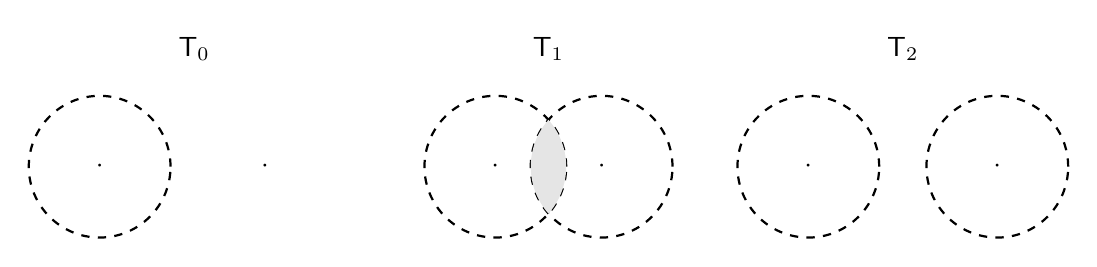
\begin{tikzpicture}[scale = 0.3]
		\draw[black,thick,dashed] (4,0) circle (3); 
		\node at (4,0) {$\cdot$};
		\node at (8,5) {$\mathsf{T}_0$};
		\node at (11,0) {$\cdot$};
		
		\draw[black,thick,dashed] (20.75,0) circle (3);
		\node at (20.75,0) {$\cdot$};
		\node at (23, 5) {$\mathsf{T}_1$};
		\draw[black,thick,dashed] (25.25,0) circle (3);
		\node at (25.25,0) {$\cdot$};
		
		\begin{scope}
			\clip (20.75,0) circle (3);
			\fill[black!10] (25.25,0) circle (3);
		\end{scope}
		
		\draw[black,thick,dashed] (34,0) circle (3);
		\node at (34,0) {$\cdot$};
		\node at (38,5) {$\mathsf{T}_2$};
		\draw[black,thick,dashed] (42,0) circle (3);
		\node at (42,0) {$\cdot$};
	\end{tikzpicture}
\end{center}

\begin{mathSection}
	\begin{defn}
		A topology for $X$ is \textbf{Kolmogorov} (or $\mathsf{T}_0$) if for every two elements $x_1, x_2 \in X$ there exists a verifiable set $U \in \mathsf{T}_X$ containing one element but not the other. That is: either $x_1 \in U$ while $x_2 \notin U$ or $x_1 \notin U$ while $x_2 \in U$.
	\end{defn}
	\begin{defn}
	A topology for $X$ is \textbf{Fr\'echet} (or $\mathsf{T}_1$) if for every two elements $x_1, x_2 \in X$ there exist two, not necessarily disjoint, verifiable sets $U_1, U_2 \in \mathsf{T}_X$ each containing only one element. That is: $x_1 
	\in U_1$ and $x_2 \in U_2$.
\end{defn}
	\begin{defn}
	A topology for $X$ is \textbf{Hausdorff} (or $\mathsf{T}_2$) if for every two elements $x_1, x_2 \in X$ there exist two disjoint verifiable sets $U_1, U_2 \in \mathsf{T}_X$ each containing one element. That is: $U_1 \cap U_2 = \emptyset$, $x_1 
	\in U_1$ and $x_2 \in U_2$.
\end{defn}
\begin{remark}
	Note that $\mathsf{T}_2$ implies $\mathsf{T}_1$ which in turn implies $\mathsf{T}_0$.
\end{remark}

\end{mathSection}

How do these properties relate to experimental domains? Consider two possibilities for a domain, for example \statement{that is a cat} and \statement{that is a swan}. We can always find a verifiable statement, such as \statement{that animal has feathers}, that we can use to distinguish one possibility from the other. This means that, given two different possibilities, we can always find a verifiable set that contains one and not the other: the natural topology for any set of possibilities is always $\mathsf{T}_0$.

Now suppose two possibilities are approximately verifiable as we defined in Definition \ref{def_approximately_verifiable}. For example, \statement{the mass of the photon is exactly 0 eV} or \statement{the mass of the photon is exactly $10^{-20}$ eV}. We can find two verifiable statements \statement{the mass of the photon is less than $10^{-25}$ eV} and \statement{the mass of the photon is more than $10^{-25}$ eV} each compatible with only one possibility. This means that, given two approximately verifiable possibilities, we can find two verifiable sets each containing only one possibility: if all possibilities are approximately verifiable then the natural topology is $\mathsf{T}_1$.

Now suppose two possibilities are experimentally distinguishable as we defined in Definition \ref{1_def_experimentally_distinguishable}. Then, by \ref{1_prop_experimentally_distinguishable_is_disjoint_approximations}, we can find two disjoint approximations. In the example before, the two verifiable statements were in fact incompatible. This means that, given two approximately verifiable possibilities, we can find two disjoint verifiable sets each containing only one possibility: if all possibilities are experimentally distinguishable then the natural topology is $\mathsf{T}_2$.

\begin{mathSection}
	\begin{prop}
	The natural topology of a set of possibilities is Kolmogorov (or $\mathsf{T}_0$).
\end{prop}
\begin{proof}
	Let $X$ be the set of possibilities for an experimental domain $\edomain$. Let $x_1, x_2 \in X$ be two distinct possibilities. Each of them can be expressed as a minterm of a basis $\basis \subseteq \edomain$. Since the two possibilities are distinct, there must exist a verifiable statement $\stmt[e] \in \basis$ that appears negated in one conjunction but not the other. That is, $\stmt[e]$ is compatible with only one possibility. Since the verifiable set associated with a verifiable statement contains only the possibilities compatible with said statement, the verifiable set of $\stmt[e]$ either contains $x_1$ or $x_2$ but not both. The topology is therefore Kolmogorov (or $\mathsf{T}_0$).
\end{proof}
\begin{prop}
	The natural topology of a set of possibilities is Fr\'echet (or $\mathsf{T}_1$) if and only if all possibilities are approximately verifiable.
\end{prop}
\begin{proof}
	% TODO: Could be shorten since it is sufficient to just prove one side (I.e. given x,y in X, find U containing x but not y. No need to find another set for y. Because the points were arbitrary there is no loss of generality).
	Suppose all possibilities in $X$ for an experimental domain $\edomain_X$ are approximately verifiable. Let $x_1, x_2 \in X$ be two possibilities, then we can find two sequences of verifiable statements $\{\stmt_i^1\}_{i=1}^\infty, \{\stmt_j^2\}_{j=1}^\infty \in \edomain_X$ such that $x_1=\bigAND\limits_{i=1}^\infty \stmt_i^1$ and $x_2=\bigAND\limits_{j=1}^\infty \stmt_j^2$. We can assume the sequences are monotone with respect to narrowness, that is $\stmt_{i+1}^1 \narrower \stmt_i^1$, as we can always create a monotone sequence from one that is not by taking the sequence of finite conjunction, that is $\hat{\stmt}_k^1=\bigAND\limits_{i=1}^k \stmt_i^1$. If $x_1 \neq x_2$, then $x_1 \AND x_2 \equiv \impossibility$ since different possibilities are incompatible. Therefore we must have $x_1 \AND \stmt_j^2 \equiv \impossibility$ and $\stmt_i^1 \AND x_2 \equiv \impossibility$ from some $i,j \geq 1$ or the limits would not be incompatible. In terms of verifiable sets we have $x_2 \notin U(\stmt_i^1)$ and $x_1 \notin U(\stmt_j^2)$. For any two distinct possibilities we can find two verifiable sets each containing one: the natural topology is $\mathsf{T}_1$.

	Conversely, suppose the natural topology $\mathsf{T}_X$ for the possibilities $X$ for an experimental domain $\edomain_X$ is $\mathsf{T}_1$. Let $x \in X$ be a possibility. Consider the collection, not necessarily countable, of all verifiable sets $\{U_i\}_{i \in I} \subset \mathsf{T}_X$ such that they contain $x$. Consider their intersection $U_x = \bigcap\limits_{i \in I} U_i$. It will contain $x$ since all $U_i$ contain $x$. It will not contain anything else: since the topology is $\mathsf{T}_1$, for every other possibility $\hat{x}$ there is always an open set $U_i$ that does not contain it. Therefore $U_x = \{x\}$. Because the natural topology is second countable, we can find a countable basis $\basis$ and rewrite the arbitrary intersection into $\{x\} = \bigcap\limits_{i=1}^\infty V_i$ a countable intersection of elements $V_i \in \basis$ of the basis. Let $\{\stmt_i\}_{i=1}^\infty$ be the sequence of verifiable statements such that $U(\stmt_i) = V_i$ for every $i$. Then $x=\bigAND\limits_{i=1}^\infty \stmt_i$ which means $x$ is approximately verifiable.

\end{proof}
\begin{prop}
	The natural topology of a set of possibilities is Hausdorff (or $\mathsf{T}_2$) if and only if all possibilities are pairwise experimentally distinguishable.
\end{prop}
\begin{proof}
	Suppose all possibilities in $X$ for an experimental domain $\edomain_X$ are pairwise experimentally distinguishable. Then, by \ref{1_prop_experimentally_distinguishable_is_disjoint_approximations}, given two possibilities $x_1, x_2 \in X$ we can find two verifiable statements $\stmt_1, \stmt_2 \in \edomain_X$ such that $\stmt_1 \ncomp \stmt_2$, $x_1 \narrower \stmt_1$ and $x_2 \narrower \stmt_2$. In terms of verifiable sets we have $U(\stmt_1) \cap U(\stmt_2) = \emptyset$, $x_1 \in U(\stmt_1)$ and $x_2 \in U(\stmt_2)$. The topology is $\mathsf{T}_2$.
	
	Conversely, suppose the natural topology $\mathsf{T}_X$ for the possibilities $X$ for an experimental domain $\edomain_X$ is $\mathsf{T}_2$. Given two possibilities $x_1, x_2 \in X$ we can find two verifiable sets $U_1, U_2 \in \mathsf{T}_X$ such that $U_1 \cap U_2 = \emptyset$, $x_1 \in U_1$ and $x_2 \in U_2$. Since $U_1, U_2 \in \mathsf{T}_X$, we can find two corresponding verifiable statements $\stmt_1, \stmt_2 \in \edomain_X$ such that $U(\stmt_1) = U_1$ and $U(\stmt_2) = U_2$. We have $\stmt_1 \ncomp \stmt_2$, $x_1 \narrower \stmt_1$ and $x_2 \narrower \stmt_2$ and by \ref{1_prop_experimentally_distinguishable_is_disjoint_approximations} the possibilities are pairwise experimentally distinguishable.
\end{proof}
\end{mathSection}

\section{Sigma-algebras}

In the same way that experimental domains find a natural mathematical representation as topological spaces, theoretical domains find a natural mathematical representation in $\sigma$-algebras. The main result of this section is that a theoretical domain provides a natural $\sigma$-algebra on its possibilities.

Like topologies, $\sigma$-algebras are fundamental in mathematics as they allow us to construct measures (i.e.~assigning sizes to sets), limits for sequences of sets and probability spaces. It is again fitting that theoretical domains are associated to such a fundamental mathematical structure.

Let's first review what a $\sigma$-algebra is. The general idea is that we have a set $X$ of elements which we call points, and we have a collection of subsets of $X$ such that it is closed under complement and countable union, contains the empty set and contains the whole set $X$. For example, suppose $X = \{1,2,3\}$ then  $\{\{\},\{1\},\{1,2,3\}\}$ is not a $\sigma$-algebra while $\{\{\},\{1\}, \{2,3\},\{1,2,3\}\}$ is. The first one is missing the complement of $\{1\}$.

\begin{mathSection}
	\begin{defn}
		Let $X$ be a set. A \textbf{$\sigma$-algebra} on $X$ is a collection $\Sigma_X$ of subsets of $X$ closed under complement and countable union such that it contains $X$.
	\end{defn}
\end{mathSection}

Note that $\sigma$-algebras are also closed under countable intersections, since these can be expressed in terms of complements and countable unions.

In the previous section we saw how each verifiable statement can be expressed as the conjunction of a set of possibilities, how the operations on statements can be expressed as operations on the verifiable sets and how all the verifiable sets form a topology. The same is true for theoretical statements, with the only difference being that we will end up with a collection of sets that is closed under complement and countable union since the theoretical domain is closed under negation and countable disjunction.

\begin{mathSection}
	
	\begin{defn}
		Let $\tdomain$ be a theoretical domain and $X$ its possibilities. We define the map $A : \tdomain \rightarrow 2^X$ that for each theoretical statement $\stmt \in \tdomain$ returns the set of possibilities compatible with it. That is, $A(\stmt)\equiv\{ x \in X \, | \, x \comp \stmt\}$. We call $A(\stmt)$ the \textbf{theoretical set} of possibilities associated with $\stmt$
	\end{defn}
	
	\begin{prop}
		Let $X$ be the set of possibilities for a theoretical domain $\tdomain$. $X$ has a natural $\sigma$-algebra given by the collection of all theoretical sets $\Sigma_X=A(\tdomain)$.
	\end{prop}
	
	\begin{proof}
	The theoretical sets for the certainty and the impossibility correspond to the full set and empty set respectively. Formally, $A(\certainty) = \{ x \in X \, | \, x \comp \certainty\} = X$ while $A(\impossibility) = \{ x \in X \, | \, x \comp \impossibility\} = \emptyset$. Therefore $X, \emptyset \in A(\tdomain)$ since $\certainty, \impossibility \in \tdomain$.

	The complement of a theoretical set corresponds to the theoretical set of the negation and therefore it is a theoretical set. Formally, $A(\stmt)^C = \{ x \in X \, | \, x \ncomp \stmt\} =  \{ x \in X \, | \, x \comp \NOT\stmt\} = A(\NOT\stmt)$.

	The countable union of verifiable sets corresponds to the verifiable set of the countable disjunction and therefore it is a theoretical set. Formally, $A(\stmt_1\OR\stmt_2) = \{ x \in X \, | \, x \comp \stmt_1\OR\stmt_2\} =  \{ x \in X \, | \, x \comp \stmt_1 \, or \, x \comp \stmt_2\} = \{ x \in X \, | \, x \comp \stmt_1\} \cup \{ x \in X \, | \, x \comp \stmt_2\} = A(\stmt_1) \cup A(\stmt_2)$. This generalizes to countable disjunctions.

	The collection $\Sigma_X=A(\tdomain)$ is therefore a $\sigma$-algebra by definition since it satisfies all its properties.
	\end{proof}
\end{mathSection}

There is also a special link between topologies and $\sigma$-algebras. As one may want to construct measures and probability spaces on topological spaces, there is a standard way to construct a $\sigma$-algebra from a topology. This object, called Borel algebra, is the smallest $\sigma$-algebra that contains all verifiable sets defined by the topology. The $\sigma$-algebra defined by a theoretical domain is none other than the Borel algebra of the topology defined by the corresponding experimental domain.

\begin{mathSection}
	
	\begin{defn}
		Let $(X, \mathsf{T})$ be a topological space. Its \textbf{Borel algebra} is the collection $\Sigma_X$ of subsets of $X$ generated by countable union, countable intersection and complement from the verifiable sets.
	\end{defn}
	
	\begin{prop}
		The natural $\sigma$-algebra for a set of possibilities is the Borel algebra of its natural topology.
	\end{prop}
	
	\begin{proof}
		Since the theoretical domain can be generated by a basis of the experimental domain, the natural $\sigma$-algebra can be generated by a sub-basis of the natural topology. This means that it is also generated by countable union, countable intersection and negation from the verifiable sets of the natural topology.
	\end{proof}
\end{mathSection}

This fundamental link between experimental domains and topology on one side and theoretical domains and $\sigma$-algebra on the other is important for multiple reasons.

From a practical standpoint, it guarantees that these mathematical tools can always be used in science. Since experimental and theoretical domains are general constructs, any branch of scientific investigation can use techniques and results from topology and $\sigma$-algebras for calculations or for characterizing the domain at hand.

From a conceptual standpoint it provides a Rosetta stone, i.e a way to translate, between the mathematical concepts and the scientific ones. It gives a precise scientific meaning to the mathematical tools and everything built on top of them. Every single step in a calculation, every single argument in a proof can be given a clear, and possibly insightful, physical meaning. It grounds the abstract mathematical language in more concrete scientific objects. This in turn helps clarify the science described by common mathematical tools, unearthing possible hidden assumptions or simplifications about the physical systems being studied.

This connection explains why these mathematical tools have found such successful application in the physical sciences.

\section{Decidable domains}

We conclude this chapter by analyzing decidable domains, those for which we can experimentally test both the truth and the falsehood of all statements. For example, the domain for animal identification and the domain for the amount of money in my pocket can be considered decidable as we can typically tell experimentally whether \statement{this animal has whiskers} or not, or whether \statement{there is more than one dollar and fifty cents in my pocket} or not.

Decidable domains have special characteristics and are easier to study. Since we can verify the negation, any theoretical statement is also verifiable. And since all theoretical statements are verifiable, so are the possibilities. That is, we can verify that \statement{this animal is a cat} and that \statement{there are two dollars and thirty cents in my pocket}. As all statements can be expressed as a disjunction of possibilities, the possibilities themselves form a countable basis. For example, \statement{there is more than one dollars and fifty cents in my pocket} can be expressed as the disjunction of the appropriate statements of the form \statement{there are x dollars and y cents in my pocket}.

\begin{mathSection}
\begin{defn}
	An experimental domain $\edomain_X$ is \textbf{decidable} if all statements in the domain are decidable. Formally, for every $\stmt \in \edomain_X$ we have $\NOT\stmt \in \edomain_X$.
\end{defn}

\begin{prop}\label{1_prop_decidable_domain_properties}
	Let $\edomain_X$ be an experimental domain. The following are equivalent:
	\begin{enumerate}
		\item the experimental domain is decidable
		\item the experimental domain and its theoretical domain coincide
		\item all possibilities are verifiable
		\item the possibilities form a countable basis.
	\end{enumerate}
\end{prop}

\begin{proof}
	To prove 2 from 1, suppose $\edomain_X$ is a decidable experimental domain. As $\edomain_X$ is decidable, it is already closed under negation and therefore all statements in its theoretical domain $\tdomain_X$ are already in $\edomain_X$.
	
	To prove 3 from 2, suppose $\edomain_X$ coincides with its theoretical domain $\tdomain_X$. As each possibility is a theoretical statement, it is also a verifiable statement.
	
	To prove 4 from 3, suppose the possibilities are verifiable. Note that the possibilities can generate all other statements through disjunction. To show $X$ is countable, consider a countable basis $\basis \subseteq \edomain_X$. Because the possibilities are verifiable statements, they can be generated from $\basis$ by finite conjunction and countable disjunction. Moreover, since the possibilities are the narrowest statements that are not impossible, they can be generated from $\basis$ using finite conjunction only. Since $\basis$ is countable and $X$ is generated by $\basis$ through finite conjunction, $X$ can be at most countable. Therefore $X$ is a countable basis.
	
	To prove 1 from 4, suppose the possibilities $X$ form a countable basis. Then each possibility is verifiable and so is their countable union. The negation of a verifiable statement can be expressed as the countable union of possibilities, and is therefore verifiable. All statements in the experimental domain are decidable and therefore the domain is decidable.
\end{proof}
\end{mathSection}

As the possibilities for a decidable domain must form a countable basis, their cardinality can't be greater than countable. That is: only domains that are non-decidable can have possibilities with cardinality of the continuum. In this sense they are more constrained and simpler to study.

Mathematically, the natural topology corresponds to the discrete topology: the one for which any subsets of the possibilities is a verifiable set. That is, the topology is simply the set of all possible sets of possibilities. The cardinality of the possibility is therefore enough to determine the topology of the space, which means that one number is enough to characterize the space.

\begin{mathSection}
\begin{defn}
	A topology $\mathsf{T}_X$ on a set $X$ is called \textbf{discrete} if it contains every subset of $X$.
\end{defn}

\begin{thrm}[Decidability is discreteness]\label{thrm_decidablity_is_discreteness}
	The natural topology of the possibilities $X$ for a domain $\edomain_X$ is discrete if and only if the domain is decidable.
\end{thrm}
\begin{proof}
	Suppose $\edomain_X$ is decidable. Let $U \subseteq X$ be a subset of possibilities. The statement $\stmt = \bigOR\limits_{x \in U} x$ is generated from $X$ through countable disjunction. Since $\edomain_X$ is decidable, $X$ is a countable basis and $\stmt$ is verifiable. Therefore $U$ is a verifiable set and it is contained in the natural topology. The natural topology of $X$ is discrete by definition.
	
	Now suppose $\edomain_X$ is such that the natural topology for its possibilities $X$ is discrete. Let $\stmt = \bigOR\limits_{x \in U} x$ be a statement. Since the topology is discrete, $U$ is part of the topology and $\stmt$ is verifiable. Consider its negation $\NOT\stmt = \bigOR\limits_{x \in U^C} x$. Since the topology is discrete, $U^C$ is also part of the topology and $\NOT\stmt$ is verifiable. This means $\stmt$ is decidable. Since every statement in $\edomain_X$ is decidable, the domain is decidable.
\end{proof}
	
\end{mathSection}

Note, though, that discrete does not imply finite or vice-versa. The domain for extra-terrestrial life is finite but is not decidable as we cannot verify that \statement{there is no extra-terrestrial life}. The domain for the amount of money in my pocket, instead, is decidable but not necessarily finite as I could potentially have an arbitrarily large amount.

\section{Summary}

In this first chapter we have laid down the foundations for our general mathematical theory of experimental science. We have seen how it is grounded in the logic of verifiable statements, which is more limited than the logic of pure statements as it has to deal with the practical constraints introduced by the termination of the tests.


\begin{center}
	\begin{tikzpicture}
		\node[draw, minimum width=10.5cm, minimum height=5.3cm, rounded corners=5mm] (bdx) {};
		\node[align=center, below] at ([yshift=-1mm]bdx.north) {\textbf{Theoretical statements} \\statements associated with an experimental test};
		\node[align=center, above left] at (bdx.157) {$\tdomain_X$};
		\node[align=center, above] at (bdx.north) {\textbf{Statements} ($\AND$ $\OR$ $\NOT$ $\impossibility$ $\certainty$)};
		
		\node[ellipse, draw, minimum width=5cm, minimum height=3.5cm, align=center, inner xsep=-2mm] (vs) at ([xshift=-1.85cm, yshift=-5mm]bdx) {\textbf{Verifiable statements}\\[1mm]
			if true, test always\\
			succeeds};
		\node[align=center, above left] at (vs.145) {$\edomain_X$};
		\node[ellipse, draw, minimum width=4.2cm, minimum height=2.7cm, align=center,inner xsep=0mm] (poss) at ([xshift=2.25cm,yshift=-7mm]bdx) {\textbf{Possibilities}\\[1mm]
			experimentally\\
			distinguishable\\
			cases
		};
		\node[align=center, above right] at (poss.90-55) {$X$};
		
		\node[draw, minimum width=4.8cm, minimum height=3cm, rounded corners=5mm, anchor=north west] (sx) at ([yshift=-5mm]bdx.south west) {};
		\node[align=center, above] at ([xshift=-3mm,yshift=0.5mm]sx.-115) {\textbf{Borel sets}};
		\node[align=center, above left] at (sx.155) {$\Sigma_X$};
		
		\node[ellipse, minimum width=3cm, minimum height=2cm, draw] (os) at ([xshift=3mm,yshift=1mm]sx) {\textbf{Open sets}};
		\node[align=center, above left] at (os.150) {$\mathsf{T}_X$};
		\node[ellipse, minimum width=2.8cm, minimum height=1.8cm, draw] (point) at([yshift=-1mm]os-|poss)  {\textbf{Points}};
		\node[align=center, below=3.6cm] at (bdx.south) {\textbf{Sets} ($\cup$ $\cap$ $\complement$ $X$ $\emptyset$)};
		\node[align=center, above right] at (point.90-55) {$X$};
		
		\coordinate (z) at (bdx.south);
		\draw[stealth'-stealth'] (sx.130)--(z-|sx.130);
		\draw[stealth'-stealth'] (vs.south) to (os.90);
		\draw[stealth'-stealth'] (poss.south) to (point);
		\draw[stealth'-stealth'] ([xshift=2mm]sx.east)--+(8mm,0);
		
		\draw[gray, dashed, thick] (-6,-2.75)--+(11.5,0);
	\end{tikzpicture}
\end{center}


We saw that we can group verifiable statements into experimental domains which must have a countable basis to allow us to test any statement within an indefinite amount of time. We saw how to construct theoretical domains to find all the theoretical statements that can be associated to an experimental test. And we saw how the possibilities are those statements that, if true, give a complete prediction for all statements in the domain.

We have seen that, because of the disjunctive normal form, each verifiable and theoretical statement is equivalent to a set of possibilities and how logic operations and relationships become set operations and relationships. As such, the experimental and theoretical domains respectively provide a natural topology and $\sigma$-algebra for the possibilities.

What we have ended up with is a conceptual framework that captures the necessary elements of scientific practice and codifies them into a symbolic representation with a well defined meaning. There is no guesswork as to what the points of our spaces are: they are the possibilities, statements that provide a complete description for the domain. We do not have to provide an ``interpretation" as to what the sets of a topology represent: they correspond to verifiable statements. All the objects have a clear definition and meaning from the start, we know which ones are necessary and to what extent they are physical or idealized. This will provide a much more solid foundation to the rest of the work, which will ultimately allow us to understand much better the fundamental physical theories and the connections between them and to other areas of scientific thought.



\newpage

\section{Reference sheet}

\begin{tabular}{p{0.2\textwidth} p{0.3\textwidth} p{0.5\textwidth}}
	& Name & Meaning  \\ 
	\hline 
	$\Bool$  & Boolean domain & the set of possible truth values \\ 
	&  & i.e.~$\Bool = \{\TRUE, \FALSE\}$ \\ 
	\hline 
	$\logCtx$ & logical context & a set of statements with well defined logical relationships \\ 
	\hline 
	$\stmt \in \logCtx$ & statement & an assertion with a well defined truth value \\ 
	\hline 
	$\truth : \logCtx \to \Bool$ & the truth function & returns whether a statement is true or not  \\ 
	\hline 
	$\pAss \subseteq \Bool^\logCtx$& possible assignments & the logically consistent truth value combinations that can be assigned to the statements \\ 
	\hline 
	$\certainty$ & certainty & a statement that can only be true (i.e.~it is true in all possible assignments) \\ 
	\hline 
	$\impossibility$ & impossibility & a statement that can never be true (i.e.~it is false in all possible assignments) \\ 
	\hline 
	& contingent statement & a statement that can be either true or false depending on the possible assignment \\ 
	\hline 
	$\NOT \stmt$ & negation (logical NOT) & the statement whose truth value is always opposite \\ 
	\hline 
	$\stmt_1 \AND \stmt_2$ & conjunction (logical AND) & the statement that is true only if all statements are true \\ 
	\hline 
	$\stmt_1 \OR \stmt_2$ & disjunction (logical OR) & the statement that is true if any of the statements is true \\ 
	\hline 
	$\stmt_1 \equiv \stmt_2$ & equivalence & whether each statement is a logical consequence of the other (i.e.~they must have the same value in every possible assignment) \\ 
	\hline 
	$\stmt_1 \narrower \stmt_2$ & narrower than & whether the first statement is more specific than the second (i.e.~in every possible assignment, if the first is true than the second must be also true) \\ 
	\hline 
	$\stmt_1 \broader \stmt_2$ & broader than & whether the second statement is narrower than the first \\ 
	\hline 
	$\stmt_1 \comp \stmt_2$ & compatibility & whether both statement can be true at the same time (i.e.~there is a possible assignment in which they are both true) \\
	\hline 
	$\stmt_1 \indep \stmt_2$ & independence & whether both statement can be true at the same time (i.e.~there is a possible assignment for each combination of their possible truths) \\
	\hline 
	& minterm & a conjunction where each statement appears once, either negated or not \\
	\hline 
	$\stmt \in \vstmtSet$ & verifiable statement & a statement that can be validated experimentally\\ 
	\hline 
	$\edomain$ & experimental domain & a set of verifiable statements that can be tested in an indefinite amount of time (i.e.~a set of statements closed under finite conjunction and countable disjunction, that precisely contains the certainty, the impossibility and a set of verifiable statements generated by a countable basis) \\ 
	\hline 
	$\basis \in \edomain$ & basis & a set of verifiable statements from which all others can be constructed\\ 
			
\end{tabular} 

\newpage

\begin{tabular}{p{0.2\textwidth} p{0.3\textwidth} p{0.5\textwidth}}
	& Name & Meaning  \\ 
	\hline 
	$\tdomain$ & theoretical domain & the set of all statements constructed from an experimental domain that can be associated with an experimental test\\ 
	\hline 
	& approximately verifiable & when a statement is not verifiable but is the limit of a sequence of statements that are\\ 
	\hline 
	$X$ & possibilities of a domain & those statements that, if true, determine the value of all verifiable statements of a domain\\ 
	\hline 
	$\estPoss$ & established possibility & a possibility for which at least a verifiable statement is true (i.e.~it can be established experimentally)\\ 
	\hline 
	$\resPoss$ & residual possibility & if it exists, the possibility for which all verifiable statements are false (i.e.~the remaining case that cannot be established experimentally)\\ 
	
\end{tabular} 


\chapter{Domain combination and relationships}

We continue our investigation of the fundamental mathematical structures for experimental science by studying what happens when we have more than one experimental domain. We will define \textbf{experimental relationships} between experimental domains, which capture either causal or inference relationships between them. We will see that these correspond to continuous functions in the natural topology.

We will take two or more domains and merge all the experimental information that can be gathered through them into a \textbf{combined domain}. We will study how the set of possibilities of the combined domain depends not only on the original domains, but also on the relationships between them. These will also determine the natural topology that can vary from the product topology all the way to the disjoint union topology.

We will also show that experimental relationships, under suitable conditions, can themselves be verified experimentally by constructing the \textbf{relationship domain} for which its possibilities correspond to the possible relationships.

\section{Dependence and equivalence between domains}

The first thing we want to be able to characterize, when dealing with more than one domain, is when there exists a relationship between them. For example, consider the domains for the temperature and height of a mercury column or the domains for the temperature and density of water. How do we express, in this framework, the fact that these domains are connected?

We have two ways to define these relationships between domains. The first is in terms of inference: any measurement on the height of a mercury column is an indirect measurement on its temperature; any experimental test on the density of water is an indirect experimental test on its temperature. The second is in terms of causes: the height of the mercury column depends on its temperature; the density of water is a function of its temperature. The main result of this section is to show that these definitions are equivalent and that the dependent domain can be seen as a sub-domain of the other.

Suppose $\edomain_X$ represents the domain for the temperature of a mercury column while $\edomain_Y$ represents the domain for its height. Since we know that an increase in temperature makes the metal expand, we can infer the temperature of the mercury column by looking at its height. For example, if we verify that \statement{the height of the mercury column is between 24 and 25 millimeters} we will be able to infer that \statement{the temperature is between 24 and 25 Celsius}. That is, given a verifiable statement $\stmt_Y$ we have another verifiable statement $\stmt_X$ that is going to be true if and only if the first one is, that is $\stmt_Y\equiv\stmt_X$.

Note that the inference is between verifiable statements and not intervals. For example, the verifiable statement \statement{the water density is between 999.8 and 999.9 kg/$m^3$} will correspond to \statement{the water temperature is between 0 and 0.52 Celsius}$\OR$\statement{the water temperature is between 7.6 and 9.12 Celsius} as water is most dense at 4 Celsius. The disjunction of verifiable statements is still a verifiable statement so we are still inferring one verifiable statement from the other. For each verifiable statement in $\edomain_Y$ we can find a verifiable statement in $\edomain_X$ that is verified if and only if the first is. That is: an inference relationship is a map from $\edomain_Y$ to $\edomain_X$ that preserves equivalence.

\begin{mathSection}
	\begin{defn}
		An \textbf{inference relationship} between two experimental domains establishes that testing a verifiable statement in one means testing a verifiable statement in the other. Formally, an inference relationship between two experimental domains $\edomain_X$ and $\edomain_Y$ is a map $\erel: \edomain_Y \to \edomain_X$ such that $\erel(\stmt_Y) \equiv \stmt_Y$. In other words: it is an equivalence-preserving map between experimental domains.
	\end{defn}
\end{mathSection}

An inference relationship is essentially an injection that preserves equivalence instead of identity. In terms of equality, the two statements \statement{the height of the mercury column is between 24 and 25 millimeters} and \statement{the temperature is between 24 and 25 Celsius} are different, but they are the same in terms of equivalence. In this sense, the dependent domain is already contained within the other domain. This means we can define domain inclusion and equivalence based on inference relationships.

\begin{mathSection}
	\begin{defn}
		An experimental domain $\edomain_Y$ is \textbf{dependent} on another experimental domain $\edomain_X$, noted $\edomain_Y \subseteq \edomain_X$, if there exists an inference relationship $\erel: \edomain_Y \to \edomain_X$.
	\end{defn}
	\begin{coro}\label{prop_domain_subset_is_dependence}
		Let $\edomain_X$ be an experimental domain. Let $\edomain_Y$ be a subset of statements of $\edomain_X$ that form an experimental domain (i.e. contains impossibility, certainty and is closed under finite conjunction and countable disjunction). Then $\edomain_Y \subseteq \edomain_X$.
	\end{coro}
	\begin{proof}
		Let $\iota : \edomain_Y \to \edomain_X$ be the inclusion map. This is an inference relationship since $\iota(\stmt_Y) = \stmt_Y \equiv \stmt_Y$ therefore $\edomain_Y$ depends on $\edomain_X$.
	\end{proof}
	\begin{defn}
		Two experimental domains $\edomain_X$ and $\edomain_Y$ are \textbf{equivalent} $\edomain_X \equiv \edomain_Y$ if $\edomain_X$ depends on $\edomain_Y$ and vice-versa.
	\end{defn}
	\begin{coro}
		Domain equivalence satisfies the following properties:
		\begin{itemize}
			\item reflexivity: $\edomain \equiv \edomain$
			\item symmetry: if $\edomain_X \equiv \edomain_Y$ then $\edomain_Y \equiv \edomain_X$
			\item transitivity: if $\edomain_X \equiv \edomain_Y$ and $\edomain_Y \equiv \edomain_Z$ then $\edomain_X \equiv \edomain_Z$
		\end{itemize}
		and is therefore an \textbf{equivalence relationship}.
	\end{coro}
	\begin{proof}
		For reflexivity, $\edomain$ is a subset of $\edomain$ that is an experimental domain, therefore $\edomain \subseteq \edomain$ by \ref{prop_domain_subset_is_dependence}. Equivalence follows by symmetry.
		
		For symmetry, suppose $\edomain_X \equiv \edomain_Y$, then $\edomain_Y \subseteq \edomain_X$ and $\edomain_X \subseteq \edomain_Y$ and therefore $\edomain_Y \equiv \edomain_X$.
		
		For transitivity, suppose $\edomain_X \equiv \edomain_Y$ and $\edomain_Y \equiv \edomain_Z$. Then we have the following inference relationships: $\erel_{XY} : \edomain_X \to \edomain_Y$, $\erel_{YX} : \edomain_Y \to \edomain_X$, $\erel_{YZ} : \edomain_Y \to \edomain_Z$, $\erel_{ZY} : \edomain_Z \to \edomain_Y$. We can define the function compositions $\erel_{XZ} = \erel_{YZ} \circ \erel_{XY}$ and $\erel_{ZX} = \erel_{YX} \circ \erel_{ZY}$. These are inference relationships since $\stmt_X \equiv \erel_{XY}(\stmt_X) \equiv \erel_{YZ}(\erel_{XY}(\stmt_X))$ and $\stmt_Z \equiv \erel_{ZY}(\stmt_Z) \equiv \erel_{YX}(\erel_{ZY}(\stmt_Z))$. Therefore $\edomain_X \equiv \edomain_Z$.
	\end{proof}
\end{mathSection}


\begin{center}
	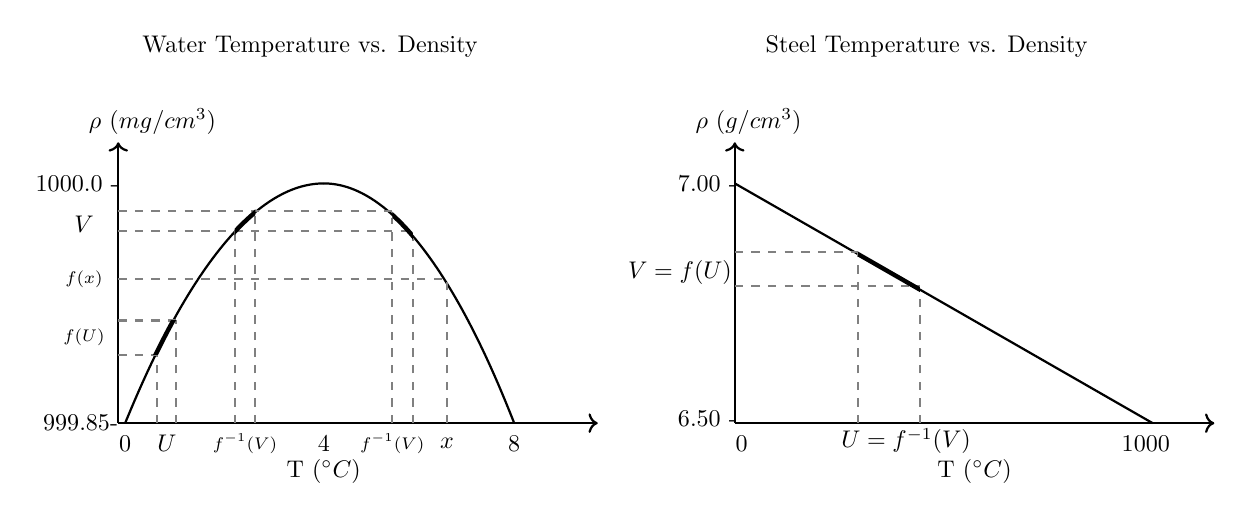
\begin{tikzpicture}[thick,scale=0.87, every node/.style={scale=0.87}]
		
		\draw[thick,->] (-1,3) -- (6,3);
		\draw[thick,->] (-1,3) -- (-1,7.1);
		
		\node at (-0.5,7.4) {$\rho$ ($mg/cm^3$)};
		\node at (2,2.3) {T ($^\circ C$)};
		
		\node at (2,2.7) {4};
		\node at (4.78,2.7) {8};
		\node at (-0.9,2.7) {0};
		
		\node at (-1.6,6.5) {1000.0 -};
		\node at (-1.55,3.01) {999.85-};
		
		
		\draw (2,6.5) parabola (4.78,3);
		\draw (2,6.5) parabola (-0.9,3);
		
		\draw[gray,thick,dashed] (-1,5.1) -- (3.8,5.1);
		
		\draw[gray,thick,dashed] (3.8,3) -- (3.8,5.1);
		
		\node at (3.8,2.7) {$x$};
		\node at (-1.5,5.1) {$\scriptstyle f(x)$};
		
		
		\draw[gray,thick,dashed] (-1,4.5) -- (-0.16,4.5);
		\draw[gray,thick,dashed] (-1,4) -- (-0.43,4);
		
		\draw[gray,thick,dashed] (-0.16,3) -- (-0.16,4.5);
		\draw[gray,thick,dashed] (-0.43,3) -- (-0.43,4);
		
		\node at (-0.29,2.7) {$U$};
		\node at (-1.5,4.25) {$\scriptstyle f(U)$};

		
		\draw[gray,thick,dashed] (0.7,3) -- (0.7,5.8);
		\draw[gray,thick,dashed] (1,3) -- (1,6.1);
		
		\draw[gray,thick,dashed] (-1,5.8) -- (3.25,5.8);
		\draw[gray,thick,dashed] (-1,6.1) -- (3,6.1);
		
		\draw[gray,thick,dashed] (3,3) -- (3,6);
		\draw[gray,thick,dashed] (3.3,3) -- (3.3,5.7);
		
		\node at (0.85,2.7) {$\scriptstyle f^{-1}(V)$};
		\node at (3.0,2.7) {$\scriptstyle f^{-1}(V)$};
		\node at (-1.5,5.9) {$V$};
		
		\begin{scope}
			\clip (-0.5,4) rectangle (0.2,4.5);
			\draw[black, ultra thick] (2,6.5) parabola (-0.9,3);
		\end{scope}
		
		\begin{scope}
			\clip (0.7,5.2) rectangle (1,6.5);
			\draw[black, ultra thick] (2,6.5) parabola (-0.9,3);
		\end{scope}
		
		\begin{scope}
			\clip (3,5) rectangle (3.3,6.3);
			\draw[black, ultra thick] (2,6.5) parabola (4.78,3);
		\end{scope}
		
		
		\draw[thick,->] (8,3) -- (15,3);
		\draw[thick,->] (8,3) -- (8,7.1);
		
		\node at (11.5,2.3) {T ($^\circ C$)};
		\node at (8.2,7.4) {$\rho$ ($g/cm^3$)};
		
		\draw (8,6.5) -- (14.1,3);
		
		\node at (7.6,6.5) {7.00 -};
		\node at (7.6,3.06) {6.50 -};
		\node at (14,2.7) {1000};
		\node at (8.1,2.7) {0};
		
		\draw[gray,thick,dashed] (8,5.5) -- (9.8,5.5);
		\draw[gray,thick,dashed] (8,5) -- (10.7,5);
		
		\draw[gray,thick,dashed] (9.8,3) -- (9.8,5.5);
		\draw[gray,thick,dashed] (10.7,3) -- (10.7,4.9);
		
		\begin{scope}
			\clip (9.8,4.5) rectangle (10.7,5.5);
			\draw[black, ultra thick] (8,6.5) -- (14.1,3) ;
		\end{scope}
		
		
		\node at (10.5,2.74) {$U=f^{-1}(V)$};
		\node at (7.2,5.2) {$V=f(U)$};
		
		
		\node at (1.8,8.5) {Water Temperature vs. Density};
		\node at (10.8,8.5) {Steel Temperature vs. Density};
	\end{tikzpicture}
\end{center}


It should be evident that we cannot impose inference relationships between any two domains: it's something that the domains allow or not. The domains for the temperature of two different mercury columns are in general not related: testing the value of one does not tell us anything about the other. The topologies of the two domains, however, are going to be the same because we'll have the same possible values and the same way to experimentally test them. Equivalence between experimental domains is a much stronger relationship than equivalence of the natural topology. It carries enough of the semantic to be able to tell what spaces are truly scientifically equivalent.

Let's continue with our example. We can re-express a relationship between domains in terms of causal relationship between the two domains. If $x$ is the value of temperature of the mercury column (i.e. a possibility for $\edomain_X$) and $y$ is the height of the mercury column (i.e. a possibility for $\edomain_Y$), then we can write $y=f(x)$ since the height is determined by the temperature.

Note that the direction of the causal relationship is the opposite of the inference. $X$ causes $Y$ and from $\edomain_Y$ we can infer $\edomain_X$ . Chains of events are in terms of possibilities and start with the cause and end with the effect. Chains of inferences are in terms of verifiable statements and start with the result and end with the origin.

The other directions do not work in general. Even if we know the final possibility, we may not be able to reconstruct the initial possibility: if the water density is exactly 999.9 kg/$m^3$, the temperature could be either 0.52 or 7.6 Celsius because density peaks at 4 Celsius. For the same reason, a measurement of the cause is not always equivalent to a measurement of the effect: verifying that \statement{the water temperature is between 0 and 0.52 Celsius} will mean that \statement{the water density is between 999.8 and 999.9 kg/$m^3$} but not the other way around. Because of the peak in density, the statement about the temperature tells us more (i.e. it is narrower) than the statement about the density and therefore they are not equivalent. That is: we can learn more about the temperature by measuring it directly than indirectly through the density.

Another important consideration is that, in order to be consistent, the function $y=f(x)$ has to be continuous. The general idea is the following: if we say that we can only measure both the temperature and height of a mercury column with finite precision, we have to make sure that we can use the causal relationship for inference. Therefore a finite precision measurement of height will correspond to a finite precision measurement of temperature. This means a small change in height has to correspond to a small change in temperature: the function is continuous.

More precisely, consider the verifiable statement $\stmt_Y=$\statement{the height of the mercury column is between 24 and 25 millimeters}. The height of the mercury column $y$ is within the verifiable set $U(\stmt_Y) = (24, 25)$ millimeters. We can then infer that the temperature must be in the reverse image of the possible heights $f^{-1}(U_Y(\stmt_Y))=(24,25)$ Celsius. But this means that, indirectly, we have experimentally verified that $x$ is in $f^{-1}(U_Y(\stmt_Y))$. And if $\edomain_X$ is really the domain of the verifiable statements for the temperature, then it must contain one that matches \statement{the temperature of the mercury column is between 24 and 25 Celsius}. In other words, $f^{-1}(U_Y(\stmt_Y))$ must be a set in the topology of $X$ and the function is continuous.\footnote{In topology, continuity is defined in terms of the sets in the topology and not in terms of small changes as in analysis. When using the standard topology on real numbers, the two coincide but not in general.}

\begin{mathSection}
	\begin{defn}
		Let $(X, \mathsf{T}_X)$ and $(Y, \mathsf{T}_Y)$ be two topological spaces. A \textbf{continuous function} is a map $f: X \to Y$ such that given any verifiable set $U_Y \in \mathsf{T}_Y$ its reverse image $f^{-1}(U_Y) \in \mathsf{T}_X$ is a verifiable set. A \textbf{homeomorphism} is a continuous bijective map such that its inverse is also continuous.
	\end{defn}
	\begin{defn}
		A \textbf{causal relationship} between two experimental domains establishes that determining which possibility is true in the first domain also determines which possibility is true in the second. Formally, a causal relationship between two experimental domains $\edomain_X$ and $\edomain_Y$ is a function $f : X \to Y$ between the possibilities of the respective domains such that $x \narrower f(x)$ for all $x \in X$.
	\end{defn}
	\begin{coro}
		All causal relationships are continuous functions over the respective natural topologies.
	\end{coro}
	\begin{proof}
		Let $f : X \to Y$ be a causal relationship between $\edomain_X$ and $\edomain_Y$. Let $y \in Y$ be a possibility for $\edomain_Y$. Consider $f^{-1}(y)$: this is the set of all possibilities in $X$ that are compatible with $y$ which is, by definition, the theoretical set of $y$. Therefore we have $y \equiv \bigOR\limits_{x \in f^{-1}(y)} x$. Now consider a verifiable statement $\stmt_Y \in \edomain_Y$ and the associated verifiable set $U_Y(\stmt_Y) \subseteq Y$. We have $\stmt_Y \equiv \bigOR\limits_{y \in U_Y(\stmt_Y)} y \equiv \bigOR\limits_{y \in U_Y(\stmt_Y)} \bigOR\limits_{x \in f^{-1}(\{y\})} x \equiv \bigOR\limits_{x \in f^{-1}(U_Y(\stmt_Y))} x$. Given that $\stmt_Y$ is verifiable, $\bigOR\limits_{x \in f^{-1}(U_Y(\stmt_Y))} x$ is also verifiable because it is equivalent to a verifiable statement. Since $f^{-1}(U_Y(\stmt_Y))$ is the set of possibilities compatible with that statement, $f^{-1}(U_Y(\stmt_Y))$ must be a verifiable set and therefore $f^{-1}(U_Y(\stmt_Y)) \in \mathsf{T}_X$ must be in the natural topology of $\edomain_{X}$. Therefore $f$ is a continuous function over the respective natural topologies.
	\end{proof}
	\begin{coro}
		A causal relationship between two domains is unique if it exists.
	\end{coro}\label{prop_causal_relationship_unique}
	\begin{proof}
		Suppose $f_1 : X \to Y$ and $f_2 : X \to Y$ are two causal relationships. Let $x \in X$. We have $x \narrower f_1(x)$ and $x \narrower f_2(x)$. This means $f_1(x) \comp f_2(x)$. But these are two possibilities of the same domain, so they are either incompatible or are the same possibilities. Therefore $f_1(x) \equiv f_2(x)$ for all $x \in X$. The causal relationships are the same.
	\end{proof}
	\begin{thrm}[Experimental Relationship Theorem]\label{2_thrm_experimental_relationship}
		Inference and causal relationships are equivalent. More formally, let $\edomain_X$ and $\edomain_Y$ be two experimental domains. An inference relationship $\erel: \edomain_Y \to \edomain_X$ exists between them if and only if a causal relationship $f: X \to Y$ also exists.
	\end{thrm}
	\begin{proof}
		First we show that a causal relationship exists between the independent and the dependent domain. Suppose $\edomain_Y$ depends on $\edomain_X$. Given that for each statement in $\edomain_Y$ there exists an equivalent statement in $\edomain_X$, $\edomain_Y$ is effectively a subset of $\edomain_X$. Moreover, since the theoretical domains for both experimental domains are generated by completing under negation, the theoretical domain $\tdomain_Y$ will effectively be a subset of $\tdomain_X$. This means that a possibility $x \in \tdomain_X$, if true, will determine all the truth values of  all statements in $\tdomain_Y$, including its possibilities. Because one possibility of $Y$ must be true and because all possibilities are incompatible with each other, there must be one and only one possibility $y \in \tdomain_Y$ compatible with $x$. Therefore we can define $f : X \to Y$ the function that given a possibility $x \in X$ returns the only possibility $y=f(x) \broader x$ that is compatible with it.
		
		We still need to show that $f$ is continuous. Consider a verifiable statement $\stmt_Y \in \edomain_Y$. Let $U_Y(\stmt_Y) \in \mathsf{T}_Y$ be its verifiable set. Since $\edomain_Y$ depends on $\edomain_X$, we can find $\stmt_X \in \edomain_X$ such that $\stmt_X \equiv \stmt_Y$. Let $U_X(\stmt_X) \in \mathsf{T}_X$ be its verifiable set. This is also the set of all possibilities in $X$ that are compatible with $\stmt_Y$, which means $U_X(\stmt_X)$ contains all the possibilities that are compatible with a possibility in $U_Y(\stmt_Y)$. Since $f$ returns the only possibility in $Y$ compatible with a possibility in $X$, $f^{-1}(U_Y(\stmt_Y))$ will return all the possibilities in $X$ that are compatible with a possibility in $U_Y(\stmt_Y)$. That means $f^{-1}(U_Y(\stmt_Y)) = U_X(\stmt_X)$ and that $f^{-1}$ maps verifiable sets to verifiable sets. Therefore $f$ is continuous.
		
		Now we show that a causal relationship implies dependence between domains. Suppose we have a causal relationship $f: X \to Y$ between $\edomain_X$ and $\edomain_Y$. Let $y \in Y$ be a possibility for $\edomain_Y$. Consider  $f^{-1}(\{y\})$: this is the set of all possibilities in $X$ that are compatible with $y$ which is, by definition, the theoretical set of $y$. Therefore we have $y \equiv \bigOR\limits_{x \in f^{-1}(\{y\})} x$. Now consider a verifiable statement $\stmt_Y \in \edomain_Y$. We have $\stmt_Y \equiv \bigOR\limits_{y \in U_Y(\stmt_Y)} y \equiv \bigOR\limits_{y \in U_Y(\stmt_Y)} \bigOR\limits_{x \in f^{-1}(\{y\})} x \equiv \bigOR\limits_{x \in f^{-1}(U_Y(\stmt_Y))} x$. Because $f$ is continuous, the reverse image of a verifiable set is a verifiable set. Therefore there is an $\stmt_X \in \edomain_X$ such that $U_X(\stmt_X) = f^{-1}(U_Y(\stmt_Y))$. The two verifiable statements $\stmt_X \equiv \bigOR\limits_{x \in U_X(\stmt_X)} x \equiv \stmt_Y$ are equivalent. For each $\stmt_Y \in \edomain_Y$ we can find an equivalent $\stmt_X \in \edomain_X$ so $\edomain_Y$ depends on $\edomain_X$.
	\end{proof}

\begin{coro}
	Two experimental domains $\edomain_{X}$ and $\edomain_{Y}$ are equivalent if and only if there exists a homeomorphism $f : X \to Y$ between the possibilities such that $x \equiv f(x)$.
\end{coro}
\begin{proof}
	Let $\edomain_{X}$ and $\edomain_{Y}$ be two equivalent experimental domains. Then we can find the causal relationship $f : X \to Y$ and $g : Y \to X$. We have $x \narrower f(x) \narrower g(f(x))$. Since $g(f(x)) \in X$ is a possibility, and since $x$ is the only possibility compatible with itself, we must have $x \equiv g(f(x))$. Therefore $g$ is the inverse of $f$ and it is continuous. Therefore $f$ is a homeomorphism. We also have $x \narrower f(x) \narrower x$, therefore $f(x) \equiv x$.
	
	Now let $f : X \to Y$ be a homeomorphism between the possibilities of $\edomain_{X}$ and $\edomain_{Y}$ such that $x \equiv f(x)$. Then $f$ is a causal relationship and $\edomain_{Y}$ depends on $\edomain_{X}$. Let $g$ be the inverse of $f$, which is continuous since $f$ is a homeomorphism. We have $y \equiv f(g(y)) \equiv g(y)$. Then $g$ is also a causal relationship and $\edomain_{X}$ depends on $\edomain_{Y}$. Therefore $\edomain_{X} \equiv \edomain_{Y}$.
\end{proof}
\end{mathSection}

Since for each inference relationship we have a causal relationship and vice-versa, we will simply use the term \textbf{experimental relationship} to describe the link between the two domains.

We should stress that causal relationships and inference relationships are defined on spaces that have, in a sense, a different status in a physical theory. Inference relationships are defined on verifiable statements, on finite precision measurements, which are the objects that are directly defined experimentally. In this sense, inferences have a higher status as they are more directly related to experimental verification. However, the map $\erel : \edomain_Y \to \edomain_X$ is over-complicated and redundant precisely because it maps all possible finite precision measurements from one domain to the other. Conversely, the causal relationship $f : X \to Y$ is only defined on the possibilities, on the points, therefore there is no redundancy. However, the possibilities are not verifiable statements in general and are often the product of idealizations. In this sense, causal relationships have a lower status as they are only indirectly defined by experimental verification.

The perfect correspondence between causal and inference relationships is what rescues and justifies the predominant focus on causal relationships to describe experimental relationships: since studying one is mathematically the same as studying the other, why should we use the more complicated object? Therefore, while the inference relationship is more directly physically meaningful, the causal relationship is a much more convenient object to study and characterize. That is why, in the end, all relationships will be predominantly defined by a function over the possibilities.

We now turn our attention back to domain equivalence. We have seen that two experimental domains $\edomain_X$ and $\edomain_Y$ are equivalent if they consist of equivalent statements: if they allow a one to one correspondence that preserves the equivalence of their statements. This implies, for example, that the possibilities are also equivalent but there is more to it.

Suppose we define some type of operation on one domain. For example, on the experimental domain for the temperature of a mercury column we define an increase by one Celsius; or on the experimental domain for the amount of gasoline in a tank we define the sum of two possible amounts. These will correspond either to operations on the domain (e.g. $f : \edomain_X \to \edomain_X$) or on its possibilities (e.g. $+ : X \times X \to X$). But by doing so we are also defining them on all equivalent domains as well: in the end, they are made of equivalent statements. Therefore we are also defining an increase of the height of the mercury column and the sum of the monetary value of the gasoline.

This means that if we capture some physical feature using some mathematical structure on one domain, then all equivalent domains will inherit the same structure. Moreover, the causal relationship is a function that preserves that structure. If the possibilities of one domain form a vector space, then the possibilities of an equivalent domain form a vector space and the causal relationship is an invertible linear transformation. If the possibilities of one domain form a group, then the possibilities of an equivalent domain form a group and the causal relationship is an isomorphism.\footnote{Domain equivalence is an isomorphism in whatever category (e.g. topological space, group, vector space, ...) used to model the experimental domain.} As we'll see much later, this is fundamental since deterministic and reversible evolution means equivalence of the domains describing the past, present and future states. Therefore deterministic and reversible motion is not ``just" a one to one map.

\begin{mathSection}
	\begin{thrm}[Domain Equivalence is Isomorphism]\label{thrm_domain_equivalence_is_isomorphism}
		Let $\edomain_Y \equiv \edomain_X$ be two equivalent experimental domains. Suppose $\edomain_X$ is endowed with some mathematical structure. Then $\edomain_Y$ is also endowed with an equivalent structure and the experimental relationship preserves said structure.
	\end{thrm}
\begin{proof}
	Since an experimental domain is really defined not on the statements themselves but on their equivalence classes, the mathematical structure will also be defined on the equivalence classes. But this means that a structure defined on $\edomain_X$ is also defined on $\edomain_Y$ since they contain the same equivalence classes. Therefore $\edomain_Y$ is also endowed with an equivalent structure.
	
	The experimental relationship can be either expressed as a map between possibilities $f : X \to Y$ or as a map between verifiable statements $\erel : \edomain_X \to \edomain_Y$. This means that the mathematical structure defined on $\edomain_Y$ can be transported to $\edomain_X$ using the experimental relationship. But since the mathematical structure defined on $\edomain_X$ already contains the mathematical structure defined on $\edomain_Y$, the transported mathematical structure has to be the same. That is, the experimental relationship must preserve the mathematical structure defined on $\edomain_X$.
\end{proof}
\end{mathSection}

Note that the converse is not true: two domains that are endowed with the same mathematical structure are not necessarily equivalent. Consider two similarly constructed thermometers: their respective experimental domains are not equivalent since knowing something about one tells us nothing about the other. Yet, their natural topologies are equivalent because the way we can measure temperature for both is the same. One way to look at it is that the mathematical structures ``forget" the full equivalence between statements and only look at a particular aspect. Topological spaces capture how the possibilities are distinguished in terms of verifiable statements. Therefore, while the domains for temperature of two different thermometers are not equivalent, their natural topologies are equivalent because the way we characterize all possible measurements is the same (i.e. the value is within a finite precision interval). Similarly, the $\sigma$-algebra only cares about what statements can be associated to experimental tests. We'll see that, in some cases, Abelian groups will capture how distributions can be composed into other distributions, that non-Abelian groups will capture how transformations can be composed into other transformations, and so on.

\section{Combining domains}

In this section we want to understand what happens when we combine statements from different domains. For example, suppose we have the experimental domain for the pressure of an ideal gas and the experimental domain for its temperature. We can mix and match verifiable statements with conjunction and disjunction as in \statement{the pressure is between 1 and 1.1 KPa}$\AND$\statement{the temperature is between 20 and 21 C} creating a new domain. How can we characterize this combined experimental domain?

The main result of this section is that the possibilities of the combined domain depend on how compatible the verifiable statements of the domains are. In particular, if the verifiable statements are independent across domains (e.g. the horizontal and vertical position of an object), then the possibilities of the combined domain will be the Cartesian product of those for the individual domains. On the other hand, if the verifiable statements are incompatible across domains (e.g. plant identification and animal identification), then the possibilities for the combined domain will be the disjoint union of the possibilities of the individual domains.

Suppose $\edomain_X$ is the experimental domain generated by the two verifiable statements \statement{the patient is dead} and \statement{the patient is alive} and a second one $\edomain_Y$ generated by the two verifiable statements \statement{the patient is not in a coma} and \statement{the patient is in a coma}. The given verifiable statements also correspond to the possibilities for the respective domains.

We can construct the combined domain $\edomain_X \times \edomain_Y$ by taking all possible disjunctions and conjunctions. What are the possibilities for the new domain? Since by \ref{prop_poss_is_minterm} the possibilities are minterms, we have the following cases to consider:
\begin{itemize}
	\item \statement{the patient is alive} $\AND$ \statement{the patient is in a coma}
	\item \statement{the patient is alive} $\AND$ \statement{the patient is not in a coma}
	\item \statement{the patient is dead} $\AND$ \statement{the patient is in a coma}
	\item \statement{the patient is dead} $\AND$ \statement{the patient is not in a coma}
\end{itemize}
The third one is impossible: the patient cannot be dead and in a coma. Therefore the combined domain has only three possibilities. The possibilities of the combined domain are, in general, the subset of all possible combinations (i.e. the Cartesian product) of the possibilities of the domains we are combining, those that are not impossible.

\begin{mathSection}
%TODO: Choose a different symbols for domain combination. Introduce somewhere "projections" as maps between domains. Show that domain combination is both the product and coproduct.
	
	\begin{defn}
		Let $\{\edomain_{X_i}\}_{i=1}^{\infty}$ be a countable set of experimental domains. The \textbf{combined experimental domain} $\edomain_{X} = \bigtimes\limits_{i=1}^{\infty} \edomain_{X_i}$ is the experimental domain generated from all statements in $\{\edomain_{X_i}\}_{i=1}^{\infty}$ by finite conjunction and countable disjunction.
	\end{defn}
	\begin{proof}
		We need to show that the combined experimental domain is indeed an experimental domain. It will contain the certainty and the impossibility since any of the original experimental domains contains them. It is closed under finite conjunction and countable disjunction by construction. To show that it has a countable basis, for each $i=1..\infty$ let $\basis_i \in \edomain_{X_i}$ be a countable basis for the respective domain. Consider $\basis=\bigcup\limits_{i=1}^\infty \basis_i$. From this set we can generate any $\edomain_{X_i}$ and therefore we can also generate all of $\edomain_{X}$. $\basis$ is a basis and it is countable since it is the union of a countable set of countable elements. Note that it is precisely because the basis needs to remain countable that we cannot extend the operation to an uncountable set of domains.
	\end{proof}
	
	\begin{prop}\label{prop_combined_possibility}
		The possibilities for a combined domain are a subset of the Cartesian product of the possibilities for the individual domains. Formally, let $\{\edomain_{X_i}\}_{i=1}^{\infty}$ be a countable set of experimental domains and $\{X_i\}_{i=1}^{\infty}$ their respective possibilities. Let $X$ be the set of possibilities for the combined domain $\edomain_{X} = \bigtimes\limits_{i=1}^{\infty} \edomain_{X_i}$.  Then $X = \{ x = \bigAND\limits_{i=1}^{\infty} x_i \, | \, \{x_i\}_{i=1}^{\infty} \in \bigtimes\limits_{i=1}^{\infty} X_i, \, x \nequiv \impossibility \}$.
	\end{prop}   
	\begin{proof}
		A possibility $x$ of the combined domain is a minterm of a basis $\basis \subseteq \edomain_{X}$. Since we can choose $\basis=\bigcup\limits_{i=1}^\infty \basis_i$ where $\basis_i \subseteq \edomain_{X_i}$ is a countable basis for each domain, $x$ is the conjunction $x \equiv \bigAND\limits_{i=1}^{\infty}x_i$ of minterms $x_i$ of $\basis_i$. Since $x$ is a possibility, it is not impossible and therefore none of the $x_i$ can be impossible. Since each $x_i$ is a minterm of the respective basis $\basis_i$ that is not impossible, it is a possibility by \ref{prop_poss_is_minterm}. Therefore a possibility $x$ of the combined domain is the conjunction of the possibilities $x_i$ of the original domains that is not impossible.
	\end{proof}

	\begin{prop}
		Let $\{\edomain_{X_i}\}_{i=1}^{\infty}$ be a countable set of incomplete experimental domains and $\edomain_X$ their combined experimental domain. Let $\{\resPoss_i\}_{i=1}^{\infty}$ be  the residual possibility of each respective domain. Let $\resPoss = \bigAND\limits_{i=1}^{\infty} \resPoss_i$. The combined domain $\edomain_X$ is incomplete if and only if $\resPoss \nequiv \impossibility$ in which case $\resPoss$ is the residual possibility.
	\end{prop}
	
	\begin{proof}
		For each domain, the residual possibility is the conjunction of the negation of its basis. Therefore we have $\resPoss \equiv \bigAND\limits_{\stmt[e] \in \basis} \NOT \stmt[e] \equiv \bigAND\limits_{i=1}^{\infty} \bigAND\limits_{\stmt[e] \in \basis_i} \NOT \stmt[e] \equiv \bigAND\limits_{i=1}^{\infty} \resPoss_i$. If $\resPoss \nequiv \impossibility$ then it is the residual possibility.
	\end{proof}
	
	\begin{coro}
		The residual possibility of the combined domain is narrower than the ones of the original domains. If one of the domains is complete then the combined domain is also complete.
	\end{coro}

	\begin{proof}
		Let $\resPoss$ be the residual possibility for the combined domain and $\resPoss_j$ the one for one of the original domains. We have $\resPoss_j \AND \resPoss \equiv \resPoss_j \AND \bigAND\limits_{i=1}^{\infty} \resPoss_i \equiv \bigAND\limits_{i=1}^{\infty} \resPoss_i \equiv \resPoss$. Therefore, by \ref{prop_narrowness_properties} $\resPoss \narrower \resPoss_j$.
		
		Suppose that one of the original domains $\edomain_{X_j}$ is complete. Then the conjunction of the negation of its basis $\resPoss_j$ is an impossibility. This means the conjunction of the negation of the basis of the combined domain $\resPoss$ is also an impossibility and the combined domain is complete.
	\end{proof}
\end{mathSection}

\subsection{Independent domains}

A special case is when combining two independent domains. For example, the domain for the pressure and the domain for the volume of an ideal gas are independent because a measurement on one tells us nothing about the other. Similarly, the domain for the shape and the domain for the color of an object are independent. In these cases, we can have any combination of possibilities: any pressure with any volume or any color with any shape.

In terms of topology, the possibilities of the combined domain are the Cartesian product of the possibilities of the original domains and their natural topology is the product topology.\footnote{Note that the topology is quite naturally the product topology and not the box topology. The box topology would require countable conjunction and is therefore discarded. The fact that the correct topology is the one most natural to define confirms again the appropriateness of our framework.}

\begin{figure}[h]
	\centering
	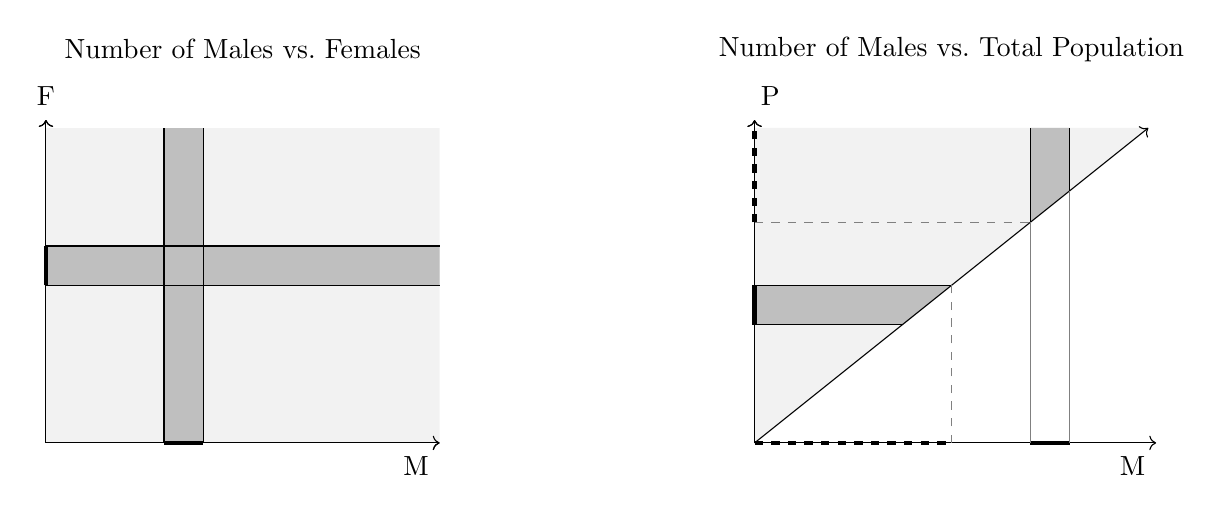
\begin{tikzpicture}
		\draw[->] (-1,3) -- (4,3);
		\draw[->] (-1,3) -- (-1,7.1);
		
		\node at (-1,7.4) {F};
		\node at (3.7,2.7) {M};
		
		\begin{scope}
			\clip (-1,3) rectangle (4,7);
			\fill[gray!10!white] (-1,3) rectangle (4,7);
		\end{scope}
		
		\begin{scope}
			\clip (-1,5) rectangle (4,5.5);
			\fill[gray!50!white] (-1,5) rectangle (4,5.5);
		\end{scope}
		
		\begin{scope}
			\clip (0.5,3) rectangle (1,7);
			\fill[gray!50!white] (0.5,3) rectangle (1,7);
		\end{scope}
		
		\begin{scope}
			\clip (0.5,5) rectangle (1,5.5);
			\fill[gray!50!white] (0.5,5) rectangle (1,5.5);
		\end{scope}
		
		\draw[black] (-1,5)--(4,5);
		\draw[black] (-1,5.5)--(4,5.5);
		
		\draw[black] (0.5,3) -- (0.5,7);
		\draw[black] (1,3) -- (1,7);
		
		
		\draw[->] (-1,3) -- (4,3);
		\draw[->] (-1,3) -- (-1,7.1);
		
		
		\draw[->] (8,3) -- (13.1,3);
		\draw[->] (8,3) -- (8,7.1);
		
		\draw[black,ultra thick] (-1,5) -- (-1,5.5);
		\draw[black,ultra thick] (0.5,3) -- (1,3);
		
		\node at (12.8,2.7) {M};
		\node at (8.2,7.4) {P};
		
		\begin{scope}
			\clip (8,3) -- (8,4.5) -- (9.89,4.5) -- (8,3);
			\fill[gray!10!white] (8,3) -- (8,4.5) -- (9.89,4.5) -- (8,3);
		\end{scope}
		\begin{scope}
			\clip (8,5) -- (10.5,5) -- (13,7) -- (8,7) -- (8,5);
			\fill[gray!10!white] (8,5) -- (10.5,5) -- (13,7) -- (8,7) -- (8,5);
		\end{scope}
		
		\begin{scope}
			\clip (8,4.5) -- (8,5) -- (10.5,5) -- (9.8,4.5) -- (8,4.5);
			\fill[gray!10!white] (8,4.5) -- (8,5) -- (10.5,5) -- (9.8,4.5) -- (8,4.5);
		\end{scope}
		
		\draw[->] (8,3) -- (8,7.1);
		
		
		\begin{scope}
			\clip (8,4.5) -- (8,5) -- (10.5,5) -- (9.89,4.5) -- (8,4.5);
			\fill[gray!50!white] (8,4.5) -- (8,5) -- (10.5,5) -- (9.89,4.5) -- (8,4.5);
		\end{scope}
		\begin{scope}
			\clip (11.5,5.8) -- (11.5,7) -- (12,7) -- (12,6.2) -- (11.5,5.8);
			\fill[gray!50!white] (11.5,5.8) -- (11.5,7) -- (12,7) -- (12,6.2) -- (11.5,5.8);
		\end{scope}
	
		\draw[->] (8,3) -- (13,7);
		
		\draw[black] (8,4.5) -- (9.89,4.5);
		\draw[black] (8,5) -- (10.5,5);	
		
		\draw[black, ultra thick, dashed] (8,3) -- (10.5,3);	
		\draw[black,ultra thick] (8,4.5) -- (8,5);
		
		\draw[gray,dashed] (10.5,3) -- (10.5,5);
		
		\draw[gray,dashed] (8,5.8) -- (11.5,5.8);
		
		\draw[black,ultra thick] (11.5,3) -- (12,3);
		\draw[black,ultra thick,dashed] (8,5.8) -- (8,7);
		
		\draw[gray] (11.5,3) -- (11.5,5.8);
		\draw[gray] (12,3) -- (12,6.2); 
		\draw[black] (11.5,5.8) -- (11.5,7);
		\draw[black] (12,6.2) -- (12,7);
		
		
		\node at (1.5,8) {Number of Males vs.~Females};
		\node at (10.5,8) { Number of Males vs.~Total Population};
\end{tikzpicture}
	\caption{Domain independence and projections. Given a population, the number of male and female members form independent domains: knowing something about one value tells us nothing about the other. Pictorially, a constraint on one side gives us a vertical or horizontal band, which projected on the other axis, gives us the full axis (i.e.~the certainty). On the other hand, the total population and the number of males are not independent domains: given the total population, the number of males cannot exceed that number; given the number of males, the total population cannot be lower than that number. Pictorially, we see that the combined domain does not span the whole plane. A constraint on one domain gives us, when projected, a constraint on the other domain.} \label{fig:2_relationships}
\end{figure}



\begin{mathSection}
	\begin{defn}
		The experimental domains of a countable set $\{\edomain_{X_i}\}_{i=1}^{\infty}$ are \textbf{independent} if taking one verifiable statement $\stmt_i \in \edomain_{X_i}$ from each domain always gives an independent set of statements.
	\end{defn}
	\begin{prop}
		Let $\{\edomain_{X_i}\}_{i=1}^{\infty}$ be a countable set of independent experimental domains and $X_i$ their respective possibilities. The set of possibilities $X$ of the combined experimental domain $\bigtimes\limits_{i=1}^{\infty} \edomain_{X_i}$ consists of all the possible conjunctions of the possibilities of each domain. That is: $X = \{ \bigAND\limits_{i=1}^{\infty} x_i \, | \, x_i \in X_i \}$. Notationally, we write $\edomain_X=\edomain_{\bigtimes\limits_{i=1}^{\infty} X_i}$.
	\end{prop}
	\begin{proof}
		A possibility $x \equiv \bigAND\limits_{i=1}^{\infty}x_i$ for the combined domain is the conjunction of possibilities of each individual domain by \ref{prop_combined_possibility}. Since the domains are independent and since possibilities are neither certainties nor impossibilities, by \ref{def_independent_statements} there exists an assignment $a \in \pAss$ such that $a(x_i) = \TRUE$ for all $i=1..\infty$ and therefore $a(x)=\TRUE$. That is, each conjunction $x=\bigAND\limits_{i=1}^{\infty}x_i$ is not impossible and therefore is a possibility.
	\end{proof}
	\begin{defn}
		Let $\{(X_i, \mathsf{T}_i)\}_{i=1}^{\infty}$ be a countable set of topological spaces. Let $X=\bigtimes\limits_{i=1}^{\infty} X_i$ be the Cartesian product of the points. Let $\mathcal{B}$ be the collection of sets of the form $\bigtimes\limits_{i=1}^{\infty} U_{i}$, with $U_i \in \mathsf{T}_i$ and $U_i \neq X_i$ only finitely many times. The topology generated by $\mathcal{B}$ is called the \textbf{product topology}.
	\end{defn}
	\begin{prop}
		Let $\{\edomain_{X_i}\}_{i=1}^{\infty}$ be a countable set of independent experimental domains. The natural topology for the possibilities of the combined experimental domain $\edomain_{\bigtimes\limits_{i=1}^{\infty} X_i}$ is the product topology of the natural topology for the possibilities of each domain.
	\end{prop}
	\begin{proof}
		Let $U_i : \edomain_{X_i} \to \mathsf{T}_{X_i}$ be the map from a verifiable statement of a domain to its verifiable set in the respective topology. Let $U : \edomain_{X} \to \mathsf{T}_X$ be the same map for the combined domain. Let $\stmt_i \in \edomain_{X_i}$ be a verifiable statement from a particular domain and $U_i(\stmt_i)$ its verifiable set in that domain. Since we also have $\stmt_i \in \edomain_{X}$, the statement is also associated with the verifiable set $U(\stmt_i)$ in the combined domain. Because the domains are independent, every possibility in $U_i(\stmt_i)$ is compatible with any possibility $x_j \in X_j$ for all $j \neq i$. This means that $U(\stmt_i)=X_1\times ... \times X_{i-1} \times U_i(\stmt_i) \times X_{i+1} \times ...$ . Given that a verifiable statement in the combined domain can be generated using finite conjunction and countable disjunction from the verifiable statements of the independent domains, the topology of the combined space can be generated by all sets of the form $\bigtimes\limits_{i=1}^{\infty} U_{i}$, with $U_i \in \mathsf{T}_i$ and $U_i \neq X_i$ only once. Using finite conjunction, this includes those sets where $U_i \neq X_i$ finitely many times. The natural topology of the combined domain is the product topology by definition.
	\end{proof}
\end{mathSection}

\subsection{Dependent domains}

Another special case is combining a domain $\edomain_X$ with another $\edomain_Y \subseteq \edomain_X$ that is dependent on it. For example, combining the domain for the temperature of a mercury column with the domain for its height. Since the height can be determined by the temperature, no new possibilities are added. The combined domain is equivalent to the independent domain $\edomain_X$ since all the verifiable statements in $\edomain_Y$ have equivalents in it.

\begin{mathSection}
	\begin{prop}
		Let $\edomain_X$ and $\edomain_Y$ be two experimental domains such that $\edomain_Y \subseteq \edomain_X$ depends on the first. Then $\edomain_X \times \edomain_Y \equiv \edomain_X$.
	\end{prop}
	\begin{proof}
		Since $\edomain_Y$ is dependent on $\edomain_X$, any statement in $\edomain_Y$ is equivalent to one in $\edomain_X$. Therefore no statement can be generated from them that is not equivalent to one already contained in $\edomain_X$. Therefore $\edomain_X \times \edomain_Y$ is equivalent to $\edomain_X$. 
	\end{proof}
	\begin{coro}
		Let $\edomain_X$ and $\edomain_Y$ be two experimental domains such that $\edomain_Y \subseteq \edomain_X$ depends on the first. The possibilities of $\edomain_X \times \edomain_Y$ are the possibilities of $\edomain_X$.
	\end{coro}
	\begin{proof}
		The possibilities of $\edomain_X \times \edomain_Y$ are the possibilities of $\edomain_X$ since they are equivalent domains. To be consistent with \ref{prop_combined_possibility}, we additionally show that they are also the subset of the Cartesian product. Let $f : X \to Y$ be the causal relationship between the domains, let $x$ and $y$ be two possibilities of the respective domains. We have $x \AND y \nequiv \impossibility$ if and only if $y = f(x)$, so the possibilities of $\edomain_X \times \edomain_Y$ are $x \AND f(x)$ for all $x \in X$. We also have $x \AND f(x) \equiv x$ since $x \narrower f(x)$.
	\end{proof}
\end{mathSection}


\subsection{Incompatible domains}

The last special case we consider is when the domains are incompatible, that is all verifiable statements of one are incompatible with the verifiable statements of the others. This is one case where the residual possibility behaves differently from all the others.\footnote{In fact, this is what prompted us to introduce the residual possibility.} Suppose $\edomain_X$ is the domain to classify a particular specimen as an animal and $\edomain_Y$ is the domain to classify it as a plant. If we take a verifiable statement from the first, such as \statement{that specimen has fur}, then it will be incompatible with a verifiable statement from the other, such as \statement{that specimen has lobed leaves}. The only way we can combine the possibilities is to take an established possibility of one (e.g. \statement{this specimen is a cat}) and combine it with the residual possibility of the other (e.g. \statement{this specimen is not a plant}). In other words, the combined possibilities are the union of the possibilities of the two domains (e.g. all possible plants and all possible animals).

In terms of the topology, the established possibilities of the combined domain are the disjoint union of the established possibilities of the original domains and their natural topology is the disjoint union topology (or co-product topology). 

\begin{mathSection}
	\begin{defn}
		Two experimental domains $\edomain_X$ and $\edomain_Y$ are \textbf{incompatible} if all verifiable statements in one are incompatible with all verifiable statements of the other. Formally, $\stmt_X \ncomp \stmt_Y$ for each pair of verifiable statements $\stmt_X \in \edomain_X$ and $\stmt_Y \in \edomain_Y$.
	\end{defn}
	\begin{coro}
		Let $\edomain_X$ and $\edomain_Y$ be two incompatible experimental domains. Then they must be incomplete and admit a residual possibility.
	\end{coro}
	\begin{proof}
		Let $\basis_X$ and $\basis_Y$ be a countable basis for the respective domain. Since we have $\stmt[e]_X \ncomp \stmt[e]_Y$ for all choices of $\stmt[e]_X \in \basis_X$ and $\stmt[e]_Y \in \basis_Y$, we also must have $\bigOR\limits_{\stmt[e]_X \in \basis_X} \stmt[e]_X \ncomp \bigOR\limits_{\stmt[e]_Y \in \basis_Y} \stmt[e]_Y$. Therefore $\bigOR\limits_{\stmt[e]_X \in \basis_X} \stmt[e]_X \nequiv \certainty$. Which means the residual possibility $\mathring{x} = \bigAND\limits_{\stmt[e]_X \in \basis_X} \NOT\stmt[e]_X = \NOT \bigOR\limits_{\stmt[e]_X \in \basis_X} \stmt[e]_X \nequiv \impossibility$. Therefore $\edomain_X$ is not complete and, by symmetry, neither is $\edomain_Y$.
	\end{proof}
	\begin{prop}
		Let $\{\edomain_{X_i}\}_{i=1}^{\infty}$ be a countable set of experimental domains pair-wise incompatible and $\dot{X}_i$ their respective established possibilities. The set of established possibilities $\dot{X}$ of the combined experimental domain $\bigtimes\limits_{i=1}^{\infty} \edomain_{X_i}$ consists of the disjoint union of the possibilities of each domain. That is: $\dot{X} = \coprod\limits_{i=1}^{\infty} \dot{X}_i = \bigcup\limits_{i=1}^{\infty} \dot{X}_i$ as $\dot{X}_i \cap \dot{X}_j = \emptyset$ for all $i,j \geq 1$ and $i \neq j$. Notationally, we write $\edomain_X=\edomain_{\coprod\limits_{i=1}^{\infty} X_i}$.
	\end{prop}
	\begin{proof}
		Consider two incompatible domains $\edomain_X$ and $\edomain_Y$. Let $\dot{x} \in X$ and $\dot{y} \in Y$ be two established possibilities. Then they both correspond to a minterm of the respective basis where at least one element is taken without negation. This also means that their conjunction will include the conjunction of one element of each of the basis. Since the elements of one basis are incompatible with the elements of the other, we have $\dot{x} \ncomp \dot{y}$.
		
		Now let $\dot{x} \in X$ be an established possibility, $\mathring{y} \in Y$ the residual and $\dot{Y} = Y \setminus \{\mathring{y}\}$ the established possibilities. We have $\dot{x} \equiv \dot{x} \AND \certainty \equiv \dot{x} \AND \bigOR\limits_{y \in Y} y \equiv \dot{x} \AND (\bigOR\limits_{\dot{y} \in \dot{Y}} \dot{y} \OR \mathring{y}) \equiv \bigOR\limits_{\dot{y} \in \dot{Y}} (\dot{x} \AND \dot{y}) \OR (\dot{x} \AND \mathring{y}) \equiv \impossibility \OR (\dot{x} \AND \mathring{y}) \equiv \dot{x} \AND \mathring{y}$. By symmetry, $\dot{y} \equiv \mathring{x} \AND \dot{y}$.
		
		To conclude, let $\mathring{x} \in X$ and $\mathring{y} \in Y$ be the two residual possibilities. The conjunction $\mathring{x} \AND \mathring{y}$ corresponds to a minterm where all the elements of the basis are negated. Therefore $\mathring{x} \AND \mathring{y}$ is the residual possibility of the combined domain, if it is not impossible. 
		
		Generalizing to a countable set of incompatible domains, the conjunction of all the residual possibilities $\mathring{x}= \bigAND_{i=1}^{\infty} \mathring{x}_i$ is the residual possibility of the combined domain, if it is not impossible. The only other conjunctions of the form $x= \bigAND_{i=1}^{\infty} x_i$ with $x_i \in X_i$ for all $i \geq 1$ that are not impossible are those where only one element is not a residual possibility. Those correspond to the established possibilities. But each of those conjunctions will be equivalent to the only element that is not a residual possibility. Therefore each established possibility of the combined domain is equivalent to an established possibility of one of the original domains: $\dot{X} = \bigcup\limits_{i=1}^{\infty} \dot{X}_i$. Given that the established possibilities of two incompatible domains are incompatible and therefore different, we have $\dot{X}_i \cap \dot{X}_j = \emptyset$ for all $i,j \geq 1$ and $i \neq j$. The established possibilities of the combined domains are the disjoint union of the established possibilities of the individual domains.
	\end{proof}

	\begin{defn}
		Let $\{(X_i, \mathsf{T}_i)\}_{i=1}^{\infty}$ be a countable set of topological spaces. Let $X=\coprod\limits_{i=1}^{\infty} X_i$ be the disjoint union of the points. The \textbf{disjoint union topology} $\mathsf{T}$ is the topology for which $U \in \mathsf{T}$ if and only if $U \cap X_i \in \mathsf{T}_i$ for all $i \geq 1$.
	\end{defn}

	\begin{prop}\label{prop_disjoint_union_topology_is_closure}
		The disjoint union topology is generated by closing the topologies of the initial spaces under disjoint union.
	\end{prop}
    \begin{proof}
		First we show that all disjoint unions of verifiable sets are part of the disjoint union topology. Let $\{(X_i, \mathsf{T}_i)\}_{i=1}^{\infty}$ be a countable set of topological spaces and $(X, \mathsf{T})$ their disjoint union with the disjoint union topology. Any disjoint union of verifiable sets can be put in the form $U=\coprod\limits_{i=1}^{\infty} U_i$ with $U_i \in \mathsf{T}_i$ for all $i \geq 1$. We have $U \cap X_i = \coprod\limits_{i=j}^{\infty} U_j \cap X_i = U_i$ for all $i \geq 1$. Therefore $U \in \mathsf{T}$ by definition.
		
		Now we show that any set in the disjoint union topology is the disjoint union of verifiable sets of the individual topologies. Let $U \in \mathsf{T}$. Since $U \subseteq X$ and $X$ is the disjoint union for all $X_i$, we can write $U=\coprod\limits_{i=1}^{\infty} U_i$. As before $U \cap X_i = U_i$ for all $i \geq 1$ and, since $U \cap X_i \in \mathsf{T}_i$ for all $i \geq 1$ by definition of the disjoint union topology, $U_i \in \mathsf{T}_i$ for all $i \geq 1$. Therefore any $U \in \mathsf{T}$ is the disjoint union of verifiable sets.
		
		This also shows that the disjoint union topology is a topology since it is closed under arbitrary union by definition, it is closed under finite intersection within each topology and it is closed under finite intersection across topologies since their intersection is always the empty set.
    \end{proof}

	\begin{prop}
		Let $\{\edomain_{X_i}\}_{i=1}^{\infty}$ be a countable set of pair-wise incompatible domains. The natural topology for the established possibilities of the combined experimental domain $\edomain_{\coprod\limits_{i=1}^{\infty} X_i}$ is the disjoint union topology of the natural topology for the established possibilities of each domain.
	\end{prop}
	\begin{proof}
		Given that the domains are incompatible, they are also incomplete. The only statement in each domain $\edomain_{X_i}$ compatible with the respective residual possibility $\mathring{x}_i$ will be the certainty $\certainty$. This means the natural topology restricted to the established possibilities contains all the verifiable sets associated to the impossibilities and to all verifiable statements. This will also be true for the combined domain $\edomain_{\coprod\limits_{i=1}^{\infty} X_i}$, if it is incomplete. If it is complete, then the established possibilities are the full possibilities and their natural topology coincides. Note that all verifiable statements in the combined domain can be generated from the verifiable statements of the individual domains. Also note that the conjunction between the different domains is an impossibility and therefore does not yield a new statement. Therefore all the statements whose verifiable sets form the topology on the established possibilities on the combined domain can be generated by the disjunction of all the statements whose verifiable sets form  the topology on the established possibilities on the individual domains. Therefore the topology of the combined space is simply closing the individual topologies under the disjoint union. The topology of the combined space is therefore the disjoint union topology by \ref{prop_disjoint_union_topology_is_closure}
	\end{proof}
\end{mathSection}

For topologies, as well as for other mathematical structures, we can choose between two types of products. If we have two one dimensional euclidean spaces we can decide whether to take their product (i.e. the plane) or their co-product (i.e. the disjoint union of the two lines). For experimental domains we do not choose: it is what it is. There is no way to combine the two experimental domains for temperature and height of the same mercury column and get the Cartesian product of their possibilities. Though combining two independent domains mimics the categorical product and combining two incompatible domains mimics the categorical co-product, it is the semantic (and ultimately physical) relationship between them that decides which product we have. This is another case where the mathematical structures ``forget" the full equivalence. The topology only captures how the temperature and height can be measured, and not whether they are independent, dependent or incompatible. That information lies outside of the topology and therefore needs to be added by choosing the correct combination.

\section{Experimental domain for experimental relationships}

Now that we have seen how to describe relationships between domains, we should ask: are experimental relationships themselves something we can experimentally verify? We may know that there is a relationship between the temperature of a mercury column and its height, but how can we confirm experimentally which one it is?

The main result of this section is to show that, given two related experimental domains, we can always mathematically construct from them another experimental domain for which the possibilities are continuous functions between the possibilities of the original domains. This means that, since we can recursively create relationship domains about relationship domains, the universe of discourse of our mathematical framework is closed. Yet, the availability of the experimental tests (i.e. whether the statements we construct are actually verifiable) is not guaranteed.

First of all we have to clarify within our framework what it means to experimentally verify a relationship. Suppose $\edomain_X$ is the domain for the state of a light switch, up or down being the two possibilities, and $\edomain_Y$ is the domain for the state of the light, which can be on or off. Suppose we could have three cases: the one where the switch is wired correctly, up corresponding to on, the one where the switch is wired incorrectly, up corresponding to off, and the one where the switch is not actually wired to the light, the two domains are independent. Each of these cases is represented by a different set of logical relationships, a different set of possible assignments.

\begin{table}[h]
\centering
\begin{tabular}{c|c|c|c}
\multicolumn{2}{c|}{X} & \multicolumn{2}{c}{Y} \\
	up & down & on & off \\
	\hline
	T & F & T & F \\
	F & T & F & T \\
\end{tabular}
\caption{Case 1: switch wired correctly to the light}
\end{table}

\begin{table}[h]
\centering
\begin{tabular}{c|c|c|c}
	\multicolumn{2}{c|}{X} & \multicolumn{2}{c}{Y} \\
	up & down & on & off \\
	\hline
	T & F & F & T \\
	F & T & T & F \\
\end{tabular}
\caption{Case 2: switch wired incorrectly to the light}
\end{table}

\begin{table}[h]
	\centering
	\begin{tabular}{c|c|c|c}
		\multicolumn{2}{c|}{X} & \multicolumn{2}{c}{Y} \\
		up & down & on & off \\
		\hline
		T & F & T & F \\
		T & F & F & T \\
		F & T & T & F \\
		F & T & F & T \\
	\end{tabular}
	\caption{Case 3: switch not wired to the light}
\end{table}

Each case, then, is a different model: a different logical context. To experimentally verify which model is the right one means verifying statements of the type \statement{it is possible for the switch to be up while the light is on}. This does not correspond to \statement{the switch is up} $\AND$ \statement{the light is on} but to \statement{the switch is up} $\comp$ \statement{the light is on}. These are statements about the table and they cannot be columns of the table itself. What we need to create is a metacontext, in which each line corresponds to one choice of model, to one context.

\begin{table}[h]
	\centering
	\begin{tabular}{r|c|c|c|c}
		& up $\comp$ on & down $\comp$ on & up $\comp$ off & down $\comp$ off \\
		\hline
		Case 1 & T & F & F & T \\
		Case 2 & F & T & T & F \\
		Case 3 & T & T & T & T \\
	\end{tabular}
	\caption{Possible assignments for the metacontext}
\end{table}

Each line will tell us what statements are compatible and given the truth values of the line we can reconstruct the model. The verifiable statements that distinguish between different models, therefore, live in this metacontext and so will the experimental domain for the relationships.

\begin{mathSection}
	\begin{defn}
		Let $\logCtx_1$ and $\logCtx_2$ be two logical contexts. Let $S_1 \subseteq \logCtx_1$ and $S_2 \subseteq \logCtx_2$ be sets of statements. We say $f : S_1 \to S_2$ is a \textbf{logic homomorphism} if it preserves the logical structure. That is:
		\begin{itemize}
			\item possible assignments on $S_2$ correspond to possible assignments on $S_1$: if $a_2 \in \pAss[S_2]$ then there exists $a_1 \in \pAss[S_1]$ such that $a_1(\stmt) = a_2(f(\stmt))$ for all $\stmt \in S_1$
			\item a verifiable statement of $S_1$ is mapped to a verifiable statement in $S_2$
		\end{itemize}
		Additionally, if there exists a logic homomorphism $g : S_2 \to S_1$ such that $f \circ g = \Id_{S_1}$ and $g \circ f = \Id_{S_2}$ then $f$ is a \textbf{logic isomorphism} and $g$ is the \textbf{inverse} of $f$. Two logic isomorphisms $f : S_1 \to S_2$ and $g : S_1 \to S_2$ are equivalent if $f(\stmt)\equiv g(\stmt)$ for all $\stmt \in S_1$.
	\end{defn}

\begin{coro}\label{3_coro_logic_homomorphism_preserves_boolean}
	Let $h : S_1 \to S_2$ be a logic homomorphism, then for every $\hat{\stmt} \in S_1$, $\hat{S} \subseteq S_1$ and $f_\Bool : \Bool^{\hat{S}} \to \Bool$ such that $a_1(\hat{\stmt}) = f_\Bool(\{ a_1(\stmt) \}_{\stmt \in \hat{S}})$ for all $a_1 \in \pAss[S_1]$, then $a_2(h(\hat{\stmt})) = f_\Bool(\{ a_2(h(\stmt)) \}_{\stmt \in \hat{S}})$ for all $a_2 \in \pAss[S_2]$. In particular:
	\begin{itemize}
		\item $h(\NOT \stmt) \equiv \NOT h(\stmt)$ for all $\stmt \in S_1$
		\item $h(\bigAND_{\stmt \in S} \stmt) \equiv \bigAND_{\stmt \in S} h(\stmt)$ for all $S \subseteq S_1$
		\item $h(\bigOR_{\stmt \in S} \stmt) \equiv \bigOR_{\stmt \in S} h(\stmt)$ for all $S \subseteq S_1$
	\end{itemize}
\end{coro}

\begin{proof}
	If $a_1(\hat{\stmt}) = f_\Bool(\{ a_1(\stmt) \}_{\stmt \in \hat{S}})$ for all $a_1 \in \pAss[S_1]$ then, by the first property of logic homomorphisms, there is no $a_2 \in \pAss[S_2]$ such that $a_2(h(\hat{\stmt})) \neq f_\Bool(\{ a_2(h(\stmt)) \}_{\stmt \in \hat{S}})$. Therefore $a_2(h(\hat{\stmt})) = f_\Bool(\{ a_2(h(\stmt)) \}_{\stmt \in \hat{S}})$ for all $a_2 \in \pAss[S_2]$.
	
	In particular, since the relationship holds for any arbitrary $f_\Bool$, it will hold for negation, arbitrary conjunction and arbitrary disjunction.
\end{proof}

\begin{prop}
	Let $\logCtx_1$ and $\logCtx_2$ be two logical contexts. Let $S_1 \subseteq \logCtx_1$ and $S_2 \subseteq \logCtx_2$ be sets of statements and $f : S_1 \to S_2$ a logic homomorphism. Let $\bar{S}_1 \subseteq \logCtx_1$ and $\bar{S}_2 \subseteq \logCtx_2$ be the closure of $S_1$ and $S_2$ respectively under arbitrary conjunction, arbitrary disjunction and negation. Then if there exists a logic homomorphism $\bar{f} : \bar{S}_1 \to \bar{S}_2$ such that $\bar{f}(\stmt_1) \equiv f(\stmt_1)$ for all $\stmt_1 \in S_1$ it is unique.
\end{prop}

\begin{proof}
	Let $\tstmt_1 \in \bar{S}_1$ but $\tstmt_1 \notin S_1$. Then $\tstmt_1$ depends on $S_1$ through some $g_\Bool : \Bool^{S_1} \to \Bool$. Let $\bar{f}_1 : \bar{S}_1 \to \bar{S}_2$ and $\bar{f}_2 : \bar{S}_1 \to \bar{S}_2$ be two logic homomorphisms such that $\bar{f}_1(\stmt_1) \equiv \bar{f}_2(\stmt_1) \equiv f(\stmt_1)$ for all $\stmt_1 \in S_1$. Then by \ref{3_coro_logic_homomorphism_preserves_boolean} both $\bar{f}_1(\tstmt_1)$ and $\bar{f}_2(\tstmt_1)$ depend on $S_2$ through $g_\Bool$. This means that in every possible assignment $a \in \pAss[\bar{S}_2]$ we have $a(\bar{f}_1(\tstmt_1)) = a(\bar{f}_2(\tstmt_1))$  and therefore $\bar{f}_1(\tstmt_1) \equiv \bar{f}_2(\tstmt_1)$. Then $\bar{f}_1$ and $\bar{f}_2$ are equivalent.
\end{proof}


\begin{defn}
	Let $\edomain_X, \edomain_Y \subseteq \logCtx$ be two experimental domains. The \textbf{relationship metacontext}  $\logCtx_{C(X,Y)}$ between $\edomain_X$ and $\edomain_Y$ over $\{ \logCtx_i \}_{i \in I}$ is defined by following construction. Let $I$ be an index set. Let $\{ \logCtx_i \}_{i \in I}$ be an indexed set of logical contexts, let $\{ \edomain_{X_i} \}_{i \in I}$ and $\{ \edomain_{Y_i} \}_{i \in I}$ be two indexed sets of experimental domains such that $\edomain_{X_i}, \edomain_{Y_i} \subseteq \logCtx_i$ for all $i \in I$. Let $\{f_{i}\}_{i \in I}$ be a set of logic isomorphisms such that $f_{i} : \edomain_{X} \to \edomain_{X_i}$. Let $\{g_{i}\}_{i \in I}$ be a set of logic isomorphisms such that $g_{i} : \edomain_{Y} \to \edomain_{Y_i}$.
	
	Let $S$ be the set of ordered pairs of $\edomain_{X}$ and $\edomain_{Y}$ and \statement{$\stmt_x \comp \stmt_y$} be the notation of an element of $S$ for some $\stmt_x \in \edomain_{X}$ and $\stmt_y \in \edomain_{Y}$. For each $i \in I$, let $a_i \in \Bool^S$ be such that  $a_i(``\stmt_x \comp \stmt_y") = \TRUE$ if and only if $f_{i}(\stmt_x) \comp g_{i}(\stmt_y)$. Define $\pAss = \{ a_i \, | \, \forall i \in I \}$. Assume $a_i \neq a_j$ if $i \neq j$; if not, given a subset of $I$ that leads to the same possible assignment, remove all elements but one. Pick $t \in I$ and define $\truth = a_t$.
	
	Given an arbitrary function $f_\Bool : \Bool^S \to \Bool$, we can extend the set $S$ with a new element for which the possible assignments are calculated according to the function. The relationship context $\logCtx_{C(X,Y)}$ is the closure of $S$ under all possible functions $f_\Bool \in \Bool^S$.
	
	Let $S_v \subseteq S$ be set of statements \statement{$\stmt_x \narrower \stmt_y$}=\statement{$\stmt_x \ncomp \NOT \stmt_y$}=$\NOT$\statement{$\stmt_x \comp \NOT \stmt_y$} such that $\stmt_x \in \edomain_{X}$ and $\stmt_y \in \edomain_{Y}$ are verifiable. The set of verifiable statements $\vstmtSet \subseteq \logCtx$ for the relationship context is the set of statements generated by $S_v$ using finite conjunction and countable disjunctions.
\end{defn}
\begin{justification}
	By constructions, the relationship context satisfies the axioms for a logical context. We have a set of elements and a set of possible assignments of which one is the truth, this satisfies axioms \ref{ax_statement} and \ref{ax_possible_assignemetns}. Some of the statements are verifiable and satisfy \ref{ax_verifiable_statements}. Closure for axioms \ref{ax_functions_of_statement}, \ref{ax_verifiable_AND} and \ref{ax_verifiable_OR} are satisfied by constructions. We need to clarify why and in what cases this construct makes physical sense.
	
	The set $\{ \logCtx_i \}_{i \in I}$ consists of different contexts, each containing a copy of the domains $\edomain_X$ and $\edomain_Y$ with a different relationship between them. For example, if $\edomain_X$ is the domain for a light switch, up or down being the possibilities, and $\edomain_Y$ is the domain for the light, being on or off, in one context the two domain may have a causal relationship (i.e. the switch is wired to the light), in another they may have a different causal relationship (i.e. the switch is wired in the wrong way), and in yet another they may be independent (i.e. switch is not wired with the light). The logic isomorphisms $\{f_{i}\}_{i \in I}$ and $\{g_{i}\}_{i \in I}$ allow us to relate the statements that represent the same  assertion in the different contexts.
	
	Note that while mathematically we can always construct the relationship metacontext, it may not exist in reality. Specifically, there is nothing that guarantees that statements of the form \statement{$\stmt_x \narrower \stmt_y$} are actually verifiable.
\end{justification}
\end{mathSection}

Now that we have the right context, we have to understand what is the right basis to generate the experimental domain. Suppose we have a way to verify experimentally statements of the type \statement{the temperature of the mercury column is between 24 and 25 Celsius}$\narrower$\statement{the height of the mercury column is between 24 and 25 millimeters}. That is, we can verify that whenever $\stmt_X=$\statement{the temperature of the mercury column is between 24 and 25 Celsius} is verified, then $\stmt_Y=$\statement{the height of the mercury column is between 24 and 25 millimeters} is verified. In that case, we can explore the connection between the two domains within different ranges at ever increasing precision. This means we can narrow the range of possible functions in the same way that we can narrow the range of possible values for a quantity. These types of statements, then, form an experimental domain where each possibility corresponds to a possible continuous function between the two initial experimental domains.

\begin{mathSection}
	\begin{defn}
		Let $\logCtx_{C(X,Y)}$ be the relationship metacontext between $\edomain_X$ and $\edomain_Y$ over $\{ \logCtx_i \}_{i \in I}$. Let $\edomain_{Y_i} \subseteq \edomain_{X_i}$ for all $i \in I$. Let $\basis_X \subseteq \edomain_X$,  $\basis_Y \subseteq \edomain_Y$ be the two countable basis of the respective domains and let $\basis = \{ ``\stmt[e]_x \narrower \stmt[e]_y" \, | \,  \stmt[e]_x \in \basis_X, \stmt[e]_y \in \basis_Y\}$. Then the \textbf{relationship domain} $\edomain_{C(X,Y)}$ is the experimental domain generated by $\basis$.
	\end{defn}
	\begin{proof}
		The only thing that needs to be checked is that the basis that generates $\edomain_{C(X,Y)}$ is countable. Since $\basis_X$ and $\basis_Y$ are countable, the set of statements of the form $\mathbin{\narrower}(\stmt[e]_x, \stmt[e]_y)$ with $\stmt[e]_x \in \basis_X$ and $ \stmt[e]_y \in \basis_Y$ is also countable.
	\end{proof}
\begin{prop}\label{2_prop_relationship_domain_is_space_of_continuous_functions}
	The possibilities for a relationship domain $\edomain_{C(X,Y)}$ coincide with the possible experimental relationships between $X$ and $Y$. That is, for each possibility $z$ of $\edomain_{C(X,Y)}$ there exists a continuous function $f_z : X \to Y$ such that $z\equiv\bigAND\limits_{x\in X} ``x \narrower f_z(x)"$ and an $i \in I$ such that $\bar{g}_i(f_z(\bar{f}_i^{-1}(x_i))) \equiv f_c (x_i)$ for all $x_i \in X_i$ where $f_c$ is the causal relationship between $\edomain_{X_i}$ and $\edomain_{Y_i}$.
\end{prop}
\begin{proof}
	First we show that for each possibility $z$ of the relationship domain there exists a set $P_z \subseteq X \times Y$ such that $z \equiv \bigAND\limits_{(x,y) \in P_z} ``x \comp y"  \AND \bigAND\limits_{(x,y) \nin P_z} ``x \ncomp y"$. Let $z$ be a possibility of a relationship domain. This will be a minterm of the basis therefore $z \equiv minterm(\basis)$. Let $x \in X$ and $y \in Y$ be two possibilities and consider the statement $``x \comp y"$. If $z$ is true in a possible assignment, then the truth value for all statements of the form $``e_x \narrower e_y"$ where $(e_x, e_y) \in \basis_X \times \basis_Y$ will be set. But $x \ncomp y$ if and only if there exists at least one pair $(e_x, e_y) \in \basis_X \times \basis_Y$ such that $x \narrower e_x \narrower e_y$ and $y \ncomp e_y$. Therefore if $z$ is true in an assignment it will tell us whether $x \ncomp y$ is true or not, so we either have $z \narrower ``x \comp y"$ or $z \narrower \NOT ``x \comp y"$. Let $P_z = \{ (x,y) \in X \times Y \, | \, z \narrower ``x \comp y" \}$ and $\hat{z} = \bigAND\limits_{(x,y) \in P_z} ``x \comp y" \AND  \bigAND\limits_{(x,y) \nin P_z} \NOT ``x \comp y" $. Then $z \narrower \hat{z}$.
	
	Conversely, if we suppose $\hat{z}$ to be true in an assignment, then we will know the truth assignment for all statements of the form $``x \comp y"$ where $(x,y) \in X \times Y$. Let $(e_x, e_y) \in \basis_X \times \basis_Y$ and consider the statement $``e_x \narrower e_y"$. We have $e_x \narrower e_y$ if and only if there is no pair $(x,y)$ such that $x \narrower e_x$, $y \ncomp e_y$ and $x \comp y$. Therefore if $\hat{z}$ is true in an assignment it will tell us whether $e_x \narrower e_y$ is true or not, so we either have $\hat{z} \narrower ``e_x \narrower e_y"$ or $\hat{z} \narrower \NOT ``e_x \narrower e_y"$. As $z$ is a minterm of statements of the form $``e_x \narrower e_y"$, we'll either have $\hat{z} \narrower z$ or $\hat{z} \ncomp z$. Since $z \narrower \hat{z}$,  $\hat{z} \comp z$ and therefore $\hat{z} \narrower z$. Since we also have $z \narrower \hat{z}$, then we have $z \equiv \hat{z}$.
	
	Now we want to show that for each possibility $z$ there is a function $f_z : X \to Y$ such that $z\equiv\bigAND\limits_{x\in X} ``x \narrower f_z(x)"$. We note that statements of the form $``\stmt_x \comp \stmt_y"$ are precisely the statements used to generate the relationship metacontext. Statements of the form $``x \comp y"$, where $x \in X$ and $y \in Y$, are enough to determine the truth value of statements of the form $``\stmt_x \comp \stmt_y"$. Therefore for each possibility $z$ there is one and only one possible truth assignment in which $z$ is true. That is, each $x$ correspond to particular logical context $\logCtx_i$. Since in that context $\edomain_{Y_i} \subseteq \edomain_{X_i}$ there will be a causal relationship $f_i : X_i \to Y_i$ such that $x_i \narrower f_i (x_i)$ which means $x_i \comp y_i$ if and only if $y_i = f_i(x_i)$. Since causal relationships are unique and the possible assignments are distinct, to each $z$ will correspond a unique $f_z : X \to Y$ such that $\bar{g}_i \circ f_z \circ \bar{f}^{-1}_i = f_i$ and $z\equiv\bigAND\limits_{x\in X} ``x \narrower f_z(x)"$. Moreover $f_z$ is continuous since $\bar{f}_i$ and $\bar{g}_i$ are logical isomorphisms.
\end{proof}
\end{mathSection}

Note that the definition for the metacontext simply declares some statements to be verifiable: it does not guarantee that this is actually possible. So when can we do it? Or better, what do we need in practice to be able to build the necessary confidence? Let's think how we would test the relationship between temperature and height of a mercury column. We would prepare different mercury samples with different values of temperatures in many different conditions, measure height and temperature with different devices, repeat many times, ask someone else to do it independently, compare results, and so on. At some point we will have explored enough of the possible cases, checked and tried anything that could invalidate the result and we will have the confidence to say that \statement{if the temperature of the mercury column is between 24 and 25 Celsius then its height is between 24 and 25 millimeters}. We should stress that the procedure is not at all to observe a few values and then generalize. It is not mere induction. It is the ability to prepare and control the system in many different conditions and our inability to violate the relationship that gives us the confidence needed to reach the conclusion.

Suppose, in fact, that we want to experimentally verify the link between inflation and money supply. As long as we cannot create new countries in different economic conditions, the only thing we can do is gather data for as many nations as we can throughout history.\footnote{Computer simulations can sometimes alleviate this problem, though they are only as good as the model one uses.} Since we cannot purposely explore different conditions and we can't even replicate older ones, the best we can do is show that there was a correlation between those specific values. It is the inability to freely and fully explore the problem space that may not enable us to experimentally verify the causal relationship.\footnote{In this sense, experimental sciences allow for more rigorous results than observational sciences precisely because it is more feasible to experimentally test relationships between domains.}

The point is that we cannot give a general purpose algorithm for how to construct experimental tests for the relationships starting from the experimental tests of the individual domains. We cannot formalize in general what it means that we have explored the space ``enough" to consider the relationship verified, no more than we can formalize when the data collected is ``enough" to consider a statement verified or when a statement is specific ``enough" to consider the semantics well defined. This is where the practice of experimental science comes in.

But, while we may not know in general whether we can experimentally verify a relationship between two specific domains, we do know that the relationship domain can always be constructed in principle and therefore our mathematical framework is complete. That is: we can take two experimental domains (e.g. $\edomain_t$ for time and $\edomain_x$ for position), construct a relationship domain between them (e.g. $\edomain_{x(t)}$ for trajectories in space), then take another experimental domain (e.g. $\edomain_{(q,p)}$ for the states) and construct another relationship domain between the two (e.g. $\edomain_{(q,p)\to x(t)}$ for the relationship between states and trajectories). Our general mathematical theory of experimental science is therefore closed, since we can recursively create relationship domains about relationship domains indefinitely while remaining within its bounds. In other words, experimentally distinguishable objects and their relationships will never lie outside of the theory.


\section{Summary}

In this chapter we have seen the first important set of consequences of our general mathematical theory of experimental science. We have seen that experimental relationships between domains can be defined in terms of inference between verifiable statements or equivalently in terms of causal relationship between possibilities. The causal relationship always corresponds to a continuous function in the natural topology. Moreover, it will need to preserve any additional mathematical structure that formalizes a physical characteristic of the domain.

We have also seen how to combine a set of countably many experimental domains and how the combined possibilities depend on the logical and semantic relationships that exist across domains. Depending on the case, we can have the Cartesian product of the possibilities (with the product topology) all the way to the disjoint union of the established possibilities (with the disjoint union topology).

We have shown that it is possible to construct experimental domains for the relationships themselves. This means that within our theory we can describe relationships of arbitrarily higher order (i.e. relationships about relationships) and therefore we never go outside of our framework.

As we have only explored simple constructions based on the original concepts, these conclusions are of a general nature and therefore must apply to any area of science. 

\chapter{Properties and quantities}

In this chapter we will introduce the idea of \textbf{properties}, which we use to label the possibilities of an experimental domain. For example, we may use names to distinguish among people, fur color to distinguish among cats, pressure to distinguish the state of a gas. In particular, we'll define a \textbf{quantity} as a property that has a magnitude: we can compare two different values and determine which one is greater or smaller.

Instead of simply assuming we have quantities, we will need to construct them from the verifiable statements of an experimental domain. To do that, we will prove three theorems that will give necessary and sufficient conditions for that construction, clarifying how quantities are defined experimentally. These theorems will allow us to understand how the ordering of the values for a quantity are linked to the logical relationships between the verifiable statements, and in particular how the ordering of values is linked to the ordering defined by narrowness.

After characterizing quantities in general, we will see the cases of \textbf{discrete} and \textbf{continuous} quantities. We will see how discrete quantities are linked to decidability, the ability to verify both a statement and its negation, while continuous quantities are linked to a lack thereof. We will then discuss how the requirements for continuous quantities cannot be truly realized in practice and what happens when that idealization fails.

\section{Properties}

Whether the result of direct observation or not, a physical object is most often identified by its properties and their values. A person may be identified by name and date of birth; a bird may be characterized by the color of its beak; the state of a particle may be qualified by its position and momentum.

In this section we define how in general we can use properties to label the possibilities of an experimental domain. Each property will specify a continuous function from the possibilities to the topological space of the possible property values. Some properties may fully identify each possibility, as they assign distinct values, and some may also fully characterize which statements are verifiable.

Suppose $\edomain_X$ is a domain for animal identification and $X$, its possibilities, are all animal species. Providing good names and definitions for species is a whole scientific subject by itself (i.e. taxonomy) with its own rules (i.e. the International Code of Zoological Nomenclature). The ICZN assigns each species a name composed of two Latin words. For example, \statement{Passer domesticus} is the official name for the house sparrow while \statement{Passer italiae} is the one for the Italian sparrow. This means that identifying an animal species is equivalent to identifying its name. Therefore the domain to identify the species name $\edomain_{\mathcal{Q}} \equiv \edomain_X$ is equivalent to the one for identifying the actual species and we have an experimental relationship $q: X \to \mathcal{Q}$ between them. As each species is given a unique name this is the most discriminating type of property: one that covers the whole range of possibilities and fully identifies each of them. But this is a special case.

The ICZN also assigns a genus (pl. genera) to each species, which corresponds to the first part of the species name. For example, both aforementioned sparrows are of the genus \statement{Passer} while all swans, black or white, are of the genus \statement{Cygnus}. Now suppose that $\mathcal{Q}$ is the set of all names for all genera and $q: X \to \mathcal{Q}$ is the function that gives us the genus name for each species. We can still use this as a label for our possibilities, but it does not fully identify them.

On a different note, we could decide to distinguish species by their morphological attributes. For example, if $\mathcal{Q}$ is the set of all colors, we can imagine a function that gives us the beak color for each species. The function is partial, not defined on all elements, as not all species have a beak or its color may not be unique. We have $q: U \to \mathcal{Q}$ where $U \subseteq X$ is the set where the property is defined. To be consistent, though, we must at least be able to tell in what cases the property is actually defined. For example, we must be able to tell whether an animal has a beak. Therefore there must be a verifiable statement that is true if and only if the property is well defined. The set $U$, then, must correspond to the verifiable set of said statement.

Other examples of properties include: postal addresses for buildings, tax ID numbers for people, generation for fundamental particles, position of the center of mass of a body. In all these cases, the general pattern is that we assign a label to a possibility from an established set.

\begin{mathSection}
	\begin{defn}
		A \textbf{property} for an experimental domain $\edomain_X$ is any attribute we can use to distinguish between its possibilities. Formally, it is a tuple $(\mathcal{Q}, q)$ where $\mathcal{Q}$ is a topological space and $q : U \to \mathcal{Q}$ is a continuous function where $U \in \mathsf{T}_X$ is a verifiable set of possibilities.
	\end{defn}
	\begin{justification}
		Suppose $q$ is a physical property that can be assigned to distinguish the set of possibilities $U \subseteq X$. We must be able to tell experimentally whether the property is defined for each possibility. Therefore we are justified to assume that $U$ is a verifiable set. Let $\mathcal{Q}$ be the set of possible values for the property. Each element of $U$ will be matched with a possible value. Therefore we are justified to assume there is a function $q : U \to \mathcal{Q}$ that specifies that mapping.
		
		As we must be able to experimentally distinguish between the values in $\mathcal{Q}$, there must be a collection $\mathsf{T}_Q$ of verifiable sets that corresponds to the possible verifiable statements associated to the quantity. Therefore we are justified to assume $\mathcal{Q}$ is a topological space. Moreover, since the property value is determined by each possibility, the function $q$ establishes a causal relationship between the two and therefore we are justified to assume $q$ is a continuous function.
	\end{justification}
\end{mathSection}
		
Note that we have not defined a property as an experimental domain. The possibility of the domain for a property would be a statement like \statement{the species name for this animal is Passer domesticus} while the value is just the object \statement{Passer domesticus}. The idea is that the property and its values are defined independently of the particular object. For example, distance in meters is defined independently of whether we later want to measure the earth diameter or its distance to the moon.\footnote{While in principle we could envision a formal construction of properties and their values purely built on top of the notion of statement (e.g. define the value \emph{red} to be the set of all statements that claim that something is of that color) we are not going to do so. While appealing in some respects, it is not clear whether such a construction would actually help to clarify underlying assumptions while it is clear it would distract from other more critical issues.}

The fact that the property and its values are defined more generally leads to some subtle issues: even if each possibility of the domain corresponds to one property value and each verifiable statement of the property is equivalent to a verifiable statement of the domain, the reverse may not be true. Consider the experimental domain for identifying negatively charged fundamental particles. In this case, each particle will correspond to a unique value of mass, and by measuring the mass we can infer the particle. But for each possible value of mass we will not have a possible fundamental particle. Moreover, the verifiable statement \statement{this particle is an electron} would correspond to an infinitely precise statement of the form \statement{the mass of the particle is exactly 510998.9461... eV} which is not verifiable. The reason is that identifying a negatively charged particle is not the same as measuring its mass with arbitrary precision: in the first case we can stop when there is only one possible particle within the finite range of our measurement. Now consider the experimental domain for the position of the center of mass of a particle along a particular direction. Not only is the distance from a fixed point enough to identify the position, but for each value of the distance we also have a possible position of the particle.

We say that a property fully characterizes an experimental domain if each possible value of a property corresponds to a possibility of the domain, like in the case of the distance from a reference and position of a particle. The idea is that it tells us what cases are possible and how they are experimentally verified. Instead, we say that a property fully identifies an experimental domain if each possibility corresponds to a unique value, like in the case of the mass of a negatively charged particle. The idea is that the value of the property allows us to uniquely identify the possibility but nothing more.

\begin{mathSection}
	\begin{defn}
		The possibilities of an experimental domain are \textbf{fully identified} by a property if its value is enough to uniquely determine a possibility. Formally, let $(\mathcal{Q}, q)$ be a property for an experimental domain $\edomain_X$. Then the possibilities $X$ are fully identified if $q: X \to \mathcal{Q}$ is injective.
	\end{defn}
	
	\begin{defn}
		An experimental domain is \textbf{fully characterized} by a property if all verifiable statements in the domain correspond to verifiable statements on the property and vice-versa. Formally, let $(\mathcal{Q}, q)$ be a property for an experimental domain $\edomain_X$. Then it is fully characterized if $q: X \to \mathcal{Q}$ is a homeomorphism.
	\end{defn}
\end{mathSection}

\section{Quantities and ordering}

We now focus our attention on those properties that can be quantified. The number of people in a group can be quantified by an integer, the distance between two objects can be quantified in meters, the force acting on a body can be quantified by the magnitude of a vector expressed in Newtons. The defining characteristic for a quantity is that a value can be greater, smaller or equal to another.

In this section we will define a quantity as a property with a linear order which we assume given a priori, and study its relationship with the experimental domain. We will define the order topology, which assumes one can experimentally verify whether a value is before or after another one. We will see that a domain is fully characterized by a quantity only if the possibilities themselves can be ordered, and how this ordering, in the end, is uniquely characterized by statement narrowness: 10 is less than 42 because \statement{the quantity is less than 10} is narrower than \statement{the quantity is less than 42}.

As the defining characteristic for a quantity is the ability to compare its values, then the values must be ordered in some fashion from smaller to greater. Therefore, given two different values, one must be before the other. Mathematically, we call linear order an order with such a characteristic as we can imagine the elements positioned along a line. Note that vectors are not linearly ordered: no direction is greater than the other. Therefore, in this context, a vector will not strictly be a quantity but a collection of quantities.\footnote{In other languages, there are two words to differentiate quantity as in ``physical quantity" (e.g. grandezza, Gr\"osse, grandeur) and as in ``amount" (e.g. quantit\`a, Menge, quantit\'e). It is the second meaning of quantity that is captured here.}

We also have to define how this order can be experimentally verified. The idea is that we should, at least, be able to verify that the value of a given quantity is before or after a set value. This allows us to construct bounds such as \statement{the mass of the electron is $511 \pm 0.5$ keV} which we take to be equivalent to \statement{the mass of the electron is more than 510.5 keV but less than 511.5 keV}.\footnote{The sentence \statement{the mass of the electron is $511 \pm 0.5$ keV} could instead be referring to statistical uncertainty instead of an accuracy bound and would constitute a different statement when the different meaning is attached. We will be treating these types of statistical statements later in the book, but suffice it to say that they cannot be defined before statements that identify bounds.} For integers, this also allows us to verify particular numbers as \statement{the earth has one natural satellite} is equivalent to \statement{the earth has more than zero natural satellites and fewer than two}. Therefore we will define the order topology as the one generated by sets of the type $(a, \infty)$ and $(-\infty, b)$.

A quantity, then, is an ordered property with the order topology.

\begin{mathSection}
\begin{defn}
	A \textbf{linear order} on a set $\mathcal{Q}$ is a relationship $\leq : \mathcal{Q} \times \mathcal{Q} \to \mathbb{B}$ such that:
	\begin{enumerate}
		\item (antisymmetry) if $q_1 \leq q_2$ and $q_2 \leq q_1$ then $q_1 = q_2$
		\item (transitivity) if $q_1 \leq q_2$ and $q_2 \leq q_3$ then $q_1 \leq q_3$
		\item (total) at least $q_1 \leq q_2$ or $q_2 \leq q_1$
	\end{enumerate}
	A set together with a linear order is called a \textbf{linearly ordered set}.
\end{defn}
\begin{defn}
	Let $(\mathcal{Q}, \leq )$ be a linearly ordered set. The \textbf{order topology} is the topology generated by the collections of sets of the form:
	$$(a, \infty) = \{q \in \mathcal{Q} \, | \, a < q\} \;,\; (-\infty, b) = \{q \in \mathcal{Q} \, | \, q < b\}.$$
\end{defn}
\begin{defn}
	A \textbf{quantity} for an experimental domain $\edomain_X$ is a linearly ordered property. Formally, it is a tuple $(\mathcal{Q}, \leq, q)$ where $(\mathcal{Q}, q)$ is a property, $\leq : \mathcal{Q} \times \mathcal{Q} \to \mathbb{B}$ is a linear order and $\mathcal{Q}$ is a topological space with the order topology with respect to $\leq$.
\end{defn}
\end{mathSection}

As for properties, the quantity values are just symbols used to label the different cases. The set $\mathcal{Q}$ may correspond to the integers, real numbers or a set of words ordered alphabetically.\footnote{When consulting the dictionary, we use the fact that we can experimentally tell whether the word we are looking for is before or after the one we randomly selected.} The units are not captured by the numbers themselves: they are captured by the function $q$ that allows us to map statements to numbers and vice-versa.

As we want to understand quantities better, we concentrate on those experimental domains that are fully characterized by a quantity. For example, the domain for the mass of a system will be fully characterized by a real number greater than or equal to zero. Each possibility will be identified by a number which will correspond to the mass expressed in a particular unit, say in Kg. As the values of the mass are ordered, we can also say that the possibilities themselves are ordered. That is, \statement{the mass of the system is 1 Kg} precedes \statement{the mass of the system is 2 Kg}. This ordering of the possibilities will be linked to the natural topology as \statement{the mass of the system is less than 2 Kg}, the disjunction of all possibilities that come before a particular possibility, is a verifiable statement precisely because it corresponds to a continuous interval of the linear order.

We call a natural order for the possibility a linear order on them such that the order topology is the natural topology. An experimental domain is fully characterized by a quantity if and only if it is naturally ordered and that quantity is ordered in the same way: it is order isomorphic. In other words, we can only assign a quantity to an experimental domain if it already has a natural ordering of the same type.

\begin{mathSection}
\begin{defn}
	Let $\edomain_X$ be an experimental domain and $X$ its possibilities. We say $\leq : X \times X \to \mathbb{B}$ is a \textbf{natural order} for the possibilities of the domain if the order topology constructed from that ordering coincides with the natural topology. We say the domain and the possibilities are \textbf{naturally ordered} if they admit a natural order.
\end{defn}
\begin{defn}
	Let $(\mathcal{Q}, \leq)$ and $(\mathcal{P}, \leq)$ be two ordered sets. A function $f : \mathcal{Q} \to \mathcal{P}$ is \textbf{increasing} if for every $q_1, q_2 \in \mathcal{Q}$, $q_1 \leq q_2$ implies $f(q_1) \leq f(q_2)$. It is an \textbf{order isomorphism} if it is bijective and, for every $q_1, q_2 \in \mathcal{Q}$, $q_1 \leq q_2$ if and only if $f(q_1) \leq f(q_2)$.
\end{defn}

\begin{thrm}[Property ordering theorem]\label{3_thrm_property_ordering}
	An experimental domain $\edomain_X$ is fully characterized by a quantity $(\mathcal{Q}, \leq, q)$ if and only if it is naturally ordered and the possibilities are order isomorphic to the quantity.
\end{thrm}
\begin{proof}
	Suppose $\edomain_X$ is fully characterized by a quantity $(\mathcal{Q}, \leq_q, q)$. Since $q$ is a bijection, we can define an ordering $\leq_x : X \times X \to \mathbb{B}$ such that $x_1 \leq_x x_2$ if and only if $q(x_1) \leq_q q(x_2)$. As $q$ is now an order isomorphism, sets of the type $(q_1, \infty)$ will be mapped to $(q^{-1}(q_1), \infty)$, and sets of the type $(-\infty, q_2)$ will be mapped to $(-\infty, q^{-1}(q_2))$ for all $q_1, q_2 \in \mathcal{Q}$. As $q$ is also a homeomorphism, it will map a basis of one space to and only to a basis of the other. This means the collection of sets of the type $(x_1, \infty)$ and $(-\infty, x_2)$ form a basis, and therefore the ordering $\leq_x$ is a natural order.
	
	We can run the argument in reverse, by assuming we have a naturally ordered experimental domain, finding  a set $\mathcal{Q}$ that is order isomorphic to the possibility and showing that the topology induced by the isomorphism is the order topology.
\end{proof}
\end{mathSection}

Now that we have established that the linear ordering is something already present in the domain, we can show it is actually based on the ordering of verifiable statements in terms of narrowness. That is, \statement{the mass of the system is 1 Kg} is before \statement{the mass of the system is 2 Kg} precisely because \statement{the mass of the system is less than 1 Kg} is narrower than \statement{the mass of the system is less than 2 Kg}. The set of statements $\basis_b$ of the form \statement{the mass of the system is less than $q_1$ Kg} are linearly ordered by narrowness, and their ordering is the same as the ordering of the possibilities/values. Similarly, the set of statements $\basis_a$ of the form \statement{the mass of the system is more than $q_1$ Kg} is also ordered by narrowness but with the reverse ordering of the possibilities/values. These are the very statements whose verifiable sets define the order topology and therefore jointly constitute a basis for the experimental domain.

Now consider the statement $\stmt_1=$\statement{the mass of the system is less than or equal to 1 Kg} with $\stmt_2=$\statement{the mass of the system is less than 1 Kg}. We have $\stmt_2 \narrower \stmt_1$. In fact, if we replace the value in $\stmt_2$ with anything less than 1 Kg we'll still have $\stmt_2 \narrower \stmt_1$. Instead if we use a value greater than 1 Kg we'd have $\stmt_1 \narrower \stmt_2$. In other words, if we call $B$ the set that includes both the less-than-or-equal and less-than statements this is also linearly ordered by narrowness. But \statement{the mass of the system is less than or equal to 1 Kg} is equivalent to $\NOT$\statement{the mass of the system is greater than 1 Kg}. In other words, $B=\basis_b \cup \NOT(\basis_a)$ contains all the statements like \statement{the mass of the system is less than $q_1$ Kg} and $\NOT$\statement{the mass of the system is more than $q_1$ Kg} and these are all linearly ordered by narrowness.

The ordering of $B$ can be further characterized. Note that $\stmt_1=$\statement{the mass of the system is less than or equal to 1 Kg} is the immediate successor of $\stmt_2=$\statement{the mass of the system is less than 1 Kg}. That is, they are different and there can't be any other statement in $B$ that is broader than $\stmt_2$ but narrower than $\stmt_1$ since they differ for a single case. This will happen for any mass value. So $B$ is composed of two exact copies of the ordering of $X$, where each element of one copy is immediately followed by an element of the other copy. Moreover, if a statement in $B$ has an immediate successor, there must be only one case that separates the two. If we call $q_1$ the value of that case, then the statement must be of the form \statement{the mass of the system is less than $q_1$ Kg} while its immediate successor is of the form \statement{the mass of the system is less than or equal to $q_1$ Kg}: the successor is broader by just the possibility associated with $q_1$. Therefore statements in B that have an immediate successor must be in $\basis_b$ as well.

The main result is that the above characterization of the basis of the domain is necessary and sufficient to order the possibilities. If an experimental domain has a basis composed of two parts $\basis_b$ and $\basis_a$ such that $B=\basis_b \cup \NOT(\basis_a)$ is linearly ordered by narrowness with those characteristics, then the experimental domain is naturally ordered. The possibilities can be written as $x \equiv \NOT \stmt_b \AND \NOT \stmt_a$ where $\stmt_b \in \basis_b$ and $\NOT \stmt_a$ is the immediate successor. In fact, \statement{the mass of the system is 1 Kg} is equivalent to \statement{the mass of the system is not less than 1 Kg and not more than 1 Kg}. Note that, because of negation, the possibilities may not in general be verifiable.

\begin{mathSection}
\begin{defn}
	Let $\edomain_X$ be a naturally ordered experimental domain and $X$ its possibilities. We define the following notation:
	\statement{$x < x_1$}$=\bigOR\limits_{\{x \in X \, | \, x < x_1\}} x$, \statement{$x > x_1$}$=\bigOR\limits_{\{x \in X \, | \, x > x_1\}} x$, \statement{$x \leq x_1$}$=\bigOR\limits_{\{x \in X \, | \, x \leq x_1\}} x$ and \statement{$x \geq x_1$}$=\bigOR\limits_{\{x \in X \, | \, x \geq x_1\}} x$. That is, they represent statements like \statement{the value of the quantity $x$ is less than $x_1$}.
\end{defn}
\begin{coro}\label{3_coro_not_after_is_before_or_on}
	Based on the previous notation, $``x \leq x_1"\equiv \NOT ``x > x_1"$ and $``x \geq x_1"\equiv \NOT ``x < x_1"$.
\end{coro}
\begin{proof}
	Note that $``x \leq x_1" \OR ``x > x_1" \equiv \bigOR\limits_{x \in X} x \equiv \certainty$ while $``x \leq x_1" \AND ``x > x_1" \equiv \bigOR\limits_{x \in \emptyset} x \equiv \impossibility$. Therefore one is the negation of the other. Similarly $``x < x_1" \OR ``x \geq x_1" \equiv \bigOR\limits_{x \in X} x \equiv \certainty$ while $``x < x_1" \AND ``x \geq x_1" \equiv \bigOR\limits_{x \in \emptyset} x \equiv \impossibility$.
\end{proof}
\begin{defn}\label{3_def_before_after_basis}
	Let $\edomain_X$ be a naturally ordered experimental domain and $X$ its possibilities. Define $\basis_b = \{ ``x < x_1" \, | \, x_1 \in X \}$, $\basis_a = \{ ``x > x_1" \, | \, x_1 \in X \}$ and $B = \basis_b \cup \NOT (\basis_a)$.
\end{defn}
\begin{defn}
	Let $(\mathcal{Q}, \leq)$ be an ordered set. Let $q_1, q_2 \in \mathcal{Q}$. Then $q_2$ is an \textbf{immediate successor} of $q_1$ and $q_1$ is an \textbf{immediate predecessor} of $q_2$ if there is no element strictly between them in the ordering. That is, $q_1 < q_2$ and there is no $q \in \mathcal{Q}$ such that $q_1 < q < q_2$. Two elements are \textbf{consecutive} if one is the immediate successor of the other.
\end{defn}

\begin{prop}\label{3_prop_basis_ordering}
	Let $\edomain_X$ be a naturally ordered experimental domain. Then $(\basis_b, \narrower)$, $(\basis_a, \broader)$ and $(B, \narrower)$ are linearly ordered sets. Moreover $(\basis_b, \narrower)$, $(\basis_a, \broader)$ are order isomorphic to $(X, \leq)$.
\end{prop}
\begin{proof}
	Let $f : X \to \basis_b$ be defined such that $f(x_1) = ``x < x_1"$. As there is one and only one statement $``x < x_1"$ for each $x_1 \in X$, $f$ is a bijection. Suppose $x_1 \leq x_2$, we have $f(x_2) \equiv \bigOR\limits_{\{x \in X \, | \, x < x_2\}} x \equiv \left( \bigOR\limits_{\{x \in X \, | \, x < x_1\}} x\right) \OR \left( \bigOR\limits_{\{x \in X \, | \, x < x_2\}} x \right)\equiv f(x_1) \OR f(x_2)$ and therefore $f(x_1) \narrower f(x_2)$. On the other hand if $f(x_1) \narrower f(x_2)$ then as sets $(-\infty, x_1) \subseteq (-\infty, x_2)$ which means $x_1 \leq x_2$. This means that $f$ is an order isomorphism between $(\basis_b, \narrower)$ and $(X, \leq)$.
	
	Similarly, let $g : X \to \basis_a$ be defined such that $g(x_1) = ``x > x_1"$. As there is one and only one statement $``x > x_1"$ for each $x_1 \in X$, $g$ is a bijection. Suppose $x_1 \leq x_2$, we have $g(x_1) \equiv \bigOR\limits_{\{x \in X \, | \, x > x_1\}} x \equiv \left( \bigOR\limits_{\{x \in X \, | \, x > x_1\}} x \right) \OR \left(\bigOR\limits_{\{x \in X \, | \, x > x_2\}} x \right) \equiv g(x_1) \OR g(x_2)$ and therefore $g(x_1) \broader g(x_2)$. On the other hand if $g(x_1) \broader g(x_2)$ then as sets $(x_1, \infty) \supseteq (x_2, \infty)$ which means $x_1 \leq x_2$. This means that $g$ is an order isomorphism between $(\basis_a, \broader)$ and $(X, \leq)$.
	
	To show that $B$ is linearly ordered, let $x_1, x_2 \in X$. If they both come from either $\basis_b$ or $\NOT(\basis_a)$ then they are already ordered by narrowness. If not, consider the two statements $``x < x_1"$ and $``x \leq x_2"\equiv \NOT ``x > x_2"$. As $X$ is linearly ordered, either $\{x \in X \, | \, x < x_1\} \subseteq \{x \in X \, | \, x \leq x_2\}$ or $\{x \in X \, | \, x \leq x_2\} \subseteq \{x \in X \, | \, x < x_1\}$. Therefore either $``x < x_1" \narrower ``x \leq x_2"$ or $``x \leq x_2" \narrower ``x < x_1"$. Which means $B = \basis_b \cup \NOT(\basis_a)$ is linearly ordered by $\narrower$.
\end{proof}

\begin{prop}\label{3_prop_generated_order}
	Let $\basis_b$ and $\basis_a$ be two sets of verifiable statements such that $B = \basis_b \cup \NOT(\basis_a)$ is linearly ordered by narrowness. Let $\edomain_b$ and $\edomain_a$ be the experimental domains they respectively generate and $D = \edomain_b \cup \NOT(\edomain_a)$. Then $(\edomain_b, \narrower)$, $(\edomain_a, \broader)$ and $(D, \narrower)$ are linearly ordered.
\end{prop}

\begin{proof}
	First we show that $(\edomain_b, \narrower)$ is linearly ordered. We have that $\basis_b$ is linearly ordered by narrowness because it is a subset of $B$ which is linearly ordered by narrowness. Note that the conjunction of a finite set of statements linearly ordered by narrowness will return the narrowest element and the disjunction of a finite set of statements linearly ordered by narrowness will return the broadest element. The countable disjunction, instead, can introduce new elements. But using those elements again will not introduce new ones: the disjunction of countable disjunctions will still be a countable disjunction; the finite conjunction of countable disjunctions is the countable disjunction of finite conjunctions, which returns elements of the original set and therefore reduces to countable conjunctions. Therefore, when forming $\edomain_b$ the only new elements will be the countable disjunctions.
	
	Consider two countable sets $B_1, B_2 \subseteq \basis_b$. Their disjunctions $\stmt[b]_1 = \bigOR\limits_{\stmt[b] \in B_1} \stmt[b]$ and $\stmt[b]_2 = \bigOR\limits_{\stmt[b] \in B_2} \stmt[b]$ represent the narrowest statement that is broader than all elements of the respective set. Suppose that for each element of $B_1$ we can find a broader element in $B_2$. Then $\stmt[b]_2$, being broader than all elements of $B_2$, will be broader than all elements of $B_1$. But since $\stmt[b]_1$ is the narrowest element that is broader than all elements in $B_1$, we have $\stmt[b]_2 \broader \stmt[b]_1$. Conversely, suppose there is some element in $B_1$ for which there is no broader element in $B_2$. Since the initial set is fully ordered, it means that that element of $B_1$ is broader than all the elements in $B_2$. This means that element is broader than $\stmt[b]_2$ and since $\stmt[b]_1$ is broader than all elements in $B_1$ we have $\stmt[b]_1 \broader \stmt[b]_2$. Therefore the domain $\edomain_b$ generated by $\basis_b$ is linearly ordered by narrowness.
	
	Now we show that $(\edomain_a, \broader)$ is linearly ordered. The basis $\basis_a$ is linearly ordered by broadness because the negation of its elements are part of $B$ and are ordered by narrowness. Note that broadness is the opposite order of narrowness and therefore a set linearly ordered by one is linearly ordered by the other. Therefore $\basis_a$ is also linearly ordered by narrowness and so is $\edomain_a$ by the previous argument. Therefore $\edomain_a$ is ordered by broadness.
	
	To show that $D=\edomain_b \cup \NOT (\edomain_a)$ is linearly ordered by narrowness, we only need to show that the countable disjunctions of elements of $\basis_b$ are either narrower or broader than the countable conjunctions of the negations of elements of $\basis_a$. Let $B_1 \subset \basis_b$ and $A_2 \subset \basis_a$. The disjunction $\stmt[b]_1 = \bigOR\limits_{\stmt[b] \in B_1} \stmt[b]$ represents the narrowest statement that is broader than all elements of $B_1$ while the conjunction $\NOT \stmt[a]_2 = \NOT \bigOR\limits_{\stmt[a] \in A_2} \stmt[a] = \bigAND\limits_{\stmt[a] \in A_2} \NOT \stmt[a]$ represents the broadest statement that is narrower than all elements of $\NOT(A_2)$. Suppose that for one element of $\NOT(A_2)$ we can find a broader statement in $B_1$. Then $\stmt[b]_1$, being broader than all elements in $B_1$, will be broader than that one element in $\NOT(A_2)$. But since $\NOT \stmt[a]_2$ is narrower than all elements in $\NOT(A_2)$, we have $\NOT \stmt[a]_2 \narrower \stmt[b]_1$. Conversely, suppose that for no element of $\NOT(A_2)$ we can find a broader statement in $B_1$. As $B$ is linearly ordered, it means that all elements in $\NOT(A_2)$ are broader than all elements in $B_1$. This means that all elements in $\NOT(A_2)$ are broader than $\stmt[b]_1$ and therefore $\stmt[b]_1 \narrower \NOT \stmt[a]_2$. Therefore $D$ is linearly ordered by narrowness.
\end{proof}

\begin{thrm}[Domain ordering theorem]\label{3_thrm_domain_ordering_theorem}
	An experimental domain $\edomain_X$ is naturally ordered if and only if it is the combination of two experimental domains $\edomain_X = \edomain_a \times \edomain_b$ such that:
	\begin{enumerate}[label=(\roman*)]
		\item $D = \edomain_b \cup \NOT(\edomain_a)$ is linearly ordered by narrowness
		\item all elements of $D$ are part of a pair $(\stmt_b, \NOT \stmt_a)$ such that $\stmt_b \in \edomain_b$, $\stmt_a \in \edomain_a$ and $\NOT \stmt_a$ is either the immediate successor of $\stmt_b$ in $D$ or $\stmt_b \equiv \NOT \stmt_a$
		\item if $\stmt \in D$ has an immediate successor, then $\stmt \in \edomain_b$
	\end{enumerate}
\end{thrm}

\begin{proof}
	Let $\edomain_X$ be a naturally ordered experimental domain. Let $\basis_b$ and $\basis_a$ be defined as in \ref{3_def_before_after_basis} which means $\basis = \basis_b \cup \basis_a$ is the basis that generates the order topology. Let $\edomain_b$ be the domain generated by $\basis_b$ and $\edomain_a$ be the domain generated by $\basis_a$. Then $\edomain_X$ is generated from $\edomain_b$ and $\edomain_a$ by finite conjunction and countable disjunction and therefore $\edomain_X = \edomain_b \times \edomain_a$.
	
	To prove (i), we have that $\basis_b$ and $\basis_a$ are linearly ordered by \ref{3_prop_basis_ordering}. We need to show that the linear ordering holds across the sets. Let $x_1, x_2 \in X$ and consider the two statements $``x < x_1"$ and $``x \leq x_2"\equiv \NOT ``x > x_2"$. As $X$ is linearly ordered, either $\{x \in X \, | \, x < x_1\} \subseteq \{x \in X \, | \, x \leq x_2\}$ or $\{x \in X \, | \, x \leq x_2\} \subseteq \{x \in X \, | \, x < x_1\}$. Therefore either $``x < x_1" \narrower ``x \leq x_2"$ or $``x \leq x_2" \narrower ``x < x_1"$. Which means $B = \basis_b \cup \NOT(\basis_a)$ is linearly ordered by $\narrower$. By \ref{3_prop_generated_order} the set $D = \edomain_b \cup \NOT(\edomain_a)$ is also linearly ordered.

	To prove (ii), let $\stmt_b \in \edomain_b$. Take $\stmt_a \in \edomain_a$ such that $\NOT \stmt_a$ is the narrowest statement in $\NOT (\edomain_a)$ that is broader than $\stmt_b$. This exists because $\edomain_a$ is closed by infinite disjunction. As $\NOT \stmt_a \broader \stmt_b$, let $X_1$ be the set of possibilities compatible with $\NOT \stmt_a$ but not compatible with $\stmt_b$. The set cannot have more than one element, or we could find an element $x_1 \in X_1$ such that $\stmt_b \narrower ``x \leq x_1" \snarrower \NOT \stmt_a$. If $X_1$ contains one possibility, then $\NOT \stmt_a$ is the immediate successor. If $X_1$ is empty then $\stmt_b \equiv \NOT \stmt_a$. Similarly, we can start with $\stmt_a \in \edomain_a$ and find $\stmt_b \in \edomain_b$ such that $\stmt_b$ is the broadest statement in $\edomain_b$ that is narrower than $\NOT \stmt_a$. Let $X_1$ be the set of possibilities compatible with $\NOT \stmt_a$ but not compatible with $\stmt_b$. If $X_1$ contains one possibility, then $\NOT \stmt_a$ is the immediate successor and if $X_1$ is empty then $\stmt_b \equiv \NOT \stmt_a$.
	
	To prove (iii), let $\stmt_1, \stmt_2 \in D$ such that $\stmt_2$ is the immediate successor of $\stmt_1$. This means we can write $\stmt_2 \equiv \stmt_1 \OR x_1$ for some $x_1 \in X$. This means $\stmt_1 \equiv ``x < x_1"$ while $\stmt_2 \equiv ``x \leq x_1"$ and therefore $\stmt_1 \in \basis_b$.
	
	Now we need to prove the opposite direction. Now let $\edomain_X = \edomain_b \times \edomain_a$ be an experimental domain as described in the theorem. Let $X$ be the set of all statements of the form $x = \NOT \stmt_b \AND \NOT \stmt_a$ for which $\stmt_b \in \edomain_b$, $\stmt_a \in \edomain_a$ and $\NOT \stmt_a$ is the immediate successor of $\stmt_b$ in $D$. All statements in $X$ are possibilities. In fact, take $x = \NOT \stmt_b \AND \NOT \stmt_a \in X$ and $\stmt \in D$. It is not impossible because $\stmt_b \snarrower \NOT \stmt_a$. Since $\NOT \stmt_a$ is the immediate successor of $\stmt_b$, we either have $\stmt \narrower \stmt_b \narrower \stmt_b \OR \stmt_a \equiv \NOT x$ or $\stmt \broader \NOT \stmt_a \broader x$. That is, $x \ncomp \stmt$ or $x \narrower \stmt$. And since the theoretical domain of $\edomain_X$ can be generated from $D$, $x$ is either narrower than or incompatible with any other statement in the theoretical domain. Therefore $x$ is a possibility.
	
	Now we show that $X$, as defined, covers all possibilities. Let $x$ be a possibility for $\edomain_x$. Let $F_x=\{\stmt \in D| x \ncomp \stmt \}$ and $T_x=\{\stmt \in D \, | \, x \narrower \stmt \}$. Since $x$ is a possibility $F_x \cup T_x = D$ and since $D$ is linearly ordered, $\stmt_1 \snarrower \stmt_2$ for all $\stmt_1 \in F_x$ and $\stmt_2 \in T_x$. Let $\stmt[f]_x = \bigOR\limits_{\stmt \in F_x} \stmt$ and $\stmt[t]_x = \bigAND\limits_{\stmt \in T_x} \stmt$. To see that $\stmt[f]_x \in D$, let $\stmt[f]'_x = \bigOR\limits_{\stmt \in F_x\cap\edomain_b} \stmt$. This will be in $F_x$ as it is in $\edomain_b$ and will be false if $x$ is true. Because of (ii), there can be only one statement in $F_x \cap \NOT(\edomain_a)$ that is broader than $\stmt[f]'_x$ but narrower than the other elements of $\edomain_b$ that are not in $F_x$, therefore $\stmt[f]_x$ is in $D$ as it has been reduced to a finite disjunction. Similarly, $\stmt[t]_x \in D$. Let $\stmt[t]'_x = \bigAND\limits_{\stmt \in T_x\cap \NOT(\edomain_a)} \stmt$. This will be in $T_x$ as it is in $\NOT (\edomain_a)$ and will be true if $x$ is true. Because of (ii), there can be only one statement in $T_x \cap \edomain_b$ that is narrower than $\stmt[t]'_x$ but broader than the other elements of $\edomain_a$ that are not in $T_x$, therefore $\stmt[t]_x$ is in $D$ as it has been reduced to a finite conjunction.
	
	Consider $\NOT \stmt[f]_x \AND \stmt[t]_x$: if true then $\stmt[f]_x$ will be false, and so will all statements in $F_x$ since they are narrower; also $\stmt[t]_x$ will be true, and so will all statements in $T_x$ since they are broader. We have $x \equiv \NOT \stmt[f]_x \AND \stmt[t]_x$. Since $x$ is not impossible, $\stmt[f]_x \nequiv \stmt[t]_x$. Since all statements in $D$ are either in $F_x$ or $T_x$, $\stmt[t]_x$ is the immediate successor of $\stmt[f]_x$. Therefore by (iii) $\stmt[f]_x \in \edomain_b$,  $\NOT \stmt[t]_x \in \edomain_a$ and $x \in X$.

	Now we show that $X$ can be given a natural ordering. Let $\basis_b \subseteq \edomain_b$ be the set of statements that have an immediate successor in $D$ and $\basis_a \subseteq \edomain_a$ be the set of the negation of the immediate successors. Let $(\cdot)^{++} : \basis_b \to \basis_a$ be the function such that $\NOT(\stmt[b]^{++}) = \NOT \stmt[b]^{++}$ is the immediate successor of $\stmt[b]$. Let $\stmt[b] : X \to \basis_b$ be the function such that $x \equiv \NOT \stmt[b](x) \AND \NOT \stmt[b](x) ^{++}$. On $X$ define the ordering $\leq$ such that $x_1 \leq x_2$ if and only if $\stmt[b](x_1) \narrower \stmt[b](x_2)$. Since $(\basis_b, \narrower)$ is linearly ordered so is $(X, \leq)$. To show that the ordering is natural, suppose $x_1 < x_2$ then $\stmt[b](x_1) \snarrower \NOT \stmt[b](x_1) ^{++} \narrower \stmt[b](x_2)$ and therefore $x_1 \narrower \stmt[b](x_2)$. We also have $\NOT \stmt[b](x_1) ^{++} \narrower \stmt[b](x_2) \snarrower \NOT \stmt[b](x_2) ^{++}$ and therefore $x_2 \narrower \stmt[b](x_1) ^{++}$. This means that given a possibility $x_1 \in X$, all and only the possibilities lower than $x_1$ are compatible with $\stmt[b](x_1)$ and therefore $\stmt[b](x_1) \equiv ``x < x_1"$, while all and only the possibilities greater than $x_1$ are compatible with $\stmt[b](x_1)^{++}$ and therefore $\stmt[b](x_1)^{++} \equiv ``x > x_1"$. The topology is the order topology and the domain has a natural ordering.
\end{proof}

\end{mathSection}

\section{References and experimental ordering}

In the previous section we have characterized what a quantity is and how it relates to an experimental domain. But as we saw in the first chapters, the possibilities of a domain are not objects that exist a priori: they are defined based on what can be verified experimentally. Therefore simply assigning an ordering to the possibilities of a domain does not answer the more fundamental question: how are quantities actually constructed? How do we, in practice, create a system of references that allows us to measure a quantity at a given level of precision? What are the assumptions we make in that process?

In this section we construct ordering from the idea of a reference that physically defines a boundary between a \emph{before} and an \emph{after}. In general, a reference has an extent and may overlap with others. We define ordering in terms of references that are clearly before and after others. We see that the possibilities have a natural ordering only if they are generated from a set of references that is refinable (we can always find finer ones that do not overlap) and for which before/on/after are mutually exclusive cases. The possibilities, then, are the finest references possible.

We are by now so used to the ideas of real numbers, negative numbers and the number zero that it is difficult to realize that these are mental constructs that are, in the end, somewhat recent in the history of humankind. Yet geometry itself started four thousand years ago as an experimentally discovered collection of rules concerning lengths, areas and angles. That is, human beings were measuring quantities well before the real numbers were invented. So, how does one construct instruments that measure values?

To measure position, we can use a ruler, which is a series of equally spaced marks. We give a label to each mark (e.g. a number) and note which two marks are closest to the target position (e.g. between 1.2 and 1.3 cm). To measure weight, we can use a balance and a set of equally prepared reference weights. The balance can clearly tell us whether one side is heavier than the other, so we use it to compare the target with a number of reference weights and note the two closest (e.g. between 300 and 400 grams). A clock gives us a series of events to compare to (e.g. earth's rotation on its axis, the ticks of a clock). We can pour water from a reference container into another as many times as are needed to measure its volume. In all these cases what actually happens is similar: we have a reference (e.g. a mark on a ruler, a set of equally prepared weights, a number of ticks of a clock) and it is fairly easy to tell whether what we are measuring is before (e.g shorter, lighter, sooner) or after (e.g. longer, heavier, later) the reference.

Note that determining whether the quantity is exactly equal to the reference is not as easy: the mark on the ruler has a width, the balance has friction, the tick of our clock will last a finite amount of time. That is, the reference itself can only be compared up to a finite level of precision. This may be a problem when constructing the references themselves: how do we know that the marks on our ruler are equally spaced, or that the weights are equally prepared, or that ticks of our clock are equally timed? It is a circular problem in the sense that, in a way, we need instruments of measurement to be able to create instruments of measurement. Yet, even if our references can't be perfectly compared and are not perfectly equal, we can still say whether the value is well before or well after any of them.

To make matters worse, the object we are measuring may itself have an extent. If we are measuring the position of a tiny ball, it may be clearly before or clearly after the nearest mark, but it may also be partly before, partly on and partly after. One may try to sidestep the problem by measuring part of the object, say the position of the center of mass or of its closest part. But this assumes we have a process to interact with only part of the object, and that part can only be before, on or after the reference. It may be a reasonable assumption in many cases but we have to be mindful that we made that assumption: our general definition will have to be able to work in the less ideal cases.

In our general mathematical theory of experimental science, we can capture the above discussion with the following definitions. A reference is represented by a set of three statements: they tell us whether the object is before, on or after a specific reference. To make sense, these have to satisfy the following minimal requirements. The before and the after statements must be verifiable, as otherwise they would not be usable as references. As the reference must be somewhere, the on statement cannot be an impossibility. If the object is not before and not after the reference, then it must be on the reference. If the object is before and after the reference, then it must also be on the reference. These requirements recognize that, in general, a reference has an extent and so does the object being measured.

We can compare the extent of two references and say that one is finer than the other if the on statement is narrower than the other, and the before and after statements are wider. This corresponds to a finer tick of a ruler or a finer pulse in our timing system. We say that a reference is strict if the before, on and after statements are incompatible. That is, the three cases are distinct and can't be true at the same time.

\begin{mathSection}
\begin{defn}
	A \textbf{reference} defines a before, an on and an after relationship between itself and another object. Formally a reference $\refStmt = ( \stmt[b], \stmt[o], \stmt[a] )$ is a tuple of three statements such that:
	\begin{enumerate}
		\item we can verify whether the object is before or after the reference: $\stmt[b]$ and $\stmt[a]$ are verifiable statements
		\item the object can be on the reference: $\stmt[o] \nequiv \impossibility$
		\item if it's not before or after, it's on the reference: $\NOT \stmt[b] \AND \NOT \stmt[a] \narrower \stmt[o]$
		\item if it's before and after, it's also on the reference: $\stmt[b] \AND \stmt[a] \narrower \stmt[o]$
	\end{enumerate}
A \textbf{beginning reference} has nothing before it. That is, $\stmt[b] \equiv \impossibility$. An \textbf{ending reference} has nothing after it. That is, $\stmt[a] \equiv \impossibility$. A \textbf{terminal reference} is either beginning or ending.
\end{defn}
\begin{coro}
	Let $(\stmt[b], \stmt[o], \stmt[a])$ be a reference. Then $\stmt[b] \OR \stmt[o] \OR \stmt[a] \equiv \certainty$.
\end{coro}
\begin{proof}
	By definition, we have $\NOT \stmt[b] \AND \NOT \stmt[a] \narrower \stmt[o]$ and by \ref{prop_narrowness_properties} $\NOT (\NOT \stmt[b] \AND \NOT \stmt[a]) \OR \stmt[o] \equiv \certainty \equiv \stmt[b] \OR \stmt[a] \OR \stmt[o]$.
\end{proof}
\begin{defn}\label{3_def_reference}
	A reference $\refStmt_1 = (\stmt[b]_1, \stmt[o]_1, \stmt[a]_1)$ is \textbf{finer} than another reference $\refStmt_2 = (\stmt[b]_2, \stmt[o]_2, \stmt[a]_2)$ if $\stmt[b]_1 \broader \stmt[b]_2$, $\stmt[o]_1 \narrower \stmt[o]_2$ and $\stmt[a]_1 \broader \stmt[a]_2$.
\end{defn}
\begin{coro}
	The finer relationship between references is a partial order.
\end{coro}
\begin{proof}
	As the finer relationship is directly based on narrowness, it inherits its reflexivity, antisymmetry and transitivity properties and is therefore a partial order.
\end{proof}
\begin{defn}
	A reference is \textbf{strict} if its before, on and after statements are incompatible. Formally, $\refStmt = (\stmt[b], \stmt[o], \stmt[a])$ is such that $\stmt[b] \ncomp \stmt[a]$ and $\stmt[o] \equiv \NOT \stmt[b] \AND \NOT \stmt[a]$. A reference is \textbf{loose} if it is not strict.
\end{defn}
\begin{remark}
	In general, we can't turn a loose reference into a strict one. The on statement can be made strict by replacing it with $\NOT \stmt[b] \AND \NOT \stmt[a]$. This is possible because $\stmt[o]$ is not required to be verifiable. The before (and after) statements would need to be replaced with statements like $\stmt[b] \AND \NOT \stmt[a]$, which are not in general verifiable because of the negation.
\end{remark}
\end{mathSection}

To measure a quantity we will have many references one after the other: a ruler will have many marks, a scale will have many reference weights, a clock will keep ticking. What does it mean that a reference comes after another in terms of the before/on/after statements?

If reference $\refStmt_1$ is before reference $\refStmt_2$ we expect that if the value measured is before the first it will also be before the second, and if it is after the second it will also be after the first. Note that this is not enough, though, because as references have an extent they may overlap. And if they overlap one can't be after the other. To have an ordering properly defined we must have that the first reference is entirely before the second. That is, if the value measured is on the first it will be before the second and if it is on the second it will be after the first.

Mathematically, this type of ordering is strict in the sense that it defines what is strictly before and strictly after. It does not define what happens in the overlap, in between cases. One may be tempted to define the ordering based on how the references overlap, but that requires refining the references and, in the end, it means we are defining an ordering on those refined references, not the original ones.

\begin{mathSection}
\begin{defn}
	A reference is before another if whenever an object is found before or on the first it cannot be on or after the second. Formally, $\refStmt_1 \less \refStmt_2$ if and only if $\stmt[b]_1 \OR \stmt[o]_1 \ncomp \stmt[o]_2 \OR \stmt[a]_2$.
\end{defn}
\begin{prop}
	Reference ordering satisfies the following properties:
	\begin{itemize}
		\item irreflexivity: not $\refStmt < \refStmt$
		\item transitivity: if $\refStmt_1 < \refStmt_2$ and $\refStmt_2 < \refStmt_3$ then $\refStmt_1 < \refStmt_3$
	\end{itemize}
	and is therefore a \textbf{strict partial order}.
\end{prop}
\begin{proof}
	For irreflexivity, since the on statement can't be impossible, we have $\stmt[o] \comp \stmt[o]$ and therefore $\stmt[b] \OR \stmt[o] \comp \stmt[o] \OR \stmt[a]$. Therefore a reference is not before itself and the relationship is irreflexive.
	
	For transitivity, if $\refStmt_1 < \refStmt_2$, we have $\stmt[b]_1 \OR \stmt[o]_1 \ncomp \stmt[o]_2 \OR \stmt[a]_2$ and therefore $\NOT (\stmt[b]_1 \OR \stmt[o]_1) \broader \stmt[o]_2 \OR \stmt[a]_2$ by \ref{prop_narrowness_properties}. Since $\stmt[b]_1 \OR \stmt[o]_1 \OR \stmt[a]_1 \equiv \certainty$, we have $\stmt[a]_1 \broader \NOT (\stmt[b]_1 \OR \stmt[o]_1)$. Similarly if $\refStmt_2 < \refStmt_3$ we'll have $\stmt[a]_2 \broader \NOT (\stmt[b]_2 \OR \stmt[o]_2) \broader \stmt[o]_3 \OR \stmt[a]_3$. Putting it all together $\NOT (\stmt[b]_1 \OR \stmt[o]_1) \broader \stmt[o]_2 \OR \stmt[a]_2 \broader \stmt[a]_2 \broader \NOT (\stmt[b]_2 \OR \stmt[o]_2) \broader \stmt[o]_3 \OR \stmt[a]_3$, which means $\stmt[b]_1 \OR \stmt[o]_1 \ncomp \stmt[o]_3 \OR \stmt[a]_3$.
\end{proof}
\begin{coro}
	The relationship $\refStmt_1 \leq \refStmt_2$, defined to be true if $\refStmt_1 < \refStmt_2$ or $\refStmt_1 = \refStmt_2$, is a partial order.
\end{coro}
\end{mathSection}

As we saw, two references may overlap and therefore an ordering between them cannot be defined. But references can overlap in different ways.

Suppose we have a vertical line one millimeter thick and call the left side the part before the line and the right side the part after. We can have another vertical line of the same thickness overlapping but we can also have a horizontal line which will also, at some point, overlap. The case of the two vertical lines is something that, through finding finer references, can be given a linear order. The case of the vertical and horizontal line, instead, cannot. Intuitively, the vertical lines are aligned while the horizontal and vertical are not.

Conceptually, the overlapping vertical lines are aligned because we can imagine narrower lines around the borders, and those lines will be ordered references in the above sense: each line would be completely before or after, without intersection. This means that the before and not-after statements of one reference are either narrower or broader than the before and not-after statements of the other. That is, alignment can also be defined in terms of narrowness of statements.

Note that if a reference is strict, before and after statements are not compatible and therefore the before statement is narrower than the not-after statement. This means that, given a set of aligned strict references, the set of all before and not-after statements is linearly ordered by narrowness. As we saw in the previous section, this was a necessary condition for the possibilities of a domain to be linearly ordered and therefore aligned strict references play a crucial role.

\begin{mathSection}
\begin{defn}
	Two references $\refStmt_1 = (\stmt[b]_1, \stmt[o]_1, \stmt[a]_1)$ and $\refStmt_2 = (\stmt[b]_2, \stmt[o]_2, \stmt[a]_2)$ are \textbf{aligned} if for any $\stmt_1 \in \{ \stmt[b]_1, \NOT\stmt[a]_1\}$ and $\stmt_2 \in \{ \stmt[b]_2, \NOT\stmt[a]_2\}$ we have 
	$\stmt_1 \narrower \stmt_2$ or $\stmt_2 \narrower \stmt_1$. A set $R$ of references is aligned if every pair of references is aligned.
\end{defn}
\begin{prop}\label{3_prop_strict_alignment_is_ordering}
	Let $R = \{(\stmt[b]_i, \stmt[o]_i, \stmt[a]_i)\}_{i\in I}$ be a set of aligned strict references. Let $\basis_b = \{\stmt[b]_i\}_{i\in I}$ and $\basis_a = \{\stmt[a]_i\}_{i\in I}$ be respectively the sets of before and after statements. Then the set $B = \basis_b \cup \NOT (\basis_a)$ is linearly ordered by narrowness.
\end{prop}
\begin{proof}
	Let $R$ be a set of aligned strict references. Let $\stmt_1, \stmt_2 \in B$. Suppose they are taken from the same reference. If they are both before statements or both after statements, we have $\stmt_1 \equiv \stmt_2$ and therefore $\stmt_1 \narrower \stmt_2$. If one is the before statement and the other is the not-after statement, since the reference is strict, we have $\stmt[b] \ncomp \stmt[a]$ and $\stmt[b] \narrower \NOT\stmt[a]$ by \ref{prop_narrowness_properties} and therefore $\stmt_1 \narrower \stmt_2$ or $\stmt_2 \narrower \stmt_1$. Now suppose they are taken from different references. Since they are aligned we have  $\stmt_1 \narrower \stmt_2$ or $\stmt_2 \narrower \stmt_1$ by definition.
\end{proof}

\begin{prop}\label{3_prop_ordered_references_are_aligned}
	Let $\refStmt_1 = ( \stmt[b]_1, \stmt[o]_1, \stmt[a]_1 )$ and $\refStmt_2 = ( \stmt[b]_2, \stmt[o]_2, \stmt[a]_2 )$ be two references. If $\refStmt_1 \less \refStmt_2$ then $\stmt[b]_1 \narrower \stmt[b]_2$, $\stmt[a]_2 \narrower \stmt[a]_1$, $\stmt[b]_1 \narrower \NOT \stmt[a]_2$, $\NOT \stmt[a]_1 \narrower \stmt[b]_2$ and therefore the two references are aligned.
\end{prop}
\begin{proof}
	We have $\stmt[b]_1 \OR \stmt[o]_1 \equiv (\stmt[b]_1 \OR \stmt[o]_1) \AND \certainty \equiv (\stmt[b]_1 \OR \stmt[o]_1) \AND (\stmt[b]_2 \OR \stmt[o]_2 \OR \stmt[a]_2) \equiv ((\stmt[b]_1 \OR \stmt[o]_1) \AND \stmt[b]_2) \OR ((\stmt[b]_1 \OR \stmt[o]_1) \AND (\stmt[o]_2 \OR \stmt[a]_2)) \equiv ((\stmt[b]_1 \OR \stmt[o]_1) \AND \stmt[b]_2) \OR \impossibility \equiv (\stmt[b]_1 \OR \stmt[o]_1) \AND \stmt[b]_2$. Therefore $\stmt[b]_1 \OR \stmt[o]_1 \narrower \stmt[b]_2$. And since $\stmt[b]_1 \narrower \stmt[b]_1 \OR \stmt[o]_1$, we have $\stmt[b]_1 \narrower \stmt[b]_2$.
	
	Similarly, we have $\stmt[o]_2 \OR \stmt[a]_2 \equiv (\stmt[o]_2 \OR \stmt[a]_2) \AND \certainty \equiv (\stmt[o]_2 \OR \stmt[a]_2) \AND (\stmt[b]_1 \OR \stmt[o]_1 \OR \stmt[a]_1) \equiv ((\stmt[o]_2 \OR \stmt[a]_2) \AND (\stmt[b]_1 \OR \stmt[o]_1)) \OR ((\stmt[o]_2 \OR \stmt[a]_2) \AND \stmt[a]_1) \equiv \impossibility \OR ((\stmt[o]_2 \OR \stmt[a]_2) \AND \stmt[a]_1) \equiv (\stmt[o]_2 \OR \stmt[a]_2) \AND \stmt[a]_1$. Therefore $\stmt[a]_2 \OR \stmt[o]_2 \narrower \stmt[a]_1$. And since $\stmt[a]_2 \narrower \stmt[o]_2 \OR \stmt[a]_2$, we have $\stmt[a]_2 \narrower \stmt[a]_1$.
	
	Since $\stmt[b]_1 \OR \stmt[o]_1 \ncomp \stmt[o]_2 \OR \stmt[a]_2$, we have $\stmt[b]_1 \ncomp \stmt[a]_2$ which means $\stmt[b]_1 \narrower \NOT \stmt[a]_2$.
	
	Since $\stmt[b]_1 \OR \stmt[o]_1 \OR \stmt[a]_1 \equiv \certainty$, we have $\NOT \stmt[a]_1 \narrower \stmt[b]_1 \OR \stmt[o]_1$. Similarly $\NOT \stmt[b]_2 \narrower \stmt[o]_2 \OR \stmt[a]_2$. Since $\stmt[b]_1 \OR \stmt[o]_1 \ncomp \stmt[o]_2 \OR \stmt[a]_2$, $\NOT \stmt[a]_1 \ncomp \NOT \stmt[b]_2$ and therefore $\NOT \stmt[a]_1 \narrower \stmt[b]_2$.
	
	Since $\stmt[b]_1 \narrower \stmt[b]_2$, $\stmt[a]_2 \narrower \stmt[a]_1$, $\stmt[b]_1 \narrower \NOT \stmt[a]_2$ and $\NOT \stmt[a]_1 \narrower \stmt[b]_2$, the two references are aligned.
\end{proof}
\begin{prop}\label{3_prop_strict_references_ordering_condition}
	Let $\refStmt_1 = ( \stmt[b]_1, \stmt[o]_1, \stmt[a]_1 )$ and $\refStmt_2 = ( \stmt[b]_2, \stmt[o]_2, \stmt[a]_2 )$ be two strict references. Then $\refStmt_1 \less \refStmt_2$ if and only if $\NOT \stmt[a]_1 \narrower \stmt[b]_2$ .
\end{prop}
\begin{proof}
	Let $\refStmt_1 \less \refStmt_2$. By \ref{3_prop_ordered_references_are_aligned}, we have $\NOT \stmt[a]_1 \narrower \stmt[b]_2$. Conversely, let $\NOT \stmt[a]_1 \narrower \stmt[b]_2$. Then $\NOT \stmt[a]_1 \ncomp \NOT \stmt[b]_2$. Because the references are strict, $\NOT \stmt[a]_1 \equiv \stmt[b]_1 \OR \stmt[o]_1$ and $\NOT \stmt[b]_2 \equiv \stmt[o]_2 \OR \stmt[a]_2$. Therefore $\stmt[b]_1 \OR \stmt[o]_1 \ncomp \stmt[o]_2 \OR \stmt[a]_2$ and $\refStmt_1 \less \refStmt_2$ by definition.
\end{proof}

\begin{defn}
	A reference is the \textbf{immediate} predecessor of another if nothing can be found before the second and after the first. Formally, $\refStmt_1 \less \refStmt_2$ and $\stmt[a]_1 \ncomp \stmt[b]_2$. Two references are \textbf{consecutive} if one is the immediate successor of the other.
\end{defn}

\begin{prop}\label{3_prop_immediately_before_is_not_after}
	Let $\refStmt_1 = ( \stmt[b]_1, \stmt[o]_1, \stmt[a]_1 )$ and $\refStmt_2 = ( \stmt[b]_2, \stmt[o]_2, \stmt[a]_2 )$ be two references. If $\refStmt_1$ is immediately before $\refStmt_2$ then $\stmt[b]_2 \equiv \NOT \stmt[a]_1$.
\end{prop}
\begin{proof}
	Let $\refStmt_1$ be immediately before $\refStmt_2$. Then $\stmt[a]_1 \ncomp \stmt[b]_2$ which means $\stmt[b]_2 \narrower \NOT \stmt[a]_1$. By \ref{3_prop_ordered_references_are_aligned} we also have $\NOT \stmt[a]_1 \narrower \stmt[b]_2$. Therefore $\stmt[b]_2 \equiv \NOT \stmt[a]_1$.
\end{proof}

\begin{prop}\label{3_prop_strict_consecutive_before_is_not_after}
	Let $\refStmt_1 = ( \stmt[b]_1, \stmt[o]_1, \stmt[a]_1 )$ and $\refStmt_2 = ( \stmt[b]_2, \stmt[o]_2, \stmt[a]_2 )$ be two strict references. Then $\refStmt_1$ is immediately before $\refStmt_2$ if and only if $\stmt[b]_2 \equiv \NOT \stmt[a]_1$.
\end{prop}
\begin{proof}
	Let $\refStmt_1$ be immediately before $\refStmt_2$. Then $\stmt[b]_2 \equiv \NOT \stmt[a]_1$ by \ref{3_prop_immediately_before_is_not_after}. Conversely, let $\stmt[b]_2 \equiv \NOT \stmt[a]_1$. Then $\refStmt_1 \less \refStmt_2$ by \ref{3_prop_strict_references_ordering_condition}. We also have $\stmt[a]_1 \ncomp \NOT \stmt[a]_1$, therefore $\stmt[a]_1 \ncomp \stmt[b]_2$ and $\refStmt_1$ is immediately before $\refStmt_2$ by definition.
\end{proof}

\end{mathSection}

If we have a set of references, we can generate an experimental domain by using the before and after statements as the basis. More specifically we can take all the before statements and generate the before domain $\edomain_b$ and all the after statements and generate the after domain $\edomain_a$. If the references are all strict and aligned, the set $D=\edomain_b \cup \NOT (\edomain_a)$ of all the before and not-after statements will be linearly ordered by narrowness. We recognize this as the first requirement of the domain ordering theorem \ref{3_thrm_domain_ordering_theorem}.

\begin{mathSection}

\begin{defn}
	Let $R = \{( \stmt[b]_i, \stmt[o]_i, \stmt[a]_i )\}_{i \in I}$ be a set of references. Let $\basis_b = \{\stmt[b]_i\}_{i \in I}$ be the set of all before statements and $\basis_a = \{\stmt[a]_i\}_{i \in I}$ be the set of all after statements. The experimental domain $\edomain$ generated by $R$ is the one generated by all before and after statements $\basis_b \cup \basis_a$. The before domain $\edomain_b$ is the domain generated only by the before statements $\basis_b$ and the after domain $\edomain_a$ is the domain generated only by the after statements $\basis_a$.
\end{defn}

\begin{defn}
	Let $\edomain$ be a domain generated by a set of references $R$. A reference $\refStmt = ( \stmt[b], \stmt[o], \stmt[a] )$ is said to be aligned with $\edomain$ if $\stmt[b] \in \edomain_b$ and $\stmt[a] \in \edomain_a$.
\end{defn}

\begin{prop}\label{3_prop_basis_generate_ordering}
	Let $\edomain$ be an experimental domain generated by a set of aligned strict references $R$ and let $D=\edomain_b \cup \NOT (\edomain_a)$. Then $(D, \narrower)$ is linearly ordered.
\end{prop}
\begin{proof}
	By \ref{3_prop_strict_alignment_is_ordering} we have that $B = \basis_b \cup \NOT(\basis_a)$ is aligned by narrowness. By \ref{3_prop_generated_order} the ordering extends to $D$.
\end{proof}

\end{mathSection}

Having a set of aligned references is not necessarily enough to cover the whole space at all levels of precision. To do that we need to make sure that, for example, between two references that are not consecutive we can at least put a reference in between. Or that if we have two references that overlap, we can break them apart into finer ones that do not overlap and one is after the other.

We call a set of references refinable if the domain they generate has the above mentioned properties. This allows us to break up the whole domain into a sequence of references that do not overlap, are linearly ordered and that cover the whole space. As we get to the finest references, their before statements will be immediately followed by the negation of their after statements, since there can't be any reference in between. Conceptually, this will give us the second and the third condition of the domain ordering theorem \ref{3_thrm_domain_ordering_theorem}.

\begin{mathSection}
\begin{defn}
	Let $\edomain$ be an experimental domain generated by a set of aligned references $R$. The set of references is \textbf{refinable} if, given two strict references $\refStmt_1 = ( \stmt[b]_1, \stmt[o]_1, \stmt[a]_1)$ and $\refStmt_2 = ( \stmt[b]_2, \stmt[o]_2, \stmt[a]_2)$ aligned with $\edomain$, we can always:
	\begin{itemize}
		\item find an intermediate one if they are not consecutive; that is, if $\refStmt[r]_1 < \refStmt[r]_2$ but $\refStmt[r]_2$ is not the immediate successor of $\refStmt[r]_1$, then we can find a strict reference $\refStmt_3$ aligned with $\edomain$ such that $\refStmt[r]_1 < \refStmt[r]_3 < \refStmt[r]_2$.
		\item refine overlapping references if one is finer than the other; that is, if $\stmt[o]_2 \snarrower \stmt[o]_1$, we can find a strict reference $\refStmt_3$ aligned with $\edomain$ such that $\stmt[o]_3 \narrower \stmt[o]_1$ and either $\stmt[b]_3 \equiv \stmt[b]_1$ and $\refStmt_3 < \refStmt_2$ or $\stmt[a]_3 \equiv \stmt[a]_1$ and $\refStmt_2 < \refStmt_3$.
	\end{itemize}
\end{defn}

\begin{prop}\label{3_prop_refinable_order_sequences}
	Let $\edomain$ be an experimental domain generated by a set of refinable aligned strict references $R$.
	\begin{enumerate}
		\item If $\stmt[b]_1, \stmt[b]_2 \in \edomain_b$ such that $\stmt[b]_1 \snarrower \stmt[b]_2$, then there exists $\stmt[a] \in \edomain_a$ such that $\stmt[b]_1 \snarrower \NOT \stmt[a] \narrower \stmt[b]_2$.
		\item If $\stmt[a]_1, \stmt[a]_2 \in \edomain_a$ such that $\NOT \stmt[a]_1 \snarrower \NOT \stmt[a]_2$, then there exists $\stmt[b] \in \edomain_b$ such that $\NOT \stmt[a]_1 \narrower \stmt[b] \snarrower \NOT \stmt[a]_2$.
		\item If $\stmt[a]_1 \in \edomain_a$ and $\stmt[b]_2\in \edomain_b$ such that $\NOT \stmt[a]_1 \snarrower \stmt[b]_2$, then there exists $\stmt[b] \in \edomain_b$ and $\stmt[a] \in \edomain_a$ such that $\NOT \stmt[a]_1 \narrower \stmt[b] \snarrower \NOT \stmt[a] \narrower \stmt[b]_2$.
	\end{enumerate}
\end{prop}
\begin{proof}
	For the first, suppose $\stmt[b]_1, \stmt[b]_2 \in \edomain_b$ such that $\stmt[b]_1 \snarrower \stmt[b]_2$. Then $\refStmt_1 = ( \stmt[b]_1, \NOT \stmt[b]_1, \impossibility )$ and  $\refStmt_2 = ( \stmt[b]_2, \NOT \stmt[b]_2, \impossibility)$ are strict references aligned with the domain such that $\NOT \stmt[b]_2 \snarrower \NOT \stmt[b]_1$. This means we can find $\refStmt_3 = ( \stmt[b]_1, \NOT \stmt[b]_1 \AND \NOT \stmt[a], \stmt[a] )$ for some $\stmt[a] \in \edomain_a$ such that $\refStmt_3 < \refStmt_2$ and therefore $\stmt[b]_1 \snarrower \NOT \stmt[a] \narrower \stmt[b]_2$.
	
	For the second, suppose $\stmt[a]_1, \stmt[a]_2 \in \edomain_a$ such that $\NOT \stmt[a]_1 \snarrower \NOT \stmt[a]_2$. Then $\refStmt_1 = ( \impossibility, \NOT \stmt[a]_2, \stmt[a]_2 )$ and  $\refStmt_2 = ( \impossibility, \NOT \stmt[a]_1, \stmt[a]_1)$ are strict references aligned with the domain such that $\NOT \stmt[a]_1 \snarrower \NOT \stmt[a]_2$. This means we can find $\refStmt_3 = ( \stmt[b], \NOT \stmt[b] \AND \NOT \stmt[a]_2, \stmt[a]_2 )$ for some $\stmt[b] \in \edomain_b$ such that $\refStmt_3 < \refStmt_2$ and therefore $\NOT \stmt[a]_1 \narrower \stmt[b] \snarrower \NOT \stmt[a]_2$.
	
	For the third, suppose $\stmt[a]_1 \in \edomain_a$ and $\stmt[b]_2\in \edomain_b$ such that $\NOT \stmt[a]_1 \snarrower \stmt[b]_2$. Then $\refStmt_1 = ( \impossibility, \NOT \stmt[a]_1, \stmt[a]_1 )$ and  $\refStmt_2 = ( \stmt[b]_2, \NOT \stmt[b]_2, \impossibility)$ are strict references aligned with the domain such that $\refStmt_1 \less \refStmt_2$ but $\refStmt_2$ is not an immediate successor of $\refStmt_1$. This means we can find $\refStmt_3 = ( \stmt[b], \NOT \stmt[b] \AND \NOT \stmt[a], \stmt[a] )$ such that $\refStmt_1 < \refStmt_3 < \refStmt_2$ and therefore $\NOT \stmt[a]_1 \narrower \stmt[b] \snarrower \NOT \stmt[a] \narrower \NOT \stmt[b]_2$.
\end{proof}

\begin{prop}\label{3_prop_refinable_is_pair_ordering}
	Let $\edomain$ be an experimental domain generated by a set of refinable aligned strict references. Then all elements of $D$ are part of a pair $(\stmt_b, \NOT \stmt_a)$ such that $\stmt_b \in \edomain_b$, $\stmt_a \in \edomain_a$ and $\NOT \stmt_a$ is the immediate successor of $\stmt_b$ in $D$ or $\stmt_b \equiv \NOT \stmt_a$. Moreover if $\stmt \in D$ has an immediate successor, then $\stmt \in \edomain_b$.
\end{prop}
\begin{proof}
	Let $\edomain$ be an experimental domain generated by a set of refinable aligned strict references. Let $\stmt_b \in \edomain_b$. Let $A=\{\stmt[a] \in \edomain_a \, | \, \stmt[a] \OR \stmt_b \nequiv \certainty \}$. Let $\stmt_a=\bigOR\limits_{\stmt[a] \in A} \stmt[a]$. First we show that $\stmt_b \narrower \NOT \stmt_a$. We have $\stmt_b \AND \NOT \stmt_a \equiv \stmt_b \AND \NOT \bigOR\limits_{\stmt[a] \in A} \stmt[a] \equiv \stmt_b \AND \bigAND\limits_{\stmt[a] \in A} \NOT \stmt[a] \equiv \bigAND\limits_{\stmt[a] \in A} \stmt_b \AND \NOT \stmt[a]$. For all $\stmt[a] \in A$ we have $\stmt[a] \OR \stmt_b \nequiv \certainty$, $\NOT \stmt[a] \nnarrower \stmt_b$ which means $\stmt_b \narrower \NOT \stmt[a]$ because of the total order of $D$. This means that $\stmt_b \AND \NOT \stmt[a] \equiv \stmt_b$ for all $\stmt[a] \in A$, therefore $\stmt_b \AND \NOT \stmt_a \equiv \stmt_b$ and $\stmt_b \narrower \NOT \stmt_a$.
	
	Next we show that no statement $\stmt \in D$ is such that $\stmt_b \snarrower \stmt \snarrower \NOT \stmt_a$. Let $\stmt[a] \in \edomain_a$ such that $\stmt_b \snarrower \NOT \stmt[a]$. By construction $\stmt[a] \in A$ and therefore $\NOT \stmt_a \narrower \NOT \stmt[a]$. Therefore we can't have $\stmt_b \snarrower \stmt[a] \snarrower \NOT \stmt_a$. We also can't have $\stmt[b] \in \edomain_b$ such that $\stmt_b \snarrower \stmt[b] \snarrower \NOT \stmt_a$: by \ref{3_prop_refinable_order_sequences} we'd find $\stmt[a] \in \edomain_a$ such that $\stmt_b \snarrower \stmt[a] \narrower \stmt[b] \snarrower \NOT \stmt_a$ which was ruled out. So there are two cases. Either $\stmt_b \nequiv \NOT \stmt_a$ then $\stmt_b \snarrower \NOT \stmt_a$: $\NOT \stmt_a$ is the immediate successor of $\stmt[b]$. Or $\stmt_b \equiv \NOT \stmt_a$.
	
	The same reasoning can be applied starting from $\stmt_a \in \edomain_a$ to find a $\stmt_b \in \edomain_b$ such that $\stmt_b$ is the immediate predecessor of $\NOT \stmt_a$ or an equivalent statement. This shows that all elements of $D$ are paired.
	
	To show that if a statement in $D$ has a successor then it must be a before statement, let $\stmt_1, \stmt_2 \in D$ such that $\stmt_2$ is the immediate successor of $\stmt_1$. By \ref{3_prop_refinable_order_sequences}, in all cases where $\stmt_1 \notin \edomain_b$ and $\stmt_2 \notin \edomain_a$ we can always find another statement between the two. Then we must have that $\stmt_1 \in \edomain_b$ and $\stmt_2 \in \edomain_a$.
\end{proof}

\begin{thrm}[Reference ordering theorem]\label{3_thrm_reference_ordering}
	An experimental domain is naturally ordered if and only if it can be generated by a set of refinable aligned strict references.
\end{thrm}
\begin{proof}
	Suppose $\edomain_X$ is an experimental domain generated by a set of refinable aligned strict references. Then by \ref{3_prop_basis_generate_ordering} and \ref{3_prop_refinable_is_pair_ordering} the domain satisfies the requirement of theorem \ref{3_thrm_domain_ordering_theorem} and therefore is naturally ordered.
	
	Now suppose $\edomain_X$ is naturally ordered. Define the set $\basis_b$, $\basis_a$ and $D$ as in \ref{3_def_before_after_basis}. Let $R = \{ (\stmt[b], \NOT \stmt[b] \AND \NOT \stmt[a], \stmt[a]) \, | \, \stmt[b] \in \basis_b, \stmt[a] \in \basis_a, \stmt[b] \snarrower \NOT \stmt[a] \}$ be the set of all references constructed from the basis. First let us verify they are references. The before and after statements are verifiable since they are part of the basis. The on statement $\NOT \stmt[b] \AND \NOT \stmt[a]$ is not impossible since $\stmt[b] \snarrower \NOT \stmt[a]$ means $\stmt[b] \ncomp \stmt[a]$ and $\stmt[b] \nequiv \NOT \stmt[a]$. The on statement is broader than $\NOT \stmt[b] \AND \NOT \stmt[a]$ as they are equivalent and it is broader than $\stmt[b] \AND \stmt[a]$ as that is impossible since $\stmt[b] \snarrower \NOT \stmt[a]$. Therefore $R$ is a set of references. Since the before and after statements of $R$ coincide with the basis of the domain, $\edomain_X$ is generated by $R$.
	
	Now we show that $R$ consists of aligned strict references. We already saw that $\stmt[b] \ncomp \stmt[a]$ and we also have $\NOT \stmt[b] \AND \NOT \stmt[a]$ is incompatible with both $\stmt[b]$ and $\stmt[a]$. The references are strict. To show they are aligned, take two references. The before and not after statements are linearly ordered by \ref{3_prop_basis_ordering} which means the references are aligned.
	
	To show $R$ is refinable, note that each reference can be expressed as $(``x < x_1", ``x_1 \leq x \leq x_2", ``x > x_2")$ where $x_1, x_2 \in X$ and $``x_1 \leq x \leq x_2" \equiv ``x \geq x_1" \AND ``x \leq x_2"$. That is, every reference is identified by two possibilities $x_1, x_2$ such that $x_1 \leq x_2$. Therefore take two references $\refStmt_1, \refStmt_2 \in R$ and let $(x_1, x_2)$ and $(x_3, x_4)$ be the respective pair of possibilities we can use to express the references as we have shown. Suppose $\refStmt_1 < \refStmt_2$ but they are not consecutive. Then $``x \leq x_2" \snarrower ``x < x_3"$. That is, we can find $x_5 \in X$ such that  $x_2 < x_5 < x_3$ which means $``x \leq x_2" \narrower ``x < x_5"$ and $``x \leq x_5" \narrower ``x < x_3"$. Therefore the reference $\refStmt_3 \in R$ identified by $(x_5, x_5)$ is between the two references. On the other hand, assume the second reference is finer than the first. Then $x_1 \leq x_3$ and $x_4 \leq x_2$ with either $x_1 \neq x_3$ or $x_4 \neq x_2$. Consider the references $\refStmt_3, \refStmt_4 \in R$ identified by $(x_1, x_1)$ and $(x_2, x_2)$. Either $\refStmt_3 < \refStmt_2$ or $\refStmt_2 < \refStmt_4$. Also note that the before statements of $\refStmt_1$ and $\refStmt_3$ are the same and the after statements of $\refStmt_1$ and $\refStmt_4$ are the same. Therefore we satisfy all the requirements and the set $R$ is refinable by definition.
\end{proof}
\end{mathSection}

To recap, experimentally we construct ordering by placing references and being able to tell whether the object measured is before or after. We can define a linear order on the possibilities, and therefore a quantity, only when the set of references meets special conditions. The references must be strict, meaning that before, on and after are mutually exclusive. They must be aligned, meaning that the before and not-after statement must be ordered by narrowness. They must be refinable, meaning when they overlap we can always find finer references with well defined before/after relationships. If all these conditions apply, we have a linear order. If any of these conditions fail, a linear order cannot be defined.

The possibilities, then, correspond to the finest references we can construct within the domain. That is, given a value $q_0$, we have the possibility \statement{the value of the property is $q_0$} and we have the reference (\statement{the value of the property is less than $q_0$}, \statement{the value of the property is $q_0$}, \statement{the value of the property is more than $q_0$}).

\section{Discrete quantities}

Now that we have seen the general conditions to have a naturally ordered experimental domain, we study common types of quantities and under what conditions they arise. We start with discrete ones: the number of chromosomes for a species, the number of inhabitants of a country or the atomic number for an element are all discrete quantities. These are quantities that are fully characterized by integers (positive or negative).

We will see that discrete quantities have a simple characterization: between two references there can only be a finite number of other references.

The first thing we want to do is characterize the ordering of the integers. That is, we want to find necessary and sufficient conditions for an ordered set of elements to be isomorphic to a subset of integers. First we note that between any two integers there are always finitely many elements. Let's call sparse an ordered set that has that property: that between two elements there are only finitely many. This is enough to say that the order is isomorphic to the integers.

In fact, if an ordered set is sparse we can always go from any element to another in finitely many steps. Therefore we can pick one element, call it zero, go forward one element at a time and assign a positive integer to all the following elements or go backward one element at a time and assign a negative integer to all the preceding elements.


\begin{mathSection}
\begin{defn}
	A \textbf{chain} is a linearly ordered subset of an ordered set. A chain between two elements is a chain where the two elements are the greatest and smallest elements.
\end{defn}
\begin{defn}
	An ordered set is \textbf{sparse} if every chain between any two elements is finite.
\end{defn}
\begin{coro}
	Every element in a sparse linearly ordered set that has a predecessor (or successor) has an immediate predecessor (or successor).
\end{coro}
\begin{proof}
	Let $\mathcal{Q}$ be a sparse linearly ordered set. Suppose $q_1 \in \mathcal{Q}$ has a predecessor (or successor) $q_0$. Now consider the set $C = \{q \in \mathcal{Q} \, | \, q_0 \leq q \leq q_1 \}$ (or $C = \{q \in \mathcal{Q} \, | \, q_1 \leq q \leq q_0 \}$). Since $\mathcal{Q}$ is linearly ordered, so will $C$ and therefore $C$ is a chain. Since $\mathcal{Q}$ is sparse, $C$ is finite and there will be an immediate predecessor (or successor) $q_2$. Since $C$ must contain all elements between $q_1$ and $q_2$, and there are none, $q_2$ is immediate predecessor (or successor) of $q_1$ in $\mathcal{Q}$.
\end{proof}

\begin{remark}
	The converse of the corollary, that a linearly ordered set in which every element that has a predecessor (or successor) has an immediate predecessor (or successor) is sparse, is not true. Consider the integers with the following ordering $\{0, 1, 2, 3, ... , -3, -2, -1\}$. All elements have an immediate predecessor/successor or no predecessor/successor, yet $3$ and $-3$ have infinitely many elements in between.
\end{remark}
\begin{prop}
	A linear order is sparse if and only if it is isomorphic to a contiguous subset of the integers.
\end{prop}
\begin{proof}
	Let $\mathcal{Q}$ be a sparse linearly ordered set. Pick an element $q_0 \in \mathcal{Q}$. Let $q : \mathcal{Q} \to \mathbb{Z}$ such that it returns $0$ for $q_0$, $1$ for its immediate successor (if it exists), $-1$ for its immediate predecessor (if it exists), $2$ for the immediate successor of the immediate successor (if it exists) and so on. Since the order is sparse, all elements will eventually be reached through a chain of immediate successors/predecessors and will be assigned a value. The function is injective and order preserving, so it is an isomorphism over $q(\mathcal{Q})$, which, by construction, is a contiguous subset of the integers
	
	Conversely, let $\mathcal{Q}$ be an ordered set isomorphic to a contiguous subset of the integers and let $q : \mathcal{Q} \to \mathbb{Z}$ be the isomorphism. The number of elements between two elements of the set will be equal to the number of elements between the two corresponding integers, which is always finite.
\end{proof}

\end{mathSection}

We can now define a discrete quantity as one for which the ordering is sparse. While this may typically correspond to a set of contiguous integers, it is not necessary. For example, a set of names ordered alphabetically, the set of orbitals for a hydrogen atom, the possible energies for a quantum harmonic oscillator, these are all discrete quantities even if the label we use is not an integer.

The natural question now is: under what conditions are the possibilities of a domain ordered like the integers? The answer is straightforward: when the references within the domain have a sparse order. That is, between two references we can only put finitely many ordered references.

\begin{mathSection}
\begin{defn}
	A \textbf{discrete quantity} for an experimental domain $\edomain_X$ is a quantity $(\mathcal{Q}, \leq, q)$ for which the ordering is sparse.
\end{defn}

\begin{thrm}[Discrete ordering theorem]
	Let $\edomain_X$ be an experimental domain. Then the following are equivalent:
	\begin{enumerate}
		\item the domain has a natural sparse order
		\item the domain is fully characterized by a discrete quantity
		\item the domain is generated by a set of refinable aligned strict references with a sparse order
	\end{enumerate}
\end{thrm}
\begin{proof}
	For (1) to (2), let $\edomain_X$ be an experimental domain with a natural sparse order and let $X$ be its possibilities. Pick an ordered set $(\mathcal{Q}, \leq)$ that is order isomorphic to the possibilities and let $q: X \to \mathcal{Q}$ be an order isomorphism. By \ref{3_thrm_property_ordering} $\edomain_X$ is fully characterized by $(\mathcal{Q}, \leq, q)$. Since the order on $X$ is sparse, $X$ will be order isomorphic to a contiguous set of integers and so will $\mathcal{Q}$. Therefore $\mathcal{Q}$ has a sparse order as well and is therefore a discrete quantity.
	
	For (2) to (3), let $\edomain_X$ be an experimental domain fully characterized by $\mathcal{Q}$. Then by \ref{3_thrm_property_ordering} and by \ref{3_thrm_reference_ordering} it is generated by a set of refinable aligned strict references. Let $\refStmt_1$ and $\refStmt_2$ be two references aligned with the domain such that $\refStmt_1 < \refStmt_2$. Then the after statement of $\refStmt_1$ will be of the form $``x > q^{-1}(q_1)"$, the before statement of $\refStmt_2$ will be of the form $``x < q^{-1}(q_2)"$ for some $q_1, q_2 \in \mathcal{Q}$ such that $q_1 < q_2$. Let $\refStmt : \mathcal{Q} \to \edomain_X \times \tdomain_X \times \edomain_X$ be the function such that $\refStmt(q_i) = (``x < q^{-1}(q_i)", ``x \geq q^{-1}(q_i)" \AND ``x \leq q^{-1}(q_i)", ``x > q^{-1}(q_i)")$. Let $C = \{\refStmt_1\} \cup \{\refStmt(q_i) \, | \, q_i \in \mathcal{Q}, q_1 < q_i < q_2  \} \cup \{ \refStmt_2 \}$. This is the longest chain between $\refStmt_1$ and $\refStmt_2$ and it is finite because $\mathcal{Q}$ has a sparse ordering. The set of references that generate the domain, then, must have a sparse ordering.
	
	For (3) to (1), let $\edomain_X$ be an experimental domain generated by a set of refinable aligned strict references with a sparse order. By \ref{3_thrm_reference_ordering} $\edomain_X$ has a natural order. Let $\refStmt : X \to \edomain_X \times \tdomain_X \times \edomain_X$ be the function such that $\refStmt(x_i) = (``x < x_i", ``x \geq x_i" \AND ``x \leq x_i", ``x > x_i")$. Let $R=\{ \refStmt(x_i) \, | \, x_i \in X \}$. Then $R$ is order isomorphic to $X$. As the order on $R$ is sparse then the order on $X$ is sparse as well.
\end{proof}
\end{mathSection}

Now, consider the examples above of discrete quantities: in each case we can experimentally test whether we have a particular value or not. For example, we are always able to tell whether there are exactly three apples on the table or not.\footnote{Recall that this is not the case with continuous quantities. Because of finite precision, we are able to exclude that a given particle has exactly zero mass but it is not possible to conclusively show that it has zero mass.} This is not a coincidence: there is a direct link between the ability to have consecutive references and decidability.

As we saw before in \ref{3_prop_strict_consecutive_before_is_not_after}, two consecutive references are such that the before statement of one is equal to the negation of the after statement of the other. But since before and after statements are both verifiable, it means their negation is also verifiable: they are decidable. And since before and after statements generate the domain, all statements in the domain are decidable. It turns out that this will work in reverse as well: whenever we have a domain consisting of only decidable statements, we can always create a discrete quantity that fully characterizes the experimental domain.


\begin{mathSection}
	\begin{prop}
		The order topology for the integers is discrete.
	\end{prop}
	\begin{proof}
		Each singleton $\{z\} \subseteq \mathbb{Z}$ is in the order topology since $\{z\} = (z-1, \infty) \cap (-\infty, z+1)$. Each arbitrary set of integers is the union of singletons and is therefore in the order topology as well. The order topology on the integers is discrete.
	\end{proof}
	
	\begin{prop}
		An experimental domain is decidable if and only if it is fully characterized by a discrete quantity.
	\end{prop}
	
	\begin{proof}
		Let $\edomain_X$ be a decidable domain. Then by \ref{1_prop_decidable_domain_properties} the set of possibilities $X$ is countable and by \ref{thrm_decidablity_is_discreteness} the natural topology is discrete. Since $X$ is countable, there exists a bijective map $q: X \to \mathbb{Z}$. The map is a homeomorphism since the topology on both $X$ and $\mathbb{Z}$ is discrete. The domain $\edomain_X$ is fully identified by $(\mathbb{Z}, \leq, q)$.
		
		Let $\edomain_X$ be fully characterized by $(\mathbb{Z}, \leq, q)$. This means that $q : X \to \mathbb{Z}$ is a homeomorphism. The natural topology for $X$ is therefore discrete and the domain is decidable by \ref{thrm_decidablity_is_discreteness}.
	\end{proof}	
	
\end{mathSection}

Note that, since any discrete order leads to a decidable domain and a discrete topology, any reordering of the possibilities will give the same exact domain. This means that, while we can always assign a natural order, the order itself may not necessarily be meaningful. For example, we can always take a finite group of objects and arbitrarily assign each a unique integer to identify it. In the discrete case the domain itself is not enough to pick a unique order, though the set of aligned references that are used to generate the domain is.

Also note that for the link between decidability and discrete quantities to apply, it is crucial the quantity is measurable: that we can actually experimentally ascertain its values. Consider the domain with the possibilities \statement{there is no extra-terrestrial life} and \statement{there is extra-terrestrial life}. We can arbitrarily label 0 the former and 1 the latter. But since we cannot verify the first statement, we cannot really ``measure'' 0. In that case, the domain is fully identified by the discrete quantity, but not fully characterized.

\section{Arbitrary precision and continuous quantities}

The second type of quantities we want to consider are continuous ones: the average wingspan for a species, the population density of a country or the mass of a proton are all continuous quantities. These are quantities that are fully characterized by real numbers.

We will see that also continuous quantities have a simple characterization: between two references there can always be an infinite number of other references.

Similar to what we did for the integers, we want to characterize the ordering of the real numbers. This will be a little bit more involved as we will need a few more requirements. First of all we note that between two real numbers there are always infinitely many real numbers. Let's call dense an ordered set that has that property. This is not enough to identify the real numbers, though; the rational numbers are also dense.

One reason real numbers are used over the rationals is that they contain all the limits. This property can be restated in terms of ordering in the following way. Suppose $(\mathcal{Q}, \leq)$ is a linearly ordered set. Take a set $A \subset \mathcal{Q}$ that is bounded. That is, the set $B = \{ q \in \mathcal{Q} \, | \, a \leq q \; \forall a \in A  \}$ of elements that are greater than all the elements of $A$ is not empty. Then we say that $(\mathcal{Q}, \leq)$ is complete if $B$ has a smallest element. One can show that the rationals are not complete. Say $A$ contains all rationals less than $\pi$, then there is no smallest rational value that is greater than all elements of $A$.

Dense and complete linear orders exclude both the integers and the rationals, but they don't pick out only the reals. To do that we take advantage of two results of order theory. The first is that all dense countable ordered sets are isomorphic to the rational numbers. The second is that from any linear order one can construct its completion (i.e. you add all the missing limits), which is unique up to an order isomorphism. Suppose that $(\mathcal{Q}, \leq)$ has a countable subset $Q \subset \mathcal{Q}$ that is dense in $\mathcal{Q}$. That is, for every two distinct elements $q_1, q_2 \in \mathcal{Q}$ where $q_1 < q_2$ we can find an element $q \in Q$ such that $q_1 < q < q_2$. If $\mathcal{Q}$ is dense, $Q$ will also be and therefore will be order isomorphic to the rationals, since it is countable. If $\mathcal{Q}$ is complete, then it will be the completion of its dense set $Q$, and therefore it will be order isomorphic to the reals.

\begin{mathSection}
\begin{defn}
	An ordered set is said to be \textbf{dense} if between any two elements there exists an infinite chain.
\end{defn}
\begin{coro}
	An ordered set is dense if and only if between two elements we can always find another one.
\end{coro}
\begin{proof}
	We give a definition of dense that is different from the typical definition because we want it to be formally similar to our definition of sparse. Here we show that our definition of dense is equivalent to the standard one.
	
	Let $(\mathcal{Q}, \leq)$ be a dense ordered set. Let $q_1, q_2 \in \mathcal{Q}$ then we can find an infinite chain between them. Take an element $q$ within that chain that is not an endpoint. We have $q_1 < q < q_2$.
	
	Now let $(\mathcal{Q}, \leq)$ be a linearly ordered set such that between two elements we can always find another one.  Let $q_a, q_b \in \mathcal{Q}$ and let $C \subset \mathcal{Q}$ contain $q_a$, $q_b$, an element $q_1$ such that $q_a < q_1 < q_b$, an element $q_2$ such that $q_1 < q_2 < q_b$, an element $q_3$ such that $q_2 < q_3 < q_b$ and so on. Then $C$ is a chain between $q_a$ and $q_b$ that contains infinitely many elements.
\end{proof}
\begin{defn}
	A subset $A \subset \mathcal{Q}$ of a linearly ordered set is \textbf{dense} in $\mathcal{Q}$ if given $q_1, q_2 \in \mathcal{Q}$ such that $q_1 < q_2$ we can find $q \in A$ such that $q_1 \leq q \leq q_2$.
\end{defn}
\begin{defn}
	A linearly ordered set $\mathcal{Q}$ is \textbf{complete} if every non-empty bounded subset of $\mathcal{Q}$ has a supremum. This is, given $A \subset \mathcal{Q}$ such that $B = \{ q \in \mathcal{Q} \, | \, a \leq q \; \forall a \in A \}$ is not empty, then $B$ has a smallest element.
\end{defn}
\begin{thrm}\label{3_thrm_real_ordering}
	A linearly ordered set is dense, complete and has a countable dense subset if and only if it is order isomorphic to a contiguous subset of real numbers.
\end{thrm}
\begin{remark}
	Proving this theorem would go beyond the scope of this book so we will take it as a given. The general idea is as follows. Show that the completion of an ordered set is unique up to an isomorphism. Show that the given set is the completion of the countable dense subset. Show that the countable dense subset is order isomorphic to a subset of the rational numbers. Show that the real numbers are the completion of the rational numbers. Then the set is isomorphic to a subset of the real numbers.
\end{remark}
\end{mathSection}

We can now define a continuous quantity as one for which the values are a contiguous subset of the real numbers. While in principle we could define it on a generic set that is order isomorphic to the real numbers, we do not have any other example of such a set.

The natural question now is: under what conditions are the possibilities of a domain ordered like the real numbers? The answer is straightforward: when the references within the domain have a dense order. That is, between two references we can put infinitely many ordered references. Intuitively, between two marks of a ruler we can keep putting finer and finer marks.

Note that the dense order on the references is enough to get a dense complete order on the possibilities that has a countable dense subset. The completion comes without extra conditions because experimental domains are closed under countable disjunctions. New references, in fact, can be constructed as limits of others and, since they will be just other references they will have the same properties. The countable dense subset simply corresponds to the countable basis of the domain.

\begin{mathSection}
	\begin{defn}
		A \textbf{continuous quantity} for an experimental domain $\edomain_X$ is a quantity $(U, \leq, q)$ where $U \subseteq \mathbb{R}$ is a contiguous subset of the real numbers.
	\end{defn}
\begin{thrm}[Continuous ordering theorem]\label{3_thrm_continuous_ordering}
	Let $\edomain_X$ be an experimental domain. Then the following are equivalent:
	\begin{enumerate}
		\item the domain has a natural dense complete order that has a countable dense subset
		\item the domain is fully characterized by a continuous quantity
		\item the domain is generated by a set of refinable aligned strict references with a dense order
	\end{enumerate}
\end{thrm}
\begin{proof}
	For (1) to (2). Let $\edomain_X$ be a domain with a natural dense complete order with a countable dense subset. Then by \ref{3_thrm_real_ordering} it is order isomorphic to a contiguous subset of the real numbers. Then by \ref{3_thrm_property_ordering} the domain is fully characterized by a continuous quantity $(U, \leq, q)$ where $U \subseteq \mathbb{R}$.
	
	For (2) to (3). Let $\edomain_X$ be a domain fully characterized by a continuous quantity. Then by \ref{3_thrm_property_ordering} and by \ref{3_thrm_reference_ordering} it is generated by a set of refinable aligned strict references.	Let $\refStmt_1$ and $\refStmt_2$ be two references aligned with the domain such that $\refStmt_1 < \refStmt_2$. Then the after statement of $\refStmt_1$ will be of the form $``x > q^{-1}(q_1)"$, the before statement of $\refStmt_2$ will be of the form $``x < q^{-1}(q_2)"$ for some $q_1, q_2 \in \mathcal{Q}$ such that $q_1 < q_2$. Let $\refStmt : \mathcal{Q} \to \edomain_X \times \tdomain_X \times \edomain_X$ be the function such that $\refStmt(q_i) = (``x < q^{-1}(q_i)", ``x \geq q^{-1}(q_i)" \AND ``x \leq q^{-1}(q_i)", ``x > q^{-1}(q_i)")$. Let $C = \{\refStmt_1\} \cup \{\refStmt(q_i) \, | \, q_i \in \mathcal{Q}, q_1 < q_i < q_2  \} \cup \{ \refStmt_2 \}$. As $\mathcal{Q}$ is dense, this chain will be infinite. Therefore the domain can be generated by a set of refinable aligned strict references with a dense order.
	
	For (3) to (1). Let $\edomain_X$ be an experimental domain generated by a set of refinable aligned strict references with a dense order. By \ref{3_thrm_reference_ordering} $\edomain_X$ has a natural order. Let $\refStmt : X \to \edomain_X \times \tdomain_X \times \edomain_X$ be the function such that $\refStmt(x_i) = (``x < x_i", ``x \geq x_i" \AND ``x \leq x_i", ``x > x_i")$. Let $R=\{ \refStmt(x_i) \, | \, x_i \in X \}$. Then $R$ is order isomorphic to $X$. As the order on $R$ is dense then the order on $X$ is dense as well. Let $\edomain_b$ be the before domain. By \ref{3_prop_basis_ordering} it is order isomorphic to $X$. Let $\basis_b \subseteq \edomain_b$ be a countable basis for the domain. As it is a subset of a linearly ordered set, it will also be a linearly ordered set. As the basis is ordered by narrowness, finite conjunctions and disjunctions of basis elements will return a basis element. Therefore every element in $\edomain_b$ is equivalent to the disjunction of a countable set of elements of $\basis_b$. Let $\stmt[b]_1, \stmt[b]_2 \in \edomain_b$ be two statements such that $\stmt[b]_1 \snarrower \stmt[b]_2$. Let $B_1, B_2 \subset \basis_b$ be the set of basis elements such that $\stmt[b]_1 = \bigOR\limits_{\stmt \in B_1} \stmt$ and $\stmt[b]_2 = \bigOR\limits_{\stmt \in B_2} \stmt$. Since $\stmt[b]_1 \nequiv \stmt[b]_2$, there must be a $\stmt[b] \in B_2$ such that $\stmt[b] \notin B_1$. Because of the ordering of the basis, we have $\stmt[b]_1 \snarrower \stmt[b] \narrower \stmt[b]_2$. The basis $\basis_b$ is dense in $\edomain_b$. Moreover, $\edomain_b$ is complete. Let $B \subseteq \edomain_b$ then $\bigOR\limits_{\stmt \in B} \stmt$ is in $\edomain_b$ and, since it is the narrowest statement that is broader than any statement in $B$, it is the supremum of $B$. As $\edomain_b$ is complete and has a countable dense subset so does $X$ and therefore it has a continuous order.
\end{proof}
\end{mathSection}

Another way to think about the verifiable statements of a domain characterized by a continuous quantity is in terms of finite but arbitrarily small precision. That is, when we measure a continuous quantity we can verify statements of the form \statement{the value is $1 \pm 0.5$}. The verifiable statement is in terms of a range and the extremes are rational numbers. It is instructive to know, then, that the topology for the real numbers can be generated by those types of statements. In terms of references this means that all our verifiable statements could be expressed as verifying that the value is between two references from a countable set of possible references. This, again, maps well to what one can and does do in scientific practice.

Mathematically, we call the standard topology on the real numbers the one generated by the open intervals between rational numbers, and we can show that this is exactly the order topology. Moreover, every verifiable set is the disjoint union of open intervals.

\begin{mathSection}
	\begin{defn}
		We call \textbf{standard topology} on the real numbers $\mathbb{R}$ the one generated by the collections of sets $\mathcal{B} = \{ (a,b) \subset \mathbb{R} \; | \; a,b \in \mathbb{Q} \}$ of all open intervals between rational numbers $\mathbb{Q}$.
	\end{defn}
	\begin{prop}
	The order topology on the real numbers is the standard topology.
\end{prop}
\begin{proof}
	To show that they are equivalent, we show that the basis of one generates the basis of the other. Let $a,b \in \mathbb{Q}$ be two rationals. The sets $(-\infty, b)$ and $(a, \infty)$ are in the basis of the order topology. Their intersection is the set $(a, b)$ of the standard topology. The basis of the standard topology can be generated by the order topology.
	
	Conversely, let $a \in \mathbb{R}$ be a real number. Let $\{U_i\}_{i \in I}$ be the collection of all sets $U_i = (a_i, b_i)$ such that $a_i, b_i \in \mathbb{Q}$ and $a < a_i$. These sets are in the basis of the standard topology. We have $\bigcup\limits_{i \in I} U_i = (a, \infty)$. In the same way, let $b \in \mathbb{R}$ be a real number. Let $\{V_j\}_{j \in J}$ be the collection of all sets $V_j = (a_j, b_j)$ such that $a_j, b_j \in \mathbb{Q}$ and $b_j < b$. These sets are in the basis of the standard topology. We have $\bigcup\limits_{j \in J} V_j = (-\infty, b)$. The basis of the order topology can be generated by the standard topology.
\end{proof}
\begin{prop}\label{3_prop_real_open_sets_are_intervals}
	Let $U \in \mathsf{T}_\mathbb{R}$ be a set in the standard topology on the reals. Then $U = \bigcup\limits_{i=1}^{\infty} V_i$ is the countable disjunction of open intervals $V_i = (a_i,b_i)$ where $a_i, b_i \in \mathbb{R} \cup \{ -\infty, \infty \}$.
\end{prop}
\begin{proof}
	The set $U$ can be expressed as the union of some collection $B \subseteq \basis$ of open rational intervals. From $B$ construct $B_1 \subseteq B$ by picking an element of $B$ and keep adding any element that is not-disjoint from an element in $B$. If there are elements left over, construct $B_2 \subseteq B$ with the same procedure and continue until there are no elements left.
	
	Take $V_1 = \bigcup\limits_{V \in B_1} V$ the union of all elements of $B_1$. Since we are taking the countable union of open rational intervals, and because of the overlap of these intervals, the result will be an open interval over the real numbers. Repeating for all $B_i$ will give us a collection of disjoint open intervals $\{ V_i \}_{i=1}^{\infty}$ such that $U = \bigcup\limits_{i=1}^{\infty} V_i$.
\end{proof}
\end{mathSection}

In the previous section we saw how the ability to have consecutive references is linked to decidability. In the case of continuous quantities, the inability to have consecutive references means we cannot have decidable before or after statements, otherwise we could use them to create consecutive references. So, while for integer quantities references have immediate successors and predecessors and all statements are decidable, for a continuous quantity references do not have immediate successors and predecessors and the statements are only verifiable.

We stress here that it is the immediate successors of the references that matter, not the immediate successors of possibilities/values. Take the rationals, for example. As values, they do not have immediate successors or predecessors: their order is dense. But we can construct a reference with \statement{the rational quantity is more than $\pi$} as an after statement and a reference that has \statement{the rational quantity is less than $\pi$} as a before statement. Since $\pi$ is not a rational number, there are no values in between: the two references are consecutive. This can never happen with the reals, because all limit values are possible values. So, while the rationals do not admit consecutive values, it is only the reals that never admit consecutive references.\footnote{Mathematically, this construction corresponds to the Cauchy limits or the Dedekind cuts that one uses to construct the reals. The idea is that experimental domains already have them built into their structure in a way that corresponds better to physical concepts.}

\begin{mathSection}
\begin{prop}
	A naturally ordered experimental domain $\edomain_X$ is characterized by a continuous quantity if and only if none of the verifiable statements are decidable except for the certainty and the impossibility.
\end{prop}
\begin{proof}
	Let $\edomain_X$ be a naturally ordered domain for which none of the verifiable statements are decidable except for the certainty and the impossibility. Then it is generated by a refinable set of aligned strict references $R$. Let $\refStmt_1=(\stmt[b]_1, \NOT \stmt[b]_1 \AND \NOT \stmt[a]_1, \stmt[a]_1)$ be a reference aligned with the domain that admits a successor. Then $\stmt[a]_1$ is a verifiable statement that is not impossible and therefore it is not decidable given the properties of $\edomain_X$. This means there can't be an immediate successor for $\refStmt_1$: by \ref{3_prop_strict_consecutive_before_is_not_after} the before statement of the immediate successor would have to be equivalent to $\NOT\stmt[a]_1$ which is not verifiable. Therefore if $\refStmt_3$ is a reference such that $\refStmt_1 < \refStmt_3$, we can find yet another reference $\refStmt_2$ aligned with the domain such that $\refStmt_1 < \refStmt_2 < \refStmt_3$. The order on $R$ is dense and by \ref{3_thrm_continuous_ordering} the domain is fully characterized by a continuous quantity.
	
	Conversely, let $\edomain_X$ be a domain characterized by a continuous quantity $(U, \leq, q)$. Take a contingent verifiable statement $\stmt \in \edomain_X$ and a possibility $x_0 \in X$ such that $x_0 \comp \stmt$. Consider the value $q_0 \in \mathbb{R}$ such that $q(x_0) = q_0$. Because $\stmt$ is verifiable, it will correspond to a set $V$ of the topology of the quantity, which by \ref{3_prop_real_open_sets_are_intervals} is the union of open intervals. Since $x_0 \comp \stmt$ then $q_0 \in V$. Find the interval $(q_1, q_2)$ that contains $q_0$. We can find $q_4, q_5 \in (q_1, q_2)$ such that $q_4 < q_0 < q_5$. We'll also have $\hat{q} \in V$ for all $q_4 < \hat{q} < q_5$. That is, for any value that is compatible with $\stmt$ we can find a contiguous finite interval surrounding the value with all elements compatible with $\stmt$.
	
	Consider now the statement $\stmt$. Because it is contingent, it will not be compatible with at least one possibility and therefore one value in $U$. The set $V$ will contain some interval with at least one finite endpoint $q_0$. Since it is the endpoint of an open interval, we cannot find $q_1 < q_0 < q_2$ such that $\hat{q} \notin V$ for all $q_1 < \hat{q} < q_2$. That is, there is at least one value incompatible with $\stmt$ that does not admit a finite interval surrounding it with all elements incompatible with $\stmt$.
	
	Now consider the previous finding as it relates to $\NOT \stmt$. There will be at least one value compatible with $\NOT \stmt$ that does not admit a finite interval surrounding it with only elements compatible with $\NOT \stmt$. But since this cannot happen for a verifiable statement, then $\NOT \stmt$ is not a verifiable statement and $\stmt$ is not decidable.
\end{proof}
\end{mathSection}

The integers and the reals, then, are the only two possible orders defined experimentally that are, in a sense, regular. That is, the order relationships look the same no matter where you are in the order. You have an immediate successor (or not) regardless of what reference you have. You can only put finitely many references (or not) between any two references. For any other ordering, instead, some references will have an immediate successor and some won't. In this sense integers and reals are very special and that is why they are fundamental in physics.

\section{When ordering breaks down}

As we have identified the necessary and sufficient conditions to define an order from experimental verification, we can reflect on whether these are achievable in practice or they are idealizations. We need to be able to create references that are strict (before/on/after mutually exclusive), aligned (references can be fully before or after each other) and refinable (overlapping references can be divided into finer sequential ones). Are these always reasonable expectations?

In the case of discrete quantities, they indubitably are. The domain is decidable so the possibilities themselves are verifiable statements. We can actually confirm that \statement{there are 3 ducks on the table}. Therefore it is clear that this can be and is achieved.

In the case of continuous quantities, instead, things are a lot more problematic. In some cases, you start with what you think is a continuous quantity but then you realize that it was a discrete one. For example, an amount of water seems continuous but if you keep refining your references you see that it consists of discrete molecules. That is, you can't really go on refining references indefinitely. But that's not the only way the continuous order can break down.

Suppose you want to refine the marks on a ruler over and over, getting more and more precise position measurements. You start with 1 mm thick lines, you reduce them to 0.1 mm and make more of them and so on. At some point you'll reach single molecules or single atoms, but those have spatial extension as well. We can reach fundamental particles, but those too have an extent (i.e. their wavefunctions can overlap). We can imagine using more wavelike features, but the spatial resolution will be linked to higher and higher energies through higher wave-numbers. So it is not clear we continue having ever finer references.

On a similar note, if a reference is, in the end, realized through a set of particles, it stands to reason that if we reduce the number of particles the reference will become finer. If single particles are the finest reference, we don't have that many choices. But how are we going to be able to tell our references apart, since, for example, all electrons are indistinguishable from each other? How can we place them ever increasingly close to each other so that they don't scatter and switch place?

Moreover, it is not clear how our references can be strict. That is, that the object we measure is always either before, on or after the reference. If the object we are measuring is of smaller extent than our references then we can reasonably pretend they are strict. But if both the references and what we are measuring are single particles, it would seem we have a problem.

It would appear, then, that the conditions for a continuous quantity can never really be ultimately met. And if those conditions can't be met, it's not that we don't have the real numbers: we don't have ordering at all. Strictness, alignment and refinability are requirements for order in general. And if space and time can't be truly given an ordering, other derived quantities, like velocity, acceleration, mass, energy and so on would inherit the problems.

In both cases the real numbers are just an approximation we can make by pretending we can get finer and finer strict and aligned references. This may be contrary to the way many people see the relationship between mathematical and physical objects. Some may feel that the geometric description, with its infinite precision, is the perfect one while the physical one, with the inherent measurement bounds, is the less precise one. Actually, it is quite the opposite: the bounds of a measurement better qualify our description and knowledge while the geometrical description provides a simplified, idealized and therefore less precise account. In other words, $3.14 \pm 0.005$ is an exact physical description while  $\pi$ is the approximation.

We again stress the fact that the approximation can break down in different ways. It may break down because we reach a finest element or it may break down because we do not have finer, strict and aligned references anymore, which is what we expect to happen for space and time. We'd have a structure where coarse references, at some point, are to a good approximation refinable/strict/aligned and therefore approximately ordered while the really fine ones are not. Note that a lot of physical ideas and mathematical tools rest on the idea that there is a well defined ordering. Causality and deterministic motion require that time is linearly ordered. Differentiation and integration also require the reals to be linearly ordered. All these tools, then, need to be fundamentally reshaped. The general theory, then, is telling us that there is a lot of work that needs to be redone if we are to construct a physical theory that works in those regimes.


\section{Summary}

In this chapter we have seen how our general mathematical theory of experimental science handles properties and quantities. These are what we typically use in practice to distinguish between the possible cases and are what we measure experimentally.

Mathematically, each possibility is mapped to an element of a topological space whose verifiable sets correspond to verifiable statements. This construction maps to what happens in manifolds, where the points of the space are in one-to-one correspondence with a suitable Euclidean space. Our construction is more general and works for non-numeric properties as well.

We have seen that quantities are particular types of properties characterized by a linear order. In this case the topology is the order topology given by the linear order, which represents the ability to experimentally compare two different values and tell which one is greater. The property ordering theorem and the domain ordering theorem give us the necessary and sufficient conditions under which an experimental domain is fully characterized by a quantity.

To construct a system of measurement for a quantity, we saw that all we need is to define a set of references: objects that partition the cases into a before and after. In general, though, references can overlap as they will have some physical extent and may not be aligned. The reference ordering theorem tells us that an ordering on the possibilities emerges only if the references are refinable (we can always break apart overlapping references), aligned (the before and not-after statements are ordered by narrowness) and strict (the value is always either before, on or after the reference).

We defined discrete quantities as the ones that can be associated with integers and continuous quantities as the ones that can be associated with real numbers. Physically, the defining characteristic of the first is that between two references we can only put finitely many references while the defining characteristic of the second is that between two references we can always put infinitely many. Mathematically, the ordering in the second case is automatically complete because experimental domains will already contain all the limits in the form of countable disjunctions.

It is important to note that the requirements for continuous quantities cannot really be physically realized. Continuous quantities, then, should really be thought of as an idealization: the limit of an infinite process of subdivision. To go past the idealization, either we lose the idea of having infinitely many references between two, in which case we revert to discrete quantities, or we lose the ordering altogether.

\part{Blueprints for the work ahead}

\begingroup
\pagestyle{plain}

This part is dedicated to preliminary ideas and work in progress, meaning that it includes conjectures, current thinking and approaches that may or may not turn out to be good ideas. As the work matures, sections and chapters from this part will be merged into the main part.

The first chapter will give an overview of rough general ideas within reverse physics. The second chapter will do the same for physical mathematics. The subsequent chapters capture an in-depth stab at a particular problem that, if solved, it would likely turn out to be a standalone chapter in either reverse physics or physical mathematics.


\newpage
\endgroup

\chapter{Reverse Physics}

\section{Classical mechanics}

The work on classical mechanics is considered mostly concluded, in the sense that suitable initial assumptions have been identified. There are still a few open issues, such as the case of variable mass, the generalization of the directional DOF to the relativistic case, or clarifying the nature or the generalization to infinite DOFs (i.e. field theories).

\subsection{Curvature for particle dynamics}

The assumption of kinematic equivalence already gives us relativistic Hamiltonians. Does it also give us a relationship between the curvature of the metric tensor and the forces acting on the particles?

The setup is the following. Suppose we have two vectors in the extended phase space $d\xi^a = \{dq^\alpha, 0\}$ and $d\nu^a = \{0, dp_\alpha\}$. Using the symplectic form we have the invariant $d\xi^a \omega_{ab}d\nu^b = dq^\alpha dp_\alpha$. Under the kinematic assumption we have $dq^\alpha = dx^\alpha$ and $dp_\alpha = mg_{\alpha\beta}du^\beta + \mathfrak{q} A_\alpha$. We have $d\xi^a \omega_{ab}d\nu^b = dx^\alpha m g_{\alpha\beta} du^\beta + dx^\alpha \mathfrak{q} A_\alpha$.

Since the two terms have to match at each point and the symplectic form has the same components at each point, can we constrain the change of the components of $g_{\alpha\beta}$? The general idea would be that components of $g_{\alpha\beta}$ may have to change in space/time coordinately with $A_\alpha$ as to make $d\xi^a \omega_{ab}d\nu^b = dq^\alpha dp_\alpha$ remain the same. Note that derivatives in $q^\alpha$ are taken at constant $p_\alpha$ while derivatives in $x^\alpha$ are taken at constant $u^\alpha$.

\section{Thermodynamics}

\subsection{Process entropy}

The key to recover thermodynamics is finding a definition of entropy that applies in very general cases and recovers the usual definition. Instead of using the logarithm of the count of states, we use the logarithm of the count of possible evolutions. That is, the ways a system can evolve under a specific process. The entropy of the system is automatically relativistic (i.e. we are essentially counting ``worldlines'' of the overall system in its state space) and is process dependent (i.e. contextual).

In the case of deterministic and reversible evolution, the count of states is equivalent to the count of evolutions, and therefore the usual definition is recovered. In the case of stochastic steady state over continuous time, that is when the probability distribution stabilizes, the states will traverse infinitely many states within a small time difference $dt$. The count of evolutions, then, can be shown to reduce to the permutations of infinite sequences which recovers the Gibbs/Shannon entropy.

As for the behavior of entropy, the idea is that for a specific process, the state at a particular time identifies a set of possible evolutions. This would be the entropy of that state. Over the continuum, where states are points, the entropy would become a density of the count of evolutions. In essence, the entropy of a system at a particular time tells us how much or how little the evolution is constrained. In other words, it tells us how much the system is expected to fluctuate.  As time evolves, the state changes, and the count of evolutions changes as well. If the evolution is deterministic, the evolutions can never split, in the sense that all the evolutions that end up in a particular state must all go to another state. This means that for a deterministic process the count can never decrease. If the evolution is deterministic and reversible, then the count must stay the same. This recovers the feature of entropy to be a non-decreasing quantity, which is conserved during reversible processes.

If the evolution allows equilibria, the evolutions will concentrate around states of equilibria. Given that states cannot go out of equilibrium once it has been reached, the count of evolutions is maximized at equilibrium. This recovers another feature of entropy.

Lastly, if two systems are independent, the way one evolves does not constrain the other. The total count of evolutions, then, is simply the product of the count of evolutions of the two systems. Since the entropy is the logarithm of the count of evolutions, it sums over independent systems. This recovers the last property of entropy.

\subsection{Equation of state}

If we study the space of equilibria, each state will have a well defined entropy. Therefore we have an equation of state $S(\xi^a)$ where $\xi^a$ form a set of variables that fully identify the state. Moreover, as noted before, entropy is additive under system composition of independent systems.

In a process with equilibria different evolutions must converge to the same final state, which means the process entropy increases and is maximized at equilibria. This gives the general idea that entropy increases during an irreversible process. These results are therefore valid in general, no matter what type of system is being described.

To find thermodynamics specifically, we need an additional set of assumptions. First, all states are equilibria. Second, all state variables $\xi^a$ are additive under system composition. Third, one of them, which we call internal energy $U$, is conserved under any evolution, including irreversible evolution. We can then write the equation of state as $S(U, x^i)$ and define the following quantities:
\begin{equation}
	\begin{aligned}
		\frac{\partial S}{\partial U} &= \beta = \frac{1}{k_B T} \\
		\frac{\partial S}{\partial x^i} &= - \beta X_i
	\end{aligned}
\end{equation}
We can then express the differentials as:
\begin{equation}
	\begin{aligned}
		dS &= \frac{\partial S}{\partial U} dU + \frac{\partial S}{\partial x^i} dx^i &= \beta dU - \beta X_i dx^i \\
		dU & = T k_B dS + X_i dx^i
	\end{aligned}
\end{equation}
This is essentially Gibbs' approach to thermodynamics.

\subsection{Thermodynamic laws}

To recover the laws, we need a few more definitions. We define a reservoir $R$ as a system for which the internal energy $U_R$ is the only state variable and the state entropy $S_R$ is a linear function of $U_R$. That is, $\frac{\partial S_R}{\partial U_R} = \beta_R = \frac{1}{k_B T_R}$ is a constant. We call heat $Q=-\Delta U_R$ the energy lost by the reservoir during a transition.

We define a purely mechanical system $M$ as a system for which the state entropy is zero for each state. That is, $S_M(U_M, x^i_M) = 0$. We call work $W = \Delta U_M$ the energy acquired by a purely mechanical system during a transition.

Now, consider a composite system made of a generic system $A$, a reservoir $R$ and a purely mechanical system $M$. Consider a transition where we go to a new equilibrium. Since energy is additive under system composition, let us call $U$ the total energy. Since energy is conserved we have:
\begin{equation}
	\begin{aligned}
		\Delta U &= 0 = \Delta U_A + \Delta U_R +\Delta U_M = \Delta U_A - Q + W \\
		\Delta U_A &= Q - W
	\end{aligned}
\end{equation}
Since entropy is extensive, let us call $S$ the total entropy. Since the process is going to an equilibrium, the entropy can only increase. We have:
\begin{equation}
	\begin{aligned}
		0 &\leq \Delta S = \Delta S_A + \Delta S_R +\Delta S_M = \Delta S_A + \beta_R \Delta U_R + 0 = \Delta S_A + \frac{-Q}{k_B T_R} \\
		k_B \Delta S_A &\geq \frac{Q}{T_R}
	\end{aligned}
\end{equation}

\section{Quantum mechanics and irreducibility}

Quantum mechanics can be recovered by swapping reducibility with irreducibility as shown in diagram \ref{fig_quantum_diagram}, which can be used as a guide throughout this section.

\begin{figure}[h]
	\includegraphics[width=\columnwidth]{images/QuantumDiagram.png}
	\caption{Assumptions for quantum mechanics}\label{fig_quantum_diagram}
\end{figure}

The assumptions lie on the left column. Each assumption leads to one or two key insights that progressively lead to the physical concepts in the middle column. Each of these is then mapped to its corresponding formal framework on the right. Note that ``quasi-static process'' and ``conserved density'' both independently lead to the same result of ``unitary evolution''.

\subsection{Irreducibility}

The state space of quantum mechanics can be recovered under the:

\begin{assump}[Irreducibility]
	The state of the system is irreducible. That is, giving the state of the whole system says nothing about the state of its parts.
\end{assump}

Under this assumption the state of the system is automatically an ensemble over the state of the parts as preparation of the whole leaves the parts unspecified. For the same reason, the entropy of these ensembles must be the same, or some ensembles would provide more or less information about the parts. The whole task, then, is to characterize these ensembles without making specific assumptions on the parts.

Let $\mathcal{C}$ be the state space of the irreducible system. Let us call fragment a part of the irreducible system. The state of a fragment will be associated with a random variable uniformly distributed over the possible fragment states. As discussed in the context of classical mechanics, distributions over states must be invariant and symplectic manifolds are the only manifolds over which invariant distributions can be defined. As we cannot say anything about the state of the fragments, the dimensionality of this manifold must be irrelevant as long as it is even dimensional. For simplicity, we can choose a two-dimensional one. Therefore we are interested in the space of bi-dimensional uniform distributions formed by a pair of two random variables $A$ and $B$.

The values of the variables themselves are not relevant, as they are not physically accessible by assumption. However, the size of the system $\mu = \int \rho dA \wedge dB$ is relevant. Without loss of generality, we can rescale $A$ and $B$ such that the density $\rho$ is not only uniform but unitary: $\rho = 1$. This way the size of the system is directly proportional to the area covered by the random variables. In other words: the more fragments there are, the more each fragment can swap its state with another without changing the whole, the more uncertainty there is on the state of the fragment, the higher the variance of the random variables.

Since only linear transformations will preserve the uniform distribution, we look to those. These are translations, stretches and rotations. Translations do not lead to other physically distinguishable states since the exact values of $A$ and $B$ are not physically accessible. Stretching of the distribution will correspond to an increase of the size of the system, which is physically accessible. However, only the stretching of the area is of interest. So, without loss of generality, we can set $\sigma_A = \sigma_B = \sigma$ and we have $\mu \propto \sigma^2$. Rotations just change the correlations which, by themselves, are not physically accessible. However, under addition the correlations still result in differences in variance and, indirectly, the size of the system, and therefore are physically interesting. The space of transformations is therefore given by two parameters $a$ and $b$ such that:
\begin{equation}
\begin{aligned}
C &= a A + b B \\
D &= -b A + a B
\end{aligned}
\end{equation}
Equivalently, we can use the complex number $c = a + \imath b$ to characterize the transformation, which we can note as $\tau(c)$. The increase/decrease in size is given by $a^2 + b^2 = (a - \imath b) (a + \imath b) = c^* c$ and the change in correlation is given by the Pearson correlation coefficient $\rho_{A,\tau(c) A} = \cos \arg c$.

Putting it all together, we can characterize the state space $\mathcal{C}$ with a complex vector space. The linear combination represents the mixing of the different stochastic descriptions. Two vectors that only differ by a total phase are physically equivalent since a global change of correlation does not change the distribution.

We can define a scalar product $\langle \cdot | \cdot \rangle$ where the square norm induced corresponds to the size of the system (or equivalently to the strength of the random variable) and the phase difference corresponds to the correlations (the Pearson correlation coefficient). To see this, note the formal equivalence between the variance and norm rules under linear composition:
\begin{equation}
\begin{aligned}
\sigma^2_{X+Y} &= \sigma^2_{X} + \sigma^2_{Y} + 2 \, \sigma_{X} \sigma_{Y} \rho_{X,Y} \\
|\psi+\phi|^2&=|\psi|^2 + |\phi|^2 + 2 |\psi||\phi|\cos(\Delta \theta)
\end{aligned}
\end{equation}
The quadratic form, again, reflects the fact that the size of the system is proportional to the variance of a random variable. Since the size of the system is fixed, we use unitary vectors to represent actual states. The state of the system, then, is represented by a ray in a complex inner product space.

Lastly, we need to define an expectation operator that returns the average value for each physical quantity. This operator will have to be linear under linear combination of quantities:
\begin{equation}
E[aX + bY | \psi] = aE[X | \psi] + bE[Y | \psi].
\end{equation}
It will not be linear under linear combination of states:
\begin{equation}
E[X | \psi + \phi] \neq E[X | \psi] + E[X | \phi].
\end{equation}
Yet, it will have to be proportional to the increase in size and invariant under a total change in correlation: $E[X | \tau(c) \psi] = c^*c E[X | \psi]$. This leads us to associate to each physical quantity a linear Hermitian operator $X$ where $E[X | \psi] = \langle \psi | X | \psi \rangle$. An eigenstate $\psi_0$ of $X$ corresponds to a state where all the elements of the ensemble have exactly the same value. That is, $E[(X - \bar{x})^2 | \psi_0] = 0$.

Note that an inner product space can always be completed into a Hilbert space. This may, however, bring in objects that may not correspond to physical objects (i.e. infinite expectation for some quantities). In general, we believe it is better to regard the (possibly incomplete) inner product space as the physical state space and regard the completion as a mathematical device for calculation. For example, the Schwartz space seems more physically meaningful than the standard $L^2$ space as it gives finite expectation of all polynomials of position and momentum and, moreover, it is closed under Fourier transform.

\subsection{Process with equilibria}

The first type of process we consider is one with equilibria. The measurement process is recovered as a special case.

\begin{assump}[Process with equilibria]
	Given an initial ensemble (i.e.~mixed state), the final ensemble is uniquely determined and remains the same if the process is applied again.
\end{assump}

Under this assumption, the process can be characterized by a projection operator. Let $\rho_1$ be the density matrix that characterizes a mixed state. Since the final mixed state must be uniquely determined by $\rho_1$, it will be $\mathcal{P}(\rho_1)$ for some operator $\mathcal{P}$. Similarly, if $\rho_2$ is another initial mixed state, its final operator will be $\mathcal{P}(\rho_2)$. Note that, given any observable $X$ the expectation $E[X|\rho_1] = \tr(X\rho_1)$ is the trace of $X\rho_1$. Similarly $E[X|\mathcal{P}(\rho_1)] = \tr(X \mathcal{P}(\rho_1))$.

We can always create statistical mixtures of the ensembles and we must have $E[X|a \rho_1 + b \rho_2] = a E[X|\rho_1] + b E[X|\rho_2]$ since these are classical mixtures. But since these are classical mixtures, the final state will also need to obey $E[X|a \mathcal{P}(\rho_1) + b \mathcal{P}(\rho_2)] = a E[X|\mathcal{P}(\rho_1)] + b E[X|\mathcal{P}(\rho_2)]$ for all possible $X$. Which means $\mathcal{P}(a \rho_1 + b \rho_2) = a \mathcal{P}(\rho_1) + b \mathcal{P}(\rho_2)$ Therefore the operator $\mathcal{P}$ is a linear operator. Moreover, the process applied twice must lead to the same result, which means $\mathcal{P}(\mathcal{P}(\rho)) = \mathcal{P}(\rho)$ for any $\rho$. That is, $\mathcal{P}^2 = \mathcal{P}$. Therefore $\mathcal{P}$ is a projection.

Suppose, now, that we want to measure a quantity $X$. We want the final outcome, the final ensemble, to be determined by the initial state, the initial ensemble. We also want the measurement to be consistent in the sense that, if it is repeated immediately after, it should yield the same result. Therefore the process will be a projection. We will also want that the process does not distort the quantity. That is, $E[X|\rho] = E[X|\mathcal{P}(\rho)]$. This means that the eigenstates of $X$ will correspond to equilibria of the process. Moreover, subsequent measurements must give the same value, not just the same mixture. That is, if $X_1$ is the random variable after the first instance of the process and $X_2$ is the random variable after the second instance, $P(X_2 = x| X_1 = x ) = 1$. This means that $E[(X - \bar{x})^2|\mathcal{P}(\rho)] = 0$ which means the eigenstates of $X$ are the only equilibria.

The measurement process is therefore simply a special case of a process with equilibria.

\subsection{Deterministic and reversible evolution}

The second type of process we consider is one that is deterministic and reversible, which is the same as assumption \ref{assum_detrev}.

Under this assumption, the process can be characterized by unitary evolution (i.e.~the Schrodinger equation). There are multiple different ways to see this. The first relates to the more general idea that all deterministic and reversible processes must be isomorphisms in the category of states. Since the state space is an inner product space, the isomorphism is unitary evolution.

The second, is that if there is a set of quantities $X_0$ at time $t_0$ that fully identify the state (i.e. the state is the only eigenstate of those quantities), then there must be a corresponding set of quantities $X_1$ that fully identify the state at time $t_1$. This means that the evolution maps basis to basis. Moreover, given the linearity of statistical mixtures, this will also mean that a statistical distribution over $X_0$ will have to map to the same distribution over $X_1$. Therefore the evolution must map linear combinations of that basis to the same linear combination. The evolution is a linear operator. Since the total size of the irreducible system cannot change, the operator must be unitary.

The third, is by constructing a quasi-static process from processes with equilibria, much like one does in thermodynamics.  The idea is that we have an infinitesimal time step, an initial state $\psi_t$ and a final state $\psi_{t+dt}$. We want $P(\psi_{t+dt} | \psi_t ) = 1$. This means that $|\langle \psi_{t+dt} | \psi_{t} \rangle|^2 = 1$. This can happen only if the difference between initial and final states is infinitesimal. That is, $\langle \psi_{t+dt} | \psi_{t} \rangle = 1 + \imath \epsilon dt$ where $\epsilon$ is a real number. Therefore, by convention, we can write $| \psi_{t+dt} \rangle = I + \frac{H dt}{\imath \hbar} | \psi_{t} \rangle$ where $H$ is a Hermitian operator.

Putting these perspectives together, time evolution is a unitary operator which can be written as $U=e^{\frac{H\Delta t}{\imath \hbar}}$. If we start in an eigenstate of $X$, that is $X | \psi_t \rangle = x_0 | \psi_t \rangle$ we will end in an eigenstate $\hat{X} | \psi_{t + \Delta t} \rangle = x_0 | \psi_{t + \Delta t} \rangle$ of another operator $\hat{X} = e^{\frac{H\Delta t}{\imath \hbar}} X e^{- \frac{H\Delta t}{\imath \hbar}}$.

In fact:
\begin{equation}
\begin{aligned}
e^{\frac{H\Delta t}{\imath \hbar}} X e^{- \frac{H\Delta t}{\imath \hbar}}| \psi_{t + \Delta t} \rangle
&= e^{\frac{H\Delta t}{\imath \hbar}} X e^{- \frac{H\Delta t}{\imath \hbar}} U | \psi_t \rangle \\
&= e^{\frac{H\Delta t}{\imath \hbar}} X e^{- \frac{H\Delta t}{\imath \hbar}} e^{\frac{H\Delta t}{\imath \hbar}} | \psi_t \rangle \\
&= e^{\frac{H\Delta t}{\imath \hbar}} X  | \psi_t \rangle \\
&= e^{\frac{H\Delta t}{\imath \hbar}} x_0  | \psi_t \rangle \\
&= x_0 U | \psi_t \rangle \\
&= x_0 | \psi_{t + \Delta t} \rangle
\end{aligned}
\end{equation}
This is consistent with assuming there is a quasi-static process that, at every $t$, has equilibria identified by $e^{\frac{H (t - t_0)}{\imath \hbar}} X e^{- \frac{H (t - t_0)}{\imath \hbar}}$. Note that, unlike thermodynamics, the equilibria during the evolution are not set by external constraints but by the system itself. That is, $X$ depends on the initial state of the system.

In this light, the measurement processes and the unitary processes can be seen as particular cases of the same type of processes, those with equilibria, which are defined as a black-box from initial to final state. This is consistent with the irreducibility assumption as the inability to describe the dynamics of the parts implicitly assumes that the dynamics of the parts is at equilibrium and sets a time-scale under which the further description of the system (i.e. non-equilibrium dynamics) would require describing the internal dynamics.


\def\eqgran{\doteq}
\def\finer{\leqdot}
\def\nfiner{\nleqdot}
\def\coarser{\geqdot}
\def\ncoarser{\ngeqdot}
\def\sfiner{\lessdot}
\def\scoarser{\gtrdot}

\chapter{Physical mathematics}

This chapter presents the areas that still need to be covered to conclude the general mathematical theory of experimental science and a summary of the preliminary work done on them.

\section{Experimental verifiability}

This first part is already well developed and has been presented in chapters one to three. Possible improvements are discussed in section \ref{sec:general_theory_extensions}.


\section{Informational granularity}

The general goal of this part is to recover elements of measure theory, differential geometry, probability theory and information theory. The central theme is the ability to compare and then quantify the granularity of the description provided by different statements. The idea is to have a single unified structure which can be, in some cases, reduced to the more familiar mathematical structures.

\subsection{Statement fineness}

Conceptually, we want to be able to compare two statements to see which one provides a more refined description, which one provides more information. For this, we need to establish a new axiom.

Note that a theoretical domain $\tdomain$ comes with a partial order $\narrower$ that indicates whether one statement gives a \textbf{narrower}, more specific, description than the other. For example:
\begin{itemize}
	\item \statement{The position of the object is between 0 and 1 meters} $\narrower$ \statement{The position of the object is between 0 and 1 kilometers}
	\item \statement{The fair die landed on 1} $\narrower$ \statement{The fair die landed on 1 or 2}
	\item \statement{The first bit is 0 and the second bit is 1} $\narrower$ \statement{The first bit is 0}
\end{itemize}
In these cases, the first statements are ``contained'' in the second ones, which are more general.

We need to define an additional preorder $\finer : \tdomain \times \tdomain \to \mathbb{B}$ that compares two statements and tells us if the first provides a description with finer granularity than the second. Saying $\stmt_1 \finer \stmt_2$ means that the description provided by $\stmt_1$ is \textbf{finer}, gives more information, is more precise, than the description provided by $\stmt_2$. For example:
\begin{itemize}
	\item \statement{The position of the object is between 0 and 1 meters} $\finer$ \statement{The position of the object is between 2 and 3 kilometers}
	\item \statement{The fair die landed on 1} $\finer$ \statement{The fair die landed on 3 or 4}
	\item \statement{The first bit is 0 and the second bit is 1} $\finer$ \statement{The third bit is 0}
\end{itemize}
In these cases, the first statement may not be contained or overlap with the second. The existence of this operator and its property would be an additional axiom. Fineness is a preorder, rather than an order, because it does not satisfy antisymmetry: if $\stmt_1 \finer \stmt_2$ and $\stmt_2 \finer \stmt_1$ then it is not necessarily true that $\stmt_1 \equiv \stmt_2$. In that case, we will say that the two statements are \textbf{equigranular}, noted $\stmt_1 \eqgran \stmt_2$.

Note how statements about geometry, probability and information all satisfy the same concept. In fact, each of these structures will generate a preorder on the statements. The general question is what are the necessary and sufficient conditions on the preorder to be able to recover those structures.

\subsection{Measure theory}

Conceptually, a measure allows one to assign a size to a set. For us, a theoretical set is really a statement, so we want to assign sizes to statements that represent the coarseness of the description they provide.

The construction should, roughly, proceed as follows. Let $\tdomain_X$ be a theoretical domain. We select a unit statement $\stmt[u] \in \tdomain_X$. We define, in some way, the set $\tdomain_{\stmt[u]} \subseteq \tdomain_X$ which contains all statements that are comparable to $\stmt[u]$. We then try and construct a measure $\mu_{\stmt[u]} : \tdomain_{\stmt[u]} \to \mathbb{R}$ such that $\mu_{\stmt[u]}(\stmt[u]) = 1$. By a measure, we mean that $\mu_{\stmt[u]}$ is additive over incompatible statements (i.e. disjoint sets of possibilities). That is, if $\stmt_1 \ncomp \stmt_2$, we have $\mu_{\stmt[u]}(\stmt_1 \OR \stmt_2) = \mu_{\stmt[u]}(\stmt_1) + \mu_{\stmt[u]}(\stmt_2)$. We want the measure to respect the fineness preorder, to be monotonic. That is, if $\stmt_1 \finer \stmt_2$ then $\mu_{\stmt[u]}(\stmt_1) \leq \mu_{\stmt[u]}(\stmt_2)$.

Originally, we thought that these measures would have to be always additive and therefore we starting adding suitable axioms on fineness. However, we realized that, in the context of quantum mechanics, the measure cannot be additive if it has to agree with the von Neumann entropy. Worse, it is not even monotonic (i.e. a broader statement is not necessarily coarser). More conceptual work needs to be done to understand the issue.

Note that we have essentially one measure for each equivalence class defined by fineness. This is intended. One reason a single measure is not sufficient for our work is because we need to compare statements of ``different infinities''. If we have a single measure, we can only compare objects with a finite measure. All objects with zero measure (or infinite measure) are indistinguishable. For example, we want to say:
\begin{itemize}
	\item $\stmt_1$ = \statement{The horizontal position of the object is exactly 0 meters}
	\item $\stmt_2$ = \statement{The horizontal position of the object is exactly 1 or 2 meters}
	\item $\stmt_3$ = \statement{The horizontal position of the object is between 0.5 and 1.5 meters}
	\item $\stmt_4$ = \statement{The horizontal position of the object is between 1.5 and 3.5 meters}
	\item $\stmt_1 \finer \stmt_2 \finer \stmt_3 \finer \stmt_4$
	\item $\stmt_1 \ncoarser \stmt_2 \ncoarser \stmt_3 \ncoarser \stmt_4$
\end{itemize}

Fineness may also capture the concept of physical dimension. In fact, two descriptions in the same units are ``finitely comparable'' in the sense that one gives a finer description than the other by a finite factor. Descriptions of different units are either ``infinitely comparable'' (e.g. areas are always bigger than lengths) or not comparable (e.g. position and momentum). Consider a two dimensional phase space of a classical system. Points should be comparable and in fact should be equigranular $\eqgran$ so that we can compare sets of finitely many points. Areas are also comparable to each other, and are comparable to points (i.e. they are infinitely bigger). However, vertical lines (i.e. ranges in momentum alone) are not comparable to horizontal lines (i.e. ranges in position alone). Symplectic geometry, in fact, gives a size to areas and not to lines. Mathematically, this should be clarified when one is trying to define the domain of the measure $\tdomain_{\stmt[u]}$.

\subsection{Probability}

Conceptually, probability is recovered as a measure restricted to a particular subset. The idea is that you take two statements, such as \statement{the die landed on 2} given that \statement{the die has 6 sides and it is fair}, and you ask what fraction of the possibilities compatible with the second is also compatible with the first. This defines the conditional probability.

Let $\stmt_1, \stmt_2 \in \tdomain$ be two theoretical statements. Then the probability of $\stmt_2$ given $\stmt_1$ is
\begin{equation}
	P(\stmt_2 | \stmt_1) = \mu_{\stmt_1}(\stmt_1 \AND \stmt_2) = \frac{\mu_{\stmt[u]}(\stmt_1 \AND \stmt_2)}{\mu_{\stmt[u]}(\stmt_1)}
\end{equation}
which quantifies the fraction of possibilities compatible with $\stmt_1$ that are also compatible with $\stmt_2$.

If we take the certainty $\certainty$ as a unit, we have a probability measure for the whole space. However, since we can take different statements as a unit, we will be able to distinguish between the following cases:
\begin{itemize}
	\item $P($\statement{n is odd} $|$\statement{n is picked fairly from all integers}$)=1/2$
	\item $P($\statement{n is between 0 and 9} $|$\statement{n is picked fairly from all integers}$)=0$
	\item $P($\statement{n is 3} $|$\statement{n is picked fairly from all integers}$)=0$
	\item $P($\statement{n is 3} $|$\statement{n is between 0 and 9}$\AND$\statement{n is picked fairly from all integers}$)=1/10$
\end{itemize}

\subsection{Differentiability}

We want to construct a notion of differentials and differentiability that is the same for all spaces, even infinite dimensional ones. When introducing derivatives, this is typically done by taking limits of differences, and therefore differentiability is the existence of those limits. In differential topology, this notion is used to define differentiability of manifolds in terms of differentiability of coordinates, and then differentials are defined as linear functions of vectors. That is, the differentials defined on the coordinates of a particular chart are technically not the same objects as the differentials defined on the space.

The idea is to define differentiability on the vector space structure alone. That is, given two vector spaces $V$ and $W$, a map $f: V \to W$ is differentiable if it becomes linear in the neighborhood. We would first define a differential as a sequence of vectors $\{v_i\}_{i=1}^{\infty} \in V$ such that there exists a vector $t \in V$ and a sequence of non-zero elements $\{a_i\}_{i=1}^{\infty} \in \mathbb{R}$ that converges to $0$ for which
$$ \lim\limits_{i \to \infty} \frac{v_i}{a_i} = t.$$
We call $t$ the \textbf{tangent vector} of the differential and $\{a_i\}_{i=1}^{\infty}$ its \textbf{convergence envelope}. Note that, given a sequence $v_i$, these are not unique. We note $dv[a_i \, t]$ the differential with its tangent vector and convergence envelope. One can show that every differential can be written as $v_i = a_i t_i$ where $t_i$ converges to $t$.

We can now study how a map $f: V \to W$ maps differentials. Given a sequence  $\{v_i\}_{i=1}^{\infty} \in V$, we can define $w_i = f(v_i)$. If, additionally, we have a differential $dv[a_i \, t]$, we can define the sequence $\{w_i\}_{i=1}^{\infty} = \{f(v_i + a_i t_i) - f(v_i)\}_{i=1}^{\infty}$. Now, the observation here is that if the map is linear, the sequence $\{w_i\}_{i=1}^{\infty}$ will be a differential with tangent vector $f(t)$ and convergence envelope $a_i$. But any map that is locally linear will have the same property, given that differentials are local objects. Therefore we say $f$ is differentiable at $v \in V$ if there exists a map $d_v f |_{v_0} : V \to W$ such that $\{w_i\}_{i=1}^{\infty} = dw[a_i \, d_v f |_{v_0}(t)]$.

From a preliminary study, this would work on any vector space, regardless of dimension or field (i.e. real, complex, rational, ...).

\subsection{Differential geometry/geometric measure theory}

In the reverse physics chapter about classical mechanics we have seen that forms can be understood as modeling additive functionals of subregions. We need to connect those ideas to the rest of the formal framework.

Conceptually, we want to assign quantities to regions instead of points. If we assume these quantities are additive, the idea is that we can decompose them into the sum of infinitesimal contributions at each point. Therefore the differential objects exist as the limit of infinitesimal decomposition. This, again, reflects the overall spirit of the project that compels us to start from physically well defined entities (in this case the quantities associated with finite regions) and derive the theoretical ones (in this case the infinitesimal contributions that are integrated).

Let $\tdomain_X$ be a theoretical domain and $U \in \Sigma_X$ a theoretical set. This represents the region associated to our measurement. Let $\tdomain_Y$ be a theoretical domain and $R \in \Sigma_Y$ a theoretical set. This represents the possible values found. Our starting point consists of statements like:
\begin{itemize}
	\item \statement{the amount of mass inside volume $U$ is within range $R$}
	\item \statement{the force applied to surface $U$ is within range $R$}
	\item \statement{the energy used to move the object along the line $U$ is within range $R$}
\end{itemize}
These are finite precision statements of a quantity associated to a region of finite size.

The first step is to group statements within the same region $U$ into subdomains $\tdomain_{U\to Y}$. We can then show how the possibilities for each $\tdomain_{U\to Y}$ reduce to statements like:
\begin{itemize}
	\item \statement{the amount of mass inside volume $U$ is precisely $y$}
	\item \statement{the force applied to surface $U$ is precisely $y$}
	\item \statement{the energy used to move the object along the line $U$ is precisely $y$}
\end{itemize}
These are infinite precision statements of a quantity associated to a region of finite size. We define $S \subseteq \Sigma_X$ as the type of region (i.e. volumes vs surfaces vs lines) upon which the functional is defined and therefore we have a functional $f : S \to Y$ which tells us the exact value of the quantity in each region.

Then we study the case where $f$ is a real linear $k$-functional, meaning:
\begin{itemize}
	\item the possibilities $X$ are identified by a set of real values; that is, $X$ with the natural topology is a manifold
	\item the domain is all $k$-dimensional surfaces $S^k$; that is, the submanifolds of dimension $k$
	\item the co-domain is the reals; so we have $f : S^k \to \mathbb{R}$
	\item the functional is additive over disjoint sets; that is, $F(U_1 \cup U_2) = F(U_1) + F(U_2)$ if $U_1 \cap U_2 = \emptyset$
	\item the functional commutes with the limit; that is, $\lim\limits_{i \to \infty} F(U_i) = F(\lim\limits_{i \to \infty} U_i)$
\end{itemize}
Under these conditions (and possibly others) one can express the functional as a sum of infinitesimal contributions. That is, $f(U) = \int_U \omega(dU)$, where $\omega$ represents a suitable $k$-form.

Note that there is not a unique way to perform this decomposition. For example, if $f(U)$ is the total mass in the volume, $\omega(dU)$ is the density in the infinitesimal volume. If we change the density at a single point, the integral does not change and only the integral is physical. These are the types of issues that still need to be solved.

\textbf{Stokes' theorem and exterior derivatives.} One interesting application of this viewpoint is that we can understand things like Stokes' theorem, exterior derivative and the difference between closed and exact forms directly on the finite functionals.

Let $\partial : S^k \to S^{k-1}$ be the boundary operator that, given a surface $\sigma^k$, returns the boundary $\partial \sigma^k$ which is of dimension $k-1$. We have $\partial\partial\sigma = \emptyset$ for any surface of any dimensionality.

Let $F_k$ be the space of linear $k$-functionals. We can define the boundary functional operator $\partial : F_k \to F_{k+1}$ such that $\partial f(\sigma) = f(\partial \sigma)$. That is, given a functional that acts on $k$-surfaces we can always construct one that acts on $k+1$-surfaces by taking the boundary of the $k+1$-surface and giving it to the first functional. Note that $\partial\partial f(\sigma) = \partial f(\partial\sigma) =  f(\partial\partial\sigma) = f(\emptyset) = 0$, so the boundary functional of the boundary functional is the null functional, the one that returns zero for every $k$-surface. What we should be able to prove is that if $\omega$ is the $k$-form associated with $f$, $d\omega$ is the $k+1$-form associated with $\partial f$. In other words, Stokes' theorem essentially becomes a definition of the boundary functional and the calculation of the expression for $d\omega$.

We say a surface is contractible if it can be reduced to a point with a continuous transformation. A functional is closed if it is zero for all closed contractible surfaces. It is exact if it is zero for all closed surfaces. All boundary functionals are exact since $\partial f (\partial \sigma) =  f (\partial\partial \sigma) = 0$. The form associated to a closed functional will be closed while the form associated to an exact functional will be exact.

\section{States and processes}

The general goal of this part is to give general definitions of states and processes that are always valid and are captured by a fundamental mathematical framework. Different theories would then specialize these basic definitions for different circumstances.

\subsection{Processes}

A process is an experimental domain $\edomain[P]$ that contains all the possible statements of the systems under study for all possible times. We call evolutions the possibilities $E$ of the domain, as they represent the complete description of all systems at all times.

We define a time parameter $t \in T \subseteq \mathbb{R}$. We group all statements relative to a system of interest at a particular time into a time domain $\edomain_t$. We call snapshots the possibilities $X_t$ of each time domain. A possible trajectory is a sequence $\{x_t\}_{t \in T}$ such that $x_t \in X_t$ for all $t \in T$ and $e \narrower \bigAND\limits_{t \in T} x_t$ for some $e \in E$. That is, there is an evolution for which the system will be described by that sequence of snapshots.

A process is deterministic if for all possible trajectories $x_{t_0} \narrower x_{t_1}$ for all $t_0 \leq t_1$. A process is reversible if for all possible trajectories $x_{t_1} \narrower x_{t_0}$ for all $t_0 \leq t_1$. Recall that narrowness between the possibilities of two domains means there is an experimental relationship. Therefore, if the process is deterministic, we can write a causal relationship $f : X_{t_0} \to X_{t_1}$ such that $x_0 \narrower f(x_0)$.

Once we derive a measure $\mu_{\stmt[u]} : \tdomain[P]_{\stmt[u]} \to \mathbb{R}$, we can define the evolution entropy as $\log \mu_{\stmt[u]}$. As the measure is multiplicative for independent systems, the evolution entropy will be additive making it an extensive property. The evolution entropy of a system at a time is defined to be the evolution entropy $\log \mu_{\stmt[u]}(x_t)$ of the snapshot at that time. Under a deterministic process, the evolution entropy can never decrease: $\log \mu_{\stmt[u]}(x_{t_0}) \leq \log \mu_{\stmt[u]}(x_{t_1})$ since $x_{t_0} \narrower x_{t_1}$ for all $t_0 \leq t_1$ and therefore $\mu_{\stmt[u]}(x_{t_0}) \leq \mu_{\stmt[u]}(x_{t_1})$. If the process is also reversible, then $\log \mu_{\stmt[u]}(x_{t_0}) = \log \mu_{\stmt[u]}(x_{t_1})$.

These definitions give a very general setting to describe a process and already find a quantity that cannot decrease during deterministic evolution.

\subsection{States}

Conceptually, states represent description of the system, and only of the system, regardless of time. Therefore the state space is not a set of statements, but a ``template'' for a set of statements that can be ``instantiated'' at different times.

The idea is that a state space $\mathcal{S}$ comes equipped with a function $\iota : \mathcal{S} \times T \to \tdomain[P]$ such that $\iota(\mathcal{S}, t) = \tdomain_t$. That is, it maps the state space and its statements to the particular time domain that represents the system at that particular time. Specifically, states of the system will be mapped to snapshots of the system.

The structure of the state space will not be, in general, isomorphic to each particular time domain. In a particular process at a particular time some states may not be accessible, so some states will be mapped to an impossibility. Or there may be correlations with other system, so the snapshot will provide more information (will be narrower) than the states themselves.

The relationships defined on the state space will be equivalent to the ones in the time domain if and only if the time domain of the system is independent from the time domain of the other systems. In other words: the state space represents the system and its properties when the system is independent. This also means that, to be able to define a system, we need to have a process that renders it independent from other systems.

When the system is independent from all others, the description is coarser than in the case of when there are correlations. Note that to a coarser description is associated a higher process entropy. Processes that render the system independent are exactly the ones that maximize the process entropy. We can associate a state entropy to each state, which is the process entropy associated to that description when the system is independent.

While it is still not clear what can be derived and what must be imposed, the overall goal is to understand what assumptions are needed to construct state spaces. One result should be that processes that isolate the system are implicitly needed, which forms the basis of requiring entropy maximization. All states are therefore equilibria of those processes (i.e. symmetries of the group of processes). Conceptually, this maps well with all branches of physics as all state spaces come equipped with some structure which, in the end, is connected to entropy/probability/measure.

\section{Open questions and possible extensions}\label{sec:general_theory_extensions}

Here we note some thoughts and ideas about open problems and possible extensions to the general theory.

\subsection{Homogeneity of an experimental domain}

It may be interesting to characterize some notion of homogeneity that makes all possibilities in a domain ``equally verifiable'', that no possibility is ``special'' compared to the others in terms of experimental verifiability. For example:
\begin{itemize}
	\item the ``extra-terrestrial life" domain is not homogeneous because one possibility can be verified while the other cannot
	\item the integers and reals are the only linearly ordered quantities where all contingent statements are the same experimentally: all decidable and none decidable
	\item phase transitions are special, as knowing whether a system is in a mixed state is decidable, so a domain with phase transitions is not homogeneous
\end{itemize}

It is not clear how this notion should be implemented and how exactly it would be useful. It may give a reason to expect a complete domain (the residual possibility is the only one that is not compatible with any contingent verifiable statement, so the domain would not be homogeneous) and also that all possibilities are approximately verifiable (if one is able to prove that, in any domain, at least one possibility is approximately verifiable).

\subsection{Predictive relationships}

Another way to characterize relationships between domains could be in terms of predictions, what statements of one domain can tell about the other. That is, we give a theoretical statement on one and look for the best prediction (i.e. narrowest theoretical statement broader than the original) for the other.

For example, if a domain is independent from another, any theoretical statement should predict the certainty on the other. If a domain is dependent on another, any theoretical statement should predict an equivalent statement.

A possible approach. Let $\edomain_X$ and $\edomain_Y$ be two experimental domains and $\tdomain_X$ and $\tdomain_Y$ their respective theoretical domains. Now we construct the function $\pi: \tdomain_X \to \tdomain_Y$ such that given $\stmt_X \in \tdomain_x$ and $\stmt_Y \in \tdomain_Y$ such that $\stmt_X \narrower \stmt_Y$ we always have $\stmt_X \narrower \pi(\stmt_X) \narrower \stmt_Y$. In other words, it should map to the narrowest broader statement in $\tdomain_Y$.

In principle, we can even extend $\pi : \logCtx \to \tdomain_Y$ to be defined on the whole context. In that case, $\pi$ can be proven to be a projection. This map should be able to characterize the relationship between domains. For example, if $\pi(\tdomain_X) = \{ \certainty, \impossibility \}$ then the domains should be independent. If $\pi(\tdomain_X) = \tdomain_Y$ the domains should be dependent.

\subsection{Defining structures on experimental domains}

Some mathematical structures are defined on points (i.e. vector spaces, ordering) and others on their $\sigma$-algebras. In our context, verifiable statements are the only elements that are actually physical, therefore it would be nice to always define the structures on the experimental domain (i.e. the topology) and show that it induces a unique structure on the theoretical statements and possibilities (and vice-versa).

We have already implemented this approach in a couple of areas. Theoretical domains are constructed from experimental domains (see \ref{1_def_theoretical_domain}) and so are the possibilities (see \ref{1_def_possibilities}). Theorem \ref{2_thrm_experimental_relationship} shows that causal relationship on the possibilities is equivalent to an inference relationship on the verifiable domain. Theorem \ref{3_thrm_domain_ordering_theorem} shows that ordering of the possibilities is equivalent to the ordering of the basis according to narrowness.

We need to understand how this can be achieved for other structures, such as measures, metrics, groups, vector spaces, inner products, ...

\subsection{Space of possible combined domains}

It should be possible to better characterize the space of all possible combined domains. As we show in \ref{2_prop_relationship_domain_is_space_of_continuous_functions} that the space of the possible experimental relationships is the space of topologically continuous functions, there should be an analogue for the space of all possible combined domains. For example, one should be able to show that the combined domain is an immersion within the product topology. Is that the only constraint? How can that be characterized? Can we create an experimental domain to distinguish them?

\subsection{Limited precision}

One area we could explore for new physical ideas is what happens if we assume that the precision cannot be arbitrarily decreased. How is it different from the continuous case? Here are some preliminary ideas.

The limited precision case cannot simply lead to a discrete topology. The standard topology of the reals is not the limit of the integer topology since it is not discrete. Most likely, the limited precision case will need to have uncountable possibilities so that the limit to arbitrary precision can work well.

The main cause of confusion is that, in the continuous case, whether the precision of two statements overlap determines whether the statements are compatible. For example, ``the position is between 0 and 1 meters" and ``the position is between 2 and 3 meters" are both incompatible and not overlapping. This cannot be the case for limited precision. The possibilities themselves must be incompatible with each other but some of them must overlap, or we would simply have a discrete topology. That is, suppose that 1 unit is the precision limit, the statements ``the position is between 0 and 1" and ``the position is between 0.5 and 1.5" are incompatible because if we verify one we cannot verify the other. If we could verify them both, we would measure at a smaller precision. So, overlapping cannot be defined in terms of incompatibility.

Whether two statements overlap cannot be determined through incompatibility but must be recovered from the precision of the disjunction. Suppose we have the following arbitrary precision statements.
\begin{description}
	\item $\stmt_1=$\statement{the position is between 0 and 1 meter}
	\item $\stmt_2=$\statement{the position is between 0.5 and 1.5 meter}
	\item $\stmt_3=$\statement{the position is between 2 and 3 meter}
\end{description}
The precision associated to all statements will be one meter. The precision for $\stmt_1\OR\stmt_2$ will be one meter and a half while the precision for $\stmt_1\OR\stmt_3$ will be two meters. That is: the precision for non overlapping statements sums. It may even be the case that if the precision sums, statements must be incompatible but the converse is what fails.

This means that the measure we put on the possibilities cannot represent the precision anymore. That is, $d\mu \neq dx$. We can imagine a relationship like $dx^2 = d\mu^2 + 1$. This would both make the precision go to 1 when the measure goes to 0 and $dx \simeq d\mu$ for large $\mu$.



\def\>{\rangle}
\def\<{\langle}

%TODO: decide whether the identity operator should be 1 or $I$ or something else

\chapter{Quantum mechanics}

% TODO: review classical uncertainty principle

Review of the mathematical formulation of quantum mechanics
* wave-function (postulates - rays of Hilbert space)
- states are rays in Hilbert space
- observables are Hermitian operator inner product, Born rule, projection as final state
- composite systems (tensor product)
- unitary evolution
* mixtures and entropy

Composite system
* Show that system composition of quantum systems that is itself a quantum system gives the tensor product
* Review the arguments in the paper
* see if using a Segre embedding would make our life easier

\section{States and ensembles}

As we have already seen in classical mechanics, re-expressing the same mathematical framework in different equivalent ways brings out new understanding. This will be even more clear in quantum mechanics, as the standard Hilbert space formulation is as good for calculations it is bad for understanding.

First of all, we should note that wave-functions do not provide a unique representation for states. The reader may already be aware that a change in norm or phase does not change the physics. Intuitively, all the physics is given by the born rule
\begin{equation}
	p(\phi|\psi) = \frac{\< \phi | \psi \>\< \psi | \phi \>}{\< \psi | \psi \>\< \phi | \phi \>}.
\end{equation}
If we chage $\psi$ with $\rho e^{\imath \theta} \psi$, we have
\begin{equation}
	p(\phi|\rho e^{\imath \theta}\psi) = \frac{\< \phi |\rho e^{\imath \theta}\psi \>\<\rho e^{\imath \theta}\psi | \phi \>}{\< \rho e^{\imath \theta}\psi | \rho e^{\imath \theta}\psi \>\< \phi | \phi \>} = \frac{\rho e^{\imath \theta}\rho e^{-\imath \theta}}{\rho e^{-\imath \theta}\rho e^{\imath \theta}}\frac{\< \phi | \psi \>\< \psi | \phi \>}{\< \psi | \psi \>\< \phi | \phi \>}=\frac{\< \phi | \psi \>\< \psi | \phi \>}{\< \psi | \psi \>\< \phi | \phi \>}.
\end{equation}

There is another detail, however, that is often neglected, maybe because it applies only to continuous variables. The inner production between two wave functions is given by:
\begin{equation}
	\< \phi | \psi \> = \int_X \phi^*(x) \psi(x) dx.
\end{equation}
Note that integrals do not change if we change the value of the wave-function over a set of measure zero. For example, if we changed $\psi(x)$ such had it returned zero over the rationals, the inner product wouldn't change. If the physics is given by the Born rule through the inner product, then the physics does not change. Mathematically, when we write the vector $|\psi \>$ we are actually talking about the set of all functions that are equivalent to the wave function $\psi(x)$. This is not something peculiar to quantum mechanics. In fact, this happens in classical probability as well. If we have a probability density $\rho(x,p)$, a change over a measure zero set will not change the expectation of any variable.

Since the representation in terms of Hilbert spaces already removes the second issue, is there a representation of states that eliminates the first as well? Turns out that there is. In a sense, working with Hilbert space is somewhat a conceptual no man's land. We are aware that we are dealing with probabilistic objects, but we are not really working with full fledged statistical mixtures. A lot things become clearer once we look at the quantum statistical framework as a whole and compare it to the classical statistical framework.

Let us look, then, at the space of all possible statistical mixtures. In quantum statistical mechanics, a state is represented by a density operator $\rho$. Mathematically, this is an operator $\rho : \mathcal{H} \to \mathcal{H}$ that is positive semi-definite trace one self-adjoint operator. In fact, since $\< \psi | \rho | \psi \>$ returns the probability to measure $\psi$ given the state $\rho$, $\rho$ is an observable. Since the probability cannot be negative, $\rho$ is positive semi-definite. Since the probability has to sum to one, it is a trace one operator.

Every pure state $\psi$ can be represented as the density operator $\rho_{\psi} = \frac{| \psi \> \< \psi |}{\< \psi | \psi \>}$. Note that, in fact, that $\rho_{\psi}$ is trace one and a change of phase will leave it unchanged. Also note that $\frac{| \psi \> \< \psi |}{\< \psi | \psi \>} = \mathbf{1}_{\psi}$ is the projector corresponding by the subspace spanned by $\psi$.
\begin{insight}
	A state is equally represented by a ray $c|\psi\>$, by a density operator $\rho_{\psi}$ where $c|\psi\>$ is the only non-zero eigenvector, or by a the projector $\mathbf{1}_{\psi}$ corresponding to the subspace $c|\psi\>$.
\end{insight}
We now have three equivalent ways to represent pure states.

A linear combination, a superposition, $\sum c_i | \psi_i \>$ will give us another state, but is somewhat unclear what this operation means. First of all, we have the problem that the superposition is physically unique up to a total phase, so only the phase differences are physically significant. Moreover, the meaning of the norm of the coefficient $c_i$ is also ill defined. The overall intuition one gets is that $|c_i|^2$ corresponds to probability, but this does not actually work. In fact, we have
\begin{equation}
	\begin{aligned}
		|\phi\> &= c_1 |\psi_1\> + c_2 | \psi_2\> \\
		\< \phi | \phi\> &= |c_1|^2 \< \psi_1 |\psi_1\> + c_1^* c_2 \< \psi_1 |\psi_2\> + c_2^* c_1 \< \psi_2 |\psi_1\> + |c_2|^2 \< \psi_2 |\psi_2\> \\
		\< \psi_1 | \phi\> &= c_1 \< \psi_1 |\psi_1\> + c_2 \< \psi_1 |\psi_2\> \\
		p(\phi|\psi_1) &= \frac{\< \phi | \psi_1 \>\< \psi_1 | \phi \>}{\< \psi_1 | \psi_1 \>\< \phi | \phi \>} \\
		&= \frac{(c_1^* \< \psi_1 |\psi_1\> + c_2^* \< \psi_2 |\psi_1\>)(c_1 \< \psi_1 |\psi_1\> + c_2 \< \psi_1 |\psi_2\>)}{\< \psi_1 | \psi_1 \>(|c_1|^2 \< \psi_1 |\psi_1\> + c_1^* c_2 \< \psi_1 |\psi_2\> + c_2^* c_1 \< \psi_2 |\psi_1\> + |c_2|^2 \< \psi_2 |\psi_2\>)}.
	\end{aligned}
\end{equation}
In the special case where $\psi_1$ and $\psi_2$ are orthonormal, the above simplifies to
\begin{equation}
	p(\phi|\psi_1) = \frac{|c_1|^2}{|c_1|^2 + |c_2|^2}
\end{equation}
and therefore, if $|c_1|^2 + |c_2|^2 = 1$, we recover the probability. But this is a special case which does not work in general. And building our understanding on special cases that do not work in general is not a recipe for success.

We want to stress that superpositions play no fundamental role in classifying states: any state can be expressed as a linear combination of any other state. In a spin 1/2 system, for example, spin left is a linear combination of spin up and spin down with $|c_1|^2=|c_2|^2=\frac{1}{2}$. But spin up is also a linear combination of spin left and spin right with $|c_1|^2=|c_2|^2=\frac{1}{2}$. Any spin 1/2 state, in fact, can always be expressed as a linear combination of any two distinct states, not necessarily orthogonal. The reason is that any two linearly independent vectors of a two dimensional space will span the entire space.

We also want to stress that the linearity of superpositions is different from the linearity of statistical mixture. The first linearity acts on pure states only, uses complex coefficient, returns a pure state and is specific to quantum mechanics. The second linearity acts on all states, mixed or pure, uses real coefficient, returns mixed states and is present in both classical and quantum mechanics. In fact, it must be present in any physical theory, since all measurements are statistical in nature. If we pick two pure states $\psi$ and $\phi$ on the Bloch sphere for a spin 1/2 system, they will be represented by two points on the surface. The set of all superposition $c_{\psi}|\psi \> + c_{\phi} |\phi\>$ is the whole surface. The set of all statistical mixtures $p| \psi \> \< \psi | + (1-p) | \phi \> \< \phi |$, instead, is the line segment that contains the two points. Therefore, it is not true that superpositions are ``a kind of'' statistical mixture.

The two linearities, however, are related and understanding their relationship is key to understand why superpositions are possible in quantum mechanics but not in classical mechanics. Mathematically, if $|\phi\>$ is a superposition of $|\psi_1\>$ and $|\psi_2\>$, then we can find a statistical mixture $\rho$ of $|\psi_1\>\<\psi_1|$ and $|\psi_2\>\<\psi_2|$ such that it can also be expressed as a mixture of $|\phi\>\<\phi|$ and another state $|\hat{\phi}\>\<\hat{\phi}|$. Let $|\phi\> = c_1 |\psi_1\> + c_2 |\psi_2\>$. We define $|\hat{\phi}\> = c_1 |\psi_1\> - c_2 |\psi_2\>$. We have:
\begin{equation}
	\begin{aligned}
		| \phi \> \< \phi | &= c_1^* c_1 | \psi_1 \> \< \psi_1 | + c_1^* c_2 | \psi_1 \> \< \psi_2 | + c_2^* c_1 | \psi_2 \> \< \psi_1 | + c_2^* c_2 | \psi_2 \> \< \psi_2 | \\
		| \hat{\phi} \> \< \hat{\phi} | &= c_1^* c_1 | \psi_1 \> \< \psi_1 | - c_1^* c_2 | \psi_1 \> \< \psi_2 | - c_2^* c_1 | \psi_2 \> \< \psi_1 | + c_2^* c_2 | \psi_2 \> \< \psi_2 | \\
		| \phi \> \< \phi | &+ | \hat{\phi} \> \< \hat{\phi} | = 2 |c_1|^2 | \psi_1 \> \< \psi_1 | + 2 |c_2|^2 | \psi_2 \> \< \psi_2 |
	\end{aligned}
\end{equation}\begin{equation}
\begin{aligned}
	p_{\phi} &= \frac{\<\phi|\phi\>}{\<\phi|\phi\> + \<\hat{\phi}|\hat{\phi}\>} 
	&p_{\hat{\phi}} = \frac{\<\hat{\phi}|\hat{\phi}\>}{\<\phi|\phi\> + \<\hat{\phi}|\hat{\phi}\>} \\
	p_{1} &= \frac{2 |c_1|^2 \< \psi_1 | \psi_1 \> |}{\<\phi|\phi\> + \<\hat{\phi}|\hat{\phi}\>} 
	&p_{2} = \frac{2 |c_2|^2 \< \psi_2 | \psi_2 \> |}{\<\phi|\phi\> + \<\hat{\phi}|\hat{\phi}\>}
\end{aligned}
\end{equation}
\begin{equation}
	\begin{aligned}
		\rho = p_{\phi} \rho_{\phi} + p_{\hat{\phi}} \rho_{\hat{\phi}} &= \frac{\<\phi|\phi\>}{\<\phi|\phi\> + \<\hat{\phi}|\hat{\phi}\>} \frac{| \phi \> \< \phi |}{\< \phi | \phi \>} + \frac{\<\hat{\phi}|\hat{\phi}\>}{\<\phi|\phi\> + \<\hat{\phi}|\hat{\phi}\>} \frac{| \hat{\phi} \> \< \hat{\phi} |}{\< \hat{\phi} | \hat{\phi} \>} \\
		&=\frac{1}{\<\phi|\phi\> + \<\hat{\phi}|\hat{\phi}\>} \left(| \phi \> \< \phi | + | \hat{\phi} \> \< \hat{\phi} |\right) \\
		&=\frac{1}{\<\phi|\phi\> + \<\hat{\phi}|\hat{\phi}\>} \left(2 |c_1|^2 | \psi_1 \> \< \psi_1 | + 2 |c_2|^2 | \psi_2 \> \< \psi_2 |\right) \\
		&=\frac{2 |c_1|^2 \< \psi_1 | \psi_1 \> |}{\<\phi|\phi\> + \<\hat{\phi}|\hat{\phi}\>} \frac{| \psi_1 \> \< \psi_1 |}{\< \psi_1 | \psi_1 \>} + \frac{2 |c_2|^2 \< \psi_2 | \psi_2 \> |}{\<\phi|\phi\> + \<\hat{\phi}|\hat{\phi}\>} \frac{| \psi_2 \> \< \psi_2 |}{\< \psi_2 | \psi_2 \>} \\
		&=p_{1} \rho_{\psi_1} + p_{2} \rho_{\psi_2} \\
	\end{aligned}
\end{equation}
Note that $p_{\phi} + p_{\hat{\phi}}=1$, which means $\rho$ is a statistical mixture with the given probability. This also means that $p_1 + p_2 = 1$ as well. We therefore have a mixed state that can be expressed either as a mixture of $\psi_1$ and $\psi_2$ or of $\phi$ and $\hat{\phi}$.

The converse is also true. Suppose that $\rho = p_{\phi} \rho_{\phi} + p_{\hat{\phi}} \rho_{\hat{\phi}} = p_{1} \rho_{\psi_1} + p_{2} \rho_{\psi_2}$. Since $\rho$ is the mixture of two pure states, it is supported by a two dimensional subspace. Since $\rho$ is a mixture of $\rho_{\psi_1}$ and $\rho_{\psi_2}$, the subspace is the span of $\psi_1$ and $\psi_2$. Since $\phi$ must be in that subspace as well, it must be a superposition of $\psi_1$ and $\psi_2$. This means that $\phi$ is a superposition of $\psi_1$ and $\psi_2$ if and only if there is mixed state $\rho$ that can be expressed as a mixture of both $\psi_1$ and $\psi_2$ as well as a mixture of $\phi$ and some other state. This lead to the following:
\begin{insight}
	The existence of superpositions of pure states in quantum mechanics is equivalent to the existence of multiple decomposition of statistical mixtures in terms of pure states.
\end{insight}
This links the abstract operation of quantum superposition to the more concrete physical property of statistical mixing.

This explains why there are no superpositions in classical mechanics. Every classical ensemble has a unique decomposition in terms of pure states, where the pure states are limits of distributions all concentrated at a point in phase space. Since classical mechanics does not allow multiple decompositions, it does not allow superpositions either.

Note that the previous insight does not tell us that if a theory allows multiple decompositions then it must be equivalent to quantum mechanics. For example, if the state space of statistical mixture is a disc instead of a ball, we would still have multiple decompositions but no complex superpositions. It does tell us, however, that what superpositions are allowed is fixed by what mixtures are allowed, which means that the pure states are rays of a complex Hilbert space if and only if the space of statistical mixtures is isomorphic to the quantum one.

The above insight also tells us why quantum mechanics is a linear theory. If we have a physical process $\mathcal{P}$ that takes as input a statistical mixture, we expect that the output of the statistical mixture is the statistical mixture of the individual outputs. That is, $\mathcal{P}(p\rho_1 + (1-p) \rho_2) = p \mathcal{P}(\rho_1) + (1-p) \mathcal{P}(\rho_2)$. But if the process is linear with respect to statistical mixing, and the linearity of statistical mixing can be converted to the linearity of superpositions, then the process must be also linear with respect to superpositions. Similarly, if we have an observable $O$ and a statistical mixture, we expect that the expectation of the statistical mixture is the average of the expectations on the statistical components. That is $E[p\rho_1 + (1-p) \rho_2] = pE[\rho_1] + (1-p) E[\rho_2]$. In quantum mechanics, this means that $\tr(O(p\rho_1 + (1-p) \rho_2)) = p\tr(O\rho_1) + (1-p) \tr(O\rho_2)$. That is, the linearity of the observables is exactly the linearity of expectation values.

Another interesting equivalence is the one between probability, subspaces and expectations. This equivalence exists also in classical probability, therefore we can understand it there fit. The standard way to define a probability space is by giving three objects. First, a sample space $\Omega$ that represents all the possible cases. In classical mechanics, it's phase space, where each point represent all the values of position and momentum. Second, an algebra of events $\Sigma_{\Omega}$ which represent all possible conditions we could test for. In classical mechanics, this is the collection of Borel sets, subsets of phase space that can be generated from the open regions using complements and countable unions. Third, a probability measure $p : \Sigma_{\Omega} \to [0,1]$ that associated a probability to each event. From this one can define random variables $X : \Omega \to \mathbb{R}$ and their expectation.




Since two distinct classical distributions always correspond to two distinct ensembles, it is clear that  This is a property that does not exist in classical mechanics, as .

States are rays <-> states are pure ensembles.

Probability as expectations of indicator functions

Projections as indicator functions

Orthogonality as mutual exclusivity

Inner product as overlap between pure ensembles

\section{Schroedinger equation and unitary evolution}

We start with the Schroedinger equation
\begin{equation}\label{rp-qm-uev-condSchroedingerEq}
	\tag{DR-SCEQ}
	\eqtext{The evolution follows the equation $\imath \hbar \frac{d}{dt} \psi(t) = H \psi(t)$ where $H$ is a self-adjoint operator}
\end{equation}

\subsection{Infinitesimal time evolution}

The Schroedinger equation describes time evolution as a relationship between the change of the state and the Hamiltonian of the system. Here we want to characterize time evolution as a map $U_{dt}$ that takes the state at time $t$ and returns the state at time $t + dt$. We have
\begin{equation}
	\begin{aligned}
		\psi(t+dt) &= \psi(t) + d\psi(t) = \psi(t) + \frac{d}{dt} \psi(t) dt = \psi(t)+ \frac{H dt}{\imath \hbar} \psi(t)\\
		&= \left(1 + \frac{H dt}{\imath \hbar}\right)\psi(t) = U_{dt}\psi(t).
	\end{aligned}
\end{equation}
Since $H$ is a self-adjoint operator, we have
\begin{equation}
	\begin{aligned}
		U_{dt}^\dagger U_{dt} &= \left(1 + \frac{H dt}{\imath \hbar}\right)^\dagger \left(1 + \frac{H dt}{\imath \hbar}\right) = \left(1 + \frac{H^\dagger dt}{(- \imath) \hbar}\right) \left(1 + \frac{H dt}{\imath \hbar}\right) = \left(1 - \frac{H dt}{\imath \hbar}\right) \left(1 + \frac{H dt}{\imath \hbar}\right) \\
		&= 1 + \left(\frac{H dt}{\imath \hbar}\right)^2 = 1 + O(dt^2).
	\end{aligned}
\end{equation}
This means that the infinitesimal time evolution operator $U_{dt}$ is unitary.

We can proceed in the opposite way. Given an infinitesimal unitary time evolution operator, we can recover the change of the state in time.
\begin{equation}
	\begin{aligned}
		\frac{d\psi(t)}{dt} &= \frac{\psi(t+dt) - \psi(t)}{dt} = \frac{U_{dt}\psi(t) - \psi(t)}{dt} = \frac{U_{dt} - 1}{dt} \psi(t) = A \psi(t)\\
		U_{dt} &= 1 + A dt
	\end{aligned}
\end{equation}
From the unitarity we have
\begin{equation}
	\begin{aligned}
		U_{dt}^\dagger U_{dt} &= \left(1 + A dt\right)^\dagger \left(1 + A dt\right) = \left(1 + A^\dagger dt\right) \left(1 + A dt\right) = 1 + \left(A + A^\dagger\right)dt + A^\dagger A dt^2 \\
		&= 1 + \left(A + A^\dagger\right)dt + O(dt^2) = 1 \\
		A &= - A^\dagger
	\end{aligned}
\end{equation}
Therefore $A$ is skew-adjoint, and we can set $A = \frac{H}{\imath \hbar}$ where $H$ is a self-adjoint operator. Therefore $\imath \hbar \frac{d}{dt} \psi(t) = \imath \hbar A \psi(t) = H \psi(t)$. The evolution follows the Schroedinger equation. To sum it up
\begin{equation}\label{rp-qm-uev-condUnitaryEvolution}
	\tag{DR-UNIT}
	\eqtext{Time evolution is unitary: $U^{\dagger}_{dt} U_{dt} = 1$} 
\end{equation}
is equivalent to \ref{rp-qm-uev-condSchroedingerEq}.

Note that if the evolution is unitary, then the inner product is conserved. In fact
\begin{equation}
	\begin{aligned}
		\< U_{dt} \phi | U_{dt} \psi\> &= \< \phi | U^\dagger_{dt} U_{dt} | \psi \> =\<  \phi | \psi \>.
	\end{aligned}
\end{equation}
The argument works in reverse as well: an infinitesimal time evolution operator that conserves the inner product is unitary. Therefore
\begin{equation}\label{rp-qm-uev-condInnerProductPreserved}
	\tag{DR-INN}
	\eqtext{Time evolution preserves the inner product : $\< U_{dt} \phi | U_{dt} \psi\> =\<  \phi | \psi \>$} 
\end{equation}
is equivalent to \ref{rp-qm-uev-condUnitaryEvolution}.

In particular, unitary evolution will preserve the norm of vectors, since $|\psi|^2 = \<\psi | \psi \>$. Note that the inner product can be expressed, through the polarization identity, in terms of the norm.
\begin{equation}
	\begin{aligned}
		\< \phi | \psi \> = \frac{1}{4}\left( |\phi + \psi|^2 - |\phi - \psi|^2 - \imath |\phi + \imath \psi|^2 +\imath |\phi - \imath \psi|^2 \right)
	\end{aligned}
\end{equation}
If $U_{dt}$ is a linear transformation that preserves the norm, that is $|U_{dt} \psi | ^2 = | \psi |^2$, then, we have
\begin{equation}
	\begin{aligned}
		\< U_{dt} \phi | U_{dt} \psi \> &= \frac{1}{4}\left( |U_{dt}\phi + U_{dt}\psi|^2 - |U_{dt}\phi - U_{dt}\psi|^2 - \imath |U_{dt}\phi + \imath U_{dt}\psi|^2 +\imath |U_{dt}\phi - \imath U_{dt}\psi|^2 \right) \\
		&= \frac{1}{4}\left( |U_{dt}(\phi + \psi)|^2 - |U_{dt}(\phi - \psi)|^2 - \imath |U_{dt}(\phi + \imath \psi)|^2 +\imath |U_{dt}(\phi - \imath \psi)|^2 \right) \\
		&= \frac{1}{4}\left( |\phi + \psi|^2 - |\phi - \psi|^2 - \imath |\phi + \imath \psi|^2 +\imath |\phi - \imath \psi|^2 \right) =  \< \phi | \psi \> 
	\end{aligned}
\end{equation}
Therefore condition
\begin{equation}\label{rp-qm-uev-condNormalized}
	\tag{DR-NORM}
	\eqtext{Time evolution is linear and preserves the norm: $\< \psi(t) | \psi(t) \> = \< \psi(t+dt) | \psi(t+dt) \>$} 
\end{equation}
is equivalent to condition \ref{rp-qm-uev-condInnerProductPreserved}.

We now look at the square of the inner product between two states infinitesimally close in time. We have
\begin{equation}
	\begin{aligned}
		|\<\psi(t) | \psi(t + dt)\>|^2 &= \< \psi(t) | U_{d t} \psi(t)\> \< U_{d t} \psi(t) | \psi(t)\> \\
		&=\<  \psi(t) | 1 + \frac{H dt}{\imath \hbar} | \psi(t)\> \<\psi(t) | \left(1 + \frac{H dt}{\imath \hbar} \right)^{\dagger}| \psi(t)\> \\
		&=\<  \psi(t) | 1 + \frac{H dt}{\imath \hbar} | \psi(t)\> \<\psi(t) | 1 - \frac{H dt}{\imath \hbar} | \psi(t)\> \\
		&=\< \psi(t) | \psi(t)\> \< \psi(t) | \psi(t)\> + \<  \psi(t) | \psi(t)\> \<\psi(t) | - \frac{H dt}{\imath \hbar} | \psi(t)\> \\
		&+ \< \psi(t) | \frac{H dt}{\imath \hbar} | \psi(t)\> \<\psi(t) | \psi(t)\> + O(dt^2)\\
		&=|\<\psi(t) | \psi(t)\>|^2 + O(dt^2).
	\end{aligned}
\end{equation}
In particular, if the vector is normalized, we have
\begin{equation}
	\begin{aligned}
		|\<\psi(t) | \psi(t + dt)\>|^2 &= 1 + O(dt^2).
	\end{aligned}
\end{equation}
That is, the square of the inner product between two infinitesimally close states is one.

For the converse, let's assume $U_{dt}$ is such that $|\<\psi(t) | \psi(t + dt)\>|^2 = |\<\psi(t) | \psi(t)\>|^2$. As we saw before, since $U_{dt}$ is infinitesimal, we can write $U_{dt} = 1 + A dt$. We have:
\begin{equation}
	\begin{aligned}
		|\<\psi(t) | \psi(t)\>|^2 &= |\<\psi(t) | \psi(t + dt)\>|^2 = \<  \psi(t) | U_{dt} \psi(t)\> \< U_{dt} \psi(t) | \psi(t)\> \\
		&= \<  \psi(t) | U_{dt} | \psi(t)\> \<  \psi(t) | U_{dt}^{\dagger} | \psi(t)\> \\
		&= \<  \psi(t) | 1 + A dt | \psi(t)\> \<  \psi(t) | 1 + A^{\dagger} dt | \psi(t)\> \\
		&=|\<\psi(t) | \psi(t)\>|^2 + \<\psi(t) | \psi(t)\> \<  \psi(t) | (A + A^{\dagger}) dt | \psi(t)\> + O(dt^2).
	\end{aligned}
\end{equation}
This means that $A = A^{\dagger}$ and therefore $U_{dt} = 1 + A dt$ is unitary. Therefore condition
\begin{equation}\label{rp-qm-uev-condUnitaryBorn}
	\tag{DR-UBOR}
	\eqtext{The square of the inner product between to states infinitesimally close in time is one: $|\< \psi(t) | \psi(t + dt) \> |^2 = 1$} 
\end{equation}
is yet another equivalent condition to unitary evolution.

The above two conditions make sense if we understand what happens geometrically. A unitary evolution is effectively a rotation in the Hilbert space, that is why the norm is conserved. An infinitesimal unitary evolution, then, is an infinitesimal rotation so the change is tangent to the circle, and therefore perpendicular with respect to the original vector. This is why the projection of the new vector onto the old one is equal to the norm.

However, perpendicular does not mean orthogonal in this case. In the complex plane, a multiplication by $\imath$ gives us a perpendicular vector that is not orthogonal with respect to the inner product. To see this
\begin{equation}
	\begin{aligned}
		\<\psi(t+dt) | \psi(t+dt) \> &= \<\psi(t) + d\psi | \psi(t) + d\psi \> \\
		&= \<\psi(t) | \psi(t) \> + \<\psi(t) |  d\psi \> + \< d\psi | \psi(t) \> + \< d\psi |  d\psi \> \\
		&= \<\psi(t) | \psi(t) \> + \<\psi(t) | A dt |  \psi(t) \> + \< \psi(t) | A^{\dagger} dt | \psi(t) \> + O(dt^2) \\
		\<\psi(t+dt) | \psi(t+dt) \> &- \<\psi(t) | \psi(t) \> = \<\psi(t) | (A + A^{\dagger})dt | \psi(t) \> + O(dt^2)
	\end{aligned}
\end{equation}
Note how $A + A^{\dagger}$ gives us the change in the norm of $\psi$ during the evolution. The norm does not change if and and only if $A$ is skew-adjoint. Since $\<\psi(t) |  d\psi(t) \> = \<\psi(t) | A | \psi(t) \> \neq 0$, the change in not orthogonal in the Hilber space. However, the quantity is imaginary so the change is perpendicular in the complex plane of every dimension. If we consider the triangle formed by $\psi(t+dt)$, $\psi(t)$ and $d\psi$, the triangle is perpendicular if and only if $A$ is skew-adjoint. Therefore the condition
\begin{equation}\label{rp-qm-uev-condOrthogonalChange}
	\tag{DR-PERP}
	\eqtext{The change is perpendicular to the original state: $\< \psi(t) | d\psi(dt) \>$ is imaginary} 
\end{equation}
is yet another equivalent condition to \ref{rp-qm-uev-condSchroedingerEq}.

Another way to characterize unitary evolution is through what happens to an orthonormal basis $|e_i\>$. Given that a unitary evolution preserves the inner product, we have $\< U_{d t} e_i | U_{d t} e_j \> = \< e_i | e_j \> = \delta_{ij}$. Therefore the unitary evolution maps an orthonormal basis to another orthonormal basis. The converse is also true, if $U_{dt}$ is linear and maps an orthonormal basis to another orthonormal basis, then the inner product is preserves. To see this, we can simply expand any vector in terms of the basis vector. That is
\begin{equation}
	\begin{aligned}
		\<\psi(t) | \phi(t)\> &= \< c_i e_i | d_j e_j\> = c_i^* d_j \< e_i | e_j\> = c_i^* d_j \< U_{d t} e_i | U_{d t} e_j\> \\
		&= \< U_{d t} c_i e_i | U_{d t} d_i e_j\> = \< U_{d t} \psi(t) | U_{d t} \phi(t)\> = \< \psi(t + d t) | \phi(t + d t)\> \\
	\end{aligned}
\end{equation}
Therefore condition
\begin{equation}\label{rp-qm-uev-condOrthonormalBasis}
	\tag{DR-OBAS}
	\eqtext{Time evolution is linear and maps orthonormal basis to orthonormal basis: $\< U_{d t} e_i | U_{d t} e_j \> = \< e_i | e_j \> = \delta_{ij}$} 
\end{equation}

The above condition can be relaxed to just preserving pairs of orthonormal vectors. Take any two vectors $\psi$ and $\phi$, not necessarily orthogonal. We can write $\phi_{\perp} = \psi - \frac{\<\phi | \psi\>}{\<\phi | \phi\> }\phi $ and $\psi_{\perp} = \phi - \frac{\<\psi | \phi\>}{\<\psi | \psi\> }\psi $. Note that $\<\phi | \phi_{\perp}\> = 0$ and $\<\psi | \psi_{\perp}\> = 0$. We have
\begin{equation}
	\begin{aligned}
		\<U_{dt} \phi | U_{dt} \psi \> &= \<U_{dt} \phi | U_{dt} (\phi_{\perp} + \frac{\<\phi | \psi\>}{\<\phi | \phi\> }\phi) \> = \<U_{dt} \phi | U_{dt} \phi_{\perp}\> + \frac{\<\phi | \psi\>}{\<\phi | \phi\> } \< U_{dt} \phi | U_{dt} \phi \> \\
		&= 0 + \frac{\<\phi | \psi\>}{\<\phi | \phi\> } \< \phi | \phi \> = \<\phi | \psi\>,
	\end{aligned}
\end{equation}
which means the inner product is preserved.

\subsection{Physical conditions}

In classical mechanics we saw that Hamiltonian evolution was equivalent to determinism and reversibility. The same applies to quantum mechanics, as we will see by looking at different but equivalent conditions.

Suppose we start with a pure state $\rho(t) = |\psi(t) \> \< \psi(t)|$, meaning that the $\psi$ is prepared with 100\% probability. If $U_{dt}$ is unitary, $\rho(t+\Delta t) = U_{dt}|\psi(t) \> \< \psi(t)|U_{dt}^{\dagger} = |U_{dt}\psi(t) \> \< U_{dt}\psi(t)| = |\psi(t+\Delta t) \> \< \psi(t+\Delta t)|$, which means the final state is also a pure state. There is a one-to-one correspondence between initial and finial state, and therefore the evolution is deterministic and reversible. Conversely, if the evolution is deterministic and reversible, if we start with a pure state $\rho(t) = |\psi(t) \> \< \psi(t)|$, then the final state will have to be $\rho(t+\Delta t) = |\psi(t+\Delta t) \> \< \psi(t+\Delta t)|$. Given that both $\rho(t)$ and $\rho(t + \Delta t)$ are trace one operators, the norm of both $\psi(t)$ and $\psi(t+\Delta t)$ must be unitary. That is, a deterministic and reversible evolution must preserve the norm. Which means that 
\begin{equation}\label{rp-qm-uev-condDetRev}
	\tag{DR-EV}
	\eqtext{The evolution is deterministic and reversible}
\end{equation}
is equivalent to \ref{rp-qm-uev-condSchroedingerEq}.

The same argument can be developed on probability distributions, similarly to what we have seen in classical mechanics. If we start with a probability distribution, the final probability distribution must be the same as all the probability for one case must be mapped and only mapped to a single other case. That is, suppose that we start with a mixed state $\rho(t) = p_i |e_i(t) \> \<e_i(t)|$, meaning that it can be understood as a classical mixture of a set of orthogonal states. If we have a deterministic and reversibile evolution, the final state must be $\rho(t+ \Delta t) = p_i |U_{dt}e_i(t) \> \<U_{\Delta t} e_i(t)|$. This is the case if and only if time evolution maps an orthonormal basis to an orthonormal basis. This means the evolution is unitary and 
\begin{equation}\label{rp-qm-uev-condProbTrans}
	\tag{DR-EV}
	\eqtext{The evolution preserves probability distributions} 
\end{equation}
is another equivalent condition.

When looking at classical mechanics, we saw that determinism and reversibility could be expressed as conservation of information entropy. This is true for quantum mechanics as well. Let $\rho(t)= p_i |e_i(t) \> \<e_i(t)|$. If $U_{dt}$ is unitary, we have $\rho(t+ \Delta t) = p_i |U_{dt}e_i(t) \> \<U_{\Delta t} e_i(t)|$. Since the transformed orthonormal basis is still an orthonormal basis, the entropy in both cases is given by $- \sum_i p_i \log p_i$, which means it is conserved.

Conversely, if an evolution preserves entropy then pure states must be mapped to pure states because all pure states and only pure states have zero entropy. Moreover, we saw that the square of the inner product characterizes the entropy of the mixture of a pair of states, which must be conserved if entropy is to be conserved. In particular, orthogonal states must remain orthogonal since they maximize entropy increase. Therefore, an evolution that preserves entropy is one that preserver orthonormality and therefore it is unitary. That is, condition
\begin{equation}\label{rp-qm-uev-condInfoEntropy}
	\tag{DR-INFO}
	\eqtext{The evolution preserves information entropy} 
\end{equation}
is equivalent to \ref{rp-qm-uev-condSchroedingerEq}.

Note that in quantum mechanics both information entropy and thermodynamic entropy coincide, in the sense that we do not have two different definition in quantum statistical mechanics as we have in classical statistical mechanics (i.e. logarithm of count of states and Shannon entropy). However, we saw that projectors are more fundamental as they are implied by the mere definition of a Hilbert space, and projectors can be understood as equilibration processes. In thermodynamics, reversible processes are quasi-static processes. We can show that unitary evolution is, in this sense, a quasi-static process: unitary evolution can be understood as an infinite sequence of projections that perturb the system minimally.

To give intuition, suppose that a beam of light passes through two linear polarizers, the first oriented vertically and the second horizontally. No light will pass through. Recall, in fact, that the intensity decreases by a factor of $\cos^2 \varphi$ where $\varphi$ is the difference in angle between the polarizers. However, if you put another polarizer in between at a 45 degree angle, then some light will have a chance to be pass through. You can put another two polarizers so that the angle between any consecutive pairs is 22.5 degrees. More light will go through. We can imagine to repeat this process, until we have a large sequence of polarizers at a small angle. In that case, $\cos^2 \varphi \approx 1 - \frac{\varphi^2}{2}$. Note that, to a first order, all light will go through. Therefore, in the limit, the net effect of the polarizers is to rotate the polarization of light from vertical to horizontal. This idea generalizes.

We saw, in fact, that for a unitary evolution $\<\psi(t+dt) | \psi(t)\> =1$, that is the projection of the state at a future time step on the previous time step is one. This can be understood as making a projective measurement on an observable that is slightly different to one for which $\psi(t)$ is an eigenstate. That is, we can understand unitary evolution as an infinitesimal sequence of projections at each time step. Note that the direction of the projection depends on the initial state. This is consistent with the evolution being deterministic: if we assume that the final state is the outcome of a projective measurement, the process is deterministic if and only if the choice of projective measurement depends on the initial state.

Another way of understanding this is that determinism and reversibility can be used for both measuring and preparing states. That is, if we prepare a system in a given state, we can use unitary evolution to prepare a system in the future state. Conversely, if we can measure a system in a given state, we can use unitary evolution to infer the state of the system at a prior time. Therefore, we can understand determinism and reversibility as a series of preparations or measurements. Since measurements in quantum mechanics are projections, it makes sense that we can understand unitary evolution as a sequence of projections. Therefore 
\begin{equation}\label{rp-qm-uev-condProjectionSequence}
	\tag{DR-PSEQ}
	\eqtext{Time evolution is a quasi-static process} 
\end{equation}
and
\begin{equation}\label{rp-qm-uev-condMeasurementSequence}
	\tag{DR-MSEQ}
	\eqtext{The evolution is an infinite sequence of reversible measurements} 
\end{equation}
are equivalent to \ref{rp-qm-uev-condDetRev}.

\section{Projection and measurements}

%TODO: settle notation for projectors in Hilbert space

WTS: Every state is an eigenstate of a unitary evolution, of a projection, and of an Observable.

Given a pure state $|\psi \>$ we can always create the operator $P_{\psi}=|\psi \> \<\psi|$. This operator has $|\psi\>$ as an eigenvector with eigenvalue one, and any state $|\phi\>$ that is orthogonal to $|\psi\>$ will also be an eigenvector with eigenvalue zero. In fact:
\begin{equation}
	\begin{aligned}
		P_{\psi} | \psi \> &= |\psi \> \<\psi|\psi\> = |\psi \> \\
		P_{\psi} | \phi \> &= |\psi \> \<\psi|\phi\> = |\psi \> 0 = 0 \\
	\end{aligned}
\end{equation}
Note that $P_{\psi}^\dagger = P_{\psi}$ which means that this is a Hermitian operator and since  $P_{\psi}^\dagger P_{\psi}  = |\psi \> \<\psi|\psi\> \<\psi| = |\psi \> 1 \<\psi| = |\psi \> \<\psi|$

$X = |x_i\> x_i \< x_i|$


Projections are processes with equilibria (all fine states are equilibria)
* (?) Projection is not enough: need compatility with a unitary evolution
* Show that projections cannot decrease entropy
* Eigenstates of projections are equlibria => all quantum states are equilibria of projection
  - Mathematically, this is what Hilbert spaces add on top of Banach spaces
* Analogy to thermodynamics (context is like different type of ensembles)
* Unitary evolution is quasi-static evolution (like in thermodynamics)
  - Make the parallel to S-matrix calculation where we put initial state at minus infinity, and final state at plus infinity for a process that actually last "femtoseconds"
  
\section{next}

Observables
* (?) Convex maps of mixed states are Hermitian operators
* Is it useful to note that any observable is compatible to some unitary? That is, any observable is left unchanged by a unitary?

Open quantum systems
* Review open quantum system (Lindblad master equation)
* (?) recover CPTP maps 
- Linear maps : map mixed states to mixed states while preserving mixtures
- Trace preserving : map trace one operators to trace one operators
- Positive : mixed states have non-negative eigenvalues
- Completely Positive: (?) need a characterization of completely positive in terms of only the system, without the ancilla
* (?) Kraus operator, jump operatos: how are they related? If they are?
* (?) What are the possible motions on a Bloch sphere? That is, what are the possible vector fields described by the Lindblad equation

Classical limit
* Classical mechanics is the high entropy limit of quantum mechanics
- Find classical transformations that increase entropy, show that they are all "unitaries" plus stretch of phase space
- Find equivalent of phase space stretching in quantum mechanics
- See that it is a CPTP map only defined in the anti-normal ordering
- Show that it rescales the commutator by the factor for phase space stretching
- Show that this is equivalent to the limit of $\hbar \to 0$

Negative probability in quantum mechanics
* QM on phase space (Wigner functions - Hussimi - Glauber–Sudarshan)
* (real) convex combination vs affine combination vs linear combination
* => QM on phase space is using affine combinations, since convex combinations are not sufficient

Quantum states as equibria
* Show that for a unitary evolution, eigenstates are equilibria
* Show that any quantum state is an eigenstate of some unitary
* => all quantum states are equilibria of unitary

(?) Recover spin 1/2 (two state systems)
* Space of ensembles that is fully characterized by an average direction.
  - Gaussian states are fully identified by average and standard deviation
  - Suppose we have "guassian states" of directions with same standard deviation
  - -> the space is a ball
  - (?) how much can we recover?
* Space of directional pure states
  - I have a state space for directions in space
  - Recycle the argument that we have to be able to put a frame invariant distribution over it
  - -> two sphere is the only symplectic sphere and therefor is the only space
  - (?) why are ensembles the Bloch?

\section{Problems with infinite dimensional spaces}

In the previous sections we restricted ourselves to finite dimensional spaces. In these spaces all measurements can be understood as having finitely many outcomes, and all those outcomes can be understood as quantum states. In this section we will extend the discussion to the infinite case and see the extension is problematic. Infinite dimensional Hilbert spaces, in fact, seem to hide the source of the infinity and require the existence of states that cannot be thought as being physically meaningful. The exact mathematical representation of these cases, then, is still an open problem.

There are two potential sources of infinity in physics: the infinitely large and the infinitely small. The infinitely large comes from unbounded quantities. For example, the number of particles in a gas or the distance of a particle from the origin of our reference system can be, in principle, arbitrarily large. In this case, infinity is just the range of possible values, and not a value itself. It would not make sense, for example, to say that a gas has infinitely many particles or that a particle is infinitely distant from the origin unless we are talking about the limit of a process that takes an infinite amount of time. Note that the infinitely large does not change the nature of the quantity: the number of particles is a discrete quantity and the position is a continuous quantity regardless of whether we are allowing an infinite range or not.

The infinitely small comes from the ability to refine measurements indefinitely. For example, we assume we can measure the position of a particle with arbitrary precision. While the infinite precision measurement is never realizable, the infinite precision value can be understood as the information needed to specify the finite precision outcome at all level of precision. That is, if we knew the position with infinite precision we would know all the possible finite precision intervals in which the particle can be. The infinitely small, then, changes the nature of the quantity, going from discrete to continuous. Over a finite range, a discrete quantity will have finitely many possible values while a continuous quantity will have infinitely many.

We can characterize these differences in the following way. A measurement will tell us whether a particular value is within a set of possible values. If the quantity is continuous, all measurements will always restrict the range of possible values to an infinite set. That is, any measurement of position will have a finite uncertainty, which will include infinitely many possible positions. If the quantity is discrete, at some point, we will have a measurement that identifies each possible case. That is, we can count exactly the number of particles, which restricts the measurement to only one possible case. Intuitively, the range is infinite in either cases if it cannot be always covered with finitely many measurements. That is, if we are given measurements with finite ranges, we are not going to be able to cover the infinite range with finitely many measurements.

Mathematically, this maps to properties of open sets of the topology. The topology, in fact, keeps track of the notion of closeness, and measurement resolution is about that closeness. The topology of a real line, then, is different from the topology of sets of points: the first one is topologically connected, while the second one is not. A space with a finite range is topologically compact, while one that has an infinite range is not. Establishing a perfect mapping between these concepts is not the goal of Reverse Physics, but rather of Physical Mathematics.

In classical mechanics, the mathematics characterizes and keeps track of these differences. The problem is that in quantum mechanics, the mathematical framework does not keep track of these differences. This is the problem we are going to explore in this section, a problem that is ultimately not solved. Given that the mathematical framework does not capture all the elements and only the elements that are physically meaningful, the Reverse Physics program cannot be fully completed for quantum mechanics.

\subsection{Equivalence of Hilbert spaces}

One feature of Hilbert spaces is that the cardinality of the base fully characterizes the space. In fact, let $\mathcal{H}_1$ and $\mathcal{H}_2$ be two Hilbert spaces with the same cardinality and let $\{e_i\}_{i \in I} \in \mathcal{H}_1$ and $\{g_i\}_{i \in I} \in \mathcal{H}_2$ be two orthonormal basis of the respective spaces. Then we can define a map $m : \mathcal{H}_1 \to \mathcal{H}_2$ such that $m(\sum a^i e_i) = \sum a^i g_i$. The map is unitary since
\begin{equation}
	\< a^i e_i | a^i e_i\> = \< a^i g_i | a^i g_i\> = \sum | a^i | ^2
\end{equation}
which means the two spaces are unitarily equivalent and therefore they are the same Hilbert space.

All spaces we are interested in quantum mechanics are going to have a countable basis. If we imagine to extend to infinite the range of a discrete observable, we can see that we will have a countable set of possible outcomes and therefore a countable basis. If we take the space of wave functions, in either a finite or infinite range, we will get the space of square integrable functions, which also has a countable basis. To see that, note that the Hamiltonian for the harmonic oscillator has a discrete spectra and therefore has countably many eigenstates which will form a basis. All wave-functions, then, can be written as a superposition of eigenstates of the harmonic oscillator and therefore the space has a countable basis.

In quantum mechanics, then, if the space has an infinite basis, it will be a countable one, which leads to the following observation: all infinite dimensional spaces in quantum mechanics are equivalent. If we have an infinite dimensional space we are not going to be able to know whether we have a discrete quantity over an infinite range, a continuous quantity over a finite range or a continuous quantity over an infinite range. Mathematically, there will be no difference in the states, unlike in classical mechanics.

For example, the state space of a single DOF (i.e. $L^2(\mathbb{R})$) is going to be equivalent to the state space of $n$ DOFs (i.e. $L^2(\mathbb{R}^n))$). As we said before, the Hermite functions, the eigenstates of a Harmonic oscillator, provide a countable basis for a single DOF. We can imagine a Harmonic oscillator over 2 DOFs. In that case, the products of the Hermite functions across degrees of freedom provide a countable basis for the space. Through diagonalization, we can map one set of basis to the other
\begin{align}
	h_0(x) &\mapsto h_0(x)h_0(y) \\
	h_1(x) &\mapsto h_0(x)h_1(y) \\
	h_2(x) &\mapsto h_1(x)h_1(y) \\
	h_3(x) &\mapsto h_0(x)h_2(y) \\
	\dots
\end{align}
This idea can be generalized to map any set of $n$ DOFs to any set of $m$ DOFs. Potentially, it means that we can construct a process that can encode the information of a billion particles into a single particle.

TODO: add picture of diagonalization

%TODO: conjecture: these maps will not map finite expectations on one space to finite expectations on the other. That is, the do not preserve the topology of a Schwartz space. Equivalently, the domain of the pos/mom poly of the two spaces are not the same.

Note that the above transformation is not possible in classical mechanics. One degree of freedom, topologically, is $\mathbb{R}^2$ while $n$ DOFs are $\mathbb{R}^{2n}$, which are not topologically equivalent. The issue is that the topology of the Hilbert spaces in quantum mechanics is the one induced by the inner product and not the one induced by the observables, like in classical mechanics. Therefore the mathematical representation in quantum mechanics knows ``too little'' about the physical system it is supposed to describe.

\subsection{Domain of operators}

In the infinite dimensional case, the Hellinger–Toeplitz theorem tells us that any Hermitian\footnote{More precisely, symmetric. which means $\<O \psi | \phi \> = \<\psi | O \phi\>$.} operator $O$ that is define on the whole space is bounded. Therefore any unbounded operator $O$ will not be defined on the whole Hilbert space. Since variables like position and energy are unbounded, there will be some state $\psi$ for which the energy is infinite, or the average position is undefined. This is clearly a problem, and it is instructive to understand where the problem comes from.

TODO: cannibalize the paper

TODO: add plots for the wave-functions

For example, consider the following wave function
\begin{align}
	\psi(x) &= \sqrt{\frac{1}{\sqrt{\pi}}e^{-x^2}} \\
	\rho_{\psi}(x) &= \psi^\dagger(x) \psi(x) = \frac{1}{\sqrt{\pi}} e^{-x^2}.
\end{align}
This is a Gaussian wave packet with expectation of zero and variance of $\frac{1}{2}$. Now consider the following wave function
\begin{align}
	\phi(x) &= \sqrt{\frac{1}{\pi(x^2 + 1)}} \\
	\rho_{\phi}(x) &= \phi^\dagger(x) \phi(x) = \frac{1}{\pi(x^2 + 1)}.
\end{align}
Note $phi(x)$ goes to zero as $\frac{1}{x^2}$. The expectation, then, will converge and will converge to zero since the distribution is symmetric. However, the variance will diverge since $\lim\limits_{x\to \infty} x^2 \frac{1}{\pi(x^2 + 1)} = \frac{1}{\pi}$.

Both of these will correspond to two vectors in the Hilbert space, meaning we are going to be able to find a unitary transformation that changes one to the other. In this case, we can do that by a change of variable. That is, we are going to look for a transformation$y=y(x)$ that transforms one wave function into the other. What we require is that the integral of one function over one region equals the integral of the second function on the second region. That is
\begin{equation}
	\begin{aligned}
		\int_{0}^{y(x)} \phi^\dagger(\hat{y}) \phi(\hat{y}) d\hat{y} &= \int_{0}^{x} \psi^\dagger(\hat{x}) \psi(\hat{x}) d\hat{x} \\
		\int_{0}^{y(x)} \frac{1}{\pi(\hat{y}^2 + 1)} d\hat{y} &= \int_{0}^{x} \frac{1}{\sqrt{\pi}} e^{-x^2} d\hat{x} \\
		\frac{\tan^{-1}(y(x))}{\pi} &= \frac{\erf(x)}{2} \\
		y(x) &= \tan \left(\frac{\pi}{2}\erf(x)\right).
	\end{aligned}
\end{equation}
This change of variable, then, maps a state with finite expectation of position square to a state with infinite expectation. Changes of variable are unitary transformation on the Hilbert space, so in general a unitary transformation can map finite expectations to infinite expectations.

To be clear, the position in each reference frame corresponds to different observables. That is, $X$ and $Y$ are going to map to two different Hermitian operators. TODO finish the paragraph.

Moreover, in a Hilbert space we can always map one vector to another vector through a continuous unitary transformation, through continuous evolution. Mathematically, we can always rotate one vector on top of another. Physically, this means that we can construct a time evolution operator that oscillates between the two states. For example, suppose the evolution is such that the position chances in the following way
\begin{equation}
	x(t) = \cos(\omega t) x_0 + \sin(\omega t) \tan \left(\frac{\pi}{2}\erf(x_0)\right).
\end{equation}
This is a continuous transformation in $t$. For $t=0$ we get the identity as $x(0) = x_0$. For $t=\frac{\pi}{2}$ we get $x(0) = \tan \left(\frac{\pi}{2}\erf(x_0)\right)$. Therefore $\psi(x)$ is the initial state, the evolution will oscillate between the two states, transforming finite expectation to infinite expectation and vice-versa in finite time, over and over.


\subsection{Continuous spectra}

In the finite dimensional case, we are used to associated possible values of an observable to states (i.e. the eigenstates) associated to that value. In the infinite dimensional case, we have operators that have a continuous spectra, like position or energy. There is a temptation to extend the previous scheme to the continuous one, adding eigenstates of continuous values. This is problematic, not just mathematically, but physically as well. Simply put, since we cannot prepare or measure a continuous quantity with infinite precision, these states are neither physically realizable nor measurable.

As we saw in the classical mechanics section, states as points in phase space (i.e. point particles) do not make sense in classical mechanics either. Volumes and areas define the geometry of phase space as these define the count of configurations per DOF and the count of states. Hamiltonian mechanics is exactly the conservation of those areas and volumes. A single point, having no volume, can have no such notions. Classical point particles, then, should be understood as an infinitesimal region of phase space. A region so small that we do not care about its size, but still a region.

In quantum mechanics, talking about particles at a point makes even less sense. If we shrink the spread over position to zero, we are forced to stretch the spread over momentum to infinity. A uniform distribution over an infinite range makes even less sense than a distribution all concentrated at one point. Mathematically, a probability distribution over a single point is still a measure, a uniform probability distribution over an infinite range is not a measure. One way to see this, is that it does not satisfy countable additivity. We can imagine dividing the real line into countable intervals of equal size. Each should correspond to the same probability, and the sum of all the contributions should be one. If each interval corresponds to finite probability, the sum is infinite; if each interval corresponds to zero probability, the sum corresponds to zero probability as well. The solution would be to sacrifice countable additivity, so that each interval has zero probability while the total is one. Therefore, this would not satisfy the axioms of measure theory and probability theory.

Suppose we do want to go ahead and include distributions wholly concentrated at one point (i.e. delta function) in our state space. These are not square integrable function as they diverge, they are infinite, at one point. What is the inner product between such distribution and a standard state? It will be
\begin{equation}
	\int \delta(x) \psi(x) dx = \psi(0).
\end{equation}
This is called the sifting or sampling property of the delta function.

TODO:

, meaning that they do not have ``proper'' eigenstates. For example, for the position operator, the eigenvectors would correspond to the delta functions, which are not in the Hilbert space, but rather in the space of distributions. Therefore, there are no states with perfectly prepared position and the unitary transformation generated by position has no fixed points (i.e. equilibria, eigenstates).


\subsection{Schwartz spaces}

For multiple independent DOF of position and momentum, the requirement to have all polynomials of position and momentum with a finite expectation value recovers the Schwartz space, which is a dense subspace of the Hilbert space (i.e. any element of the Hilbert space can be understood as the limit of a sequence of Schwarz functions).

TODO: talk about the difference between Schwartz, Hilbert and Schwartz dual (distributions)

TODO: Does it make physical sense to have a mixed state over Schwartz where the probability coefficients converge as a polynomial.

\subsection{Probability on a continuum}


For any observable with any spectra, the probability measure can be recovered in the following way. Take a Borel set. Construct the projector onto that Borel set. For example, take $X$ as the position operator. Take a Borel set $A$ and take the indicator function $1_A$ and calculated $\< \psi | 1_A | \psi \> = \int_{\mathbb{R}} \psi^\dagger 1_A \psi dx = \int_{A} \psi^\dagger 1 \psi dx = \int_{A} \psi^\dagger \psi dx$.

Conjecture: whether finite expectations map to finite expectation if and only if the velocity is bound.

%TODO: when do things blow up? https://johncarlosbaez.wordpress.com/2024/09/20/the-gravo-thermal-catastrophe/  "Struggles with the continuum"

%TODO: look t the following cases: 1 Hamiltonian system with either infinite or minus infinite energy at a particular point. 2 Hamiltonian system with finite Hamiltonin everywhere, but possibly infinite/minus infinite energy at infinity. 3 Hamiltonian where the energy is bound from below 4. Hamiltonian system wih energy bound from below and above. Conjecture, 3 is sufficient to preserve expectation values.

%TODO: Suppose we have a Hamiltonian system that preserves all expectation values: what we can say about the Hamiltonian?

\subsection{Self-adjoint vs Hermitian}

In some spaces,  \href{https://math.stackexchange.com/questions/38387/distinguishing-between-symmetric-hermitian-and-self-adjoint-operators}{self-adjoint is not equivalent to Hermitian.} Consider the half real-line $[0, +\infty]$. Consider the momentum operator $\imath \hbar \partial_x $. The exponential $e^{-\lambda x}$ where $\lambda > 0$ is an eigenstate of momentum
\begin{equation}
	\imath \hbar \partial_x e^{-\lambda x} = - \lambda \imath \hbar e^{-\lambda x}
\end{equation}
with eigenvalue is $- \lambda \imath \hbar$ which is imaginary.

In the finite dimensional case, all self-adjoint are Hermitian.

Definition of Hermitian adjoint. Given $O$, the Hermitian adjoint $O^\dagger$ is such that:
\begin{equation}
	\<\psi|O \phi\> = \< O^\dagger \psi | \phi \>
\end{equation}
where $\psi, \phi \in D(O)$ (i.e. the operator is defined on the vectors).

\subsection{Wavefunctions and equivalent classes}


\section{WARNINGS}

\textbf{Every state (even if I restrict to Schwartz space) is an eigenstate of some projection, observable and unitary, because $|\psi \> \< \psi|$ is always defined.}

\textbf{Not every projector, observable or unitary can be understood as having eigenstates. For example, projection on a Borel set of position.}


Questions:
* Can we see the position operator as the limit of a discretized position operator where the discretization is smaller and smaller? If we did the same with momentum, would the commutator between them become $\imath \hbar$.

(?) Generalize this to arbitrary dimensions

(?) Random things to look at to see whether they are helpful
* Kähler manifold, interplay of symplectic structure with metric tensor
* Is anything of the old arguments salvageable?
* See if there is anything we can get from GPT or other reconstructions



  



\def\>{\rangle}
\def\<{\langle}

%\DeclareMathOperator{\mix}{mix}
%\DeclareMathOperator{\component}{comp}
%\DeclareMathOperator{\cospan}{cospan}
\newcommand\mix{\mathrm{mix}}
\newcommand\component{\mathrm{comp}}
\newcommand\cospan{\mathrm{cospan}}
\newcommand\dist{\mathrm{dist}}
\newcommand\hull{\mathrm{hull}}
\newcommand\support{\mathrm{supp}}
\newcommand\capacity{\mathrm{scap}}
\newcommand\size{\mathrm{frac}}
\newcommand\fcap{\mathrm{fcap}}

\newcommand\vspan{\mathrm{span}}
\newcommand\cl{\mathrm{cl}}

\def\separate{\downmodels}
\def\nseparate{\ndownmodels}
\def\ortho{\perp}
\def\northo{\nperp}

\newcommand{\ens}[1][e] {\mathsf{#1}} % Ensemble
\newcommand{\Ens}[1][E] {\mathcal{#1}} % Ensemble space

\chapter{Ensemble spaces}

In this chapter we aim to develop a general theory of states and processes that is applicable to any physical system. The core concept is that of an ensemble, and the goal is to find necessary requirements for ensembles that can serve as basic axioms and then further suitable assumptions to recover the different theories (e.g. classical, quantum or thermodynamics).

The basic premise is that physical theories are primarily about ensembles. At a practical level, most of the time we can only prepare and measure statistical properties as we do not have perfect control over any system (i.e. all measurements are really statistical). The cases where properties can be prepared with one hundred percent reliability can still be understood as ensembles of identical preparations. At a conceptual level, the goal of physics is to write laws that apply all the time: every time that one prepares a system according to a particular procedure and lets it evolve in particular conditions, he will obtain a particular result. That is, the idea of repeatability of experimental results implicitly assumes that the objects of scientific inquiry are not single instances, but the infinite collections of all reproducible instances. This means that any physical theory, at the very least, will have to provide a mathematical representation for its ensembles.

By ensemble we mean what is usually meant in statistical mechanics: we have a preparation device that follows some known recipe; its output is varied but it is consistently varied (i.e. its statistical properties are well defined); the collection of all possible outputs taken as one object is an ensemble. In classical physics, ensembles are probability distributions over the full description of the system, over phase space for classical mechanics. In quantum mechanics, ensembles are represented by density matrices and density operators. In the standard approach statistical ensembles are defined on top of the space of ``true'' physical states (e.g. microstates, pure states, ...). We will proceed in the opposite way: we will start from the ensembles and recover the states as the ``most pure'' ensembles. There are two main advantages: the first is that we can create a theory that is agnostic about what the fundamental states are, and is therefore general. The second is that this approach is more in line with experimental practice: the experimental data is about statistical ensembles only and the pure states are idealizations that are useful as a mental model or for calculation.

There are three main requirements for ensembles. First, they must be experimentally well defined. This means that there need to be enough experimentally verifiable statements and experimental tests to fully characterize them. This will impose a topology on the ensemble space. Second, we can always perform statistical mixtures: given two ensembles, we can create a third one by selecting the first or the second according to a certain probability. This will impose a convex structure on the ensemble space. Third, ensembles will need a well-defined entropy which quantifies the variability of the elements within the ensemble. Since the variability cannot decrease when performing a statistical mixture and can only increase up to the variability introduced by the selection, the entropy will have to satisfy certain bounds.

From these axioms, many general results can be proven. An ensemble space will be a convex subset of a vector space that will extend over a bounded interval in each direction. The concavity of the entropy will impose a metric over the space, turning it into a geometric space and a metrizable topological space. Each ensemble can be characterized by a subadditive measure, which becomes a probability measure in the classical case. This makes the space of physical theories a lot more constrained than one may imagine at first.

Note: all $\log$s are assumed to be in base 2.

\section{Review of standard cases}

We will start this chapter by reviewing three cases: discrete classical ensembles, continuous classical ensembles and quantum ensembles. These will be useful both to form an intuition for ensembles and to serve as targets that the whole theory needs to reproduce. We will also go though a series of problematic details and exceptions that we will need to address in the development of the general theory.

\subsection{Discrete classical ensemble spaces}

\begin{defn}
	A \textbf{discrete classical ensemble space} is the space of probability distributions over a countable number of cases. That is, a discrete classical ensemble space is the simplex $\Ens$ containing $n$ points, possibly countably infinite, $\{s_i\}^n_{i=1}$ and for which every element $\ens \in \Ens$ is characterized by a unique convex combination $\ens = \sum_i p_i s_i$ such that $\sum_i p_i = 1$ and $p_i \geq 0$. The space is closed under convex combinations of finitely many elements. The entropy is given by $S(\ens) = - \sum_i p_i \log p_i$.
\end{defn}

\subsubsection{Finite case}

The space of classical distributions over a discrete space corresponds to a \href{https://en.wikipedia.org/wiki/Simplex}{simplex}. In the finite case, the pure states $\mathcal{S} = \{s_i\}_{i=1}^{n} \subset \Ens$ are finitely many and each ensemble $\ens = \sum_i p_i s_i$ is uniquely identified by a decomposition of pure states. Effectively, each ensemble is a probability distribution over the pure states. Mathematically, each point of the space is a convex combination of the vertices. The simplex has a center point, which corresponds to the maximally mixed state, a uniform distribution over all pure states. 

The entropy is given by the Shannon entropy $-\sum_i p_i \log p_i$. This means that the entropy of each pure state is zero and the entropy of the maximally mixed state is $\log n$ where $n$ is the number of pure states. The entropy increases as we go from pure states to the maximally mixed state. The level sets (i.e. the fibers) of the entropy form a series of concentric ``shells''.

Note that imposing zero entropy on all pure states is a restrictive condition that does not apply in general. To see this, consider the case where the state is defined by the number of molecules for two substances. This space is the product of two independent variables $n_a$ and $n_b$. If we have a uniform distribution over $N_a$ cases of $n_a$ and $N_b$ cases of $n_b$, the total number of cases is $N_a N_b$. Therefore the entropy of the joint state is the sum of the entropy of the marginals. However, if we pair $n_a$ with the total number of molecules $n_{(a+b)}$ we have a problem. The issue is that the variable $n_{(a+b)}$ corresponds to a variable number of joint cases. Therefore the case where the ensemble space is a simplex but the entropy is not the Shannon entropy (i.e. is the Shannon entropy plus the contributions of entropy from each vertex) is a physically meaningful case that should be possible in the general theory.

\subsubsection{Countable case}

The countable case is, in some respects, not well defined.

The obvious extension is to include all sequences $\{p_i\} \in [0,1]$ whose sum converges to one (i.e. the space of all probability measures over a countable discrete space). Since we cannot create a uniform distribution over infinitely many cases, there is no center point, there is no barycenter. Effectively, there is a ``hole'' in the middle.\footnote{It may be useful to characterize this ``hole'' and the limit points. There should be at least one limit point for each sequence $\{p_i\}$ whose sum converges to a finite $p < 1$. Intuitively, we can keep that part of the distribution constant while we spread the rest uniformly to all other cases. Each should reach a different limit point.}

However, the space of all probability measures is too large. Note that the entropy is not finite for all $\sum_i p_i =1$ (i.e. infinite convex combinations). For details, see \href{https://arxiv.org/pdf/1212.5630.pdf}{this article}. Given that we want the entropy to exist and be finite for all ensembles, this generalization (like the one provided \href{https://ncatlab.org/nlab/show/superconvex+space}{here}) does not seem physically warranted.

Also note that expectation values are not guaranteed to be finite either, and requiring a particular observable to be finite further restricts the space. This restriction may be desirable for another reason: a discrete ensemble space has no notion of the ordering of the pure states. Physically, this would mean that the states with 1, 100, or 1 trillion particles are ``equally distant'' (i.e. all infinite permutations are allowed). Requiring the expectation of the number of particles to be finite (e.g. $\sum_i N(i) p_i < \infty$) should effectively encode the infinite ordering in the rate of convergence of the probability distributions (i.e. not all infinite permutations would be allowed).

\subsubsection{No uncountable case}

The uncountably infinite case is not physically relevant (i.e. no second countable discrete topology, cases are not experimentally decidable). Also note that any set of real numbers whose sum is finite can have only countably many non-zero elements. To understand why, note that there can only be finitely many terms above any particular positive value if their sum is to remain finite. Effectively, the uncountable case would be stitching together infinitely many countable cases.

\subsection{Continuous classical ensemble spaces}

\begin{defn}
	A \textbf{continuous classical ensemble space} is the space of probability distributions over phase space. That is, it is the space of probability measures over a symplectic manifold that is absolutely continuous with respect to the Liouville measure. The entropy is given by the Shannon/Gibbs entropy calculated using the probability density (i.e. the Radon-Nikodym derivative between the probability measure $p$ and the Liouville measure $\mu$). That is, $S(\rho) = - \int_X \rho \log \rho d\mu$ where $\rho = \frac{dp}{d\mu}$.
\end{defn}

In the continuous case, the space of ensembles is the space of non-negative integrable functions over a symplectic manifold (e.g.  over phase space) that integrate to one. That is, if $X$ is a symplectic manifold, then $\Ens = \{ \rho \in L^1(X) \, | \, \rho(x) \geq 0, \, \int_X \rho(x) d\mu = 1 \} $ where $\mu(U)=\int_U \omega^n$ is the Liouville measure. There are no extreme points in the convex space, meaning there are no ensembles that cannot be written as a convex combination of other ensembles. This is important as, when developing standard constructions in the ensemble space, one cannot rely on the existence of extreme points.

The delta distributions are not part of the space. In fact, the discrete measures are not absolutely continuous with respect to the Liouville measure (i.e. they assign non-zero probability over a set of measure zero). Therefore one should not think of delta distributions as ``pure states.'' There is a difference between the spectra (i.e. the possible values of a random variable) and states, which will be even more pronounced in the quantum case.

The symplectic nature of the manifold is required to assign a frame-invariant density to states and a frame-invariant notion of independence between DOFs, as we saw in the classical mechanics section of reverse physics.

The entropy is given by $- \int \rho \log \rho d\mu$ where $\mu$ is the Liouville measure and $\rho$ is the probability density over canonical coordinates. If a different measure is used, or if the coordinates are not canonical, the formula gives the wrong result.\footnote{It may be interesting to study the shell of zero entropy states. For example, it should not be path connected. All uniform distributions with support of the same finite size (in terms of the Liouville measure) will have the same entropy. The region, however, need not be contiguous. Since we cannot continuously transform a single region into two disjoint regions, there will be different distributions at zero entropy that cannot be transformed continuously.}


Similarly to the countable discrete case, the entropy can be infinite and expectation values can be infinite. The added complication is the frame invariance: it would not make sense to have finite expectation for position in one frame but infinite in another. Requiring all functions of position and momentum to have finite expectation restricts the distributions to those with finite support. Requiring all polynomial functions of position and momentum to have finite expectation restricts the distributions to those that decay faster than any polynomial.

Unlike the discrete classical case, subspaces and dimensionality of subspaces cannot be defined without the entropy. The issue is that we need a measure on the set of pure states, and the convex structure cannot provide it. The entropy, however, does as the supremum of the entropy for all distributions with support $U$ is $\log \mu(U)$. As we will see, the entropy can be used to both identify subspaces and recover the Liouville measure.

It is a bit unclear whether discontinuous distributions should be included or not. Originally, we thought the probability density should be continuous as only continuous functions can physically represent experimental relationships. However, the relationship given by the measure is not between points and probability but rather between sets and probability. The probability density is, in a sense, not the prime physical object. The measure is. The probability density, in fact, is not uniquely defined as countably many discontinuities can be added and the measure is not changed.

\subsection{Quantum ensemble spaces}

\begin{defn}
	A \textbf{quantum ensemble space} is the space given by the density matrices/operators of a Hilbert space equipped with the von Neumann entropy. That is, given a separable Hilbert space $\mathcal{H}$ for a quantum system, the ensemble space is the space of positive semi-definite self-adjoint operators with trace one $M(\mathcal{H})$. The space of pure states is given by the projective space $P(\mathcal{H})$. The entropy of an ensemble $\rho \in M(\mathcal{H})$ is given by the von Neumann entropy $S(\rho) = -\tr(\rho \log \rho)$.
\end{defn}

\subsubsection{Finite dimensional case}

The simplest non-trivial case is the qubit, for which the Bloch ball is the space of ensembles $M(\mathcal{H})$. The interior of the Bloch ball corresponds to mixtures  while the surface corresponds to the pure states $\mathcal{S} = P(\mathcal{H}) = \{ |\psi\> \<\psi| \}_{\psi \in \mathcal{H}}$. In quantum ensemble spaces there is no unique decomposition in terms of pure states. Note that the space is exactly characterized by knowing which different mixtures provide the same ensemble.

The multiple decompositions make the ensemble space behave in a way that is a hybrid between the classical discrete and continuous. Pure states are properly a part of the ensemble space, as in the discrete case, and we can describe each mixture in terms of finitely many pure states. However, the pure states form a continuum, therefore we can also define probability densities over the space, convex integrals. For example, for a single qubit, the maximally mixed state (the center of the ball) can be equally described as the equal mixture of two opposite states (e.g. spin up and spin down, or spin left and spin right). However, it can also be described as the equal mixture of the whole sphere.

Note that complex projective spaces are symplectic, which is what allows one to define frame invariant densities. The goal is to have one argument applied to the generic definition as to why the space of pure states must be symplectic. Also note that the two dimensional sphere is the only symplectic sphere. By homogeneity, we should be able to argue that the space is symmetric around the maximally mixed state, and is therefore a sphere. The symplectic requirement would select dimension two. Note that real and quaternionic spaces would be excluded by this argument.

The von Neumann entropy for the maximally mixed state is $\log n$ where $n$ is the dimensionality of the Hilbert space. Again we see that the maximum entropy gives us a measure of the size of the space. Note that, to calculate the von Neumann entropy, we are diagonalizing the density matrix $\rho$. This means finding a set of orthogonal pure states $s_i$ such that $\rho_i = \sum p_i s_i$ is a convex combination. Note that the convex hull of a set of $n$ orthogonal pure states is an $n$-dimensional simplex whose center is the maximally mixed state. Therefore, we are looking for a simplex that contains $\rho$ and the maximally mixed state. In the two dimensional case, $\rho$ is an interior point of the Bloch ball. Take the line that connects $\rho$ to the center. The two points of the sphere are the extreme points for the decomposition. The distance from the points will be proportional to the probability. Because of this property, the von Neumann entropy is the smallest Shannon entropy between all possible decompositions.


\subsection{Countably infinite dimensional case}

The countably infinite dimensional case presents similar problems as the classical case, and adds others. As in the classical infinite cases, the maximally mixed state (i.e. uniform distribution) is not in the convex space and the entropy is not finite for all infinite convex combinations. As in the classical continuous case, there is the issue of finite expectation of position/momentum in all frames. The problem is compounded by the fact that one cannot require finite expectation for all functions of position and momentum: finite support in position automatically implies infinite support on momentum, since the distribution in momentum is the Fourier transform of that in position.

The Hilbert space for a discrete variable with infinite range (e.g. number of particles) and a continuous variable (e.g. position/momentum) is the same. The first is defined as the space of square-summable complex sequences $l^2$ while the second is the space of square integrable complex functions $L^2$. Given that $L^2$ allows a countable basis, the two are isomorphic. This also means that all spaces with finitely many degrees of freedom are also isomorphic. This makes the problem of infinite expectations even more problematic.

Note that Schwartz spaces have finite expectation for all polynomial functions of position and momentum. Given that infinite permutations can change the rate of convergence, the Schwartz space has an idea of what is further away from the origin, unlike Hilbert spaces. We will likely want to use Schwartz spaces instead of Hilbert spaces to make the physics and mathematics more consistent.

\section{Axiom of ensemble and topology}

The first property of ensembles is that they must be experimentally well-defined. As shown in the previous chapters, this means that they are possibilities of an experimental domain, which means points of a $\textsf{T}_0$ second countable topological space where the topology corresponds to the natural one defined by the verifiable statements.

The verifiable statements for the ensemble space are statements about the ensembles themselves, either in terms of statistical quantities (e.g. \statement{the average energy of the particle is $3 \, eV \pm 0.5$}) or in terms of preparation settings (e.g. \statement{the beam goes through a polarizer oriented to the vertical direction within 1 degree}). Probability ranges are also typical verifiable statements on ensembles (e.g. \statement{the coin toss will result in heads between 49 and 51 percent of the cases}). The verifiable statements on the specific instances will be recovered later from the structure of the ensemble space as we recover probability distributions of specific quantities. The topology of the two is related but it is not the same (e.g. the topology of the Bloch ball is the standard topology of $\mathbb{R}^3$ but the topology on the values of an observable is the discrete topology).

The fact that we start from ensembles and recover the probability of outcomes, instead of constructing ensembles from the probability of outcomes, should avoid the problems associated with frequentist interpretations of probability.

\begin{mathSection}
	\begin{axiom}[Axiom of ensemble] 
		The state of a system is represented by an \textbf{ensemble}, which represents all possible preparations of equivalent systems prepared according to the same procedure. The set of all possible ensembles for a particular system is an \textbf{ensemble space}. Formally, an ensemble space is a $T_0$ second countable topological space where each element is called an ensemble.
	\end{axiom}
	
	\begin{justification}
		In experimental settings, preparation procedures never prepare a system exactly in the same configuration. Experimental results, then, are always in terms of statistical preparations and statistical measurements. A physical theory, then, must be able to talk about the possible statistical ensembles describable by the theory. States, then, can be understood as ensembles as those are what we produce and study in practice.
		
		Equivalently, reproducibility is a basic requirement of a physical theory. A physical law, then, must be understood as describing a relationship that always exists whenever the same set of circumstances is replicated. Given that we need to always be able to replicate those circumstances ``one more time'', the relationship is about countably infinite preparations and results: ensembles. Therefore, to the extent that physics is about reproducible experimental results, the basic description of a system is in terms of ensembles. This justifies the use of ensembles as the fundamental object to describe the state of a system.\footnote{Note that reproducibility also already implies that all properties that characterize an ensemble must be relative to the procedure. If the properties depended, for example, on absolute space or absolute time, then different practitioners would not be able to prepare the same ensemble.}
		
		Ensembles are experimentally defined objects, and therefore they are possibilities of an experimental domain. Therefore an ensemble space is a $T_0$ second countable topological space where each element is an ensemble and the topology is induced by the verifiable statements.
	\end{justification}
\end{mathSection}

We should now verify that our three basic cases satisfy the axiom of ensemble.

\begin{prop}
	Classical discrete, classical continuous and quantum ensemble spaces satisfy the axiom of ensemble.
\end{prop}

\begin{proof}
	For the classical discrete case, including all infinite convex combinations, we have the subset of $\ell^1$ of all non-negative sequences that sum to one. Similarly, for the classical continuous case we have the subset of $L^1$ that corresponds to non-negative distributions that integrate to one. Both of these spaces are separable, admit a countable orthonormal basis and can be given a topology that is $\textsf{T}_0$ and second countable.
	
	For the quantum case, the Hilbert space is also separable, will admit a countable orthonormal basis and can be given a topology that is $\textsf{T}_0$ and second countable. An operator will be fully defined by its result on the basis, which means that it is also a vector space with a countable basis and can be given a topology that is $\textsf{T}_0$ and second countable.
\end{proof}

\section{Axiom of mixture and convex spaces}

The second property of ensembles is that they can be mixed. That is, we can take two preparation procedures and choose between them with a known probability. This constitutes another ensemble. This convex space structure is ultimately responsible for all linear structures in physics.

\begin{mathSection}
\begin{defn}
	Given a real number $p \in [0,1]$, its complement is defined as $\bar{p} = 1-p$.
\end{defn}

\begin{axiom}[Axiom of mixture]
	The statistical mixture of two ensembles is an ensemble. Formally, an ensemble space $\Ens$ is equipped with an operation $+ : [0, 1] \times \Ens \times \Ens \to \Ens$ called \textbf{mixing}, noted with the infix notation $p \ens[a] + \bar{p} \ens[b]$, with the following properties:
	\begin{itemize}
		\item \textbf{Continuity}: the map $+(p, \ens[a], \ens[b])  \to p \ens[a] + \bar{p} \ens[b]$ is continuous (with respect to the product topology of $[0, 1] \times \Ens \times \Ens$)
		\item \textbf{Identity}: $1 \ens[a] + 0 \ens[b] = \ens[a]$
		\item \textbf{Idempotence}:  $p \ens[a] + \bar{p} \ens[a] = \ens[a]$ for all $p \in [0,1]$
		\item \textbf{Commutativity}: $p \ens[a] + \bar{p} \ens[b] = \bar{p} \ens[b] + p \ens[a]$ for all $p \in [0,1]$
		\item \textbf{Associativity}: $p_1 \ens_1 + \bar{p}_1\left(\overline{\left(\frac{p_3}{\bar{p}_1}\right)}\ens_2 + \frac{p_3}{\bar{p}_1}\ens_3\right) =  \bar{p}_3\left(\frac{p_1}{\bar{p}_3} \ens_1 +  \overline{\left(\frac{p_1}{\bar{p}_3}\right)}\ens_2\right) + p_3 \ens_3$ where $p_1 + p_3 \leq 1$
	\end{itemize}
\end{axiom}

\begin{justification}
	This axiom captures the ability to create a mixture merely by selecting between the output of different processes. Let $\ens_1$ and $\ens_2$ be two ensembles that represent the output of two different processes $P_1$ and $P_2$. Let a selector $S_p$ be a process that outputs two symbols, the first with probability $p$ and the second with probability $\bar{p}$. Then we can create another process $P$ that, depending on the selector, outputs either the output of $P_1$ or $P_2$. All possible preparations of such a procedure will form an ensemble. Therefore we are justified in equipping an ensemble space with a mixing operation that takes a real number from zero to one, and two ensembles.
	
	Given that mixing represents an experimental relationship, and all experimental relationships must be continuous in the natural topology, mixing must be a continuous function. Note that $p$ is a continuously ordered quantity, where no value is perfectly experimentally verifiable, and therefore the natural topology is the one of the reals. This justifies continuity.

	If $p=1$, the output of $P$ will always be the output of $P_1$. This justifies the identity property. If $P_1$ and $P_2$ are the same process, then the output of $P$ will always be the output of $P_1$. This justifies the idempotence property. The order in which the processes are given does not matter as long as the same probability is matched to the same process. The process $P$ is identical under permutation of $P_1$ and $P_2$. This justifies commutativity. If we are mixing three processes $P_1$, $P_2$ and $P_3$, as long as the final probabilities are the same, it does not matter if we mix $P_1$ and $P_2$ first or $P_2$ and $P_3$. This justifies associativity.
\end{justification}

\begin{remark}
	Given commutativity and associativity, we can write $p_1 \ens[e]_1 + p_2 \ens[e]_2 + p_3 \ens_3$ where $p_2 = \bar{p}_1\overline{\left(\frac{p_3}{\bar{p}_1}\right)} = (1 - p_1)\left(1 - \frac{p_3}{1-p_1}\right) = 1 - p_1 - p_3 = (1 - p_3)\left(1 - \frac{p_1}{1-p_3}\right) = \bar{p}_3\overline{\left(\frac{p_1}{\bar{p}_3}\right)} = \overline{\left(p_1 + p_3\right)}$.
	
	We also extend the notation to mixtures of arbitrarily many elements $\sum_{i=1}^n p_i \ens_i$ where $\sum_{i=1}^n p_i = 1$ with the following caveat. The mixture is guaranteed to exist only when we are mixing finitely many elements. Whether an infinite mixture $\sum_{i=1}^\infty p_i \ens_i$ converges or not in the ensemble space is determined by the topology (i.e. experimental verifiability). The strategy will be to work with only finite convex combinations and let the closure of the topology handle the limits.
\end{remark}

\begin{coro}
	An ensemble space is a convex space.
\end{coro}

\begin{proof}
	The properties of the axiom of mixture match the basic definition of convex spaces, which can be taken from \href{https://ncatlab.org/nlab/show/convex+space}{ncatlab} and \href{https://arxiv.org/abs/0903.5522}{this excellent paper}.  The notation and terminology will be slightly different to better map to physics ideas. 
\end{proof}

\end{mathSection}

TODO: in the previous math section, show how when rearranging convex combinations, you can essentially only look at one side, and the other side will always "fix itself."

We should now check that the axiom of mixture is satisfied by the standard cases.

\begin{mathSection}
\begin{prop}
	Discrete classical ensemble spaces, continuous classical ensemble spaces and quantum ensemble spaces satisfy the axiom of mixture.
\end{prop}

\begin{proof}
	The space $\Ens$ of probability measures, discrete or continuous, is a convex subset of the vector space of signed finite measures. It is therefore closed under convex combinations: if $\{e_i\} \subseteq \Ens$ are probability measures, then $\sum_i p_i \ens_i$ with $\sum_i p_i = 1$ and $p_i \geq 0$ is a probability measure. The properties of mixing are inherited from the properties of linear combinations. Therefore the discrete and continuous classical ensemble spaces satisfy the axiom of mixture.
	
	Similarly, the space of positive semi-definite self-adjoint operators with trace one is a convex subset of the vector space of self-adjoint operators. Therefore it is closed under convex combinations and it will satisfy the axiom of mixture.
\end{proof}
\end{mathSection}

\subsection{Common components and separateness}

The convex structure allows us to characterize ensembles based on whether they can be mixed into one another. For example, we can ask whether an ensemble is or is not the mixture of some other ensembles; whether two ensembles can be expressed as a mixture of a common component.

\begin{mathSection}

\begin{defn}
	Let $\Ens$ be an ensemble space. Let $\ens[a] = \sum_i p_i \ens_i$ where $\ens[a], \ens_i \in \Ens$ and $p_i \in (0,1]$ such that $\sum_i p_i = 1$. We say that $\ens[a]$ is a \textbf{mixture} of $\{\ens_i\}$, each $\ens_i$ is a \textbf{component} of $\ens[a]$ and each $p_i$ is a \textbf{mixture coefficient}.
\end{defn}

\begin{figure}[H]
	\centering
	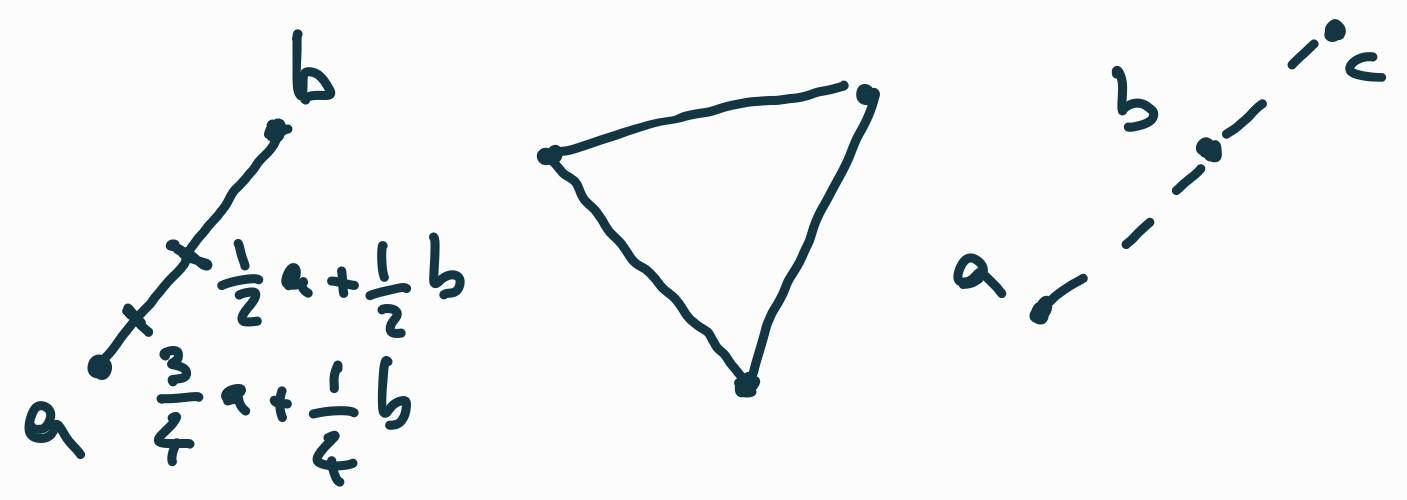
\includegraphics[width=0.5\textwidth]{tempimages/ConvexExamples.jpg}
\end{figure}

\begin{remark}
	In terms of the convex space, all the mixtures between two ensembles correspond to the segment between them; all the mixtures between three ensembles correspond to the triangle formed by the three elements and so on. An ensemble $\ens[a]$ is a component of a different ensemble $\ens[b]$ if the segment connecting $\ens[a]$ and $\ens[b]$ can be extended past $\ens[b]$. If two elements are not a component of each other, then they are the extreme points of the line that connects the two. That is, the segment cannot be extended.
\end{remark}

\begin{figure}[H]
	\centering
	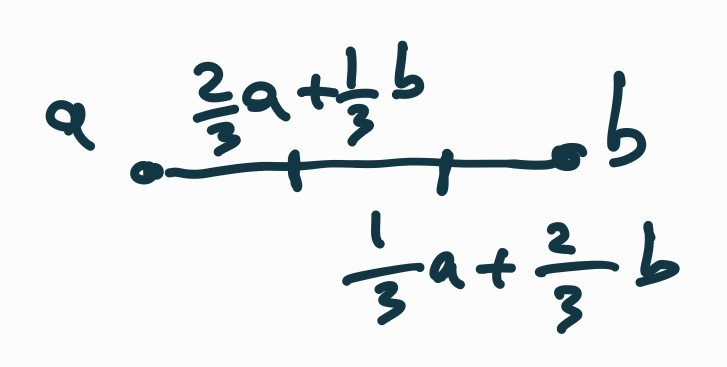
\includegraphics[width=0.4\textwidth]{tempimages/ComponentNotOrder.jpg}
\end{figure}

\begin{remark}
	Note that two ensembles can be components of each other. Consider $\frac{2}{3} \ens[a] + \frac{1}{3} \ens[b]$ and $\frac{1}{3} \ens[a] + \frac{2}{3} \ens[b]$. We can write $\frac{2}{3} \ens[a] + \frac{1}{3} \ens[b] = \frac{1}{2}\left(\frac{1}{3} \ens[a] + \frac{2}{3} \ens[b]\right) + \frac{1}{2} \ens[a]$ and $\frac{1}{3} \ens[a] + \frac{2}{3} \ens[b] = \frac{1}{2}\left(\frac{2}{3} \ens[a] + \frac{1}{3} \ens[b]\right) + \frac{1}{2} \ens[b]$ (they are both midpoints along each other). Therefore a component is not necessarily ``smaller'' or ``better defined'' than the mixture. Mathematically, ``being a component of'' is not a partial order. It is reflexive and transitive, but it is not antisymmetric. In practical terms, we need something else to tell us whether we are, for example, taking a limit with components that become ``smaller and smaller.''
\end{remark}

\begin{defn}
	Let $\Ens$ be an ensemble space and $\ens[a], \ens[b] \in \Ens$. We say that they \textbf{have a common component} if we can find $\ens[c] \in \Ens$, the common component, such that $\ens[a] = p_1 \ens[c] + \bar{p}_1 \ens_1$ and $\ens[b] = p_2 \ens[c] + \bar{p}_2 \ens_2$ for some $\ens_1, \ens_2 \in \Ens$ and $p_1, p_2 \in (0,1]$. Otherwise, we say they \textbf{have no common component}, or are \textbf{separate}, noted $\ens[a] \separate \ens[b]$. Two ensembles have a common component in $A \subseteq \Ens$ if the common component can be found in $A$, and are separate in $A$ if there is none. Two sets of ensembles $A, B \subseteq \Ens$ are separate if all the elements of one are separate from all the elements of the other. That is, $A \separate B$ if $\ens[a] \separate \ens[b]$ for all $\ens[a] \in A$ and $\ens[b] \in B$.
\end{defn}

\begin{figure}[H]
	\centering
	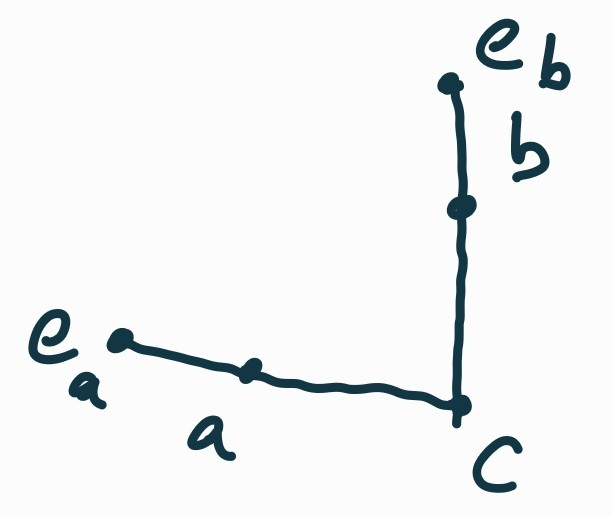
\includegraphics[width=0.3\textwidth]{tempimages/CommonComponent.jpg}
\end{figure}

\begin{remark}
	If two ensembles $\ens[a]$ and $\ens[b]$ have a common component $\ens[c]$, then the ensemble space contains a triangle where $\ens[c]$ is a vertex and $\ens[a]$ and $\ens[b]$ are points on the sides that connect to $\ens[c]$.
\end{remark}

\begin{coro}
	The previous definitions obey the following:
	\begin{enumerate}
		\item every ensemble is a component of itself
		\item if $\ens[a]$ is a component of $\ens[b]$, then $\ens[a]$ and $\ens[b]$ have a common component and therefore they are not separate
		\item separateness is an irreflexive symmetric relation
	\end{enumerate}
\end{coro}

\begin{proof}
	1. Since by idempotence $\ens = p \ens + \bar{p} \ens$ for any $p$, then every ensemble is a mixture of itself, and therefore it is a component of itself.
	
	2. By idempotence, we can write $\ens[a] = p_1 \ens[a] + \bar{p}_1 \ens[a]$ for some $p_1 \in (0,1]$. Since $\ens[a]$ is a component of $\ens[b]$, we can write $\ens[b] = p_2 \ens[a] + \bar{p}_2 \ens[e]_2$ for some $p_2 \in (0, 1]$ and $\ens[c] \in \Ens$. Therefore $\ens[a]$ and $\ens[b]$ have $\ens[a]$ as a common component.
	
	3. Since every ensemble is a component of itself, every ensemble has a common component with itself and therefore is not separate from itself. This proves that separateness is irreflexive. The definition of common component is symmetric and therefore so is separateness.
\end{proof}
\end{mathSection}

Since separateness is defined on top of mixing, it has an important relationship with mixtures: if an ensemble is separate from a mixture of two elements, it is separate from both elements and all their mixtures.

\begin{mathSection}
\begin{prop}[Separateness extends to all mixtures]\label{pm_es_separateExtendsMixtures}
	Let $\ens,\ens_1,\ens_2 \in \Ens$. If $\ens$ has no common component with a mixture of $\ens_1$ and $\ens_2$ then it has no common component with any mixture of $\ens_1$ and $\ens_2$ and with either $\ens_1$ or $\ens_2$. That is, if $\ens \separate p \ens_1 + \bar{p} \ens_2$ for some $p \in (0, 1)$ then $\ens \separate p \ens_1 + \bar{p} \ens_2$ for all $p \in [0, 1]$.
\end{prop}

\begin{figure}[H]
	\centering
	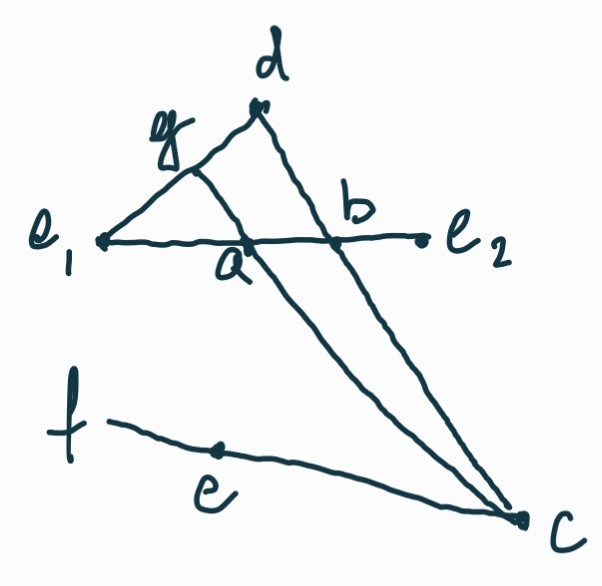
\includegraphics[width=0.3\textwidth]{tempimages/DistinctAndMixture.jpg}
\end{figure}

\begin{proof}
	Let $\ens \separate \ens[a] = p \ens_1 + \bar{p} \ens_2$ for some $p \in (0, 1)$. Let $\ens[b] = \alpha \ens_1 + \bar{\alpha} \ens_2$ with $0 \leq \alpha < p$. Suppose $\ens[b]$ is not separate from $\ens$. Then we can find $\ens[c] \in \Ens$ such that $\ens[b] = \beta \ens[c] + \bar{\beta} \ens[d]$ and $\ens = \gamma \ens[c] + \bar{\gamma} \ens[f]$ for some $\ens[d], \ens[f] \in \Ens$ and $\beta, \gamma \in (0, 1)$.
	
	Setting $\epsilon = \frac{p - \alpha}{\bar{\alpha}}$ and $\lambda = \bar{\epsilon} \beta$ we have:
	\begin{align*}
		\ens[a] &= p \ens_1 + \bar{p} \ens_2 = \left(p - \frac{\bar{p}}{\bar{\alpha}} \alpha \right) \ens_1 + \frac{\bar{p}}{\bar{\alpha}} \alpha \ens_1 + \frac{\bar{p}}{\bar{\alpha}} \bar{\alpha}\ens_2 \\
		&= \left(\frac{p\bar{\alpha} - \bar{p}\alpha}{\bar{\alpha}} \right) \ens_1 + \frac{\bar{p}}{\bar{\alpha}} (\alpha \ens_1 + \bar{\alpha} \ens_2) = \left(\frac{p - p\alpha - \alpha + p \alpha}{\bar{\alpha}} \right) \ens_1 + \frac{1 - p + \alpha - \alpha}{\bar{\alpha}} (\alpha \ens_1 + \bar{\alpha} \ens_2) \\
		&= \frac{p - \alpha}{\bar{\alpha}}  \ens_1 + \left( 1 - \frac{p - \alpha}{\bar{\alpha}}\right) (\alpha \ens_1 + \bar{\alpha} \ens_2) = \epsilon \ens_1 + \bar{\epsilon} (\alpha \ens_1 + \bar{\alpha} \ens_2) = \epsilon \ens_1 + \bar{\epsilon} \ens[b] \\
		&= \epsilon \ens_1 + \bar{\epsilon} ( \beta \ens[c] + \bar{\beta} \ens[d] ) = \bar{\epsilon} \beta \ens[c] + \epsilon \ens_1 + \bar{\epsilon} \bar{\beta} \ens[d] = \lambda \ens[c] + \bar{\lambda} \ens[g]
	\end{align*}
	where $\ens[g] = \frac{1}{\bar{\lambda}}\left( \epsilon \ens_1 + \bar{\epsilon} \bar{\beta} \ens[d] \right)$. This means $\ens[a]$ and $\ens$ have a common component, which is a contradiction. Therefore $\ens \separate \alpha \ens_1 + \bar{\alpha} \ens_2$ for all $\alpha \in [0, p]$.
	
	We can repeat the argument switching $\ens_1$ with $\ens_2$ and find $\ens \separate \alpha \ens_1 + \bar{\alpha} \ens_2$ for all $\alpha \in [0, 1]$.
\end{proof}

\begin{figure}[H]
	\centering
	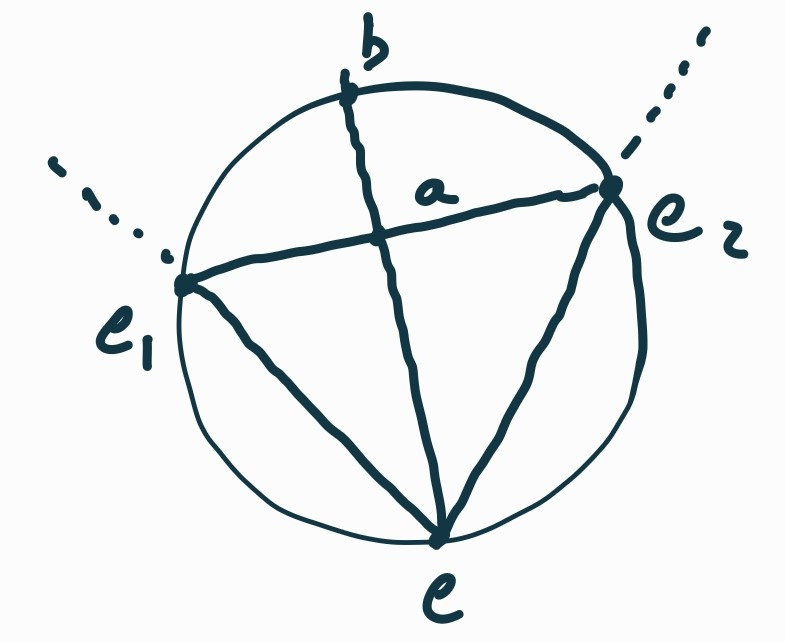
\includegraphics[width=0.3\textwidth]{tempimages/MixturesDoNotPreserveSeparateness.jpg}
\end{figure}

\begin{remark}
	Note that the property does not work the other way around, in the sense that $\ens \separate \ens_1$ and $\ens \separate \ens_2$ does not imply $\ens \separate \alpha \ens_1 + \bar{\alpha} \ens_2$ for all $\alpha \in [0, 1]$. We can find a counterexample in quantum mechanics. Suppose that $\ens$, $\ens_1$ and $\ens_2$ are three pure states within the same two-dimensional subspace. These will be points on the surface of a Bloch ball, which will identify a circle. Since they are pure states, they will be all separate. However, if we take a mixture $\ens[a]$ of $\ens_1$ and $\ens_2$, this can also be written as a mixture of $\ens$ and some $\ens[b]$. Since $\ens$ is a component of $\ens[a]$, they are not separate.
\end{remark}
\end{mathSection}

\subsection{Convex subsets and convex hull}

In many cases, we will need to discuss the set of all possible mixtures of a given set of ensembles. Mathematically, this is the convex closure meaning that we take all possible convex combinations of the given ensembles. Additionally, since the mixture is only a finite operation, we will use the topology to reach all possible limits, all possible infinite mixtures. The topology, in fact, is what defines the limits and will tell us whether a particular infinite convex combination corresponds to a valid mixture or not.

\begin{mathSection}
\begin{defn}
	Let $\Ens$ be an ensemble space. We say $A \subseteq \Ens$ is a \textbf{convex subset} of $\Ens$ if it contains all possible mixtures, including infinite ones, of its elements. Formally, it is a topologically closed set that is also closed under convex combinations. If we want to stress that we are closing only under finite mixing, we say that $A$ is closed under finite convex combination.
\end{defn}

\begin{prop}
	The set $\mathfrak{Conv}_{\Ens}$ of all convex subsets of $\Ens$ ordered by set inclusion is a topped $\bigcap$-structure and therefore is also a complete lattice.
\end{prop}

\begin{proof}
	Let $\mathfrak{Conv}_{\Ens}$ be the set of all convex subsets of $\Ens$ ordered by set inclusion. The empty set $\emptyset \subset \Ens$ is a convex set. The whole space $\Ens \subseteq \Ens$ is also a convex set. Then $\mathfrak{Conv}_{\Ens}$ is therefore a bounded ordered set.
	
	Let $A, B \in \mathfrak{Conv}_{\Ens}$ be two convex subsets. Consider $A \cap B$. Any mixture of elements in $A \cap B$ is both a mixture of elements in $A$ and a mixture of elements in $B$. Therefore any mixture of elements of $A \cap B$ is both an element of $A$ and an element of $B$. This means it is also an element of $A \cap B$, which is therefore a convex set.
	
	The previous argument generalizes to a family of convex subsets $\{A_i\}_{i \in I} \subseteq \mathfrak{Conv}_{\Ens}$. That is, an ensemble is a mixture of elements of $\bigcap_{i \in I} A_i$ if and only if is a mixture of elements of $A_i$ for every $i$. Moreover, the intersection of infinitely many closed sets is still closed. Therefore $\bigcap_{i \in I} A_i \in \mathfrak{Conv}_{\Ens}$ and $\mathfrak{Conv}_{\Ens}$ is an $\bigcap$-structure. This also means that it is a complete lattice. (TODO: find a link to the theorem)
\end{proof}

\begin{defn}
	Let $A \subseteq \Ens$ be a subset of an ensemble space. The \textbf{convex hull} of $A$, noted $\hull(A)$ is the set of all possible mixtures that can be constructed with elements contained in $A$, including infinite ones. Formally, it is the topological closure of the closure of $A$ under convex combination. That is, it is the smallest convex subset that contains $A$.
\end{defn}

\begin{coro}\label{pm_es_hullProp}
	The convex hull has the following properties
	\begin{enumerate}
		\item $A \subseteq \hull(A)$
		\item $A \subseteq B \implies \hull(A) \subseteq \hull(B)$
		\item $\hull(\hull(A)) = \hull(A)$
	\end{enumerate}
	and is therefore a closure operation
\end{coro}

\begin{proof}
	1. Every element of $A$ is trivially a mixture of elements of $A$. Therefore $A \subseteq \hull(A)$.
	
	2. Let $\ens \in \hull(A)$. Then it is a mixture of some elements of $A$. Since $A \subseteq B$, then $\ens$ is also the mixture of some elements of $B$ and therefore $\ens \in \hull(B)$.
	
	3. Since $\hull(\hull(A))$ is the smallest convex subset that contains $\hull(A)$, and since $\hull(A)$ is a convex subset, then $\hull(\hull(A))$ must be $\hull(A)$ since no smaller set can contain all elements of $\hull(A)$.
\end{proof}

\begin{coro}
	A subset $A \subseteq \Ens$ is convex if and only if it is its own convex hull.
\end{coro}

\begin{proof}
	Let $A \subseteq \Ens$ be a convex subset. By \ref{pm_es_hullProp} we have $A \subseteq \hull(A)$. By definition of convex set, we have $\hull(A) \subseteq A$. Therefore $A = \hull(A)$. Conversely, let $A \subseteq \Ens$ be a set of ensembles not necessarily convex. By definition, $\hull(A)$ is closed under mixture and is therefore a convex subset.
\end{proof}

\begin{prop}
	The hull is continuous from above. That is, $\hull(\lim\limits_{i \to \infty} A_i) = \lim\limits_{i \to \infty} \hull(A_i)$ for any decreasing sequence $A_i \subseteq \Ens$.
\end{prop}

\begin{proof}
	Since $A_i$ is a decreasing sequence, $\lim\limits_{i \to \infty} A_i = \bigcap_i A_i$. Also, since $A_{i+1} \subseteq A_i$, then $\hull(A_{i+1}) \subseteq \hull(A_i)$ and therefore $\hull(A_i)$ is a decreasing sequence. This also means $\lim\limits_{i \to \infty} \hull(A_i) = \bigcap_i \hull(A_i)$. Therefore we need to show that $\hull(\bigcap_i A_i) = \bigcap_i \hull(A_i)$.
	
	Since the arbitrary intersection of convex sets is a convex set, $\bigcap_i \hull(A_i)$ is a convex set. Therefore $\bigcap_i \hull(A_i) = \hull(\bigcap_i \hull(A_i))$. Note that a mixture of mixture of elements can always be re-expressed as a mixture of elements. Moreover, an element that is the mixture of $A_i$ for all $i$ can be re-expressed as a mixture of the common elements, since $A_{i+1} \subset A_i$. Therefore $\hull(\bigcap_i \hull(A_i)) = \hull(\bigcap_i A_i)$. This means $\hull(\bigcap_i A_i) = \bigcap_i \hull(A_i)$, which proves the proposition.
\end{proof}

\begin{remark}
	Note that the hull is not necessarily continuous from below. That is, it is not necessarily true that $\hull(\lim\limits_{i \to \infty} A_i) = \lim\limits_{i \to \infty} \hull(A_i)$ for any increasing sequence $A_i \subseteq \Ens$. The limit from below, in fact, would correspond to the infinite union of closed sets, which is not necessarily a closed set. Therefore if we take the closure after the limit, we are going to include the infinite convex combinations that require, for example, an element from each of the $A_i$.
\end{remark}
\end{mathSection}

\begin{conj}
	The topological closure of the finite convex closure is closed under convex combinations.
\end{conj}

\begin{proof}
	Using the axiom of entropy, we know that the ensemble space embeds in a vector space. If we are able to show that it embeds in a topological vector space, then we are taking the closure of a convex subset of a topological vector space. It should be a property that the convex closure should be in the same subspace of the one generated by the convex set. Therefore all limit points would can be generate as limits of elements of the convex set.
\end{proof}

\section{Axiom of entropy}

The third and final property of ensembles is that they have a well-defined entropy. The entropy quantifies the variability of the elements within the ensembles. That is, since an ensemble represents all possible preparations of equivalent systems prepared according to the same procedure, we are asking how much those preparations are different from each other. No matter what the full description of each individual preparation may be, we can assume that their variability has some specific features. It will have to be compatible with experimental verifiability (i.e. the variability must be a continuous function with respect to the topology) and with statistical mixing (i.e. the variability cannot decrease during mixing and it maximally increases when the ensembles do not overlap). The formula for entropy can then be recovered with these very broad physically justified assumptions.

\begin{mathSection}
\begin{axiom}[Axiom of entropy]
	Every element of the ensemble is associated with an \textbf{entropy} which quantifies the variability of the preparations of the ensemble. Formally, an ensemble space $\Ens$ is equipped with a function $S : \Ens \to \mathbb{R}$, defined up to a positive multiplicative constant representing the unit numerical value. The entropy has the following properties:
	\begin{itemize}
		\item \textbf{Continuity}\footnote{Currently, we are imposing that the entropy is continuous. There may be a chance that this requirement is redundant, as strict concavity and the upper variability bound may already impose this. We have found proofs that show that real valued convex/concave functions of real values are continuous. These proofs fail at the extreme points, but the upper variability bound may fix this. Another open question is whether differentiability is also an independent requirement.}
		\item \textbf{Strict concavity}: $S(p\ens[a] + \bar{p} \ens[b]) \geq p S(\ens[a]) + \bar{p} S(\ens[b])$ with the equality holding if and only if $\ens[a] = \ens[b]$
		\item \textbf{Upper variability bound}: there exists a universal function $I(p_1, p_2)$ (i.e. the same for all ensemble spaces) such that $S(p\ens[a] + \bar{p} \ens[b]) \leq I(p, \bar{p}) + p S(\ens[a]) + \bar{p} S(\ens[b])$; if the equality holds, $\ens[a]$ and $\ens[b]$ are \textbf{non-overlapping} or \textbf{orthogonal}, noted $\ens[a] \ortho \ens[b]$
		\item \textbf{Mixtures preserve orthogonality}:\footnote{It is unclear whether ``mixtures preserve orthogonality'' is an independent axiom. Intuitively, the following argument tells us that it is. Take the 2 dimensional simplex (i.e. a triangle) that represents a classical discrete probability space over three elements. Take the standard entropy, which will satisfy ``mixtures preserve orthogonality''. This is because the middle point has entropy $\log 3$. We can imagine redefining the entropy so that it is a little bit lower in the center but it is unchanged on the sides. However, one needs to provide an actual example and show that it satisfies all axioms. It may also be that only one direction is an independent axiom. That is, that orthogonality with the components implies orthogonality with the mixtures. This is what does not hold for separateness.} $\ens[a] \ortho \ens[b]$ and $\ens[a] \ortho \ens[c]$ if and only if $\ens[a] \ortho p \ens[b] + \bar{p} \ens[c]$ for any $p \in (0,1)$
	\end{itemize}
\end{axiom}

\begin{justification}
	The entropy quantifies the variability of the instances of the ensemble. Since the ensemble represents a collection of preparations of equivalent systems, and since each instance will in general be potentially different, it is legitimate to ask how much variability there is among the different instances. We are assuming that the entropy is a quantity (i.e. a linearly ordered property), meaning that it is always meaningful to tell whether one ensemble has more variability than another. If this is the case, the later requirements of continuity and strict concavity will force the entropy to be a real valued quantity. This is because the variability will change under statistical mixtures, and since statistical mixtures are performed with real valued coefficients, the variability will have to be a real valued quantity. Whether it is conceptually possible to have a characterization of variability that is not linearly ordered but still have a meaningful connection with statistical mixing is an open question, therefore we are not able to fully justify entropy's linear ordering at this time. Therefore the linear ordering of the entropy should be considered an assumption. Provided that assumption, we are justified to assume the existence of a real valued function that returns the entropy, a measure of variability of the ensemble.
	
	Since the entropy is a real valued quantity, it will have a corresponding unit. This unit is independent from all other units, and therefore the overall structure of the ensemble space must be independent of this choice. Mathematically, the physical dimension of the unit is not captured, just its numeric value. A change of unit may change the numeric value by a multiplicative constant. Since variability is an ordered quantity, we want the change of units to respect the ordering and therefore it should be a positive multiplicative constant. This justifies that the entropy function is defined up to a positive multiplicative constant.
	
	Note that the additivity of the entropy over independent systems fixes the absolute scale. If $S_{AB} = S_A + S_B$, in fact, one can't rescale all three terms by an additive factor and preserve the relationship.
	
	The variability, in the end, will have physical consequences, and it will therefore be measurable, thus experimentally verifiable: it will have to be a topologically continuous function. Moreover, small changes in the ensemble should produce small changes in the variability, which justifies analytical continuity. We are therefore justified to assume continuity of the entropy.
	
	Suppose we have two ensembles and we perform a statistical mixture. There are going to be three sources of variability: the two ensembles and the random choice at every instance. The total contribution from the original ensembles will be the average variability of the original ensembles. This is increased by the variability introduced by the random choice, which is always a positive contribution. Therefore the final variability cannot be less than the average of the original ensembles. That is, $S(p\ens[a] + \bar{p} \ens[b]) \geq p S(\ens[a]) + \bar{p} S(\ens[b])$. If we are mixing an ensemble with itself, this is equivalent to just choosing from the original ensemble, therefore the variability will not increase. Conversely, if the variability stays the same, it means that the random choice does not increase the variability, and therefore we must be choosing between equivalent ensembles. Therefore we are justified to assume that entropy is strictly concave.
	
	On the other hand, the variability cannot increase arbitrarily during mixture. The maximum variability will be given when the two ensembles are non-overlapping, when an instance of the first ensemble cannot be produced by the second ensemble. That is, a single instance is enough to determine whether we have the first ensemble or the second. In this case, the variability is increased by the variability of the random choice, which must depend only on the mixture coefficient, and not the nature of the ensembles themselves. That is, $S(p\ens[a] + \bar{p} \ens[b]) \leq I(p, \bar{p}) + p S(\ens[a]) + \bar{p} S(\ens[b])$ is the upper variability bound, which is saturated if and only if the $\ens[a]$ and $\ens[b]$ are non-overlapping. The actual function $I$ is left unspecified and, as we show in proposition \ref{pm_es_entropyUnique}, it will correspond to the Shannon entropy as it is the only indicator of variability that will satisfy the axiom of entropy. This justifies the upper variability bound.
	
	Now suppose ensemble $\ens[a]$ is non-overlapping with $\ens[b]$ and $\ens[c]$. That is, an instance of $\ens[a]$ cannot ever be produced by either $\ens[b]$ or $\ens[c]$. Then an instance of $\ens[a]$ cannot be produced by a mixture of $\ens[b]$ and $\ens[c]$, since ultimately a mixture of $\ens[b]$ and $\ens[c]$ will return an instance of one of the two. Therefore $\ens[a]$ is non-overlapping with any mixture of $\ens[b]$ and $\ens[c]$. The argument works in reverse as well: if an instance of $\ens[a]$ cannot be produced by a mixture of $\ens[b]$ and $\ens[c]$, then it cannot be produced by either. This justifies mixtures preserve orthogonality.
\end{justification}
\end{mathSection}

We should now verify that the axiom of entropy is satisfied by the standard cases.

\begin{mathSection}
	\begin{prop}
		Discrete classical ensemble spaces, continuous classical ensemble spaces and quantum ensemble spaces satisfy the axiom of entropy.
	\end{prop}
	
	\begin{proof}
		Let's first look at the classical continuous case. Every ensemble is represented by a distribution $\rho(x)$ with $\int_X \rho(x) d\mu=1$. The entropy is given by $S(\rho) = - \int_X \rho \log \rho d\mu$. This is a continuous function of $\rho$.
		
		\begin{figure}[H]
			\centering
			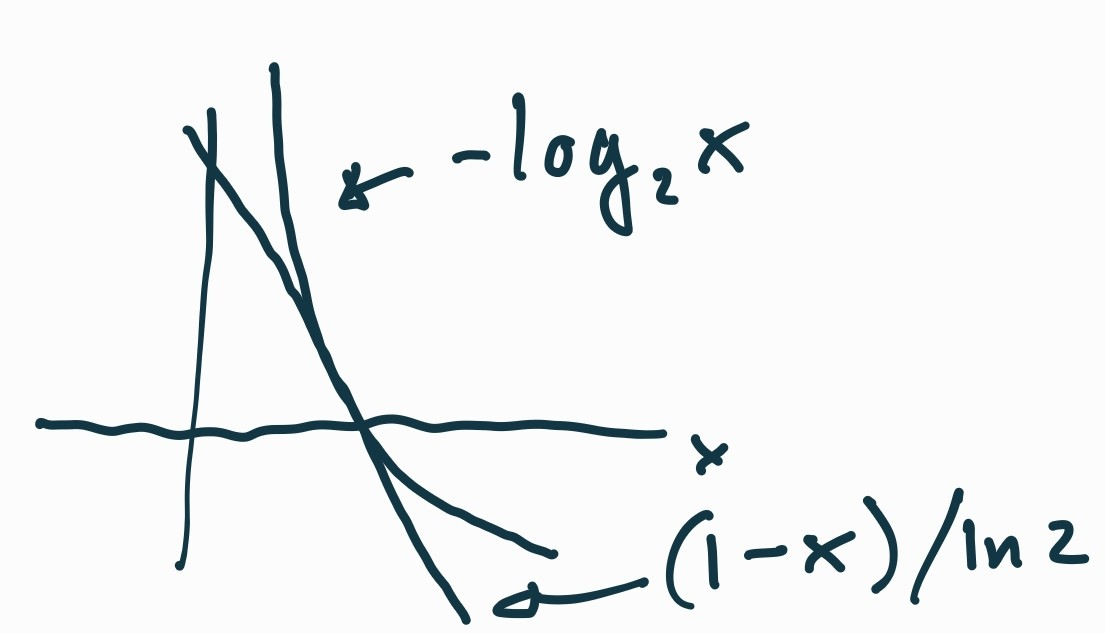
\includegraphics[width=0.5\textwidth]{tempimages/LogBound.jpg}
		\end{figure}
		
		To show strict concavity, note that $- \log x \geq \frac{1-x}{\ln 2}$ with the equality holding if and only if $x=1$. We have
		\begin{equation}
			\begin{aligned}
				S(p\rho_1 + \bar{p}\rho_2) &= - \int_X \left(p\rho_1 + \bar{p}\rho_2\right) \log \left(p\rho_1 + \bar{p}\rho_2\right) d\mu \\
				&= - \int_X p\rho_1 \log \left(p\rho_1 + \bar{p}\rho_2\right) d\mu - \int_X \bar{p}\rho_2 \log \left(p\rho_1 + \bar{p}\rho_2\right) d\mu \\
				&= - \int_X p\rho_1 \log \frac{p\rho_1 + \bar{p}\rho_2}{\rho_1} d\mu - \int_X p\rho_1 \log \rho_1 d\mu \\
				&- \int_X \bar{p}\rho_2 \log \frac{p\rho_1 + \bar{p}\rho_2}{\rho_2} d\mu - \int_X \bar{p}\rho_2 \log \rho_2 d\mu \\
				&\geq \int_X p\rho_1 \frac{1}{\ln 2} \left(1 - \frac{p\rho_1 + \bar{p}\rho_2}{\rho_1} \right)   d\mu - p \int_X \rho_1 \log \rho_1 d\mu \\
				&+ \int_X \bar{p}\rho_2 \frac{1}{\ln 2} \left(1 - \frac{p\rho_1 + \bar{p}\rho_2}{\rho_2} \right)   d\mu - \bar{p} \int_X \rho_2 \log \rho_2 d\mu \\
				&= \frac{p}{\ln 2}\left[ \int_X \rho_1 d\mu - \int_X \left(p\rho_1 + \bar{p}\rho_2\right) d\mu  \right] + p S(\rho_1) \\
				&+ \frac{\bar{p}}{\ln 2}\left[ \int_X \rho_2 d\mu - \int_X \left(p\rho_1 + \bar{p}\rho_2\right) d\mu  \right] + \bar{p} S(\rho_2) \\
				&= \frac{p}{\ln 2}\left[ 1 - 1  \right] + p S(\rho_1) + \frac{\bar{p}}{\ln 2}\left[ 1 - 1 \right] + \bar{p} S(\rho_2) \\
				&= p S(\rho_1) + \bar{p} S(\rho_2) \\
			\end{aligned}
		\end{equation}
		The equality holds if and only if $\frac{p\rho_1 + \bar{p}\rho_2}{\rho_1} = 1$ which is exactly when $\rho_1 = \rho_2$.
		
		
		\begin{figure}[H]
			\centering
			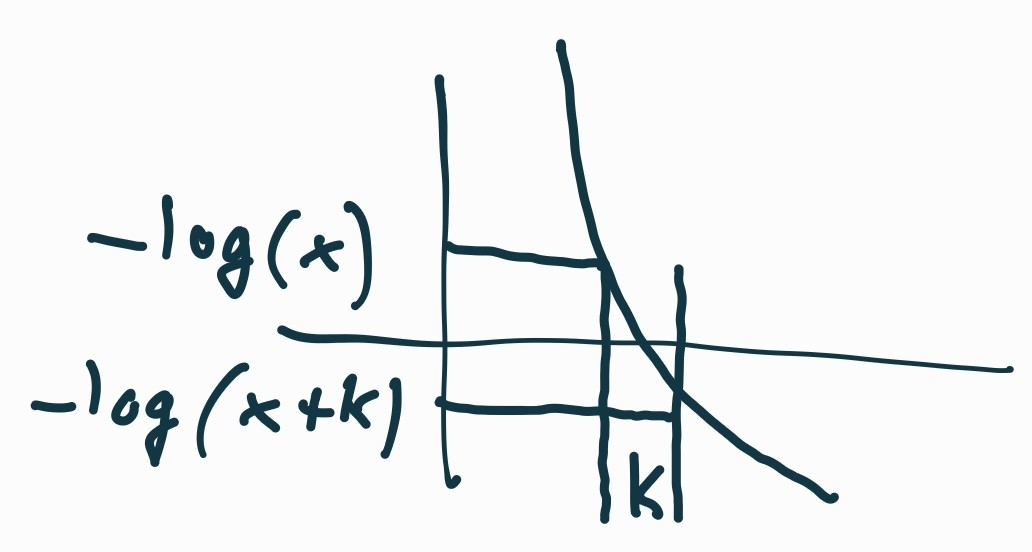
\includegraphics[width=0.5\textwidth]{tempimages/LogMonotone.jpg}
		\end{figure}
		For the upper bound, note that the logarithm is a strictly increasing function, and therefore $- \log(x + k) \leq -\log(x)$ for any $k \geq 0$, with equality holding if and only if $k=0$. We have
		\begin{equation}
			\begin{aligned}
				S(p\rho_1 + \bar{p}\rho_2) &= - \int_X \left(p\rho_1 + \bar{p}\rho_2\right) \log \left(p\rho_1 + \bar{p}\rho_2\right) d\mu \\
				&= - \int_X p\rho_1 \log \left(p\rho_1 + \bar{p}\rho_2\right) d\mu - \int_X \bar{p}\rho_2 \log \left(p\rho_1 + \bar{p}\rho_2\right) d\mu \\
				&\leq  - \int_X p\rho_1 \log p\rho_1 d\mu - \int_X \bar{p}\rho_2 \log \bar{p}\rho_2 d\mu\\
				&=  - \int_X p\rho_1 \log p d\mu - \int_X p\rho_1 \log \rho_1 d\mu - \int_X \bar{p}\rho_2 \log \bar{p} d\mu - \int_X \bar{p}\rho_2 \log \rho_2 d\mu\\
				&=  - p \log p \int_X \rho_1 d\mu - p \int_X \rho_1 \log \rho_1 d\mu - \bar{p} \log \bar{p} \int_X \rho_2 d\mu - \bar{p} \int_X \rho_2 \log \rho_2 d\mu\\
				&=  - p \log p - \bar{p} \log \bar{p} + p S(\rho_1) + \bar{p} S(\rho_2)\\
			\end{aligned}
		\end{equation}
		The equality holds if and only if $\rho_2=0$ wherever $\rho_1\neq0$ and $\rho_1=0$ wherever $\rho_2\neq0$. That is, the equality holds if and only if the two distributions have disjoint support. Therefore orthogonal distributions are exactly distributions with disjoint support.
		
		Suppose $\rho_4$ has disjoint support from $\rho_1 = p \rho_2 + \bar{p} \rho_3$, then it has disjoint support from $\rho_2$ and $\rho_3$ because the support of $\rho_1$ is the union of the supports of $\rho_2$ and $\rho_3$. Conversely, if $\rho_4$ has disjoint support from both $\rho_2$ and $\rho_3$, then $\rho_4$ has disjoint support from $\rho_1$ as well. Therefore mixtures preserve orthogonality.
		
		All these arguments are valid for discrete classical ensemble spaces, changing integrals to sums.
		
		For the quantum case, we haven't found a short proof that does not require defining the KL divergence and the entropy for a joint distribution. The result, however, is generally known and can be found, for example, in \href{https://www.cambridge.org/highereducation/books/quantum-computation-and-quantum-information/01E10196D0A682A6AEFFEA52D53BE9AE}{Nielsen-Chuang}.
	\end{proof}
\end{mathSection}


\subsection{Uniqueness of entropy of mixing coefficients}

We now prove that the function $I(p,\bar{p})$ must be the Shannon entropy.

\begin{mathSection}
\begin{thrm}[Uniqueness of entropy]\label{pm_es_entropyUnique}
	The entropy of the coefficients $I(p,\bar{p})$ is the Shannon entropy. That is, $I(p,\bar{p}) = - \kappa \left(p \log p + \bar{p} \log \bar{p}\right)$ where $\kappa>0$ is the arbitrary multiplicative constant for the entropy. For a mixture of arbitrarily many elements, $I(\{p_i\}) = - \kappa \sum_i p_i \log p_i$.
\end{thrm}

\begin{proof}
	Since the upper entropy bound has to be the same for all spaces, let us assume that $\Ens$ is such that it contains countably many orthogonal ensembles $\{\ens_l\}_{l=1}^{\infty}$. Since mixtures preserve orthogonality, for any convex combinations $\sum_i p_i \ens[a]_i$ of finitely many $\{\ens[a]_i\}_{i=1}^{n} \subset \{\ens_l\}_{l=1}^{\infty}$,  we have $S(\sum_i p_i \ens[a]_i ) = I_n(p_1, p_2, \dots, p_n) + \sum_i p_i S(\ens[a]_i)$ where $I_n : \mathbb{R}^n \to \mathbb{R}$ is a function of the coefficients only. Note that, given commutativity, the order of the $p_i$ does not matter and, since the coefficients can be zero, we must have $I_n(p_1, p_2, \dots, p_n) = I_{n+1}(p_1, p_2, \dots, p_n, 0)$. Therefore we can think of $I$ as a function of the coefficients and write $I(\{p_i\}_{i=1}^{n})$.
	
	We now show that $I\left(\left\{\frac{1}{n}\right\}_{i=1}^{n}\right) = \kappa \log n$ with $\kappa > 0$. That is, the maximum increase of entropy for a uniform distribution is proportional to the logarithm of the number of cases. Pick two positive integers $n, m \in \mathbb{Z}^+$. Pick $nm$ elements $\ens[a]_{jk} \in \{e_l\}_{l=1}^{\infty}$ where $1\leq j \leq n$ and $1 \leq  k \leq m$. We have:
	\begin{equation}
		\begin{aligned}
			S\left(\sum_{j=1}^{n}\sum_{k=1}^{m} \frac{1}{n}\frac{1}{m} \ens[a]_{jk}\right) &= I\left(\left\{ \frac{1}{n}\frac{1}{m}\right\}_{i=1}^{nm}\right) + \sum_{j=1}^{n}\sum_{k=1}^{m} \frac{1}{n}\frac{1}{m} S\left(\ens[a]_{jk}\right) \\
			= S\left(\sum_{j=1}^{n} \frac{1}{n} \sum_{k=1}^{m} \frac{1}{m} \ens[a]_{jk}\right)  &=I\left(\left\{ \frac{1}{n}\right\}_{i=1}^{n}\right) + \sum_{j=1}^{n} \frac{1}{n} S\left(\sum_{k=1}^{m}\frac{1}{m}\ens[a]_{jk}\right) \\
			&=I\left(\left\{ \frac{1}{n}\right\}_{i=1}^{n}\right) + \sum_{j=1}^{n} \frac{1}{n}\left(I\left(\left\{ \frac{1}{m}\right\}_{i=1}^{m}\right) +  \sum_{k=1}^{m}\frac{1}{m}S\left(\ens[a]_{jk}\right)\right) \\
			&=I\left(\left\{ \frac{1}{n}\right\}_{i=1}^{n}\right) + I\left(\left\{ \frac{1}{m}\right\}_{i=1}^{m}\right) + \sum_{j=1}^{n} \sum_{k=1}^{m}\frac{1}{n}\frac{1}{m}S\left(\ens[a]_{jk}\right).
		\end{aligned}
	\end{equation}
	Therefore
	\begin{equation}
		\begin{aligned}
			I\left(\left\{ \frac{1}{nm}\right\}_{i=1}^{nm}\right) &=I\left(\left\{ \frac{1}{n}\right\}_{i=1}^{n}\right) + I\left(\left\{ \frac{1}{m}\right\}_{i=1}^{m}\right).
		\end{aligned}
	\end{equation}
	Note that $f(n) = I\left(\left\{ \frac{1}{n}\right\}_{i=1}^{n}\right)$ is a function of $n$ only, such that $f(nm) = f(n) + f(m)$. Since $f$ is continuous, we have $f(n) = \kappa \log n$. Since the entropy is strictly concave, $\kappa$ must be positive. Therefore
	\begin{equation}
		I\left(\left\{ \frac{1}{n}\right\}_{i=1}^{n}\right) = \kappa \log n
	\end{equation}
	for some $\kappa>0$.
	
	We now show that if the coefficients $p_i$ are rationals, $I_n\left(\left\{ p_i\right\}_{i=1}^{n}\right) = - \kappa \sum_{i=1}^{n} p_i \log p_i$. Let $\{p_i\}_{i=1}^{n}$ be rational coefficients for a convex combination. We can write them as $p_i = \frac{m_i}{m}$ where $\{m_i\}, m \in \mathbb{Z}^+$ and $m$ is the least common denominator. Since $p_i$ are the coefficients of a convex combination, we must have $\sum_{i=1}^{n} m_i = m$. Since $m_i$ is a positive integer, we can write $m_i = \sum_{j=1}^{m_i} 1$. We now take $m$ orthogonal ensembles $\ens[a]_{ij}$ where $1 \leq i \leq n$ and $1 \leq j \leq m_i$. We have
	\begin{equation}
		\begin{aligned}
			S\left(\sum_{i=1}^{n}\sum_{j=1}^{m_i} \frac{1}{m} \ens[a]_{ij}\right) &= I\left(\left\{ \frac{1}{m}\right\}_{i=1}^{m}\right) + \sum_{i=1}^{n}\sum_{j=1}^{m_i} \frac{1}{m} S\left(\ens[a]_{ij}\right) \\
			&= \kappa \log m + \sum_{i=1}^{n}\sum_{j=1}^{m_i} \frac{1}{m} S\left(\ens[a]_{ij}\right) \\
		\end{aligned}
	\end{equation}
	\begin{equation}
		\begin{aligned}
			= S\left(\sum_{i=1}^{n} \frac{m_i}{m} \sum_{j=1}^{m_i} \frac{1}{m_i} \ens[a]_{ij}\right)  &=I\left(\left\{ \frac{m_i}{m}\right\}_{i=1}^{n}\right) + \sum_{i=1}^{n} \frac{m_i}{m}  S\left(\sum_{j=1}^{m_i} \frac{1}{m_i} \ens[a]_{ij}\right) \\
			&=I\left(\left\{ p_i\right\}_{i=1}^{n}\right) + \sum_{i=1}^{n} \frac{m_i}{m}\left(I\left(\left\{ \frac{1}{m_i}\right\}_{i=1}^{m_i}\right) + \sum_{j=1}^{m_i} \frac{1}{m_i} S\left(\ens[a]_{ij}\right)\right) \\
			&=I\left(\left\{ p_i\right\}_{i=1}^{n}\right) + \sum_{i=1}^{n} \frac{m_i}{m} I\left(\left\{ \frac{1}{m_i}\right\}_{i=1}^{m_i}\right) + \sum_{i=1}^{n} \frac{m_i}{m} \sum_{j=1}^{m_i} \frac{1}{m_i}S\left(\ens[a]_{ij}\right) \\
			&=I\left(\left\{ p_i\right\}_{i=1}^{n}\right) + \sum_{i=1}^{n} p_i \kappa \log m_i + \sum_{i=1}^{n}  \sum_{j=1}^{m_i} \frac{1}{m} S\left(\ens[a]_{ij}\right).
		\end{aligned}
	\end{equation}
	Therefore
	\begin{equation}
		\begin{aligned}
			\kappa \log m &= I\left(\left\{ p_i\right\}_{i=1}^{n}\right) + \sum_{i=1}^{n} p_i \kappa \log m_i \\
			I\left(\left\{ p_i\right\}_{i=1}^{n}\right) &= \kappa \log m - \sum_{i=1}^{n} p_i \kappa \log m_i = \sum_{i=1}^{n} p_i \kappa \log m - \sum_{i=1}^{n} p_i \kappa \log m_i \\
			&= - \sum_{i=1}^{n} p_i \kappa \log \frac{m_i}{m} = - \kappa \sum_{i=1}^{n} p_i \log p_i.
		\end{aligned}
	\end{equation}
	
	Lastly, let $\{p_i\}_{i=1}^{n}$ be coefficients for a convex combination, not necessarily rational. Since $I$ is continuous and $p_i$ can be approximated with rational values to an arbitrary level of precision, we will have $I\left(\left\{ p_i\right\}_{i=1}^{n}\right) = - \kappa \sum_{i=1}^{n} p_i \log p_i$. In the case of $n=2$, we have $I(p_1, p_2) = - \kappa p_1 \log p_1 - \kappa p_2 \log p_2$.	
\end{proof}

\begin{coro}
	The unit for the entropy is determined (up to the physical dimension) by the maximum of the entropy of the coefficients $I\left(\frac{1}{2}, \frac{1}{2}\right)$. If the entropy is measured in bits, then $I\left(\frac{1}{2}, \frac{1}{2}\right) = 1$.
\end{coro}

\begin{proof}
	A rescaling of the entropy will also rescale the entropy of the coefficients. Therefore setting the value of the maximum of $I$ will set the arbitrary multiplicative factor. If $I\left(\frac{1}{2}, \frac{1}{2}\right) = 1$, then $\kappa$ is equal to one and the logarithm is base two, which corresponds to the entropy measured in bits. Note that this does not fix the physical dimensions of the entropy, only the numerical value.
\end{proof}
\end{mathSection}

\subsection{Separateness and orthogonality}

Separateness and orthogonality are tightly related to each other. First of all, orthogonality implies separateness and is therefore a stronger property. Moreover, orthogonality is an irreflexive symmetric relation, like separateness.

\begin{mathSection}
\begin{prop}
	Orthogonality satisfies the following properties:
	\begin{enumerate}
		\item irreflexivity: $\ens[a] \northo \ens[a]$
		\item symmetry: $\ens[a] \ortho \ens[b]$ if and only if $\ens[b] \ortho \ens[a]$
		\item components are not orthogonal: if $\ens[b]$ is a component of $\ens[a]$ then $\ens[a] \northo \ens[b]$
		\item orthogonality implies separateness: if $\ens[a] \ortho \ens[b]$ then $\ens[a] \separate \ens[b]$.
	\end{enumerate}
\end{prop}

\begin{proof}
	For 1, let $\ens[a] \in \Ens$. We have $S(p\ens[a] + \bar{p}\ens[a]) = S(\ens[a]) < I(p,\bar{p}) + p S(\ens[a]) + \bar{p} S(\ens[a])$. Therefore $\ens[a]$ is not orthogonal to itself as it does not saturate the upper bound.
	
	For 2, note that the upper entropy bound is symmetric in $\ens[a]$ and $\ens[b]$.
	
	For 3, let $\ens[a] = p \ens[b] + \bar{p} \ens[c]$. Since mixtures preserve orthogonality, $\ens[b] \ortho \ens[a]$ if and only if $\ens[b] \ortho \ens[b]$ and $\ens[b] \ortho \ens[c]$. But $\ens[b]$ is not orthogonal to itself, therefore $\ens[a]$ and $\ens[b]$ are not orthogonal.
	
	For 4, we demonstrate the contrapositive: that ensembles that are not separate are not orthogonal. Let $\ens[a], \ens[b] \in \Ens$ have a common component. That is, $\ens[a] = p \ens[c] + \bar{p} \ens[d]$ and $\ens[b] = \lambda \ens[c] + \bar{\lambda} \ens[e]$. Since mixtures preserve orthogonality, $\ens[a] \ortho \ens[b]$ if and only if $\ens[a] \ortho \ens[c]$ and $\ens[a] \ortho \ens[e]$. But $\ens[c]$ is a component of $\ens[a]$, therefore they are not orthogonal. Therefore two ensembles that have a common component are not orthogonal. This means that if two ensembles are orthogonal they cannot have a common component and are therefore separate.
\end{proof}

As we did for separateness, we extend the notion of orthogonality to sets of ensembles.

\begin{defn}
	Two sets of ensembles are orthogonal if all the elements of one are orthogonal to all the elements of the other. That is, $A \ortho B$ with $A, B \subseteq \Ens$ if $\ens[a] \ortho \ens[b]$ for all $\ens[a] \in A$ and $\ens[b] \in B$. 
\end{defn}

\begin{prop}
	Let $A, B \subseteq \Ens$ be two sets of ensembles such that $A \ortho B$. Then the following are true:
	\begin{enumerate}
		\item the two sets are separate: $A \separate B$
		\item their hulls are orthogonal: $\hull(A) \ortho \hull(B)$
	\end{enumerate}
\end{prop}

\begin{proof}
	For 1, by definition $\ens[a] \ortho \ens[b]$ for all $\ens[a] \in A$ and $\ens[b] \in B$. Since orthogonality implies separateness, we also have $\ens[a] \separate \ens[b]$.
	
	For 2, since mixtures preserve orthogonality, every mixture of $A$ is orthogonal to every mixture of $B$. To show that this extends to the closure, let $\ens[a]_i \in A$ and $\ens[b]_j \in B$ be two sequences of finite mixtures that converge in $A$ and $B$ respectively. Consider $f(p,\ens[a]_i, \ens[b]_j) = S(p \ens[a]_i + \bar{p} \ens[b]_j) - p S(\ens[a]_i) - \bar{p} S(\ens[b]_j)$. Since all mixtures are orthogonal, $f(p,\ens[a]_i, \ens[b]_j) = I(p,\bar{p})$. Note that $f$ is a continuous function, therefore the limits will also converge to $I(p,\bar{p})$. This means that every element in the hull of $A$ is orthogonal to every element in the hull of $B$.
\end{proof}
\end{mathSection}

\section{Entropic constraints on the space}

The axiom of entropy not only constrains the functional form of the entropy, but it also constrains the type of space we can have. Additionally, it rules out some spaces that would seem physically pathological.

The entropic structure, in general, will constrain both the topological structure, making it metrizable, and the convex structure, making it embeddable in a vector space. The entropy is also responsible for all the geometric structure of the ensemble space.


\subsection{Vector space embedding}

The axiom of mixture does not constrain the convex set to be a subset of a vector space. The axiom of entropy, however, does. To be specific, it is the first three properties of the entropy that constrain the space.

\begin{mathSection}
\begin{prop}
	A convex space $X$ embeds into a vector space if and only if it is \textbf{cancellative}, that is $p \ens[a] + \bar{p} \ens = p \ens[b] + \bar{p} \ens$ for some $p \in (0,1)$ implies $\ens[a] = \ens[b]$.
\end{prop}

\begin{proof}
	Theorem 4 in \href{https://arxiv.org/abs/1105.1270}{this paper} states that a convex space embeds into a real vector space with $c_\lambda(x,y) = \lambda x + \bar{\lambda}y$ if and only if
	$$ c_\lambda(x,y) = c_\lambda(x,z) \; \forall \lambda \in (0,1) \implies y = z.$$ TODO: the proof should be adapted and carried over.
\end{proof}

\begin{thrm}[Vector space embedding]
	Let $\ens[a], \ens[b], \ens \in \Ens$ such that $p\ens[a] + \bar{p} \ens = p \ens[b] + \bar{p} \ens$ for some $p \in (0,1)$. Then $\ens[a] = \ens[b]$. Therefore any ensemble space embeds into a real vector space.
\end{thrm}

\begin{proof}
	Let $\ens[a], \ens[b], \ens \in \Ens$ such that $p_0\ens[a] + \bar{p}_0 \ens = p_0 \ens[b] + \bar{p}_0 \ens$ for some $p_0 \in (0,1)$.
	
	First, we show that $p\ens[a] + \bar{p} \ens = p \ens[b] + \bar{p} \ens$ for all $p \in (0,p_0]$. In that case, since $0 < \frac{p}{p_0} \leq 1$, we have
	\begin{equation}
		\begin{aligned}
			p \ens[a] + \bar{p} \ens &= \frac{p}{p_0} (p_0 \ens[a] + \bar{p}_0 \ens) + \overline{\left(\frac{p}{p_0}\right)} \ens = \frac{p}{p_0} (p_0 \ens[b] + \bar{p}_0 \ens) + \overline{\left(\frac{p}{p_0}\right)} \ens = p \ens[b] + \bar{p} \ens.
		\end{aligned}
	\end{equation}
	
	Now we show that $p\ens[a] + \bar{p} \ens = p \ens[b] + \bar{p} \ens$ for all $p \in (0,1)$. Since we want to be able to expand multiple times, we want to be able to find a $p \in (0,1)$ such that
	\begin{equation}
		p \ens[a] + p \ens[a] + (1-2p) \ens = p \ens[a] + \bar{p} (p_0 \ens[a] + \bar{p}_0 \ens)= p \ens[a] + \bar{p} p_0 \ens[a] + \bar{p} \bar{p}_0 \ens.
	\end{equation}
	The coefficient of the middle term on both sides of the equality, then, has to match. That is, we want $p = \bar{p} p_0$, which means
	\begin{equation}
		\begin{aligned}
			p&=(1-p)p_0=p_0 - p p_0 \\
			p_0 &= p + p p_0 = (1+p_0) p  \\
			p &= \frac{p_0}{1+p_0}
		\end{aligned}
	\end{equation}
	Note that since $p_0 > 0$ we have $p>0$, and since the numerator is always greater than the denominator $p < 1$. We have
	\begin{equation}
		\begin{aligned}
			2p \ens[a] + \overline{2p} \ens &=  p \ens[a] + p \ens[a] + (1-2p) \ens =  p \ens[a] + \bar{p} (p_0 \ens[a] + \bar{p}_0 \ens) = p \ens[a] + \bar{p} (p_0 \ens[b] + \bar{p}_0 \ens) \\
			&= p \ens[a] + p \ens[b] + (1-2p) \ens = p \ens[b] + p \ens[a] + (1-2p) \ens = p \ens[b] + \bar{p} (p_0 \ens[a] + \bar{p}_0 \ens) \\
			&= p \ens[b] + \bar{p} (p_0 \ens[b] + \bar{p}_0 \ens) = p \ens[b] + p \ens[b] + (1-2p) \ens \\
			&= 2p \ens[b] + \overline{2p} \ens
		\end{aligned}
	\end{equation}
	The relationship, then, is valid for $p_1 = 2p$. Note that $p_1 > p_0$. In fact
	\begin{equation}
		\begin{aligned}
			p_1 &= \frac{2p_0}{1+p_0} > p_0  \\
			2 p_0 &> (1+p_0) p_0 = p_0 + p_0^2 \\
			p_0 &> p_0^2 \\
		\end{aligned}
	\end{equation}
	which is true since $p_0 \in (0,1)$. Since now the relationship holds for $p_1 = \frac{2 p_0}{1+p_0} > p_0 $, we can repeat the process again and find that it holds for $p_2 = \frac{2 p_1}{1+p_1} > p_1$ and so on. We thus have a sequence of elements between $0$ and $1$ and we need to determine what is the limit of this sequence. The only two fixed points of the expression $f(x) = \frac{2x}{1+x}$ are $0$ and $1$, with $0$ being a repelling fixed point and $1$ an attracting fixed point. Since we start with an element that is strictly between those values, the sequence will converge to $1$. Therefore, since we can always find a greater mixing coefficient for which the relationship holds, combined with the previous result, $p\ens[a] + \bar{p} \ens = p \ens[b] + \bar{p} \ens$ for all $p \in (0,1)$.
	
	Now we show that if  $p\ens[a] + \bar{p} \ens = p \ens[b] + \bar{p} \ens$ for all $p \in (0,1)$, then we also have $p(\lambda\ens[a] + \bar{\lambda}\ens[b]) + \bar{p} \ens = p\ens[a] + \bar{p} \ens = p \ens[b] + \bar{p} \ens$ for all $\lambda \in [0,1]$. We have
	\begin{equation}
		\begin{aligned}
			p(\lambda\ens[a] + \bar{\lambda}\ens[b]) + \bar{p} \ens &= \lambda(p \ens[a] + \bar{p} \ens) + \bar{\lambda}(p\ens[b] + \bar{p} \ens) = \lambda(p \ens[a] + \bar{p} \ens) + \bar{\lambda}(p\ens[a] + \bar{p} \ens) \\
			&= p\ens[a] + \bar{p} \ens = p\ens[b] + \bar{p} \ens 
		\end{aligned}
	\end{equation}
	
	Lastly, we show that $S(\lambda \ens[a] + \bar{\lambda} \ens[b]) = S(\ens[a]) = S(\ens[b])$ for all $\lambda \in [0,1]$. Using the entropy bounds, with $\lambda \in [0,1]$, we have
	\begin{equation}
		\begin{aligned}
			\lim\limits_{p \to 1} S(p(\lambda\ens[a] + \bar{\lambda}\ens[b]) + \bar{p}\ens) &\leq \lim\limits_{p \to 1} \left[ I(p,\bar{p}) + p S(\lambda\ens[a] + \bar{\lambda}\ens[b]) + \bar{p} S(\ens) \right] = S(\lambda\ens[a] + \bar{\lambda}\ens[b]) \\
			\lim\limits_{p \to 1} S(p(\lambda\ens[a] + \bar{\lambda}\ens[b]) + \bar{p}\ens) &\geq \lim\limits_{p \to 1} \left[ p S(\lambda\ens[a] + \bar{\lambda}\ens[b]) + \bar{p} S(\ens) \right] = S(\lambda\ens[a] + \bar{\lambda}\ens[b])
		\end{aligned}
	\end{equation}
	and therefore
	\begin{equation}
		\begin{aligned}		
			\lim\limits_{p \to 1} S(p(\lambda\ens[a] + \bar{\lambda}\ens[b]) + \bar{p}\ens) &= S(\lambda\ens[a] + \bar{\lambda}\ens[b]).
		\end{aligned}
	\end{equation}
	Using the above property, we also have
	\begin{equation}
		\begin{aligned}
			S(\lambda\ens[a] + \bar{\lambda}\ens[b]) &= \lim\limits_{p \to 1} S(p(\lambda\ens[a] + \bar{\lambda}\ens[b]) + \bar{p}\ens) = \lim\limits_{p \to 1} S(p \ens[a] +\bar{p} \ens) = S(\ens[a]) \\
			&= \lim\limits_{p \to 1} S(p \ens[b] +\bar{p} \ens) = S(\ens[b]) \\
		\end{aligned}
	\end{equation}
	Since $S(\lambda\ens[a] + \bar{\lambda}\ens[b]) = \lambda S(\lambda\ens[a] + \bar{\lambda}\ens[b]) + \bar{\lambda} S(\lambda\ens[a] + \bar{\lambda}\ens[b]) = \lambda S(\ens[a]) + \bar{\lambda} S(\ens[b])$, $\ens[a] = \ens[b]$ by strict concavity.
\end{proof}

\begin{defn}
	An element $\ens \in \Ens$ can be expressed as an \textbf{affine combination} of ensembles $\ens = \sum_{i=1}^{n} p_i \ens_i$, where $\ens_i \in \Ens$, $p_i \in \mathbb{R}$ and $\sum_{i=1}^{n} p_i = 1$, if the linear combination in the vector space returns an element of $\Ens$.
\end{defn}

\begin{remark}
	In the same way that not all infinite convex combinations yield valid ensembles, not all finite or infinite affine combinations yield valid ensembles.
\end{remark}

\begin{conj}\label{pm_es_ensemblesAreTVS}
	An ensemble space embeds continuously in a topological vector space.
\end{conj}

\begin{remark}
	It is still an open question whether the ambient vector space must be a topological vector space. Axioms of ensemble and mixture are not enough to guarantee the topological nature of the vector space. See \href{https://math.stackexchange.com/questions/4921905/cancellative-convex-spaces-and-topological-vector-spaces}{this post}. The issue is that we have no guarantee of continuity on the inverse (i.e. subtraction, multiplication by a negative number). As it is shown later, the entropy provides a pseudo-distance, which allows one to create open balls. Moreover, the entropy induces a metric tensor, which may induce a suitable topology.
\end{remark}

\end{mathSection}

\subsubsection{Self-mixtures}

As an example of a convex space that is non-cancellative, does not embed in a vector space, and therefore is ruled out as an ensemble space, we consider one in which the convex combination of two different elements returns the first. We show that this can be made to satisfy the axioms of ensemble and mixture, and therefore it is really the axiom of entropy that rules it out.

\begin{example}[Self-mixture]
	Let $\Ens = \{\ens[a], \ens[b]\}$ be a set endowed with the convex structure that satisfies identity, idempotence, commutativity and such that $p \ens[a] + \bar{p} \ens[b]$ equals $\ens[a]$ if $p=1$ and $\ens[b]$ otherwise. Identity, idempotence and commutativity are satisfied by construction. For associativity, note that the final result of multiple mixtures is $\ens[a]$ if and only if all elements of the mixtures are $\ens[a]$. The order does not matter, and therefore associativity is satisfied. Therefore such structure satisfies at least the axiom of mixture without the requirement of continuity.
	
	For continuity, we need to look at the inverse image under the mixing operation. Note that $+^{-1}(\emptyset) = \emptyset$ and $+^{-1}(\Ens) = [0,1] \times \Ens \times \Ens$. Since $\emptyset$ and $\Ens$ must be in any topology of $\Ens$, the continuity condition is satisfied for these sets. Next, we have  $+^{-1}(\{\ens[a]\}) = [0,1] \times \{\ens[a]\} \times \{\ens[a]\} \cup [1] \times \{\ens[a]\} \times \{\ens[b]\} \cup [0] \times \{\ens[b]\} \times \{\ens[a]\}$. Note that $[0]$ and $[1]$ are not open sets, therefore $\{\ens[a]\}$ cannot be in the topology of $\Ens$ or mixing would not be continuous. Finally, $+^{-1}(\{\ens[b]\}) = [0,1] \times \{\ens[b]\} \times \{\ens[b]\} \cup [0,1) \times \{\ens[a]\} \times \{\ens[b]\} \cup (0,1] \times \{\ens[b]\} \times \{\ens[a]\} = [0,1) \times \Ens \times \{\ens[b]\} \cup (0,1] \times \{\ens[b]\} \times \Ens$. Since $(0,1]$ and $[0,1)$ are open subsets of $[0,1]$, \{$\ens[b]\}$ can be an open set. Since the topology must be $\textsf{T}_0$, we must include at least $\{\ens[b]\}$ and therefore $\mathsf{T}_{\Ens} = \{\emptyset, \{\ens[b]\}, \{\ens[a], \ens[b]\}\}$ is a $\mathsf{T}_0$ second countable topology for which mixing is continuous. This means that the example satisfies both the axioms of ensemble and of mixture.
\end{example}

It is therefore the entropy that rules out this case. If the entropy of the two ensembles is different, it would jump from $S(\ens[a])$ directly to $S(\ens[b])$ for an infinitesimal mixture which violates the upper bound. If $S(\ens[a])$ equals $S(\ens[b])$, the entropy of the mixture of $\ens[a]$ and $\ens[b]$ is also the same, so the two ensembles cannot possibly be different by strict concavity.

Intuitively, this tells us that we cannot have a mixture of two different elements that happens to be equal to one of the original elements.

\begin{mathSection}
	\begin{coro}
		Let $\ens[a], \ens[b] \in \Ens$ such that $p\ens[a] + \bar{p} \ens[b] = \ens[b]$ for some $p \in (0,1]$. Then $\ens[a] = \ens[b]$. 
	\end{coro}
	
	\begin{proof}
		We have $p\ens[a] + \bar{p} \ens[b] = \ens[b] = p\ens[b] + \bar{p} \ens[b]$ for some $p \in (0,1]$. Therefore $\ens[a] = \ens[b]$.
	\end{proof}
\end{mathSection}

\subsection{Boundedness of lines}

Another constraint that the entropy imposes is that every affine direction is bounded, even if there are no endpoints. That is, if we take two ensembles, these will identify a line that contains all the affine combinations in the vector space. The elements of that line that are also in the ensemble space are contained in a bounded segment of that line.

\begin{figure}[h]
	\centering
	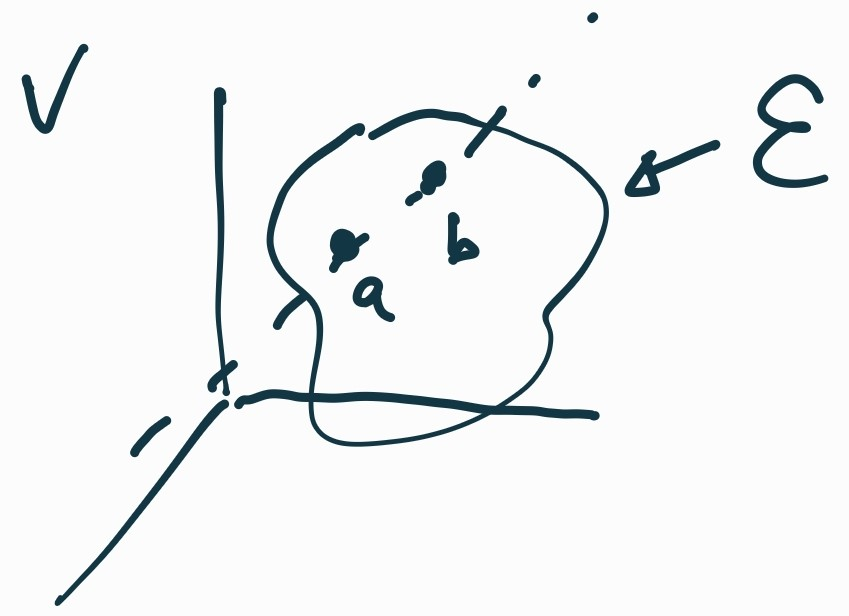
\includegraphics[width=0.4\textwidth]{tempimages/BoundedEnsembleSpace.jpg}
	\caption{$\Ens$ is the ensemble space and $V$ is the embedding vector space. Taking two ensembles, the dashed line represents all the affine combinations. Those that are in the ensemble space are a line, as defined below.}
\end{figure}

\begin{mathSection}
\begin{defn}
	A \textbf{line} $A \subseteq \Ens$ is a convex subset such that for any three elements one can be expressed as a mixture of the other two. That is, for all $\ens_1, \ens_2, \ens_3 \in A$ there exists a permutation $\sigma : \{1,2,3\} \to \{1,2,3\}$ and $p \in [0,1]$ such that $\ens_{\sigma(1)} = p \ens_{\sigma(2)} + \bar{p} \ens_{\sigma(3)}$.
\end{defn}

\begin{prop}
	Given $\ens[a], \ens[b] \in \Ens$, there is only one line that contains them.
\end{prop}

\begin{proof}
	Since an ensemble space embeds into a vector space, given two ensembles there is only one affine line that connects them. A line is the intersection of the affine line with the ensemble space.
\end{proof}

\begin{thrm}[Lines are bounded]
	Let $A \subseteq \Ens$ be a line. Then we can find a bounded interval $V \subseteq \mathbb{R}$ and an invertible function $f : A \to V$ such that $f(p \ens[a] + \bar{p} \ens[b]) = p f(\ens[a]) + \bar{p} f(\ens[b])$ for all $\ens[a], \ens[b] \in A$.
\end{thrm}

\begin{proof}
	Let $A \subseteq \Ens$ be a line. Pick $\ens_0, \ens_1 \in A$. For any $\ens[a] \in A$, we can find an affine expression between $\ens_0$, $\ens_1$ and $\ens[a]$. Rearranging the terms, we can always write $\ens[a] = \bar{x}\ens_0 + x\ens_1$ where $x \in \mathbb{R}$. Note that $x$ uniquely determines $\ens[a]$. Therefore we can define $f(\ens[a]) \mapsto x$, and it will be an invertible function.
	
	We can verify that, given $\ens[a], \ens[b] \in A$, we have
	\begin{equation}
		\begin{aligned}
			f(p\ens[a] + \bar{p} \ens[b]) &= f(p\bar{x}_a \ens_0 + px_a \ens_1 + \bar{p}\bar{x}_b \ens_0 + \bar{p}x_b \ens_1) = f((p\bar{x}_a + \bar{p}\bar{x}_b) \ens_0 + (px_a + \bar{p}x_b) \ens_1) \\
			&= px_a + \bar{p}x_b = pf(\ens[a]) + \bar{p}f(\ens[b]).
		\end{aligned}
	\end{equation}
	
	We are going to show that the image $V=f(A)$ must be a bounded set, or it would eventually violate the entropy bounds. Given a value $x \in V$, there will be an entropy value $S(f^{-1}(x))$ which we can write as a function of the real value $S(x)$. This function will need to satisfy continuity, strict concavity and the upper variability bound.

\begin{figure}[H]
	\centering
	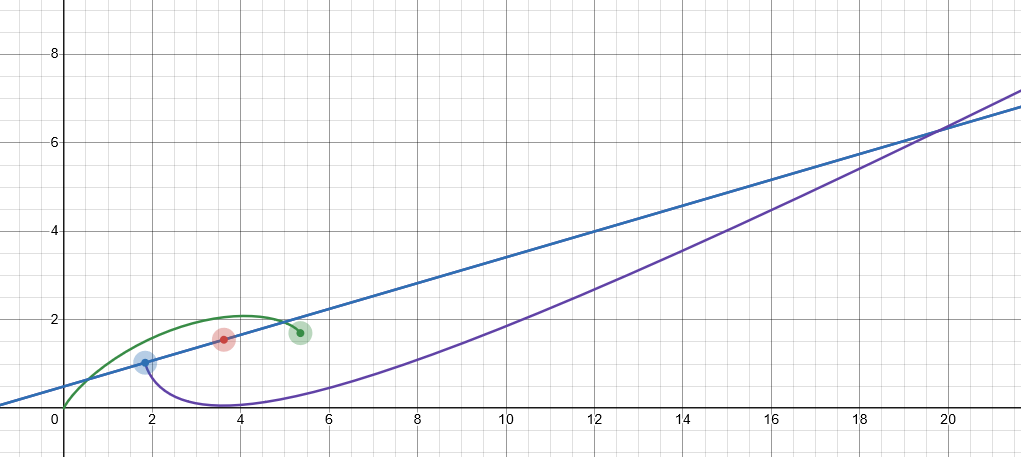
\includegraphics[width=0.7\textwidth]{tempimages/BoundsFromEntropy.png}
	\caption{Visual representation of the bounds. See proof for details.}
\end{figure}
	We are going to show that the function $S(x)$ cannot extend to plus infinity. The same argument can be applied by symmetry for minus infinity. We are going to assume that $S(0) = 0$ without loss of generality. If $S$ is not defined at zero, or if the value is different, we can apply a translation on the argument or on the value, which will not affect the concavity of the function.
	
	Let $0 < a < b \in V$ be two distinct values, with $S(a)$ and $S(b)$ their respective entropies. We are going to show that if we pick a $c > b$ sufficiently large, we are not going to find a value for $S(c)$ that satisfies the bounds. In the picture, we have the three points, $a$ in blue, $b$ in red, $c$ in green. The horizontal axis represent the value, the position of the ensemble along the affine line, while the vertical axis represents the entropy. Consider the points $a$, $b$ and $c$. Since the entropy is strictly concave, $c$ must be placed under the blue line which represents an upper bound on $S(c)$. Now consider $0$, $a$ and $c$. Since $a$ is a mixture of $0$ and $c$, $S(a)$ will need to satisfy the upper bound given by $S(0)$ and $S(c)$. In the diagram, the green line represents the upper bound on $S(a)$ for the specific choice of $c$ and $S(c)$. Since $a$ and $S(a)$ are fixed, this puts a lower bound on $S(c)$, which is represented by the purple curve. That is, the purple curve represents the minimum value we have to assign to $S(c)$ such that $S(a)$ still satisfies the upper bound between $0$ and $c$. As the picture shows, the two bounds meet at some point and cannot both be satisfied.
	
	From strict concavity, noting that $\frac{c-b}{c-a} + \frac{b-a}{c-a} = 1$, we have:
	\begin{equation}
		\begin{aligned}
			S(b) &= S\left(\frac{c-b}{c-a} a + \frac{b-a}{c-a} c\right) > \frac{c-b}{c-a} S(a) + \frac{b-a}{c-a} S(c)\\
			(b-a)S(c) &< (c-a) S(b) - (c-b) S(a) = (c-a) S(b) - (c-a) S(a) + (b-a) S(a) \\
			S(c) &< \frac{S(b) - S(a)}{(b-a)} (c-a) + S(a) \\
		\end{aligned}
	\end{equation}
	
	From the upper bound, noting that $\frac{c-a}{c} + \frac{a}{c} = 1$ and recalling we assumed $S(0) = 0$, we have:
	\begin{equation}
		\begin{aligned}
			S(a) &= S\left(\frac{c-a}{c} 0 + \frac{a}{c} c\right) \leq I\left(\frac{c-a}{c}, \frac{a}{c}\right) + \frac{c-a}{c} S(0) +\frac{a}{c} S(c) \\
			\frac{a}{c} S(c) &\geq S(a) - I\left(\frac{c-a}{c}, \frac{a}{c}\right) \\
			S(c) &\geq \frac{c}{a} \left[ S(a) - I\left(\frac{c-a}{c}, \frac{a}{c}\right) \right]
		\end{aligned}
	\end{equation}
	
	Combining the bounds, we have:
	\begin{equation}
		\begin{aligned}
			\frac{S(b) - S(a)}{(b-a)} (c-a) + S(a) &> \frac{c}{a} \left[ S(a) - I\left(\frac{c-a}{c}, \frac{a}{c}\right) \right] \\
			(c-a) S(b) - (c-a)S(a) + (b-a) S(a) &> \frac{c(b-a)}{a} S(a) - \frac{c(b-a)}{a} I\left(\frac{c-a}{c}, \frac{a}{c}\right) \\
			a (c-a) S(b) - a(c-b) S(a) &> c(b-a)S(a) - c(b-a) I\left(\frac{c-a}{c}, \frac{a}{c}\right) \\
			a (c-a) S(b) + (-ac +ab -bc +ac) S(a) &> - c(b-a) I\left(\frac{c-a}{c}, \frac{a}{c}\right) \\
			a (c-a) S(b) -b (c-a) S(a) &> - c(b-a) I\left(\frac{c-a}{c}, \frac{a}{c}\right) \\
			a  S(b) - b S(a) &> - \frac{c(b-a)}{(c-a)} I\left(\frac{c-a}{c}, \frac{a}{c}\right) \\
		\end{aligned}
	\end{equation}
	
	Since $b > a$, $c > a$ and $I(p,\bar{p}) > 0$ for all $p \in (0,1)$, the right hand side of the inequality is always negative. As $c$ increases, the right hand side will go to zero, since $\lim\limits_{c\to \infty}\frac{c(b-a)}{c-a} = b-a$ and $\lim\limits_{c\to \infty} I\left(\frac{c-a}{c}, \frac{a}{c}\right) = I(1,0) = 0$. The left hand side is a constant. If the constant is positive, the inequality is always satisfied. If it is negative, it will not be satisfied for all $c$.
	
	From strict concavity, noting that $\frac{b-a}{b} + \frac{a}{b} = 1$, we have
	\begin{equation}
		\begin{aligned}
			S(a) &= S\left(\frac{b-a}{b} 0 + \frac{a}{b} b\right) > \frac{b-a}{b} S(0) + \frac{a}{b} S(b) = \frac{a}{b} S(b)\\
			b S(a) &> a S(b)  \\
			0 &> a S(b) - b S(a)\\
		\end{aligned}
	\end{equation}
	This shows that the left hand side of the previous inequality is negative, and therefore the bounds cannot be satisfied over the whole $\mathbb{R}$.
	
	This means that $V = f(A)$ must be bounded and therefore every line is a segment as embedded in the vector space.
\end{proof}

\begin{remark}
	Note that this does not mean that, along each direction, the line is closed in the vector space. That is, it may not include the extreme points. in the convex space. An open bounded interval, in fact, is still a convex space and we would be able to define an entropy on it.
\end{remark}
\end{mathSection}

\section{Entropic geometry}

We now show that the entropy imposes a geometric structure on the ensemble space. The core idea is that, since the entropy is strictly concave, its Hessian is negative definite. The negation is therefore a positive definite, real-valued function of two variations and plays the role of a metric tensor.

\subsection{Mixing entropy as pseudo-distance}

The first observation is that the entropy can be used to define a pseudo-distance. If we mix two ensembles, in fact, the average entropy cannot decrease, and will stay the same if the two components of the mixture are the same ensemble. The increase, then, is zero if the two ensembles are equal, greater than zero if not, with the maximum if they are orthogonal. 

\begin{mathSection}
\begin{defn}
	Given two ensembles $\ens[a], \ens[b] \in \Ens$, the \textbf{mixing entropy}, also called Jensen-Shannon divergence, is the increase in entropy associated to their equal mixture. That is:
	$$MS(\ens[a], \ens[b]) = S\left(\frac{1}{2}\ens[a] + \frac{1}{2} \ens[b]\right) - \left(\frac{1}{2} S(\ens[a]) + \frac{1}{2} S(\ens[b])\right).$$
\end{defn}

\begin{prop}
	The mixing entropy $MS(\ens[a], \ens[b])$ satisfies the following:
	\begin{enumerate}
		\item \textbf{non-negativity}: $MS(\ens[a], \ens[b]) \geq 0$
		\item \textbf{identity of indiscernibles}: $MS(\ens[a], \ens[b]) = 0 \iff \ens[a]=\ens[b]$
		\item \textbf{unit boundedness}: $MS(\ens[a], \ens[b]) \leq 1$
		\item \textbf{maximality of orthogonals}: $MS(\ens[a], \ens[b]) = 1 \iff \ens[a] \ortho \ens[b]$
		\item \textbf{symmetry}: $MS(\ens[a], \ens[b]) = MS(\ens[b], \ens[a])$
	\end{enumerate}
\end{prop}

\begin{proof}
	For 1, by strict concavity, $S\left(\frac{1}{2} \ens[a] + \frac{1}{2} \ens[b]\right) \geq \frac{1}{2} S(\ens[a]) + \frac{1}{2} S(\ens[b])$, which means $S\left(\frac{1}{2} \ens[a] + \frac{1}{2} \ens[b]\right) - \left(\frac{1}{2} S(\ens[a]) + \frac{1}{2} S(\ens[b])\right) = MS(\ens[a], \ens[b]) \geq 0$.
	
	For 2, the concavity is strict and therefore the equality holds if and only if $\ens[a] = \ens[b]$.
	
	For 3, by the upper variability bound, $S\left(\frac{1}{2} \ens[a] + \frac{1}{2} \ens[b]\right) \leq I(\frac{1}{2}, \frac{1}{2}) + \frac{1}{2} S(\ens[a]) + \frac{1}{2} S(\ens[b])$, which means $S\left(\frac{1}{2} \ens[a] + \frac{1}{2} \ens[b]\right) - \left(\frac{1}{2} S(\ens[a]) + \frac{1}{2} S(\ens[b])\right) = MS(\ens[a], \ens[b]) \leq I(\frac{1}{2}, \frac{1}{2}) = 1$.
	
	For 4, the upper variability bound is saturated if and only if $\ens[a] \ortho \ens[b]$.
	
	For 5, by commutativity of mixing and of addition the definition of the mixing entropy is symmetric.
\end{proof}

\begin{prop}
	In discrete and continuous classical cases, the mixing entropy coincides with the Jensen-Shannon divergence. In quantum spaces it coincindes with the quantum Jensen-Shannon divergence.
\end{prop}

\begin{proof}
	Looking at the definitions of the \href{https://en.wikipedia.org/wiki/Jensen%E2%80%93Shannon_divergence}{Jensen-Shannon divergence}, one can see that
	$$ JSD(\ens[a], \ens[b]) = S\left(\frac{1}{2}\ens[a] + \frac{1}{2}\ens[b] \right)  - \frac{1}{2} \left(S(\ens[a]) + S(\ens[b])\right) = MS(\ens[a], \ens[b]).$$
	The same is true for the quantum case:
	$$ QJSD(\ens[a], \ens[b]) = S\left(\frac{1}{2}\ens[a] + \frac{1}{2}\ens[b] \right)  - \frac{1}{2} \left(S(\ens[a]) + S(\ens[b])\right) = MS(\ens[a], \ens[b]).$$
\end{proof}

\begin{remark}
	The mixing entropy fails to be a distance function as it does not satisfy the triangle inequality. In the classical and quantum case, in fact, the JSD and QJSD are the square of a distance function. It is unclear whether this result can be generalized to the mixing entropy itself.
	
	The lack of the triangle inequality also makes it difficult to show that the topology is Hausdorff. The mixing entropy, in fact, allows us to create open balls around each point. These open balls will shrink to each point as the radius goes to zero. However, one typically uses the triangle inequality to show that the open balls, at some point, become disjoint.
\end{remark}
\end{mathSection}

\subsection{Entropic metric}

The second observation is that the strict concavity of the entropy forces the Hessian to be negative definite. The negation of the Hessian, then, is a positive definite function of two variations. In general, the Hessian of a scalar function is not a tensor. However, the ensemble space is a linear space and that linearity has physical significance. It is only for coordinates linear with respect to the mixing coefficient that the convex combination of coordinates will equal the statistical mixture of the corresponding ensembles. Therefore the metric tensor corresponds to the Hessian calculated on that linear structure. When using non-linear coordinates, as long as the coordinates are smooth, one can always make the appropriate transformation to linear coordinates.

\begin{mathSection}
\begin{remark}
	In this section we will assume that an ensemble space embeds continuously into a topological vector space, even though we have not yet proved it. We are going to talk about variations $\delta \ens$ on the space, even though it is not yet clear exactly which mathematical approach is best to make variations well-defined. We are also going to talk about a metric tensor even though the space is not, in general, a manifold.
\end{remark}
	
\begin{defn}
	An ensemble space is \textbf{smooth} if the entropy is twice differentiable with respect to the mixing coefficients.
\end{defn}

\begin{prop}
	Discrete and continuous classical ensemble spaces and quantum ensemble spaces are smooth.
\end{prop}

\begin{proof}
	In both the discrete classical case and the quantum case the entropy of an ensemble is the Shannon entropy of a decomposition in terms of pure states. The Shannon entropy is a smooth function of the coefficients. For the continuous classical case, the differential entropy is a smooth function of the probability density, which is linear under mixture. Therefore the entropy is always smooth with respect to mixing coefficients.
\end{proof}

\begin{defn}
	Assuming $\Ens$ embeds in a topological vector space, we can talk about a \textbf{variation} $\delta \ens$. Unless otherwise noted, we assume the variation is expressed on the affine structure. Note that it can be re-expressed through a non-linear map as long as the map is differentiable (i.e. it maps variations to variations).
\end{defn}

\begin{remark}
	Note that since an ensemble space is a convex subset of a real vector space, coordinate systems that are linear with respect to the vector space are privileged. It is only in these coordinates, in fact, that linear combinations correspond to mixtures. The strict concavity of the entropy is therefore guaranteed in these coordinates and only these coordinates. Given the special physical significance of these coordinates, all differential objects and properties will be defined in these coordinates.
\end{remark}

\begin{defn}
	Given an ensemble $\ens \subseteq \Ens$ and a variation $\delta \ens$ defined at that point, the \textbf{norm} of $\delta \ens$ is given by
	$$ \lVert \delta \ens \rVert_{\ens} = \sqrt{ 8 MS(\ens, \ens + \delta \ens) }.$$
	The \textbf{metric tensor} (i.e. the inner product between $\delta \ens_1 , \delta \ens_2 \in T_{\ens}$) is given by
	$$ g_{\ens}( \delta \ens_1, \delta \ens_2 ) = \frac{1}{2} \left( \lVert \delta \ens_1 + \delta \ens_2 \rVert_{\ens}^2 - \lVert \delta \ens_1 \rVert_{\ens}^2 - \lVert \delta \ens_2 \rVert_{\ens}^2 \right).$$
\end{defn}

\begin{thrm}
	Let $\Ens$ be a smooth ensemble space. Then, on the affine structure, we have
	$$ \lVert \delta \ens \rVert_{\ens}^2 = - \frac{\partial^2 S}{\partial \ens^2}(\delta \ens , \delta \ens) $$
	and 
	$$ g_{\ens}( \delta \ens_1, \delta \ens_2 ) = - \frac{\partial^2 S}{\partial \ens ^2}( \delta \ens_1, \delta \ens_2 ).$$
\end{thrm}

\begin{proof}
	To recover the first two expressions, we simply have to calculate the leading term. Since the entropy is twice differentiable, on the affine structure, we can expand it as
	\begin{equation}
		\begin{aligned}
			S(\ens + \delta \ens) &= S(\ens) + \frac{\partial S}{\partial \ens} \delta \ens + \frac{1}{2} \frac{\partial^2 S}{\partial \ens^2} \delta \ens \delta \ens + O(\delta \ens ^3).
		\end{aligned}
	\end{equation}
	Expanding the definition of $MS$, we have
	\begin{equation}
		\begin{aligned}
			MS(\ens, \ens + \delta \ens) &= S\left(\frac{1}{2} \ens + \frac{1}{2}(\ens + \delta \ens) \right) - \frac{1}{2} S(\ens) - \frac{1}{2} S(\ens+\delta \ens) \\
			&=  S\left(\ens + \frac{1}{2} \delta \ens \right) - \frac{1}{2} S(\ens) - \frac{1}{2} S(\ens+\delta \ens) \\
			&= S(\ens) + \frac{\partial S}{\partial \ens} \frac{1}{2}\delta \ens + \frac{1}{2} \frac{\partial^2 S}{\partial \ens^2} \frac{1}{2}\delta \ens \frac{1}{2}\delta \ens + O(\delta \ens ^3) \\
			&- \frac{1}{2} S(\ens) - \frac{1}{2} \left( S(\ens) + \frac{\partial S}{\partial \ens} \delta \ens + \frac{1}{2} \frac{\partial^2 S}{\partial \ens^2} \delta \ens \delta \ens + O(\delta \ens ^3) \right) \\
			&= S(\ens) + \frac{1}{2} \frac{\partial S}{\partial \ens} \delta \ens + \frac{1}{8} \frac{\partial^2 S}{\partial \ens^2} \delta \ens \delta \ens \\
			&- S(\ens) - \frac{1}{2} \frac{\partial S}{\partial \ens} \delta \ens - \frac{1}{4} \frac{\partial^2 S}{\partial \ens^2} \delta \ens \delta \ens + O(\delta \ens ^3) \\
			&= - \frac{1}{8} \frac{\partial^2 S}{\partial \ens^2} \delta \ens \delta \ens + O(\delta \ens ^3).
		\end{aligned}
	\end{equation}
	
	Therefore
	$$ \lVert \delta \ens \rVert^2 = 8 MS(\ens, \ens + \delta \ens) = -  \frac{\partial^2 S}{\partial \ens^2} (\delta \ens, \delta \ens).$$
	
	We can now substitute the norm in the definition of the metric tensor. We have
	\begin{equation}
		\begin{aligned}
			g_{\ens}(\delta \ens_1, \delta \ens_2 ) &= \frac{1}{2} \left( \lVert \delta \ens_1 + \delta \ens_2 \rVert^2 - \lVert \delta \ens_1 \rVert^2 - \lVert \delta \ens_2 \rVert^2 \right) \\
			&= \frac{1}{2} \left( - \frac{\partial^2 S}{\partial \ens^2} (\delta \ens_1 + \delta \ens_2, \delta \ens_1 + \delta \ens_2) + \frac{\partial^2 S}{\partial \ens^2} (\delta \ens_1, \delta \ens_1) + \frac{\partial^2 S}{\partial \ens^2} (\delta \ens_2, \delta \ens_2) \right) \\
			&= - \frac{1}{2} \left(  \frac{\partial^2 S}{\partial \ens^2} (\delta \ens_1, \delta \ens_1) + \frac{\partial^2 S}{\partial \ens^2} (\delta \ens_1, \delta \ens_2) + \frac{\partial^2 S}{\partial \ens^2} (\delta \ens_2, \delta \ens_1) + \frac{\partial^2 S}{\partial \ens^2} (\delta \ens_2, \delta \ens_2) \right. \\
			&-  \left. \frac{\partial^2 S}{\partial \ens^2} (\delta \ens_1, \delta \ens_1) - \frac{\partial^2 S}{\partial \ens^2} (\delta \ens_2, \delta \ens_2) \right) \\
			&= - \frac{\partial^2 S}{\partial \ens^2} (\delta \ens_1, \delta \ens_2). \\
		\end{aligned}
	\end{equation}
\end{proof}
\end{mathSection}

We now show that the metric tensor we defined reduces to the Fisher-Rao metric in the classical case and to its quantum equivalent in the quantum case.

\begin{mathSection}
\begin{prop}
	For a classical ensemble space, the metric corresponds to the Fisher-Rao metric.
\end{prop}

\begin{proof}
	Let $\Ens$ be a continuous classical ensemble space. Each ensemble is a classical probability density $\rho$. Let $V \subseteq \Ens$ be a manifold of probability distributions over $X$ parametrized by $\theta^i$. The \href{https://en.wikipedia.org/wiki/Fisher_information_metric}{Fisher-Rao metric} is defined as:
	\begin{equation}
		g_{ij} =- \int_X \frac{\partial^2 \log \rho}{\partial \theta^i \partial \theta^j} \rho dx.
	\end{equation}
	where $\log$ will be the natural logarithm throughout this calculation. Recall that for a continuous classical ensemble, the entropy is given by
	\begin{equation}
		S(\rho) =- \int_X \rho \log \rho dx.
	\end{equation}
	
	Let us now calculate the first two terms in the Taylor expansion around $\rho$ with a variation $\delta\rho$. Recall that
	\begin{equation}
		\begin{aligned}
			\log(x+dx) &= \log(x) + d_x \log x \, dx + \frac{1}{2} d_x d_x  \log x \, dx^2 + O(dx^3) \\
			&= \log(x) + \frac{1}{x} dx - \frac{1}{2} \frac{1}{x^2} dx^2 + O(dx^3).
		\end{aligned}
	\end{equation}
	We have
	\begin{equation}
		\begin{aligned}
			S(\rho + \delta \rho) &= -\int_X (\rho + \delta \rho) \log (\rho + \delta \rho) dx \\
			&=-\int_X (\rho + \delta \rho) \left[\log \rho + \frac{1}{\rho} \delta \rho - \frac{1}{2\rho^2} \delta \rho^2 + O(\delta \rho^3)\right] dx \\
			&= - \int_X \rho \log \rho dx - \int_X \left[\log \rho + 1 \right]dx \delta \rho -\int_X \left[\frac{1}{\rho} - \frac{\rho}{2\rho^2}\right] dx \delta \rho^2 + \int_X dx O(\delta\rho^3) \\
			&= - \int_X \rho \log \rho dx - \int_X \left[\log \rho + 1 \right]dx \delta \rho - 	
			\frac{1}{2}\int_X \frac{1}{\rho} dx \delta \rho^2 + \int_X dx O(\delta\rho^3) \\
		\end{aligned}
	\end{equation}
	\begin{equation}
		\begin{aligned}
			\frac{\partial^2 S}{\partial \rho^2}(\delta \rho, \delta \rho) &= -\int_X \frac{1}{\rho} \delta \rho^2 dx = -\int_X \frac{1}{\rho} \delta \rho^2 dx + 0 = -\int_X \frac{1}{\rho} \delta \rho^2 dx + \delta^2 (1) \\
			&= -\int_X \frac{1}{\rho} \delta \rho^2 dx + \delta^2 \int_X \rho dx = -\int_X \frac{1}{\rho} \delta \rho^2 dx + \int_X \delta^2 \rho dx \\
			&= \int_X \rho dx \left[-\frac{1}{\rho^2} \delta \rho^2 + \frac{1}{\rho} \delta^2 \rho \right]
			= \int_X \rho dx \, \delta \left[\frac{1}{\rho} \delta \rho \right] \\
			&= \int_X \rho dx \, \delta^2 \log \rho.
		\end{aligned}
	\end{equation}
	
	Let us consider a family of ensembles charted by a set of parameters $\theta^i$, not necessarily forming a linear chart. We have
	\begin{equation}
		\begin{aligned}
			g_{\ens}(d\theta^i, d\theta^j) &= - \frac{\partial^2 S}{\partial \rho^2}\left(\frac{\partial 
				\rho}{\partial \theta^i} d\theta^i, \frac{\partial 
				\rho}{\partial \theta^j} d\theta^j\right) = - \int_X \rho dx \frac{\partial^2 \log \rho}{\partial \theta^i \partial \theta^j}d\theta^i d\theta^j
		\end{aligned}
	\end{equation}
	which recovers the Fisher-Rao metric.
\end{proof}

\begin{remark}
	For quantum mechanics, the situation is more complicated as there are different definitions of Fisher metrics (see \href{https://arxiv.org/pdf/2008.11178}{RLD Fisher Information Bound for Multiparameter
		Estimation of Quantum Channels} or \href{https://link.springer.com/chapter/10.1007/978-4-431-54493-7_4}{Quantum Estimation Theory}). We will therefore just show a general connection, without worrying about the mathematical details.
	
\end{remark}

\begin{prop}
	For a quantum ensemble space, the metric corresponds to the Bures metric and the Quantum Fisher information metric.
\end{prop}

\begin{proof}
	Since we are working in a quantum ensemble space, each ensemble is a density operator $\rho$. The entropy is given by the von Neumann entropy
	\begin{equation}
		S(\rho) = - \tr\left(\rho \log \rho\right).
	\end{equation}
	We take the first variation and have
	\begin{equation}
		\begin{aligned}
			\delta S(\rho) &= - \delta \tr\left(\rho \log \rho\right)= - \tr\left(\delta \rho \log \rho + \rho \delta \log \rho\right) \\
			&= - \tr\left(\delta \rho \log \rho + \rho \rho^{-1} \delta \rho \right) \\
			&= - \tr\left(\left(\log \rho + 1 \right) \delta \rho \right).
		\end{aligned}
	\end{equation}
	We take the second variation and have
	\begin{equation}
		\begin{aligned}
			\delta^2 S(\rho) &= - \delta \tr\left(\left(\log \rho + 1 \right) \delta \rho \right) \\
			&= - \tr\left(\delta \left(\log \rho + 1 \right) \delta \rho + \delta \delta \rho \right) \\
			&= - \tr\left(\rho^{-1} \delta \rho \delta \rho + \delta \delta \rho \right).
		\end{aligned}
	\end{equation}
	Note that $\delta \rho$ is defined in a linear chart, therefore $\delta \delta \rho = 0$. Therefore we have 
	\begin{equation}
		\begin{aligned}
			\frac{\partial^2 S}{\partial \rho^2}(\delta \rho, \delta \rho) &= - \tr\left(\rho^{-1} \delta \rho \delta \rho \right).
		\end{aligned}
	\end{equation}
	Let us consider a family of ensembles charted by a set of parameters $\theta^i$, not necessarily forming a linear chart. We have
	\begin{equation}
		\begin{aligned}
			g_{\ens}(d\theta^i, d\theta^j) &= - \frac{\partial^2 S}{\partial \rho^2}\left(\frac{\partial 
				\rho}{\partial \theta^i} d\theta^i, \frac{\partial 
				\rho}{\partial \theta^j} d\theta^j\right) = \tr\left( \rho^{-1} \frac{\partial \rho}{\partial \theta^i }\frac{\partial \rho}{\partial \theta^j}\right) d\theta^i d\theta^j
		\end{aligned}
	\end{equation}
	which recovers one version of the Fisher-Rao metric.
	
	Recalling that the right logarithmic derivative (RLD) $L^R$ satisfies $\frac{\partial \rho}{\partial \theta} = \rho L^R$, we can write 
	\begin{equation}
		\begin{aligned}
			g_{\ens}(d\theta^i, d\theta^j) &= \tr\left( \rho^{-1} \frac{\partial \rho}{\partial \theta^i }\frac{\partial \rho}{\partial \theta^j}\right) d\theta^i d\theta^j = \tr(\rho^{-1}\rho L^R
			_i \rho L^R_j)d\theta^i d\theta^j = \tr(\rho L^R
			_i L^R_j)d\theta^i d\theta^j
		\end{aligned}
	\end{equation}
	which recovers the RLD Fisher information.
\end{proof}

\begin{remark}
	Note that these results relate also to the \href{https://en.wikipedia.org/wiki/Ruppeiner_geometry}{Ruppeiner metric}, which is the Hessian of the entropy. They also relate to the Hessian metric as described in  \href{https://web.osu.cz/~Zusmanovich/seminar/2017/wolak/ostrava-11-17-hessian-pdf.pdf}{Hessian structures} \href{https://link.springer.com/chapter/10.1007/978-3-642-40020-9_4}{1}.
\end{remark}
\end{mathSection}

\section{State capacity}

In this section we are going to develop a generalization of the link between count of states and the entropy. In classical mechanics, for a uniform distribution $\rho_U$ over a region of phase space $U$, we have $S(\rho_U) = \log \mu(U)$, where $\mu$ is the Liouville measure that is taken to correspond to the count of states. The idea is to generalize this relationship to all ensembles, classical and quantum.

Given an ensemble, we want to quantify the number of distinguishable cases over which the ensemble is spread. Since entropy characterizes the variability of the preparations of the ensemble, greater variability means the ensemble is spread over more caes. Therefore the distinguishable states must be a monotonic function of the entropy. The question is what function.

The first hint that the exponential is the right function is the relationship $S(\rho_U) = \log \mu(U)$ mentioned before. Another hint is that we will want this size to be multiplicative over independent distributions. That is, if we have two ensembles $\rho_1 \in \Ens_1$ and $\rho_2 \in \Ens_2$ of two different ensemble space, we can imagine the composite system $\rho = \rho_1 \rho_2$ representing the ensemble of the two independent ensembles. While the entropy should be additive, that is $S(\rho) = S_1(\rho_1) + S_2(\rho_2)$, the count of states should be multiplicative, that is $\mu(\rho) = \mu_1(\rho_1) \mu_2(\rho_2)$. This suggests the relationship $S(\rho) = \log \rho$ for all ensembles. The other hint is that the spread can be, at most, additive. If we mix two ensembles, the spread can at most be over the configurations of both. The following shows that the exponential of the entropy has exactly that property

\begin{prop}[Exponential entropy subadditivity]\label{pm_es_exponentialEntropySubadditivity}
	Let $\ens[a], \ens[b] \in \Ens$ and $\ens = p \ens_1 + \bar{p} \ens[b]$ for some $p \in [0,1]$. Then $2^{S(\ens)} \leq 2^{S(\ens[a])} + 2^{S(\ens[b])}$, with the equality holding if and only if $\ens[a] \ortho \ens[b]$ and $p = \frac{2^{S(\ens[a])}}{2^{S(\ens[a])} + 2^{S(\ens[b])}}$.
\end{prop}

\begin{proof}
	If $p$ is fixed, the upper variability bound of entropy is saturated only if $\ens[a]$ and $\ens[b]$ are orthogonal by definition. The entropy maximum for the mixed ensemble can only be achieved when the elements are orthogonal, for some value of $p$.
	
	Now fix the entropy of $\ens[a]$ and $\ens[b]$ to some values $S_a = S(\ens[a])$ and $S_b = S(\ens[b])$. The entropy of the mixture depends only on $p$, so we need to find the $p$ that maximizes the expression. Since $\ens[a]$ and $\ens[b]$ are orthogonal, $S(p \ens[a] + \bar{p}\ens[b]) =  - p \log p - \bar{p} \log \bar{p} + p S_a + \bar{p} S_b$ which is a smooth function of $p$.
	\begin{equation}
		\begin{aligned}
			0 = \frac{dS}{dp} &= \frac{d}{dp} S(\ens) =\frac{d}{dp} \left( - p \log p - \bar{p} \log \bar{p} + p S_a + \bar{p} S_b \right) \\
			&= - \log p - 1 + \log \bar{p} + 1 + S_a - S_b \\
			\log \frac{p}{\bar{p}} &= \log 2^{S_a} - \log 2^{S_b} \\
			\log \frac{p}{1-p} &= \log \frac{2^{S_a}}{2^{S_b}}  \\
			p 2^{S_b} &= (1-p) 2^{S_a}  \\
			p (2^{S_a} + 2^{S_b}) &= 2^{S_a}  \\
			p &= \frac{2^{S_a}}{2^{S_a} + 2^{S_b}}  \\
		\end{aligned}
	\end{equation}
	Having found the value of $p$ that maximizes the entropy, we can calculate the maximum entropy.
	\begin{equation}
		\begin{aligned}
			\bar{p} &= 1- \frac{2^{S_a}}{2^{S_a} + 2^{S_b}} = \frac{2^{S_b}}{2^{S_a} + 2^{S_b}} \\
			S &= S(\ens) = - p \log p - \bar{p} \log \bar{p} + p S_a + \bar{p} S_b  \\
			&= - \frac{2^{S_a}}{2^{S_a} + 2^{S_b}} \log \frac{2^{S_a}}{2^{S_a} + 2^{S_b}} - \frac{2^{S_b}}{2^{S_a} + 2^{S_b}} \log \frac{2^{S_b}}{2^{S_a} + 2^{S_b}} \\
			&+ \frac{2^{S_a}}{2^{S_a} + 2^{S_b}} \log 2^{S_a} + \frac{2^{S_b}}{2^{S_a} + 2^{S_b}} \log 2^{S_b} \\
			&= \frac{2^{S_a}}{2^{S_a} + 2^{S_b}} \log \left( 2^{S_a} + 2^{S_b} \right) + \frac{2^{S_b}}{2^{S_a} + 2^{S_b}} \log \left( 2^{S_a} + 2^{S_b} \right) \\
			&= \frac{2^{S_a} + 2^{S_b}}{2^{S_a} + 2^{S_b}} \log \left( 2^{S_a} + 2^{S_b} \right) \\
			\log 2^S &= \log \left( 2^{S_a} + 2^{S_b} \right) \\
			2^S &=  2^{S_a} + 2^{S_b}  \\
		\end{aligned}
	\end{equation}
	Therefore the maximum entropy obtainable through a mixture is $S = \log (2^{S_a} + 2^{S_b})$ which is obtained when $\ens[a]$ and $\ens[b]$ are orthogonal and $p = \frac{2^{S_a}}{2^{S_a} + 2^{S_b}}$.
\end{proof}

\begin{conj}
	Let $f : \mathbb{R} \to \mathbb{R}$ be a continuous function such that $f(S(p\ens[a]+\bar{p}\ens[b])) \leq f(S(\ens[a])) + f(S(\ens[b]))$ and the equality can be verified in some condition, then $f(x) = \kappa^x$ for some arbitrary constant $\kappa$.
\end{conj}

Given a set of ensembles, we can ask what spread reachable by a mixture in terms of the number of distinguishable states. We call this the state capacity as it represents the maximum potential spread reachable by the set, and because it turns out to be a non-additive measure.\footnote{In some literature, capacities are non-additive measures.} The state capacity is monotone and subadditive, and recovers additivity over orthogonal sets.

\begin{defn}
	Let $U \subseteq \Ens$ be the subset of an ensemble space. The \textbf{state capacity} of $U$ is defined as $\capacity(U) = \sup(2^{S(\hull(U))})$ if $U \neq \emptyset$ and $\capacity(U) = 0$ otherwise.
\end{defn}

\begin{prop}
	The state capacity is a set function that is
	\begin{enumerate}
		\item non-negative: $\capacity(U) \in [0, +\infty]$
		\item monotone: $U \subseteq V \implies \capacity(U) \leq \capacity(V)$
		\item subadditive: $\capacity(U \cup V) \leq \capacity(U) + \capacity(V)$
		\item additive over orthogonal sets: $U \ortho V \implies \capacity(U \cup V) = \capacity(U) + \capacity(V)$ 
	\end{enumerate}
\end{prop}

\begin{proof}
	1. The state capacity takes a subset of $\Ens$ and returns a real value and is therefore a set function. The exponential can only return non-negative values, therefore the state capacity of a set is non-negative. 
	
	2. Let $U, V \subseteq \Ens$ such that $U \subseteq V$. If $U = \emptyset$, we have $\capacity(U) = 0$. Since $\capacity(V)$ is non-negative, $\capacity(U) \leq \capacity(V)$. If $U \neq \emptyset$, $\hull(U) \subseteq \hull(V)$ and therefore $2^{S(\hull(U))} \subseteq 2^{S(\hull(V))}$. This means that the supremum of the first set cannot be greater than the supremum of the second set, and therefore $\capacity(U) \leq \capacity(V)$. The state capacity is a monotone set function.
	
	3. Let $U, V \subseteq \Ens$ and let $\ens \in \hull(U \cup V)$. Then we can write $\ens = p \ens[u] + \bar{p} \ens[v]$ for some $p \in [0,1]$, $\ens[u] \in U$ and $\ens[v] \in V$. By \ref{pm_es_exponentialEntropySubadditivity} and the definition of state capacity, $2^{S(\ens)} = 2^{S(\ens[u])} + 2^{S(\ens[v])} \leq \capacity(U) + \capacity(V)$. Since this is true for any element of $\hull(U \cup V)$, the supremum of the exponential entropy cannot exceed the sum of the state capacities. Therefore $\capacity(U \cup V) \leq \capacity(U) + \capacity(V)$, the state capacity is subadditive.
	
	4. Let $U, V \subseteq \Ens$ be two orthogonal subsets. Let $\{\ens[u]_i\} \subset U$ be a sequence of ensembles such that $2^{S(\ens[u]_i)} \to \capacity(U)$ and let $\{\ens[v]_i\} \subset V$ be a sequence of ensembles such that $2^{S(\ens[v]_i)} \to \capacity(V)$. Consider $\ens_i = p_i \ens[u]_i + \bar{p_i} \ens[v]_i$ where $p_i = \frac{2^{S(\ens[u]_i)}}{2^{S(\ens[u]_i)} + 2^{S(\ens[v]_i)}}$. Then, by \ref{pm_es_exponentialEntropySubadditivity}, $2^{S(\ens_i)} = 2^{S(\ens[u]_i)} + 2^{S(\ens[v]_i)}$. This means that $2^{S(\ens_i)} \to \capacity(U) + \capacity(V)$. Therefore $\capacity(U \cup V) \geq \capacity(U) + \capacity(V)$. Combining with the previous result, $\capacity(U \cup V) = \capacity(U) + \capacity(V)$. Therefore the state capacity, as set function, is additive over orthogonal sets of ensembles.
\end{proof}

Note that the state capacity for a single element correspond to the ``ensemble volume'' defined in \href{https://arxiv.org/pdf/physics/9903045}{this work} and more recently \href{https://arxiv.org/pdf/1804.01343}{here}. It is connected to various uncertainty relationships, including a stronger form of the quantum uncertainty principle. It would be interesting to understand what results can be generalized to the ensemble space.


\section{Generalized probability theory}

Having seen how the strict concavity of the entropy leads to geometric structures, we are going to see how mixing is responsible for the measure theoretic structures. In the same way we derived a geometric structure on the ensembles, we are going to first define a measure theoretic structure on the ensembles as well. This measure, the fraction capacity, will tell us how much of an ensemble can be seen as a mixture of a set of others. It is not additive in general, but subadditive.

We are then going to find necessary and sufficient conditions for a subset of ensembles to form a classical probability context, so that each element can be understood as a classical probability measure over a set of cases, over the spectrum of the context. We will see that all classical ensemble spaces are classical probability contexts, while in quantum mechanics the set of mixed states that commutes with a complete set of commuting observables corresponds to a classical probability context.\footnote{In the future we will want to generalize the construction of the spectrum to the whole space.}

\subsection{Fraction and fraction capacity}

%DONE: subsection reviewed by Sharif and Christine

In this section we are going to define \textbf{fraction capacity}, which can be understood as a generalization of probability that works with any ensemble space. The typical way to understand probability is through outcomes of a process: $50\%$ probability for tails means that if we repeated the coin toss multiple times, we would expect roughly half to be tails. In classical mechanics, it can also be understood as the probability of preparation: roughly half the times we selected a preparation procedure that prepared tails. In quantum mechanics, this does not work as the probability used during the mixing is the same as the probability of the outcome only if we are mixing orthogonal states. Effectively, probability in the usual sense is defined only on outcomes. The fraction capacity, instead, defines a measure on preparations.

The fraction capacity tells us how much of an ensemble $\ens$ can be constructed through a mixture of ensembles from a set $A$. It is a non-negative, unit bounded, subadditive, monotone continuous measure, and it reduces to the probability measure in the classical case, and over measurement contexts in the quantum case. The goal is to create a measure theoretic generalization of probability theory that can work on all ensemble spaces.

\begin{figure}[h]
	\centering
	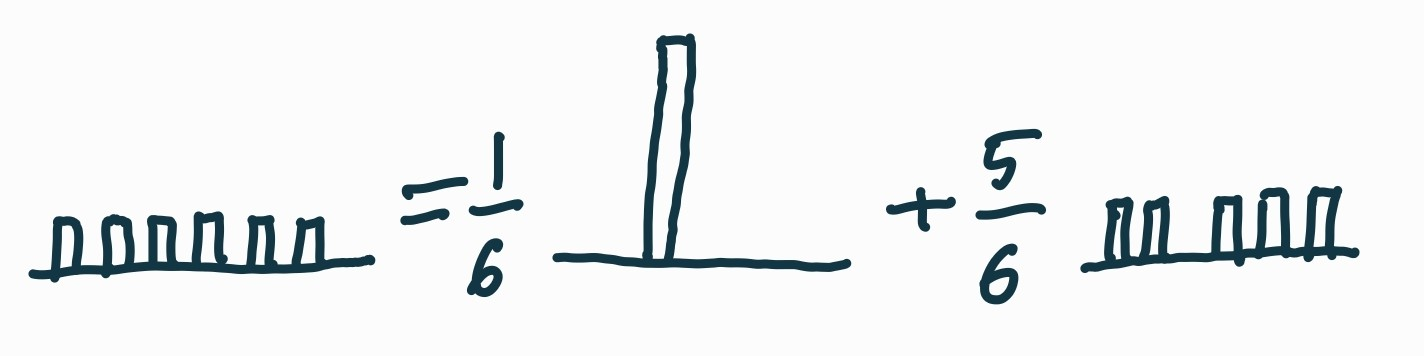
\includegraphics[width=0.6\textwidth]{tempimages/Fraction.jpg}
\end{figure}

First we define the \textbf{fraction} of one element within another. For example, suppose $\ens$ is a uniform distribution for a six-faced die. Suppose $\ens[a]$ represents the outcome 3 with $100\%$ probability. Then $\ens$ can be understood as $\ens = \frac{1}{6} \ens[a] + \frac{5}{6} \ens[b]$ where $\ens[b]$ is the uniform distribution over the outcomes 1,2,4,5 and 6. Note that $\frac{1}{6}$ is the highest coefficient we can put in front of $\ens[a]$ in a convex combination and have $\ens$ as a result, which coincides with the probability of obtaining 3 from a uniform distribution over six outcomes. That is what we define the fraction of $\ens[a]$ in $\ens$ to be.

\begin{mathSection}
	\begin{defn}
		Let $\ens, \ens[a] \in \Ens$ be two ensembles. The \textbf{fraction} of $\ens[a]$ in $\ens$ is the greatest mixing coefficient for which $\ens$ can be expressed as a mixture of $\ens[a]$. That is, $\size_{\ens}(\ens[a]) = \sup(\{ p \in [0,1] \, | \, \exists \, \ens[b] \in \Ens \text{ s.t. }  \ens = p \ens[a] + \bar{p} \ens[b] \})$.
	\end{defn}
\begin{figure}[H]
	\centering
	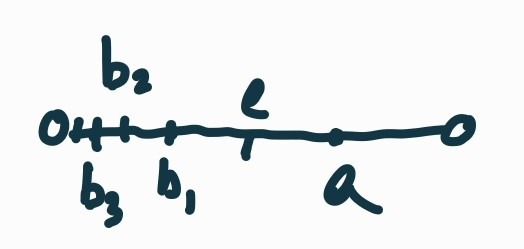
\includegraphics[width=0.4\textwidth]{tempimages/CapacitySupremum.jpg}
\end{figure}
	
	\begin{remark}
		We need to take the supremum as the maximum may not exist. For example, consider a discrete classical ensemble space and remove the extreme points. At the moment, there is no reason to rule out such space as unphysical.
	\end{remark}
	
	\begin{coro}
		Let $\ens, \ens[a] \in \Ens$, then $\size_{\ens}(\ens[a]) = 0$ if and only if $\ens[a]$ is not a component of $\ens$.
	\end{coro}
	
	\begin{proof}
		Note that $\ens[a]$ is a component of $\ens$ if we can write $\ens = \lambda \ens[a] + \bar{\lambda} \ens[b]$ for some $\lambda \in (0,1]$ and $\ens[b] \in \Ens$. In this case, $\size_{\ens}(\ens[a]) \geq \lambda > 0$. Conversely, if $\size_{\ens}(\ens[a]) > 0$ we can find $\size_{\ens}(\ens[a]) \geq \lambda > 0$ such that $\ens = \lambda \ens[a] + \bar{\lambda} \ens[b]$ for some $\ens[b] \in \Ens$.
	\end{proof}
\end{mathSection}

\begin{figure}[h]
	\centering
	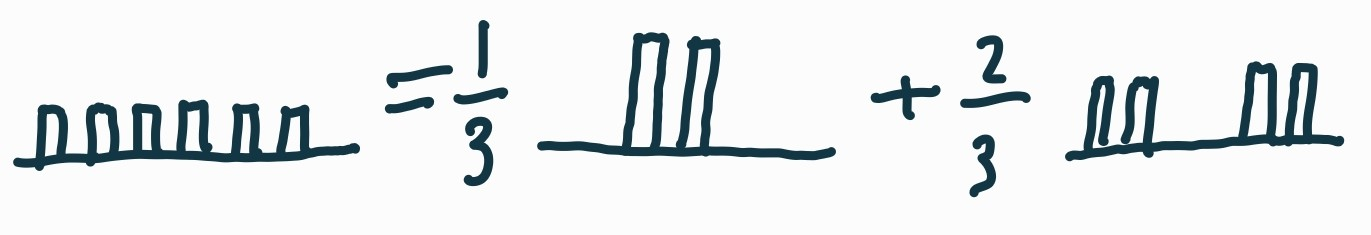
\includegraphics[width=0.6\textwidth]{tempimages/FractionCapacity.jpg}
\end{figure}

We now define \textbf{fraction capacity} of a set of ensembles for another ensemble. Like before, suppose $\ens$ is a uniform distribution for a six-faced die, but now take $A = \{ \ens[a], \ens[b] \}$ as, respectively, the outcomes $3$ and $4$ with $100\%$ probability. Then $\ens$ can be understood as $\ens = \frac{1}{3} \left(\frac{1}{2} \ens[a] + \frac{1}{2} \ens[b] \right) + \frac{2}{3} \ens[c]$, where $\ens[c]$ is the uniform distribution over outcomes 1,2,5 and 6. Again, note that $\frac{1}{3}$ is the highest coefficient we can put in front of any convex combinations of elements of $A$, and still make a convex combination that has $\ens$ as a result. That is what we define the fraction capacity of $A$ for $\ens$ to be.

The fraction capacity, then, defines how much of the ensemble $\ens$ can be constructed with elements of $A$. The term capacity is used first because, intuitively, it tells us how much $A$ can hold, and second because capacity is a name used to describe non-additive measures. The fraction capacity, in fact, has several nice properties. First, its value is always between zero and one, since the coefficient of a convex combination must be so bound. Second, it is monotone in the sense that if $A$ gets bigger, the fraction capacity cannot decrease. Third, it is subadditive, meaning that the fraction capacity of the union of two sets must be the sum of the respective fraction capacities or less. Fourth, it is continuous. Note that if subadditivity is replaced by additivity, these are exactly the defining properties of a probability measure, since additivity and continuity are equivalent to $\sigma$-additivity.

\begin{mathSection}
	\begin{defn}
		Let $\ens \in \Ens$ be an ensemble and $A \subseteq \Ens$ a Borel set. The \textbf{fraction capacity} of $A$ for $\ens$ is the biggest fraction achievable with convex combinations of $A$. That is, $\fcap_{\ens}(A) = \sup(\size_{\ens}(\hull(A))\cup\{0\})$.
	\end{defn}
	
	\begin{coro}
		The fraction capacity uniquely identifies an ensemble. That is, let $\ens[a], \ens[b] \in \Ens$ such that $\ens[a] \neq \ens[b]$. Then $\fcap_{\ens[a]} \neq \fcap_{\ens[b]}$.
	\end{coro}
	
	\begin{proof}
		Note that $\ens = 1 \ens[a] + 0 \ens[b]$ if and only if $\ens = \ens[a]$. Therefore, let $\ens[a], \ens[b] \in \Ens$ such that $\ens[a] \neq \ens[b]$. We have $\fcap_{\ens[a]}(\{\ens[a]\}) = 1$ and $\fcap_{\ens[b]}(\{\ens[a]\}) \neq 1$. Which means $\fcap_{\ens[a]} \neq \fcap_{\ens[b]}$.
	\end{proof}
	
	\begin{prop}
		The fraction capacity for an ensemble is a set function that is
		\begin{enumerate}
			\item non-negative and unit bounded: $\fcap_{\ens}(A) \in [0,1]$
			\item monotone: $A \subseteq B \implies \fcap_{\ens}(A) \leq \fcap_{\ens}(B)$
			\item subadditive: $\fcap_{\ens}(A \cup B) \leq \fcap_{\ens}(A) + \fcap_{\ens}(B)$
			\item continuous from below: $\fcap_{\ens}(\lim\limits_{i \to \infty} A_i) = \lim\limits_{i \to \infty} \fcap_{\ens}(A_i)$ for any increasing sequence $\{A_i\}$
			\item continuous from above: $\fcap_{\ens}(\lim\limits_{i \to \infty} A_i) = \lim\limits_{i \to \infty} \fcap_{\ens}(A_i)$ for any decreasing sequence $\{A_i\}$
		\end{enumerate}
	\end{prop}
	
	\begin{proof}
		1. The fraction capacity takes a subset of $\Ens$ and returns a real value and is therefore a set function. The mixture coefficients are real values between zero and one. The supremum of a set of numbers between zero and one is between zero and one, and therefore the fraction capacity for an ensemble is non-negative and unit bounded.
		
		2. The $\hull$ is a monotone function. The image of a set through a map is a monotone function. The supremum is a monotone function. Therefore the fraction capacity is a monotone function.
		
		3. Let $A, B \subseteq \Ens$ and let $p \in [0,1]$ such that $\ens = p \ens_1 + \bar{p} \ens_2$ for some $\ens_1 \in \hull(A \cup B)$ and $\ens_2 \in \Ens$. Since $\ens_1 \in \hull(A \cup B)$, we can write $\ens_1 = \lambda \ens[a] + \bar{\lambda} \ens[b]$ for some $\lambda \in [0,1]$, $\ens[a] \in A$ and $\ens[b] \in B$. Therefore we have $\ens = p \lambda \ens[a] + p \bar{\lambda} \ens[b] + \bar{p} \ens_2$. By the definition of fraction capacity, we must have $p\lambda \leq \fcap_{\ens}(A)$ and $p\bar{\lambda} \leq \fcap_{\ens}(B)$, therefore $p = p\lambda + p\bar{\lambda} \leq \fcap_{\ens}(A) + \fcap_{\ens}(B)$. 	Since $\fcap_{\ens}(A \cup B)$ is the supremum for a set of $p$s for which the expression always holds, we have $\fcap_{\ens}(A \cup B) \leq \fcap_{\ens}(A) + \fcap_{\ens}(B)$. The fraction capacity is subadditive.
		
		4. Let $\{A_i\} \subseteq \Sigma_{\Ens}$ be an increasing sequence. That is $A_i \subseteq A_{i+1}$ for all $i$. Given that the fraction capacity is monotone, $\{\fcap_{\ens}(A_i)\}$ is an increasing sequence. Note that $\fcap_{\ens}(A_i) \leq 1$ for all $i$, therefore the sequence will have an upper bound which will coincide with the limit. Let $A = \lim\limits_{i \to \infty} A_i$. We have $A = \bigcup A_i$ and $A_i \subseteq A$ for all $i$. Since fraction capacity is monotone, we have $\fcap_{\ens}(A_i) \leq \fcap_{\ens}(A)$ for all $i$ and therefore $\lim\limits_{i \to \infty} \fcap_{\ens}(A_i) \leq \fcap_{\ens}(A)$. Suppose $\lim\limits_{i \to \infty} \fcap_{\ens}(A_i) < \fcap_{\ens}(A)$. Then there would be an $\ens[a] \in \hull(A)$ such that $\size_{\ens}(\ens[a]) > \size_{\ens}(\ens[b])$ for all $\ens[b] \in \hull(A_i)$ for all $i$. But if $\ens[a] \in \hull(A)$, then it is the limit of a sequence of convex combination $\ens[c]_k$ of finitely many elements of $A$. We Then we will be able to find a $\hat{k}$ such that $\size_{\ens}(\ens[c]_{\hat{k}}) > \size_{\ens}(\ens[b])$ for all $\ens[b] \in \hull(A_i)$ for all $i$. Given that $\{A_i\}$ is an increasing sequence, there will be a $A_k$ that will contain those finitely many elements, and therefore $\ens[c]_{\hat{k}} \in \hull(A_k)$ which is a contradiction. Therefore $\lim\limits_{i \to \infty} \fcap_{\ens}(A_i) = \fcap_{\ens}(A)$.
		
		5. The previous argument works in the same way for decreasing sequences by inverting the order.
	\end{proof}
\end{mathSection}

\begin{conj}
	The fraction capacity is additive over sets whose convex closures are separate. Therefore it is additive over orthogonal sets.
\end{conj}

\begin{conj}
	The fraction capacity is $\sigma$-subadditive. That is, $\fcap_{\ens}(\bigcup A_i) \leq \sum_i \fcap_{\ens}(A_i)$.
\end{conj}

\begin{remark}
	In \href{https://link.springer.com/book/10.1007/978-3-319-30690-2}{Set Functions, Games and Capacities in Decision Making}, it is claimed that finite additivity plus continuity implies $\sigma$-additivity. The conjecture is that this generalizes to $\sigma$-subadditivity.
\end{remark}

\subsection{Topological measures}
Before showing when and how the fraction capacity reduces to a standard probability measure, we need to find which requirements a measure must satisfy to describe a well-posed physical problem. The issue is that the set of all probability measures defined over a space is too broad. Here we try to find the correct relationship a measure should have with respect to the topology of the space mathematically, which physically captures its relationsihp with experimental verifiability.

If we restrict ourselves to the real line, given the Lebesgue measure $\mu$, \href{https://en.wikipedia.org/wiki/Lebesgue%27s_decomposition_theorem}{Lebesgue's decomposition theorem} assures us that every measure $\nu$ can be divided into these three components: an \href{https://en.wikipedia.org/wiki/Absolute_continuity#Absolute_continuity_of_measures}{absolutely continuous} part $\nu_{ac}$ with respect to the Lebesgue measure (i.e. $\nu_{ac}(U)=0$ for all sets $U$ for which $\mu(U)=0$), a pure point part $\nu_{pp}$ (i.e. there is a set of countable points $\{x_i\}$ such that $\nu_{pp}(\{x_i\})=0$) and a singular continuous part $\nu_{sc}$ (i.e. $\mu(\{x\})=0$ for all $x$ and there is a set $U$ such that $\mu(U)=0$ and $\nu_{sc}(U^{\complement})=0$).

To make this more concrete, let us assume that we are working on phase space, $\mu$ is the Liouville measure, which in statistical mechanics quantifies the states in a region, and $p$ is a probability measure. If $p$ is absolutely continuous with respect to $\mu$, it means that if a region has no states, it will have zero probability. This is the requirement under which the \href{https://en.wikipedia.org/wiki/Radon%E2%80%93Nikodym_theorem}{Radon-Nikodym theorem} applies and a probability density $\frac{dp}{d\mu}$ exists. Without this requirement, for example, the entropy cannot even be defined. On physics grounds, this requirement makes a lot of sense. A pure point measure would correspond to the case where the probability is concentrated into a few isolated points. In physics, these are often represented with delta functions. There is an inherent unphysicality of these measures: if we really have a continuum, it would make no sense to say that we are are able to prepare an exact value with certainty. We are essentially saying that we are able to concentrate the whole distribution on a set that is not experimentally verifiable (i.e. it is a closed set with no interior) and contains no states (i.e. the Liouville measure is zero). Yet, there are some cases where the distribution is over real values, but only certain values are allowed. For example, the mass spectrum for particles or the energy spectrum for a bound quantum system can only take certain values. In this case, the Lebesgue measure is the one that is meaningless, because the region in between the allowed value contains no physically meaningful cases. A singular continuous measure may be something physically irrelevant, like the \href{https://en.wikipedia.org/wiki/Cantor_distribution}{Cantor distribution} which is defined only on a Cantor set, but it may also represent a constrained distribution. For example, a uniform distribution over the surface of a sphere, if defined over three dimensional space, would have support on a measure zero set, and have zero probability at every point. The issue, again, is that the imposition of the constraint has to be applied to the whole mathematical structure, not just the probability measure.

Physically, we see that the requirement of experimental verifiability poses constraints on the measure. Mathematically, experimental verifiability is captured by the topology. Therefore the question is: when can we way that a measure is compatible with a topology? That is, instead of having relationships between measures, which ignore the topology, we should have a direct relationship between each measure and the topology. If two measures are compatible with the topology, then they should be automatically well-behaved with respect to each other.

Let us step back and think more broadly. Recall that an open set corresponds to an experimentally verifiable statement. Imagine we prepared a distribution over some variable, and have a test that tells us whether the value of an instance is within a specific range $U$. Then the open set $U$ corresponds to the positive outcome of the test. The exterior $\exterior(U)$ corresponds to the negative outcomes of our test. The boundary $\partial U$ corresponds to those cases we are not able to adjudicate experimentally: they are not in $U$, but are too close to $U$ to discern from $U$. That is, there is no test that can tell us we have an element of $\partial U$, these cases are not experimentally verifiable. Assigning a non-zero probability or count of states to these sets, then, would be physically unjustifiable. On physical grounds, $\mu(\partial U) = 0$ for every open set $U$.

The requirement now depends on the topology, and is satisfied by the standard measures on their respective topology. For example, if we have a discrete topology, every open set is also closed, therefore the boundary of every open set is the empty set, which will have measure zero. On the other hand, if we have the real line with the standard topology, the boundary of an open interval is the two extreme points, which will have measure zero. If a probability measure is absolutely continuous with respect to the Lebesgue measure, it will have measure zero over all boundaries of all open sets as well. In fact, that requirement is enough to show it is absolutely continuous.

To sum up, given a topological space $X$, we are interested in measures that are compatible with its topology. This requirement can be simply stated: the measure over an open set has to be equal to the measure on its closure. 

\begin{mathSection}
\begin{defn}
	Let $X$ be a topological space. We say a measure $\mu : \Sigma_X \to \mathbb{R}$ is compatible with the topology if $\mu(U) = \mu(\bar{U})$ for every open set $U$.
\end{defn}
\begin{justification}
	Recall that if $X$ is a topological space that represents an experimental domain, each open set represents a verifiable statement. If a measure quantifies a physically well-defined quantity associated to the statement, it has to be associated only to the part of the statement that can be experimentally verified or falsified. The undecidable part, then, is physically indistinguishable from an empty set and therefore have zero measure. This means we are justified to assume the measure on an open set is the same as the measure on its closure.
\end{justification}
\end{mathSection}

We stress that $\mu(U) = \mu(\overline{U})$ is not necessarily true for all Borel sets, just for open sets. Consider, in fact, the set of rationals $\mathbb{Q}$ as a subset of the reals $\mathbb{R}$. This is a measure zero subset whose closure is the whole space. Therefore, if $p$ is a probability measure over the reals, we would have $p(\mathbb{R}) = p(\overline{\mathbb{Q}}) = p(\mathbb{Q})$ which would mean that the probability is all concentrated on a set of measure zero, which is exactly what we do not want. On the other hand, we are also not saying that all sets of measure zero are boundaries of open sets. The set of rationals is not the boundary of an open set. Additionally, since all boundaries of open sets have no interior (i.e. are nowhere dense sets), one may be tempted to say that all nowhere dense sets have measure zero. This, again, does not work. To better understand the requirement both mathematically and physically, let us find a bigger class of sets that will have the same property.

Conceptually, we are saying that it does not make sense to assign probability to non-termination. The prediction that a test will never terminate cannot be verified and we cannot gather statistics about it. Since the boundary of a set corresponds to the possibilities that are associated with an undefined outcome, the first instinct would be to simply say that any set that is a boundary of another set has zero probability. This does not work. Consider the statement \statement{the mass of the electron is rational in $eV$.} This statement corresponds to the rationals $\mathbb{Q}$ as a subset of the reals $\mathbb{R}$. Since the statement is undecidable, the associated test will never terminate. The boundary of $\mathbb{Q}$ is the whole $\mathbb{R}$, the whole space, which must have probability one. That is, we can never verify or falsify that a continuous quantity is exactly a rational or not as it would require infinite precision. The issue here is that the termination condition is specific to a particular set, to a particular statement. No set is intrinsically a boundary or not. However, if the boundary has no interior, it means that there is no additional test that can tell us whether we are in one of the non-terminating conditions. In the previous case, we know a priori that the test will never terminate in any case. Therefore, if we are able to predict that the test for a particular statement will never terminate, and we are able to verify that prediction with a verifiable statement, we would be able to say that \statement{there is a probability $p$ that the test will not terminate}. The correct characterization, then, is that a boundary set with an empty interior cannot be assigned non-zero probability.

Mathematically, this leads to the notion of a nicely bounded set, a set whose boundary is nowhere dense. Measures that behave nicely with open sets are exactly those that behave nicely with nicely bounded sets.

\begin{mathSection}
\begin{defn}
	Let $X$ be a topological space. A set $A \subseteq X$ is \textbf{nicely bounded} if its boundary is nowhere dense.
\end{defn}

\begin{coro}
	The following statements are equivalent:
	\begin{enumerate}
		\item $A$ is nicely bounded
		\item $\overline{A} = \overline{\interior(A)}$
		\item $\exterior(A) = \exterior(\interior(A))$
	\end{enumerate}
\end{coro}

\begin{proof}
	To show that 1 and 2 are equivalent, consider a nicely bounded set $A$. Like any set, $X$ will be partitioned into the three disjoint sets $\interior(A)$, $\partial A$ and $\exterior(A)$. Let $U \supset \emptyset$ be a non-empty open set. Since $\interior(\partial A) = \emptyset$, either $U \subseteq \interior(A)$, $U \subseteq \exterior(A)$ or it will overlap with more than one of the regions. This means that any open set that is disjoint from the exterior is either already in the interior or the union of an open set and a set of limit points. Therefore any open set that is disjoint from the exterior is in the closure of the interior. Conversely, if $A$ and $\interior(A)$ have the same closure, then any open set in the closure must overlap with a set in the interior. Therefore there is no open set in the closure that is disjoint from the interior, and therefore the boundary has an empty interior.
	
	To show that 3 is equivalent to 2, note that the exterior is the complement of the closure. Therefore two sets have the same closure if and only if they have the same exterior.
\end{proof}

\begin{prop}
	Open and closed sets are nicely bounded. The complement of a nicely bounded set is nicely bounded. The intersection and the union of nicely bounded sets are nicely bounded. The closure of open sets under complement, finite intersection and finite union is a Boolean algebra $R_X$ of nicely bounded sets.
\end{prop}

\begin{proof}
	Let $A \subset X$ be an open set. Since $A$ is an open set, $A = \interior(A)$. Since $\partial A$ and $\interior(A)$ are disjoint, $\partial A$ and $A$ are disjoint. Let $U$ be an open set such that $U \subseteq \partial A$. Therefore $U$ must be disjoint from $A$. We also have $U \subseteq \partial A \subseteq \bar{A}$. Since $U$ is an open set, it will be a subset of the interior of the closure of $A$, which is $A$ since $A$ is an open set. Putting it all together, $U$ must be an open set that is disjoint from $A$ but also a subset of $A$. Therefore $U$ is the empty set. Therefore the interior of the boundary of $A$ must be the empty set, which means it is nowhere dense.
	
	Let $A$ be a nicely bounded set. Since the boundary of a set is equal to the boundary of its complement, the complement of $A$ must also be a nicely bounded set. A closed set is the complement of an open set, which is a nicely bounded set, therefore all closed sets are nicely bounded.
	
	Let $A, B \subseteq X$ be two nicely bounded sets. The boundary \href{https://proofwiki.org/wiki/Boundary_of_Union_is_Subset_of_Union_of_Boundaries}{satisfies} the property $\partial (A \cup B) \subseteq \partial A \cup \partial B$. The union of two nowhere dense sets is nowhere dense and \href{https://proofwiki.org/wiki/Subset_of_Nowhere_Dense_Subset_is_Nowhere_Dense}{a subset of a nowhere dense set is nowhere dense}. Therefore $\partial (A \cup B)$ is nowhere dense and $A \cup B$ is a nicely bounded set. Since complements and unions of nicely bounded sets are nicely bounded, by De Morgan intersections are nicely bounded as well.
	
	Let $R_X$ be the closure of open sets under complement, finite intersection and finite union. This forms a Boolean algebra as it is closed under the given operations and it includes $\emptyset$ and $X$. Moreover, since the algebra is generated from the open sets, which are nicely bounded, all sets will be nicely bounded.
\end{proof}

\begin{remark}
	Note that the algebra $R_X$ does not contain all the nicely bounded sets. Consider a circle in $\mathbb{R}^2$. Let $U$ be the open set of all the interior points and $B$ be the points on the circle at a rational angle. Now consider $A = U \cup B$: $U$ is the interior of $A$ and $B$ its boundary. The boundary is is nowhere dense, therefore $A$ is a nicely bounded set. However, we cannot generate $A$ with finite operations from open sets of $\mathbb{R}^2$.
\end{remark}

\begin{prop}
	Given a topological space $X$ and a measure $\mu$ on its Borel algebra, the following propositions are equivalent:
	\begin{enumerate}
		\item $\mu$ is compatible with the topology
		\item $\mu(A) = \mu(\bar{A})$ for any nicely bounded set $A$
		\item $\mu(A) = \mu(\interior(A))$ for any nicely bounded set $A$
		\item $\mu(\partial A) = 0$ for any nicely bounded set A
		\item $\mu(\interior(A)) + \mu(\exterior(A)) = \mu(X)$ for any nicely bounded set $A$
	\end{enumerate}
\end{prop}

\begin{proof}
	To show that 2 implies 1, every open set is a nicely bounded set. Therefore $\mu(A) = \mu(\bar{A})$ for all open sets.
	
	To show that 2, 3 and 4 are equivalent, first note that if $A$ is nicely bound then $\interior(A)$ is also nicely bound since $A$ and $\interior(A)$ have the same boundary. Given that $\bar{A} = \interior(A) \cup \partial A$ and $\interior(A) \cap \partial A = \emptyset$, we have $\mu(\bar{A}) = \mu(\interior(A) \cup \partial A) = \mu(\interior(A)) + \mu(\partial A)$. Given that $\interior(A) \subseteq A \subseteq \bar{A}$, $\mu(\interior(A)) \leq \mu(A) \leq \mu(\bar{A})$. Therefore $\mu(\interior(A)) = \mu(A) = \mu(\bar{A})$ if and only if $\mu(\partial A) = 0$.
	
	To show that 1 implies 4, note that if $A$ is a nicely bounded set, then $\interior(A)$ is an open set that has the same boundary as $A$. If $\mu$ is compatible with the topology, $\mu(\interior(A)) = \mu(\bar{A})$ which means $\mu(\partial A) = 0$.
	
	To show that 5 is equivalent to 4, first note that $X = \interior(A) \cup \partial A \cup \exterior(A)$ for any $A$. Also note that the interior, the exterior and the boundary are all disjoint. Therefore $\mu(X) = \mu(\interior(A)) + \mu(\partial A) + \mu(\exterior(A))$. Therefore $\mu(\partial A) = 0$ for any nicely bounded set if and only if $\mu(X) = \mu(\interior(A)) + \mu(\exterior(A))$.
\end{proof}
\end{mathSection}

Given that we are stressing the importance of the topology, one is led to ask: can we just define the measure purely in terms of the topology, with no reference to the Borel algebra? That is, can we define a measure-theoretic object that is purely topological? The answer is positive. Once the measure is defined on the open sets, it can first be extended to the algebra of nicely bounded sets and then to the whole Borel algebra.

\begin{mathSection}
\begin{defn}
	Let $X$ be a topological space. A \textbf{topological measure} is a set function $\mu$ over the topology that satisfies the following:
	\begin{enumerate}
		\item non-negative: $\mu(U) \geq 0$
		\item topologically additive: $\mu\left(\interior\left(\overline{\bigcup_{i \in I} U_i}\right)\right) = \sum_{i \in I} \mu(U_i)$ whenever $U_i \cap U_j = \emptyset$ for all $i\neq j$
		\item locally finite: for any $U$, we can find $V \in \textsf{T}_X$ such that $\emptyset \subset V \subseteq U$ and $\mu(V) < + \infty$.
	\end{enumerate}
	The measure is finite if $\mu(X) < \infty$.
\end{defn}

\begin{coro}
	Let $\mu$ be a topological measure, then the following are true:
	\begin{enumerate}
		\item the measure is monotone: $U \subseteq V$ implies $\mu(U) \leq \mu(V)$
		\item the empty set has zero measure: $\mu(\emptyset) = 0$
		\item $\mu(U) = \mu(\interior(\overline{U}))$ for every open set $U$.
	\end{enumerate}
\end{coro}

\begin{proof}
	For 1, let $U \subseteq V$ then $V = U \cup (V \setminus U)$ where $U$ and $(V \setminus U)$ are disjoint. This means that $U$ and $\interior(V \setminus U)$ are also disjoint. We have $\mu(V) = \mu(\interior(\overline{U \cup \interior(V \setminus U)})) = \mu(U) + \mu(\interior(V \setminus U)) \geq \mu(U)$.
	
	For 2, since $\emptyset$ is open, it is disjoint from itself and it is its own closure, $\mu(\emptyset) + \mu(\emptyset) = \mu(\interior(\overline{\emptyset\cup\emptyset}))= \mu(\emptyset)$. This means the empty set has either zero measure or infinite measure. Since the measure is monotone and locally finite, the empty set has zero measure.
	
	For 3, let $U$ be an open set. We have $\mu(U) = \mu(U) + \mu(\emptyset) = \mu(\interior(\overline{U\cup\emptyset}))= \mu(\interior(\overline{U}))$.
\end{proof}

\begin{thrm}[Topological measure extension theorem]
	Let $X$ be a topological space and $\mu$ a topological measure on that space. Then there exists a measure $\overline{\mu}$ defined on the Borel algebra such that $\left.\overline{\mu}\right|_{\textsf{T}_X} = \mu$. If $X$ is second countable or if $\mu$ is finite the extension is unique.
\end{thrm}

\begin{proof}
	The strategy is first to extend the topological measure $\mu$ to a pre-measure $\mu'$ over the algebra of nicely bounded sets generated by the open sets and then use \href{https://en.wikipedia.org/wiki/Carath%C3%A9odory's_extension_theorem}{Carathéodory's extension theorem} to extend to a measure $\bar{\mu}$ on the whole Borel algebra.
	
	First we show that if we want to extend the topological measure $\mu : \mathsf{T}_X \to [0,+\infty]$ to a pre-measure $\mu' : R_X \to [0,+\infty]$ over $R_X$, the algebra generated by closing the open sets under complement and finite intersection, the pre-measure of a closed set must be the same as the topological measure of its interior. That is, $\mu'(U) = \mu(\interior(U))$ for any closed set $U$. Let $U$ be a closed set and $V$ an open superset of $U$. Then $W = V \setminus U = V \cap U^{\complement}$ is an open set since it is the intersection of two open sets. Since $\mu'$ must be additive, we must have $\mu(V) = \mu'(V) = \mu'(U) + \mu'(W) = \mu'(U) + \mu(W)$. Note that $\interior(U)$ and $W$ are two disjoint open sets, therefore we have $\mu(\interior(U)) + \mu(W) = \mu(\interior(\overline{W \cup \interior(U)})) = \mu(\interior(\overline{W \cup U})) = \mu(\interior(\overline{V})) = \mu(V)$. Therefore $\mu'(U) = \mu(\interior(U)) = \mu'(\interior(U))$.
	
	Now we show that for any nicely bounded set $U$, $\mu'(U) = \mu'(\overline{U}) = \mu'(\interior(U)) = \mu(\interior(U))$. For a generic set, we have $\interior(U) \subseteq U \subseteq \overline{U}$. Therefore $\mu'(\interior(U)) \leq \mu'(U) \leq \mu'(\overline{U})$. Since $\interior(U)$ is an open set, we have $\mu'(\interior(U)) = \mu'(\interior(\overline{\interior(U)}))$. Since $U$ is nicely bounded, $\overline{U} = \overline{\interior(U)}$ and therefore $\mu'(\interior(\overline{\interior(U)})) = \mu'(\interior(\overline{U}))$. Since $\overline{U}$ is a closed set, $\mu'(\interior(\overline{U})) = \mu'(\overline{U})$. Putting it all together, $\mu'(\interior(U)) = \mu'(\overline{U})$. Since $\mu'(U)$ must be between the two values, $\mu'(U) = \mu'(\interior(U)) = \mu'(\overline{U}) = \mu(\interior(U))$.
	
	We can therefore extend the topological measure $\mu$ to a pre-measure $\mu'$ over all nicely bounded sets simply by setting $\mu'(U) = \mu(\interior(U))$. Since the interior of disjoint sets is disjoint, the pre-measure will preserve $\sigma$-additivity. Therefore the extension is a pre-measure on the algebra of nicely bounded sets generated from the open sets. This satisfies the prerequisites of Carathéodory's extension theorem, and it can therefore be extended to measure $\bar{\mu} : \Sigma_X \to [0,+\infty]$ over the full Borel algebra $\Sigma_X$.
	
	The extension is unique if the pre-measure $\mu'$ is $\sigma$-finite, which means, for example, that we can find a countable cover of the space where each open set is finite. Note that if $X$ is second countable, and since the measure is locally finite, we are going to be able to find a countable basis of the space where each element of the basis is finite. Therefore we are guaranteed $\sigma$-finite. If the topological measure is finite, then it is $\sigma$-finite regardless of the space.
\end{proof}

\begin{conj}
	Let $X$ be a topological space and $\mu : \Sigma_X \to [0,+\infty]$ be a $\sigma$-finite measure compatible with the topology. Then $\left.\mu\right|_{\textsf{T}_X}$ is a topological measure and $\mu$ is its unique extension.
\end{conj}
\end{mathSection}

\subsection{Flats and affine combinations}

Having seen the type of classical probability measure each ensemble should reduce to, we now need to identify the correct closure condition for a set of ensembles to form a space of probability measures. Roughly speaking, we want to be able to think of the set of ``all'' the probability distributions over a set of cases. We have to clarify what we mean by ``all.''

Requiring the set of probability measures to be closed under convex combinations is not enough. The cut triangle \ref{pm_es_cutTriangle}, for example, is a subset of a discrete classical ensemble space where not all ensembles can be understood as a unique convex combination of the extreme points, precisely because some cases are missing. This convex subset is leaving out some ensembles, making a classical space not look classical. On the other hand, if we take a Bloch ball, we can take three points on the surface. These would form a triangle, which could be understood as a discrete classical probability space. Here the convex closure is leaving out some ensembles, making a non-classical space look classical. Therefore we first have to understand what the correct closure is before we can determine whether it forms a set of classical probability measures or not.

As an early attempt, we considered extending the closure to both mixtures and components. That is, closure on the mixtures would require $\ens[a] = p \ens[b] + \bar{p} \ens[c]$ to be in the set if both $\ens[b]$ and $\ens[c]$ are present. Closure on the components would also require $\ens[b]$ and $\ens[c]$ to be in the set if $\ens[a]$ is present. This seems to take too much in. In quantum mechanics, for example, a single mixed state would bring in all the mixed states in the smallest subspace that contains it. The problem is that we would never be able to carve out the spaces of classical probability measures that are associated with each quantum measurement context.

The correct closure seems to be to include all affine combinations. That is, if $\ens[a] = p \ens[b] + \bar{p} \ens[c]$ and two of the ensembles are in the set, then the other one is in the set as well. This allows us to get all the ensembles in the same hyperplane. We call this a flat. In the triangle example, the only flats available are the single vertexes, each side and the whole triangle. For the Bloch ball, if we took two elements, we would get the whole segment that connects them and extends to the surface. But if we get three points, we get a circle, which is not a simplex. This affine closure, essentially, allows us to remove ``ensembles from each other'' as much as possible, so that we can get to their most distinct, most separate, form.

% Reviewed with Christine start

\begin{mathSection}
\begin{defn}
	A \textbf{simplex} is a subset $U \subset \mathbb{R}^n$ that is the hull of finitely many affinely independent points. That is, $U = \hull(\{x_i\}_{i=0}^{n})$ such that $\{x_i - x_0\}_{i=1}^{n}$ are linearly independent.
\end{defn}

\begin{defn}
	A \textbf{flat} $A \subseteq \Ens$ is a closed convex subset that contains all lines between all elements. That is, for any $\ens[a], \ens[b] \in A$, $A$ also contains the line that contains $\ens[a]$ and $\ens[b]$. Given a set $U \subseteq \Ens$, the \textbf{flat closure} of $U$ is the smallest flat that contains $U$. A flat is \textbf{finite} if it can be generated by a finite number of elements. An $n$-flat is a flat that must be generated by a set with at least $n$ elements.
\end{defn}

\begin{figure}[H]
	\centering
	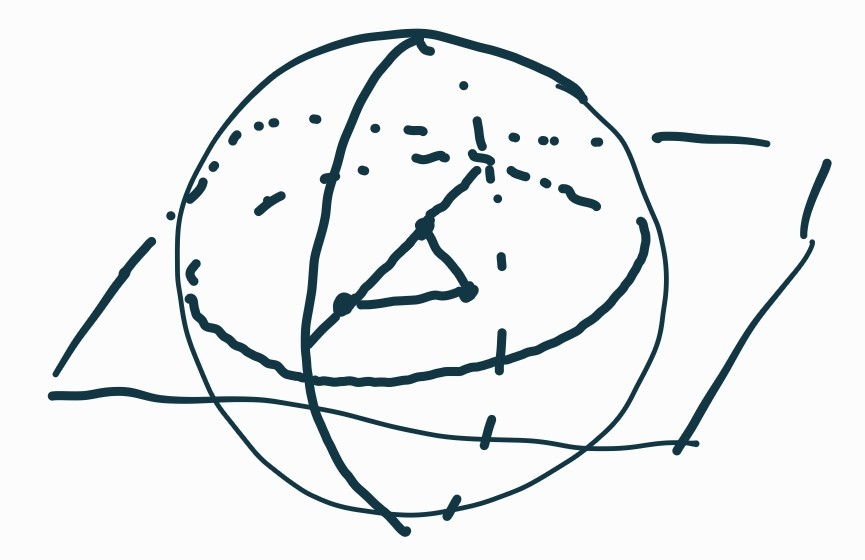
\includegraphics[width=0.4\textwidth]{tempimages/FlatVsConvex.jpg}
	\caption{Flat vs convex set. The ball is the ensemble space. The triangle represents a convex subset. The disc containing the triangle is the flat closure of the triangle. The plane is the affine closure of the triangle.}
\end{figure}


\begin{prop}
	A flat includes all possible affine combinations of elements of $\Ens$ that are contained in $\Ens$. The flat closure of $U \subseteq \Ens$ is the intersection of $\Ens$ with the affine closure of $U$ in the embedding vector space.
\end{prop}

\begin{proof}
	Let $A \subseteq \Ens$ be a flat and let $V$ be the real vector space that embeds $\Ens$. A line between two elements $\ens[a], \ens[b] \in A$ can be extended in $V$ and can be written as $\ens[a] + x \left(\ens[b] - \ens[a]\right)$ with $x \in \mathbb{R}$. Therefore any ensemble that can be written as an affine combination of two ensembles in $A$ is an element of the flat. Recursively, this means that any ensemble that can be written as an affine combination of finitely many ensembles in $A$ is also in the flat. Moreover, since the flat is a closed set, it will also include all its limits. Therefore every affine combination of $A$ that is also an element of $\Ens$ is in $A$, which means $A$ is the intersection of an affine subspace of the embedding vector space and the ensemble space.
	
	Now let $U \subseteq \Ens$ be a set of ensembles. The affine closure of $U$ will be an affine subspace of the embedding vector space. The flat closure will be the intersection of the affine closure with $\Ens$. Since the affine closure is the smallest closed affine subspace that contains $U$, its intersection with $\Ens$ will be the smallest flat that contains $U$, which is the flat closure of $U$.
\end{proof}

\begin{conj}
	An $n$-flat is a simplex if and only if its $3$-flats are simplexes (i.e. triangles).
\end{conj}

\begin{remark}
	In classical discrete ensemble spaces, any flat is a simplex. In classical continuous ensemble spaces, infinite dimensional flats will depend on what limits are allowed. In a quantum ensemble space, if we take three ensembles inside a Bloch ball, the corresponding flat will be a circle. If we take three orthogonal pure states, however, the corresponding flat will be a simplex.
\end{remark}
\end{mathSection}

\subsection{Classical probability contexts}

Now that we have identified the correct closure, we need to find the right characterization of a flat to identify a classical probability context: a set of ensembles that can be characterized by a family of classical probability measures. For finite discrete spaces, we want to recover the notion of a simplex. In a simplex, every element has a single decomposition in terms of extreme points. This characterization does not work in infinite dimensions as there are no extreme points. As we saw before, the pure point probability measures are not, in general, continuous with respect to the topology. The trick, again, is being able to express this lack of multiple decompositions for finite mixtures.

%A classical probability context will be a set of ensembles that we will map to a space of measures. From the ensembles we will need to define the points over which the probability are defined, the spectrum of the context (in analogy to the spectrum of a linear operator). The general idea is that these will be limits of ensembles that become more and more concentrated, which will be characterized using tools from order theory and topology. Once the spectrum is defined, we will use the fraction capacity to define the probability measure over the topology of the spectrum.

%Technical details aside, we want definitions that capture the intuition of spaces of classical probability distributions in a way that works well for infinite dimensional spaces, is compatible with both discrete and continuous classical ensemble spaces but also with measurement contexts in quantum ensemble spaces. It is instructive to go through some of the different attempts to understand why we settled on these definitions, so that one can understand why they work.

\begin{mathSection}
\begin{defn}
	An ensemble is \textbf{decomposable} if it can be expressed as a mixture of two ensembles. An ensemble is \textbf{separately/orthogonally decomposable} if it can be expressed as a mixture of two separate/orthogonal ensembles. An ensemble is \textbf{separately multidecomposable} if it can be expressed as two decompositions where a component of one is separate from both components of the other. That is, $\ens = p \ens[a]_1 + \bar{p} \ens[a]_2 = \lambda \ens[b]_1 +\bar{\lambda} \ens[b]_2$ and either $\ens[a]_1 \separate \ens[b]_j$ or $\ens[a]_2 \separate \ens[b]_j$.
\end{defn}

\begin{figure}[H]
	\centering
	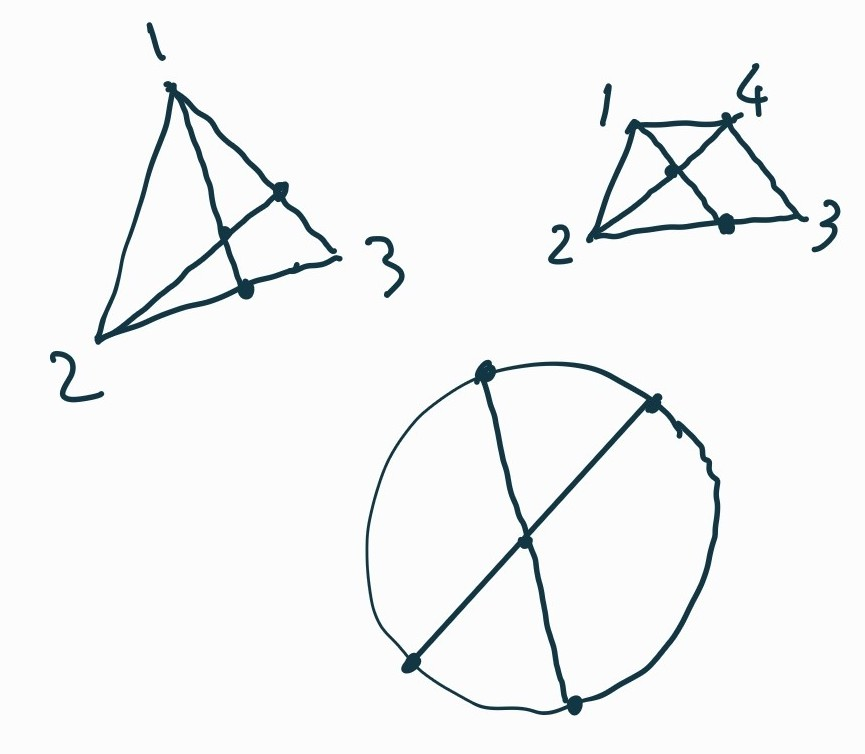
\includegraphics[width=0.4\textwidth]{tempimages/MultipleDecomposition.jpg}
\end{figure}

\begin{remark}
	Take a classical discrete space for three points which is a triangle (simplex). The only three elements that are not decomposable are the extreme points. Mixtures of two points are decomposable and are also separately decomposable in only one way. Mixtures of three points are also separately decomposable, but in multiple ways: as a mixture of $\ens_1$ and a mixture of $\ens_2$ and $\ens_3$, or as a mixture of $\ens_2$ and a mixture of $\ens_1$ and $\ens_3$. Note, however, that they are not separately multidecomposable as the different components are not separate.
	
	Take a Bloch ball for quantum mechanics. All the elements of the surface are not decomposable and they are all pairwise separate. The middle point can be seen as the equal mixture of any pair of opposite points. Therefore the middle point, as well as any other point not on the surface, is not only separately decomposable but also multidecomposable.
	
	To see why we require only one component to be separate from the other two, consider the cut triangle. Here we can have multiple decompositions where not all elements are separate.
\end{remark}

\begin{figure}[H]
	\centering
	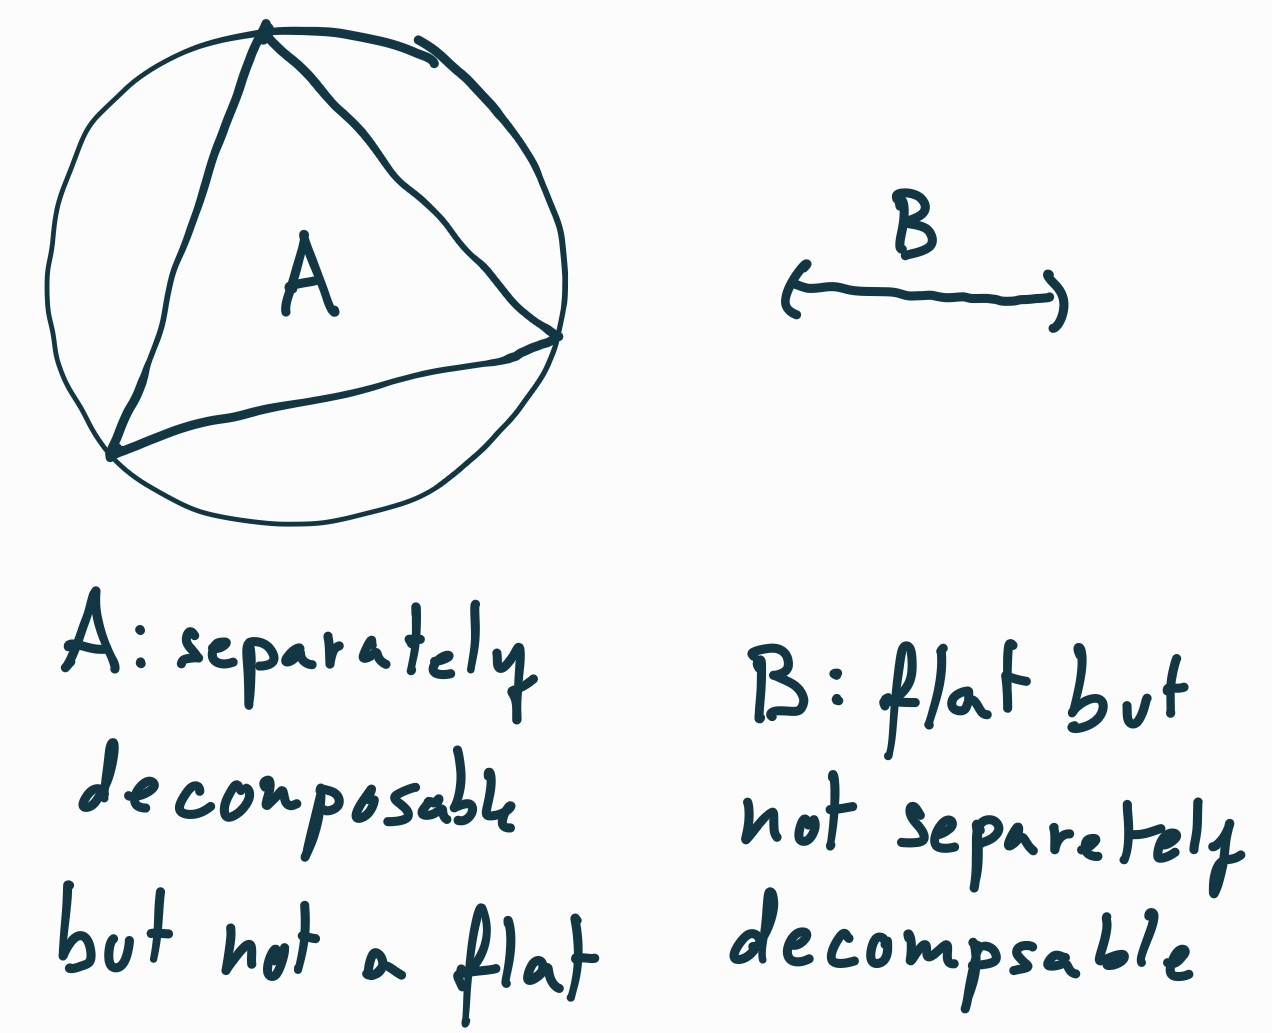
\includegraphics[width=0.4\textwidth]{tempimages/SeparableButNotFlat.jpg}
\end{figure}

\begin{remark}
	A convex set that is separately decomposable is not necessarily a flat (i.e. triangle within a sphere). A flat is not necessarily separately decomposable (i.e. open segment as a whole is a flat, but is not separately decomposable).
\end{remark}

\begin{defn}
	Let $\Ens$ be an ensemble space. A \textbf{classical probability context} is a flat $C \subseteq \Ens$ where each decomposable element in $C$ is separately decomposable in $C$ but not separately multidecomposable in $C$.
\end{defn}

\begin{conj}
	A flat $C \subseteq \Ens$ is a classical probability context if and only if every decomposable element is separately decomposable and mixtures preserve separateness in $C$. That is, if $\ens \separate \ens[a]$ and $\ens \separate \ens[b]$, then $\ens \separate p\ens[a] + \bar{p} \ens[b]$ in $C$ for all $\ens, \ens[a], \ens[b] \in C$ and $p \in [0,1]$.
\end{conj}

\begin{conj}
	A convex subset $U \subseteq \Ens$ is a classical probability context if and only if all finite flats are simplexes.
\end{conj}

\begin{prop}
	Let $C \subseteq \Ens$ be a classical probability context. Let $U \subseteq C$ be a set of ensembles. Then $A=U^\separate=\{ \ens[a] \in C \, | \, \forall \ens \in U, \ens[a] \separate \ens \}$ and $B=(U^\separate)^\separate=\{ \ens[b] \in C \, | \, \forall \ens[a] \in A, \ens[b] \separate \ens[a] \}$ are two probability contexts such that $C = \hull(A \cup B)$.
\end{prop}

\begin{proof}
	First we show that $C$ contains only three types of ensembles: those that are limits of convex mixtures of $A$, those that are limits of convex mixtures of $B$ and those that are limits of convex mixtures of both $A$ and $B$. Any ensemble in $C$ is one of these three types. For $\ens[c] \in C$ to not be a mixture of $A$ or $B$, then $\ens[c]$ cannot be in either $A$ or $B$. This means that it must be separate from both $A$ and $B$. But $B$ contains all the elements that are separate from $A$, which is a contradiction. Since separate multidecomposition is forbidden, an ensemble $\ens$ cannot be written both as a convex combination of $A$ and as a convex combination with an element of $B$. This would yield two decompositions in which one component, the one chosen from $B$, is separate from all the components of the other. This means that an element of $C$ is either a mixture of $A$, a mixture of $B$ or a mixture of both $A$ and $B$.
	
	Now we show that both $A$ and $B$ are convex sets. Since a mixture of $A$ can only be expressed as a mixture of components of $A$, it is separate from all elements of $B$. Therefore $A$ contains all its mixtures. With the same logic, $B$ will contain all its mixtures. The argument works for infinite convex combinations as well. If $\ens = \sum_{i=1}^{\infty} p_i \ens[a]_i$ with $p_i \in [0,1]$ and $\sum_{i=1}^{\infty} p_i = 1$, it can be understood as the limit of the series $\frac{p_1}{P_n} \ens[a]_1 + \frac{\bar{p}_1}{P_n} \sum_{i=2}^{n} p_i \ens[a]_i$ where $P_n = \sum_{i=1}^{n} p_i$. Therefore
	\begin{equation}
		\begin{aligned}
			\ens &= \sum_{i=1}^{\infty} p_i \ens[a]_i = \lim\limits_{n \to \infty}  \sum_{i=1}^{n} \frac{p_i}{P_n} \ens[a]_i = \lim\limits_{n \to \infty} \frac{p_1}{P_n} \ens[a]_1 + \lim\limits_{n \to \infty}\frac{\bar{p}_1}{P_n} \sum_{i=2}^{n} \frac{p_i}{\bar{p}_1} \ens[a]_i = p_1 \ens[a]_1 + \bar{p}_1 \sum_{i=2}^{\infty} \frac{p_i}{\bar{p}_1} \ens[a]_i \\
			&= p_1 \ens[a]_1 + \bar{p}_1 \hat{\ens[a]}_1
		\end{aligned}
	\end{equation}
	where $\hat{\ens[a]}_1 = \sum_{i=2}^{\infty} \frac{p_i}{\bar{p}_1} \ens[a]_i$. Since $\ens$ and $\ens[a]_1$ are elements of the ensemble space, the series converges to $\hat{\ens[a]}_1$, which is in the hull of $A$. It will also be an element of $A$ because multidecompositions are forbidden.
	
	To see that $C$ is the hull of $A$ and $B$, note that all the elements in $C$ that are not already in $A$ or $B$ are the mixtures of $A$ and $B$. These are exactly added when taking the hull of $A \cup B$.
	
	Now we show that $A$ and $B$ are classical probability contexts. First we have to show that they are flats. Let $L$ be the line that connects two elements $\ens[a]_1, \ens[a]_2 \in A$. Take $\ens[a]_3 \in L$. If it is a mixture of $\ens[a]_1$ and $\ens[a]_2$ then it is an element of $A$. If $\ens[a]_1$ is a mixture of $\ens[a]_2$ and $\ens[a]_3$, since $\ens[a]_1$ cannot have a common component with $B$, and $\ens[a]_3$ is a component of $\ens[a]_1$, $\ens[a]_3$ cannot have components in $B$ as well. Therefore $\ens[a]_3$ must be a mixture of elements of $A$. Similarly if $\ens[a]_2$ is a mixture of $\ens[a]_1$ and $\ens[a]_3$. Therefore $A$ is a flat. Similarly, $B$ is a flat.
	
	Now we show that $A$, and by symmetry $B$, is a classical probability context. We have seen that $A$ is a flat. If an element of $A$ is decomposable in $A$ it is also decomposable in $C$ and is therefore separately decomposable in $C$. Because multidecomposability in $C$ is not allowed, it must be separately decomposable into elements of $A$. Lastly, if multidecomposability were allowed in $A$, it would also be allowed in $C$. Therefore it is not allowed in $A$. This means that $A$ is a classical probability context.
\end{proof}

\begin{figure}[H]
	\centering
	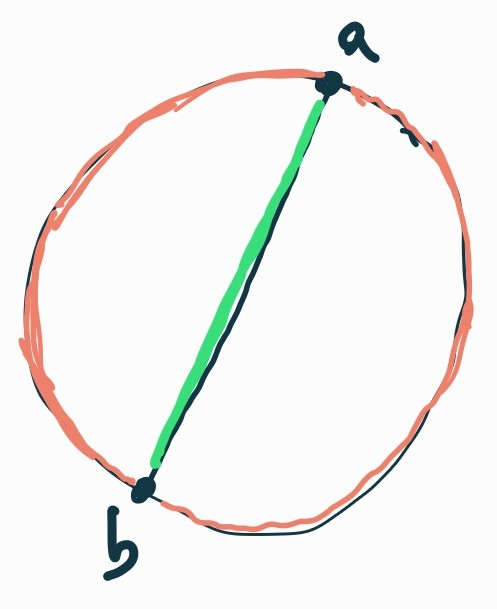
\includegraphics[width=0.25\textwidth]{tempimages/CounterexampleProbabilityContexts.jpg}
	\caption{TODO: make the final picture not go through the center, change the label for the points to $\ens_1$ and $\ens_2$}
\end{figure}

\begin{remark}
	Note that if multiple separate decompositions are not ruled out, the sub-contexts will not include all convex combinations. Take a disk as a convex space. Suppose $U$ is made of two points $\ens_1$ and $\ens_2$. All other points on the surface are separate from both and therefore belong to $A$. Now consider the convex combinations of $\ens_1$ and $\ens_2$. These are not separate from $U$ but they are also not separate from all the other elements on the surface. Therefore they are neither in $A$ nor $B$. Moreover, any other point in the interior can be seen as a convex combination of $\ens_1$ and another element of the surface that is not $\ens_2$. Therefore no point in the interior is in either $A$ or $B$. Thus $A$ and $B$ are not necessarily convex sets if $C$ is not a classical probability context.
\end{remark}

\begin{figure}[H]
	\centering
	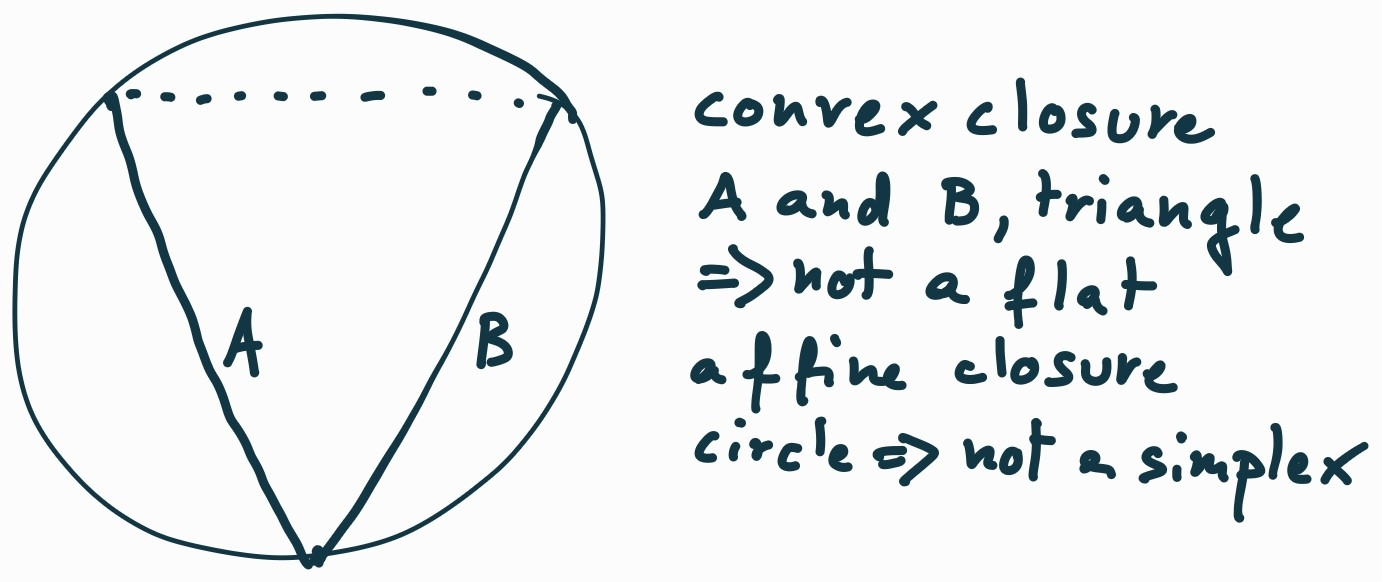
\includegraphics[width=0.75\textwidth]{tempimages/ContextClosureNotContext.jpg}
\end{figure}

\begin{remark}
	While a classical probability context can be decomposed into classical probability contexts whose closure is the original context, the converse is not true. That is, given two classical probability contexts, their convex or flat closure is not in general a classical probability context. Take a disk (the ensemble space) and two lines connecting three points (the two probability contexts). The convex closure is the triangle, which is not a flat as it misses some affine combinations. The flat closure is the disk, which is not a probability context.
\end{remark}

\begin{conj}
	Let $A, B \subseteq \Ens$ be two classical probability contexts. Then their flat closure and convex closure coincide if and only if these closures are a classical probability context.
\end{conj}

\begin{conj}
	The defining property of a classical probability context is exactly that property that allows $A$ and $B$ so constructed to be convex sets whose closure is $C$.
\end{conj}

\begin{prop}
	Let $C \subseteq \Ens$ be a classical probability context. Let $\mathfrak{L}$ be the lattice of $\separate$-subspaces. Then the fraction capacity is an additive set function on the lattice. That is, for all $\ens \in C$ and $A, B \in \mathfrak{L}$ such that $A \cap B = \emptyset$,  $\fcap_{\ens}(A \vee B) = \fcap_{\ens}(A) + \fcap_{\ens}(B)$.
\end{prop}

\begin{proof}
	Let $A, B\in \mathfrak{L}$ such that $A \cap B = \emptyset$. Then $A$ is separate from $B$. Therefore $A \vee B$ is a classical probability context that is the convex closure of two separate probability contexts. Therefore, as we saw in a previous proof, $A \vee B$ consists of convex combinations of $A$, which are all in $A$, of convex combinations of $B$, which are all in $B$, and of convex combinations of both, which are in neither $A$ nor $B$.
	
	We want to show that $\fcap_{\ens}(A \vee B) = \fcap_{\ens}(A) + \fcap_{\ens}(B)$ if $\ens \in A \vee B$. Let $\ens \in A \vee B$ be an ensemble that is the mixture of elements of $A$. Then $\ens \in A$ and it has no components in $B$. Therefore $\fcap_{\ens}(A \vee B) = 1$ and $\fcap_{\ens}(A) = 1$ while $\fcap_{\ens}(B) = 0$. This means $\fcap_{\ens}(A \vee B) = 1 = 1 + 0 = \fcap_{\ens}(A) + \fcap_{\ens}(B)$. If $\ens$ is a mixture of elements of $B$, we get the same conclusion. The last case is when $\ens$ is a mixture of elements of $A$ and $B$. That is, $\ens = \sum_i p_i \ens[a]_i + \sum_j \lambda_j \ens[b]_j$ with $\ens[a]_i \in A$, $\ens[b]_j \in B$, $p_i, \lambda_j \in [0,1]$ and $\sum_i p_i + \sum_j \lambda_j = 1$. By definition of fraction capacity, $\sum_i p_i \leq \fcap_{\ens}(A)$. Suppose $\sum_i p_i < \fcap_{\ens}(A)$. Then there is $\hat{\ens[a]} \in A$ such that $\ens = \sum_i p_i \ens[a]_i + p \hat{\ens[a]} + \lambda \ens[c]$ for some $p,\lambda \in [0,1]$ and $\ens[c] \in A \vee B$. But then $\ens$ would be separately multidecomposable, which is a contradiction since it is an element of a classical probability context. Therefore $\sum_i p_i = \fcap_{\ens}(A)$. Similarly, we find that $\sum_j \lambda_j = \fcap_{\ens}(B)$. Since $\sum_i p_i + \sum_j \lambda_j = 1$, $\fcap_{\ens}(A) + \fcap_{\ens}(B) = 1 = \fcap_{\ens}(A \vee B)$ for all $\ens \in A \vee B$.
	
	Now let $\ens \in C$. We have $(A \vee B)^\separate \in \mathfrak{L}$ and $(A \vee B) \cap (A \vee B)^\separate = \emptyset$. Therefore $\fcap_{\ens}(C) = \fcap_{\ens}(A \vee B)+ \fcap_{\ens}((A \vee B)^\separate)$. Note that $\ens$, in general, is a convex combination of elements of $A\vee B$ and $(A \vee B)^\separate$. Components in $A \vee B$ are convex combinations of elements of $A$ and $B$, which also disjoint. Therefore $\ens$ is a convex combination of elements of $A$, $B$ and $(A \vee B)^\separate$, which are pairwise disjoint. As before, since multidecomposability is forbidden in a classical probability context, the sum of the coefficients for each part will have to match the fraction capacity of its subcontext. Therefore $\fcap_{\ens}(A) +  \fcap_{\ens}(B) + \fcap_{\ens}((A \vee B)^\separate) = \fcap_{\ens}(C) = \fcap_{\ens}(A \vee B) + \fcap_{\ens}((A \vee B)^\separate)$. Thus $\fcap_{\ens}(A \vee B) = \fcap_{\ens}(A) +  \fcap_{\ens}(B)$ for all $\ens \in C$.
\end{proof}
\end{mathSection}

\subsection{Spectrum of a classical probability context}

To recover classical probability distributions, we need to recover the possible cases (i.e. the sample space) and the events (i.e. the $\sigma$-algebra) over which the probability distributions are defined. These are not necessarily states. For example, in the countinuous classical case, the sample space corresponds to the sets of possible values of position and momentum (i.e. the symplectic manifold over which the values are defined). In quantum mechanics, the sample space is the range of possible values defined by an observable (i.e. the spectrum of the operator). The goal here is to identify a single physically meaningful construction that will be able to work for all these cases.

Intuitively, while we cannot perfectly prepare a continuous variable, we can imagine making preparations that have narrower and narrower spread. For example, we can imagine a sequence of uniform distributions over $[-\frac{1}{i}, \frac{1}{i}]$. The spread will converge to the single value $0$, though the sequence of ensembles will not converge to an ensemble. Similarly, we can imagine a sequence of density matrices, or even wave-functions, for the quantum case. We will be able to characterize ensembles in terms of classical probability distributions over these limits, which represent merely a convenient tool for representation and calculation. That is, conceptually we are not starting from the sample space (i.e. the possible idealized values) and then constructing probability distributions on top; we start with a set of ensembles, which are the physical objects we are studying, and, in the case that satisfy particular properties, they can be represented as probability distributions over limits of sequences.

Mathematically, the construction uses the notion of subspaces defined in \ref{pm_es_subspaceSection} applied to separateness. We use separateness to constructs sets of ensembles that share the same support. These are the $\separate$-subspaces and are constructed by looking for pairs of sets such that all the elements of one are separate from all the elements of the other. These subspaces form a lattice: they have a partial order according to set inclusion. Therefore we can find sequences of subspaces that become more and more refined, whose elements have a narrower and narrower support. Using a standard technique in topology, the set of possible limits are identified by a collection of subspaces (called ultrafilters) that become smaller and smaller. These become the point of the spectra, the sample space.

Every subspace can then be understood as a set of limits, a set of ultrafilters, that are open sets in the topology of the spectra. The topology is the one generated by the those sets.

\begin{defn}
	Given a classical probability context $C \subseteq \Ens$, the \textbf{spectrum} $\sigma(C)$ is the set of equivalence classes of sequences of ensembles that eventually become separate from each other. More rigorously, given a probability context, the spectra is the collection of the ultrafilters of the lattice of $\separate$-subspaces $\mathfrak{L}^\separate(C)$. The spectrum of each $\separate$-subspace is given by $\sigma(A) \mapsto \{ x \in \sigma(C) \, | \, A \in x \}$. The standard topology of the spectrum is the one generated by the spectra of all $\separate$-subspaces (i.e. $\sigma(\mathfrak{L}^\separate(C))$.
\end{defn}

\begin{prop}
	Let $C \subseteq \Ens$ be a classical probability context and $\sigma(C)$ its spectrum. Then the following are true:
	\begin{enumerate}
		\item $A \subseteq B$ if and only if $\sigma(A) \subseteq \sigma(B)$
		\item $\exterior(\sigma(A)) = \sigma(A^{\separate})$
		\item $\partial \sigma(A) = \{ x \in \sigma(C) \, | \, A \notin x, A^{\separate} \notin x \}$
		\item $\sigma(A)^{\complement} = \overline{\sigma(A^{\separate})}$
		\item $\sigma(\bigwedge_{i \in I} A_i) = \interior\left(\bigcap_{i \in I} \sigma(A_i)\right)$
		\item $\sigma(\bigvee_{i \in I} A_i) = \interior\left(\overline{\bigcup_{i \in I} \sigma(A_i)}\right)$
		\item if $U$ open, then $U = \bigcup_{i \in I} \sigma(A_i)$ for some family of $A_i \in \mathfrak{L}^\separate(C)$
	\end{enumerate}
\end{prop}

\begin{proof}
	For 1, since all $x \in \sigma(C)$ are upward closed, $A \in x$ means $B \in x$ as well. Therefore if $x \in \sigma(A)$ then $x \in \sigma(B)$, which means $\sigma(A) \subseteq \sigma(B)$. Conversely, if $\sigma(A) \subseteq \sigma(B)$ then all downward sets of $\mathfrak{L}^\separate(C)$ that contain $A$ must also contain $B$, which means $B \supseteq A$.
	
	For 2 and 3, note that $\sigma(A) = \{ x \in \sigma(C) \, | \, A \in x \}$ and therefore $\sigma(A)^{\complement} = \{ x \in \sigma(C) \, | \, A \notin x \}$. Since $\sigma(A)$ is an open set, $\sigma(A)^{\complement} = \exterior(\sigma(A)) \cup \partial \sigma(A)$. Now consider $\sigma(A^{\separate})$. This is an open set and it is disjoint from $\sigma(A)$. In fact, if $x \in \sigma(A) \cap \sigma(A^{\separate})$ then $A, A^{\separate} \in x$. But this would mean that $\emptyset \in x$, which can't be because $x$ is a proper filter and cannot contain $\emptyset$. Since $A^{\separate}$ is the largest $\separate$-subspace that is separate from $A$, there is no set in $\sigma(\mathfrak{L}^\separate(C))$ that is larger than $A^{\separate}$ and still disjoint from $A$. Therefore $\sigma(A^{\separate}) = \exterior(\sigma(A))$. We have $\partial \sigma(A) = \sigma(C) \ (\interior(\sigma(A))\cup\exterior(\sigma(A))) = \{ x \in \sigma(C) \, | \, A \notin x, A^{\separate} \notin x \}$.
	
	For 4, since $\sigma(A)$ is an open set, the complement is the closure of the exterior. Therefore, given 1, $\sigma(A)^{\complement} = \overline{\sigma(A^{\separate})}$.
	
	For 5, consider $\bigwedge_{i \in I} A_i$. This is the largest $\separate$-subspace that is contained by all $A_i$. Then, given 1, $\sigma\left(\bigwedge_{i \in I} A_i\right)$ must be the largest open set that is contained by all $\sigma(A_i)$. This corresponds to $\interior\left(\bigcap_{i \in I} \sigma(A_i)\right)$.
	
	For 6, we have
	\begin{align*}
		\sigma(\bigvee_{i \in I} A_i) &= \exterior(\exterior(\sigma(\bigvee_{i \in I} A_i))) = \exterior(\sigma((\bigvee_{i \in I} A_i)^{\separate})) = \exterior(\sigma(\bigwedge_{i \in I} A_i^{\separate})) \\
		&= \exterior(\interior(\bigcap_{i \in I} \sigma(A_i^{\separate}))) = \exterior(\bigcap_{i \in I} \sigma(A_i^{\separate})) =  \\
		&= \exterior\left(\bigcap_{i \in I}\overline{\sigma(A_i)}^{\complement}\right) = \exterior\left(\left(\bigcup_{i \in I}\overline{\sigma(A_i)}\right)^{\complement}\right) \\
		&= \interior\left(\bigcup_{i \in I}\overline{\sigma(A_i)}\right)
	\end{align*}
	For the last step, not that the union of the closure is not necessarily the closure of the union, but they have the same interior.
	
	For 7, note that an open set $U$ is generated from $\sigma(\mathfrak{L}^\separate(C))$ through finite intersection and arbitrary union. Note that the finite intersection, of open sets is an open set, so we have $\bigcap_{i \in I} \sigma(A_i) = \interior\left(\bigcap_{i \in I} \sigma(A_i)\right) = \sigma(\bigwedge_{i \in I} A_i)$. Therefore the finite intersection corresponds to a $\separate$-subspace. This means that we can can generate all open sets with arbitrary unions of sets from $\sigma(\mathfrak{L}^\separate(C))$.
\end{proof}

\begin{remark}
	Note that while the lattice of the $\separate$-subspaces is a topped intersection structure, the lattice of the corresponding closed sets is not. The intersection of the $\separate$-subspaces corresponds to the interior of the intersection of their spectra. A point of the spectra, in fact, can correspond to an infinitesimal subspace (i.e. a non-principal/free ultrafilter) which corresponds to no actual ensemble.
	
	As an example, suppose we are taking the lattice of probability measures defined over the interval $[0,1]$ that are absolutely continuous with respect to the Lebesgue measure. Each $\separate$-subspace will correspond to a set of measures whose support lives in a particular region. A singleton will not correspond to any subspace as it cannot support an absolutely continuous measure. Therefore, if we take all the $\separate$-subspaces of all measures that have $1/2$ within the support, the intersection of all those subspaces will be the empty set, which is a $\separate$-subspace. However, the intersection of the sets representing their support is the singleton $\{1/2\}$, which is not the empty set. However, its interior is the empty set.
	
	The fact a single probability measure is an equivalence class of probability densities is related to this distinction. Consider a uniform distribution over $[0,1]$. The related probability density can be understood as a constant between those values and zero everywhere else. However, the same constant over $[0,1/2) \cup (1/2,1]$ will also work. That is, the same element of the ensemble space can be represented in different way as a function over the spectra.
\end{remark}


\begin{thrm}
	Let $C \subseteq \Ens$ be a probability context and $\ens \in C$ be an ensemble in the context. The set function $p^*_{\ens} : \textsf{T}_{\sigma(C)} \to[0,1]$, defined such that $p^*_{\ens}(U) = \inf(\{ \fcap(A) \, | \, \sigma(A) \supseteq U \})$, is a topological measure. Therefore ensemble in a classical probability context can be represented by a unique measure over its spectra that is continuous with respect to its topology.
\end{thrm}

\begin{proof}
	Since $p^*_{\ens}$ is finite, it is locally finite. We need to show that is topologically additive. If $U$ is a generic open set, then we are looking for the smallest subspace $A$ such that $\sigma(A) \subseteq U$. If $U$ corresponds to a $\separate$-subspace, that is $U = \sigma(A)$, then $p^*_{\ens} = \fcap_{\ens}(A)$. If not, $U$ can still be written as the union of the spectrum of a family of subspaces. That is, $U = \bigcup_{i \in I} \sigma(A_i)$ for some family of $A_i \in \mathfrak{L}^\separate(C)$. The smallest subspaces that contains them all, then is the join $A$. Therefore we have $p^*_{\ens}(U) = p^*_{\ens}(\sigma(A)) = p^*_{\ens}(\sigma(\bigvee_{i \in I} A_i)) = p^*_{\ens}\left(\interior\left(\overline{\bigcup_{i \in I} \sigma(A_i)}\right)\right)$. Lastly, let $U_i$ be a family of disjoint open sets and let $A_i$ be the corresponding smallest subspaces such that $\sigma(A_i) \supseteq U_i$. Since $U_i$ are disjoint, $A_i$ will also be disjoint, and therefore they will be separate. But the fraction capacity is additive across separate subspaces. We have $\sum_{i \in I} p^*_{\ens}(U_i) = \sum_{i \in I} \fcap_{\ens}(A_i) = \fcap_{\ens}(\bigvee_{i \in I} A_i) = p^*_{\ens}\left(\interior\left(\overline{\bigcup_{i \in I} \sigma(A_i)}\right)\right) = p^*_{\ens}\left(\interior\left(\overline{\bigcup_{i \in I} U_i}\right)\right)$. Therefore $p^*_{\ens}$ is a topological measure.
	
	The measure, then, can be extended uniquely to the whole $\sigma$-algebra, since the measure is finite.
	
	Lastly, we need to show that two different ensembles will correspond to two different measures. Let $\ens[a],\ens[b] \in C$ be two distinct ensembles in the probability context. TODO
\end{proof}

\begin{conj}
	A convex subset $U \subset \Ens$ is a classical probability context if and only if it is the subset of probability measures of a vector space of measures over a sample space $\Omega$.
\end{conj}

\begin{prop}
	Let $\Ens$ be a discrete classical ensemble space. Then $\Ens$ is a probability context, the spectra is the sample space and its topology is the discrete topology.
\end{prop}

\begin{proof}
	Let $\Ens$ be a discrete classical ensemble space. The whole space is a flat as it contains all its affine combinations. Note that two ensembles are separate if and only if they have disjoint support. Suppose $\ens = p \ens[a]_1 + \bar{p} \ens[a]_2 = \lambda \ens[b]_1 + \bar{\lambda} \ens[b]_2$. Then the union of the support of each pair must be the same. Therefore the support at least one element of each pair must overlap with the support of another element of another pair. This means that separate multidecomposability is not allowed. Therefore $\Ens$ is a classical probability context.
	
	Since ensembles are separate if and only if they have disjoint support, the $\separate$-closure of a subset $A \subseteq \Ens$ of ensembles corresponds to all ensembles whose support is a subset of the union of the supports of the elements of $A$. Each $\separate$-subspace, then, is associated to one unique subset $U \subseteq \Omega$ of the sample space. Given that for any subset $U$ we can find a measure whose support is $U$, every subset corresponds a unique $\separate$-subspace. If the support of a measure is a subset of $U$, it will also be a subset of any other set $V \supseteq U$. Therefore the ordering of the lattice of $\separate$-subspaces is the same as inclusion on the lattice of supports. The two lattices are isomorphic.
	
	Since the singletons are elements of the lattice, all ultrafilters are principal, meaning that they are all of the form $X(x) = \{A \in \mathfrak{L}^\separate(C) \, | \, \{x\} \in A\}$ where $x \in \Omega$ is an element of the sample space. Therefore the sample space and the spectra coincide. Each singleton is a closed set, since it is an element of the lattice. The complement of each singleton is also an element of the lattice, therefore each singleton is also an open set. The topology is therefore the discrete topology.
\end{proof}

\begin{remark}
	TODO: organize. There are different types of limits. One limit of convex combinations. Physically, these are mixtures over infinitely many elements. Limit of ensemble sequences. Physically, these are sequences of ensembles, taken one after the other, for example in temporal succession. Limits of ensembles taken from $\separate$-subspaces strictly included into each other. This is the limit of ensemble that are finer and finer.
\end{remark}

\subsection{Classical probability contexts in classical and quantum ensemble spaces}

We now want to show the relationship between classical probability context for classical and quantum ensembles spaces. For classical ensemble spaces the connection is simple: every classical ensemble space is classical probability context. The reverse is not true. We could have, for example, an ensemble space that is exactly like the discrete classical one except for the entropy of the pure states, which are all assumed to be zero in a discrete classical ensemble space. The convex space structure would be exactly the same, but the entropy wouldn't match. We could also have a space of probability functions defined on a space that is not symplectic. This would be classical probability contexts, but not a space of classical ensembles.

\begin{conj}
	Discrete and continuous classical ensemble spaces are classical probability contexts.
\end{conj}

%\begin{proof}
%	Let $\Ens$ be a classical probability space and let $\mu, \nu \in \Ens$ be probability measures on some space $\Omega$. The space of probability measures is a subset of the space of signed measures. This space can be equipped with an inner product. The space of signed measures with support $U \subseteq \Omega$ forms a subspace. This means that, if we can find a $U \subseteq \Omega$ such that both $\mu(U) \neq 0$ and $\nu(U) \neq 0$, we can find a probability measure that is a component of both. That is, two probability measures that have overlapping support have a common component. Conversely, given that convex combination can only expand the support of measures, two probability measures that have no overlapping support have no common components. (TODO: if all measure are allowed, we may get also measures we do not want - Dirac measures, measures that have no continuous derivative. If not all measures are allowed, we have no existence of a measure that can be a component, and therefore there may be overlapping measures that have no common components.)
	
%	Now, suppose $\ens \separate \ens[a]$ and $\ens \separate \ens[b]$. This means that the support of $\ens$ is disjoint from the support of both $\ens[a]$ and $\ens[b]$, which will also be disjoint from the support of any mixture of $\ens[a]$ and $\ens[b]$ since the support of the mixture will be the union of the individual supports. This means that $\ens$ will be separate from all mixtures of $\ens[a]$ and $\ens[b]$. The property holds, then, in any classical ensemble space.
%\end{proof}

A quantum ensemble space, however, does not allow a description in terms of classical probability precisely because it allows separate multidecompositions.

\begin{prop}
	A quantum ensemble space is not a classical probability context.
\end{prop}

\begin{proof}
Let $\Ens$ be a quantum ensemble space. Let $A \subseteq \Ens$ the space of mixtures of a two dimensional subspace (i.e. a Bloch sphere) and consider the states $x^+$, $x^-$, $z^+$, and $z^-$, which are points on the surface that form a square. These are all separate ensembles. We have $\frac{1}{2} x^+ + \frac{1}{2} x^- = \frac{1}{2} z^+ + \frac{1}{2} z^-$ therefore the space allows separate multidecomposition and is not a classical probability context.
\end{proof}

However, given a maximal set of commuting observables, we can define a classical probability context as the set of all mixed states that commute with all the observables. This makes the spectrum of all the density operator coincide with the product of the spectra of all commuting observables, and therefore those mixed states can be characterized by a measure over the spectra.

\begin{conj}
	Let $\Ens$ be a quantum ensemble space. Let $O_i$ a maximal set of commuting observables. Let $C \subseteq \Ens$ be the set of mixed state that commute with all $O_i$. Then $C$ is a classical probability context.
\end{conj}

\section{Statistical properties and quantities}

TODO: from here on are just old notes to be reorganized

\subsection{Maximal component sequence}

\begin{defn}
	Let $\ens \in \Ens$ be an ensemble. A sequence of ensembles $\{\ens[a]_i\} \subseteq \Ens$ is an \textbf{increasing component sequence of $\ens$} if we can write
	\begin{align*}
		\ens &= p_i \ens[a]_i + \bar{p}_i \ens[b]_i  \\
		\ens[a]_{i+1} &= \frac{p_i}{p_{i+1}} \ens[a]_i + \frac{p_{i+1} - p_i}{p_{i+1}} \Delta \ens[a]_i
	\end{align*}
	where $\{\ens[b]_i\} \subseteq \Ens$, $\{\Delta\ens[a]_i\} \subseteq \Ens$ and $\{p_i\} \subseteq (0,1]$ is an increasing sequence. The \textbf{fraction} of the sequence is the limit $p_i \to p$.
\end{defn}

\begin{remark}
	Since the sequence of $p_i$ is increasing and is bounded, it must converge. The set of all possible limits is bounded and therefore must have a supremum.
\end{remark}

\begin{defn}
	Let $\ens \in \Ens$ be an ensemble and $A \subseteq \Ens$ a set of ensembles. Then the \textbf{$A$-components of $\ens$} are the components of $\ens$ that are mixtures of $A$. That is, $A_{\ens} = \{ \ens_1 \in \hull(A) \, | \, \exists p \in (0,1], \ens_2 \in \Ens \text{ s.t. } \ens = p \ens_1 + \bar{p} \ens_2  \}$. An \textbf{increasing $A$-component sequence of $\ens$} is an increasing component sequence of $\ens$ such that $\{\ens[a]_i\} \subseteq \hull(A)$ and $\{\Delta\ens[a]_i\} \subseteq \hull(A)$. The sequence $\{\ens[a]_i\} \subseteq \hull(A)$ is \textbf{maximal} if the fraction of the sequence is $\fcap_{\ens}(A)$.
\end{defn}

\begin{coro}
	The fraction of $A$-component sequences are bounded by $\fcap_{\ens}(A)$.
\end{coro}

\begin{proof}
	For all elements of component sequences we have $p_i \leq \fcap_{\ens}(A)$. Therefore the limit of $p_i$ cannot exceed $\fcap_{\ens}(A)$.
\end{proof}

\begin{prop}
	Let $\ens \in \Ens$ be an ensemble and $A \subseteq \Ens$ a set of ensembles, then there exists a maximal $A$-component sequence of $\ens$.
\end{prop}

\begin{proof}
	Consider the hull of $A$. This can be ordered by the fraction $\size_{\ens}$, which is less or equal to one. If there is a maximum, then simply take a sequence of an element with the maximum faction. If not, we can take a sequence of ever increasing fractions whose limit is the fraction capacity, and find a corresponding sequence of ensembles within $\hull(A)$. By definition, this will be a maximal $A$-component sequence of $\ens$.
\end{proof}

\begin{prop}
	Let $\{\ens[a]_i\} \subseteq \hull(A)$ be an $A$-component sequence of $\ens \in \Ens$. A \textbf{complement} sequence is an increasing sequence $\{\ens[b]_i\} \subseteq \Ens$ such that
	$$ \ens = p_i \ens[a]_i + q_i \ens[b]_i + \overline{(p_i + q_i)} \ens[\epsilon]_i $$
	where $\{\ens[\epsilon]_i\} \in \Ens$ and $(p_i + q_i) \to 1$. In this sense, the sum of the two sequences converges to $\ens$.
\end{prop}

\begin{remark}
	Note that complement sequences always exist since we can set $\ens[\epsilon]_i = \ens[b]_i$, $q_i = \bar{p}$ and recover the definition of a component sequence.
\end{remark}

\begin{prop}
	An $A$-component sequence $\{\ens[a]_i\} \subseteq \hull(A)$ of $\ens \in \Ens$ is maximal if and only if it admits a complement sequence that is always separate from the hull of A. That is, $\{\ens[b]_i\} \separate \hull(A)$.
\end{prop}

\begin{proof}
	Suppose that $\{\ens[a]_i\}$ is maximal and let $\{\ens[b]_i\}$ be a complement.
	$$ \ens = p_i \ens[a]_i + q_i \ens[b]_i + \overline{(p_i + q_i)} \ens[\epsilon]_i.$$
	
\end{proof}

\begin{prop}
	Let $\ens \in \Ens$ be an ensemble, $A \subseteq \Ens$ a set of ensembles and $\ens[a]_i$ and $\ens[b]_i$ two maximal $A$-component sequence of $\ens$. Then we can write $\ens[a]_i = p_i \ens[b]_i + \bar{p}_i \ens[c]_i$ where $\ens[c]_i \in \Ens$, $p_i \in [0,1]$ and $p_i \to 1$.
\end{prop}

\begin{proof}
	Note that we can always write $\ens[a]_i = p_i \ens[b]_i + \bar{p}_i \ens[c]_i$ because we can always choose $p_i = 0$ and $\ens[c]_i = \ens[a]_i$. Therefore, if the proposition is not true, we can always find $p_i \to p$, except that $p \neq 1$.
	
	Suppose the proposition is not true. We can still write $\ens = \lambda_i \ens[a]_i + \bar{\lambda}_i \ens[d]_i = \lambda_i p_i \ens[b]_i + \lambda_i \bar{p}_i \ens[c]_i + \bar{\lambda}_i \ens[d]_i$. But $\ens[b]_i$ is maximal, therefore $\lambda_i p_i \ens[b]_i$ can be increased. But $\ens[c]_i \in \hull(A)$, which means we can write an $A$-component sequence whose fraction is higher than the maximal, which cannot be. Therefore the proposition is true.
	
	TODO: this may need to be fixed. Can't reconstruct the argument.
\end{proof}

\subsection{Statistical properties}

In the same way that we define ensembles first, we define quantities through their expectation over ensembles. The possible value for pure states will need to be recovered with constructions that are connected to spectral theory.

\begin{defn}
	A \textbf{statistical property}, or simply property, is an attribute that allows statistical handling. Formally, it is a continuous map $F : \Ens \to \mathcal{Q}$ where $\mathcal{Q}$ is a convex topological space such that $F(p \ens_1 + \bar{p} \ens_2) = p F(\ens_1) + \bar{p} F(\ens_2)$.
	
	A \textbf{statistical quantity}, or statistical variable, or simply variable, is a numerical statistical property. That is, it is a continuous linear real valued operator $F : \Ens \to \mathbb{R}$.
\end{defn}

\begin{justification}
	This definition extends the general definition of properties and quantities we already gave to the statistical case. As before, continuity is required since verifying the value of the quantity corresponds to verifying that we are dealing with a specific subset of ensembles.
	
	The ability to create convex combinations corresponds to the ability to create statistical averages. Therefore $\mathcal{Q}$ must be a convex set. Given that preparations are assumed to be independent, the a mixture of the preparation will produce a mixture of the properties according to the same fractions. 
	
	Quantities are simply properties that are linearly ordered. The ability to create convex combinations becomes the ability to take weighted averages of the quantities. Regardless of whether one starts from integers, rationals or real valued quantities, the statistical averages will, in general, be a real number.
	
	Note that the numerical value cannot be infinite. The only way to measure infinity is if the measured average keeps increasing in time. This would be a contradiction on the assumption that the ensemble is reproducible.
\end{justification}

\begin{remark}
	Note that variables will have a contiguous range on the ensembles because, given two ensembles with different values, we can mix them to obtain any intermediate value. This does not mean that the variable can take all possible values on pure states. For example, the number of particles in a pure state will necessarily be a non-negative integer, but we can mix those to create ensembles that have non-integer average number of particles.
\end{remark}

\begin{coro}
	A set of statistical quantities $\{F_i\}_{i \in I}$ can be collected into a single statistical property $F : \Ens \to \mathbb{R}^I$ where $F(\ens) = \{F_i(\ens)\}_{i \in I}$.
\end{coro}

\begin{prop}
	Let $\Ens$ be a classical probability space. Then each statistical quantity is the expectation of a random variable and vice-versa.
\end{prop}

\begin{proof}
	Let $\Ens$ be an ensemble space where each ensemble is a probability measure $\mu$ over some sample space $\Omega$. Let $f : \Omega \to \mathbb{R}$ be a random variable, then the expectation $F(\mu) = \int_{\Omega} f d\mu$ is a statistical quantity. Conversely, let $F : \Ens \to \mathbb{R}$ be a linear functional of the measures. Then, by (TODO: CHECK) Riesz representation theorem, we can write $F(\mu) = \int_{\Omega} f d\mu$ from some $f : \Omega \to \mathbb{R}$.
\end{proof}

\begin{conj}
	Let $\Ens$ be a quantum ensemble space. Then each statistical quantity is the expectation of an observable and vice-versa.
\end{conj}

\begin{proof}
	TODO: need to find a quantum correspondent of the Riesz representation theorem.
\end{proof}

\begin{conj}
	Let $e \in \Ens$ be an ensemble, $F : \Ens \to \mathbb{R}$ be a statistical variable and $A \subset \Ens$ be a set of ensemble. Let $\ens[a]_i$ and $\ens[b]_i$ be maximal $A$-component sequences of $\ens$. Then $\lim_{i \to \infty} F(\ens[a]_i) = \lim_{i \to \infty} F(\ens[b]_i)$.
\end{conj}

\begin{defn}
	Let $e \in \Ens$ be an ensemble, $F : \Ens \to \mathbb{R}$ be a statistical variable and $A \subset \Ens$ be a set of ensemble. Then the \textbf{contribution to $F$ over $A$ given $\ens$} is the limit of variable for a maximal $A$-component sequence of $\ens$. That is, $F_{\ens}(A) = \lim_{i \to \infty} F(\ens[a]_i)$ where $\ens[a]_i$ is a maximal $A$-component sequence of $\ens$.
\end{defn}

\begin{prop}
	The contribution to $F$ is a set function.
\end{prop}

\begin{proof}
	Since $F_{\ens}$ takes a set of an argument and returns a real value, is a set function.
\end{proof}

\begin{remark}
	Note that the contribution cannot be monotone in the same way that the expectation of a random variable to an event is not monotone. Not clear whether the additivity of the variable may tell us something about the additivity of the contribution.
\end{remark}

\begin{conj}
	We can define a ``derivative'' $f_{\ens}$ between $F_{\ens}$ and $\fcap_{\ens}$ such that $F_{\ens}(A) = \int_A f_{\ens} \, d \fcap_{\ens}$ where $\int$ is the ??? integral.
\end{conj}

\begin{remark}
	This may still not be the correct formulation of the problem. Note that $A$ is a set of ensembles. In the classical case it would correspond to a set of probability measures, not a subset of the sample space (i.e. an event). However, in the discrete case and in the quantum case, $A$ can also be restricted to a set of pure state (i.e. extreme points), which would correspond to a subset of the sample space. It may be worth at least understanding that case.
\end{remark}

\subsection{Quantifiable spaces and locally convex vector spaces}

\begin{prop}
	Let $\Ens$ be a complemented ensemble space. Then a statistical variable $F$ induces a semi-norm on the vector space that embeds $\Ens$.
\end{prop}

\begin{proof}
	Let $F$ be a variable on $\Ens$ and let $V$ be the vector space that embeds $\Ens$. Extend $F$ on $V$ such that $F(a\ens) = |a| F(\ens)$. Then, according to the definition given after 1.1 in \url{https://personal.math.ubc.ca/~cass/research/pdf/TVS.pdf} $F$ is a semi-norm.
\end{proof}

\begin{defn}
	A \textbf{quantifiable} ensemble space is an ensemble space where each ensemble can be identified by a set of statistical variables. That is, there is family of statistical variables $F_i : \Ens \to \mathbb{R}$ such that, given $\ens_1, \ens_2 \in \Ens$, $F_i(\ens_1) = F_i(\ens_2)$ for all $i$ if and only if $\ens_1 = \ens_2$. Moreover, the topology is generated by those variables.
\end{defn}

\begin{prop}
	A quantifiable ensemble space is complemented and embeds into a Hausdorff locally convex topological vector space.
\end{prop}

\begin{proof}
	Let $\ens[a], \ens[b], \ens[c] \in \Ens$ be three ensembles such that $p \ens[a] + \bar{p} \ens[b] = p \ens[a] + \bar{p} \ens[c]$ for some $p \in (0,1)$. For any statistical variable $F : \Ens \to \mathbb{R}$ we have
	\begin{equation}
		\begin{aligned}
			F(p \ens[a] + \bar{p} \ens[b]) &= F(p \ens[a] + \bar{p} \ens[c]) = p F(\ens[a]) + \bar{p} F(\ens[b]) = p F(\ens[a]) + \bar{p} F(\ens[c])\\
			F(\ens[b]) &= F(\ens[c]) 
		\end{aligned}
	\end{equation}
	For a quantifiable ensemble space with statistical variables $F_i$, we have $F_i(\ens[b]) = F_i(\ens[c])$, which means $\ens[b] = \ens[c]$. Since $\ens[a]$, $\ens[b]$, $\ens[c]$ and $p$ where arbitrary, the space is complemented.
	
	The ensemble is complemented, therefore it is embedded into a vector space. The topology of the ensemble space is generated by the statistical variables, which induce semi-norms on the vector space. This means that the topology of the vector space is generated by a countable set of semi-norms, and is therefore a locally convex topological vector space. See Prop 2.2 in \url{https://personal.math.ubc.ca/~cass/research/pdf/TVS.pdf}.
	
	The statistical variables fully identify each ensemble, which means that, if two elements are different, one semi-norm will give a non-zero value for the distance function associated with it. This means that the topology is Hausdorff. See Prop 2.6 in \url{https://personal.math.ubc.ca/~cass/research/pdf/TVS.pdf}.
\end{proof}

\begin{coro}
	A quantifiable ensemble spaces is fully determined by countably many statistical variables.
\end{coro}

\begin{proof}
	The topology of an ensemble space is second countable. A Hausdorff second countable locally convex topological vector space can always be generated by countably many semi-norms.
\end{proof}

\begin{remark}
	Note that we are missing completeness in terms of the semi-norms to obtain a Fr\'echet space. It is not clear whether this is required since, for example, $L^1(\mathbb{R}^{2n}) \cap C(\mathbb{R}^{2n})$ is not Fr\'echet.
\end{remark}

\begin{conj}
	Discrete/continuous classical ensemble spaces and quantum ensemble spaces are quantifiable.
\end{conj}

\begin{proof}
	For discrete classical spaces, the expectation of the indicator of each extreme point defines a countable set of quantities that fully identifies the distribution.
	
	For continuous classical spaces, $L^1(\mathbb{R}^{2n}) \cap C(\mathbb{R}^{2n})$ is a Hausdorff locally convex topological spaces.
	
	TODO Quantum (note that we are looking at the space of density operators with finite expectation value for position and momentum).
\end{proof}

\begin{conj}
	If all ensembles can be connected by linear transformations parameterized by real quantities, then the ensemble is quantifiable.
\end{conj}

\begin{remark}
	Note clear whether this is true. The idea is that the time interval can be used to define variables. A more sophisticated conjecture may look at the space of generators of Lie groups. This would link the topology of time to the topology of the ensemble space. If the topology of time is not that of the real numbers, then, the ensemble space must change significantly.
\end{remark}

% TODO: for later
%\begin{conj}
%	Let $\ens \in \Ens$ and $A \subset \Ens$. Let $\{\ens[a]_i\}$ and $\{\ens[b]_i\}$ be two maximal increasing $A$-component sequence. Then $\lim\limits_{i \to \infty} F(\ens[a]_i) = \lim\limits_{i \to \infty} F(\ens[a]_i)$ for any quantities $F$.
%\end{conj}

\begin{proof}
	Check that the all maximal sequences give the same value.
\end{proof}

\subsection{Macrostates and thermodynamics}

TODO: This should be moved after the definition of entropy.

In this section we try to recover some elements of thermodynamics on the generalized ensemble space. We want to recover Gibbs' thermodynamics, which means an equation of state in terms of extensive quantities. Instead of extensive quantities, we are going to use statistical quantities. Note that the idea that all extensive quantities are statistical (i.e. the average during mixing) seems to work. The energy and the number or particles average during mixture. The idea that volume averages during mixture can be understood as the system oscillating between the different volumes defined by the components. It also seems that intensive quantities do not average during mixing. Temperature, for example, is only defined on equilibria (i.e. of Boltzmann distributions) and the mixture of two equilibria at different temperature is not an equilibrium. Still, we would need a general proof, which would require the notion of product spaces (i.e. intensitive/extensive quantities represent system/subsystem relationship).

\begin{defn}
	Let $\Ens$ be an ensemble space. Let $F : \Ens \to \mathcal{Q}$ be a statistical property. The \textbf{coarse graining} of $\Ens$ over $F$ is the set $\mathcal{M} \subseteq \Ens$ represented by the ensemble that maximize the entropy for each fixed value of the property. That is, there exists a map $\psi : \mathcal{Q} \to \mathcal{M}$ such that $F(\psi(x)) = x$ and $S(\psi(x)) \geq \ens$ for all $\ens \in \Ens$ such that $F(\ens) = x$. The \textbf{equation of state} is the map $S(x) \mapsto S(\psi(x))$ that returns the entropy given the value of the statistical property.
\end{defn}

\begin{conj}
	Let $F : \Ens \to \mathbb{R}^n$ be a vector of statistical quantities. Then the corresponding coarse graining of $\mathcal{M}$ is a manifold. The equation of state $S : \mathbb{R}^n \to \mathbb{R}$ returns the entropy as a function of the statistical values.
\end{conj}

\begin{remark}
	We need to prove that $\mathcal{M}$ inherits the topology from $\Ens$. Are we be able to recover the topological isolation of phase transitions? The quantities will typically be energy plus other extensive quantities (i.e. volume, number of particles, ...).
\end{remark}

\begin{prop}
	The equation of state is strictly concave. That is, $S(\lambda x + \bar{\lambda} y) \geq \lambda S(x) + \bar{\lambda} S(y)$ and the equality holds if and only if $x=y$.
\end{prop}

\begin{proof}
	Let $x, y \in \mathcal{Q}$ be two possible values for the statistical property, and let $\lambda x + \bar{\lambda} y$ be a convex combination. We have $F(\psi(\lambda x + \bar{\lambda} y)) = \lambda x + \bar{\lambda} y = F(\lambda \psi(x) + \bar{\lambda} \psi(y))$. That is, $\psi(\lambda x + \bar{\lambda} y)$ and $\lambda \psi(x) + \bar{\lambda} \psi(y)$ are two ensembles that share the same value for the statistical property. By definition, the entropy of the first cannot be lower than the entropy of the second. We have
	\begin{equation}
		\begin{aligned}
			S(\lambda x + \bar{\lambda} y) &= S(\psi(\lambda x + \bar{\lambda} y)) \\
			&\geq S(\lambda \psi(x) + \bar{\lambda} \psi(y)) \\
			&\geq \lambda S(\psi(x)) + \bar{\lambda} S(\psi(y)) \\
			&= \lambda S(x) + \bar{\lambda} S(y),
		\end{aligned}
	\end{equation}
	which shows that the equation of state is concave.
	
	Now suppose that $x=y$. Then on one side $S(\lambda x + \bar{\lambda} y) = S(x)$ and on the other side $\lambda S(x) + \bar{\lambda} S(y) = S(x)$. $S(\lambda x + \bar{\lambda} y) = \lambda S(x) + \bar{\lambda} S(y)$. Conversely, suppose that $x\neq y$. Then $\psi(x) \neq \psi(y)$. By the strict concavity of the entropy, we have
	\begin{equation}
		\begin{aligned}
			S(\lambda x + \bar{\lambda} y) &= S(\psi(\lambda x + \bar{\lambda} y)) \\
			&\geq S(\lambda \psi(x) + \bar{\lambda} \psi(y)) \\
			&> \lambda S(\psi(x)) + \bar{\lambda} S(\psi(y)) \\
			&= \lambda S(x) + \bar{\lambda} S(y),
		\end{aligned}
	\end{equation}
	which shows that the equation of state is strictly concave.
\end{proof}

\begin{remark}
	In the case of thermodynamics, where the statistical property is a vector of statistical values, the equation of state will be concave in all arguments and in all combination of arguments.
\end{remark}


\subsection{Spectra of a quantity}

This is an attempt to define spectra purely on the topology and the convex structure, without reference to entropy and therefore inner product structure. It is unclear whether this is possible. If it is not possible, this attempt is still useful to understand what are the required definitions.

\begin{defn}
	Let $\Ens$ be an ensemble space and let $F : \Ens \to \mathbb{R}$ be a statistical quantity. Let $U \subset \mathbb{R}$ an open set of possible values for the quantity. We define the set of \textbf{ensembles supported by $U$} as the convex set $A \subset \Ens$ such that for any component $\ens$ of any element $\ens[a] \in A$ $F(\ens) \in U$. That is, they are all the elements that can be mixed among each other and still have all components have an expectation that fall within $U$.
\end{defn}

\begin{remark}
	Note that even if we have $F(\ens) \in U$ for some $\ens$, we can still have that no ensemble is supported by $U$. Consider a simply two dimensional discrete classical space $p\ens[a] + \bar{p} \ens[b]$ with $F(\ens[a]) = 0$ and $F(\ens[b]) = 1$. Now consider $U = \left(\frac{1}{4}, \frac{3}{4} \right)$. Ensembles for which $F(\ens) \in U$ are necessarily mixtures of $\ens[a]$ and $\ens[b]$, and $F(\ens[a])\neq 0 \neq F(\ens[b])$. Therefore no ensemble is supported by $U$.
	
	On the other hand, even if we have ensembles for which the expectation for all the components falls in $U$, they may still not be supported by $U$. Consider a Bloch ball for a qubit and  $F : \Ens \to \mathbb{R}$ such that $F(|0\>\<0|) = 0$ and $F(|1\>\<1|) = 1$. We have $F(|+\>\<+|) = F(|-\>\<-|) = \frac{1}{2}$ and therefore any mixture of those states
\end{remark}

\begin{defn}
	Given a statistical quantity $F : \Ens \to \mathbb{R}$, its \textbf{spectrum} $\sigma(F) \subseteq \mathbb{R}$ is the set of values $f \in \mathbb{R}$, called \textbf{spectral elements}, such that the set of ensembles supported by an open set that contains $f$ is non-empty.
\end{defn}

\begin{prop}
	
\end{prop}

\begin{conj}
	We recover an equivalent notion of spectra for both classical and quantum mechanics.
\end{conj}

Note that, in principle, the definitions only use $\mathbb{R}$ as a topological space (that also has a convex structure). Maybe this can generalize in the case that quantities are not real numbers.

\section{Reducibility}

\subsection{Reducible ensemble spaces}

\begin{defn}
	An ensemble space $\Ens$ is \textbf{reducible} if separate ensembles are also orthogonal. That is, $\ens_1 \separate \ens_2$ implies $\ens_1 \ortho \ens_2$.
\end{defn}

\begin{justification}
	Given that $\ens_1 \ortho \ens_2$ implies $\ens_1 \separate \ens_2$, classical spaces add the opposite implication. Therefore they exclude the case where two ensembles are orthogonal but not separate. This case describes two ensembles that have elements in common, but there is no ensemble corresponding to those common elements. That is, we cannot refine the ensembles into three separate ones: one with only elements of the first, one with only elements of the second and one with elements of both. In other words, we cannot reduce the coarser description of the system into finer separate descriptions. In the excluded case, then, the coarser description is irreducible into finer ensembles. This justifies the definition.
	
	As we prove below, that case does not exist in classical mechanics, but exists in quantum mechanics. This justifies calling the property classical.
\end{justification}

\begin{prop}
	Continuous and discrete classical ensemble spaces are reducible.
\end{prop}

\begin{proof}
	In both cases, ensembles are probability measures: the first over the Borel algebra of a symplectic manifold; the second over the power set of countably many elements. In both cases, the upper bound of the entropy is maximized if and only if the probability measures being combined have disjoint support. This means that two ensembles are orthogonal if and only if the respective probability measures have disjoint support. Intuitively, two probability distributions can have a common sub-distribution if and only if they overlap. Therefore two ensembles representing probability measures with disjoint support are exactly ensembles that are separate. Therefore, in both cases, the ensemble space is reducible.
\end{proof}

\begin{conj}
	An ensembles space is reducible only if it is classical.
\end{conj}

\begin{remark}
	The reverse direction cannot, in general, work. Take the subspace of a finite classical discrete ensemble space such the maximum probability of any element is $k < 1$. This corresponds to a simplex of the same dimension, with the same center, but scaled in the interior. Given that it is a convex subset of an ensemble space, it will satisfy all the axioms, except it will contain no orthogonal ensembles. Yet, it contains separate ensembles, which cannot be orthogonal.
\end{remark}

\section{R-subspaces}\label{pm_es_subspaceSection}

Here we present a generic construction that we will be using in a couple of different ways to construct lattice of subspaces. The general idea can be understood by looking at vector spaces with an inner product. The inner product defines a notion of orthogonality between vectors and this notion of orthogonality can be used to construct subspaces in the following way. If we take a set $U \subseteq V$ of vectors, we can define the set $U^{\perp}$ of all the vectors that are orthogonal to all elements of $U$. This will return the subspace orthogonal to all elements of $U$. We can also define $(U^{\perp})^{\perp}$ as the set of all the vectors that are orthogonal to all elements of $U^{\perp}$. The set $(U^{\perp})^{\perp}$ will contain all the elements of $U$, because they are all perpendicular to all elements of $U^{\perp}$ by definition, but it will also include all the elements in the same subspace. If $U$ were a subspace to begin with, then $U = (U^{\perp})^{\perp}$. We can now proceed in the opposite way, and use just the relationship of orthogonality to define subspaces, by looking for sets such that $U = (U^{\perp})^{\perp}$.\footnote{This type of construction is similar some construction related to Galois connections.}

The construction work for any binary relationship that is symmetric and irreflexive. For example, given two distributions, the fact they have disjoint support is a symmetric and irreflexive relationship: a distribution does not have disjoint support with respect to itself, and the order of comparison does not matter. We can then construct subspaces based on this relationship, and find sets of function that are all defined within different regions.

In our case, separateness, as defined by the mixing function, and orthogonality, as defined by the entropy, are symmetric and irreflexive.

\subsection{Irreflexive symmetric relations and topped $\cap$-structures}

We start with a generic set $X$ and a symmetric relation (i.e. if $aRb$ then $bRa$). We define the $R$-complement $U^R$ of all elements that are $R$-related to $U$ and study some useful properties. The symmetry of the relation is already enough to recover most of the properties we will need.

\begin{mathSection}
\begin{defn}
	Let $X$ be a set and $R \subseteq X \times X$ a symmetric relation. Given a subset $U \subseteq X$, we define the \textbf{$R$-complement} to be
	$$ U^{R} = \{ a \in X \, | \, \forall b \in U, aRb  \}. $$
\end{defn}

\begin{prop}\label{pm_es_rComplProps}
	Let $X$ be a set and $R \subseteq X \times X$ a symmetric relation. Then:
	\begin{enumerate}
		\item $U \subseteq V \implies V^{R} \subseteq U^{R}$
		\item $U \subseteq (U^{R})^{R}$
		\item $U^{R} = ((U^{R})^{R})^{R}$
		\item $U^{R} = (V^{R})^{R} \iff (U^{R})^{R} = V^{R}$
		\item $(\bigcup_{i \in I} U_i )^{R} = \bigcap_{i \in I} (U_i)^{R}$
		\item $\emptyset^{R} = X$
	\end{enumerate}
\end{prop}

\begin{proof}
	1. Suppose $a \in V^{R}$. Then, by definition, $\forall b \in V, aRb$. Since $U \subset V$, it is also true that $\forall b \in U, aRb$. Therefore $a \in U^{R}$ by definition. Since $a$ was arbitrary, $V^{R} \subseteq U^{R}$.
	
	2. By expanding the definition of complement, we have $(U^{R})^{R}=\{ a \in X \, | \, \forall b \in U^{R}, aRb \} = \{ a \in X \, | \, \forall b \in \{ c \in X \, | \, \forall d \in U, cRd  \}, aRb \} = \{ a \in X \, | \, \forall b \in X \, s.t. (\forall d \in U, bRd), aRb \}$.
	
	Let $a \in U$ and let $b \in X$ such that $\forall d \in U, bRd$. Since $a \in U$ and $bRd$ for all $b \in U$, we have $bRa$ in particular. Since $R$ is symmetric, $aRb$. Given that $b$ was arbitrary, we conclude that $\forall b \in X \, s.t. (\forall d \in U, bRd), aRb$. Therefore $a \in (U^{R})^{R}$ by definition of complement. Given that $a$ was arbitrary, $U \in (U^{R})^{R}$.
	
	3. We again expand the definition and have $((U^{R})^{R})^{R} = \{ a \in X \, | \, \forall b \in (U^{R})^{R}, aRb \}$.
	
	Let $x \in ((U^{R})^{R})^{R}$. Then $\forall b \in (U^{R})^{R}, xRb$ by definition of the complement. Since by 1. $U \subset (U^{R})^{R}$, we can restrict the previous expression to only the elements of $U$, and therefore $\forall b \in U, xRb$. But this means that $x \in U^{R}$ by definition of the complement. Since $x$ was arbitrary, $((U^{R})^{R})^{R} \subseteq U^{R}$. But by 1., we also have $U^{R} \subseteq ((U^{R})^{R})^{R}$ since $U^{R}$ is just a set onto which we can apply the complement twice . By two-way containment, we have $U^{R} = ((U^{R})^{R})^{R}$.
	
	4. Let $U, V \subseteq X$ such that $U^{R} = (V^{R})^{R}$. Applying the complement on each side, $(U^{R})^{R} = ((V^{R})^{R})^{R}$. By the previous property $((V^{R})^{R})^{R} = V^{R}$ and therefore $(U^{R})^{R} = V^{R}$. Switching $U$ and $V$ proves the other direction.
	
	5. We have:
	\begin{equation*}
		\begin{aligned}
			(\bigcup_{i \in I} U_i )^{R} &= \{ a \in X \, | \, \forall b \in \bigcup_{i \in I} U_i, aRb \} \\
			&= \{ a \in X \, | \, \forall U_i, \forall  b \in U_i, aRb \} \\
			&= \{ a \in X \, | \, \forall U_i, a \in \{ c \in X \, | \,  \forall  b \in U_i, cRb \} \} \\
			&= \bigcap_{i \in I} \{ c \in X \, | \, \forall  b \in U_i, cRb\} \\
			&= \bigcap_{i \in I} (U_i)^{R}
		\end{aligned}
	\end{equation*}
	Note that this property does not rely on the symmetry of $R$.
	
	6. Let $a \in X$. There is no $b \in \emptyset$ such that $aRb$. Therefore $\forall b \in \emptyset, aRb$. This means that $a \in \emptyset^{R}$. Since $a$ was arbitrary, $X = \emptyset^{R}$.
\end{proof}
\end{mathSection}

The last two properties depends on both the symmetry and the irreflexivity.

\begin{mathSection}
\begin{prop}\label{pm_ensmblespaces_symirreflproperties}
	Let $X$ be a set and $R \subseteq X \times X$ a symmetric and irreflexive relation. Then
	\begin{enumerate}
		\item $U \cap U^{R} = \emptyset$
		\item $X^{R} = \emptyset$
	\end{enumerate}
\end{prop}

\begin{proof}
	1. Let $a \in U$. Since $R$ is irreflexive,  $aRa$ is false. Therefore it is not true that, for all $b \in U$, $aRb$. This means that $a \notin U^{R}$. Since that $a$ was arbitrary, $U \cap U^{R} \emptyset$.
	
	2. Suppose $a \in X^{R}$. Then for all $b \in X$, $aRb$. In particular, we would have $aRa$, which can't be true since $R$ is irreflexive. Therefore $a \notin X^{R}$ and, since $a$ is arbitrary, $X^{R} = \emptyset$.
\end{proof}
\end{mathSection}

We now define a notion of $R$-subspace by requiring that a subspace is the $R$-complement of its $R$-complement. We then construct the lattice of subspaces and show it satisfies properties we would expect from a lattice of subspaces.

\begin{mathSection}
\begin{defn}
	Let $X$ be a set and $R \subseteq X \times X$ a symmetric relation. Let $U \subseteq X$. The \textbf{$R$-closure of $U$} is $\langle U \rangle_R = (U^{R})^{R}$. An \textbf{$R$-subspace} of $X$ is a set $U \subseteq X$ such that $U = \langle U \rangle_R$. The \textbf{lattice of $R$-subspaces} is the set $\mathfrak{L} = \{ U \subseteq X \, | \, U = \langle U \rangle_R \}$ ordered by inclusion.
\end{defn}

\begin{coro}
	The lattice of $R$-subspaces $\mathfrak{L}$ is a topped $\bigcap$-structure on $X$ and therefore is also a complete lattice.
\end{coro}
\begin{proof}
	The set $\mathfrak{L}$ is a collection of subsets of $X$. Let $\{U_i\}_{i \in I} \subseteq \mathfrak{L}$ be a non-empty family. Then, using the definition of subspace, and the third and fifth properties of \ref{pm_es_rComplProps}, we have
	\begin{align*}
		\bigcap_{i \in I} U_i &= \bigcap_{i \in I} (U_i^{R})^{R} = (\bigcup_{i \in I} U_i^{R})^{R} \\
		&= (((\bigcup_{i \in I} (U_i^{R})^{R})^{R})^{R} = ((\bigcap_{i \in I} (U_i^{R})^{R})^{R})^{R} \\
		&= ((\bigcap_{i \in I} U_i)^{R})^{R}.
	\end{align*}
	Therefore $\bigcap_{i \in I} U_i \in \mathfrak{L}$. This means $\mathfrak{L}$ is an $\bigcap$-structure. Using the second property of \ref{pm_ensmblespaces_symirreflproperties}, $X = \emptyset^{R} = (X^{R})^{R}$. Therefore $\mathfrak{L}$ is a topped $\bigcap$-structure. This also means that it is a complete lattice.
\end{proof}

\begin{coro}\label{pm_es_subspaceClosure}
	The $R$-closure satisfies the following properties
	\begin{enumerate}
		\item $U \subseteq \langle U \rangle_R$
		\item $U \subseteq V \implies \langle U \rangle_R \subseteq \langle V \rangle_R$
		\item $\langle \langle U \rangle_R \rangle_R = \langle U \rangle_R $
	\end{enumerate}
	and is therefore a closure operation.
\end{coro}

\begin{proof}
	1. The first property is true by the second property of \ref{pm_es_rComplProps}.
	
	2. Using the first property of \ref{pm_es_rComplProps} we have $U \subseteq V$ implies $V^{R} \subseteq U^{R}$ which in turns implies $(U^{R})^{R} \subseteq (V^{R})^{R}$. Therefore $\langle U \rangle_R \subseteq \langle V \rangle_R$.
	
	3. Using the fifth property of \ref{pm_es_rComplProps} we have $\langle \langle U \rangle_R \rangle_R = (((U^{R})^{R})^{R})^{R} = (U^{R})^{R} = \langle U \rangle_R$.
\end{proof}

\begin{prop}
	Let $X$ be a set and $R \subseteq X \times X$ a symmetric and irreflexive relation. Then
	\begin{enumerate}
		\item $\langle U \rangle_R$ is the smallest $R$-subspace containing $U$
		\item if $U, V \in \mathfrak{L}$ then $U = V^{R} \iff U^{R} = V$
	\end{enumerate}
\end{prop}

\begin{proof}
	1. Let $U \subseteq X$ and $V \in \mathfrak{L}$ such that $U \subseteq V$ and $V \subseteq \langle U \rangle_R$. Since $U \subseteq V$, using the second property of \ref{pm_es_subspaceClosure}, $\langle U \rangle_R \subseteq \langle V \rangle_R = V$. Since $V \subseteq \langle U \rangle_R$ and  $\langle U \rangle_R \subseteq  V$, $\langle U \rangle_R = V$. This means that no $R$-subspace that contains $U$ is smaller than $\langle U \rangle_R$.
	
	2. Since $U, V \in \mathfrak{L}$, $U = (U^{R})^{R} = V^{R}$ which, by the fourth property of \ref{pm_es_rComplProps}, implies $U^{R} = (V^{R})^{R} = V$. Switching $U$ and $V$ proves the other direction.
\end{proof}
\end{mathSection}

Lastly, we show that if we start with the mere notion of orthogonality defined from an inner product vector space, we recover the notion of orthogonal component and subspaces. That is, the full structure of subspaces of an inner product space can be fully recovered only from pairwise orthogonality.

\begin{mathSection}
\begin{prop}
	Let $X$ be an inner product space and $R = \{(a,b) \,|\, \langle a , b\rangle = 0\}$. Then:
	\begin{enumerate}
		\item $R$ is an irreflexive and symmetric relation
		\item $U^{R} = U^{\perp}$
		\item $\langle U \rangle_R = \cl_X (\vspan(U))$
	\end{enumerate}
\end{prop}

\begin{proof}
	1. Given that the inner product is symmetric, so will be $R$. Given that no vector is orthogonal to itself, $R$ is irreflexive.
	
	2. The orthogonal complex is defined as $U^\perp = \{ a \in X \, | \, \forall b \in U, \langle a , b\rangle = 0 \}$. Since $aRb \iff \langle a , b\rangle = 0$, $U^{R} = U^{\perp}$.
	
	3. We have $\langle U \rangle_R = (U^{\perp})^\perp$ which returns the smallest closed subspace that contains $U$.
\end{proof}
\end{mathSection}

\section{Ensemble subspaces}

We now want to define a notion of subspace in a way that recovers the notions of subspaces we have in both classical and quantum mechanics. Given that orthogonality of subspaces in all three cases corresponds to ensembles saturate the upper entropy bound (i.e. orthogonal in the sense of the entropy), we will define the notion of subspaces based on the entropy.
\subsection{Ensemble subspaces}

We will now use the previous results where $X$ is an ensemble space and $R$ is the orthogonality relation between two ensembles.

\begin{prop}
	Let $\Ens$ be an ensemble space, orthogonality $\ortho$ is an irreflexive symmetric relation.
\end{prop}

\begin{proof}
	Since any ensemble mixed with itself saturates the lower bound of entropy, it does not satureate the upper bound and it is therefore not orthogonal with itself. Therefore orthogonality is irreflexive. Two elements are orthogonal if they satureate the upper entropy bound. This does not depend on their order. Therefore orthogonality is symmetric.
\end{proof}

\begin{defn}
	Let $\Ens$ be an ensemble space and $X \subseteq \Ens$ be a subset. The \textbf{orthogonal complement} $X^\ortho \subseteq \Ens$ is the set of all ensembles that are orthogonal from all elements of $X$. An \textbf{ensemble subspace} is a subset $X \in \Ens$ such that $X = (X^\ortho)^\ortho$.
\end{defn}

\begin{prop}\label{pm_es_subspacesContainHulls}
	Let $X \subseteq \Ens$ be an ensemble subspace. Then $\hull(U) \subseteq X$ for all $U \subseteq X$.
\end{prop}

\begin{proof}
	Let $U \subseteq X$. Then $U \ortho X^{\ortho}$. But since mixtures preserve orthogonality, we also have $\hull(U) \ortho X^{\ortho}$. Therefore $\hull(U) \subseteq X$.
\end{proof}

\begin{coro}
	Let $X \subseteq \Ens$ be an ensemble subspace, then $\hull(X) = X$.
\end{coro}

\begin{proof}
	Since $X \subseteq X$, $\hull(X) \subseteq X$ by \ref{pm_es_subspacesContainHulls}. By \ref{pm_es_hullProp}, we also have $X \subseteq \hull(X)$. Therefore $\hull(X) = X$.
\end{proof}

\begin{remark}
	The converse is not true: $\hull(X) = X$ does not mean $X$ is an ensemble subspace. For example, let $\Ens$ the ensemble space of a two state quantum system (i.e. the Bloch ball). Let $U$ be the set of all mixtures of two pure states (i.e. and the segment that connects two points on the surface). Then $U$ is closed under mixture (i.e. convex combinations) but it is not a subspace. In fact we have that $U^{\ortho}=\emptyset$ and therefore $(U^\ortho)^\ortho = \Ens$.
\end{remark}

\begin{prop}
	Let $\Ens$ be a discrete classical theory and $X \subseteq \Ens$ an ensemble subspace. Then $X$ is the set of all probability distributions over a subset $A$ of pure states.
\end{prop}

\begin{proof}
	Let $\Ens$ be a discrete classical ensemble space. Then each ensemble is a sequence $p_i$ such that $\sum_i p_i = 1$. The dimensionality of the space fixes the range of $i$. Note that, given that the space is discrete, the collection $p_i$ can be understood as a continuous function of the pure elements.
	
	Note that two probability distributions will be orthogonal if and only if their supports are disjoint. Therefore orthogonality for a discrete classical ensemble space is the same as having disjoint support. This means that a subspace is given by all possible probability distributions over a subset $A$ of all pure states.
\end{proof}

\begin{prop}
	Let $\Ens$ be a continuous classical theory and $X \subseteq \Ens$ an ensemble subspace. Then $X$ is a set of measures whose support is a regular closed set (i.e a set that is the closure of its own interior).
\end{prop}

\begin{proof}
	Let $\Ens$ be a continuous classical ensemble space. Then the probability density associated to each ensemble is a continuous function over a symplectic manifold $M$ that integrates to one. Since the function is continuous, it is non-zero on an open set, and the support is the closure of that set.
	
	Consider two continuous probability densities. They will be orthogonal if and only if they have disjoint support, meaning the interior of their supports are disjoint. Therefore orthogonality for a continuous classical ensemble space is the same as having disjoint support.
	
	Take a set of ensembles $U \subseteq \Ens$. An ensemble $\ens \in \Ens$ will be orthogonal from all ensembles in $U$ if and only if its support is disjoint from the union of all the supports of all the elements of $U$. Therefore $U^\ortho$ is the set of all ensembles whose support is within the closure of of the exterior of the union of all supports of elements of $U$. With a similar logic, $(U^\ortho)^\ortho$ is the set of all ensembles whose support is within the closure of the exterior of the union of the support of elements of $U^\ortho$. Therefore, $X$ will contain all probability measure whose support within a set $A \subseteq M$ that is the that $A = \overline{\interior(\interior(A))}$ and is therefore a regular set.
	
	Now take a regular closed set $A \subseteq M$ and let $X$ be the set of all continuous probability densities whose support is within $A$. Then $X^\ortho$ is the subspace of all continuous probability densities that have support within $\overline{\exterior(A)}$ and $(X^\ortho)^\ortho$ is the subspace of all continuous probability densities that have support within $\overline{\exterior(\exterior(A))} = \overline{\interior(A)} = A$. Therefore $X$ is a subspace.
\end{proof}

\begin{prop}
	Let $\Ens$ be a quantum ensemble space and $X \subseteq \Ens$ an ensemble subspace. Then $X$ is the set of mixed state whose support is a subspace of the corresponding Hilbert space.
\end{prop}

\begin{proof}
	Let $\Ens$ be a quantum ensemble space. Then each ensemble is a density operator defined over a Hilbert space $\mathcal{H}$. Consider two density operators. They will be orthogonal, that is the entropy increase is maximal, if and only if they are defined on orthogonal subspaces of $\mathcal{H}$. That is, $\ens_1 | \psi \> \neq 0$ only if $\ens_2 | \psi \> = 0$ and vice-versa. Therefore $X$ contains exactly all the mixed states whose support is a subspace of $\mathcal{H}$.
\end{proof}

\subsection{State capacity of ensemble spaces}

%TODO: since we use X for subspaces, we should use some other letter (M?) for the classical manifold

\begin{prop}
	Let $\Ens$ be a continuous classical theory and $X \subseteq \Ens$ an ensemble subspace. Then $\capacity(X)$ is the cardinality of the set $A \subseteq M$ of pure states associated to $X$. That is, $\capacity(X) = \#A$.
\end{prop}

\begin{proof}
	If $X$ is the set of all probability distributions over $n$ cases, the distribution with highest entropy is achieved by a continuous distribution and will be $S(p_i) = \log n$. Therefore the dimension of $X$ will be $n$.
\end{proof}

\begin{prop}
	Let $\Ens$ be a continuous classical theory and $X \subseteq \Ens$ an ensemble subspace. Then $\capacity(X)$ is the Liouville measure of the set $A \subseteq M$ associated to $X$. That is, $\capacity(X) = \mu(A)$.
\end{prop}

\begin{proof}
	Let $X \subseteq \Ens$ be an ensemble subspace and $A \subseteq M$ the associated regular open set. The highest entropy reachable by a distribution with support $A$ is $\log \mu(A)$ which corresponds to the uniform distribution. Therefore $\capacity(X) = \mu(A)$.
\end{proof}

\begin{prop}
	Let $\Ens$ be a quantum ensemble space and $X \subseteq \Ens$ an ensemble subspace. Then $\capacity(X)$ is the dimension of the corresponding Hilbert subspace.
\end{prop}

\begin{proof}
	Since $X$ is a subspace of a quantum ensemble space, $X$ is the set of mixed state whose support is a subspace of the corresponding Hilbert space. If it is finite dimensional, the ensemble with maximal entropy will correspond to the maximally mixed state $I/n$ where $n$ is the dimension of the subspace. The entropy will be given by $\log n$, which means $\capacity(U) = n$. If $U$ is infinite dimensional, then there is no upper bound to the entropy and $\capacity(U) = + \infty$.
\end{proof}

\subsection{Orthogonal decomposability}

\begin{defn}
	An ensemble is orthogonally decomposable if it is the limit of the sum of two orthogonal component sequences. An ensemble space is orthogonally decomposable if every decomposable ensemble is orthogonally decomposable.
\end{defn}

\begin{conj}
	A space is orthogonally decomposable if and only if the state capacity is additive for orthogonal subspaces. That is, $\capacity(X \vee Y) = \capacity(X) + \capacity(Y)$ for any two subspaces $X, Y \subseteq \Ens$ such that $X \ortho Y$.
\end{conj}

\begin{conj}
	Classical ensemble spaces are orthogonally decomposable.
\end{conj}

\begin{conj}
	Quantum ensemble spaces are orthogonally decomposable.
\end{conj}

\section{Contexts and probability measure}

\begin{defn}
	Let $\mathfrak{L}$ be the lattice of subspaces and $\wedge, \vee, (\cdot)^\ortho$ be respectively the join, meet and orthogonal complement. A \textbf{context} is a lattice of subspaces $C \subseteq \mathfrak{L}$ such that
	\begin{enumerate}
		\item if $\{X_i\}_{i \in I} \in C$ then $\bigwedge_{i \in I} X_i \in C$, $\bigvee_{i \in I} X_i \in C$ and $X_i^\ortho \in C$
		\item if $X, Y \in C$ and $X \cap Y = \emptyset$, then $X \ortho Y.$
	\end{enumerate}
	That is, the join, meet and complement operation in $\mathfrak{L}$ and $C$ are the same (i.e. smallest subspace that contains all, biggest subspace contained by all, orthogonal subspace). The additional property is that disjoint subspaces are orthogonal.
\end{defn}

\begin{prop}
	Let $C \subseteq \mathfrak{L}$ be a context. Then $\capacity$ is an additive measure over the context. That is, $\capacity(X \vee Y) = \capacity(X) + \capacity(Y)$ for all $X, Y, X \vee Y \in C$ such that $X \cap Y = \emptyset$.
\end{prop}

\begin{proof}
	Since $X \vee Y$ contains both $X$ and $Y$, we have $X \cup Y \subseteq(X \vee Y)$. By \ref{pm_es_subspacesContainHulls}, $\hull(X \cup Y) \subseteq(X \vee Y)$. By 
\end{proof}

\begin{defn}
	An ensemble $\ens \in \Ens$ is \textbf{compatible} with a context $C \subseteq \mathfrak{L}$ if it is orthogonally decomposable into an $X$-maximal sequence and $X^{\ortho}$-maximal sequence for any $X \in C$.
\end{defn}

\begin{coro}
	Let $\ens \in \Ens$ an ensembles compatible with a context $C \subset \mathfrak{L}$. Then $p_{\ens}(X^\ortho) = 1 - p_{\ens}(X)$.
\end{coro}

\begin{proof}
	Since $\ens$ is compatible with $C$, we can write $\ens = p_i \ens[x]_i + \lambda_i \ens[y] + \epsilon_i \ens_i$ where $\ens[x]_i \in X$ and $\ens[y]_i \in X^\ortho$ are maximal component sequences. Note that $p_{\ens}(X^\ortho) = 1 - p_{\ens}(X)$ if and only if $\epsilon_i \to 0$. Suppose it didn't. Then every $\ens_i$ would have a component that is neither in $X$ or $X^\ortho$. That would mean it is orthogonal from all the element of $X$ and of $X^\ortho$. But $X$ contains all the elements disjuct from $X^\ortho$ and vice-versa. Therefore such component cannot exist, $\epsilon_i \to 0$ and $p_{\ens}(X^\ortho) = 1 - p_{\ens}(X)$.
\end{proof}

\begin{conj}
	Let $C \subseteq \mathfrak{L}$ be a context and $\ens \in \Ens$ an ensemble compatible with the context. Then $p_{\ens}$ is an additive measure over the context. That is, $p_{\ens}(X \vee Y) = p_{\ens}(X) + p_{\ens}(Y)$ for all $X, Y, X \vee Y \in C$ and $X \cap Y = \emptyset$.
\end{conj}

\begin{remark}
	The additivity of probability is more of a special condition than one may expect. Naively, one would expect that if $U$ and $V$ are separate, then $p_{\ens}(U \cup V) = p_{\ens}(U) + p_{\ens}(V)$. That is, the component of $\ens$ in $U \cup V$ is simply the sum of the components within $U$ and $V$, which are going to be separate and orthogonal (i.e. will not overlap). However this is not true in quantum mechanics.
	
	Take a singe quibit and let $\ens$ be the maximally mixed state. Then $p_{\ens}(\{x\}) = \frac{1}{2}$ for any pure state $x$. However, if we take two pure states $x$ and $y$ that are not orthogonal, the maximally mixed state is not a mixture of $x$ and $y$, which means $p_{\ens}(\{x, y\}) < 1 = p_{\ens}(\{x\}) + p_{\ens}(\{y\})$.
\end{remark}

\begin{conj}
	An ensemble space $\Ens$ is a classical ensemble space if and only if $\mathfrak{L}$ is a context.
\end{conj}

\begin{conj}
	An ensemble space $\Ens$ is orthogonally decomposable if and only if every ensemble is compatible with some context.
\end{conj}

\section{Possible values of variables and spectrum}

\begin{defn}
	Let $C$ be a context. An \textbf{spectral element} of $C$ is a non-empty collection of subspaces $c \subset C$ such that
	\begin{enumerate}
		\item if $\{X_i\}_{i \in I} \in s$ then $\bigcap_{i \in I} X_i \in s$
		\item if $X \in s$ and $Y \in \mathfrak{L}$ such that $X \subseteq Y$, then $Y \in s$
		\item if $X \in s$ and $Y \in \mathfrak{L}$ such that $Y \subset X$ and $Y \neq \emptyset$, then there exists $Z \in s$ such that $Z \subset X$.
	\end{enumerate}
	The set of all elements of the context is called the \textbf{spectrum} of the context and is noted $\sigma(C)$.
\end{defn}

\begin{remark}
	The above should correspond to an \href{https://en.wikipedia.org/wiki/Ultrafilter}{ultrafilter}.
\end{remark}

\begin{defn}
	Let $C$ be a context and $X \in C$ be a subspace. A \textbf{spectral element} of $X$ is a spectral element $c \in \sigma(C)$ such that $X \in c$. The \textbf{spectral set} of $X$ is the collection of all its spectral elements. The standard topology of the spectrum $\sigma(C)$ is the one generated by the spectral sets of all subspaces $X \in C$.
\end{defn}

\begin{defn}
	The set of states of a subspace $X \in \mathfrak{L}$ is the set $\support(X) = \{ s \in S(\Ens) \, | \, X \in s \}$. The topology of the pure states is the topology over the set of pure states generated by the set of states of all subspaces.
\end{defn}

\begin{conj}
	Let $\Ens$ be a classical continuous ensemble space. Then $\sigma(\mathcal{L})$is the phase space manifold with the standard topology.
\end{conj}

\begin{conj}
	TODO: Corresponding quantum case
\end{conj}

\begin{conj}
	We can define a context from a statistical variable such that the spectrum corresponds to the possible values of the variable.
\end{conj}

\section{Examples}

In this section we explore some examples that appear throughout the discussion to exemplify some corner cases, some wanted and some unwanted.

\begin{example}[Cut triangle]\label{pm_es_cutTriangle}
	The cut triangle is the subset of probability measures over three elements where the probability of the first is constrained to be no more than $\frac{1}{2}$.
\end{example}

This ensemble space is the standard two simplex, a triangle, where the top is cutoff. This is the space of probability distributions $[p_1, p_2, p_3]$ such that $p_1 \leq \frac{1}{2}$, where entropy is the Shannon entropy. The extreme point of the space are $\ens[2] = [0,1,0]$, $\ens[3] = [0,0,1]$, $\ens[a] = [\frac{1}{2},\frac{1}{2},0]$ and $\ens[b] = [\frac{1}{2},0,\frac{1}{2}]$. Every ensemble that is decomposable is also separately decomposable but not necessarily orthogonally decomposable. Most ensembles, all those in the interior, are also separately multidecomposable. For example, $\ens[c]$ can be expressed as a mixture of $\ens[a]$ and $\ens[3]$, and of $\ens[b]$ and $\ens[2]$.


\section{Lessons learned}

\subsection{Subspaces from convex structure}

\begin{insight}
	Convex structure, by itself, cannot define subspaces.
\end{insight}

Initially, we tried recovering the notion of subspaces purely from the convex structure. We did make some progress in the finite dimensional case, but ultimately this does not work. The ultimate problem is that it cannot be generalized to the classical continuous case. The problem of rate of convergence is described below in the example. Even if that problem is fixed, there would be nothing to determine the dimensionality of $U$, and we could create convex maps that ``stretch'' the space.

The attempt was the following:

\begin{defn}
	Let $\Ens$ be a convex space and $X \subseteq \Ens$ be a subset. We say that $X$ is a \textbf{subspace} of $\Ens$ if it contains all the convex combinations and all the components of its elements. That is, for every $\ens_1, \ens_2, \ens_3 \in \Ens$ and $\lambda \in (0,1)$ such that $p \ens_1 + \bar{p} \ens_2 = \ens_3$ we have:
	\begin{itemize}
		\item $\ens_1, \ens_2 \in X$ implies $\ens_3 \in X$
		\item $\ens_3 \in X$ implies $\ens_1, \ens_2 \in X$
	\end{itemize}
\end{defn}

\begin{defn}
	Let $\Ens$ be a convex space and $X \subseteq \Ens$.  The \textbf{convex span} of $X$, noted $\cospan(X)$, is the smallest subspace containing $X$.
\end{defn}

\begin{remark}
	As defined, the convex span of two elements will include all their possible mixtures (i.e. the segment that connects them), all possible decompositions (i.e. all lines that pass through them) plus, recursively, all other mixtures and decompositions that can be reached from those. Physically, the idea is that not all ensembles, pure states in particular, cannot be physically realized. Therefore, the inclusion of pure states in our convex space stems from a theoretical idealization useful to decompose and study the problem. It makes sense, then, that a subspace comes with all its idealizations.
\end{remark}

\begin{example}[Classical discrete subspaces]
	Let $S$ be a set of $n$ possible discrete states and let $\Ens$ the space of probability distributions over the set $S$ (i.e. $\Ens$ is an $n$-simplex and $S$ are its extreme points). A subspace $X$ of $\Ens$ is a convex hull of a subset $U$ of $S$. That is, a subspace of $\Ens$ is the space of probability distributions over a subset of the cases. Geometrically, it is one of the sides (possibly recursively) of the simplex.
	
	To see this, first note that the convex hull $X$ of any subset $U$ of extreme points $S$ is a subspace. In fact, it will contain all convex combinations of $U$, and any element can only be decomposed in convex combinations of $U$. Second, note that only convex hulls of a subset of extreme points can be a subspace. In fact, any element of $\Ens$ can be expressed as a non-trivial convex combination of a set of extreme points $U$. Therefore, if an element is present in a subspace $X$, then $U \subset X$, which means all elements of the convex hull of $U$ are in $X$.
\end{example}

\begin{remark}
	The definition does not entirely work in the continuous case. Let $S$ be a symplectic manifold and let $\Ens$ be the space of probability distributions over $S$ (i.e. the space of continuous functions over $S$ that are integrable and integrate to one). We would like to have a definition for which a subspace of $\Ens$ is a set of functions whose support is a subset of an open region $U \subseteq S$. That is, a subspace contains all probability distributions defined over a subset of the cases. One problem is that continuity forces the function to go to zero on the boundary of $U$, and the speed of the convergence cannot be change with a finite convex combination. That is, the convex combination of functions that go down like an exponential will also go down like an exponential. The issue seems to be related to finding the correct closure for infinite convex combinations in the definition of convex space.
\end{remark}

\begin{example}[Quantum subspaces]
	Let $\mathcal{H}$ be an $n$-dimensional Hilbert space and let $\Ens$ be the space of density matrices (i.e. positive semi-definite self-adjoint operators with trace one). A subspace $X$ of $\Ens$ is the space of density matrices of a subspace $U$ of $\mathcal{H}$. That is, a subspace of $\Ens$ is the space of mixed states over a subspace of pure states.
	
	To see this, first note that the space of density matrices $X$ of a subspace $U$ of $\mathcal{H}$ is a subspace of $\Ens$. In fact, $X$ it will contain all convex combinations of its elements. Moreover, any element $x \in X$ can only be decomposed in a convex combination of pure states of $U$. Therefore any convex decomposition of $x$ has all its elements in $X$. Second, note that only the space of density matrices $X$ of a subspace $U$ of $\mathcal{H}$ is a subspace of $\Ens$. In fact, any element $x$ of $\Ens$ can be expressed as a non-trivial convex combination of orthogonal pure states, its eigenstates. These elements will span a subspace $U$ of $\mathcal{H}$. From those elements, we can construct an equal mixture which represents the maximally mixed states and, mathematically, is the identity operator $I/m$ divided by the number of elements $m \leq n$ of $U$. The equal mixture of any orthogonal basis of $U$ will also give the maximally mixed state. Therefore, given an element $x$, any subspace that contain $x$ will also contain a basis of $U$, the maximally mixed state $I/n$, all possible basis of $U$, which means all the pure states, and finally all convex combinations of the pure states, which means all possible density matrices, all possible mixed states.
\end{example}

\begin{defn}
	A convex space $\mathcal{E}$ is \textbf{closed} if it contains all its extreme points.
\end{defn}

\begin{defn}
	Let $\mathcal{E}$ be a convex space and $X \subset \mathcal{E}$ be a subspace of $\mathcal{E}$. The \textbf{dimension} of $X$, noted $\dim(X)$, is the minimum number of extreme points whose convex span is $X$.
\end{defn}

\begin{conj}
	Let $\mathcal{E}$ be closed convex space of finite dimensions. Then:
	\begin{itemize}
		\item $\mathcal{E}$ is a simplex if and only if every two dimensional subspace is a line segment
		\item the set of extreme points of $\mathcal{E}$ is a complex projective space if and only if every two dimensional subspace is a two dimensional sphere ($\mathcal{E}$ is the space of density matrices).
	\end{itemize}
\end{conj}

\begin{remark}
	The only if is easy to show based on the discussion above. The if part does not actually work. Take 6 points in a 4 dimensional euclidean space such that the form two triangles that intersect at a single point. All two dimensional convex spaces will be segments. However, the whole convex hull is not a simplex. 
\end{remark}



\iffalse

\chapter{Level of detail}

\section{Granularity}

So far we have studied the properties and constructions that can be defined on top of logical consistency and experimental verifiability. We will now  introduce another primary attribute of statements, the idea that we can compare the level of detail for the description they provide.

We will see that the granularity, the level of detail provided by a statement, cannot be defined in terms of the concepts we previously introduced. We will therefore introduce a new axiom which will allow us to determine which statements provide a finer description and which statement provide the same granularity.

Statement narrowness allows us to say that the statement \statement{the temperature is between 22 and 23 Celsius} is more precise than \statement{the temperature is between 20 and 25 Celsius} but it does not tell us how it compares to \statement{the temperature is between 23 and 25 Celsius}. That is, it can compare only statements that are fully contained in one another, and not statements that are overlapping or incompatible. Ideally, we want to say that \statement{the temperature is between 23 and 25 Celsius} is coarser than \statement{the temperature is between 22 and 23 Celsius}. Saying that the first statements, in fact, is true constrains us to more possibilities than saying that the second is true. It would seem we simply need to keep track quantity intervals or possibility counts, but this does not work. Let's understand what the problems are.

We may think that, at least in the discrete case, we could simply count the possibilities compatible with each statement: the more possibilities, the more the statement is coarser. If two statements are the disjunctions of the same number of possibilities they are of the same granularity. This does not always work. For example, suppose we have a bowl that can contain apples. The domain that counts how many apples are in the bowl will have \statement{there are 2 apples in the bowl} and \statement{there are 5 apples in the bowl} as possibilities. We would be tempted to say they provide the same level of description. Now suppose we extend the domain to count how many of the apples are green. This will have \statement{there are 2 apples in the bowl 1 of which is green} and \statement{there are 5 apples in the bowl 3 of which are green} as possibilities. We would be tempted to say that these too provide the same level of description as each other. But because the two quantities are not independent (i.e. you cannot have more green apples than apples in the bowl) this cannot work. The statement \statement{there are 2 apples in the bowl} would be equivalent to the disjunctions of 3 possibilities in the combined domain: 0, 1 or 2 green apples. The statement \statement{there are 5 apples in the bowl} would be equivalent to the disjunction of 6 possibilities in the combined domain: 0, 1, 2, 3, 4 or 5 green apples. Therefore, it would seem that the second statement covers twice as many cases of the first, so it should be coarser than the first. But if we counted the possibilities in the first domain they were equigranular. So the issue that, depending on the domain, the same statement can break up into a different number of possibilities. Something else needs to tell us which possibilities provide the same level of description.

%TODO: add picture for the apple example

In the continuous case, simply using the cardinality of the possibilities would lead us to say that \statement{the temperature is between 22 and 23 Celsius} and \statement{the temperature is between 20 and 25 Celsius} give us similar description: they both correspond to continuously many possibilities. We may think that using the numeric interval would work, but this also fails in unexpected ways. For example, we may be tempted to say that \statement{the horizontal position of the ball is between 0 and 1 meters} and \statement{the vertical position of the ball is between 0 and 1 meters} provide the same level of description, that they are, as we'll say, equigranular. But suppose the ball is constrained by walls, such that the horizontal position must be within 0 and 1 meters. Then, in this case, the first statement will always be true and tells us nothing about the system. Saying \statement{the vertical position of the ball is between 0 and 1 meters} will be equivalent to saying \statement{the vertical position of the ball is between 0 and 1 meters and the horizontal position is between 0 and 1 meters}. In this case, the first statement is narrower than the second and therefore must correspond to a finer description. As another example, suppose we give the position of a ball in polar coordinates over an infinite plane. The statement \statement{the radial distance is between 0 and 100 meters} corresponds to a circle of radius one. The statement \statement{the angle is between 0 and $\pi$} corresponds to half a plane. The first statement, then, is infinitely finer than the second, even though the numerical values seem to have a finite ratio. Numerical interval, then, don't tell the whole story and can be misleading.

%TODO: add picture for position example

The point is that comparing the granularity of two statements cannot be defined simply on the concepts we have already introduced. It depends on the semantic content and the relationships defined by the context. It requires additional information. It requires an additional axiom.

We will assume that each logical context $\logCtx$ allows us to compare two statements $\stmt_1$ and $\stmt_2$ and say whether the description of one is finer, more detailed, provides more information, than the other. In that case, we would write $\stmt_1 \finer \stmt_2$ meaning the first statement is finer than the second. The finer statement will be the ``smaller'' one. Note the dot in the symbol to remind ourselves we are comparing the granularity of the statements. Note that we can still have two statements, like \statement{this animal is a cat} and \statement{the speed of that particle is between 2 and 3 $m/s$}, that are not comparable: neither is finer than the other.

If two statements are comparable by narrowness, fineness should faithfully reflect the relationship. Therefore, if $\stmt_1$ is narrower than $\stmt_2$ than its description is at a finer level of detail and therefore $\stmt_1$ is also finer than $\stmt_2$. Conversely, if $\stmt_1$ is strictly narrower than $\stmt_2$, then $\stmt_2$ cannot be finer $\stmt_1$. In the same way, fineness must be compatible with negation: if $\stmt_1$ is finer than $\stmt_2$ than $\NOT \stmt_2$ will be finer than $\NOT \stmt_1$. Defining the level of description of a statement, in fact, means defining the level of description of its negation as well. Additionally, the fineness relationship will have to be transitive: if $\stmt_1 \finer \stmt_2$ and $\stmt_2 \finer \stmt_3$ then $\stmt_1 \finer \stmt_3$. These are the only requirements we need to add to our framework.

% TODO: not clear we need this. We also require it to respect negation: if one description is finer than another, then the 

\begin{mathSection}
\begin{axiom}\label{4_axiom_fineness}
	Given two statements $\stmt_1, \stmt_2 \in \logCtx$ we say $\stmt_1$ is \textbf{finer} than $\stmt_2$ (noted $\stmt_1 \finer \stmt_2$) if the description it provides is at least at the same level of detail. Formally, a logical context $\logCtx$ comes equipped with a binary relationship $\finer : \logCtx \times \logCtx \to \Bool$ such that:
	\begin{itemize}
		\item it reflects narrowness; that is, if $\stmt_1 \narrower \stmt_2$ then $\stmt_1 \finer \stmt_2$ and if $\stmt_2 \sbroader \stmt_1$ then $\stmt_2 \nfiner \stmt_1$
		\item it is compatible with negation; that is, if $\stmt_1 \finer \stmt_2$ then $\NOT \stmt_2 \finer \NOT \stmt_1$
		\item it is transitive if $\stmt_1 \finer \stmt_2$ and $\stmt_2 \finer \stmt_3$ then $\stmt_1 \finer \stmt_3$.
	\end{itemize}
\end{axiom}

\begin{prop}
	Statement fineness satisfies the following properties:
	\begin{enumerate}
		\item reflexivity: $\stmt \finer \stmt$
		\item transitivity: if $\stmt_1 \finer \stmt_2$ and $\stmt_2 \finer \stmt_3$ then $\stmt_1 \finer \stmt_3$
	\end{enumerate}
	and is therefore a preorder.
\end{prop}
\begin{proof}
	For reflexivity we have $\stmt \narrower \stmt$ and therefore $\stmt \finer \stmt$. Transitivity is assured by axiom \ref{4_axiom_fineness}.
\end{proof}

\begin{coro}
	Statement fineness is monotonic with respect to statement narrowness. That is, $\stmt_1 \narrower \stmt_2$ implies $\Id(\stmt_1) \finer \Id(\stmt_2)$ where $\Id : \logCtx \to \logCtx$ is the identity function over $\logCtx$.
\end{coro}
\begin{proof}
	Monotonicity is guaranteed by axiom \ref{4_axiom_fineness}.
\end{proof}

\end{mathSection}

From this new axiom we define equigranularity, the notion that two statements provide the same level of description, the same information. We can show that equigranularity is an equivalence relationship which is less restrictive than statement equivalence. That is, two equivalent statements, like \statement{the temperature is between 0 and 1 Celsius} and \statement{the temperature is between 273.15 and 274.15 Kelvin}, are also equigranular but two equigranular statements, like \statement{the temperature is between 0 and 1 Celsius} and \statement{the temperature is between 1 and 2 Celsius}, are not equivalent.

We can also show that fineness is a partial order, not just on the statements, but on equivalent and equigranular classes. We can imagine partitioning the logical context into groups of statements that are equigranular, and fineness will provide a partial order for those sets. If we partition the logical context into groups of equivalent statement, each group will fall into an equigranular group, and will therefore be ordered by fineness as well.

\begin{mathSection}
\begin{defn}
	Two statements are \textbf{comparable} if the level of detail of their description can be compared. Formally, $\stmt_1$ and $\stmt_2$ are comparable if $\stmt_1 \finer \stmt_2$ or $\stmt_2 \finer \stmt_1$. Given a set of statement $S \subseteq \logCtx$ and an element $\stmt[u] \in S$, we define $S^{\stmt[u]} = \{ \stmt \in S \, | \, \stmt \text{ comparable to } \stmt[u] \}$.
\end{defn}
	
\begin{defn}
	Two statements are said \textbf{equigranular} (noted $\stmt_1 \eqgran \stmt_2$) if the description they provide is at the same level of detail. Formally, $\stmt_1 \eqgran \stmt_2$ if $\stmt_1 \finer \stmt_2$ and $\stmt_2 \finer \stmt_1$.
\end{defn}

\begin{coro}
	If $\stmt_1 \eqgran \stmt_2$ then $\NOT \stmt_1 \eqgran \NOT \stmt_2$.
\end{coro}
\begin{proof}
	From $\stmt_1 \eqgran \stmt_2$ we have $\stmt_1 \finer \stmt_2$ and $\stmt_2 \finer \stmt_1$ by definition. From \ref{4_axiom_fineness} we have $\NOT \stmt_2 \finer \NOT \stmt_1$ and $\NOT \stmt_1 \finer \NOT \stmt_2$ and therefore $\NOT \stmt_1 \eqgran \NOT \stmt_2$.
\end{proof}

\begin{prop}
	Statement equigranularity satisfies the following properties:
	\begin{itemize}
		\item reflexivity: $\stmt \eqgran \stmt$
		\item symmetry: if $\stmt_1 \eqgran \stmt_2$ then $\stmt_2 \eqgran \stmt_1$
		\item transitivity: if $\stmt_1 \eqgran \stmt_2$ and $\stmt_2 \eqgran \stmt_3$ then $\stmt_1 \eqgran \stmt_3$
	\end{itemize}
	and is therefore an equivalence relationship.
\end{prop}
\begin{proof}
	For reflexivity, we have $\stmt \narrower \stmt$ which implies $\stmt \finer \stmt$ and therefore $\stmt \eqgran \stmt$. For symmetry, $\stmt_1 \eqgran \stmt_2$ implies $\stmt_1 \finer \stmt_2 \finer \stmt_1$ which also implies $\stmt_2 \eqgran \stmt_1$. For transitivity, suppose $\stmt_1 \eqgran \stmt_2$ and $\stmt_2 \eqgran \stmt_3$. Then $\stmt_1 \finer \stmt_2 \finer \stmt_3 \finer \stmt_2 \finer \stmt_1$ which means $\stmt_1 \eqgran \stmt_3$. 
\end{proof}

\begin{coro}
	Statement equigranularity is also an equivalence relationships among equivalence classes of statements. That is, $\stmt_1 \eqgran \stmt_2$ for all $\stmt_1,\stmt_2 \in \logCtx$ such that $\stmt_1 \equiv \stmt_2$.
\end{coro}
\begin{proof}
	Suppose $\stmt_1 \equiv \stmt_2$. Then $\stmt_1 \narrower \stmt_2 \narrower \stmt_1$ which means $\stmt_1 \finer \stmt_2 \finer \stmt_1$ and $\stmt_1 \eqgran \stmt_2$.
\end{proof}

\begin{coro}
	Statement fineness induces a partial order over the equigranular classes of statements. That is, let $\logCtx_{/\eqgran}$ be quotient of $\logCtx$ by $\eqgran$, let $[\stmt] \in \logCtx_{/\eqgran}$ denote the equivalence class for $\stmt \in \logCtx$. Define $[\stmt_1] \finer [\stmt_2]$ if and only if $\stmt_1 \finer \stmt_2$. Then $\finer : \logCtx_{/\eqgran} \times \logCtx_{/\eqgran} \to \Bool$ is a partial order.
\end{coro}
\begin{proof}
	For reflexivity, $[\stmt] \finer [\stmt]$ since $\stmt \finer \stmt$. For anti-symmetry, suppose $[\stmt_1] \finer [\stmt_2]$ and $[\stmt_2] \finer [\stmt_1]$, then $\stmt_1 \finer \stmt_2 \finer \stmt_1$ and therefore $\stmt_1 \eqgran \stmt_2$ which means $[\stmt_1] = [\stmt_2]$. For transitivity, $[\stmt_1] \finer [\stmt_2] \finer [\stmt_3]$ means $\stmt_1 \finer \stmt_2 \finer \stmt_3$, and therefore $\stmt_1 \finer \stmt_3$ and $[\stmt_1] = [\stmt_3]$.
\end{proof}

\end{mathSection}

This seemingly simple axiom is what allows us to open the door to disparate concepts such as geometry (comparing level of detail in terms of areas and volumes), information theory (comparing level of detail in terms of bits), probability theory (fraction of possibilities that correspond to one statement) and determinism and reversibility (how the level of detail changes through evolution). What we'll see is that all these different mathematical tools in the end are characterizing granularity in different situations.

It is important to understand why the partial order we are introducing, as a mathematical tool, is more general and more powerful than notions of distances, volume, information or probability that, in the end, quantify everything as a real number. Suppose we wanted to assign sizes to geometrical objects within a three dimensional space. We may assign a volume to each three dimensional shape, which would tell us which one is bigger than the other. If we extend this to two dimensional shapes, though, we would assign zero to all of them, so they would look all of the same size. If we assigned areas, we could now tell which surface is greater than the other, but now all volumes would be assigned infinity and all the lines would be assigned zero. There is a clear hierachy here, all lines are smaller then all areas, which are all smaller than all volumes. Within each group we can compare with a finite ratio, but not across groups. A real number, then, can only compare objects within a group, while the relationships of bigger and smaller go across those groups. That is why an ordering relationship is more fundamental: we can use it to compare more cases. Real numbers are useful to quantify the ordering within a specific class of objects.

Also: partial order allows for some quantities to not be comparable.

\section{Next}

The general idea is that if two domains are such that each point can go to any other point through a relationship, then all points and all verifiable statements are granularity-comparable.

\begin{defn}
	An experimental domain $\edomain_X$ is \textbf{uniform} if all possibilities are equigranular. That is, $x_1 \eqgran x_2$ for all $x_1, x_2 \in X$.
\end{defn}

\begin{defn}
	Let $\stmt[u] \in \tdomain_X$ and let $\tdomain_X^{\stmt[u]}$ be the set of comparable statements. A \textbf{measure} on $\tdomain_X$ with unit $\stmt[u]$ is a map $\mu_{\stmt[u]} : \tdomain \to \mathbb{R}$ such that:
	\begin{itemize}
		\item $\mu_{\stmt[u]}(\stmt[u]) = 1$
		\item $\mu_{\stmt[u]}(\stmt_1) \leq \mu_{\stmt[u]}(\stmt_2)$ if $\stmt_1 \finer \stmt_2$
		\item if $\stmt_1 \ncomp \stmt_2$ then $\mu_{\stmt[u]}(\stmt_1 \OR \stmt_2) =  \mu_{\stmt[u]}(\stmt_1) + \mu_{\stmt[u]}(\stmt_2)$
	\end{itemize}
\end{defn}

\begin{prop}
	Let $\edomain$ be a uniform experimental domain. Let $\stmt_1 \in \tdomain$ be a statement compatible with infinitely many possibilities. Then we can find $\stmt_2, \stmt_3 \in \tdomain$ such that $\stmt_2 \ncomp \stmt_3$, $\stmt_2 \eqgran \stmt_3$ and $\stmt_1 \equiv \stmt_2 \OR \stmt_3$.
\end{prop}

\begin{proof}
	
\end{proof}

\begin{thrm}
	Let $\edomain$ be an experimental domain where all statements are comparable to each other. Then given $\stmt[u] \in \tdomain$ we can find $\mu_{\stmt[u]} : \tdomain \to \mathbb{R}$ such that:
	\begin{itemize}
		\item $\mu_{\stmt[u]}(\stmt[u]) = 1$
		\item $\mu_{\stmt[u]}(\stmt_1) \leq \mu_{\stmt[u]}(\stmt_2)$ if and only if $\stmt_1 \finer \stmt_2$
		\item if $\stmt_1 \ncomp \stmt_2$ then $\mu_{\stmt[u]}(\stmt_1 \OR \stmt_2) =  \mu_{\stmt[u]}(\stmt_1) + \mu_{\stmt[u]}(\stmt_2)$
	\end{itemize}
\end{thrm}
\begin{proof}
	This can be posed as a question on measurable spaces. Imposing a measure on a sigma algebra tells us which sets are equal size. Can this be reversed? That is, if we impose which sets are equal size (compatibly with set inclusion), can we get a measure?
\end{proof}

\begin{coro}
	The measure $\mu_{\stmt[u]}$ is unique only if all possibilities are equigranular.
\end{coro}
\begin{proof}
	The issue is that if the possibilities are only comparable, then we can't tell how much the measure of one should be bigger than the other since we can't find finer statements to measure the difference. Therefore we can change the value associated to the possibilities without breaking the ordering. If all possibilities are equigranular, then the finest statements must be given all the same size.
\end{proof}

We can quantify the accuracy numerically only if the possibilities of the domain are equigranular.

Notes: we want to say we can define a measure on a set of comparable statements. In particular, we want all possibilities to be comparable, or we will not be able to say whether we can have a relationship between the points. In fact, if two possibilities are not comparable, the cannot be put in a causal relationship. We want verifiable statements to be comparable, or they cannot be put into an inference relationship.

The fact that each possibility is comparable with each verifiable statement is a consequence that every verifiable statement is narrower than at least one possibility.


\fi

\appendix

\part{Appendix}

\chapter{Reference sheets for math and physics}

\section{Set theory}

\begin{tabular}{p{0.2\textwidth} p{0.3\textwidth} p{0.5\textwidth}}
	& Name & Meaning  \\ 
	\hline 
	$A = \{1,2,3\}$ & set & a collection of elements\\ 
	\hline 
	$\mathbb{N} = \{0, 1, 2, ...\}$ & natural numbers & the set of numbers one uses to count \\ 
	\hline 
	$\mathbb{Z} = \{.., -1, 0, 1, ..\}$ & integers & the set of all whole numbers \\ 
	\hline 
	$\mathbb{Q}$ & rationals & the set of all fractions \\ 
	\hline 
	$\mathbb{R}$ & reals & the set of numbers with infinite precision \\ 
	\hline 
	$\mathbb{C}$ & complex & the set of numbers that represent a two dimensional vector or rotation \\ 
	\hline 
	$a \in A$ & in & whether the element $a$ is contained in $A$ \\ 
	\hline 
	$A \subseteq B$ & subset & a set that only contains elements of the other set\\ 
	\hline 
	$A \subset B$ & proper subset & a set that only contains elements of the other set but not all of them; it is a subset but is not the same set\\ 
	\hline 
	$A \supseteq B$ & superset & a set that contains all elements of the other set\\ 
	\hline 
	$A \supset B$ & proper superset & a set that contains all elements of the other set but not just them; it is a superset but is not the same set\\ 
	\hline 
	$A \cup B$ & union & the set of all elements contained in either sets\\ 
	\hline 
	$A \cap B$ & intersection & the set of all elements contained in both sets \\ 
	\hline 
	$A \setminus B$ & subtraction & the set of elements in $A$ that are not in $B$  \\ 
	\hline 
	$A^C$& complement & the set of all elements that are not in $A$ \\ 
	& & it is equal to $A \setminus U$ where $U$ is the set of all elements, which depends on context \\ 
	\hline 
	$A \times B$ & Cartesian product & the set of all ordered pairs $(a, b)$ with $a \in A$ and $b \in B$  \\ 
	\hline 
	$2^A$ & power set & the set of all possible subsets of $A$  \\ 
	\hline 
\end{tabular} 

\begin{tabular}{p{0.2\textwidth} p{0.3\textwidth} p{0.5\textwidth}}
	& Name & Meaning  \\ 
	\hline 
	$f : A \to B$ & function & a map that for every element $A$ returns an element of $B$ \\ 
	\hline 
	& injective function & a function that every distinct element of $A$ map that for every element $A$ returns an element of $B$ \\ 
	\hline 
	$B^A$ &  & the set of all possible functions $f : A \to B$  \\ 
	\hline 
	$C(A,B)$ & & the set of all continuous functions $f : A \to B$  \\ 
	\hline 
		
\end{tabular} 


\backmatter

\chapter[Credits]{\centering Credits}

\begin{table}[h]
\centering
\begin{tabular}{>{\raggedleft}p{0.5\textwidth} >{\raggedright\arraybackslash}p{0.5\textwidth}}
Created by: & Gabriele Carcassi \\
Written by: & Gabriele Carcassi and Christine A. Aidala \\
& \\
& \\
Subject-matter advisors (Math): \\ \textit{\footnotesize review prompted significant technical changes} & Mark Greenfield (Ch. II.1,II.2,II.3) \\
Additional subject-matter advisors (Phil): \\ \textit{\footnotesize review prompted significant technical improvements} & Josh Hunt (Ch. II.1) \\
Subject-matter reviewers (Math): \\ \textit{\footnotesize review prompted technical fixes} & Sharif Velasquez (Ch. II.1), Bart Westra (Ch. II.3) \\
& \\
& \\
Diagrams and figures: \\ \textit{\footnotesize contributed one or more} & Matteo Carcassi (Ch. I.1), Saja Gherri (Ch. II.1,II.2) \\
& \\
& \\
Test readers: \\ \textit{\footnotesize reviewed a full chapter or more} & Chami Amarasinghe, Andre Antoine, Hamza Farooq, Saja Gherri, Uriah Israel, Micah Johnson, Sean Kelly, Dan McCusker, Pietro Monticone, Everardo Olide \\
Additional test readers: \\ \textit{\footnotesize review prompted corrections and clarifications} & Josce Kooistra, Armin Nikkhah Shirazi, Ayla Rodriguez, Alex Takla, Tobias Thrien, Allan Vanzandt \\
& \\
& \\


% Possible role definitions
%\multicolumn{2}{c}{{\LARGE \textbf{Additional consultants}}} \\
%\multicolumn{2}{c}{\emph{Occasional role in providing significant feedback that reshapes some ideas}} \\

%\multicolumn{2}{c}{{\LARGE \textbf{Consultants}}} \\
%\multicolumn{2}{c}{\emph{Continued role in providing significant feedback that reshapes some ideas}} \\

%\multicolumn{2}{c}{{\LARGE \textbf{Testing/Proof-reading}}} \\
%\multicolumn{2}{c}{\emph{Someone who reads drafts on a regular basis and provided useful feedback (i.e. typos or cause minor corrections)}} \\

%\multicolumn{2}{c}{{\LARGE \textbf{Additional testing}}} \\
%\multicolumn{2}{c}{\emph{Someone who occasional reads drafts on a regular basis and provided useful feedback (i.e. typos or cause minor corrections)}} \\
\end{tabular} 
\end{table}


	
\end{document}